% !TEX TS-program = XeLaTeX
\documentclass[a4paper,11pt]{article}
\boldmath
\usepackage{geometry}
\setlength{\headheight}{13.6pt}
\addtolength{\topmargin}{-1.6pt}
\usepackage{amsmath, amssymb, amsthm}
\usepackage{fontspec}
\usepackage{ifthen}
\usepackage{mdframed} % Add easy frames to paragraphs
\usepackage{lipsum} % For dummy text
%\usepackage{multicol}

\usepackage{caption}
%\usepackage{subcaption}
\usepackage[svgnames,table]{xcolor}
\usepackage[most]{tcolorbox}
\usepackage{tikz}
\usepackage{pifont}
\usetikzlibrary{backgrounds,calc}
\usetikzlibrary{intersections,decorations.text}
 \usetikzlibrary{calc,shapes.callouts,shapes.arrows}
\usetikzlibrary{patterns}
\usetikzlibrary{arrows}
\usepackage{framed}

\tikzset{%
    body/.style={inner sep=0pt,outer sep=0pt,shape=rectangle,draw,thick,pattern=north east lines wide},
    dimen/.style={<->,>=latex,thin,every rectangle node/.style={fill=white,midway,font=\sffamily}},
    symmetry/.style={dashed,thin},
}


\definecolor{ulabgold}{RGB}{255,127,80} %253,186,0
\definecolor{ulabblue}{RGB}{3, 123, 144}%{20, 130, 126}
\definecolor{ulabcyan}{RGB}{46,143,214}


\definecolor{c1}{RGB}{62, 97, 127}
\definecolor{c2}{RGB}{104, 182, 182}
\definecolor{c3}{RGB}{107, 190, 190}
\definecolor{c4}{RGB}{100, 172, 174}
\definecolor{c5}{RGB}{95, 162, 162}

\colorlet{c1}{ulabblue}
\colorlet{c2}{ulabgold}
\colorlet{c3}{ulabgold}
\colorlet{c4}{ulabblue}

\usepackage{array, makecell,float}
\usepackage{multirow,multicol}

\usepackage{fontawesome5}

\everymath{\displaystyle}

\makeatletter
\let\old@error\@latexerr
\def\zzfl@error{Float(s) lost}

\def\@latexerr#1{%
\def\tmp{#1}%
\ifx\tmp\zzfl@error
  \def\@elt##1{{%
   \let \protect\noexpand
    \shipout\vbox{\hbox{LOST FLOAT}\hbox{\fbox{\box##1}}}}}%
  \@currlist\@dbltoplist 
  \let\@elt\relax
\fi
\old@error{#1}}
\makeatother


\newcommand*{\arraycolor}[1]{\protect\leavevmode\color{#1}}
\newcolumntype{A}{>{\columncolor{white}}l}
\newcolumntype{B}{>{\columncolor{LightGoldenrod!50}}l}
\newcolumntype{C}{>{\columncolor{FireBrick!20}}c}
\newcolumntype{D}{>{\columncolor{white}}c}
\newcolumntype{E}{>{\columncolor{cyan!42}}l}
\newcolumntype{F}{>{\columncolor{white}}p{10.2cm}}

\makeatother
\usepackage[utf8]{inputenc}
\usepackage{soul} % \hl{} for highlight pencil
\usepackage{xcolor}
\RequirePackage{longtable}
\usepackage{tabularray}
\UseTblrLibrary{booktabs}
\usepackage{caption}
\captionsetup{labelformat=empty}
\usepackage{adjustbox,booktabs}
\renewcommand\theadfont{\bfseries\sffamily}
%\usepackage{array,longtable}

\usepackage{lastpage,fancyhdr}
\pagestyle{fancy}
%\headheight=14pt
\renewcommand\headrule{}
\fancyhf{}
\chead%
\includegraphics[width=1cm]{logo.png}
{
\begin{tikzpicture}[remember picture, overlay]
\coordinate (start) at ($(current page.north west)+(10mm,-15mm)$);
\coordinate (end) at ($(current page.north east)+(-10mm,-5mm)$);
\draw[thick] (start) rectangle (end);
\fill[ulabblue] ($(start)+(1mm,1mm)$) rectangle ($(end)+(-1mm,-1mm)$);
\fill[ulabgold] ($(start)+(1mm,1mm)$) rectangle++ (50mm,8mm);
\node[right] at ($(start)+(3mm,5mm)$) {\color{white}\bf LEARNING MODULE ~\dpmdnumber};
\node[right] at ($(start)+(55mm,5mm)$) {\color{white}\fullcoursename};
\end{tikzpicture}
}

%\rhead{\color{ulabblue!50}\small \href{https://www.ouk.ac.ke/}{https://www.ouk.ac.ke/} \hspace*{-3.5cm}}
\newcommand{\programmtitle}{Bachelor of Data Science}

\lfoot{\color{ulabblue!50}
\scriptsize \MakeUppercase{\programmtitle}
}

\rfoot{\color{ulabblue!50}\small \bf Page\ \thepage\ of \pageref{LastPage}
\hspace*{-3.5cm}}
\thispagestyle{fancy}

\fancypagestyle{firstpage}{%
  \fancyhf{}%
\rfoot{\color{ulabblue!50}\bf info@ouk.ac.ke\hspace*{-3.5cm}}
} 


\RequirePackage{booktabs, colortbl} 
\RequirePackage{pgfplotstable} 

\makeatletter
\renewcommand\section{
\@startsection{section}{1}{1.\z@}
              {-3.5ex \@plus -1ex \@minus -.2ex}
              {2.3ex \@plus .2ex}
              {\color{ulabgold}\bfseries\Large}}
\renewcommand\subsection{
\@startsection{subsection}{2}{\z@}
              {-3.25ex\@plus -1ex \@minus -.2ex}
              {1.5ex \@plus .2ex}
              {\color{ulabgold!95}\bfseries\large}}
\renewcommand\subsubsection{
\@startsection{subsubsection}{3}{\z@}
              {-3.25ex\@plus -1ex \@minus -.2ex}
              {1.2ex \@plus .2ex}
              {\color{ulabgold!95}\bfseries\large}}

\@ifundefined{texorpdfstring}{\let\texorpdfstring\@firstoftwo}{}
\newcommand\labelfork[2]{
  \ifx\thepage\relax\expandafter\@firstoftwo\else\expandafter\@secondoftwo\fi{#1}{#2}
}
\newcommand\doappendixstuff{
  \renewcommand\thesection{
    \texorpdfstring{\noexpand\labelfork{}{\appendixname\protect~}}{\appendixname\space}
    \@Alph\c@section
    \texorpdfstring{\noexpand\labelfork{}{:}}{:}
  }
}

%\def\cloilo{label={\bf CLO\arabic*.},itemindent=3em}
\newcolumntype{P}[1]{>{\centering\arraybackslash}p{#1}}
%\usepackage{longtablex}
%\usepackage{lscape} %landscape page
\usepackage{hhline}%

\usepackage[shortlabels]{enumitem}
%\usepackage{enumerate}
\setlist{nosep} % or 
%\setlength{\itemindent}{.5in}
%\setlist{noitemsep} %to leave space around whole list
%\usepackage{enumerate}
%\setlength\itemsep{0em}
\setlist[itemize]{leftmargin=*}
%\setlist[enumerate]{nosep}

%\hyphenpenalty=10000
%\tolerance=10

%font change to sans serif 
\usepackage{pifont}% http://ctan.org/pkg/pifont
\usepackage{wasysym}
\usepackage{marvosym}

\newcommand{\cmark}{\LARGE \Checkedbox}%
%\newcommand{\cmark}{\large\ding{51}}%
\newcommand{\xmark}{\large\ding{55}}%




%How can I make a clickable Table of Contents
\usepackage[bookmarks=true, bookmarksopen=true,%
bookmarksdepth=3,bookmarksopenlevel=2,%
colorlinks=true, linkcolor=ulabblue,%
citecolor=ulabblue,%
filecolor=ulabblue,%
menucolor=ulabblue,%
urlcolor=ulabblue]{hyperref}

\hfuzz1pc % Don't bother to report overfull boxes if overage is < 1pc


\usepackage{tabularx,graphicx}

\newcommand{\specialcell}[2][l]{% ending line in table
  \begin{tabular}[#1]{@{}l@{}}#2\end{tabular}}
  
\usepackage{anysize}
\marginsize{1in}{1in}{0.3in}{1in}

%\linespread{1.2}
\renewcommand{\baselinestretch}{1.10}
\setlength{\parskip}{1ex}
\setlength{\parindent}{0pt}

\usepackage{titlesec} 
\setcounter{secnumdepth}{10}
\titlelabel{\thetitle.\  }

\titleformat{\paragraph}
{\normalfont\normalsize\bfseries}{\theparagraph}{-2em}{}
\titlespacing*{\paragraph}
{0pt}{3.25ex plus 1ex minus .2ex}{-5.5ex plus .2ex}
%\titlespacing\section{0pt}{6pt plus 4pt minus 2pt}{-6pt plus 2pt minus 2pt}
%% Spacing between number and text in TOC
\usepackage{tocloft}
\advance\cftsecnumwidth 0.5em\relax
\advance\cftsubsecindent 0.5em\relax
\advance\cftsubsecnumwidth 0.5em\relax

\title{SCHOOL OF MATHEMATICS}
\author{Jared Ongaro}
\date{August 7, 2021}
%\date{\today}


%\pdfinfo{%
%  /Title    ()
%  /Author   ()
%  /Creator  ()
%  /Producer ()
%  /Subject  ()
%  /Keywords ()
%}
%%%Useful fields
\newcommand\displaycourse{}
\newcommand\dpcoursecode{}
\newcommand\dpcoursename{}
\newcommand\displaydevelopers{}
\newcommand\displayreviewers{}
\newcommand\dpmdnumber{}
\newcommand\dpmdname{}
\newcommand\fullcoursename{}

\newcommand\coursetitle[2]{
\renewcommand\dpcoursename{\Course{#2}}
\renewcommand\dpcoursecode{#1}
\renewcommand\fullcoursename{\dpcoursecode~-~\dpcoursename}
}
\newcommand\developers[1]{\renewcommand\displaydevelopers{\begin{tabular}[t]{@{}l}#1\end{tabular}}}
\newcommand\reviewers[1]{\renewcommand\displayreviewers{#1}}
\newcommand\modulenumber[1]{\renewcommand\dpmdnumber{#1}}
\newcommand\modulename[1]{\renewcommand\dpmdname{#1}}





%%%COURSES AND THEIR CODES
\newcommand{\DefineCourse}[2]{%
\expandafter\newcommand\csname rmk-#1\endcsname{#2}%
}
\newcommand{\Course}[1]{\csname rmk-#1\endcsname}

\definecolor{coursecolor}{RGB}{255,127,80}
\newcommand{\fancycourse}[1]{{\color{coursecolor}\textbf{#1}}}

%%%%Computer Science -- Level 1
\newcommand{\csonei}{\fancycourse{CSC 101}}
\DefineCourse{CS101}{\text{Introduction to Computing}} 
\newcommand{\csoneii}{\fancycourse{CSC 102}}
\DefineCourse{CS102}{\text{Introduction to Database Systems}} 
\newcommand{\csoneiii}{\fancycourse{CSC 103}}
\DefineCourse{CS103}{\text{Introduction to Programming I}} 
\newcommand{\csoneiv}{\fancycourse{CSC 104}}
\DefineCourse{CS104}{\text{Introduction to Programming II}}

%%%%Computer Science -- Level 2
\newcommand{\cstwoi}{\fancycourse{CSC 201}}
\DefineCourse{CS201}{\text{Object Oriented Programming}}
\newcommand{\cstwoii}{\fancycourse{DSC 202}}
\DefineCourse{CS202}{\text{Essential Techniques in Machine Learning}} 
\newcommand{\cstwoiii}{\fancycourse{CSC 203}}
\DefineCourse{CS203}{\text{Advanced Database Systems}} 
\newcommand{\cstwoiv}{\fancycourse{CSC 106}}
\DefineCourse{CS204}{\text{Data Structures and Algorithms }} 
\newcommand{\cstwovi}{\fancycourse{CSC 206}}
\DefineCourse{CS206}{\text{Web Development I}} 

%%%%Computer Science -- Level 3
\newcommand{\csthreei}{\fancycourse{CSC 301}}
\DefineCourse{CS301}{\text{Computer Communication Network}} 
\newcommand{\csthreeii}{\fancycourse{CSC 302}}
\DefineCourse{CS302}{\text{Web Application Development  II}} 
\newcommand{\csthreeiv}{\fancycourse{CSC 304}}
\DefineCourse{CS304}{\text{Software Engineering}} 


\newcommand{\dsonei}{\fancycourse{CSC 108}}
\DefineCourse{DS101}{\text{IT Entrepreneurship}} 
\newcommand{\dsoneii}{\fancycourse{DSC 102}}
\DefineCourse{DS102}{\text{Fundamentals of Data science}} 

\newcommand{\dstwoo}{\fancycourse{DSC 200}}
\DefineCourse{DS200}{\text{Applied Research Project I}} 
\newcommand{\dstwoi}{\fancycourse{DSC 201}}
\DefineCourse{DS201}{\text{Python for Data Science}} 

\newcommand{\dsthreei}{\fancycourse{DSC 301}}
\DefineCourse{DS301}{\text{Data Warehousing }} 
\newcommand{\dsthreeii}{\fancycourse{DSC 302}}
\DefineCourse{DS302}{\text{Data Mining}} 
\newcommand{\dsthreeiii}{\fancycourse{DSC 303}}
\DefineCourse{DS303}{\text{Research Methods  in Data Science}} 
\newcommand{\dsthreeiv}{\fancycourse{DSC 304}}
\DefineCourse{DS304}{\text{Data Analytics for Cyber Security}} 
% (elective)

\newcommand{\dsfouro}{\fancycourse{DSC 400}}
\DefineCourse{DS400}{\text{Applied Research Project II}} 
\newcommand{\dsfouri}{\fancycourse{DSC 401}}
\DefineCourse{DS401}{\text{Database Administration}} 
\newcommand{\dsfourii}{\fancycourse{DSC 402}}
\DefineCourse{DS402}{\text{Deep Learning and Computer vision}} 
%(Deep Learning \& Computer vision)
\newcommand{\dsfouriii}{\fancycourse{DSC 403}}
\DefineCourse{DS403}{\text{Artificial Intelligence and Machine Learning}} 
%(Supervised \& Unsupervised Learning)
\newcommand{\dsfouriv}{\fancycourse{DSC 404}}
\DefineCourse{DS404}{\text{Data Science on Cloud}} 
\newcommand{\dsfourv}{\fancycourse{DSC 405}}
\DefineCourse{DS405}{\text{Data Science Project Management}} 
\newcommand{\dsfourvi}{\fancycourse{DSC 406}}
\DefineCourse{DS406}{\text{Data Engineering}} 
\newcommand{\dsfourvii}{\fancycourse{DSC 407}}
\DefineCourse{DS407}{\text{Big Data Analytics with Apache Hadoop}} 
\newcommand{\dsfourviii}{\fancycourse{DSC 408}}
\DefineCourse{DS408}{\text{Natural Language Processing}} 
\newcommand{\dsfourix}{\fancycourse{DSC 409}}
\DefineCourse{DS409}{\text{Big Data and Artificial Intelligence}} 
\newcommand{\dsfourx}{\fancycourse{DSC 410}}
\DefineCourse{DS410}{\text{Machine Learning Deployment and Monitoring}} 
%(Alternative)
\newcommand{\dsfourxii}{\fancycourse{DSC 412}}
\DefineCourse{DS412}{\text{Recommendations Systems}} 


%%%%Mathematics Courses -- Level 1
\newcommand{\mtonei}{\fancycourse{MAT 111}}
\DefineCourse{MT111}{\text{Foundations of Mathematics}} 
\newcommand{\mtoneii}{\fancycourse{MAT 102}}
\DefineCourse{MT102}{\text{Calculus II}} 
\newcommand{\mtoneiii}{\fancycourse{MAT 122}}
\DefineCourse{MT122}{\text{Calculus}} 
\newcommand{\mtonevi}{\fancycourse{MAT 123}}
\DefineCourse{MT123}{\text{Discrete Mathematics}} 

%%%%Mathematics Courses -- Level 2
\newcommand{\mttwoi}{\fancycourse{MAT 212}}
\DefineCourse{MT212}{\text{Multivariate Calculus }} 
\newcommand{\mttwoiii}{\fancycourse{MAT 201}}
\DefineCourse{MT203}{\text{Linear Algebra}} 
\newcommand{\mttwoii}{\fancycourse{MAT 202}}
\DefineCourse{MT202}{\text{Mathematical Optimisation}} 


%%%%Mathematics Courses -- Level 3
\newcommand{\mtthreei}{\fancycourse{MAT 301}}
\DefineCourse{MT301}{\text{Graph and Network}} 
\newcommand{\mtthreeii}{\fancycourse{MAT 302}}
\DefineCourse{MT302}{\text{Differential Equations with Numerical Methods}} 
\newcommand{\mtthreeiii}{\fancycourse{MAT 303}}
\DefineCourse{MT303}{\text{Numerical Methods}} 


%%%%Statistics Courses -- Level 1
\newcommand{\stonei}{\fancycourse{SST 101}}
\DefineCourse{ST101}{\text{Basic Statistics with R}} 
\newcommand{\stoneii}{\fancycourse{SST 102}}
\DefineCourse{ST102}{\text{Probability and Statistics I}} 

%%%%Statistics Courses -- Level 2
\newcommand{\sttwoi}{\fancycourse{SST 204}}
\DefineCourse{ST201}{\text{Time Series Analysis}} 
\newcommand{\sttwoii}{\fancycourse{SST 202}}
\DefineCourse{ST202}{\text{Linear Modelling}} 
\newcommand{\sttwoiv}{\fancycourse{SST 201}}
\DefineCourse{ST204}{\text{Probability and Statistics}}

%%%%Statistics Courses -- Level 3
\newcommand{\stthreei}{\fancycourse{SST 301}}
\DefineCourse{ST301}{\text{Business Statistics I}}
\newcommand{\stthreeii}{\fancycourse{SST 302}}
\DefineCourse{ST302}{\text{Business Statistics II}}
\newcommand{\stthreeiii}{\fancycourse{SST 304}}
\DefineCourse{ST303}{\text{Statistical Simulation and Modeling}} 

%%%%Statistics Courses -- Level 4
\newcommand{\stfouri}{\fancycourse{SST 401}}
\DefineCourse{ST401}{\text{Bayesian Inference and Decision Theory}}

%%%%Common Courses -- Level 3
\newcommand{\ucthreei}{\fancycourse{CSC 409}}
\DefineCourse{UC301}{\text{Data Governance, Ethics and Law}}
\newcommand{\ucconei}{\fancycourse{UCU 101}}
\DefineCourse{UCC101}{\text{Contemporary Issues in Psychology}}
\newcommand{\ucconeii}{\fancycourse{UCU 301}}
\DefineCourse{UCC102}{\text{Introduction to Philosophy and Critical Thinking}}

\newcommand{\csfthreexxv}{\fancycourse{DSC 304}}
\DefineCourse{CSF325}{\text{Web Security and Privacy}}

%%%%----------------------------------------------------------
%%%%       Useful Headings
%%%%----------------------------------------------------------

\newcommand{\mdobj}{\subtitle{Module Learning Objectives}
This module seeks to facilitate you to learn about:
}

\newcommand{\mdlos}{\subtitle{Module Learning Outcomes}
By the end of this module, the learner should be able to:
}

\newcommand{\takehome}{\myicon{value}{TAKE HOME}}%VALUING AND TAKE HOME
\newcommand{\wrapup}{\myicon{summary}{WRAP UP}}
\newcommand{\activities}{\myicon{activities}{ACTIVITIES}}
\newcommand{\preactivities}{\myicon{preactivities}{PRE ACTIVITIES}}
\newcommand{\recap}{\myicon{rewind}{RECAP}}
\newcommand{\lesson}{\myicon{lesson}{LESSON}}
\newcommand{\discussion}{\myicon{discussion}{DISCUSSION AND REFLECTION}}
\newcommand{\videolesson}{\myicon{lesson}{SHORT PRE-RECORDED VIDEO LECTURE(S)}}
\newcommand{\references}{\myicon{book}{CORE READING AND REFERENCES}}
\newcommand{\subref}{\myicon{subref}{RECOMMENDED SUPPLEMENTARY READING}}
\newcommand{\key}{
\myfonticons{\fontsize{40}{40}\selectfont\faKey}{ANSWER KEY}\par}
\newcommand{\mddescription}{
\myfonticons{\fontsize{40}{40}\selectfont\faCogs}{Module Description}\par}
\newcommand{\facilitation}{
\myfonticons{\synchronous}{WEEKLY ONLINE LIVE FACILITATED TUTORIAL}\par}


%%%%----------------------------------------------------------
%%%%       Useful Environments
%%%%----------------------------------------------------------

\newenvironment{selfvideo}[1][]
{\begin{oldactivity}{Pre-recorded Video}{\faPlayCircle[regular]}{#1}}
{\end{oldactivity}}

\newenvironment{youtube}[1][]
{\begin{oldactivity}{Content Curated Video}{\color{Green}\faGlobe}{#1}}
{\end{oldactivity}}


\newtcolorbox[auto counter,number format=\arabic]{actsoln}[1][]
{breakable,
rotate=180,
enhanced,
title={SOLUTION TO ACTIVITIES #1 \faSearch },
 colframe=ulabblue,
 colback=ulabblue!5,
 colbacktitle=ulabgold!25,
 fonttitle=\Large\bfseries,
 coltitle=black,
 attach boxed title to top center=
 {yshift=-0.25mm-\tcboxedtitleheight/2,yshifttext=2mm-\tcboxedtitleheight/2},
 boxed title style={boxrule=0.5mm,
 frame code={ \path[tcb fill frame] ([xshift=-4mm]frame.west)
 -- (frame.north west) -- (frame.north east) -- ([xshift=4mm]frame.east)
 -- (frame.south east) -- (frame.south west) -- cycle; },
 interior code={ \path[tcb fill interior] ([xshift=-2mm]interior.west)
 -- (interior.north west) -- (interior.north east)
 -- ([xshift=2mm]interior.east) -- (interior.south east) -- (interior.south west)
 -- cycle;}}}

%----------------------------------------------------------------------------------------
%.          Example
%----------------------------------------------------------------------------------------

\newtcolorbox[auto counter]{example}[1][]{enhanced jigsaw,
breakable,
left skip=5mm,
before skip=0.8cm,
after skip=0.3cm,
overlay unbroken={\fill[top color=ulabgold,bottom color=ulabgold!15,line width=10pt] ([xshift=-0.2cm]frame.north west)rectangle(frame.south west);
 \node[draw=ulabgold,line width=2pt,circle,fill=white,inner sep=2pt,minimum size=7mm] at ([xshift=-0.1cm]frame.north west){\color{cyan}\huge \faPenSquare};},
 overlay first={\fill[top color=ulabgold,bottom color=ulabgold!15,line width=10pt] ([xshift=-0.2cm]frame.north west)rectangle(frame.south west);
 \node[draw=ulabgold,line width=2pt,circle,fill=white,inner sep=2pt,minimum size=7mm] at ([xshift=-0.1cm]frame.north west){\color{cyan}\huge\faPenSquare};},
 overlay middle={\fill[top color=ulabgold,bottom color=ulabgold!15,line width=10pt] ([xshift=-0.2cm]frame.north west)rectangle(frame.south west);},
 overlay last={\fill[top color=ulabgold,bottom color=ulabgold!15,line width=10pt] ([xshift=-0.2cm]frame.north west)rectangle(frame.south west);},
 frame hidden,
 colframe=red,colback=white,colbacktitle=white,coltitle=ulabblue,top=0.5cm,
 fonttitle=\bfseries,attach boxed title to top left={xshift=5mm,yshift=-0.4cm},
 boxed title style={frame hidden},
 title={\Large 	Example~\thetcbcounter:~ {\color{ulabgold}#1}}}

\newtcolorbox[auto counter]{definition}[1][]{
 enhanced,breakable,
 before skip=0.8cm,after skip=0.8cm,
 bottom=0.5cm,colframe=ulabgold,coltitle=white,
 colback=ulabgold!4,boxrule=0.2mm,arc=0mm,leftrule=2mm,
 attach boxed title to top left={xshift=0cm,yshift*=0mm-\tcboxedtitleheight},
 varwidth boxed title*=-3cm,
 boxed title style={frame code={
 \coordinate (A) at (frame.north east);
 \coordinate (B) at (frame.south east);
 \path[fill=ulabgold](frame.north east)--([xshift=-2mm]frame.north west)--([xshift=-2mm]frame.south west)--(frame.south east) --([xshift=3mm]$(A)!0.5!(B)$)--cycle;
 \draw[white,line width=2pt]([xshift=-2mm]frame.north east)--([xshift=1mm]$(A)!0.5!(B)$)--([xshift=-2mm]frame.south east);
 \path[fill=ulabgold!50]([xshift=-2mm]frame.south west)--+(2mm,-2mm)|-cycle;
 },interior engine=empty,
 },
 title={\bf\color{white} \large Definition~\thetcbcounter:#1}}

%\pgfdeclarelayer{background} 
%\pgfsetlayers{background}

\newtcolorbox[auto counter]{theorem}[1][]{
breakable,enhanced,detach title,blanker,title={Theorem~\thetcbcounter:#1},coltitle=white,
 boxsep=3mm,top=2mm,left=2mm,right=2mm
 ,before skip=1cm,after skip=0.6cm,
 overlay={\scoped[on background layer]{
 \draw[fill=ulabblue!3,draw=none](interior.north west)rectangle(interior.south east);
 \draw[ulabblue](interior.north west)|-(interior.south east);},\node[anchor=west,font=\bfseries,
 scale=1.2,above right,fill=ulabblue,xshift=-2mm,yshift=-2mm] (1) at (interior.north west){\tcbtitle};
 },overlay first={\scoped[on background layer]{
 \draw[fill=ulabblue!3,draw=none](interior.north west)rectangle(interior.south east);
 \draw[ulabblue](interior.north west)--(interior.south west);},\node[anchor=west,font=\large\bfseries,
 scale=1.2,above right,fill=ulabblue,xshift=-2mm,yshift=-2mm] (1) at (interior.north west){\tcbtitle};
 },overlay middle={\draw[fill=ulabblue!3,draw=none](interior.north west)rectangle(interior.south east);
 \draw[ulabblue](interior.north west)--(interior.south west);},overlay last={\draw[fill=ulabblue!3,draw=none](interior.north west)rectangle(interior.south east);
 \draw[ulabblue](interior.north west)|-(interior.south east);}}
 
 
\newtcolorbox[auto counter]{lemma}[1][]{
breakable,enhanced,detach title,blanker,title={Lemma~\thetcbcounter:#1},coltitle=white,
 boxsep=3mm,top=2mm,left=2mm,right=2mm
 ,before skip=1cm,after skip=0.6cm,
 overlay={\scoped[on background layer]{
 \draw[fill=ulabblue!3,draw=none](interior.north west)rectangle(interior.south east);
 \draw[ulabblue](interior.north west)|-(interior.south east);},\node[anchor=west,font=\bfseries,
 scale=1.2,above right,fill=ulabblue,xshift=-2mm,yshift=-2mm] (1) at (interior.north west){\tcbtitle};
 },overlay first={\scoped[on background layer]{
 \draw[fill=ulabblue!3,draw=none](interior.north west)rectangle(interior.south east);
 \draw[ulabblue](interior.north west)--(interior.south west);},\node[anchor=west,font=\large\bfseries,
 scale=1.2,above right,fill=ulabblue,xshift=-2mm,yshift=-2mm] (1) at (interior.north west){\tcbtitle};
 },overlay middle={\draw[fill=ulabblue!3,draw=none](interior.north west)rectangle(interior.south east);
 \draw[ulabblue](interior.north west)--(interior.south west);},overlay last={\draw[fill=ulabblue!3,draw=none](interior.north west)rectangle(interior.south east);
 \draw[ulabblue](interior.north west)|-(interior.south east);}}


\newcommand\soln{{\color{ulabblue} \medskip\textbf{{ {\LARGE\ding{45}}\; \textsf{\Large Solution}\quad}}\\[-2mm]
\rule{\textwidth}{1pt}\par
}}


\newtcolorbox{mybox}{
breakable,
colframe=white,
colback=white,
coltitle=white,
left=1cm,
right=1cm,
}

\newenvironment{mysolution}
{
\begin{mybox}
\soln}
{
\end{mybox}
%\end{mymlos}]
}

\newenvironment{posttest}[1][]
{\myicon{posttest}{{END OF MODULE QUIZ}}\par                         %POST ASSESSMENT
#1
\begin{enumerate}[label={\Large\cb\arabic*.}]}
{\end{enumerate}}

\newenvironment{pretest}[1][]
{\myicon{pretest}{{WARM UP}}\par
#1
\begin{enumerate}[label={\Large\cb\arabic*.}]}
{\end{enumerate}}

\newenvironment{mcqchoices}[1][2]
{\begin{multicols}{#1}
\begin{enumerate}[label=(\alph*).]}
{\end{enumerate}
\end{multicols}}

\newcommand\mcqtest{\bigskip\item\subtitle{Multiple Choice}\par}
\newcommand\tftest{\bigskip\item\subtitle{True or False}\par}
\newcommand\opentest{\bigskip\item\subtitle{Open Ended Questions}\par}

\newcounter{problems}
\setcounter{problems}{0}
\newcommand{\mycenterbox}[1]% #1 = text
{\bigskip\bgroup% use local definitions
  \parskip=0pt
  \parindent=0pt
  \sbox0{\tcbox[tcbox raise base]{#1}}%
  \dimen0=\dimexpr 0.5\linewidth - 0.5\wd0\relax
  \par\rule{\dimen0}{0.8pt}\box0\rule{\dimen0}{0.8pt}\par
\egroup
\bigskip}

\newcommand{\problem}[1]
{\stepcounter{problems}
\mycenterbox{\theproblems. #1}
}

\newcommand{\problemAnswer}[1]{ % Defines the problem answer command with the content as the only argument
\noindent\framebox[\columnwidth][c]{\begin{minipage}{0.98\columnwidth}#1\end{minipage}} % Makes the box around the problem answer and puts the content inside
}




\definecolor{graylight}{cmyk}{.30,0,0,.67} % define color using xcolor syntax

\newcounter{Example}
\setcounter{Example}{0}

\newmdenv[ % Define mdframe settings and store as leftrule
  linecolor=ulabgold,
  linewidth=1.5mm,
  topline=false,
  bottomline=false,
  rightline=false,
  skipabove=\topsep,
  skipbelow=\topsep
]{leftrule}

%\NewDocumentEnvironment{example}{O{}} % Define example environment
%{\stepcounter{Example}
%\begin{leftrule}\noindent\textcolor{ulabgold}{\large\textbf{Example \theExample:}}\par}
%{\end{leftrule}}

\newcounter{Activity}
\setcounter{Activity}{0}
\newmdenv[ % Define mdframe settings and store as leftrule
  linecolor=ulabblue,
  linewidth=1.5mm,
  topline=false,
  bottomline=false,
  rightline=false,
  skipabove=\topsep,
  skipbelow=\topsep
]{myleftrule}

\NewDocumentEnvironment{activity}{O{}} % Define example environment
{\stepcounter{Activity}
\begin{myleftrule}\noindent\textcolor{ulabblue}{\large\textbf{Activity \theActivity:}\; #1}\par}
{\end{myleftrule}}

\newcounter{Topic}
\setcounter{Topic}{0}
\renewcommand{\theTopic}{\Roman{Topic}}
\newcommand\topic[1]{\bigskip\par\stepcounter{Topic}{\LARGE \bf \color{ulabgold}\theTopic~-~#1}\par}

\newcounter{Subtopic}[Topic]
%\setcounter{Subtopic}{0}
\newcommand\subtopic[1]{\bigskip\par\stepcounter{Subtopic}{\LARGE  \bf \color{ulabgold}\theTopic.\theSubtopic~-~#1}\par}




\newtcolorbox[auto counter]{oldactivity}[3]{
    enhanced, breakable,
    colbacktitle=ulabgold, fonttitle=\Large\bfseries, title= #1~#3,
    subtitle style={empty, coltext=black},
    colback=white,
    boxrule=0.2mm, leftrule=3.7cm,
    drop lifted shadow=ulabgold!80!black,
    frame style={top color=ulabgold!80, bottom color=ulabgold!80, middle color=ulabgold!40},
    overlay={
      \node[scale=1.5,inner sep=0pt, xshift=1.25cm, anchor=center] at ($ (frame.north west)!.5!(frame.south west) $) {\huge\color{ulabblue}#2};
    },
    attach boxed title to top left={xshift=3.5cm, yshift*=1mm-\tcboxedtitleheight},
    varwidth boxed title*=-3cm,
    boxed title style={
        frame code={
            \path[fill=tcbcolback!60!black]
            ([yshift=-1mm, xshift=-1mm+3cm] frame.north west) arc[start angle=0, end angle=180, radius=1mm]
            ([yshift=-1mm, xshift=1mm] frame.north east) arc[start angle=180, end angle=0, radius=1mm];
            \path[left color=tcbcolback!90!black!80, right color=tcbcolback!90!black!80]
            ([xshift=-2mm] frame.north west) -- ([xshift=2mm] frame.north east)
            [rounded corners=1mm] -- ([xshift=1mm, yshift=-1mm] frame.north east) -- (frame.south east) -- (frame.south west) -- 
            ([xshift=-1mm, yshift=-1mm] frame.north west) [sharp corners] -- cycle;
        },
        interior engine=empty
    }
}


%-----------------------------------------
%REMARK
%-----------------------------------------
\newtcolorbox{remark}{breakable,enhanced,detach title,blanker,title={{Remark}},coltitle= ulabblue,
boxsep=2mm,top=2mm,left=2mm,right=2mm
,before skip=0.7cm,
after skip=0.5cm,
overlay={
\scoped[on background layer]{
	\draw[fill=white,draw=none](interior.north west)rectangle
	(interior.south east);}
\node[anchor=north west,above right,font=\large\bfseries] (1) at (interior.north west){\tcbtitle};
\draw[very thick, ulabblue](1.south west)--([xshift=4mm]1.south east)node[above=-3mm ,circle,draw=ulabblue,fill=ulabblue!50, font=\large\bfseries , anchor=south, minimum size=0.9cm](2){\ };
\node[font=\bf,  ulabblue] at (2.center){};%\bclampe
\scoped[on background layer]{
	\draw[very thick, ulabblue](interior.south west)|-(1.south west)--([xshift=4mm]1.south east);}
},
overlay middle={
\draw[fill=white,draw=none](interior.north west)rectangle
(interior.south east);
\draw[very thick, ulabblue](interior.north west)--
(interior.south west);
},overlay last={
\draw[fill=white,draw=none](interior.north west)rectangle
(interior.south east);
\draw[very thick, ulabblue](interior.north west)--
(interior.south west);
}}

%-----------------------------------------
%COROLLARY
%-----------------------------------------
\newtcolorbox{corollary}{breakable,enhanced,detach title,blanker,title={{Corollary}},coltitle= ulabblue,
boxsep=2mm,top=2mm,left=2mm,right=2mm
,before skip=0.7cm,
after skip=0.5cm,
overlay={
\scoped[on background layer]{
	\draw[fill=white,draw=none](interior.north west)rectangle
	(interior.south east);}
\node[anchor=north west,above right,font=\large\bfseries] (1) at (interior.north west){\tcbtitle};
%\draw[very thick, ulabblue](1.south west)--([xshift=4mm]1.south east)node[above=-3mm ,circle,draw=ulabblue,fill=ulabblue!50, font=\large\bfseries , anchor=south, minimum size=0.9cm](2){\ };
\node[font=\bf,  ulabblue] at (2.center){};%\bclampe
\scoped[on background layer]{
	\draw[very thick, ulabblue](interior.south west)|-(1.south west)--([xshift=4mm]1.south east);}
},
overlay middle={
\draw[fill=white,draw=none](interior.north west)rectangle
(interior.south east);
\draw[very thick, ulabblue](interior.north west)--
(interior.south west);
},overlay last={
\draw[fill=white,draw=none](interior.north west)rectangle
(interior.south east);
\draw[very thick, ulabblue](interior.north west)--
(interior.south west);
}}

%%%%%%%--------------------------------------------------------------------------
%%%%%%%.       Enumerations
%%%%%%%--------------------------------------------------------------------------

\newlist{refenumerate}{enumerate}{2}
\setlist[refenumerate]{label={\arabic*.}, leftmargin=*, before={\small}, font=\small,}

\newlist{eloenumerate}{enumerate}{2}
\setlist[eloenumerate]{label={\cb \arabic*.},itemindent=0em}%, leftmargin=*, 

\newlist{objenumerate}{enumerate}{2}
\setlist[objenumerate]{label={$\cdot$},itemindent=0em}%, leftmargin=*, 

\newcommand{\mylink}[1]{\href{#1}{#1}}

\newcommand\cb{\bf\color{ulabblue}}
\newcommand\cg{\bf\color{ulabgold}}

%%%-------------------------------------------------------------------------------------
%
%%%-------------------------------------------------------------------------------------
%%%%------------------------------------------------------------------
%%%%----------PROGRAMMING-------------------------
%%%%------------------------------------------------------------------
\usepackage{listings}
%New colors defined below
\definecolor{codegreen}{rgb}{0,0.6,0}
\definecolor{codegray}{rgb}{0.5,0.5,0.5}
\definecolor{codepurple}{RGB}{184, 201, 73}
%{0.58,0,0.82}
\definecolor{backcolour}{RGB}{38,58,60}
\definecolor{basiccolor}{RGB}{219, 219, 219}
\definecolor{keywordcol}{RGB}{191, 148, 211}
\definecolor{symbcol}{RGB}{89, 153, 141}
%Code listing style named "mystyle"
\lstdefinestyle{mystyle}{
  backgroundcolor=\color{orange!5}, commentstyle=\color{codegreen},
  keywordstyle=\color{orange},
  numberstyle=\tiny\color{codegray},
  stringstyle=\color{codepurple},
  basicstyle=\ttfamily\footnotesize\color{black!60},
  linewidth=.9\textwidth,
  breakatwhitespace=false,
  breaklines=true,
  captionpos=b,
  keepspaces=true,
  numbers=left,
  numbersep=5pt,
  showspaces=false,
  showstringspaces=false,
  showtabs=false,
  tabsize=2,
  literate=*
    {+}{{\textcolor{symbcol}{+}}}{1}
    {-}{{\textcolor{symbcol}{-}}}{1}
    {}{{\textcolor{symbcol}{}}}{1}
    {&}{{\textcolor{symbcol}{&}}}{1}
    {/}{{\textcolor{symbcol}{/}}}{1}
    {=}{{\textcolor{symbcol}{=}}}{1}
    {<}{{\textcolor{symbcol}{<}}}{1}
    {>}{{\textcolor{symbcol}{>}}}{1}
    {8}{{\textcolor{symbcol}{8}}}{1}
    {9}{{\textcolor{symbcol}{9}}}{1}
}

%"mystyle" code listing set
\lstset{style=mystyle}

%%%%%%%--------------------------------------------------------------------------
%%%%%%%Fancy Icons
%%%%%%%--------------------------------------------------------------------------

\newcommand{\naming}[3][cyan]{
\tikz[node distance=8mm,baseline=(2.base)]{
\node[circle,draw=#1,fill=#1,minimum size=11mm](2){\ };
\node[font=\bf,  ulabcyan] at (2){\LARGE\color{white}#2};

%\node (a) {\Huge#1};
\node[below of=2] (b) {\color{#1}\small\bf #3};}
}

\newcommand{\synchronous}[1][T]{
{
\ifthenelse{\equal{#1}{T}}
  {\scalebox{1.5}{\naming[orange]{\faCalendarCheck[regular]}{Synchronous}}}% True case %Synchronous
  {\naming[brown]{\faIcon[regular]{calendar}}{Asynchronous}}% false case %Asynchronous
}}

\newcommand{\location}[1]{
{
\ifthenelse{\equal{#1}{O}}{\naming[cyan]{\faGlobe}{Online}}{}% false case %Teacher not present
\ifthenelse{\equal{#1}{B}}{\naming[LimeGreen]{}{Blended}}{}% false case %Teacher not present
\ifthenelse{\equal{#1}{P}}{\naming[OliveGreen]{\faUniversity}{On site}}{}% false case %Teacher not present
}}


\newcommand{\teacher}[1][P]{
{
\ifthenelse{\equal{#1}{P}}
  {\naming[red]{\faChalkboardTeacher}{Teacher is Present}}% True case %Teacher is Present
  {\naming[NavyBlue]{\faChalkboard}{Teacher not Present}}% false case %Teacher not present
}}




%%%People Icons
\usetikzlibrary{shapes.callouts} 

\pgfkeys{%
    /calloutquote/.cd,
    width/.code                   =  {\def\calloutquotewidth{#1}},
    position/.code                =  {\def\calloutquotepos{#1}}, 
    author/.code                  =  {\def\calloutquoteauthor{#1}},
    /calloutquote/.unknown/.code   =  {\let\searchname=\pgfkeyscurrentname
                                 \pgfkeysalso{\searchname/.try=#1,                                
    /tikz/\searchname/.retry=#1},\pgfkeysalso{\searchname/.try=#1,
                                  /pgf/\searchname/.retry=#1}}
                            }  

%{(-1,-1.5mm)}
\newcommand\calloutquote[2][]{%
       \pgfkeys{/calloutquote/.cd,
         width               = .6\textwidth,
         position            = {(-1,-1.5mm)},
         author              = {}}
  \pgfqkeys{/calloutquote}{#1}                   
  \node [fill=ulabgold!30,rounded corners,rectangle callout,callout relative pointer={\calloutquotepos},text width=\calloutquotewidth,/calloutquote/.cd,
     #1] (tmpcall) at (0,0) {#2};
  \node[overlay] at ([xshift=-5mm,yshift=-5mm]tmpcall.pointer){
\includegraphics{img/mteacher.png}};    
}

\newcommand\calloutquotew[2][]{%
       \pgfkeys{/calloutquote/.cd,
         width               = .6\textwidth,
         position            = {(1,-1.5mm)},
         author              = {}}
  \pgfqkeys{/calloutquote}{#1}                   
  \node [fill=ulabblue!20,rounded corners,rectangle callout,callout relative pointer={\calloutquotepos},text width=\calloutquotewidth,/calloutquote/.cd,
     #1] (tmpcall) at (0,0) {#2};
  \node[overlay] at ([xshift=5mm,yshift=-5mm]tmpcall.pointer){
\includegraphics{img/wteacher.png}};    
}


\newcommand\comy[1]{\par
\bigskip
\hspace*{-3mm}\begin{tikzpicture}
\calloutquote{#1}
\end{tikzpicture}\par}

\newcommand\comx[1]{\par
\bigskip
\hfill\begin{tikzpicture}
\calloutquotew{#1}
\end{tikzpicture}
\hspace*{-10mm}\par}

%-----------------------------------------------------------------------------------------------------------------------------------------------------
%. Exercise
%----------------------------------------------------------------------------------------------------------------------------------------------------
\tcbset{myboxstyle/.style={enhanced,skin=enhanced jigsaw,
 attach boxed title to top left={xshift=-3mm,yshift=-\tcboxedtitleheight/2},
 coltitle=black,varwidth boxed title=0.9\linewidth,
 colbacktitle=#1!75, colback=ulabblue!5,sharp corners,
 top=2ex,
 boxed title style={sharp corners, boxrule=0pt},
 underlay boxed title={
 \fill[#1] (title.south west) -- (title.south-|frame.west)--++(0,-.2*\tcboxedtitleheight)--cycle;
 \fill[#1] (title.north east) --++(-.5*\tcboxedtitleheight,0)--++(0,.2*\tcboxedtitleheight)--cycle;}},
 myboxstyle/.default=ulabblue}

\newtcolorbox[]{myexercise}{myboxstyle,breakable,title={\faEdit {\bf Comprehension Quiz} \thetcbcounter: Module \dpmdnumber},before skip=0.1cm,after skip=3mm, colframe=ulabblue}%auto counter,number format=\arabic

%--------------------------------------------------------------------------------------------------------------------------
%Algorithm
%--------------------------------------------------------------------------------------------------------------------------
\newtcolorbox[]{myalgorithm}{myboxstyle,breakable,title={\faEdit {\bf Algorithm} \thetcbcounter: Module \dpmdnumber},before skip=0.1cm,after skip=3mm, colframe=ulabcyan}%auto counter,number format=\arabic
%colframe=ulabblue
%-----------------------------------------------------------------------------------------------------------------------------------------------------
\newcommand{\ZZ}{\mathbb C }
\newcommand{\RR}{\mathbb R }
\newcommand{\floor}{\text{floor}}
\newcommand{\ceil}{\text{ceil}}
\DeclareMathOperator{\modl}{{\it mod}}
\DeclareMathOperator{\rem}{{\it rem}}
\newcommand{\lcm}{\text{lcm}}

\newcommand{\subtitle}[1]{
\par
{\color{ulabblue}
\hspace*{-2.7mm}
\begin{tikzpicture}
\draw[thick] (0,0) --++ (\textwidth,0);
\node[above right] at (-2mm,0mm)  {\textbf{#1}};
\end{tikzpicture}\par
}}



\renewcommand{\subtitle}[1]{
\par
{\color{ulabblue}\Large\textbf{#1}}
\par
}

\newcommand{\subtitleb}[1]{
\bigskip\textbf{#1}\\[-3mm]
}

\PassOptionsToPackage{no-math}{fontspec}
\usepackage{mathspec}

\PassOptionsToPackage{no-math}{fontspec}
\usepackage{mathspec}
\setmainfont[
BoldItalicFont=Nunito-BoldItalic.ttf,
BoldFont=Nunito-Bold.ttf,
ItalicFont=Nunito-SemiBoldItalic.ttf,
]{Nunito-Regular.ttf}

\setmathsfont(Digits,Latin)%,Greek,Symbols)
[Numbers={Lining,Proportional}]{Nunito-Regular.ttf}
%\setmathsfont(Digits,Latin)%,Greek,Symbols)
%[Numbers={Lining,Proportional}]{Nunito-Regular.ttf}





\begin{document}

%\newcommand\coursecode[1]{\renewcommand{\dispcoursecode}{#1}}

\newcommand{\programname}{\subtitle{Programmer Title:}{\color{black}Bachelor of Technology Education}}
%\newcommand{\coursetitle}[1]{\subtitle{Course Title:}& {\color{black}#1}\\ }

\newcommand{\mdno}{1}


%\newcommand{\mdtitle}[1]{\subtitle{Learning Module Title:} & {\color{black}#1}\\ }
\newcommand{\mddeveloper}{Wycliffe Ogik}


\newcommand{\audience}{\myicon{audience}{Audience Description}}
\newcommand{\expectations}{\myicon{target.png}{Expectations}\par
{\cg This module seeks to facilitate you in learning about:}
}
\newcommand{\instructions}{\subtitle{Instructions to Learners}}

\newcommand{\myicon}[3][width=2.5cm]{\par
\tikz{
\node (a) at (0,0) {\includegraphics[#1]{img/#2}};
\node[right=15mm] at (a){\subtitle{#3}}
}\par}

\newcommand{\myfonticons}[3][\huge\color{ulabblue}]{\par
\tikz{
\node (a) at (0,0) {{#1#2}};
\node[right=15mm] at (a){\subtitle{#3}}
}\par}

%Learning module description 
%Module objectives
%Module learning outcomes




\newtcolorbox{moduledescription}{colback=ulabgold!5!white,
colframe=ulabgold,
fonttitle=\bfseries,
colbacktitle=ulabgold,
enhanced,
arc=4mm,
top=4mm,
attach boxed title to top center={yshift=-4mm},
title=\subtitle{Module Description},
%code={\addtocontents{toc}{#2}}
}

\newtcolorbox{mymlos}{colback=ulabgold!5!white,
colframe=ulabgold,
fonttitle=\bfseries,
colbacktitle=ulabgold,
enhanced,
arc=4mm,
top=4mm,
attach boxed title to top center={yshift=-4mm},
title=\subtitle{\color{white}Module Learning Outcomes},
%code={\addtocontents{toc}{#2}}
}

\newenvironment{mlos}
{\begin{mymlos}
By the end of this module, you should be able to:
\begin{eloenumerate}}
{\end{eloenumerate}
\end{mymlos}
}



%\renewcommand{\coursetitle}[1]{\subsection{#1}}

\newcommand\ime{
\subtitle{Instructional Materials and/or Equipment}
%Digital media content on VLE, Open Educational Resources (OERs),  Virtual Classes, Smart Laboratory,   Relevant softwares and Textbooks.
}
%\mainmatter
%
%\coursetitle{\mtthreeiii}{MT303}
\developers{  Wyclife Rao }
\reviewers{Dr. Irene Sitawa }
\modulenumber{}

\modulename{Course Home Page}






% courses
\thispagestyle{empty}
\begin{tikzpicture}[overlay,remember picture,font=\sffamily\bfseries]
 \draw[ultra thick,c4,name path=big arc] ([xshift=-2mm]current page.north) arc(150:285:11) coordinate[pos=0.225] (x0);
 \begin{scope}
  \clip ([xshift=-2mm]current page.north) arc(150:285:11) --(current page.north east);
  \fill[c4!50,opacity=0.25] ([xshift=4.55cm]x0) circle (4.55);
  \fill[c4!50,opacity=0.25] ([xshift=3.4cm]x0) circle (3.4);
  \fill[c4!50,opacity=0.25] ([xshift=2.25cm]x0) circle (2.25);
  \draw[ultra thick,c4!50] (x0) arc(-90:30:6.5);
  \draw[ultra thick,c4] (x0) arc(90:-30:8.75);
  \draw[ultra thick,c4!50,name path=arc1] (x0) arc(90:-90:4.675);
  \draw[ultra thick,c4!50] (x0) arc(90:-90:2.875);
  \path[name intersections={of=big arc and arc1,by=x1}];
  \draw[ultra thick,c4,name path=arc2] (x1) arc(135:-20:4.75);
  \draw[ultra thick,c4!50] (x1) arc(135:-20:8.75);
  \path[name intersections={of=big arc and arc2,by={aux,x2}}];
  \draw[ultra thick,c4!50] (x2) arc(180:50:2.25);
 \end{scope} 
 \path[decoration={text along path,text color=c4,
                 raise = -2.8ex,
                 text  along path,
                 text = {},%|\sffamily\bfseries|02/18/2019
                 text align = center,
             },
             decorate
         ] ([xshift=-2mm]current page.north) arc(150:245:11);
 %
 \newcommand\add{4cm}
 \begin{scope}%[shift={(5,0)}]
  \path[clip,postaction={fill=c3}]
  ([xshift=2cm+\add,yshift=-8cm]current page.center) rectangle ++ (4.6,7.7);
  \draw[c5,ultra thick,fill=c2] ([xshift=0.5cm+\add,yshift=-8cm]current page.center)
   ([xshift=0.5cm+\add,yshift=-8cm]current page.center)  arc(180:60:2)
    |- ++ (-3,6) --cycle;
  \draw[ultra thick,c5] ([xshift=-1.5cm+\add,yshift=-8cm]current page.center) 
  arc(180:0:2);
  \draw[ultra thick,c5] ([xshift=0.5cm+\add,yshift=-8cm]current page.center) 
  arc(180:0:2);
  \draw[ultra thick,c5] ([xshift=2.5cm+\add,yshift=-8cm]current page.center) 
  arc(180:0:2);
  \draw[ultra thick,c5] ([xshift=4.5cm+\add,yshift=-8cm]current page.center) 
  arc(180:0:2);
  \fill[white] ([xshift=2.5cm+\add,yshift=-8cm]current page.center) +(60:2) circle(1.5mm)
  node[above
  right=0mm,text=c5!80!black]{$\rho:=\dfrac{1+\sqrt{-3}}{2}$};
 \end{scope}
 %
 \fill[c1] ([xshift=2cm+\add,yshift=-8cm]current page.center) rectangle ++ (-30.7,7.7);
 \node[text=white,anchor=west,scale=2.3,inner sep=0pt] at
 ([xshift=-10cm,yshift=-1.8cm]current page.center) {\color{ulabgold} LEARNING};
 \node[text=white,anchor=west,scale=5,inner sep=0pt] at
 ([xshift=-10cm,yshift=-3.25cm]current page.center) {MODULE \dpmdnumber};
 \node[text=white,anchor=west,scale=2.5,inner sep=0pt,text width=.4\textwidth] at
 ([xshift=-10cm,yshift=-6cm]current page.center) {\dpmdname};
 \node[text=white,anchor=east,scale=2,inner sep=0pt] at
 ([xshift=5.7cm,yshift=-7.5cm]current page.center) {\color{ulabgold}The Open University of Kenya};
 %
% \draw[gray,line width=5mm] 
% ([xshift=2mm,yshift=-1mm]current page.south west) rectangle ([xshift=-2mm,yshift=1mm]current
% page.north east);
\end{tikzpicture}

%\newpage
\pagenumbering{roman}
\thispagestyle{empty}%firstpage


\begin{center}
\vspace*{2cm}
{\Huge\bf BACHELOR OF TECHNOLOGY EDUCATION}\\[3cm]  


%{\fontsize{80}{40}\selectfont \dpcoursecode}\\[2cm]
%
%{\fontsize{30}{40} \selectfont \dpcoursename}\\[2cm]

%\rule{\textwidth}{1pt}
%\vspace{2cm}

%{\fontsize{40}{40}\selectfont \bf Module~\dpmdnumber}\\[2cm]
%
%{\fontsize{30}{40}\selectfont \bf \dpmdname}\\

\vfill
\begin{flushright}
\begin{minipage}{.6\textwidth}
\begin{tcolorbox}%[text ]
\begin{tabular}{ll}%\hline
\subtitle{Developed by:}&\displaydevelopers\\
&\\
\subtitle{Reviewed by:}&\makecell[l]{\displayreviewers}\\
\end{tabular}
\end{tcolorbox}
\end{minipage}\hspace*{-3.5cm}
\end{flushright}
\vspace*{-2.5cm}
\end{center}

\newpage
\thispagestyle{empty}
\null
\vfill
{\renewcommand\arraystretch{1.5}
\begin{tabular}{|l|l|}\hline
\subtitle{Programme Title} & Bachelor of Technology Education \\\hline
\subtitle{Course Title} & \fullcoursename\\\hline
\subtitle{Learning Module number} & Module \dpmdnumber\\\hline
\subtitle{Learning module title} & \dpmdname \\\hline
\subtitle{Module Developer} & \displaydevelopers\\\hline
\subtitle{Reviewed by} & \displayreviewers\\\hline
%\subtitle{Vision} & \vision\\\hline
%\subtitle{Audience description} & \\\hline
\end{tabular}}
\clearpage

\section{INTRODUCTION}
Dear Learner,\\
Welcome to {\bf Numerical Methods}, techniques for solving mathematical problems, especially when analytical solutions are impossible or computationally expensive to obtain.

Numerical methods are crucial in various fields of science, engineering, and mathematics. They involve developing algorithms and techniques to solve complex mathematical problems using computational tools and approximations. Here are some reasons highlighting the importance of numerical methods:
\begin{itemize}
\item {\bf Solving Complex Equations:} Many mathematical problems cannot be solved analytically or have no closed-form solutions. Numerical methods provide techniques to approximate solutions for such problems. They allow us to solve complex equations, differential equations, optimization problems, and systems of equations, which are common in physics, engineering, economics, and other disciplines.
\item {\bf Handling Large-Scale Computations:} Numerical methods enable the efficient handling of large-scale computations and extensive data sets. They provide algorithms that can process and analyze vast amounts of data, making it possible to solve problems that would be impractical or impossible to tackle manually.
\item {\bf Simulating Real-World Phenomena:} Numerical methods play a crucial role in simulating and modeling real-world phenomena. They allow scientists and engineers to study physical systems, predict behavior, and understand complex interactions. Applications range from weather forecasting and fluid dynamics to structural analysis and electrical circuit simulations.
\item {\bf Uncertainty and Sensitivity Analysis:} In many practical scenarios, data or input parameters may contain uncertainties. Numerical methods provide techniques to perform uncertainty analysis and propagate uncertainties through mathematical models. Sensitivity analysis helps identify the impact of parameter variations on the overall solution, aiding decision-making processes.
\item {\bf Optimization and Parameter Estimation:} Numerical optimization methods are used to find the best possible solution or configuration that optimizes a given objective function. These techniques are employed in diverse fields such as engineering design, finance, machine learning, and operations research. Similarly, parameter estimation methods help determine unknown parameters in mathematical models based on observed data.
\item {\bf Efficient Computation:} Numerical methods focus on developing efficient algorithms and techniques that minimize computational complexity and improve the speed and accuracy of calculations. This efficiency is crucial in time-sensitive applications, real-time systems, and large-scale simulations.
\item {\bf Numerical Analysis:} Numerical methods involve rigorous mathematical analysis to understand the stability, accuracy, and convergence properties of algorithms. This analysis helps assess the reliability and limitations of numerical solutions and guides the selection and development of appropriate methods for specific problems.
\end{itemize}


\section*{Course Purpose}
To equip the learners with knowledge and skills of application of  numerical methods for solving mathematical problems using computational tools.

\section*{Course Objectives}
This course seeks to enable learning about:
\begin{enumerate}[label=(\roman*)]
\item analysis convergence properties of numerical algorithms.
\item utilization of computational tools in implementing and executing numerical algorithms.
\item performing error analysis in assessing the accuracy and reliability of computational results.
\item synthesis of multiple numerical methods in solving complex mathematical problems.
\end{enumerate}

\section*{Course Expected Learning Outcomes}
By the end of this course, the learner should be able to;
\begin{enumerate}
\item[ELO1.] analyze the convergence properties of numerical algorithms.
\item[ELO2.] utilize computational tools to implement and execute numerical algorithms.
\item[ELO3.] perform error analysis to assess the accuracy and reliability of computational results.
\item[ELO4.] synthesize multiple numerical methods to solve complex mathematical problems.
problems.
\end{enumerate}


\section*{Course Content}
\begin{enumerate}
\item[] {\bf Mathematical preliminaries and error analysis:} Motivation for numerical methods, Sources of errors: round-off error, truncation error, Floating-point arithmetic and numerical stability; 
\item[] {\bf Solutions of equations of one variable:} Bisection method, Newton-Raphson method, Secant method, Convergence analysis and error estimation;  
\item[] {\bf Interpolation and Approximation:} Polynomial interpolation, Lagrange interpolation, Newton interpolation, Piecewise interpolation, Cubic splines, Least squares approximation;
\item[] {\bf Numerical Differentiation and Integration:} Finite difference approximations, Numerical integration, Trapezoidal rule, Simpson's rule, Romberg integration, Richardson extrapolation; 
\item[] {\bf Numerical Methods for ODEs:} Euler's method and improved Euler methods, Runge-Kutta and Euler's method, Runge-Kutta methods (e.g., RK4), Adams-Bashforth, Adams-Moulton, Stability and stiffness, Error analysis and stability considerations;  Implementing numerical methods for ODEs in programming assignments, Modeling and simulating dynamical systems using ODE models;
\item[] {\bf Direct methods for solving linear systems:} Gaussian elimination, pivoting strategies, linear algebra and matrix inversion, matrix factorization, Techniques for special matrices, survey of methods and software;
%\item[] {\bf 
%%\item[] {\bf Solution of Partial Differential Equations (PDEs):} Finite Difference methods for elliptic, parabolic, and hyperbolic PDEs, Finite Element methods, Introduction to numerical techniques for solving Laplace's equation, heat equation, and wave equation; 
\item[] {\bf Computational Tools and Libraries:} Introduction to programming languages Mathematical Programming (e.g., Python or Octave) and numerical libraries (e.g., NumPy, SciPy), Utilizing computational tools for implementing and analyzing numerical algorithms; 
\item[] {\bf Applications and Case Studies:} Applications of numerical methods in Mathematics, Engineering, Physics, and computational sciences, Case studies demonstrating the use of numerical techniques in real-world problems.
\end{enumerate}

\section*{Course Outline}
\begin{enumerate}[label=\arabic*.]
\item {\bf Module One: Mathematical Preliminaries and Solutions of One Variable Equations}
\begin{enumerate}[label=(\roman*)]
\item Computer Arithmetic and Round-off Errors
\item Algorithms and Convergence
\item Solution of Equations of One Variable
\item Fixed Point Iteration and Newton’s Method
\end{enumerate}
\item {\bf Module Two: Solutions of Equations of Single Variable}
\begin{enumerate}[label=(\roman*)]
\item Error Analysis for Iterative Methods
\item Accelerating Convergence
\item Zeroes of Polynomials and Müller’s Metrhod
\item Interpolation and the Lagrange Polynomial
\end{enumerate}
\item {\bf Module Three: Interpolation and Polynomial Approximation}
\begin{enumerate}[label=(\roman*)]
\item Data Approximation and Neville’s Method
\item Divided Differences
\item Hermite Interpolation
\item Cubic Spline Interpolation
\end{enumerate}
\item {\bf Module Four: Numerical Diferentiation and Integration}
\begin{enumerate}[label=(\roman*)]
\item Parametric Curves
\item Numerical Diffrentiation
\item Richardson’s Extrapolation
\item Elements of Numerical Integration
\end{enumerate}
\item {\bf Module Five: Numerical Integration}
\begin{enumerate}[label=(\roman*)]
\item Composite Numerical Integration
\item Romberg Integration
\item Adaptive Quadrature Methods
\item Gaussian Quadrature
\end{enumerate}
\item {\bf Module Six: Numerical Integration and IVP for ODEs}
\begin{enumerate}[label=(\roman*)]
\item Multiple Integrals
\item Improper Integrals
\item The Elementary Theory of Initial-Value Problems
\item Euler's Method
\end{enumerate}
\item {\bf Module Seven: Initial-Value Problems for Ordinary Differential Equations I}
\begin{enumerate}[label=(\roman*)]
\item Higer-Order Taylor Methods
\item Runge-Kutta Methods
\item Error Control and the Runge-Kutta-Fehlberg Method
\item Multistep Method
\end{enumerate}
\item {\bf Module Eight: Initial-Value Problems for Ordinary Differential Equations II}
\begin{enumerate}[label=(\roman*)]
\item Variable Step-Size Multistep Method
\item Extrapolation Methods
\item Higher-Order Equations and Systems of Differential Equations
\item Stability and Stiff Differential Equations
\end{enumerate}
\item {\bf Module Nine: Numerical Differentiation and Numerical Integration in Python}
\begin{enumerate}[label=(\roman*)]
\item Finite Difference and Higher Order Derivatives in Python
\item Numerical Differentiation with Noise
\item Riemann’s Integral, Trapezoidal Rule and Simpson’s Rule in Python
\item Computing Integrals in Python
\end{enumerate}
\item {\bf Module Ten: Numerical Methods for Ordinary Differential Equations Using Python}
\begin{enumerate}[label=(\roman*)]
\item Reduction of Order and the Euler Method
\item Numerical Error and Instability
\item Predictor-Corrector Methods
\item Python ODE Solver (IVP) and Advanced Topics
\end{enumerate}
\end{enumerate}

%\section*{Introduction}
%Numerical methods are crucial in various fields of science, engineering, and mathematics. They involve developing algorithms and techniques to solve complex mathematical problems using computational tools and approximations. Here are some reasons highlighting the importance of numerical methods:
%\begin{itemize}
%\item {\bf Solving Complex Equations:} Many mathematical problems cannot be solved analytically or have no closed-form solutions. Numerical methods provide techniques to approximate solutions for such problems. They allow us to solve complex equations, differential equations, optimization problems, and systems of equations, which are common in physics, engineering, economics, and other disciplines.
%\item {\bf Handling Large-Scale Computations:} Numerical methods enable the efficient handling of large-scale computations and extensive data sets. They provide algorithms that can process and analyze vast amounts of data, making it possible to solve problems that would be impractical or impossible to tackle manually.
%\item {\bf Simulating Real-World Phenomena:} Numerical methods play a crucial role in simulating and modeling real-world phenomena. They allow scientists and engineers to study physical systems, predict behavior, and understand complex interactions. Applications range from weather forecasting and fluid dynamics to structural analysis and electrical circuit simulations.
%\item {\bf Uncertainty and Sensitivity Analysis:} In many practical scenarios, data or input parameters may contain uncertainties. Numerical methods provide techniques to perform uncertainty analysis and propagate uncertainties through mathematical models. Sensitivity analysis helps identify the impact of parameter variations on the overall solution, aiding decision-making processes.
%\item {\bf Optimization and Parameter Estimation:} Numerical optimization methods are used to find the best possible solution or configuration that optimizes a given objective function. These techniques are employed in diverse fields such as engineering design, finance, machine learning, and operations research. Similarly, parameter estimation methods help determine unknown parameters in mathematical models based on observed data.
%\item {\bf Efficient Computation:} Numerical methods focus on developing efficient algorithms and techniques that minimize computational complexity and improve the speed and accuracy of calculations. This efficiency is crucial in time-sensitive applications, real-time systems, and large-scale simulations.
%\item {\bf Numerical Analysis:} Numerical methods involve rigorous mathematical analysis to understand the stability, accuracy, and convergence properties of algorithms. This analysis helps assess the reliability and limitations of numerical solutions and guides the selection and development of appropriate methods for specific problems.
%\end{itemize}







    
    
    
    















\section{COURSE LEARNING GUIDE}


\subsection*{Preparing for Online and Distance Learning}

This course offers you the opportunity to enter an online space where you can engage with fellow students at the university. The online forums, exercises, tasks and materials have been designed by the course facilitators in such a way that you can draw directly from their knowledge and share in their scholarly interest in online learning and assessment

We hope you will use your access to this virtual classroom to raise all your questions on the course module, to build a network great learners and to share your own thoughts and experiences to the benefit of your fellow students.

   
There are a number of steps you can take to ensure you are well prepared to make the most of this learning opportunity. This resource should prompt you to consider the following:


 \begin{enumerate}[label=\cb$\square$]
   \item How can you best prepare the space where you expect you will spend most of your time engaging in online learning (i.e. in your home or office, or even during your commute to work or whilst traveling)?
  \item   What can you do to ensure you keep working through the course material, even when you do not have Internet access?
    \item How can you familiarise yourself with the course layout, in order to be able to navigate through the steps with ease?
    \item What are the communication strategies and best practices you could consider to best engage with your fellow students and the course facilitators?
    \item What do you do when you need academic or technical support?

 \end{enumerate} 

\subsection*{General Module Guide}

The authors of this module believe that imparting knowledge should always be a mutual relationship between the students and the teachers. Students can actively construct knowledge through experiences gained in reading and answering the learning modules.

You should take time to read everything written in the module, actively and religiously solve all the exercises included to finish this course and be able to gain all the competencies and skills expected to demonstrate the learning outcomes as stated in this course. If you finish with full confidence that you understand and can apply all the knowledge you gain in this course, then you are sure to succeed in tackling the next higher subjects in your chosen course.

In this course, you will be taught not only the knowledge you need to demonstrate your learning outcomes, but you will also gain discipline, perseverance, higher thinking skills, and resourcefulness that would help strengthen your foundation to succeed in life. To successfully finish the course, you must follow the guides set forth in using this module.


\begin{description}[{format=\textcolor{ulabblue}}]
\item[STUDY ENVIRONMENT.]\leavevmode\\
Before engaging into the module, make sure that you are comfortable enough and diminish distractions. Make sure that you develop a study routine to perform and accomplish all the activities set forth by the module.
%\newpage

\item[MODE OF DELIVERY.]\leavevmode\\
Students are required to get a access a digitised copy of the module from the Virtue Learning Environment. As an open and distance learner, you should be able to learn independently and optimise the learning modes and environment available to you as much of  the delivery of all the lessons will be done asynchronously. Your success will greatly depend on your self-motivation and discipline to get your work done without your instructor to remind you from time to time.

\item[STUDY SCHEDULE.] \leavevmode\\
Remember that you have other subjects to attend to, hence, you must manage your time so that you will not be left behind in any of them. Create your own learning plan for each course to make sure that you can perform all the activities. Do not procrastinate your work, remember that time wasted can never be retrieved back. Make sure that even if you are at home, you are a student enrolled in a program, where the learning of all its courses greatly depends on your will to learn as the materials you need are all in your hands. So always be aware of your daily tasks.

\item[PRACTICE EXERCISE.]\leavevmode\\
To measure your learning from your reading, you are given practice exercises which you are supposed to answer daily. This will prepare you in performing your main task.

\item[ONLINE GROUP CHAT.]\leavevmode\\
I am going to create an online Discussion Forum and QA Forum  on the VLE.  This will serve as a room for discussion on the topics and activities found in your module.

\item[RECOMMENDED REFERENCES FOR SUPPLEMENTARY READING.]\leavevmode\\
You are given links that you need to access online. These links are online references such as e-books, online activities, and tutorial videos of the topic. These are other references you can use to further understand the topic and gain additional knowledge and skills.

\item[MAIN TASK.]\leavevmode\\
You are given a task that will require you to apply the knowledge and skills you learned from the module. This can be a group or individual activity which will measure your higher order thinking skills you acquired throughout the topic.

\item[RUBRICS. ]\leavevmode\\
This is a tool to guide you in performing your main task. Through this, you will be able to know the specific indicators that should be found in your task. This is to assess your constructive behaviour towards your learning application. You will be rated according to a 4-point scale shown below.
\begin{center}
{\color{ulabgold} \bf 4 − Excellent\quad\quad   3 −Good\quad\quad    2 − Fair \quad\quad  1 −Poor}
\end{center}
\item[REFLECTIONS.]\leavevmode\\
Writing your reflection will be a passageway to express your experiential learning in using this module. In your honest recall, write everything that you think happened to you during your learning experience in this module. Use the guide questions below:
\begin{description}[{format=\textcolor{ulabblue}}]
\item[First paragraph. ]\leavevmode\\
How was your learning experience? Maybe you can consider describing the effect of the parts of the module (sequence, discussions, examples, practice exercises, online activities, and the main task) in your learning experience. You can point out the strength and weakness of each part so that we can consider it for future improvement of this instructional material.
\item[Second paragraph.  ]\leavevmode\\
What did you learn? Did you successfully acquire the learning outcomes?

\item[Third paragraph.]\leavevmode\\
How can you use what you learned in the future?
\end{description}
\end{description}

\section{ASSESSMENT  TASKS \& EXAMINATION   RULES AND GUIDELINES}

\begin{enumerate}[label=\cb\arabic*.]
\item {\cb SUBMISSION OF ASSESSMENT TASTS.}

Since mathematical skills are best acquired through constant practice, you are encouraged to answer at least two (2) exercises a day. These practice exercises will not be graded but it will help you develop your thinking skills which will prepare you in the performance of your main tasks. You are required to submit your practice exercises every week.
\begin{center} {\cg Usually submission deadlines are set on Saturday 11:59PM EAT} \end{center}

\item  {\cb GROUP CHAT.}

You can post questions, solutions, and comment to other's post. Please be reminded that our group chat is exclusive only for discussion on topics related to this course. Everyone is required to actively participate in the discussions. Also, trolling is highly discouraged. Always observe proper online etiquettes when participating in discussions.
\begin{center} {\cb RULE OF THUMB: ALWAYS THINK BEFORE YOU CLICK} \end{center}

\item  {\cb MAIN TASK. }

Complete documentation during the preparation of your task is required to ensure that every member of the group participated and contributed in the task. May it be photos or screenshots of your virtual meetings or group works. You are going to submit it as attachment of your main task the same way as the practice exercises.



\item {\cb RECOMMENDED REFERENCES FOR SUPPLEMENTARY READING.} 

You can explore online for other references that is related to the topic to gain additional information about the topic. Do not share or post inappropriate materials online or even privately.
\end{enumerate}

\subsection*{Requirements to pass the course}

Compiled Continuous  Assignment/Activities and Tasks  with Final Performance Examination.

\subtitle{Grading System}
\begin{center}
{\renewcommand\arraystretch{1.5}
\begin{tabular}{|l|c|}\hline
Continuous Activities and Tasks  &  50\%\\\hline
Final Performance Examination. &  50\%\\\hline
\end{tabular}
}
\end{center}
%\newpage










%\subsection{INTRODUCTORY MESSAGE}

%A warm welcome to \;  \fullcoursename, {\bf Module on \dpmdname}.



%By this module learning resource, we aim to enable you  achieve the relevant competencies, depict skill, action and purpose successfully. 
 

%It has been designed to provide you with fun and meaningful opportunities for guided and independent learning at your own pace and time. You will be enabled to process the contents of the learning material while being an active learner. Your academic success lies in your own hands.  This module has the following parts and corresponding icons:





{
\renewcommand\arraystretch{4}
\begin{longtblr}{
width=\linewidth,
 colspec={ Q[1,c,f] Q[1.5,r,m] Q[4,l,m] },
%row{1} = { font=\bfseries },
% rowhead = 1,
  caption={ }, 
  label={ },
  rowsep = 4pt,
  hlines = {ulabblue!20, 1pt},
  vlines = {ulabblue!20, 1pt},
}

\includegraphics[width=2cm]{img/audience} & {\bf AUDIENCE}  &  This is a description of a target audience.   \\
{\fontsize{40}{30}\selectfont\color{ulabblue}\faCogs}& {\bf MODULE DESCRIPTION} & 
This part explains the importance of the topics discussed in the module. It will also give you a sneak peek of what you will learn and what is expected from you at the end of the module.\\

\includegraphics[width=2cm]{img/target.png} &  {\bf  EXPECTATION} & These are what you will be able to know after completing the lessons in the module\\

\includegraphics[width=2cm]{img/preactivities} & {\bf PRE-ACTIVITY} &
This activity is to get you set, activate and engage schema to learn the module. Through this activity, you will know the relevance of this activity to the topic that will be discussed in the module.\\

\includegraphics[width=2cm]{img/pretest} &  {\bf PRE - ASSESSMENT} & This will measure your prior knowledge and the concepts to be mastered throughout the lesson. \\

\includegraphics[width=1.7cm]{img/rewind} &  {\bf  RECAP} & This section will measure what learnings and skills that you understand from the previous lesson.\\

\includegraphics[width=1.5cm]{img/lesson} &  {\bf  LESSON} & This section will discuss the topic for this module.\\

\includegraphics[width=2cm]{img/activities} &  {\bf  ACTIVITIES} & This is a set of activities you will perform.\\

\includegraphics[width=2cm]{img/summary} &  {\bf  WRAP UP} & This section summarizes the concepts and applications of the lessons.\\

\includegraphics[width=2cm]{img/discussion}& {\bf DISCUSSIONS} &
This is the meat of the module. The discussion is aligned to the topic learning outcomes that is expected of you to acquire at the end of the module.\\

\includegraphics[width=1.8cm]{img/value} &  {\bf  VALUING} & This part will check the integration of values in the learning competency you will take home.\\

\includegraphics[width=1.8cm]{img/posttest} &  {\bf  POST - ASSESSMENT} & This will measure how much you have learned from the entire module.\\

\includegraphics[width=1.8cm]{img/selfreflect} & {\bf REFLECTION }
&
This part is for you to share your thoughts by writing your reflection, make sure to check your grammar and spelling to ensure the readability and so that it will not alter the thought being delivered. 
\end{longtblr}
}









%\vfill

\audience
\begin{oldactivity}{Audience Description}{
\includegraphics[width=22mm]{img/audience}}{}
This module is offered to all students taking the Bachelor of Technology Education. As an open and distance learner, you should be able to learn independently and optimise the learning modes and environment available to you. Before you begin this course, please confirm the course material, the course requirements and how the course is conducted.
\end{oldactivity}
%\newpage
\pagenumbering{arabic}

%
%
%\mddescription
%In this module you are carried review some concepts learnt in Calculus I (MAT 103). You are then be guided into a comprehensive discussion of functions of several variables. In particular, we look at:
%\begin{itemize}
%\item functions of one variable and their graphs
%\item functions of several variables
%\item graphs of functions of several variables
%\item level curves
%\end{itemize}
%
%\expectations
%%\begin{enumerate}
%%\item define functions of several variables, graphs of functions of several variables, level curves.
%%\item relate the above terminologies to real life situations.
%%\item solve problems involving functions of two variables with regard to determining their domain, graphs, level curves.
%%\item relate concepts of functions of several variables to real life situations; topographic map of a mountain range, plot of sea level over time, graph of temperature versus altitude, plot of a stock's performance over a year, map of population density by country.
%%\end{enumerate}
%
%
%\begin{mlos}
%\item define functions of several variables, graphs of functions of several variables, level curves.
%\item identify domain, range, graphs and level curves of functions of several vaiables
%\item solve problems involving functions of two variables with regard to determining their domain, graphs, level curves.
%\item formulate functions of several variables, their graphs and level curves in real life situations.
%\end{mlos}
%
%
%
%%tttttttttttttttttttttttttttttttttttttttttttttttttttttttttttttttttttttttttttttttttttttttttttttttttttttttttttttttttttttttttttttttttttttttttttttttt
%%\begin{large}{Module 1}\end{large}
%
%\section*{Review Functions of One Variable}
%Recall that a function $f$ of one variable consists of a set of inputs, a set of outputs, and a rule for assigning each input to exactly one output. The set of inputs is called the {\bf domain} of the function. The set of outputs is called the {\bf range} of the function. On the other hand, the graph of the function $f$ is the set of ordered pairs $(x,y)$, where $y=f(x)$. Where $x$ and $y$ are real numbers, the ordered pairs are Cartesian coordinates of points in the plain that form the corresponding curve.
%
%
%
%%\videolesson
%\begin{youtube}[]
%First watch this video on functions and their graphs then attempt the test below to review concepts learned on functions and their graphs.
%\mylink{https://www.youtube.com/watch?v=GY6Q2f2kvY0}
%
%\end{youtube}
%
%\comx{Attempt this quiz to recall functions and their graphs.}
%
%\begin{pretest}
%
%\item For the function $f(x)=3x^2+2x-1$, show that
%    \begin{enumerate}
%    \begin{multicols}{3}
%  \item  $f(-2)=7$        
%  \item $f(\sqrt{2})=5+2\sqrt{2}$
%  \item$f(a+h)=3a^2+6ah+3h^2+2a+2h-1$
%  \end{multicols}
%  \end{enumerate}
%\item For each of the following functions, determine the i. domain and ii. range.
%        \begin{enumerate}
%        \begin{multicols}{3}
%          \item $f(x)=(x-4)^2+5$        
%          \item$f(x)=\sqrt{3x+2}-1$
%          \item  $f(x)=\frac{3}{x-2}$
%        \end{multicols}
%        \end{enumerate}
%\item Consider the function $f(x)=-4x+2$
%    \begin{enumerate}
%      \item Find all the zeros of $f$
%  \item Find the $y-$intercept (if any)
%  \item Sketch a graph of $f$ for a desired domain.
%  \end{enumerate}
%\end{pretest}
%
%
%{\bf The content of each of the following three sections is to be pre-recorded in videos which learners are to watch before attempting the comprehension quiz}
%
%
%\section{Functions of Several Variables}
%\videolesson
%\begin{selfvideo}[1]
%%LESSON 3: 
%This video covers definitions and description of functions of several variables.
%\end{selfvideo}
%%\begin{boxB}Question: Which are the determining factors for the temperature of a given location on the surface of the earth at a given time?\end{boxB}
%
%One of the relations that involve a function of more than one variable is the of the volume of a right cylinder. The formula is $V=\pi r^2h$, where $r$ is the radius of the cylinder and $h$ is the height of the cylinder. Thus we can write $V=f(r,h)$. In this section we study the concepts of functions of several variables.
%%%\begin{boxC}
%%%Can we predict how things are going to change? 
%%%\end{boxC}
%%
%%\begin{itemize}
%%    \item volume of a right cylinder depends on both the radius and the height.
%%\end{itemize}
%%%\section{Introduction to functions}
%
%\begin{definition}
%  A function $f$ of $n$ real variables is a rule that assigns to each point $(x_1, x_2, \ldots, x_n)$ of real numbers in a subset $D(f)$ in $\mathbb{R}^n$ a unique real number denoted by $f(x_1, x_2, \ldots, x_n)$. The set $D$ is the domain of $f$ and its range is the set of values that takes on, that is, $\{f(x_1, x_2, \ldots, x_n)|$ $(x_1, x_2, \ldots, x_n)\in D\}$.
%\end{definition}
%
%In most cases we will consider functions of two variables $x$ and $y$. In such cases we write $z=f(x,y)$ to make explicit the value taken on by $f$ at the general point $(x,y)$. The variables $x$ and $y$ are independent variables and $z$ is the dependent variable. Here $f$ is a function whose domain is a subset of $\mathbb{R}^2$ and whose range is a subset of $\mathbb{R}$.
%
%If a function $f$ is given by a formula and no domain is specified, then the domain of $f$ is understood to be the set of all pairs for which the given expression is a well-defined real number.
%
%In what follows we look at some examples of functions of two variables
%
%%\includegraphics[width=5cm]{machine diagram.PNG}
%%\ hfill
%% \includegraphics[ width=5cm]{arrow diagram.PNG}
%% \\[0.1in]\\
%
%\begin{example}
%For each of the following functions, evaluate $f(2,4)$ and find the domain.
%\begin{multicols}{2}
%\begin{enumerate}[label=(\alph*)]
%\item $\displaystyle f(x,y)=\frac{\sqrt{x+y+1}}{x-1}$
%\item $f(x,y)=x\ln(y^2-x)$
%\end{enumerate}
%\end{multicols}
%\end{example}
%
%\begin{mysolution}
%\begin{enumerate}[label=(\alph*)]
%\item $ f(1,4)=\frac{\sqrt{2+4+1}}{x-1}=7$.
%
%The expression for $f$ makes sense if the denominator is not $0$ and the quantity under the square root sign is nonnegative. So the domain of is
%\[D=\{(x,y)|x+y+1\geq0, x\neq1\]
%The inequallity $x+y+1\geq0$ describes the region above the line $y=-x-1$. The condtion $x\neq1$ means that every point on the line $x=1$ is excluded. See Figure\ref{firstexamplea}
%
%
%
%\item $f(1,4)=\ln(4^2-1)=\ln15=2.7080502011$
%
%Since $\ln(y^2-x)$ is defined only when $y^2-x>0$, the domain of $f$ is $D=\{(x,y)|x<y^2\}$. This is the set of points to the left of the parabola $x=y^2$. See Figure \ref{firstexampleb}.
%\end{enumerate}
%\end{mysolution}
%
%\begin{figure}[h]
%\centering
%\begin{tikzpicture}[line cap=round,line join=round,scale=0.7]
%%\filldraw[color=gray] plot[domain=-1:2] (\x,{(\x)^2-2*(\x)});
%%\filldraw[color=gray] plot[domain=-1:2] (\x,{4-(\x)^2});
%%\filldraw[color=blue!20] plot[domain=1.57:4.7] (\x,{cos(\x r)});
%%\draw[color=cyan,smooth,ultra thick] plot[domain=0.6:4.2] (\x,{2*cos(\x r)});
%%\filldraw[color=gray] plot[domain=1.57:4.2] (\x,{-2*cos(\x r)}) -- (4.2,0);
%\filldraw [color=gray!30!] (-4,3) -- (3,-4) -- ((4,-4) -- (4,3) -- (-4,3);
%\draw[>=latex,->,color=black] (-4,0) -- (4,0)node[below] { $x$};
%\draw[>=latex,->,color=black] (0,-4) -- (0,3)node[left] { $y$};
%\draw[ultra thick,dashed,color=black] (1,-2) -- (1,3);
%\draw[color=cyan,smooth,ultra thick] plot[domain=-4:3] (\x,{-(\x)-1});
%%\draw[color=red,smooth,ultra thick] plot[domain=-2.5:2.5] (\x,{4-(\x)^2}) node [black, right] {\scriptsize $y=4-x^2$};
%
%%\filldraw [red] (2,0) circle (3pt);
%
%%\draw[ultra thick] (4.2,-1.05) -- (4.2,1.05);
%%%\draw[dashed] (6.283,0) -- (6.283,1);
%%%\foreach \y in {1,-1}
%%%\draw[shift={(0,\y)},color=black] (2pt,0pt) -- (-2pt,0pt) node[left] {\footnotesize $\y$};
%%%\draw[color=black] (0pt,-5pt) node[left] {\footnotesize $0$};
%%
%\draw[>=latex,->,color=black] (-1.5,3.2) -- (-2,1);
%\draw(-1,0) node[below] {\scriptsize $-1$};
%\draw(0,-1) node[left] {\scriptsize $-1$};
%\draw(0,0) node[below left] {\scriptsize $0$};
%\draw(1,2) node[right] {\scriptsize $x=1$};
%\draw(-1.5,3.2) node [above] {\scriptsize $y=-x-1$};
%%\draw(2.9,-0.5) node[] { $A_2$};
%%\draw(1,0.8) node[above] { \scriptsize $y=\cos x$};
%%\draw(2.9,2.2) node[above] { $y=|f(f)|$};
%\end{tikzpicture}
%\caption{\scriptsize Graph of $f(x,y)=\frac{\sqrt{x+y+1}}{x-1}$}
%\label{firstexamplea}
%\end{figure}
%
%
%\begin{figure}%[h]
%\centering
%\begin{tikzpicture}[scale=1.5]
%%\filldraw [color=gray!30!] (-2,-2) -- (-2,2) -- (2,2) -- (2,-2) -- (-2,-2);
%    \draw[->] (-2,0) -- (2,0) node[right] {$x$};
%    \draw[->] (0,-2) -- (0,2) node[above] {$y$};
%    \draw[domain=0:1.5, smooth, variable=\x,blue] plot ({\x},{sqrt(\x)});
%    \draw[domain=0:1.5, smooth, variable=\x,blue] plot ({\x},{-sqrt(\x)});
%    \draw[dashed] (0,1.5) -- (1.5,1.5) node[right] {$y^2 = x$};
%    \draw[dashed] (1.5,0) -- (1.5,1.5);
%\end{tikzpicture}
%\caption{\scriptsize Graph of $f(x,y)=x\ln(y^2-x)$}
%\label{firstexampleb}
%\end{figure}
%
%
%\begin{example}
%Find the domain and range of $g(x,y)=\sqrt{9-x^2-y^2}$.
%\end{example}
%
%\begin{mysolution}
%The domain of $g$ is the set 
%\[D=\{(x,y)|9-x^2-y^2\geq0\}=\{(x,y)|x^2+y^2\leq9\}\]
%which is the disk with center $(0,0)$ and radius $3$. The range of $g$ is
%\[\{z:z=\sqrt{9-x^2-y^2}, (x,y)\in D\}\]
%Since $z$ is a positive square root, $z\geq0$. Also from the fact that this is a disk centered at the origin of radius $3$, it folows that
%\[\sqrt{9-x^2-y^2}\leq3\]
%So the range is 
%\[\{z|0\leq z\leq3\}=[0,3]\]
%\end{mysolution}
%
%\section{Graphs}
%\videolesson
%\begin{selfvideo}[2]
%%LESSON 3: 
%In this video we present definition and description of graphs of functions of several variables.
%\end{selfvideo}
%
% The most common method for visualizing function is its graph. 
%
%\begin{definition}
%If $f$ is a function of two variables with domain $D$, then the graph of $f$ is the set of all points $(x,y,z)$ in  $\mathbb{R}^3$ such that $z=f(x,y)$ and $(x,y)$ is in $D$.
%\end{definition}
%
%Just as the graph of a function $f$ of one variable is a curve $C$ with equation $y=f(x)$ so the graph of a function $f$ of two variables is a surface with equation $z=f(x,y)$. We can visualize the graph of $f$ as lying directly above or below its domain $D$ in the $xy-$plane. See Figure \ref{generaltwovariablegraph}.
%
%\begin{figure}[h]
%\centering
%\includegraphics[ width=7cm]{Graphoftwovariablefunction.jpeg}
%\caption{\scriptsize Graph of $z=f(x,y)$}
%\label{generaltwovariablegraph}
%\end{figure}
%Stewart page 858
%
%
%\begin{example}\label{Surfaceexample1}
%Sketch the graph of the function $f(x,y)=8-2x-4y$.
%\end{example}
%
%\begin{mysolution}
%It is simpler to sketch the graph by first identifying the intercepts. Setting $x=y=0$ yields $z=8$. For $x=z=0$ we have $y=2$ and for $y=z=0$ we obtain $x=4$. With these values we can sketch the portion of the surface, which is a plane, in the first octant as show the Figure \ref{}.
%\end{mysolution}
%
%The function in Example \ref{Surfaceexample1} is {\bf linear} since the highest power of the in each term is at most one. The general form of the equation is
%\[f(x,y)=ax+by+c\quad\mbox{or}\quad z=ax+by+c\quad\mbox{or}\quad ax+by-z+c=0.\]
%
%\begin{example}%\label{Surfaceexample1}
%Sketch the graph of the function $h(x,y)=\sqrt{4-\frac14x^2-\frac49y^2}$.
%\end{example}
%
%\begin{mysolution}
%The graph has the equation $z=\sqrt{4-\frac14x^2-\frac49y^2}$. Squaring both sides and with some algebraic manipulation we obtain
%\[\frac{x^2}{16}+\frac{y^2}{9}+\frac{z^2}{4}=1\]
%which is an ellipsoid centered at the origin and with the axes of lengths $2\times4=8$, $2\times 3=6$, and $2\times2=4$ in the directions of the $x-$axis, $y-$axis and $z-$axis respectively. Since $z\geq0$, the graph is only the upper part of  an ellipsoid as shown in Figure \ref{Ellipsoidexample}.
%\end{mysolution}
%
%\begin{figure}[h!]
%\centering
%\includegraphics[width=6cm]{semiellipsoid1.PNG}
%\includegraphics[width=6cm]{semiellipsoid2.PNG}
%\caption{\scriptsize The semi ellipsoid $z=\sqrt{4-\frac14x^2-\frac49y^2}$}
%\label{Ellipsoidexample}
%\end{figure}
%
%
%%\begin{example}%\label{Surfaceexample1}
%%Find the domain and range and sketch the graph of $g(x,y)=x^2+4y^2$.
%%\end{example}
%%
%%\begin{mysolution}
%%$g(x,y)$ is defined for all possible values of $x$ and $y$ hence its domain is the entire $xy-$plane. For the indicated independent variables, the range is of $g$ is $[0,\infty)$. The graph has the equation $z=x^2+4y^2$ which is the elliptic paraboloid as shown in Figure \ref{ellipticparaboloidexample}. Horizontal traces are ellipses and vertical ones are parabolas.
%%\end{mysolution}
%%
%%\begin{figure}[h!]
%%\centering
%%\includegraphics[width=8cm]{ellipticparaboloid.PNG}
%%\caption{\scriptsize Elliptic paraboloid $z=x^2+4y^2$}
%%\label{ellipticparaboloidexample}
%%\end{figure}
%
%\section*{Level Curves}
%Before discussing about level curves please visit the \mylink{https://www.geogebra.org/m/M2P4KsRe} and feed in $f(x,y)=11-2x^2-4y$ for various values of $k$ to see the kind of curves you obtain.
%
%%\comy{.}
%
%
%\videolesson
%\begin{selfvideo}[3]
%%LESSON 3: 
%In this video we give detailed description of level curves.
%\end{selfvideo}
%Apart from arrow diagrams and graphs, functions of two variables can also be visualised using contour or level curves. This is a technique borrowed from mapmakers where points of the same elevation are joined to form a curve.
%
%\begin{definition}
%The {\bf level curves} of a function $f$ of two variables are the curves with equations $f(x,y)=k$, where $k$ is a constant (in the range of $f$).
%\end{definition}
%
%The level curve of $f(x,y)=k$ is the set of points where for every pair of inputs $x$ and $y$, $f$ has the value $k$. This is the curve at height $k$ in the graph of $f(x,y)=k$. See Figure \ref{} the relation between level curves and horizontal traces. Thus the level curves are the horizontal traces of the graph $z=k$ projected onto the $xy-$plane. When level curves close to each other the graph is slope of the graph in the region is high while when the level curves are far from each other, then slope of the graph in the corresponding region is low.
%
%\begin{example}%\label{Surfaceexample1}
%Consider a contour map for a function $f$ is shown in Figure \ref{ContourmapExample}. Use it to estimate values of $f(2,4)$ and $f(3,5)$.
%\end{example}
%
%
%\begin{figure}[h]
%\centering
%\includegraphics[ width=7cm]{ContourmapExample.jpeg}
%\caption{}
%\label{ContourmapExample}
%\end{figure}
%Stewart page 862
%
%
%%\begin{figure}[h]
%%\begin{tikzpicture}
%%%  \begin{axis}[
%%%    xlabel=$x$,
%%%    ylabel=$y$,
%%%    title={Level Curve of $f(x, y) = 7x^2 + 3y^2 + 4$},
%%%    colormap/viridis,
%%%    ]
%%%    \addplot[
%%%    contour gnuplot={levels={10, 20, 30, 40, 50, 60, 70}},
%%%    domain=-2:2,
%%%    domain y=-2:2,
%%%    ]
%%%    {7*x^2 + 3*y^2 + 4};
%%%  \end{axis}
%%\end{tikzpicture}
%%\caption{\scriptsize Level curves}
%%\label{levelcurveexample}
%%\end{figure}
%
%
%\begin{mysolution}
%From the diagram, the estimates are
%\[f(2,4)\approx73\quad\mbox{and}\quad f(3,5)\approx53.\]
%\end{mysolution}
%
%\begin{example}%\label{Surfaceexample1}
%Sketch the level curves of the function $f(x,y)=11-2x^2-4y$ for the values of $k=-7, -2,  0,3,9$.
%\end{example}
%\begin{mysolution}
%The level curves are parabolas as seen in Figure \ref{curvesketchingexample2}
%\end{mysolution}
%
%  \begin{figure}[h!]
%\centering
%\begin{tikzpicture}[scale=0.5]
%  \draw [>=latex, ->, color=black] (-5,0) -- (5,0)node [below] {\scriptsize $x$};
%  \draw [>=latex, ->, color=black] (0,-6) -- (0,5) node [left] {\scriptsize $y$};
%%%\foreach \x in  {-3,-2,-1,0,1,2,3}
%%%\draw[shift={(\x,0)},color=black,yscale=150] (0pt,3pt) -- (0pt,-3pt);
%%%\foreach \x in {-3,-2,-1,0,1,2,3}
%%%\draw[shift={(\x,0)},color=black] (0pt,0pt) -- (0pt,-3pt) node[below] 
%%%{{\small $\x$}};
%%\filldraw[cyan] (2,3) circle (2.5pt);%yscale=5,
%%\filldraw[cyan] (-2,-1) circle (2.5pt);%yscale=5,
%%\draw (2,6) node[anchor=north] { $y=\frac{x^2+2x+4}{2x}$};
%%\draw (2,1) node[anchor=south] {$y=\frac{x}{2}+1$};
%%\draw (2,3) node[anchor=north] {{\small $\left(2,3\right)$}};
%%\draw (-2,-1) node[anchor=south] {{\small $\left(-2,-1\right)$}};
%%\draw (6,0) node[anchor=north] {$x$};
%%\draw (0,8) node[anchor=east] {$y$};
%%\draw [color=cyan, smooth, very thick] plot [domain=-5:-0.3] (\x,{((\x)^2+2*(\x)+4)/(2*(\x))});
%%\draw [color=cyan, smooth, very thick] plot [domain=0.3:5] (\x,{((\x)^2+2*(\x)+4)/(2*(\x))});%color=cyan, smooth, 
%%\draw [thick,dashed] plot [domain=-5:5] (\x,{(\x)/2+1});
%\draw [color=cyan, smooth, very thick] plot [domain=-5:5] (\x,{18/4-((\x)^2)/2}) node [right] {\scriptsize $k=-7$};
%\draw [color=blue, smooth, very thick] plot [domain=-5:5] (\x,{13/4-((\x)^2)/2}) node [right] {\scriptsize $k=-2$};
%\draw [color=red, smooth, very thick] plot [domain=-5:5] (\x,{11/4-((\x)^2)/2}) node [right] {\scriptsize $k=0$};
%\draw [color=green, smooth, very thick] plot [domain=-5:5] (\x,{2-((\x)^2)/2}) node [right] {\scriptsize $k=3$};
%\draw [color=violet, smooth, very thick] plot [domain=-5:5] (\x,{1/2-((\x)^2)/2}) node [right] {\scriptsize $k=9$};
%\end{tikzpicture}
%\caption{\scriptsize Level curves of $f(x,y)=11-2x^2-4y$}
%\label{curvesketchingexample2}
%\end{figure}
%
%\begin{example}
%Sketch the level curves of the function $g(x,y)=\sqrt{9-x^2-y^2}$ for $k=1,2,3$.
%\end{example}
%
%\begin{mysolution}
%The level curves are 
%\[\sqrt{9-x^2-y^2}=k\quad\mbox{or}\quad x^2+y^2=9-k^2\]
%This is a family of concentric circles with center radius $\sqrt{9-k^2}$. See Figure \ref{concentriccircles}
%\end{mysolution}
%
%
%  \begin{figure}[h!]
%\centering
%\begin{tikzpicture}[scale=0.5]
%  \draw [>=latex, ->, color=black] (-5,0) -- (5,0)node [below] {\scriptsize $x$};
%  \draw [>=latex, ->, color=black] (0,-6) -- (0,5) node [left] {\scriptsize $y$};
%%%\foreach \x in  {-3,-2,-1,0,1,2,3}
%%%\draw[shift={(\x,0)},color=black,yscale=150] (0pt,3pt) -- (0pt,-3pt);
%%%\foreach \x in {-3,-2,-1,0,1,2,3}
%%%\draw[shift={(\x,0)},color=black] (0pt,0pt) -- (0pt,-3pt) node[below] 
%%%{{\small $\x$}};
%%\filldraw[cyan] (2,3) circle (2.5pt);%yscale=5,
%%\filldraw[cyan] (-2,-1) circle (2.5pt);%yscale=5,
%%\draw (2,6) node[anchor=north] { $y=\frac{x^2+2x+4}{2x}$};
%%\draw (2,1) node[anchor=south] {$y=\frac{x}{2}+1$};
%%\draw (2,3) node[anchor=north] {{\small $\left(2,3\right)$}};
%%\draw (-2,-1) node[anchor=south] {{\small $\left(-2,-1\right)$}};
%%\draw (6,0) node[anchor=north] {$x$};
%%\draw (0,8) node[anchor=east] {$y$};
%%\draw [color=cyan, smooth, very thick] plot [domain=-5:-0.3] (\x,{((\x)^2+2*(\x)+4)/(2*(\x))});
%%\draw [color=cyan, smooth, very thick] plot [domain=0.3:5] (\x,{((\x)^2+2*(\x)+4)/(2*(\x))});%color=cyan, smooth, 
%%\draw [thick,dashed] plot [domain=-5:5] (\x,{(\x)/2+1});
%\draw [color=cyan, smooth, very thick] (0,0) circle (2.8cm);
%\draw [color=red, smooth, very thick] (0,0) circle (2.2cm);
%\draw [color=violet, smooth, very thick] (0,0) circle (0cm);
%\draw [cyan] (2.8,1) node [right] {\scriptsize $k=1$};
%\draw [>=latex, ->, color=black] (3.3,-1.5) -- (1.9,-0.5);
%\draw [red] (3.3,-1.5) node [right] {\scriptsize $k=2$};
%\draw [>=latex, ->, color=black] (3,-2.5) -- (0,0);
%\draw [violet] (3,-2.5) node [right] {\scriptsize $k=0$};
%\end{tikzpicture}
%\caption{\scriptsize Level curves of $g(x,y)=\sqrt{9-x^2-y^2}$ for $k=1,2,3$}
%\label{concentriccircles}
%\end{figure}
%
%\begin{myexercise}
%%\textcolor{red}{Question and solution to be embedded in the video}\\
%\begin{enumerate}
%\item Find the domain and range of the given function. State the domain in set-builder notation and the range in
%interval notation.
%\begin{enumerate}[label=(\alph*)]
%\item $V(x,y)=4x^2+y^2$
%\item $f(x,y)=\sqrt{x^2+y^2-4}$.
%\item $f(x,y)=4\ln(y^2-x)$.
%\item $z=\arccos(y-x)$.
%%\item Answer this question.
%\end{enumerate}
%
%%%\begin{mysolution}
%%%\begin{enumerate}
%%%\item Domain: $\left\{(x,y)|x, y\in\mathbb{R}\right\}$, Range: $[0,\infty)$.
%%%\item Domain: $\left\{(x,y)|xx^2+y^2\geq4\right\}$, Range: $[0,\infty)$.
%%%\item Domain: $\left\{(x,y)|x<y\right\}$, Range: $(-\infty,\infty)$.
%%%\item Domain: $\left\{(x,y)|x- 1\leq y\leq x+1\right\}$, Range: $[0,\pi]$.
%%%%\item Not a proposition.
%%%\end{enumerate}
%%%\end{mysolution}
%%\end{myexercise}
%%
%%\begin{myexercise}
%%%\textcolor{red}{Question and solution to be embedded in the video}\\
%\item Find the level curves of each function at the indicated values of $c$ to visualize the given function. Sketch a contour plot for those exercises where you are asked for more than $3$ values of $c$.
%\begin{enumerate}[label=(\alph*)]
%\item $z(x,y)=y^2-x^2$, $c=4$
%\item $f(x,y)=x^2+y^2$, $c=0,1,2,3,4,9$.
%%\item $f(x,y)=4\ln(y^2-x)$.
%%\item $z=\arccos(y-x)$.
%%%\item Answer this question.
%\end{enumerate}
%
%%\begin{mysolution}
%%\begin{enumerate}
%%\item $y^2-x^2=4$; a hyperbola
%%\item Level curves are circles $x^2+y^2=\sqrt{c}$ centred at the origin of the $xy-$plane with radius $\sqrt{c}$.
%%%\item Domain: $\left\{(,y)|x<y\right\}$, Range: $(-\infty,\infty)$.
%%%\item Domain: $\left\{(,y)|x- 1\leq y\leq x+1\right\}$, Range: $[0,\pi]$.
%%%%\item Not a proposition.
%%\end{enumerate}
%%\end{mysolution}
%\end{enumerate}
%\end{myexercise}
%
%
%
%
%%%%%%%%%%%%%%%%%%%%%%%%%%%%%%%%%%%%%%%%%%%%%%%%%%%%%%%%%%%%%%%%%%%%%%%%%%%%%%%%%%%%%%%%%%%%%%%%%%%%%%%%%%%%%%%%%%%%%%%%%%%%%%%%%%%%%%%%%%%%%%%
%
%
%
%%\bibliographystyle{unsrt} \bibliography{bibliography}
%
%\activities
%The following reading is necessary for your constructive engagement in the group discussion.
%\begin{activity}[\cg Reading]
%\begin{enumerate}
%\item James Stewart, (2020), {\it Multivariate Calculus}, McGraw Hill; 8th edition,  ISBN-13 ‏ : ‎ 978-1259676512 \\
%\textcolor{red}{\bf page $934-945$}
%%\item Ryan T. White and Archana Tikayat Ray, (2021), {\it Practical Discrete Mathematics: Discover math principles that fuel algorithms for computer science and machine learning with Python}, Packt Publishing,  ISBN-13 ‏ : ‎ 978-1838983147 \\
%%\textcolor{red}{\bf pages $23-30$}
%%\item S. Lipschutz and M. Lipson, (2021), {\it Schaum’s Outline of Discrete Mathematics}, Fourth Edition (Schaum’s Outlines) 4th Edition, McGraw Hill, ISBN-13: 978-1264258802\\
%%\textcolor{red}{\bf pages $70-76$}
%\end{enumerate}
%\end{activity}
%
%\discussion
%Discuss how you would solve questions 71-75 in Exercise 14.1 of indicated reference.
%
%%\begin{enumerate}
%%\item Render the implication in English language.
%%\item\label{Discusion1} Determine the converse, contrapositive and inverse of the implication $u\rightarrow v$  in symbolic notation in terms of the component propositions
%%\item Express each of the implications obtained in \ref{Discusion1} English language
%%\end{enumerate}
%
%
%%Let $p$, $q$, $r$, and $s$ be the following propositions
%%\[\begin{split}
%%p:&~ \mbox{Grizzly bears have been seen in the area.}\\
%%q:&~  \mbox{Hiking is safe on the trail.}\\
%%r:&~  \mbox{Berries are ripe along the trail.}\\
%%s:&~  \mbox{You drive over 65 miles per hour.}
%%\end{split}\]
%%
%%Consider the following implication $u\rightarrow v$ where
%%\[u:\neg(p\lor q)\quad\mbox{ and }\quad v:r\lor\neg s.\]
%
%%\begin{enumerate}
%%\item Render the implication in English language.
%%\item\label{Discusion1} Determine the converse, contrapositive and inverse of the implication $u\rightarrow v$  in symbolic notation in terms of the component propositions
%%\item Express each of the implications obtained in \ref{Discusion1} English language
%%\end{enumerate}
%%Thank you and keep safe!
%
%\begin{posttest}[\textcolor{red}{The following problems should be STACKED through SOMAS!!!}]
%\item For the following exercises, evaluate each function at the indicated values.
%\begin{enumerate}
%\item $W(x,y)=4x^2+y^2$. Find $W(2,-1)$, $W(-3,6)$.
%\item The volume of a right circular cylinder is calculated by a function of two variables, $V(x,y)=\pi x^2y$, where $x$ is the radius of the right circular cylinder and $y$ represents the height of the cylinder. Evaluate $V(2,5)$ and explain what this means.
%\item An oxygen tank is constructed of a right cylinder of height $y$ and radius $x$ with two hemispheres of radius $x$ mounted on the top and bottom of the cylinder. Express the volume of the cylinder as a function of two variables, $x$ and $y$, find $V(10,2)$, and explain what this means.
%\end{enumerate}
%\item Find the domain and range of the function $f(x,y)=\sqrt{36-9x^2-9y^2}$.
%\item Find the domain of the function $h(x,y,t)=(3t-6)\sqrt{y-4x^2+4}$
%\item Find and graph the level curve of the function $g(x,y)=x^2+y^2-6x+2y$ corresponding to $k=15$.
%\item Determine the equation of the vertical trace of the function $g(x,y)=-x^2-y^2+2x+4y-1$ corresponding to $y=3$, and describe the graph.
%% Assume the population of a city is tripling every 5 years. If its current population is 10000, what will be the approximate population 2 years from now?\\
%%Solution: Current population $P(0)=10000$ after 5 years $P(5)=30000$\\
%%The gradient function $m$  gives the rate of change of population $P^'$;\\[0.1in]\\
%%$P^'=\frac{P(5)-P(0)}{5-0}= \frac{30000-10000}{5-0}= 4000$\\[0.1in]\\
%%By definition $P(2)=P(5)-m(5-2)$\\[0.1in]\\
%%$P(2)=30000-4000(3)= 18000$, hence population after 2 years is 18000
%\end{posttest}
%
%
%\takehome
%
%%\comy{Good evening, you are now at the last part of this module. Your  task is to do a self-reflection on your learning experience.}
%\begin{itemize}
%\item In your own words what are some of your engagements/tasks in daily life where you can apply concepts of functions of several variables
%\end{itemize}
%%
\begin{center}
    {\Large \textbf{FUNCTIONS OF SEVERAL VARIABLES}}\\[2mm]
(DEFINITION, DOMAIN, RANGE, GRAPHS AND LEVEL CURVES) \\[4mm]

\mycenterbox{5 minute review}%\\[4mm]
Recap the definition of a function of several variables, and the meaning of domain, range, graph and level curves of functions of several variables.
\end{center}
\mycenterbox{Warm-up.}%\\[4mm]
\problemAnswer{
Match the function with its graph (labeled I–VI).Give reasons for your choices
\begin{multicols}{3}
\begin{enumerate}[label=(\alph*)]
\item $f(x,y)=|x|+|y|$\\[4mm]
\item $f(x,y)=|xy|$
\item $f(x,y)=\frac{1}{1+x^2+y^2}$\\2mm]
\item $f(x,y)=(x^2-y^2)^2$
\item $f(x,y)=(x-y)^2$\\[4mm]
\item $f(x,y)=\sin(|x|+|y|)$
\end{enumerate}
\end{multicols}

\begin{center}
%\centering
\includegraphics[width=10cm]{MCTutorial1Q1.JPEG}
\end{center}
%\tcbox[tcbox raise base]{Warm-up}
 
%\begin{flushright}
%\begin{tikzpicture}
%    % A body
%
%
%    % Non-rectangle shapes must be drawn as polygone
%    \begin{scope}[shift={(3,0)}]
%        \draw  (0,0.5) -- (0,4) -- (.5,4) -- (.5,4.5) -- (1.,4.5) -- (4.,4.5) --(4.,4)-- (4.5,4) --(4.5,0.5) --(4.0,0.5)--(4.0,0.0)-- (.5,0) --(0.5,0.5) -- cycle;
%        % Draw symmetry lines
%        \draw [symmetry] (.5, 0.5) -- (.5,4.0);
%        \draw [symmetry] (4, 0.5) -- (4,4.0);
%        \draw [symmetry] (.5,4.0) -- (4,4.0);
%         \draw [symmetry] (.5, 0.5) -- (4, 0.5);
%        % Dimensions
%        \draw (4.5,0) -- ++(0.5,0) coordinate (D1) -- +(5pt,0);
%        \draw (4.5,4.5) -- ++(0.5,0) coordinate (D2) -- +(5pt,0);
%        \draw [dimen] (D1) -- (D2) node {6cm};
%       
%        
%        \draw (0.0,5) -- ++(0,0.5) coordinate (D1) -- +(0,+5pt);
%        \draw (0.5,5) -- ++(0,0.5) coordinate (D2) -- +(0,+5pt);
%        \draw [dimen,-] (D1) -- (D2) node [above=5pt] {$x$ cm};
%        \draw [dimen,<-] (D1) -- ++(-5pt,0);
%        \draw [dimen,<-] (D2) -- ++(+5pt,0);
%    \end{scope}
%\end{tikzpicture}
%\end{flushright}

}


\mycenterbox{Problems.}%

%\begin{center}
%\tcbox[tcbox raise base]{ Problems. Choose from the below}
%\end{center}
\problem{Exploring functions}%
\begin{enumerate}[(a)]
\item Are the following functions even, odd, or neither? What can you say
about their range?
\begin{multicols}{4}
 \begin{enumerate}[(i)]
\item $\displaystyle \frac{3x}{x^2+2}$
\item $\displaystyle \cos x+3$
\item $\displaystyle \frac{2x^3}{\cos x+3}$
\item $\displaystyle \frac{3x^4+2x^2}{\sin x+4}$
\end{enumerate}
\end{multicols}
\item Consider the functions $\sin^n x$ and $\cos^n x$, where $n$ is a positive integer.
Which are odd, which are even, and what are their periodicities?
\item What is the periodicity of $f(x) = 2 \cos x+\sin 2x$? Is it even/odd/neither?

\end{enumerate}

\problem{Cubic functions} 
Show that $x-1$ is a factor of the cubic function%
$$P(x)=x^3-2x^2-5x+6,$$
and  find the quadratic factor $Q(x)$ such that $P(x) = (x -1)Q(x)$. Factorise
$Q(x)$ and hence sketch $P(x).$

%\newpage
\problem{Sigmoid functions*.}%
For positive integers $n$, consider the family of functions
$$\displaystyle f_n= \frac{x^n}{2^n+x^n}.$$
\begin{enumerate}[(a)]
\item What are appropriate domains and ranges for $f_n(x)$? Do they depend on $n$?

\item Is $f_n(x)$ even, odd, or neither? Does this depend on $n$?

\item Show that for $x\geq 0$, $f_n(x)$ are strictly increasing functions and that
$0\leq f_n(x) < 1.$
\item What is the value of $f_n(2)$? Does it depend on $n$?

\item By considering the values of $f_n(1.9)$ and $f_n(2.1)$ for $n = 2, 4, 8, 16, 32$ and
$64$, show that the graph of $f_n(x)$ for $x\ge 0$ is an increasing sigmoid (that
is, $S$-shaped) function that approaches a step function as $n\rightarrow \infty$.
\end{enumerate}

\mycenterbox{Selected answers and hints}%

For the warm-up, $V(x)=4x(3-x)^2$. Writing $x=1+\epsilon$, we get
$$V = 4(1 +\epsilon)(3- (1+\epsilon))^2=4(4-\epsilon^2(3-\epsilon)).$$
If $-1<\epsilon<2$ then $\epsilon^2 (3-\epsilon)\ge 0$, with equality when $\epsilon=0$. Thus the maximum
value of $V$ occurs when $\epsilon= 0$, i.e. $x = 1\rm{cm}$.

\begin{enumerate}
\item 
\begin{enumerate}[(i)]
\item Odd. The range is the interval  $[-\frac{3}{4}\sqrt{2},\; \frac{3}{4}\sqrt{2}]$
\item Even. The range is the interval $[2, 4]$.
\item Odd. The range is all of $\mathbb R$.
\item Neither. (For example, writing $\displaystyle \frac{5}{\sin x+4}$ we have $\displaystyle f(1)= \frac{5}{\sin (1)+4} \equiv 1.032 (3\rm{dp})$ which is neither $f(1)$ nor $-f(1)$.)\\[4mm]
The range is the nonnegative reals $[0,\infty)$

\end{enumerate}
\end{enumerate}


\references
\begin{refenumerate}
\item Sundnes, J., (2024). Solving Ordinary Differential Equations Using Python. First Edition, Springer,  ISBN 978-3-031-46767-7    ISBN 978-3-031-46768-4 (eBook)\\
\mylink{https://link.springer.com/book/10.1007/978-3-031-46768-4}
%chapter 14 pg 934-950 functions of several variables\\
%chapter 1 pg 51-83 limits and continuity\\
%chapter 1 pg 45-50 rates of change\\
%chapter 2 pg 108-120 the derivative\\
\item Linge, S., Langtangen, H. P., (2016). Programmimng for Computations - Python, Springer Heidelberg\\
\mylink{https://link.springer.com/book/10.1007/978-3-030-16877-3}
%chapter 6 51-55 functions
%chapter 7 59-65 limits
%chapter 8 69-74 continuity
%chapter 9 77-81 derivative
\item Kong, Q., Siauw, T., Bayen, A., (2020). Python Programming and Numerical Methods. First Edition, Academic Press,  ISBN-13 ‏ : ‎ 978-0128195499 \\
\mylink{https://pythonnumericalmethods.studentorg.berkeley.edu/notebooks/Index.html}
\item Burden, R. L., Faires, J. D., Burden, A. M. (2015). Numerical Analysis. Tenth Edition, Cengage Learning.\\
%\item R. Adams and C. Essex, 2021, Calculus: A complete Course, Addison Wesley, ISBN 13: 978-0135732588
%\item P. Abbott and H. Neill, 2018, Calculus: A Complete Introduction: The Easy Way to Learn Calculus (Teach Yourself), ISBN 13: 978-1473678446
\end{refenumerate}
%
%\newpage
%
%\newpage
%
%%\newtheorem{definition}[subsection]{Definition}
%\newtheorem{example}[subsection]{Example}
\newtheorem{cor}[subsection]{Corollary}
\newtheorem{pro}[subsection]{Proposition}
\newtheorem{theo}[subsection]{Theorem}
\newtheorem{lem}[subsection]{Lemma}
%\newtheorem{rem}[subsection]{Remark}

\definecolor{main}{HTML}{5989cf}    % setting main color to be used
\definecolor{sub}{HTML}{cde4ff}     % setting sub color to be used

\tcbset{
    sharp corners,
    colback = white,
    before skip = 0.2cm,    % add extra space before the box
    after skip = 0.5cm      % add extra space after the box
}                           % setting global options for tcolorbox

% You can copy any following box you like to your code.
\newtcolorbox{boxA}{
    fontupper = \bf,
    boxrule = 1.5pt,
    colframe = black % frame color
}

\newtcolorbox{boxB}{
    fontupper = \bf\color{main}, % font color
    boxrule = 1.5pt,
    colframe = main,
    rounded corners,
    arc = 5pt   % corners roundness
}
\newtcolorbox{boxC}{
    colback = sub, % background color
    boxrule = 0pt  % no borders
}

\newtcolorbox{boxD}{
    colback = sub, 
    colframe = main, 
    boxrule = 0pt, 
    toprule = 3pt, % top rule weight
    bottomrule = 3pt % bottom rule weight
}

\hypersetup{
    colorlinks=true,
    linkcolor=blue,
    filecolor=magenta,      
    urlcolor=cyan,
    pdftitle={Overleaf Example},
    pdfpagemode=FullScreen,
    }

\urlstyle{same}



\coursetitle{\mtthreeiii}{MT303}%\coursetitle{\mtthreeiii}{MT303}
\developers{  Wyclife Rao }
\reviewers{Dr Irene Sitawa }
\modulenumber{0}

\modulename{STACK Syntax}

% courses
\thispagestyle{empty}
\begin{tikzpicture}[overlay,remember picture,font=\sffamily\bfseries]
 \draw[ultra thick,c4,name path=big arc] ([xshift=-2mm]current page.north) arc(150:285:11) coordinate[pos=0.225] (x0);
 \begin{scope}
  \clip ([xshift=-2mm]current page.north) arc(150:285:11) --(current page.north east);
  \fill[c4!50,opacity=0.25] ([xshift=4.55cm]x0) circle (4.55);
  \fill[c4!50,opacity=0.25] ([xshift=3.4cm]x0) circle (3.4);
  \fill[c4!50,opacity=0.25] ([xshift=2.25cm]x0) circle (2.25);
  \draw[ultra thick,c4!50] (x0) arc(-90:30:6.5);
  \draw[ultra thick,c4] (x0) arc(90:-30:8.75);
  \draw[ultra thick,c4!50,name path=arc1] (x0) arc(90:-90:4.675);
  \draw[ultra thick,c4!50] (x0) arc(90:-90:2.875);
  \path[name intersections={of=big arc and arc1,by=x1}];
  \draw[ultra thick,c4,name path=arc2] (x1) arc(135:-20:4.75);
  \draw[ultra thick,c4!50] (x1) arc(135:-20:8.75);
  \path[name intersections={of=big arc and arc2,by={aux,x2}}];
  \draw[ultra thick,c4!50] (x2) arc(180:50:2.25);
 \end{scope} 
 \path[decoration={text along path,text color=c4,
                 raise = -2.8ex,
                 text  along path,
                 text = {},%|\sffamily\bfseries|02/18/2019
                 text align = center,
             },
             decorate
         ] ([xshift=-2mm]current page.north) arc(150:245:11);
 %
 \newcommand\add{4cm}
 \begin{scope}%[shift={(5,0)}]
  \path[clip,postaction={fill=c3}]
  ([xshift=2cm+\add,yshift=-8cm]current page.center) rectangle ++ (4.6,7.7);
  \draw[c5,ultra thick,fill=c2] ([xshift=0.5cm+\add,yshift=-8cm]current page.center)
   ([xshift=0.5cm+\add,yshift=-8cm]current page.center)  arc(180:60:2)
    |- ++ (-3,6) --cycle;
  \draw[ultra thick,c5] ([xshift=-1.5cm+\add,yshift=-8cm]current page.center) 
  arc(180:0:2);
  \draw[ultra thick,c5] ([xshift=0.5cm+\add,yshift=-8cm]current page.center) 
  arc(180:0:2);
  \draw[ultra thick,c5] ([xshift=2.5cm+\add,yshift=-8cm]current page.center) 
  arc(180:0:2);
  \draw[ultra thick,c5] ([xshift=4.5cm+\add,yshift=-8cm]current page.center) 
  arc(180:0:2);
  \fill[white] ([xshift=2.5cm+\add,yshift=-8cm]current page.center) +(60:2) circle(1.5mm)
  node[above
  right=0mm,text=c5!80!black]{$\rho:=\dfrac{1+\sqrt{-3}}{2}$};
 \end{scope}
 %
 \fill[c1] ([xshift=2cm+\add,yshift=-8cm]current page.center) rectangle ++ (-30.7,7.7);
 \node[text=white,anchor=west,scale=2.3,inner sep=0pt] at
 ([xshift=-10cm,yshift=-1.8cm]current page.center) {\color{ulabgold} LEARNING};
 \node[text=white,anchor=west,scale=5,inner sep=0pt] at
 ([xshift=-10cm,yshift=-3.25cm]current page.center) {MODULE \dpmdnumber};
 \node[text=white,anchor=west,scale=2.5,inner sep=0pt,text width=.4\textwidth] at
 ([xshift=-10cm,yshift=-6cm]current page.center) {\dpmdname};
 \node[text=white,anchor=east,scale=2,inner sep=0pt] at
 ([xshift=5.7cm,yshift=-7.5cm]current page.center) {\color{ulabgold}The Open University of Kenya};
 %
% \draw[gray,line width=5mm] 
% ([xshift=2mm,yshift=-1mm]current page.south west) rectangle ([xshift=-2mm,yshift=1mm]current
% page.north east);
\end{tikzpicture}

%\newpage
\pagenumbering{roman}
\thispagestyle{empty}%firstpage


\begin{center}
\vspace*{2cm}
{\Huge\bf BACHELOR OF TECHNOLOGY EDUCATION}\\[3cm]  


%{\fontsize{80}{40}\selectfont \dpcoursecode}\\[2cm]
%
%{\fontsize{30}{40} \selectfont \dpcoursename}\\[2cm]

%\rule{\textwidth}{1pt}
%\vspace{2cm}

%{\fontsize{40}{40}\selectfont \bf Module~\dpmdnumber}\\[2cm]
%
%{\fontsize{30}{40}\selectfont \bf \dpmdname}\\

\vfill
\begin{flushright}
\begin{minipage}{.6\textwidth}
\begin{tcolorbox}%[text ]
\begin{tabular}{ll}%\hline
\subtitle{Developed by:}&\displaydevelopers\\
&\\
\subtitle{Reviewed by:}&\makecell[l]{\displayreviewers}\\
\end{tabular}
\end{tcolorbox}
\end{minipage}\hspace*{-3.5cm}
\end{flushright}
\vspace*{-2.5cm}
\end{center}

\newpage
\thispagestyle{empty}
\null
\vfill
{\renewcommand\arraystretch{1.5}
\begin{tabular}{|l|l|}\hline
\subtitle{Programme Title} & Bachelor of Technology Education \\\hline
\subtitle{Course Title} & \fullcoursename\\\hline
\subtitle{Learning Module number} & Module \dpmdnumber\\\hline
\subtitle{Learning module title} & \dpmdname \\\hline
\subtitle{Module Developer} & \displaydevelopers\\\hline
\subtitle{Reviewed by} & \displayreviewers\\\hline
%\subtitle{Vision} & \vision\\\hline
%\subtitle{Audience description} & \\\hline
\end{tabular}}
\clearpage
%\section{COURSE LEARNING GUIDE}


\subsection*{Preparing for Online and Distance Learning}

This course offers you the opportunity to enter an online space where you can engage with fellow students at the university. The online forums, exercises, tasks and materials have been designed by the course facilitators in such a way that you can draw directly from their knowledge and share in their scholarly interest in online learning and assessment

We hope you will use your access to this virtual classroom to raise all your questions on the course module, to build a network great learners and to share your own thoughts and experiences to the benefit of your fellow students.

   
There are a number of steps you can take to ensure you are well prepared to make the most of this learning opportunity. This resource should prompt you to consider the following:


 \begin{enumerate}[label=\cb$\square$]
   \item How can you best prepare the space where you expect you will spend most of your time engaging in online learning (i.e. in your home or office, or even during your commute to work or whilst traveling)?
  \item   What can you do to ensure you keep working through the course material, even when you do not have Internet access?
    \item How can you familiarise yourself with the course layout, in order to be able to navigate through the steps with ease?
    \item What are the communication strategies and best practices you could consider to best engage with your fellow students and the course facilitators?
    \item What do you do when you need academic or technical support?

 \end{enumerate} 

\subsection*{General Module Guide}

The authors of this module believe that imparting knowledge should always be a mutual relationship between the students and the teachers. Students can actively construct knowledge through experiences gained in reading and answering the learning modules.

You should take time to read everything written in the module, actively and religiously solve all the exercises included to finish this course and be able to gain all the competencies and skills expected to demonstrate the learning outcomes as stated in this course. If you finish with full confidence that you understand and can apply all the knowledge you gain in this course, then you are sure to succeed in tackling the next higher subjects in your chosen course.

In this course, you will be taught not only the knowledge you need to demonstrate your learning outcomes, but you will also gain discipline, perseverance, higher thinking skills, and resourcefulness that would help strengthen your foundation to succeed in life. To successfully finish the course, you must follow the guides set forth in using this module.


\begin{description}[{format=\textcolor{ulabblue}}]
\item[STUDY ENVIRONMENT.]\leavevmode\\
Before engaging into the module, make sure that you are comfortable enough and diminish distractions. Make sure that you develop a study routine to perform and accomplish all the activities set forth by the module.
%\newpage

\item[MODE OF DELIVERY.]\leavevmode\\
Students are required to get a access a digitised copy of the module from the Virtue Learning Environment. As an open and distance learner, you should be able to learn independently and optimise the learning modes and environment available to you as much of  the delivery of all the lessons will be done asynchronously. Your success will greatly depend on your self-motivation and discipline to get your work done without your instructor to remind you from time to time.

\item[STUDY SCHEDULE.] \leavevmode\\
Remember that you have other subjects to attend to, hence, you must manage your time so that you will not be left behind in any of them. Create your own learning plan for each course to make sure that you can perform all the activities. Do not procrastinate your work, remember that time wasted can never be retrieved back. Make sure that even if you are at home, you are a student enrolled in a program, where the learning of all its courses greatly depends on your will to learn as the materials you need are all in your hands. So always be aware of your daily tasks.

\item[PRACTICE EXERCISE.]\leavevmode\\
To measure your learning from your reading, you are given practice exercises which you are supposed to answer daily. This will prepare you in performing your main task.

\item[ONLINE GROUP CHAT.]\leavevmode\\
I am going to create an online Discussion Forum and QA Forum  on the VLE.  This will serve as a room for discussion on the topics and activities found in your module.

\item[RECOMMENDED REFERENCES FOR SUPPLEMENTARY READING.]\leavevmode\\
You are given links that you need to access online. These links are online references such as e-books, online activities, and tutorial videos of the topic. These are other references you can use to further understand the topic and gain additional knowledge and skills.

\item[MAIN TASK.]\leavevmode\\
You are given a task that will require you to apply the knowledge and skills you learned from the module. This can be a group or individual activity which will measure your higher order thinking skills you acquired throughout the topic.

\item[RUBRICS. ]\leavevmode\\
This is a tool to guide you in performing your main task. Through this, you will be able to know the specific indicators that should be found in your task. This is to assess your constructive behaviour towards your learning application. You will be rated according to a 4-point scale shown below.
\begin{center}
{\color{ulabgold} \bf 4 − Excellent\quad\quad   3 −Good\quad\quad    2 − Fair \quad\quad  1 −Poor}
\end{center}
\item[REFLECTIONS.]\leavevmode\\
Writing your reflection will be a passageway to express your experiential learning in using this module. In your honest recall, write everything that you think happened to you during your learning experience in this module. Use the guide questions below:
\begin{description}[{format=\textcolor{ulabblue}}]
\item[First paragraph. ]\leavevmode\\
How was your learning experience? Maybe you can consider describing the effect of the parts of the module (sequence, discussions, examples, practice exercises, online activities, and the main task) in your learning experience. You can point out the strength and weakness of each part so that we can consider it for future improvement of this instructional material.
\item[Second paragraph.  ]\leavevmode\\
What did you learn? Did you successfully acquire the learning outcomes?

\item[Third paragraph.]\leavevmode\\
How can you use what you learned in the future?
\end{description}
\end{description}

\section{ASSESSMENT  TASKS \& EXAMINATION   RULES AND GUIDELINES}

\begin{enumerate}[label=\cb\arabic*.]
\item {\cb SUBMISSION OF ASSESSMENT TASTS.}

Since mathematical skills are best acquired through constant practice, you are encouraged to answer at least two (2) exercises a day. These practice exercises will not be graded but it will help you develop your thinking skills which will prepare you in the performance of your main tasks. You are required to submit your practice exercises every week.
\begin{center} {\cg Usually submission deadlines are set on Saturday 11:59PM EAT} \end{center}

\item  {\cb GROUP CHAT.}

You can post questions, solutions, and comment to other's post. Please be reminded that our group chat is exclusive only for discussion on topics related to this course. Everyone is required to actively participate in the discussions. Also, trolling is highly discouraged. Always observe proper online etiquettes when participating in discussions.
\begin{center} {\cb RULE OF THUMB: ALWAYS THINK BEFORE YOU CLICK} \end{center}

\item  {\cb MAIN TASK. }

Complete documentation during the preparation of your task is required to ensure that every member of the group participated and contributed in the task. May it be photos or screenshots of your virtual meetings or group works. You are going to submit it as attachment of your main task the same way as the practice exercises.



\item {\cb RECOMMENDED REFERENCES FOR SUPPLEMENTARY READING.} 

You can explore online for other references that is related to the topic to gain additional information about the topic. Do not share or post inappropriate materials online or even privately.
\end{enumerate}

\subsection*{Requirements to pass the course}

Compiled Continuous  Assignment/Activities and Tasks  with Final Performance Examination.

\subtitle{Grading System}
\begin{center}
{\renewcommand\arraystretch{1.5}
\begin{tabular}{|l|c|}\hline
Continuous Activities and Tasks  &  50\%\\\hline
Final Performance Examination. &  50\%\\\hline
\end{tabular}
}
\end{center}
%\newpage










%\subsection{INTRODUCTORY MESSAGE}

%A warm welcome to \;  \fullcoursename, {\bf Module on \dpmdname}.



%By this module learning resource, we aim to enable you  achieve the relevant competencies, depict skill, action and purpose successfully. 
 

%It has been designed to provide you with fun and meaningful opportunities for guided and independent learning at your own pace and time. You will be enabled to process the contents of the learning material while being an active learner. Your academic success lies in your own hands.  This module has the following parts and corresponding icons:





{
\renewcommand\arraystretch{4}
\begin{longtblr}{
width=\linewidth,
 colspec={ Q[1,c,f] Q[1.5,r,m] Q[4,l,m] },
%row{1} = { font=\bfseries },
% rowhead = 1,
  caption={ }, 
  label={ },
  rowsep = 4pt,
  hlines = {ulabblue!20, 1pt},
  vlines = {ulabblue!20, 1pt},
}

\includegraphics[width=2cm]{img/audience} & {\bf AUDIENCE}  &  This is a description of a target audience.   \\
{\fontsize{40}{30}\selectfont\color{ulabblue}\faCogs}& {\bf MODULE DESCRIPTION} & 
This part explains the importance of the topics discussed in the module. It will also give you a sneak peek of what you will learn and what is expected from you at the end of the module.\\

\includegraphics[width=2cm]{img/target.png} &  {\bf  EXPECTATION} & These are what you will be able to know after completing the lessons in the module\\

\includegraphics[width=2cm]{img/preactivities} & {\bf PRE-ACTIVITY} &
This activity is to get you set, activate and engage schema to learn the module. Through this activity, you will know the relevance of this activity to the topic that will be discussed in the module.\\

\includegraphics[width=2cm]{img/pretest} &  {\bf PRE - ASSESSMENT} & This will measure your prior knowledge and the concepts to be mastered throughout the lesson. \\

\includegraphics[width=1.7cm]{img/rewind} &  {\bf  RECAP} & This section will measure what learnings and skills that you understand from the previous lesson.\\

\includegraphics[width=1.5cm]{img/lesson} &  {\bf  LESSON} & This section will discuss the topic for this module.\\

\includegraphics[width=2cm]{img/activities} &  {\bf  ACTIVITIES} & This is a set of activities you will perform.\\

\includegraphics[width=2cm]{img/summary} &  {\bf  WRAP UP} & This section summarizes the concepts and applications of the lessons.\\

\includegraphics[width=2cm]{img/discussion}& {\bf DISCUSSIONS} &
This is the meat of the module. The discussion is aligned to the topic learning outcomes that is expected of you to acquire at the end of the module.\\

\includegraphics[width=1.8cm]{img/value} &  {\bf  VALUING} & This part will check the integration of values in the learning competency you will take home.\\

\includegraphics[width=1.8cm]{img/posttest} &  {\bf  POST - ASSESSMENT} & This will measure how much you have learned from the entire module.\\

\includegraphics[width=1.8cm]{img/selfreflect} & {\bf REFLECTION }
&
This part is for you to share your thoughts by writing your reflection, make sure to check your grammar and spelling to ensure the readability and so that it will not alter the thought being delivered. 
\end{longtblr}
}









%\vfill

\audience
\begin{oldactivity}{Audience Description}{
\includegraphics[width=22mm]{img/audience}}{}
This module is offered to all students taking the Bachelor of Technology Education. As an open and distance learner, you should be able to learn independently and optimise the learning modes and environment available to you. Before you begin this course, please confirm the course material, the course requirements and how the course is conducted.
\end{oldactivity}
%\newpage
\pagenumbering{arabic}



\mddescription
In this module you are carried through the syntax used in keying in responses in STACK.
%\begin{itemize}
%\item round-off errors and computer arithmetic
%\item algorithms in numerical computation 
%\item convergence of iterative processes
%\item solutions of equations of one variable using bisection method, fixed point iteration and Newton's method
%\end{itemize}

%\expectations
%\begin{enumerate}
%\item define functions of several variables, graphs of functions of several variables, level curves.
%\item relate the above terminologies to real life situations.
%\item solve problems involving functions of two variables with regard to determining their domain, graphs, level curves.
%\item relate concepts of functions of several variables to real life situations; topographic map of a mountain range, plot of sea level over time, graph of temperature versus altitude, plot of a stock's performance over a year, map of population density by country.
%\end{enumerate}


%\begin{mlos}
%\item Define round-off errors and identify their sources in numerical computations.
%\item explain the significance of algorithms and convergence of iterative techniques in numerical computations.
%  \item Use the bisection and Newton’s methods to find roots of nonlinear equations.
%  \item Compare the efficiency and convergence rates of bisection, fixed point iteration, and Newton’s methods
%\end{mlos}
%
%%tttttttttttttttttttttttttttttttttttttttttttttttttttttttttttttttttttttttttttttttttttttttttttttttttttttttttttttttttttttttttttttttttttttttttttttttt
%%\begin{large}{Module 1}\end{large}
%\section*{What and why numerical methods}
%\begin{youtube}[]
%For an introductory remark about numerical methods watch the \\videos whose links are provided.
%
%% and then attempt the subsequent quiz.
%\mylink{https://www.youtube.com/watch?v=IOR31yN43Kg}
%
%\mylink{https://www.youtube.com/watch?v=YjOsUQTJDpk}
%\end{youtube}
%
%%\begin{pretest}
%%
%%\item 
%%\end{pretest}
%
%%\begin{myexercise}\label{Comprehensionquiz2}
%%\begin{enumerate}[label=\arabic*.]
%%\item 
%%
%%\end{enumerate}
%%\end{myexercise}
%%
%%
%%{\bf The content of each of the following three sections is to be pre-recorded in videos which learners are to watch before attempting the comprehension quiz}
%
%\section{Computer Arithmetic and Round-off Errors}
%
%\videolesson
%\begin{selfvideo}[1]
%\comx{The following pre-recorded video discusses the concepts of computer arithmetic and round-off errors. Watch it and also go through the interactive content. Thereafter attempt the comprehension quiz that follows.}
%\end{selfvideo}
%The arithmetic performed by a calculator or computer is different from the arithmetic that we use in our algebra and calculus courses. In the computational world, each representable number has only a fixed and finite number of digits. This means, for example, that only rational numbers - and not even all of these-can be represented exactly. Since $\sqrt{3}$ is not rational, it is given an approximate representation within the machine, a representation whose square will not be precisely $3$, although it will likely be sufficiently close to 3 to be acceptable in most situations. In most cases, then, this machine representation and arithmetic is satisfactory and passes without notice or concern, but at times problems arise because of this discrepancy.
%
%The error that is produced when a calculator or computer is used to perform real-number calculations is called {\bf round-off error}. It occurs because the arithmetic performed in a machine involves numbers with only a finite number of digits, with the result that calculations are performed with only approximate representations of the actual numbers. In a typical computer, only a relatively small subset of the real number system is used for the representation of all the real numbers. This subset contains only rational numbers, both positive and negative, and stores the fractional part, together with an exponential part.
%
%\subsection*{Binary Machine Numbers}
%One of the number system used by computers to represent all real numbers is the binary digit (bit) which uses the digits $0$ and $1$. 
%
%A $64-$bit representation is used for a real number. The first bit is a sign indicator, denoted $s$. This is followed by an $11-$bit exponent, $c$, called the {\bf characteristic} and a $52-$bit binary fraction, $f$, called the {\bf mantissa}. The base for the exponent is $2$.
%
%Since $52$ binary digits correspond to between $16$ and $17$ decimal digits ($2^{52}\approx0.450\times10^{16}$), we can assume  that a number represented in this system has at least $16$ decimal digits of precision. The  exponent of $11$ binary digits gives a range of $0$ to $2^{11}−1 = 2047$. However, to ensure that numbers with small magnitude are equally representable, $1023$ is subtracted from the characteristic, so the range of the exponent is actually from $-1023$ to $1024$.
%
%To save storage and provide a unique representation for each floating-point number, a  normalization is imposed. Using this system gives a floating-point number of the form
%\[(-1)^{s}2^{c-1023} (1+f)\]
%
%\begin{example}
%Consider the $64-$bit machine number
%\[0100000000111011100100010000000000000000000000000000000000000000.\]
%What is the decimal floating number?
%\end{example}
%\begin{mysolution}
%The leftmost bit is $s=0$, which indicates that the number is positive. The next $11$ bits, $10000000011$, give the characteristic and are equivalent to the decimal number
%\[c=1 \cdot 2^{10}+0 \cdot 2^{9}+\cdots+0 \cdot 2^{2}+1 \cdot 2^{1}+1 \cdot 2^{0}=1024+2+1=1027.\]
%The exponential part of the number is, therefore, $2^{1027-1023}=2^{4}$. The final $52$ bits specify that the mantissa is
%\[f=1 \cdot\left(\frac{1}{2}\right)^{1}+1 \cdot\left(\frac{1}{2}\right)^{3}+1 \cdot\left(\frac{1}{2}\right)^{4}+1 \cdot\left(\frac{1}{2}\right)^{5}+1 \cdot\left(\frac{1}{2}\right)^{8}+1 \cdot\left(\frac{1}{2}\right)^{12}.\]
%As a consequence, this machine number precisely represents the decimal number
%\[\begin{array}{rl}
%(-1)^{s} & 2^{c-1023} (1+f) \\
%& =(-1)^{0} \cdot 2^{1027-1023}\left(1+\left(\frac{1}{2}+\frac{1}{8}+\frac{1}{16}+\frac{1}{32}+\frac{1}{256}+\frac{1}{4096}\right)\right) \\
%& =27.56640625
%\end{array}\]
%%However, the next smallest machine number is\\
%%\[01000000001110111001000011111111111111111111111111111111111111\]
%%and the next largest machine number is
%%\[0100000000111011100100010000000000000000000000000000000000000001.\]
%%This means that our original machine number represents not only $27.56640625$, but also half of all the real numbers that are between $27.56640625$ and its two nearest machine-number neighbours. To be precise, it represents any real number in the interval
%%\[\begin{aligned}
%%& {[27.56640624999999988897769753748434595763683319091796875,} \\
%%& 27.56640625000000011102230246251565404236316680908203125) .
%%\end{aligned}\]
%\end{mysolution}
%
%The smallest normalized positive number that can be represented has $s=0, c=1$, and $f=0$, and is equivalent to 
%\[2^{-1022} \cdot(1+0) \approx 0.225 \times 10^{-307},\]
%and the largest has $s=0, c=2046$, and $f=1-2^{-52}$, and is equivalent to 
%\[2^{1023} \cdot\left(1+\left(1-2^{-52}\right)\right) \approx 0.17977 \times 10^{309}.\]
%
%Numbers occurring in calculations that have a magnitude less than 
%\[2^{-1022}\cdot(1+0)\]
%result in {\bf underflow} and are generally set to zero. Numbers greater than
%\[2^{1023}\cdot(2-2^{-52})\]
%result in {\bf overflow} and typically cause the computations to stop (unless the program has been designed to detect this occurrence). Note that there are two representations for the number zero; a positive $0$ when $s=0, c=0$ and $f=0$, and a negative $0$ when $s=1, c=0$ and $f=0$.
%
%\subsection*{Decimal Machine Numbers}
%The use of binary digits tends to complicate the computational problems that occur when a finite collection of machine numbers is used to represent all the real numbers. To examine these problems, we now assume, for simplicity, that machine numbers are represented in the normalized decimal form
%\[\pm 0 . d_{1} d_{2} \ldots d_{k} \times 10^{n}, \quad 1 \leq d_{1} \leq 9, \quad \mbox{and}\quad 0 \leq d_{i} \leq 9\]
%
%for each $i=2, \ldots, k$. Numbers of this form are called {\bf $k$-digit decimal machine numbers}.
%
%Any positive real number within numerical range of the machine can be normalized to achieve the form
%\[y=0 . d_{1} d_{2} \ldots d_{k} d_{k+1} d_{k+2} \ldots \times 10^{n}\]
%The floating-point form of $y$, denoted by $f l(y)$, is obtained by terminating the mantissa of $y$ at $k$ decimal digits. There are two ways of performing the termination. 
%\begin{enumerate}[label=\arabic*.]
%\item {\bf chopping:} simply chop off the digits $d_{k+1} d_{k+2} \ldots$.  producing the floating-point form
%\[f l(y)=0 . d_{1} d_{2} \ldots d_{k} \times 10^{n}\]
%\item {\bf rounding:} add $5\times10^{n−(k+1)}$ to $y$ and then chop off the result to obtain a number of the form
%\[f l(y)=0 .\delta_{1} \delta_{2} \ldots \delta_{k} \times 10^{n}\]
%For rounding, when $d_{k+1}\geq5$, we add $1$ to $d_k$ to obtain $fl(y)$; that is, we round up. When $d_{k+1} < 5$, we simply chop off all but the first $k$ digits; so we round down. If we round down, then $\delta_i = d_i$, for each $i = 1, 2, \ldots, k$. However, if we round up, the digits (and even the exponent) might change.
%\end{enumerate}
%
%\begin{example}
%Determine the five-digit (a) chopping and (b) rounding values of the irrational number $\pi$.
%\end{example}
%\begin{mysolution}
%The number $\pi$ has an infinite decimal expansion of the form $\pi=3.14159265\ldots$. Written in normalized decimal form, we have
%\[\pi=0.314159265\ldots\times 10^1\]
%\begin{enumerate}[label=(\alph*)]
%\item The floating-point form of $\pi$ using five-digit chopping is
%\[fl(pi)=0.31415\times10^1=3.1415\]
%\item The sixth digit of the decimal expansion of $\pi$ is a $9$, so the floating-point form of  $\pi$ using five-digit rounding is
%\[fl(\pi)=(0.31415+0.00001)\times10^1=3.1416\]
%\end{enumerate}
%\end{mysolution}
%
%\begin{definition}
%Suppose that $p^*$ is an approximation to $p$. The {\bf absolute error} is $|p −p^*|$, and the {\bf relative
% error} is $\frac{|p −p^*|}{|p|}$, provided that $p\neq0$.
%\end{definition}
%
%
%\begin{example}
%Determine the absolute and relative errors when approximating $p$ by $p^*$ when
%\begin{enumerate}[label=(\alph*)]
%\item $p=0.3000\times10^1$ and $p^*=0.3100\times10^1$.
%\item $p=0.3000\times10^{-3}$ and $p^*=0.3100\times10^{-3}$.
%\item $p=0.3000\times10^4$ and $p^*=0.3100\times10^4$
%\end{enumerate}
%\end{example}
%
%\begin{mysolution}
%\begin{enumerate}[label=(\alph*)]
%\item For $p=0.3000\times10^1$ and $p^*=0.3100\times10^1$ the absolute error is $0.1$, and the relative error is $0.333\bar{3}\times10^{-1}$.
%\item $p=0.3000\times10^{-3}$ and $p^*=0.3100\times10^{-3}$ the absolute error is $0.1\times10^{-4}$, and the relative error is $0.333\bar{3}\times10^{-1}$.
%\item $p=0.3000\times10^4$ and $p^*=0.3100\times10^4$, the absolute error is $0.1\times10^3$, and the relative error is $0.333\bar{3}\times10^{-1}$.
%\end{enumerate}
%This example shows that the same relative error, $0.3333\times10^{-1}$, occurs for widely varying  absolute errors. As a measure of accuracy, the absolute error can be misleading and the relative error more meaningful, because the relative error takes into consideration the size of the value.
%\end{mysolution}
%
%\begin{definition}
%The number $p^*$ is said to approximate $p$ to $t$ {\bf significant digits} (or figures) if $t$ is the largest
% nonnegative integer for which
%\[\frac{|p-p^*|}{|p|}\leq5\times10^{-t}.\]
%\end{definition}
%
%For machine representation of numbers, we see that the floating-point representation $fl(y)$ for the number $y$ has the relative error
%\[\left|\frac{y-fl(y)}{y}\right|.\]
% If $k$ decimal digits and chopping are used for the machine representation of
%\[y=0.d_1d_2\ldots d_kd_{k+1}\ldots\times10^n,\]
%then
%\[\begin{split}
%\left|\frac{y-fl(y)}{y}\right|&=\left|\frac{0.d_1d_2\ldots d_kd_{k+1}\ldots\times10^n-0.d_1d_2\ldots d_kd_k\times10^n}{0.d_1d_2\ldots \times10^n}\right|\\[3mm]
%&=\left|\frac{0.d_{k+1}d_{k+2}\ldots \times10^{n-k}}{0.d_1d_2\ldots\times10^n}\right|=\left|\frac{0.d_{k+1}d_{k+2}\ldots}{0.d_1d_2\ldots}\right|\times10^{-k}.
%\end{split}\]
%Since $d_1\neq 0$, the minimal value of the denominator is $0.1$. The numerator is bounded above by $1$. As a consequence,
%\[\left|\frac{y-fl(y)}{y}\right|\leq\frac{1}{0.1}\times10^{-k}=10^{-k+1}.\]
% In a similar manner, a bound for the relative error when using $k-$digit rounding arithmetic is $0.5\times10^{-k+1}$.
%
%Note that the bounds for the relative error using $k-$digit arithmetic are independent of the number being represented. This result is due to the manner in which the machine numbers are distributed along the real line. Because of the exponential form of the characteristic, the same number of decimal machine numbers is used to represent each of the intervals $[0.1, 1$], $[1, 10]$, and $[10,100]$. In fact, within the limits of the machine, the number of decimal machine numbers in $[10^n,10^{n+1}]$ is constant for all integers $n$.
%
%\begin{youtube}[]
%Watch the following video on  a discussion on Finite-digit arithmetic and nested arithmetic in pages then attempt\\ the subsequent quiz.\\
%\mylink{https://www.youtube.com/watch?v=cK1WTCA6EpQ}
%\end{youtube}
%
%\begin{myexercise}%\label{Comprehensionquiz2}
%Compute the absolute error and relative error in approximations of $p$ by $p^{*}$ giving your answers correct to $4$ significant figures.
%\begin{multicols}{2}
%\begin{enumerate}[label=(\alph*)]
%\item  $p=\pi, p^{*}=\frac{22}{7}$
%\item $p=\pi, p^{*}=3.1416$
%\item $p=e, p^{*}=2.718$
%\item $p=\sqrt{2}, p^{*}=1.414$
%\item $p=e^{10}, p^{*}=22000$
%\item $p=10^{\pi}, p^{*}=1400$
%\item $p=8!, p^{*}=39900$
%\item $p=9!, p^{*}=\sqrt{18 \pi}(9 / e)^{9}$ 
%\end{enumerate}
%\end{multicols}
%\end{myexercise}
%
%\begin{mysolution}
%\begin{enumerate}[label=(\alph*)]
%\item  Absolute error is
%\[\left|\pi-\frac{22}{7}\right|=0.001264\]
%Relative error is
%\[\frac{\left|\pi-\frac{22}{7}\right|}{\pi}=4.025\times 10^{-4}\]
%\item Absolute error is
%\[\left|\pi-3.1416\right|=0.7346\times10^{-5}\]
%Relative error is
%\[\frac{\left|\pi-3.1416\right|}{\pi}=2.338\times 10^{-6}\]
%\item Absolute error is
%\[\left|e-2.718\right|=0.2818\times10^{-3}\]
%Relative error is
%\[\frac{\left|e-2.718\right|}{e}=1.037\times 10^{-4}\]
%\item Absolute error is
%\[\left|\sqrt{2}-1.414\right|=0.2136\times10^{-3}\]
%Relative error is
%\[\frac{\left|\sqrt{2}-1.414\right|}{\sqrt{2}}=1.510\times 10^{-4}\]
%\item Absolute error is
%\[\left|e^{10}-22000\right|=0.2647\times10^{2}\]
%Relative error is
%\[\frac{\left|e^{10}-22000\right|}{e^{10}}=1.202\times 10^{-3}\]
%\item Absolute error is
%\[\left|10^{\pi}-1400\right|=0.1454\times10^{2}\]
%Relative error is
%\[\frac{\left|10^{\pi}-1400\right|}{10^{\pi}}=1.050\times 10^{-2}\]
%\item Absolute error is
%\[\left|8!-39900\right|=0.42\times10^{3}\]
%Relative error is
%\[\frac{\left|8!-39900\right|}{8!}=1.047\times 10^{-2}\]
%\item Absolute error is
%\[\left|9!-\sqrt{18 \pi}(9 / e)^{9}\right|=0.3343\times10^{4}\]
%Relative error is
%\[\frac{\left|9!-\sqrt{18 \pi}(9 / e)^{9}\right|}{9!}=9.213\times 10^{-3}\]
%\end{enumerate}
%%
%%\begin{center}
%%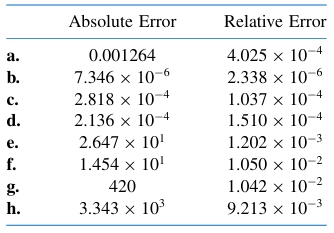
\includegraphics[width=8cm]{Mod1Sec1}
%%\end{center}
%\end{mysolution}
%
%
%%\begin{mysolution}
%%\begin{enumerate}[label=(\alph*)]
%%%\item  Absolute error is
%%%\[\left|\pi-\frac{22}{7}\right|=0.001264\]
%%%Relative error is
%%%\[\frac{\left|\pi-\frac{22}{7}\right|}{\pi}=4.025\times 10^{-4}\]
%%%\item Absolute error is
%%%\[\left|\pi-3.1416\right|=0.7346\times10^{-5}\]
%%%Relative error is
%%%\[\frac{\left|\pi-3.1416\right|}{\pi}=2.338\times 10^{-6}\]
%%%\item Absolute error is
%%%\[\left|e-2.718\right|=0.2818\times10^{-3}\]
%%%Relative error is
%%%\[\frac{\left|e-2.718\right|}{e}=1.037\times 10^{-4}\]
%%%\item Absolute error is
%%%\[\left|\sqrt{2}-1.414\right|=0.2136\times10^{-3}\]
%%%Relative error is
%%%\[\frac{\left|\sqrt{2}-1.414\right|}{\sqrt{2}}=1.510\times 10^{-4}\]
%%%\item Absolute error is
%%%\[\left|e^{10}-22000\right|=0.2647\times10^{2}\]
%%%Relative error is
%%%\[\frac{\left|e^{10}-22000\right|}{e^{10}}=1.202\times 10^{-3}\]
%%\item [(f)] Absolute error is
%%\[\left|10^{\pi}-1400\right|=0.1454\times10^{2}\]
%%Relative error is
%%\[\frac{\left|10^{\pi}-1400\right|}{10^{\pi}}=1.050\times 10^{-2}\]
%%\item [(g)] Absolute error is
%%\[\left|8!-39900\right|=0.42\times10^{3}\]
%%Relative error is
%%\[\frac{\left|8!-39900\right|}{8!}=1.047\times 10^{-2}\]
%%\item [(h)] Absolute error is
%%\[\left|9!-\sqrt{18 \pi}(9 / e)^{9}\right|=0.3343\times10^{4}\]
%%Relative error is
%%\[\frac{\left|9!-\sqrt{18 \pi}(9 / e)^{9}\right|}{9!}=9.213\times 10^{-3}\]
%%\end{enumerate}
%%\end{mysolution}
%
%
%
%
%
%
%
%
%%\activities
%%Read on Finite-digit arithmetic and nested arithmetic in pages \textcolor{red}{\bf page $22-28$} and then attempt the subsequent quiz
%%\begin{activity}[\cg Reading]
%%\begin{enumerate}
%%\item Burden, R. L., Faires, J. D., Burden, A. M. (2015). Numerical Analysis. Tenth Edition, Cengage Learning.\\
%%\end{enumerate}
%%\end{activity}
%%\mylink{https://www.youtube.com/watch?v=cK1WTCA6EpQ}
%
%
%
%
%
%%\begin{figure}[h]
%%\centering
%%\begin{tikzpicture}[line cap=round,line join=round,scale=0.7]
%%%\filldraw[color=gray] plot[domain=-1:2] (\x,{(\x)^2-2*(\x)});
%%%\filldraw[color=gray] plot[domain=-1:2] (\x,{4-(\x)^2});
%%%\filldraw[color=blue!20] plot[domain=1.57:4.7] (\x,{cos(\x r)});
%%%\draw[color=cyan,smooth,ultra thick] plot[domain=0.6:4.2] (\x,{2*cos(\x r)});
%%%\filldraw[color=gray] plot[domain=1.57:4.2] (\x,{-2*cos(\x r)}) -- (4.2,0);
%%\filldraw [color=gray!30!] (-4,3) -- (3,-4) -- ((4,-4) -- (4,3) -- (-4,3);
%%\draw[>=latex,->,color=black] (-4,0) -- (4,0)node[below] { $x$};
%%\draw[>=latex,->,color=black] (0,-4) -- (0,3)node[left] { $y$};
%%\draw[ultra thick,dashed,color=black] (1,-2) -- (1,3);
%%\draw[color=cyan,smooth,ultra thick] plot[domain=-4:3] (\x,{-(\x)-1});
%%%\draw[color=red,smooth,ultra thick] plot[domain=-2.5:2.5] (\x,{4-(\x)^2}) node [black, right] {\scriptsize $y=4-x^2$};
%%
%%%\filldraw [red] (2,0) circle (3pt);
%%
%%%\draw[ultra thick] (4.2,-1.05) -- (4.2,1.05);
%%%%\draw[dashed] (6.283,0) -- (6.283,1);
%%%%\foreach \y in {1,-1}
%%%%\draw[shift={(0,\y)},color=black] (2pt,0pt) -- (-2pt,0pt) node[left] {\footnotesize $\y$};
%%%%\draw[color=black] (0pt,-5pt) node[left] {\footnotesize $0$};
%%%
%%\draw[>=latex,->,color=black] (-1.5,3.2) -- (-2,1);
%%\draw(-1,0) node[below] {\scriptsize $-1$};
%%\draw(0,-1) node[left] {\scriptsize $-1$};
%%\draw(0,0) node[below left] {\scriptsize $0$};
%%\draw(1,2) node[right] {\scriptsize $x=1$};
%%\draw(-1.5,3.2) node [above] {\scriptsize $y=-x-1$};
%%%\draw(2.9,-0.5) node[] { $A_2$};
%%%\draw(1,0.8) node[above] { \scriptsize $y=\cos x$};
%%%\draw(2.9,2.2) node[above] { $y=|f(f)|$};
%%\end{tikzpicture}
%%\caption{\scriptsize Graph of $f(x,y)=\frac{\sqrt{x+y+1}}{x-1}$}
%%\label{firstexamplea}
%%\end{figure}
%
%
%%\begin{figure}%[h]
%%\centering
%%\begin{tikzpicture}[scale=1.5]
%%%\filldraw [color=gray!30!] (-2,-2) -- (-2,2) -- (2,2) -- (2,-2) -- (-2,-2);
%%    \draw[->] (-2,0) -- (2,0) node[right] {$x$};
%%    \draw[->] (0,-2) -- (0,2) node[above] {$y$};
%%    \draw[domain=0:1.5, smooth, variable=\x,blue] plot ({\x},{sqrt(\x)});
%%    \draw[domain=0:1.5, smooth, variable=\x,blue] plot ({\x},{-sqrt(\x)});
%%    \draw[dashed] (0,1.5) -- (1.5,1.5) node[right] {$y^2 = x$};
%%    \draw[dashed] (1.5,0) -- (1.5,1.5);
%%\end{tikzpicture}
%%\caption{\scriptsize Graph of $f(x,y)=x\ln(y^2-x)$}
%%\label{firstexampleb}
%%\end{figure}
%
%
%
%\section{Algorithms and Convergence}
%\begin{youtube}[]
%Watch the following video on  a discussion on algorithms and \\convergence as applied to numerical methods then attempt\\ the subsequent quiz.\\
%\mylink{https://www.youtube.com/watch?v=w7bJIRbgTvA\&t=51s}
%\end{youtube}
%\begin{myexercise}\label{Comprehensionquiz2}
%\begin{enumerate}[label=(\alph*)]
%\item Use three-digit chopping arithmetic to compute the sum $\sum_{i=1}^{10} 1 / i^{2}$ first by $\frac{1}{1}+\frac{1}{4}+\cdots+\frac{1}{100}$ and then by $\frac{1}{100}+\frac{1}{81}+\cdots+\frac{1}{1}$. Which method is more accurate, and why?
%\item Write an algorithm to sum the finite series $\sum^N_{i=1}x_i$ in reverse order.
%\end{enumerate}
%
%
%\begin{mysolution}
%\begin{enumerate}[label=(\alph*)]
%\item The forward order sum is
%\begin{center}
%\begin{tabular}{|l|l|l|}\hline
%$1/i^2$&Chopped Value&Running Total\\\hline
%$1$&$1.00$&$1.00$\\
%$0.25$&$0.250$&$1.00+0.250=1.25$\\
%$0.\bar{1}$&$0.111$&$1.25+0.111=1.36$\\
%$0.0625$&$0.062$&$1.36+0.062=1.42$\\
%$0.04$&$0.040$&$1.42+0.04=1.46$\\
%$0.02\bar{7}$&$0.027$&$1.46+0.027=1.48$\\
%$0.0204\ldots$&$0.020$&$1.48+0.020=1.50$\\
%$0.015625$&$0.015$&$1.50+0.015=1.51$\\
%$0.012345\ldots$&$0.012$&$1.51+0.012=1.52$\\
%$0.01$&$0.010$&$1.52+0.010=1.53$\\\hline
%\end{tabular}
%\end{center}
%%The backward order sum is
%%\begin{center}
%%\begin{tabular}{|l|l|l|}\hline
%%$1/i^2$&Chopped Value&Running Total\\\hline
%%$0.01$&$0.010$&$0.010$\\
%%$0.012345\ldots$&$0.012$&$0.010+0.012=0.022$\\
%%$0.015625$&$0.015$&$0.022+0.015=0.037$\\
%%$0.0204\ldots$&$0.020$&$0.037+0.020=0.057$\\
%%$0.02\bar{7}$&$0.027$&$0.057+0.027=0.084$\\
%%$0.04$&$0.040$&$0.084+0.04=0.124$\\
%%$0.0625$&$0.062$&$0.124+0.062=0.186$\\
%%$0.\bar{1}$&$0.111$&$0.186+0.111=0.297$\\
%%$0.25$&$0.250$&$0.297+0.250=0.547$\\
%%$1$&$1.00$&$0.5471.00=1.54$\\\hline
%%\end{tabular}
%%\end{center}
%%
%%
%%The exact value is
%%\[\sum_{i=1}^{10}(1/i^2)=1.54976773117\]
%
%\end{enumerate}
%\end{mysolution}
%
%%\newpage
%
%\begin{mysolution}
%\begin{enumerate}[label=(\alph*)]
%\item[]
%The backward order sum is
%\begin{center}
%\begin{tabular}{|l|l|l|}\hline
%$1/i^2$&Chopped Value&Running Total\\\hline
%$0.01$&$0.010$&$0.010$\\
%$0.012345\ldots$&$0.012$&$0.010+0.012=0.022$\\
%$0.015625$&$0.015$&$0.022+0.015=0.037$\\
%$0.0204\ldots$&$0.020$&$0.037+0.020=0.057$\\
%$0.02\bar{7}$&$0.027$&$0.057+0.027=0.084$\\
%$0.04$&$0.040$&$0.084+0.04=0.124$\\
%$0.0625$&$0.062$&$0.124+0.062=0.186$\\
%$0.\bar{1}$&$0.111$&$0.186+0.111=0.297$\\
%$0.25$&$0.250$&$0.297+0.250=0.547$\\
%$1$&$1.00$&$0.5471.00=1.54$\\\hline
%\end{tabular}
%\end{center}
%Thus
%\begin{center}
%\begin{tabular}{|l|l|l|}\hline
%Method&Sum&Absolute Error\\\hline
%Forward sum&$1.53$&$approx0.0198$\\
%Backward sum&$1.54$&$approx0.0098$\\\hline
%\end{tabular}
%\end{center}
%Hence the backward sum is more accurate. This is due to loss of significance in floating-point arithmetic.
%
%\begin{itemize}
%\item In forward order, large numbers (e.g., $1.00$) are added first.
%\item Later, small values (like $0.01$) may get lost due to limited precision; adding them to a large total may have no effect after chopping.
%\item In reverse order, we add small numbers first, so their contributions are preserved early in the summation.
%\item Later, adding large values doesn't suffer as much from chopping.
%\end{itemize}
%This is a classic example of numerical stability: summing from smallest to largest reduces round-off error.
%\item [(b)] Here is the algorithm
%
%\begin{boxB}
%Algorithm ReverseSum(x, N):\\
%Input: Array $x[1\ldots N]$ containing the series terms\\
%Output: Sum of the series $\sum_{i=1}^N x_i$, computed in reverse order\\
%\\
%Step 1 Set SUM=0\\
%Step 2 For $i=N, \ldots, 1$\\
%\hspace*{1cm} Set SUM=SUM+x\_i\\
%Step 3 Output (SUM)\\
%\hspace*{1cm} STOP
%\end{boxB}
%\end{enumerate}
%\end{mysolution}
%\end{myexercise}
%
%\section{Solution of Equations of One Variable}
%\videolesson
%\begin{selfvideo}[2]
%%LESSON 3: 
%This video covers bisection method for solving equation of one variable. Follow the discussion and attempt the quiz that follows.
%\end{selfvideo}
%%\begin{boxB}Question: Which are the determining factors for the temperature of a given location on the surface of the earth at a given time?\end{boxB}
%In this section we consider one of the most basic problems of numerical approximation, the {\bf root-finding problem}. This process involves finding a {\bf root}, or solution, of an equation of the form $f(x)=0$, for a given function $f$. A root of this equation is also called a {\bf zero} of the function $f$.
%
%\subsection*{Bisection Technique}
%Suppose $f$ is a continuous function defined on the interval $[a,b]$, with $f(a)$ and $f(b)$ of opposite sign. The Intermediate Value Theorem implies that a number $p$ exists in $(a,b)$ with $f(p) = 0$. Although the procedure will work when there is more than one root in the interval $(a, b)$, we assume for simplicity that the root in this interval is unique. The method calls for a repeated halving (or bisecting) of subintervals of $[a,b]$ and, at each step, locating the half containing $p$.
%
% To begin, set $a_1 = a$ and $b_1 = b$, and let $p_1$ be the midpoint of $[a,b]$; that is,
%\[p_1=a_1+\frac{b_1-a_1}{2}=\frac{a_1+b_1}{2}.\]
%\begin{itemize}
%\item If $f(p_1)=0$, then $p=p_1$, and we are done.
%\item If $f(p_1)\neq0$, then $f(p_1)$ has the same sign as either $f(a_1)$ or $f(b_1)$.
%\item If $f\left(p_{1}\right)$ and $f\left(a_{1}\right)$ have the same sign, $p\in(p_1,b_1)$. Set $a_{2}=p_{1}$ and $b_{2}=b_{1}$.
%\item If $f\left(p_{1}\right)$ and $f\left(a_{1}\right)$ have opposite signs, then $p\in(a_1,p_1)$. Set $a_{2}=a_{1}$ and $b_{2}=p_{1}$.
%\end{itemize}
%
%Then reapply the process to the interval $\left[a_{2}, b_{2}\right]$. (See Figure below)
%
%%%\begin{myalgorithm}
%%%\underline{To find a solution to $f(x) = 0$ given the continuous function $f$ on the interval $[a,b]$, where}\\
%%%\underline{ $f(a)$ and $f(b)$ have opposite signs:}\\
%%%%\begin{tabular}{ll}
%%%INPUT {\it endpoints $a, b$; tolerance TOL; maximum number of iterations $N_0$.}\\
%%%OUTPUT {\it approximate solution p or message of failure.}\\
%%%%\end{tabular}
%%%Step 1\hspace{1cm} Set $i=1$;\\
%%%\hspace{4cm} $FA=f(a)$\\
%%%Step 2\hspace{2cm} While $i\leq N_0$ do Steps $3-6$.\\
%%%~~~~~~Step 3\hspace{1cm} Set $p=a+(b-a)/2$; \hspace{1cm} ({\it Compute $p_i$})
%%%\hspace{5cm}
%%%\end{myalgorithm}
%%
%%\begin{tcolorbox}
%%\underline{\bf ALGORITHM $1$ To find a solution to $f(x) = 0$ given the continuous function $f$ on the}\\
%%\underline{\bf interval $[a,b]$, where $f(a)$ and $f(b)$ have opposite signs:}\\
%%INPUT {\it endpoints $a, b$; tolerance $TOL$; maximum number of iterations $N_0$.}\\
%%OUTPUT {\it approximate solution p or message of failure.}\\
%%Step 1 Set $i=1$;\\
%%\hspace*{2cm} $FA=f(a)$.\\
%%Step 2 While $i\leq N_0$ do Steps $3 - 6$.\\
%%\hspace*{1cm} Step 3 Set $p=a+(b-a)/2$; ({\it Compute$p_i$}.)\\
%%\hspace*{3cm}$FP=f(p)$.\\
%%\hspace*{1cm}  Step 4 If $FP=0$ or $(b-a)/2<TOL$ then \\
%%\hspace*{3cm} OUTPUT $(p)$; ({\it Procedure completed successfully}.)\\
%%\hspace*{3cm} STOP.\\
%%\hspace*{1cm} Step 5 Set $i=i+1$.\\
%%\hspace*{1cm} Step 6 If $FA\cdot FP>0$ then set $a=p$; ({\it Compute $a_i$, $b_i$.})\\
%%\hspace*{5cm} $FA=FP$\\
%%\hspace*{4cm} else set $b=p$. ({\it $FA$ is unchanged}.)\\
%%Step 7 OUTPUT (`Method failed after $N_0$ iterations, $N_0=', N_0$);\\
%%\hspace*{1cm} ({\it The procedure was unsuccessful}.)\\
%%\hspace*{1cm} STOP
%%\end{tcolorbox}
%
%\begin{figure}[h]
%\centering
%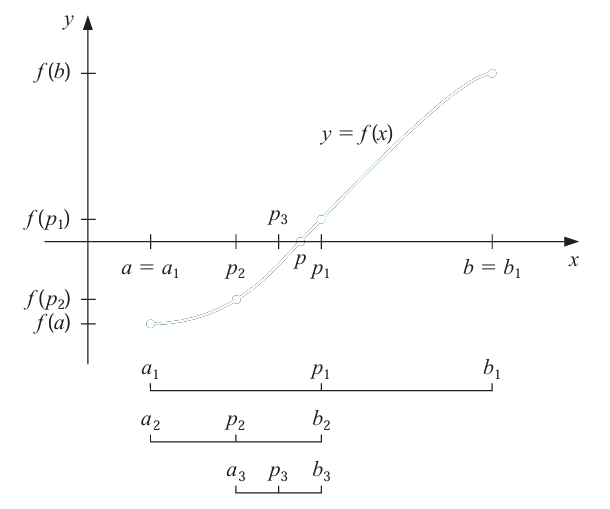
\includegraphics[ width=10cm]{Bisectionmethodpicture1.jpeg}
%\caption{\scriptsize }
%\label{}
%\end{figure}
%
%
%
%
%
%
%
%%[Bisection Method] An interval $\left[a_{n+1}, b_{n+1}\right]$ containing an approximation to a root of $f(x)=0$ is constructed from an interval $\left[a_{n}, b_{n}\right]$ containing the root by first letting
%%
%%$$
%%p_{n}=a_{n}+\frac{b_{n}-a_{n}}{2}
%%$$
%%
%%Then set
%%
%%$$
%%a_{n+1}=a_{n} \quad \text { and } \quad b_{n+1}=p_{n} \quad \text { if } \quad f\left(a_{n}\right) f\left(p_{n}\right)<0
%%$$
%%
%%and
%%
%%$$
%%a_{n+1}=p_{n} \quad \text { and } \quad b_{n+1}=b_{n} \quad \text { otherwise. }
%%$$
%%
%%There are three stopping criteria commonly incorporated in the Bisection method. First, the method stops if one of the midpoints happens to coincide with the root. It also stops when the length of the search interval is less than some prescribed tolerance we call $T O L$. The procedure also stops if the number of iterations exceeds a preset bound $N_{0}$.
%%
%%To start the Bisection method, an interval $[a, b]$ must be found with $f(a) \cdot f(b)<$ 0 . At each step, the length of the interval known to contain a zero of $f$ is reduced by a factor of 2 . Since the midpoint $p_{1}$ must be within $(b-a) / 2$ of the root $p$, and each succeeding iteration divides the interval under consideration by 2 , we have
%%
%%$$
%%\left|p_{n}-p\right| \leq \frac{b-a}{2^{n}}
%%$$
%%
%%As a consequence, it is easy to determine a bound for the number of iterations needed to ensure a given tolerance. If the root needs to be determined within the tolerance TOL, we need to determine the number of iterations, $n$, so that
%%
%%$$
%%\frac{b-a}{2^{n}}<T O L
%%$$
%%
%%Solving for $n$ in this inequality gives
%%
%%$$
%%\frac{b-a}{T O L}<2^{n}, \quad \text { which implies that } \quad \log _{2}\left(\frac{b-a}{\mathrm{TOL}}\right)<n .
%%$$
%%
%%Since the number of required iterations to guarantee a given accuracy depends on the length of the initial interval $[a, b]$, we want to choose this interval as small as possible. For example, if $f(x)=2 x^{3}-x^{2}+x-1$, we have both
%%
%%$$
%%f(-4) \cdot f(4)<0 \quad \text { and } \quad f(0) \cdot f(1)<0
%%$$
%%
%%so the Bisection method could be used on either $[-4,4]$ or $[0,1]$. Starting the Bisection method on $[0,1]$ instead of $[-4,4]$ reduces by 3 the number of iterations required to achieve a specified accuracy.
%%\end{itemize}
%\begin{example}
%Show that $f(x) = x^3 +4x^2 -10 = 0$ has a root in $[1,2]$, and use the Bisection method to determine an approximation to the root that is accurate to at least within $10^{-4}$.
%\end{example}
%
%\begin{mysolution}
%Because $f(1) =-5$ and $f(2) = 14$ the Intermediate Value Theorem ensures that this continuous function has a root in $[1,2]$. 
%
%For the first iteration of the Bisection method we use the fact that at the midpoint of $[1, 2]$ we have $f(1.5) = 2.375 > 0$. This indicates that we should select the interval $[1,1.5]$ for our second iteration. Then we find that $f(1.25) =-1.796875$ so our new interval becomes $[1.25,1.5]$, whose midpoint is $1.375$. Continuing in this manner gives the values in Table \ref{}. After $13$ iterations, $p_{13} = 1.365112305$ approximates the root $p$ with an error
%\[|p-p_{13}|<|b_{14}-a_{14}|=|1.365234375-1.365112305|=0.000122070.\]
%Since $|a_{14}|<|p|$, we have
%\[\frac{|p-p_{13}|}{|p|}<\frac{|b_{14}-a_{14}|}{|a_{14}|}\leq9.0\times10^{-5},\]
%so the approximation is correct to atleast within $10^{-4}$. The correct value of $p$ to nine decimal  places is $p=1.365230013$. Note that $p_9$ is closer to $p$ than is the final approximation $p_{13}$.
%
%\begin{center}
%\centering
%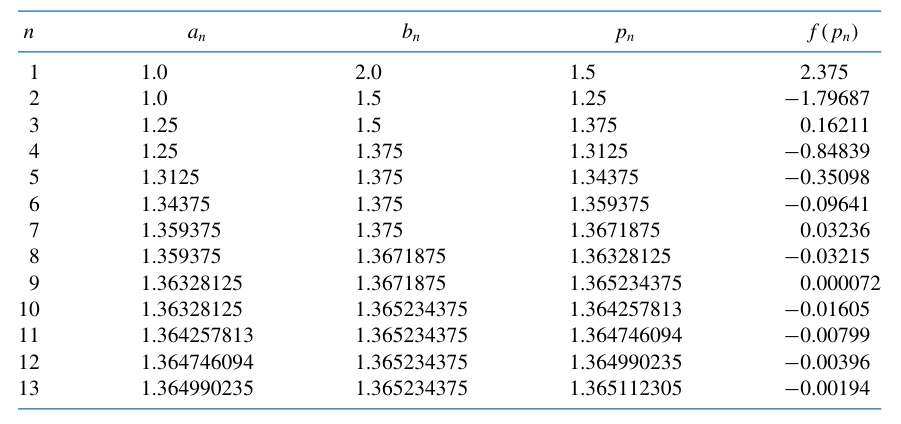
\includegraphics[ width=13cm]{Bisectionmethodexampletable.jpeg}
%%\caption{\scriptsize }
%%\label{}
%\end{center}
%\end{mysolution}
%
%\begin{theorem}
%Suppose that $f\in C[a, b]$ and $f(a)\cdot f(b)<0$. The Bisection method generates a sequence $\left\{p_n\right\}_{n=1}^{\infty}$ approximating a zero $p$ of $f$ with
%\[|p_n-p|\leq\frac{b-a}{2^n},\quad\mbox{when}\quad n\geq1.\]
%\end{theorem}
%
%\begin{example}
%Determine the number of iterations necessary to solve $f(x) = x^3 + 4x^2 - 10 = 0$ with accuracy $10^{-3}$  using $a_1 = 1$ and $b_1 = 2$.
%\end{example}
%
%\begin{mysolution}
%We we will use logarithms to find an integer $N$ that satisfies
%\[|p_N-p|\leq2^{-N}(b-a)=2^{-N}<10^{-3}.\]
%Logarithms to any base would suffice, but we will use base$-10$ logarithms because the tolerance is given as a power of $10$. Since $2^{-N}<10^{-3}$ implies that $\log_{10}2^{-N}<\log_{10}10^{-3} =-3$, we have
%\[-N\log_{10}2<-3\quad\mbox{and}\quad N>\frac{3}{\log_{10}2}\approx9.96.\]
%Hence, ten iterations will ensure an approximation accurate to within $10^{-3}$.
%
%Table \ref{} shows that the value of $p_9 = 1.365234375$ is accurate to within $10^{-4}$. Again, it is important to keep in mind that the error analysis gives only a bound for the number of iterations. In many cases this bound is much larger than the actual number required.
%\end{mysolution}
%
%\begin{myexercise}\label{Comprehensionquiz2}
%\begin{enumerate}[label=\arabic*.]
%\item Use the Bisection method to find $p_{3}$ for $f(x)=\sqrt{x}-\cos x$ on $[0,1]$. 
%\item Use the Bisection method to find solutions accurate to within $10^{-2}$ for $x^{3}-$ $7 x^{2}+14 x-6=0$ on each interval.
%\begin{multicols}{3}
%\begin{enumerate}[label=(\alph*)]
%\item $[0,1]$
%\item $[1,3.2]$
%\item $[3.2,4]$
%\end{enumerate}
%\end{multicols}
%\end{enumerate}
%
%\begin{mysolution}
%\begin{enumerate}[label=\arabic*.]
%\item Here $f(0)=-1<0$ and $f(1)=0.45969769413>0$. The sequence of approximate solutions are tabulated below
%
%\begin{center}
%\begin{tabular}{lllll}\hline
%$n$&$a_n$&$b_n$&$p_n$&$f(p_n)$\\
%$1$&$0$&$1$&$0.5$&$-0.1704757807$\\
%$2$&$0.5$&$1$&$0.75$&$0.13433653491$\\
%$3$&$0.5$&$0.75$&$0.625$&$-0.02039370446$\\\hline
%\end{tabular}
%\end{center}
%$p_3=0.625$
%
%\item 
%\begin{enumerate}[label=(\alph*)]
%\item Here $a=0$ and $b=1$ so that $2^{-n}<10^{-2}$. Applying natural logarithm to both sides of the inequality yields $log_{10}2^{-n}<log_{10}10^{-2}$. Solving for $n$ yields 
%\[n>\frac{2}{log_{10}2}=6.643\ldots\]
%
%Thus $n=7$. Here $f(0)=-6<0$ and $f(1)=2>0$. The sequence of approximate solutions are tabulated below
%\end{enumerate}
%\end{enumerate}
%\end{mysolution}
%%
%\begin{mysolution}
%\begin{enumerate}
%\item[]
%
%\begin{center}
%\begin{tabular}{lllll}\hline
%$n$&$a_n$&$b_n$&$p_n$&$f(p_n)$\\
%$1$&$0$&$1$&$0.5$&$-0.625$\\
%$2$&$0.5$&$1$&$0.75$&$0.984375$\\
%$3$&$0.5$&$0.75$&$0.625$&$0.259765625$\\
%$4$&$0.5$&$0.625$&$0.5625$&$-0.16186523438$\\
%$5$&$0.5625$&$0.625$&$0.59375$&$0.29712163086$\\
%$6$&$0.5625$&$0.59375$&$0.578125$&$-0.05262374878$\\\hline
%\end{tabular}
%\end{center}
%
%\vspace{3mm}
%$p_7=\frac{0.578125+0.59375}{2}=0.5859$ 
%
%\begin{enumerate}
%\item[(b)] Here $a=1$ and $b=3.2$ so that $2^{-n}\cdot2.2<10^{-2}$. Applying natural logarithm to both sides of the inequality yields $log_{10}2^{-n}<log_{10}10^{-2}-log_{10}2.2$. Solving for $n$ yields 
%\[n>\frac{2+log_{10}2.2}{log_{10}2}=7.781\]
%Thus $n=8$. Here $f(1)=2>0$ and $f(3.2)=-0.112<0$. The sequence of approximate solutions are tabulated below
%\begin{center}
%\begin{tabular}{lllll}\hline
%$n$&$a_n$&$b_n$&$p_n$&$f(p_n)$\\
%$1$&$1$&$3.2$&$2.1$&$1.791$\\
%$2$&$2.1$&$3.2$&$2.65$&$0.552125$\\
%$3$&$2.65$&$3.2$&$2.925$&$0.085828125$\\
%$4$&$2.925$&$3.2$&$3.0625$&$-0.5444335938$\\
%$5$&$2.925$&$3.0625$&$2.99375$&$0.00632788086$\\
%$6$&$2.99375$&$3.0625$&$3.028125$&$-0.02652072144$\\
%$7$&$2.99375$&$3.028125$&$3.0109375$&$-0.01069693375$\\\hline
%\end{tabular}
%\end{center}
%%\end{enumerate}
%%\end{enumerate}
%%\end{mysolution}
%%
%%\begin{mysolution}
%%\begin{enumerate}
%%\item[]
%%\begin{enumerate}
%%\item[]
%$p_8=\frac{2.99375+3.028125}{2}=3.002$
%
%\vspace{5mm}
%
%
%\item [(c)] Here $a=3.2$ and $b=4$ so that $2^{-n}\cdot0.8<10^{-2}$. Applying natural logarithm to both sides of the inequality yields $log_{10}2^{-n}<log_{10}10^{-2}-log_{10}0.8$. Solving for $n$ yields 
%\[n>\frac{2+log_{10}0.8}{log_{10}2}=6.32192\ldots\]
%Thus $n=7$. Here $f(3.2)=-0.112<0$ and $f(4)=2>0$. The sequence of approximate solutions are tabulated below
%\begin{center}
%\begin{tabular}{lllll}\hline
%$n$&$a_n$&$b_n$&$p_n$&$f(p_n)$\\
%$1$&$3.2$&$4$&$3.6$&$0.336$\\
%$2$&$3.2$&$3.6$&$3.4$&$-0.016$\\
%$3$&$3.4$&$3.6$&$3.5$&$0.125$\\
%$4$&$3.4$&$3.5$&$3.45$&$0.046125$\\
%$5$&$3.4$&$3.45$&$3.425$&$0.013015625$\\
%$6$&$3.4$&$3.425$&$3.4125$&$-0.00199804688$\\\hline
%\end{tabular}
%\end{center}
%
%\vspace{3mm}
%$p_7=\frac{3.4125+3.425}{2}=3.419$
%\end{enumerate}
%\end{enumerate}
%\end{mysolution}
%\end{myexercise}
% 
%
%\section{Fixed Point Iteration and Newton's Method}
%\activities
%Read on Newton's Method and its extensions in pages in the link below and then attempt the subsequent quiz
%\begin{activity}[\cg Reading]
%%\begin{enumerate}
%%\textcolor{red}{\bf page $934-946$}
%%\item Ryan T. White and Archana Tikayat Ray, (2021), {\it Practical Discrete Mathematics: Discover math principles that fuel algorithms for computer science and machine learning with Python}, Packt Publishing,  ISBN-13 ‏ : ‎ 978-1838983147 \\
%%\textcolor{red}{\bf pages $23-30$}
%%\item S. Lipschutz and M. Lipson, (2021), {\it Schaum’s Outline of Discrete Mathematics}, Fourth Edition (Schaum’s Outlines) 4th Edition, McGraw Hill, ISBN-13: 978-1264258802\\
%%\textcolor{red}{\bf pages $70-76$}
%%\end{enumerate}
%\end{activity}
%\mylink{https://pythonnumericalmethods.studentorg.berkeley.edu/notebooks/chapter19.04-Newton-Raphson-Method.html}\\
%\begin{youtube}[]
%Watch the following video on  a discussion on Fixed-Point Iteration then attempt the subsequent quiz.\\
%\mylink{https://www.youtube.com/watch?v=I-B9MGK3gwU}
%\end{youtube}
%
%\begin{myexercise}\label{Comprehensionquiz2}
%\begin{enumerate}[label=\arabic*.]
%\item Use algebraic manipulation to show that each of the following functions has a fixed point at $p$ precisely
% when $f(p) = 0$, where $f(x) = x^4 +2x^2-x-3$.
%\begin{multicols}{2}
%\begin{enumerate}[label=(\alph*)]
%\item $g_1(x)=(3+x-2x^2)^{1/4}$\\[5mm]
%\item $g_2(x)=\left(\frac{x+3-x^4}{2}\right)^{1/2}$
%\item $g_3(x)=\left(\frac{x+3}{x^2+2}\right)^{1/2}$\\[4mm]
%\item $g_4(x)=\frac{3x^4+2x^2+3}{4x^4+4x-1}$
%\end{enumerate}
%\end{multicols}
%\item Let $f(x)=x^2−6$ and $p_0=1$. Use Newton’s method to find $p_2$.
%\begin{mysolution}
%\begin{enumerate}[label=(\alph*)]
%\item For the value of $x$ under consideration we have
%%\begin{multicols}{2}
%\begin{enumerate}[label=\arabic*.]
%\item $x =(3+x-2x^2)^{1/4}\quad\Leftrightarrow\quad x^4 = 3+x-2x^2\quad\Leftrightarrow\quad f(x) = 0$\\
%\item $x =\left(\frac{x+3-x^4}{2}\right)^{1/2}\quad\Leftrightarrow\quad 2x^2 = x+3-x^4\quad\Leftrightarrow\quad f(x) = 0$\\
%\item $x =\left(\frac{x+3}{x^2+2}\right)^{1/2}\quad\Leftrightarrow\quad x^2(x^2+2)= x+3\quad\Leftrightarrow\quad f(x) = 0$\\
%\item $x =\frac{3x^4+2x^2+3}{4x^3+4x-1}\quad\Leftrightarrow\quad 4x^4+4x^2-x= 3x^4+2x^2+3\quad\Leftrightarrow\quad f(x) = 0$
%\end{enumerate}
%%\end{multicols}
%\item $p_2=2.60714$
%\end{enumerate}
%\end{mysolution}
%\end{enumerate}
%\end{myexercise}
%
%
%
%
%
%
%%%%%%%%%%%%%%%%%%%%%%%%%%%%%%%%%%%%%%%%%%%%%%%%%%%%%%%%%%%%%%%%%%%%%%%%%%%%%%%%%%%%%%%%%%%%%%%%%%%%%%%%%%%%%%%%%%%%%%%%%%%%%%%%%%%%%%%%%%%%%%%
%
%
%
%%\bibliographystyle{unsrt} \bibliography{bibliography}
%
%%\activities
%%The following reading is necessary for your constructive engagement in the group discussion.
%%\begin{activity}[\cg Reading]
%%\begin{enumerate}
%%\item Burden, R. L., Faires, J. D., Burden, A. M. (2015). Numerical Analysis. Tenth Edition, Cengage Learning.\\
%%%\textcolor{red}{\bf page $934-946$}
%%%\item Ryan T. White and Archana Tikayat Ray, (2021), {\it Practical Discrete Mathematics: Discover math principles that fuel algorithms for computer science and machine learning with Python}, Packt Publishing,  ISBN-13 ‏ : ‎ 978-1838983147 \\
%%%\textcolor{red}{\bf pages $23-30$}
%%%\item S. Lipschutz and M. Lipson, (2021), {\it Schaum’s Outline of Discrete Mathematics}, Fourth Edition (Schaum’s Outlines) 4th Edition, McGraw Hill, ISBN-13: 978-1264258802\\
%%%\textcolor{red}{\bf pages $70-76$}
%%\end{enumerate}
%%\end{activity}
%
%%\discussion
%%Discuss how you would solve questions 71-75 in Exercise 14.1 of indicated reference.
%
%%\begin{enumerate}
%%\item Render the implication in English language.
%%\item\label{Discusion1} Determine the converse, contrapositive and inverse of the implication $u\rightarrow v$  in symbolic notation in terms of the component propositions
%%\item Express each of the implications obtained in \ref{Discusion1} English language
%%\end{enumerate}
%
%
%%Let $p$, $q$, $r$, and $s$ be the following propositions
%%\[\begin{split}
%%p:&~ \mbox{Grizzly bears have been seen in the area.}\\
%%q:&~  \mbox{Hiking is safe on the trail.}\\
%%r:&~  \mbox{Berries are ripe along the trail.}\\
%%s:&~  \mbox{You drive over 65 miles per hour.}
%%\end{split}\]
%%
%%Consider the following implication $u\rightarrow v$ where
%%\[u:\neg(p\lor q)\quad\mbox{ and }\quad v:r\lor\neg s.\]
%
%%\begin{enumerate}
%%\item Render the implication in English language.
%%\item\label{Discusion1} Determine the converse, contrapositive and inverse of the implication $u\rightarrow v$  in symbolic notation in terms of the component propositions
%%\item Express each of the implications obtained in \ref{Discusion1} English language
%%\end{enumerate}
%%Thank you and keep safe!
%
%\begin{posttest}[\textcolor{red}{End of Module One Quiz}]
%\item Suppose $p^*$ must approximate $p$ with relative error at most $10^{-3}$. Find the largest interval in which $p^*$ must lie for each value of $p$.
%\begin{multicols}{4}
%\begin{enumerate}[label=(\alph*)]
%\item $150$
%\item $900$
%\item $1500$
%\item $90$
%\end{enumerate}
%\end{multicols}
%\begin{mysolution}
%\begin{enumerate}[label=(\alph*)]
%\item[]
%\[\frac{|p^*-p|}{|p|}\leq10^{-3}\quad\Longleftrightarrow\quad p\left(1-10^{-3}\right)\leq p^*\leq p\left(1+10^{-3}\right)\]
%\item Here $p=150$ so that $p\left(1-10^{-3}\right)=150\left(1-10^{-3}\right)=149.85$ and $p\left(1+10^{-3}\right)=150\left(1+10^{-3}\right)=150.15$. Hence the required interval is $(149.85,150.15)$
%\item Here $p=900$ so that $p\left(1-10^{-3}\right)=900\left(1-10^{-3}\right)=899.1$ and $p\left(1+10^{-3}\right)=900\left(1+10^{-3}\right)=900.9$. Hence the required interval is $(899.1,900.9)$
%\item Here $p=1500$ so that $p\left(1-10^{-3}\right)=1500\left(1-10^{-3}\right)=1498.5$ and $p\left(1+10^{-3}\right)=1500\left(1+10^{-3}\right)=1501.5$. Hence the required interval is $(1498.5,1501.5)$
%\item Here $p=90$ so that $p\left(1-10^{-3}\right)=90\left(1-10^{-3}\right)=89.91$ and $p\left(1+10^{-3}\right)=90\left(1+10^{-3}\right)=90.09$. Hence the required interval is $(89.91,90.09)$
%\end{enumerate}
%
%\end{mysolution}
%\item The Maclaurin series for the arctangent function converges for $-1<x \leq 1$ and is given by
%
%$$
%\arctan x=\lim _{n \rightarrow \infty} P_{n}(x)=\lim _{n \rightarrow \infty} \sum_{i=1}^{n}(-1)^{i+1} \frac{x^{2 i-1}}{(2 i-1)}
%$$
%
%\begin{enumerate}[label=(\alph*)]
%\item Use the fact that $\tan \pi / 4=1$ to determine the number of terms of the series that need to be summed to ensure that $\left|4 P_{n}(1)-\pi\right|<10^{-3}$.
%\item The C programming language requires the value of $\pi$ to be within $10^{-10}$. How many terms of the series would we need to sum to obtain this degree of accuracy?
%\end{enumerate}
%\begin{mysolution}
%From the equation
%\[\arctan x=\lim _{n \rightarrow \infty} P_{n}(x)=\lim _{n \rightarrow \infty} \sum_{i=1}^{n}(-1)^{i+1} \frac{x^{2 i-1}}{(2 i-1)}\]
%it follows that 
%\[\frac{\pi}{4}=\arctan 1=\sum_{i=1}^{\infty}\frac{(-1)^{i+1}}{(2 i-1)}\]
%Therefore
%\[\frac{\pi}{4}\approx\sum_{i=1}^{n}\frac{(-1)^{i+1}}{(2 i-1)}\]
%This is an alternating series with terms which are decreasing in magnitude. Thus by the Alternating Series Remainder Theorem, the error $|4P_n(1)-\pi|$ is less than or equal to the absolute value of the first omitted term which is
%\[\left|\frac{(-1)^{(n+1)-1}\cdot 4}{2(n+1)-1}\right|=\frac{4}{2n+1}\]
%\begin{enumerate}[label=(\alph*)]
%\item Here we look for $n$ such that
%\[\frac{4}{2n+1}<10^{-3}\quad\Longleftrightarrow\quad n>\frac{4-10^{-3}}{2\times10^{-3}}=1999.5\]
%Thus the least such integer $n$ is $2000$ which is the required number of terms.
%\item Here we look for $n$ such that
%\[\frac{4}{2n+1}<10^{-10}\quad\Longleftrightarrow\quad n>\frac{4-10^{-10}}{2\times10^{-10}}=19,999,999,999.5\]
%Thus the least such integer $n$ is $20,000,000,000$ which is the required number of terms.
%\end{enumerate}
%\end{mysolution}
%\item Use the Bisection method to find solutions accurate to within $10^{-3}$ for the following problems.
%\begin{enumerate}[label=(\alph*)]
%\item $x-2^{-x}=0$ for $0\leq x\leq1$
%\item $e^x-x^2+3x-2=0$ for $0\leq x\leq1$
%%\item $2x\cos(2x)-(x+1)^2=0$ for $-3\leq x\leq-2$ and $-1\leq x\leq0$.
%%\item $x\cos x-2x^2+3x-1=0$ for $0.2\leq x\leq0.3$ and $1.2\leq x\leq1.3$
%\end{enumerate}
%\begin{mysolution}
%\begin{enumerate}[label=(\alph*)]
%\item Here $a=0$ and $b=1$. So in the inequality $2^{-n}(b-a)<10^{-3}$ becomes $2^{-n}(1-0)<10^{-3}$. Solving for $n$ obtain $n>\frac{3}{log_{10}2}=9.96578428466\ldots$ so that $n=10$.
%
%Now $f(0)=-1<0$ and $f(1)=0.5>0$. The sequence of approximate solutions are tabulated below
%\begin{center}
%\begin{tabular}{lllll}\hline
%$n$&$a_n$&$b_n$&$p_n$&$f(p_n)$\\
%$1$&$0$&$1$&$0.5$&$-0.20710678119$\\
%$2$&$0.5$&$1$&$0.75$&$0.1553964425$\\
%$3$&$0.5$&$0.75$&$0.625$&$-0.02341977733$\\
%$4$&$0.625$&$0.75$&$0.6875$&$0.06657109396$\\
%$5$&$0.625$&$0.6875$&$0.65625$&$0.0217245214$\\
%$6$&$0.625$&$0.65625$&$0.640625$&$-0.00081000804$\\
%$7$&$0.640625$&$0.65625$&$0.6484375$&$0.0074666108$\\
%$8$&$0.640625$&$0.6484375$&$0.64453125$&$0.00483064625$\\
%$9$&$0.640625$&$0.64453125$&$0.642578125$&$0.00201090611$\\\hline
%\end{tabular}
%\end{center}
%
%\vspace{3mm}
%$p_{10}=\frac{0.640625+0.64453125}{2}=0.642578125$
%\item Here $a=0$ and $b-1$. So in the inequality $2^{-n}(b-a)<10^{-3}$ becomes $2^{-n}(1-0)<10^{-3}$. Solving for $n$ obtain $n>\frac{3}{log_{10}2}=9.96578428466\ldots$ so that $n=10$.
%
%Now $f(0)=-1<0$ and $f(1)=2.71828\ldots>0$. The sequence of approximate solutions are tabulated below
%\begin{center}
%\begin{tabular}{lllll}\hline
%$n$&$a_n$&$b_n$&$p_n$&$f(p_n)$\\
%$1$&$0$&$1$&$0.5$&$0.8987212707$\\
%$2$&$0$&$0.5$&$0.25$&$-0.02847458331$\\
%$3$&$0.25$&$0.5$&$0.375$&$0.43936641462$\\
%$4$&$0.25$&$0.375$&$0.3125$&$0.20668169117$\\
%$5$&$0.25$&$0.3125$&$0.28125$&$0.08943319623$\\
%$6$&$0.25$&$0.28125$&$0.265625$&$0.03056423414$\\
%$7$&$0.25$&$0.265625$&$0.2578125$&$0.00106636769$\\
%$8$&$0.25$&$0.2578125$&$0.25390625$&$-0.01369868371$\\
%$9$&$0.25390625$&$0.2578125$&$0.255859375$&$-0.00631480679$\\
%\hline
%\end{tabular}
%\end{center}
%
%
%\vspace{3mm}
%$p_{10}=\frac{0.255859375+0.2578125}{2}=0.2568359375$
%%\item For the interval $[-3,-2]$, we have $p_{17} =-2.191307$, and for the interval $[-1,0]$, we have $p_{17}=-0.798164$.
%%\item For the interval $[0.2,0.3]$, we have $p_{14} =0.297528$, and for the interval $[1.2,1.3]$, we have $p_{14}=1.256622$.
%\end{enumerate}
%\end{mysolution}
%\item Let $f(x) = (x+2)(x+1)x(x-1)^3(x-2)$. To which zero of $f$ does the Bisection method converge when applied on the following intervals?
%\begin{multicols}{4}
% \begin{enumerate}[label=(\alph*)]
%\item $[-3,2.5]$
%\item $[-2.5,3]$
% \item $[-1.75,1.5]$
%\item $[-1.5,1.75]$
%\end{enumerate}
%\end{multicols}
%\begin{mysolution}
% \begin{enumerate}[label=(\alph*)]
%\item Here $a=-3$ and $b=2.5$ with $f(-3)<0$ and $f(2.5)>0$. We determine the zero of convergence in the table below where $m_n=(a_n+b_n)/2$
%
%\begin{center}
%\begin{tabular}{lllclc}\hline
%$n$&$a_n$&$b_n$&Zeros here&$m_n$&Sign of $f(m_n)$\\\hline
%$1$&$-3$&$2.5$&$-2, -1, 0, 1, 2$&$-0.25$&$-$\\
%$2$&$-0.25$&$2.5$&$0, 1, 2$&$1.125$&$-$\\\hline
%\end{tabular}
%\end{center} 
%
%The subsequent interval is $[1.125,2.5]$ and the only zero there is $2$.
%\item Here $a=-2.5$ and $b=3$ with $f(-2.5)<0$ and $f(3)>0$. We determine the zero of convergence in the table below where $m_n=(a_n+b_n)/2$
%
%\begin{center}
%\begin{tabular}{lllclc}\hline
%$n$&$a_n$&$b_n$&Zeros here&$m_n$&Sign of $f(m_n)$\\\hline
%$1$&$-2.5$&$3$&$-2, -1, 0, 1, 2$&$0.25$&$+$\\
%$2$&$-2.5$&$0.25$&$-2, -1, 0$&$-1.125$&$+$\\\hline
%\end{tabular}
%\end{center} 
%
%The subsequent interval is $[-2.5,-1.125]$ and the only zero there is $-2$.
% \item Here $a=-1.75$ and $b=1.5$ with $f(-1.75)>0$ and $f(1.5)<0$. We determine the zero of convergence in the table below where $m_n=(a_n+b_n)/2$
%
%\begin{center}
%\begin{tabular}{lllclc}\hline
%$n$&$a_n$&$b_n$&Zeros here&$m_n$&Sign of $f(m_n)$\\\hline
%$1$&$-1.75$&$1.5$&$-1, 0, 1$&$-0.125$&$-$\\\hline
%\end{tabular}
%\end{center} 
%
%The subsequent interval is $[-1.75,-0.125]$ and the only zero there is $-1$.
%\item  Here $a=-1.5$ and $b=1.75$ with $f(-1.5)>0$ and $f(1.75)<0$. We determine the zero of convergence in the table below where $m_n=(a_n+b_n)/2$
%
%\begin{center}
%\begin{tabular}{lllclc}\hline
%$n$&$a_n$&$b_n$&Zeros here&$m_n$&Sign of $f(m_n)$\\\hline
%$1$&$-1.5$&$1.75$&$-1, 0, 1$&$0.125$&$-$\\\hline
%\end{tabular}
%\end{center} 
%
%The subsequent interval is $[0.125,1.75]$ and the only zero there is $1$.
%\end{enumerate}
%\end{mysolution}
%
%\item The following four methods are proposed to compute $21^{1/3}$. Rank them in order, based on their
% apparent speed of convergence, assuming $p_0=1$.
%\begin{multicols}{2}
% \begin{enumerate}[label=(\alph*)]
%\item $p_n=\frac{20p_{n-1}+21/p_{n-1}^2}{21}$
%\item $p_n=p_{n-1}-\frac{p_{n-1}^3-21}{3p_{n-1}^2}$
%\item $p_n=p_{n-1}-\frac{p_{n-1}^4-21p_{n-1}}{p_{n-1}^2-21}$
%\item $p_n=\left(\frac{21}{p_{n-1}}\right)^{1/2}$
%\end{enumerate}
%\end{multicols}
%
%\begin{mysolution}
%The order in descending speed of convergence is (b), (d), (a). The sequence in (c) does not converge.
%\end{mysolution}
%%\item Find the domain and range of the function $f(x,y)=\sqrt{36-9x^2-9y^2}$.
%%\item Find the domain of the function $h(x,y,t)=(3t-6)\sqrt{y-4x^2+4}$
%%\item Find and graph the level curve of the function $g(x,y)=x^2+y^2-6x+2y$ corresponding to $k=15$.
%%\item Determine the equation of the vertical trace of the function $g(x,y)=-x^2-y^2+2x+4y-1$ corresponding to $y=3$, and describe the graph.
%%% Assume the population of a city is tripling every 5 years. If its current population is 10000, what will be the approximate population 2 years from now?\\
%%%Solution: Current population $P(0)=10000$ after 5 years $P(5)=30000$\\
%%%The gradient function $m$  gives the rate of change of population $P^'$;\\[0.1in]\\
%%%$P^'=\frac{P(5)-P(0)}{5-0}= \frac{30000-10000}{5-0}= 4000$\\[0.1in]\\
%%%By definition $P(2)=P(5)-m(5-2)$\\[0.1in]\\
%%%$P(2)=30000-4000(3)= 18000$, hence population after 2 years is 18000
%\end{posttest}
%
%
%\takehome
%
%%\comy{Good evening, you are now at the last part of this module. Your  task is to do a self-reflection on your learning experience.}
%\begin{itemize}
%\item In your own words what are some of your engagements/tasks in daily life where you can apply concepts of functions of several variables.
%\end{itemize}
%%
\begin{center}
    {\Large \textbf{FUNCTIONS OF SEVERAL VARIABLES}}\\[2mm]
(DEFINITION, DOMAIN, RANGE, GRAPHS AND LEVEL CURVES) \\[4mm]

\mycenterbox{5 minute review}%\\[4mm]
Recap the definition of a function of several variables, and the meaning of domain, range, graph and level curves of functions of several variables.
\end{center}
\mycenterbox{Warm-up.}%\\[4mm]
\problemAnswer{
Match the function with its graph (labeled I–VI).Give reasons for your choices
\begin{multicols}{3}
\begin{enumerate}[label=(\alph*)]
\item $f(x,y)=|x|+|y|$\\[4mm]
\item $f(x,y)=|xy|$
\item $f(x,y)=\frac{1}{1+x^2+y^2}$\\2mm]
\item $f(x,y)=(x^2-y^2)^2$
\item $f(x,y)=(x-y)^2$\\[4mm]
\item $f(x,y)=\sin(|x|+|y|)$
\end{enumerate}
\end{multicols}

\begin{center}
%\centering
\includegraphics[width=10cm]{MCTutorial1Q1.JPEG}
\end{center}
%\tcbox[tcbox raise base]{Warm-up}
 
%\begin{flushright}
%\begin{tikzpicture}
%    % A body
%
%
%    % Non-rectangle shapes must be drawn as polygone
%    \begin{scope}[shift={(3,0)}]
%        \draw  (0,0.5) -- (0,4) -- (.5,4) -- (.5,4.5) -- (1.,4.5) -- (4.,4.5) --(4.,4)-- (4.5,4) --(4.5,0.5) --(4.0,0.5)--(4.0,0.0)-- (.5,0) --(0.5,0.5) -- cycle;
%        % Draw symmetry lines
%        \draw [symmetry] (.5, 0.5) -- (.5,4.0);
%        \draw [symmetry] (4, 0.5) -- (4,4.0);
%        \draw [symmetry] (.5,4.0) -- (4,4.0);
%         \draw [symmetry] (.5, 0.5) -- (4, 0.5);
%        % Dimensions
%        \draw (4.5,0) -- ++(0.5,0) coordinate (D1) -- +(5pt,0);
%        \draw (4.5,4.5) -- ++(0.5,0) coordinate (D2) -- +(5pt,0);
%        \draw [dimen] (D1) -- (D2) node {6cm};
%       
%        
%        \draw (0.0,5) -- ++(0,0.5) coordinate (D1) -- +(0,+5pt);
%        \draw (0.5,5) -- ++(0,0.5) coordinate (D2) -- +(0,+5pt);
%        \draw [dimen,-] (D1) -- (D2) node [above=5pt] {$x$ cm};
%        \draw [dimen,<-] (D1) -- ++(-5pt,0);
%        \draw [dimen,<-] (D2) -- ++(+5pt,0);
%    \end{scope}
%\end{tikzpicture}
%\end{flushright}

}


\mycenterbox{Problems.}%

%\begin{center}
%\tcbox[tcbox raise base]{ Problems. Choose from the below}
%\end{center}
\problem{Exploring functions}%
\begin{enumerate}[(a)]
\item Are the following functions even, odd, or neither? What can you say
about their range?
\begin{multicols}{4}
 \begin{enumerate}[(i)]
\item $\displaystyle \frac{3x}{x^2+2}$
\item $\displaystyle \cos x+3$
\item $\displaystyle \frac{2x^3}{\cos x+3}$
\item $\displaystyle \frac{3x^4+2x^2}{\sin x+4}$
\end{enumerate}
\end{multicols}
\item Consider the functions $\sin^n x$ and $\cos^n x$, where $n$ is a positive integer.
Which are odd, which are even, and what are their periodicities?
\item What is the periodicity of $f(x) = 2 \cos x+\sin 2x$? Is it even/odd/neither?

\end{enumerate}

\problem{Cubic functions} 
Show that $x-1$ is a factor of the cubic function%
$$P(x)=x^3-2x^2-5x+6,$$
and  find the quadratic factor $Q(x)$ such that $P(x) = (x -1)Q(x)$. Factorise
$Q(x)$ and hence sketch $P(x).$

%\newpage
\problem{Sigmoid functions*.}%
For positive integers $n$, consider the family of functions
$$\displaystyle f_n= \frac{x^n}{2^n+x^n}.$$
\begin{enumerate}[(a)]
\item What are appropriate domains and ranges for $f_n(x)$? Do they depend on $n$?

\item Is $f_n(x)$ even, odd, or neither? Does this depend on $n$?

\item Show that for $x\geq 0$, $f_n(x)$ are strictly increasing functions and that
$0\leq f_n(x) < 1.$
\item What is the value of $f_n(2)$? Does it depend on $n$?

\item By considering the values of $f_n(1.9)$ and $f_n(2.1)$ for $n = 2, 4, 8, 16, 32$ and
$64$, show that the graph of $f_n(x)$ for $x\ge 0$ is an increasing sigmoid (that
is, $S$-shaped) function that approaches a step function as $n\rightarrow \infty$.
\end{enumerate}

\mycenterbox{Selected answers and hints}%

For the warm-up, $V(x)=4x(3-x)^2$. Writing $x=1+\epsilon$, we get
$$V = 4(1 +\epsilon)(3- (1+\epsilon))^2=4(4-\epsilon^2(3-\epsilon)).$$
If $-1<\epsilon<2$ then $\epsilon^2 (3-\epsilon)\ge 0$, with equality when $\epsilon=0$. Thus the maximum
value of $V$ occurs when $\epsilon= 0$, i.e. $x = 1\rm{cm}$.

\begin{enumerate}
\item 
\begin{enumerate}[(i)]
\item Odd. The range is the interval  $[-\frac{3}{4}\sqrt{2},\; \frac{3}{4}\sqrt{2}]$
\item Even. The range is the interval $[2, 4]$.
\item Odd. The range is all of $\mathbb R$.
\item Neither. (For example, writing $\displaystyle \frac{5}{\sin x+4}$ we have $\displaystyle f(1)= \frac{5}{\sin (1)+4} \equiv 1.032 (3\rm{dp})$ which is neither $f(1)$ nor $-f(1)$.)\\[4mm]
The range is the nonnegative reals $[0,\infty)$

\end{enumerate}
\end{enumerate}


%\references
%\begin{refenumerate}
%\item Kong, Q., Siauw, T., Bayen, A., (2020). Python Programming and Numerical Methods. First Edition, Academic Press,  ISBN-13 ‏ : ‎ 978-0128195499 \\
%\mylink{https://pythonnumericalmethods.studentorg.berkeley.edu/notebooks/Index.html}
%%chapter 14 pg 934-951 functions of several variables\\
%%chapter 1 pg 51-83 limits and continuity\\
%%chapter 1 pg 45-50 rates of change\\
%%chapter 2 pg 108-120 the derivative\\
%%\item Mendelson, E. (2022). Schaum's Outline of Calculus. McGraw-Hill Education.
%%chapter 6 51-55 functions
%%chapter 7 59-65 limits
%%chapter 8 69-74 continuity
%%chapter 9 77-81 derivative
%%\item Calculus \mylink{https://math.libretexts.org/Bookshelves/Calculus}
%%\item Chris McMullen, 2021, Essential Calculus Skills Practice Workbook with Full Solutions, Zishka Publishing, ISBN 978-1-941691-24-3
%%\item R. Adams and C. Essex, 2021, Calculus: A complete Course, Addison Wesley, ISBN 13: 978-0135732588
%%\item P. Abbott and H. Neill, 2018, Calculus: A Complete Introduction: The Easy Way to Learn Calculus (Teach Yourself), ISBN 13: 978-1473678446
%\end{refenumerate}
%
%\newpage
%
%\newpage
%
%\input{NumModule-1.tex}
%
%\newpage
%
%\newpage
%
%
%\newtheorem{definition}[subsection]{Definition}
%\newtheorem{example}[subsection]{Example}
\newtheorem{cor}[subsection]{Corollary}
\newtheorem{pro}[subsection]{Proposition}
\newtheorem{theo}[subsection]{Theorem}
\newtheorem{lem}[subsection]{Lemma}
%\newtheorem{rem}[subsection]{Remark}

\definecolor{main}{HTML}{5989cf}    % setting main color to be used
\definecolor{sub}{HTML}{cde4ff}     % setting sub color to be used

\tcbset{
    sharp corners,
    colback = white,
    before skip = 0.2cm,    % add extra space before the box
    after skip = 0.5cm      % add extra space after the box
}                           % setting global options for tcolorbox

% You can copy any following box you like to your code.
\newtcolorbox{boxA}{
    fontupper = \bf,
    boxrule = 1.5pt,
    colframe = black % frame color
}

\newtcolorbox{boxB}{
    fontupper = \bf\color{main}, % font color
    boxrule = 1.5pt,
    colframe = main,
    rounded corners,
    arc = 5pt   % corners roundness
}
\newtcolorbox{boxC}{
    colback = sub, % background color
    boxrule = 0pt  % no borders
}

\newtcolorbox{boxD}{
    colback = sub, 
    colframe = main, 
    boxrule = 0pt, 
    toprule = 3pt, % top rule weight
    bottomrule = 3pt % bottom rule weight
}

\hypersetup{
    colorlinks=true,
    linkcolor=blue,
    filecolor=magenta,      
    urlcolor=cyan,
    pdftitle={Overleaf Example},
    pdfpagemode=FullScreen,
    }

\urlstyle{same}


\coursetitle{\mtthreeiii}{MT303}
\developers{Wyclife Rao}
\reviewers{Dr Irene Sitawa}
\modulenumber{2}
\modulename{Solutions of Equations of Single Variable}

% courses
\thispagestyle{empty}
\begin{tikzpicture}[overlay,remember picture,font=\sffamily\bfseries]
 \draw[ultra thick,c4,name path=big arc] ([xshift=-2mm]current page.north) arc(150:285:11) coordinate[pos=0.225] (x0);
 \begin{scope}
  \clip ([xshift=-2mm]current page.north) arc(150:285:11) --(current page.north east);
  \fill[c4!50,opacity=0.25] ([xshift=4.55cm]x0) circle (4.55);
  \fill[c4!50,opacity=0.25] ([xshift=3.4cm]x0) circle (3.4);
  \fill[c4!50,opacity=0.25] ([xshift=2.25cm]x0) circle (2.25);
  \draw[ultra thick,c4!50] (x0) arc(-90:30:6.5);
  \draw[ultra thick,c4] (x0) arc(90:-30:8.75);
  \draw[ultra thick,c4!50,name path=arc1] (x0) arc(90:-90:4.675);
  \draw[ultra thick,c4!50] (x0) arc(90:-90:2.875);
  \path[name intersections={of=big arc and arc1,by=x1}];
  \draw[ultra thick,c4,name path=arc2] (x1) arc(135:-20:4.75);
  \draw[ultra thick,c4!50] (x1) arc(135:-20:8.75);
  \path[name intersections={of=big arc and arc2,by={aux,x2}}];
  \draw[ultra thick,c4!50] (x2) arc(180:50:2.25);
 \end{scope} 
 \path[decoration={text along path,text color=c4,
                 raise = -2.8ex,
                 text  along path,
                 text = {},%|\sffamily\bfseries|02/18/2019
                 text align = center,
             },
             decorate
         ] ([xshift=-2mm]current page.north) arc(150:245:11);
 %
 \newcommand\add{4cm}
 \begin{scope}%[shift={(5,0)}]
  \path[clip,postaction={fill=c3}]
  ([xshift=2cm+\add,yshift=-8cm]current page.center) rectangle ++ (4.6,7.7);
  \draw[c5,ultra thick,fill=c2] ([xshift=0.5cm+\add,yshift=-8cm]current page.center)
   ([xshift=0.5cm+\add,yshift=-8cm]current page.center)  arc(180:60:2)
    |- ++ (-3,6) --cycle;
  \draw[ultra thick,c5] ([xshift=-1.5cm+\add,yshift=-8cm]current page.center) 
  arc(180:0:2);
  \draw[ultra thick,c5] ([xshift=0.5cm+\add,yshift=-8cm]current page.center) 
  arc(180:0:2);
  \draw[ultra thick,c5] ([xshift=2.5cm+\add,yshift=-8cm]current page.center) 
  arc(180:0:2);
  \draw[ultra thick,c5] ([xshift=4.5cm+\add,yshift=-8cm]current page.center) 
  arc(180:0:2);
  \fill[white] ([xshift=2.5cm+\add,yshift=-8cm]current page.center) +(60:2) circle(1.5mm)
  node[above
  right=0mm,text=c5!80!black]{$\rho:=\dfrac{1+\sqrt{-3}}{2}$};
 \end{scope}
 %
 \fill[c1] ([xshift=2cm+\add,yshift=-8cm]current page.center) rectangle ++ (-30.7,7.7);
 \node[text=white,anchor=west,scale=2.3,inner sep=0pt] at
 ([xshift=-10cm,yshift=-1.8cm]current page.center) {\color{ulabgold} LEARNING};
 \node[text=white,anchor=west,scale=5,inner sep=0pt] at
 ([xshift=-10cm,yshift=-3.25cm]current page.center) {MODULE \dpmdnumber};
 \node[text=white,anchor=west,scale=2.5,inner sep=0pt,text width=.4\textwidth] at
 ([xshift=-10cm,yshift=-6cm]current page.center) {\dpmdname};
 \node[text=white,anchor=east,scale=2,inner sep=0pt] at
 ([xshift=5.7cm,yshift=-7.5cm]current page.center) {\color{ulabgold}The Open University of Kenya};
 %
% \draw[gray,line width=5mm] 
% ([xshift=2mm,yshift=-1mm]current page.south west) rectangle ([xshift=-2mm,yshift=1mm]current
% page.north east);
\end{tikzpicture}

%\newpage
\pagenumbering{roman}
\thispagestyle{empty}%firstpage


\begin{center}
\vspace*{2cm}
{\Huge\bf BACHELOR OF TECHNOLOGY EDUCATION}\\[3cm]  


%{\fontsize{80}{40}\selectfont \dpcoursecode}\\[2cm]
%
%{\fontsize{30}{40} \selectfont \dpcoursename}\\[2cm]

%\rule{\textwidth}{1pt}
%\vspace{2cm}

%{\fontsize{40}{40}\selectfont \bf Module~\dpmdnumber}\\[2cm]
%
%{\fontsize{30}{40}\selectfont \bf \dpmdname}\\

\vfill
\begin{flushright}
\begin{minipage}{.6\textwidth}
\begin{tcolorbox}%[text ]
\begin{tabular}{ll}%\hline
\subtitle{Developed by:}&\displaydevelopers\\
&\\
\subtitle{Reviewed by:}&\makecell[l]{\displayreviewers}\\
\end{tabular}
\end{tcolorbox}
\end{minipage}\hspace*{-3.5cm}
\end{flushright}
\vspace*{-2.5cm}
\end{center}

\newpage
\thispagestyle{empty}
\null
\vfill
{\renewcommand\arraystretch{1.5}
\begin{tabular}{|l|l|}\hline
\subtitle{Programme Title} & Bachelor of Technology Education \\\hline
\subtitle{Course Title} & \fullcoursename\\\hline
\subtitle{Learning Module number} & Module \dpmdnumber\\\hline
\subtitle{Learning module title} & \dpmdname \\\hline
\subtitle{Module Developer} & \displaydevelopers\\\hline
\subtitle{Reviewed by} & \displayreviewers\\\hline
%\subtitle{Vision} & \vision\\\hline
%\subtitle{Audience description} & \\\hline
\end{tabular}}
\clearpage

%\section{COURSE LEARNING GUIDE}


\subsection*{Preparing for Online and Distance Learning}

This course offers you the opportunity to enter an online space where you can engage with fellow students at the university. The online forums, exercises, tasks and materials have been designed by the course facilitators in such a way that you can draw directly from their knowledge and share in their scholarly interest in online learning and assessment

We hope you will use your access to this virtual classroom to raise all your questions on the course module, to build a network great learners and to share your own thoughts and experiences to the benefit of your fellow students.

   
There are a number of steps you can take to ensure you are well prepared to make the most of this learning opportunity. This resource should prompt you to consider the following:


 \begin{enumerate}[label=\cb$\square$]
   \item How can you best prepare the space where you expect you will spend most of your time engaging in online learning (i.e. in your home or office, or even during your commute to work or whilst traveling)?
  \item   What can you do to ensure you keep working through the course material, even when you do not have Internet access?
    \item How can you familiarise yourself with the course layout, in order to be able to navigate through the steps with ease?
    \item What are the communication strategies and best practices you could consider to best engage with your fellow students and the course facilitators?
    \item What do you do when you need academic or technical support?

 \end{enumerate} 

\subsection*{General Module Guide}

The authors of this module believe that imparting knowledge should always be a mutual relationship between the students and the teachers. Students can actively construct knowledge through experiences gained in reading and answering the learning modules.

You should take time to read everything written in the module, actively and religiously solve all the exercises included to finish this course and be able to gain all the competencies and skills expected to demonstrate the learning outcomes as stated in this course. If you finish with full confidence that you understand and can apply all the knowledge you gain in this course, then you are sure to succeed in tackling the next higher subjects in your chosen course.

In this course, you will be taught not only the knowledge you need to demonstrate your learning outcomes, but you will also gain discipline, perseverance, higher thinking skills, and resourcefulness that would help strengthen your foundation to succeed in life. To successfully finish the course, you must follow the guides set forth in using this module.


\begin{description}[{format=\textcolor{ulabblue}}]
\item[STUDY ENVIRONMENT.]\leavevmode\\
Before engaging into the module, make sure that you are comfortable enough and diminish distractions. Make sure that you develop a study routine to perform and accomplish all the activities set forth by the module.
%\newpage

\item[MODE OF DELIVERY.]\leavevmode\\
Students are required to get a access a digitised copy of the module from the Virtue Learning Environment. As an open and distance learner, you should be able to learn independently and optimise the learning modes and environment available to you as much of  the delivery of all the lessons will be done asynchronously. Your success will greatly depend on your self-motivation and discipline to get your work done without your instructor to remind you from time to time.

\item[STUDY SCHEDULE.] \leavevmode\\
Remember that you have other subjects to attend to, hence, you must manage your time so that you will not be left behind in any of them. Create your own learning plan for each course to make sure that you can perform all the activities. Do not procrastinate your work, remember that time wasted can never be retrieved back. Make sure that even if you are at home, you are a student enrolled in a program, where the learning of all its courses greatly depends on your will to learn as the materials you need are all in your hands. So always be aware of your daily tasks.

\item[PRACTICE EXERCISE.]\leavevmode\\
To measure your learning from your reading, you are given practice exercises which you are supposed to answer daily. This will prepare you in performing your main task.

\item[ONLINE GROUP CHAT.]\leavevmode\\
I am going to create an online Discussion Forum and QA Forum  on the VLE.  This will serve as a room for discussion on the topics and activities found in your module.

\item[RECOMMENDED REFERENCES FOR SUPPLEMENTARY READING.]\leavevmode\\
You are given links that you need to access online. These links are online references such as e-books, online activities, and tutorial videos of the topic. These are other references you can use to further understand the topic and gain additional knowledge and skills.

\item[MAIN TASK.]\leavevmode\\
You are given a task that will require you to apply the knowledge and skills you learned from the module. This can be a group or individual activity which will measure your higher order thinking skills you acquired throughout the topic.

\item[RUBRICS. ]\leavevmode\\
This is a tool to guide you in performing your main task. Through this, you will be able to know the specific indicators that should be found in your task. This is to assess your constructive behaviour towards your learning application. You will be rated according to a 4-point scale shown below.
\begin{center}
{\color{ulabgold} \bf 4 − Excellent\quad\quad   3 −Good\quad\quad    2 − Fair \quad\quad  1 −Poor}
\end{center}
\item[REFLECTIONS.]\leavevmode\\
Writing your reflection will be a passageway to express your experiential learning in using this module. In your honest recall, write everything that you think happened to you during your learning experience in this module. Use the guide questions below:
\begin{description}[{format=\textcolor{ulabblue}}]
\item[First paragraph. ]\leavevmode\\
How was your learning experience? Maybe you can consider describing the effect of the parts of the module (sequence, discussions, examples, practice exercises, online activities, and the main task) in your learning experience. You can point out the strength and weakness of each part so that we can consider it for future improvement of this instructional material.
\item[Second paragraph.  ]\leavevmode\\
What did you learn? Did you successfully acquire the learning outcomes?

\item[Third paragraph.]\leavevmode\\
How can you use what you learned in the future?
\end{description}
\end{description}

\section{ASSESSMENT  TASKS \& EXAMINATION   RULES AND GUIDELINES}

\begin{enumerate}[label=\cb\arabic*.]
\item {\cb SUBMISSION OF ASSESSMENT TASTS.}

Since mathematical skills are best acquired through constant practice, you are encouraged to answer at least two (2) exercises a day. These practice exercises will not be graded but it will help you develop your thinking skills which will prepare you in the performance of your main tasks. You are required to submit your practice exercises every week.
\begin{center} {\cg Usually submission deadlines are set on Saturday 11:59PM EAT} \end{center}

\item  {\cb GROUP CHAT.}

You can post questions, solutions, and comment to other's post. Please be reminded that our group chat is exclusive only for discussion on topics related to this course. Everyone is required to actively participate in the discussions. Also, trolling is highly discouraged. Always observe proper online etiquettes when participating in discussions.
\begin{center} {\cb RULE OF THUMB: ALWAYS THINK BEFORE YOU CLICK} \end{center}

\item  {\cb MAIN TASK. }

Complete documentation during the preparation of your task is required to ensure that every member of the group participated and contributed in the task. May it be photos or screenshots of your virtual meetings or group works. You are going to submit it as attachment of your main task the same way as the practice exercises.



\item {\cb RECOMMENDED REFERENCES FOR SUPPLEMENTARY READING.} 

You can explore online for other references that is related to the topic to gain additional information about the topic. Do not share or post inappropriate materials online or even privately.
\end{enumerate}

\subsection*{Requirements to pass the course}

Compiled Continuous  Assignment/Activities and Tasks  with Final Performance Examination.

\subtitle{Grading System}
\begin{center}
{\renewcommand\arraystretch{1.5}
\begin{tabular}{|l|c|}\hline
Continuous Activities and Tasks  &  50\%\\\hline
Final Performance Examination. &  50\%\\\hline
\end{tabular}
}
\end{center}
%\newpage










%\subsection{INTRODUCTORY MESSAGE}

%A warm welcome to \;  \fullcoursename, {\bf Module on \dpmdname}.



%By this module learning resource, we aim to enable you  achieve the relevant competencies, depict skill, action and purpose successfully. 
 

%It has been designed to provide you with fun and meaningful opportunities for guided and independent learning at your own pace and time. You will be enabled to process the contents of the learning material while being an active learner. Your academic success lies in your own hands.  This module has the following parts and corresponding icons:





{
\renewcommand\arraystretch{4}
\begin{longtblr}{
width=\linewidth,
 colspec={ Q[1,c,f] Q[1.5,r,m] Q[4,l,m] },
%row{1} = { font=\bfseries },
% rowhead = 1,
  caption={ }, 
  label={ },
  rowsep = 4pt,
  hlines = {ulabblue!20, 1pt},
  vlines = {ulabblue!20, 1pt},
}

\includegraphics[width=2cm]{img/audience} & {\bf AUDIENCE}  &  This is a description of a target audience.   \\
{\fontsize{40}{30}\selectfont\color{ulabblue}\faCogs}& {\bf MODULE DESCRIPTION} & 
This part explains the importance of the topics discussed in the module. It will also give you a sneak peek of what you will learn and what is expected from you at the end of the module.\\

\includegraphics[width=2cm]{img/target.png} &  {\bf  EXPECTATION} & These are what you will be able to know after completing the lessons in the module\\

\includegraphics[width=2cm]{img/preactivities} & {\bf PRE-ACTIVITY} &
This activity is to get you set, activate and engage schema to learn the module. Through this activity, you will know the relevance of this activity to the topic that will be discussed in the module.\\

\includegraphics[width=2cm]{img/pretest} &  {\bf PRE - ASSESSMENT} & This will measure your prior knowledge and the concepts to be mastered throughout the lesson. \\

\includegraphics[width=1.7cm]{img/rewind} &  {\bf  RECAP} & This section will measure what learnings and skills that you understand from the previous lesson.\\

\includegraphics[width=1.5cm]{img/lesson} &  {\bf  LESSON} & This section will discuss the topic for this module.\\

\includegraphics[width=2cm]{img/activities} &  {\bf  ACTIVITIES} & This is a set of activities you will perform.\\

\includegraphics[width=2cm]{img/summary} &  {\bf  WRAP UP} & This section summarizes the concepts and applications of the lessons.\\

\includegraphics[width=2cm]{img/discussion}& {\bf DISCUSSIONS} &
This is the meat of the module. The discussion is aligned to the topic learning outcomes that is expected of you to acquire at the end of the module.\\

\includegraphics[width=1.8cm]{img/value} &  {\bf  VALUING} & This part will check the integration of values in the learning competency you will take home.\\

\includegraphics[width=1.8cm]{img/posttest} &  {\bf  POST - ASSESSMENT} & This will measure how much you have learned from the entire module.\\

\includegraphics[width=1.8cm]{img/selfreflect} & {\bf REFLECTION }
&
This part is for you to share your thoughts by writing your reflection, make sure to check your grammar and spelling to ensure the readability and so that it will not alter the thought being delivered. 
\end{longtblr}
}









%\vfill

\audience
\begin{oldactivity}{Audience Description}{
\includegraphics[width=22mm]{img/audience}}{}
This module is offered to all students taking the Bachelor of Technology Education. As an open and distance learner, you should be able to learn independently and optimise the learning modes and environment available to you. Before you begin this course, please confirm the course material, the course requirements and how the course is conducted.
\end{oldactivity}
%\newpage
\pagenumbering{arabic}



\mddescription
This module guides you into a detailed discussion of the concepts of solutions of equations of single variable and interpolation and Lagrange polynomials. Specifically you will learn about
\begin{itemize}
\item error analysis for iterative methods
\item accelerating convergence in iterative methods
\item zeros of polynomials and M\"uller's method
\item interpolation and Lagrange polynomial 
\end{itemize}
%\expectations
%\begin{objenumerate}
%
%\end{objenumerate}

\begin{mlos}
\item Describe key concepts of error types and their impacts on numerical solutions.
\item Summarize methods to accelerate convergence in iterative algorithms.
\item Compute zeros of polynomials using numerical techniques.
\item Evaluate the accuracy of polynomial interpolation using Lagrange polynomials. 
\end{mlos}

\section{Error Analysis for Iterative Methods}
\videolesson
\begin{selfvideo}[1]
%LESSON 3: 
This video presents a discussion on error analysis for iterative processes. Follow the discussion and then solve the problems in the subsequent quiz.
\end{selfvideo}
%\begin{boxB}Question: \end{boxB}
In this section we investigate the order of convergence of functional iteration schemes and, as a means of obtaining rapid convergence, rediscover Newton’s method. We also consider ways of accelerating the convergence of Newton’s method in special circumstances. First, however, we need a new procedure for measuring how rapidly a sequence converges.

\subsection*{ Order of Convergence}
\begin{definition}
Suppose $\displaystyle\left\{p_n\right\}_{n=0}^{\infty}$ is a sequence that converges to $p$, with $p_n\neq p$ for all $n$. If positive constants $\lambda$ and $\alpha$ exist with
\[\lim_{n\rightarrow\infty}\frac{|p_{n+1}-p|}{|p_n-p|^{\alpha}}=\lambda\]
then $\displaystyle\left\{p_n\right\}_{n=0}^{\infty}$ {\bf converges to $p$ of order $\alpha$, with asymptotic error constant $\lambda$.}
\end{definition}

An iterative technique of the form $p_n = g(p_{n-1})$ is said to be of order$\alpha$ if the sequence $\displaystyle\left\{p_n\right\}_{n=0}^{\infty}$ converges to the solution $p = g(p)$ of order $\alpha$.

In general, a sequence with a high order of convergence converges more rapidly than a  sequence with a lower order. The asymptotic constant affects the speed of convergence but not to the extent of the order. Two cases of order are given special attention.
\begin{enumerate}[label=(\roman*)]
\item If $\alpha = 1$ (and $\lambda<1$), the sequence is {\bf linearly convergent}.
\item If $\alpha = 2$, the sequence is {\bf quadratically convergent}.
\end{enumerate}

The next illustration compares a linearly convergent sequence to one that is quadratically convergent. It shows why we try to find methods that produce higher-order convergent sequences.

\begin{example}
Suppose that $\displaystyle\left\{p_n\right\}_{n=0}^{\infty}$  linearly convergent to $0$ with
\[\lim_{n\rightarrow\infty}\frac{|p_{n+1}|}{|p_n|}=0.5\]
 and that $\displaystyle\left\{\tilde{p}_n\right\}_{n=0}^{\infty}$ is quadratically convergent to $0$ with the same asymptotic error constant,
\[\lim_{n\rightarrow\infty}\frac{|\tilde{p}_{n+1}|}{|\tilde{p}_n|^2}=0.5\]
For simplicity we assume that for each $n$ we have
\[\frac{|p_{n+1}|}{|p_n|}\approx0.5\quad\mbox{and}\quad\frac{|\tilde{p}_{n+1}|}{|\tilde{p}_n|^2}\approx0.5.\]
 For the linearly convergent scheme, this means that
\[|p_n-0|=|p_n|\approx0.5|p_{n-1}|\approx(0.5)^2|p_{n-2}|\approx\cdots\approx(0.5)^n|p_0|,\]
whereas the quadratically convergent procedure has
\[\begin{split}
|\tilde{p}_n-0|&=|\tilde{p}_n|\approx0.5|\tilde{p}_{n-1}|^2\approx(0.5)\left[(0.5)|\tilde{p}_{n-2}|^2\right]^2=(0.5)^3|\tilde{p}_{n-2}|^4\\
&\approx(0.5)^3\left[(0.5)|\tilde{p}_{n-3}|^2\right]^4=(0.5)^7|\tilde{p}_{n-3}|^8\\
&\approx\cdots\approx(0.5)^{2^n-1}|\tilde{p}_0|^{2^n}.
\end{split}\]
Table \ref{mod2tab1} illustrates the relative speed of convergence of the sequences to $0$ if $|p_0|=|\tilde{p}_0|=1$.

The quadratically convergent sequence is within $10^{-38}$ of $0$ by the seventh term. At least  $126$ terms are needed to ensure this accuracy for the linearly convergent sequence.\qed
\end{example}

\begin{table}[h]
\centering
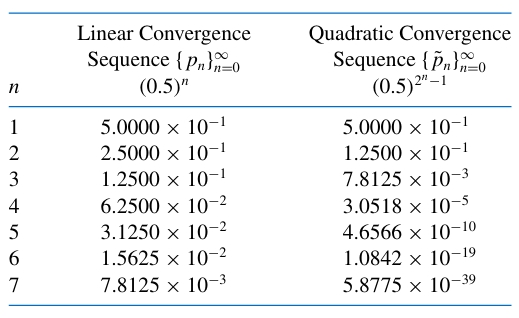
\includegraphics[ width=9cm]{Erroranalysisiterativemethods.jpeg}
\caption{\scriptsize Table 1}
\label{mod2tab1}
\end{table}

Quadratically convergent sequences are expected to converge much quicker than those that converge only linearly, but the next result implies that an arbitrary technique that  generates a convergent sequence does so only linearly.

\begin{theorem}\label{erroranalysisthm1}
Let $g\in C[a,b]$ be such that $g(x)\in[a,b]$, for all $x\in[a,b]$. Suppose, in addition, that $g$ is  continuous on $(a,b)$ and a positive constant $k<1$ exists with
\[|g'(x)|\leq k,\quad\mbox{for all } x\in(a,b).\]
If $g'(p)\neq0$, then for any number $p_0=p$ in $[a,b]$, the sequence
\[p_n=g(p_{n-1}),\quad\mbox{for } n\geq1,\]
converges only linearly to the unique fixed point $p$ in $[a,b]$.
\end{theorem}

Theorem \ref{erroranalysisthm1} implies that higher-order convergence for fixed-point methods of the form $ g(p) = p$ can occur only when $g(p) = 0$. The next result describes additional conditions that ensure the quadratic convergence we seek.

\begin{theorem}\label{erroranalysisthem2}
Let $p$ be a solution of the equation $x = g(x)$. Suppose that $g'(p) = 0$ and $g''$ is continuous with $|g(x)|<M$ on an open interval I containing $p$. Then there exists a $\delta>0$ such that, for $p_0\in[p-\delta, p+\delta]$, the sequence defined by $p_n = g(p_{n-1})$, when $n\geq1$, converges at least quadratically to $p$.  Moreover, for sufficiently large values of $n$,
\[|p_{n+1}-p|<\frac{M}{2}|p_n-p|^2.\]
\end{theorem}
Theorems \ref{erroranalysisthm1} and 2 tell us that our search for quadratically convergent fixed-point methods should point in the direction of functions whose derivatives are zero at the fixed
 point. That is:
\begin{boxB} 
For a fixed point method to converge quadratically we need to have both $g(p) = p$, and $g(p) = 0$.
\end{boxB}

The easiest way to construct a fixed-point problem associated with a root-finding problem $f(x) = 0$ is to add or subtract a multiple of $f(x)$ from $x$. Consider the sequence
\[p_n=g(p_{n-1}),\quad \mbox{for} n\leq1,\]
for $g$ in the form
\[g(x)=x-\phi(x)f(x),\]
 where $\phi$ is a differentiable function that will be chosen later.

For the iterative procedure derived from g to be quadratically convergent, we need to have $g(p) = 0$ when $f(p) = 0$. Because
\[g'(x)=1-\phi'(x)f(x)-f'(x)\phi(x),\]
and $f(p)=0$, we have
\[g'(p)=1-\phi'(p)f(p)-f'(p)\phi(p)=1-\phi'(p)\cdot0-f'(p)\phi(p)=1-f'(p)\phi(p),\]
and $g'(p)=0$ if and only if $\phi(p)=1/f'(p)$.

If we let $\phi(x) = 1/f' (x)$, then we will ensure that $\phi(p) = 1/f'(p)$ and produce the quadratically convergent procedure
\[p_n = g(p_{n-1}) =p_{n-1}-\frac{f(p_{n-1})}{f'(p_{n-1})}.\]
This, of course, is simply Newton’s method. Hence
\begin{boxB} 
If $f(p) = 0$ and $f'(p)= 0$, then for starting values sufficiently close to $p$, Newton’s method will converge at least quadratically.
\end{boxB} 

\subsection*{ Multiple Roots}
In the preceding discussion, the restriction was made that $f'(p)= 0$, where $p$ is the solution to $f(x) = 0$. In particular, Newton’s method and the Secant method will generally give problems if $f'(p) = 0$ when $f(p) = 0$. To examine these difficulties in more detail, we make the following definition.

\begin{definition}
A solution $p$ of $f(x) = 0$ is a {\bf zero of multiplicity} $m$ of $f$ if for $x= p$, we can write $f(x) = (x-p)^mq(x)$, where $lim_{x\rightarrow p}q(x)= 0$.
\end{definition}
In essence, $q(x)$ represents that portion of $f(x)$ that does not contribute to the zero of $f$. The following result gives a means to easily identify {\bf simple} zeros of a function, those that have multiplicity one.

\begin{theorem}\label{erroranalysisthm3}
The function $f\in  C^1[a,b]$ has a simple zero at $p$ in $(a,b)$ if and only if $f(p) = 0$, but $f'(p)= 0$.
\end{theorem}
 The following a generalization of Theorem \ref{erroranalysisthm3}.
\begin{theorem}\label{erroranalysisthm4}

The function $f\in C^m[a,b]$ has a zero of multiplicity $m$ at $p$ in $(a,b)$ if and only if 
\[0=f(p)=f'(p)=f'' (p)=\cdots=f^{(m-1)}(p), \quad\mbox{but}\quad f^{(m)}(p)\neq0.\]
\end{theorem}

The result in Theorem \ref{erroranalysisthm4} implies that an interval about $p$ exists where Newton’s  method converges quadratically to $p$ for any initial approximation $p_0=p$, provided that $p$ is a simple zero. The following example shows that quadratic convergence might not occur if the zero is not simple.

\begin{example}\label{erroranalysisexample1}
Let $f(x)=e^x−x−1$. (a) Show that $f$ has a zero of multiplicity $2$ at $x=0$. (b) Show that  Newton’s method with $p_0=1$ converges to this zero but not quadratically.
\end{example}

\begin{mysolution}
\begin{enumerate}[label=(\alph*)]
\item We have
\[f(x)=e^x−x−1,\qquad f'(x)=e^x−1\qquad \mbox{and}\qquad f''(x)=e^x,\]
so
\[f(0)=e^0−0−1=0,\qquad f'(0)=e^0−1=0 \qquad\mbox{and}\qquad f''(0)=e^0=1.\] 
Theorem \ref{erroranalysisthm4} implies that $f$ has a zero of multiplicity $2$ at $x=0$.
\item The first two terms generated by Newton’s method applied to $f$ with $p_0=1$ are
\[p_1=p_0-\frac{f(p0)}{f'(p_0)} =1-\frac{e-2}{e-1}\approx0.58198,\]
and
\[p_2=p_1-\frac{f(p_1)}{f'(p_1)}\approx0.58198-\frac{0.20760}{0.78957}\approx0.31906.\]
The first sixteen terms of the sequence generated by Newton’s method are shown in Table \ref{table2}. The sequence is clearly converging to $0$, but not quadratically. The graph of $f$ is shown in Figure \ref{pic1}.
\end{enumerate}
\end{mysolution}

\begin{table}[h]
\centering
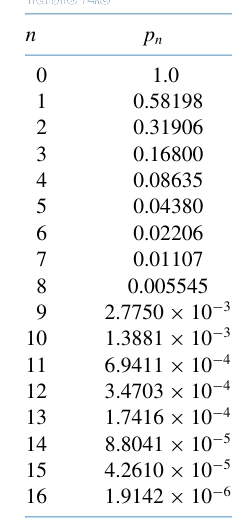
\includegraphics[ width=4cm]{erroranalysistable2.jpeg}
\caption{\scriptsize Table $2$}
\label{table2}
\end{table}

\begin{figure}[h]
\centering
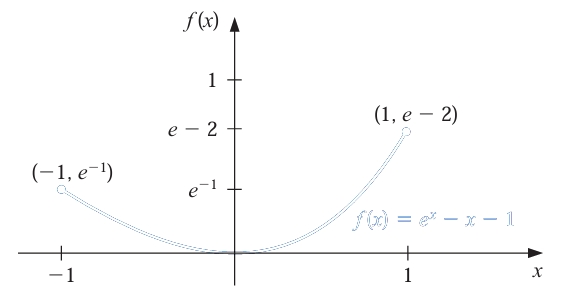
\includegraphics[ width=9cm]{erroranalysispic1.jpeg}
\caption{\scriptsize Figure $1$}
\label{pic1}
\end{figure}

One method of handling the problem of multiple roots of a function $f$ is to define
\[\mu(x)=\frac{f(x)}{f'(x)}.\]
If $p$ is a zero of $f$ of multiplicity $m$ with $f(x)=(x−p)^mq(x)$, then
\[\begin{split}
\mu(x)&=\frac{(x-p)^mq(x)}{m(x-p)^{m-1}q(x)+(x-p)^mq'(x)}\\
 &=(x-p)\frac{q(x)}{mq(x)+(x-p)q'(x)}
\end{split}\]
also has a zero at $p$. However, $q(p)\neq0$, so
\[\frac{q(p)}{mq(p)+(p-p)q'(p)} =\frac1m\neq0,\]
and $p$ is a simple zero of $\mu(x)$. Newton’s method can then be applied to $\mu(x)$ to give
\[g(x)=x-\frac{\mu(x)}{\mu'(x)} =x-\frac{f(x)/f(x)}{\{[f'(x)]^2-[f(x)][f''(x)]\}/[f'(x)]2}\]
which simplifies to
\begin{equation}\label{erroranalysiseqn1}
g(x)=x-\frac{f(x)f'(x)}{[f'(x)]^2-f(x)f''(x)}.
\end{equation}

If $g$ has the required continuity conditions, functional iteration applied to $g$ will be  quadratically convergent regardless of the multiplicity of the zero of $f$. Theoretically, the  only draw back to this method is the additional calculation of $f(x)$ and the more laborious procedure of calculating the iterates. In practice, however, multiple roots can cause serious round-off problems because the denominator of \ref{erroranalysiseqn1} consists of the difference of two numbers that are both close to $0$.


erroranalysisexample1
\begin{example}
In Example \ref{erroranalysisexample1} it was shown that $f(x)=e^x-x-1$ has a zero of multiplicity $2$ at $x=0$ and that Newton’s method with $p_0=1$ converges to this zero but not quadratically. Showt hat the  modification of Newton’s method as given in Equation \ref{erroranalysiseqn1} improves the rate of convergence.
\end{example}

\begin{mysolution}
Modified Newton’s method gives
\[\begin{split}
p_1&=p_0-\frac{f(p_0)f'(p_0)}{f'(p_0)^2-f(p_0)f''(p_0)} \\
&=1-\frac{(e-2)(e-1)}{(e-1)^2-(e-2)e}\approx-2.3421061\times10^{-1}.
\end{split}\]
This is considerably closer to $0$ than the first term using Newton’s method, which was $0.58918$. Table\ref{table3} lists the first five approximations to the double zero at $x=0$. The results were obtained using a system with ten digits of precision. The relative lack of improvement in the last two entries is due to the fact that using this system both the numerator and the denominator approach $0$. Consequently there is a loss of significant digits of accuracy as the approximations approach $0$.
\end{mysolution}

\begin{table}
\centering
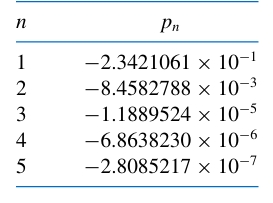
\includegraphics[ width=5cm]{Erroanalysisexampletable3.jpeg}
\caption{\scriptsize Table $3$}
\label{table3}
\end{table}


The following illustrates that the modified Newton’s method converges quadratically  even when in the case of a simple zero.
\begin{example}
In Section $4$ of Module $1$ we found that a zero of $f(x)=x^3+4x^2-10=0$ is $p=1.36523001$. Here we will compare convergence for a simple zero using both Newton’s method and the modified Newton’s method listed in Eq.\ref{erroranalysiseqn1}. Let
\begin{enumerate}[label=(\roman*)]
\item $\displaystyle p_n = p_{n-1}-\frac{p^3_{n-1}+4p^2_{n-1}-10}{3p^2_{n-1}+ 8p_{n-1}}$, from Newton’s method and, from the Modified Newton’s method given by Eq. \ref{erroranalysiseqn1},
\item $\displaystyle p_n = p_{n-1}-\frac{\left(p^3_{n-1}+4p^2_{n-1}-10\right)\left(3p^2_{n-1}+8p_{n-1}\right)}{\left(3p^2_{n-1}+8p_{n-1}\right)^2-\left(p^3_{n-1}+4p^2_{n-1}-10\right)\left(6p_{n-1}+8\right)}$.

With $p_0 = 1.5$, we have
\begin{itemize}
\item[] {\bf Newton's method}
\[ p_1=1.37333333,\quad p_2 = 1.36526201,\quad \mbox{and}\quad p_3 = 1.36523001.\]
\item[] {\bf Modified Newton's method}
\[p_1 = 1.35689898,\quad p_2 = 1.36519585,\quad \mbox{and}\quad p_3 = 1.36523001.\]
\end{itemize}
Both methods are rapidly convergent to the actual zero, which is given by both methods as $p_3$. Note, however, that in the case of a simple zero the original Newton’s method requires substantially less computation.
\end{enumerate}
\end{example}

\begin{myexercise}%\label{Comprehensionquiz2}
Use Newton’s method to find solutions accurate to within $10^{-5}$ to the following problems.
\begin{enumerate}[label=(\alph*)]
\item $x^2 -2xe^{-x} +e^{-2x} = 0$, for $0\leq x \leq1$
\item  $\cos(x + \sqrt{2})+x(x/2+\sqrt{2}) = 0$, for $-2 \leq x \leq-1$
\item $x^3 -3x^2(2^{-x}) + 3x(4^{-x}) - 8^{-x} = 0$, for $0 \leq x \leq 1$
\item $e^{6x} + 3(\ln2)^2e^{2x} - (\ln8)e^{4x} - (\ln2)^3 = 0$, for $-1 \leq x \leq 0$
\end{enumerate}
\begin{mysolution}
\begin{enumerate}[label=(\alph*)]
\item For $p_0=0.5$, we have $p_{13}=0.567135$.
\item For $p_0=-1.5$, we have $p_{23}=-1.414325$.
\item For $p_0=0.5$, we have $p_{22}=0.641166$
\item For$p_0=-0.5$, we have $p_{23}=-0.183274$
\end{enumerate}
\end{mysolution}
\end{myexercise}

\section{Accelerating Convergence}

\begin{youtube}
This video presents a discussion on techniques of accelerating convergence in iterative processes. Follow the discussion and then solve the problems in the subsequent quiz.
\mylink{https://www.youtube.com/watch?v=RYsva1tesvg}
\end{youtube}


\begin{myexercise}%\label{Comprehensionquiz2}
The following sequences are linearly convergent. Generate the first five terms of the sequence $\left\{q_{n}\right\}$ using Aitken's $\Delta^{2}$ method.
\begin{enumerate}[label=(\alph*)]
\item$p_{0}=0.5, \quad p_{n}=\left(2-e^{p_{n-1}}+p_{n-1}^{2}\right) / 3, \quad$ for $n \geq 1$
\item $p_{0}=0.75, \quad p_{n}=\left(e^{p_{n-1}} / 3\right)^{1 / 2}, \quad$ for $n \geq 1$
\item $p_{0}=0.5, \quad p_{n}=3^{-p_{n-1}}, \quad$ for $n \geq 1$
\item $p_{0}=0.5, \quad p_{n}=\cos p_{n-1}, \quad$ for $n \geq 1$ 
\end{enumerate}
\begin{mysolution}
The results are listed in the following table

\begin{center}
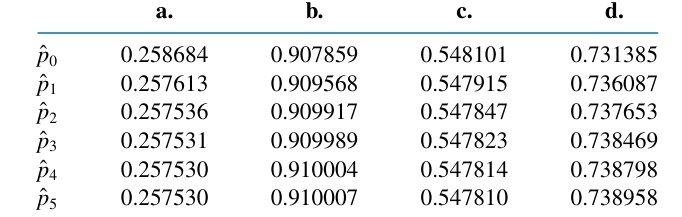
\includegraphics[width=13cm]{Mod2Sec2Comquiz}
\end{center}
\end{mysolution}
\end{myexercise}



\section{Zeroes of Polynomials and M\"uller's Method}
%\activities
%Read on zeros of polynomials and M\"uller's method in pages \textcolor{red}{\bf page $93-100$} of the following reference and then attempt the subsequent quiz
%\begin{activity}[\cg Reading]
%\begin{enumerate}
%\item Burden, R. L., Faires, J. D., Burden, A. M. (2015). Numerical Analysis. Tenth Edition, Cengage Learning.\\
%\end{enumerate}
%\end{activity}

\begin{youtube}
This video presents a discussion on zeros of polynomials and \\M\"uller's method. Follow the discussion and then solve the\\ problems in the subsequent quiz.\\
\mylink{https://www.youtube.com/watch?v=PcGGwhV8PvE\&t=24s}
\end{youtube}



\begin{myexercise}%\label{Comprehensionquiz2}
Find the approximations to within $10^{-4}$ to all the real zeros of the following polynomials using Newton's method.
\begin{enumerate}[label=(\alph*)]
\item $P(x)=x^{3}-2 x^{2}-5$
\item $P(x)=x^{3}+3 x^{2}-1$
\item $P(x)=x^{3}- x-1$
\item $P(x)=x^{4}+2 x^{2}-x-3$
\item $P(x)=x^{3}+4.001 x^{2}+4.002x+1.101$
\item $P(x)=x^{5}-x^{4}+2 x^{3}-3 x^{2}+x-4$
\end{enumerate}
\begin{mysolution}
\begin{enumerate}[label=(\alph*)]
\item For $p_0=1$, we have $p_{22}=2.69065$.
\item For $p_0=1$, we have $p_5=0.53209$; for $p_0=-1$, we have $p_3=-0.65270$; and for $p_0=-3$, we have $p_3=-2.87939$.
\item For $p_0=1$, we have $p_5=1.32472$.
\item For $p_0=1$, we have $p_4=1.12412$; and for $p_0=0$, we have $p_8=-0.87605$.
\item For $p_0=0$, we have $p_6=-0.47006$; for $p_0=-1$, we have $p_4=-0.88533$; and for $p_0=-3$, we have $p_4=-2.64561$.
\item For $p_0=0$, we have $p_{10}=1.49819$.
\end{enumerate}
\end{mysolution}
\end{myexercise}


\section{Interpolation and the Lagrange Polynomial}
\videolesson
\begin{selfvideo}[2]
%LESSON 3: 
This video presents a discussion on interpolation and the Lagrange polynomial. Follow the discussion and then solve the problems in the subsequent quiz.
\end{selfvideo}
%\begin{boxB}Question: \end{boxB}

One of the most useful and well-known classes of functions mapping the set of real numbers into itself is the algebraic polynomials, the set of functions of the form
\[P_{n}(x)=a_{n} x^{n}+a_{n-1} x^{n-1}+\cdots+a_{1} x+a_{0},\]
where $n$ is a nonnegative integer and $a_{0}, \ldots, a_{n}$ are real constants. One reason for their importance is that they uniformly approximate continuous functions. By this we mean that given any function, defined and continuous on a closed and bounded interval, there exists a polynomial that is as ``close'' to the given function as desired. This result is expressed precisely in the Weierstrass Approximation Theorem. (See Figure \ref{Interpolandlagrfig1}.)

\begin{figure}[h]
\centering
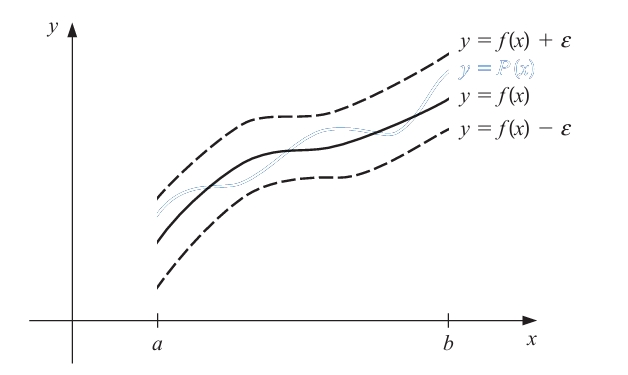
\includegraphics[ width=10cm]{InterpolandLagrfig1.jpeg}
\caption{\scriptsize Figure $2$}
\label{Interpolandlagrfig1}
\end{figure}

\begin{theorem}[Weierstrass Approximation Theorem]
Suppose that $f$ is defined and continuous on $[a, b]$. For each $\epsilon>0$, there exists a polynomial $P(x)$, with the property that
\[|f(x)-P(x)|<\epsilon, \quad \text { for all } x \text { in }[a, b].\]
\end{theorem}
One important reason for considering the class of polynomials in the approximation of functions is that the derivative and indefinite integral of a polynomial are easy to determine and are also polynomials. For these reasons, polynomials are often used for approximating continuous functions.

A class of polynomials that can be considered is the Taylor polynomials which agree as closely as possible with a given function at a specific point, but they concentrate their accuracy near that point. A good interpolation polynomial needs to provide a relatively accurate approximation over an entire interval, and Taylor polynomials do not generally do this. 
%For example, suppose we calculate the first six Taylor polynomials about $x_{0}=0$ for $f(x)=e^{x}$. Since the derivatives of $f(x)$ are all $e^{x}$, which evaluated at $x_{0}=0$ gives 1 , the Taylor polynomials are
%
%Very little of Weierstrass's work was published during his lifetime, but his lectures, particularly on the theory of functions, had significant influence on an entire generation of students.
%
%$$
%\begin{aligned}
%& P_{0}(x)=1, \quad P_{1}(x)=1+x, \quad P_{2}(x)=1+x+\frac{x^{2}}{2}, \quad P_{3}(x)=1+x+\frac{x^{2}}{2}+\frac{x^{3}}{6}, \\
%& P_{4}(x)=1+x+\frac{x^{2}}{2}+\frac{x^{3}}{6}+\frac{x^{4}}{24}, \quad \text { and } \quad P_{5}(x)=1+x+\frac{x^{2}}{2}+\frac{x^{3}}{6}+\frac{x^{4}}{24}+\frac{x^{5}}{120} .
%\end{aligned}
%$$
%
%The graphs of the polynomials are shown in Figure 3.2. (Notice that even for the higher-degree polynomials, the error becomes progressively worse as we move away from zero.)
%
%Figure 3.2\\
%\includegraphics[max width=\textwidth, center]{2025_05_15_4109a88b43049bd640d1g-03}
%
%Although better approximations are obtained for $f(x)=e^{x}$ if higher-degree Taylor polynomials are used, this is not true for all functions. Consider, as an extreme example, using Taylor polynomials of various degrees for $f(x)=1 / x$ expanded about $x_{0}=1$ to approximate $f(3)=1 / 3$. Since
%
%$$
%f(x)=x^{-1}, f^{\prime}(x)=-x^{-2}, f^{\prime \prime}(x)=(-1)^{2} 2 \cdot x^{-3}
%$$
%
%and, in general,
%
%$$
%f^{(k)}(x)=(-1)^{k} k!x^{-k-1}
%$$
%
%the Taylor polynomials are
%
%$$
%P_{n}(x)=\sum_{k=0}^{n} \frac{f^{(k)}(1)}{k!}(x-1)^{k}=\sum_{k=0}^{n}(-1)^{k}(x-1)^{k}
%$$
%
%To approximate $f(3)=1 / 3$ by $P_{n}(3)$ for increasing values of $n$, we obtain the values in Table 3.1-rather a dramatic failure! When we approximate $f(3)=1 / 3$ by $P_{n}(3)$ for larger values of $n$, the approximations become increasingly inaccurate.
%
%Table 3.1
%
%\begin{center}
%\begin{tabular}{c|c|c|c|c|c|c|c|c}
%$n$ & 0 & 1 & 2 & 3 & 4 & 5 & 6 & 7 \\
%\hline
%$P_{n}(3)$ & 1 & -1 & 3 & -5 & 11 & -21 & 43 & -85 \\
%\hline
%\end{tabular}
%\end{center}
%
%For the Taylor polynomials all the information used in the approximation is concentrated at the single number $x_{0}$, so these polynomials will generally give inaccurate approximations as we move away from $x_{0}$. This limits Taylor polynomial approximation to the situation in which approximations are needed only at numbers close to $x_{0}$. For ordinary computational purposes it is more efficient to use methods that include information at various points. We consider this in the remainder of the chapter. 
The primary use of Taylor polynomials in numerical analysis is not for approximation purposes, but for the derivation of numerical techniques and error estimation.

\subsection*{Lagrange Interpolating Polynomials}
The problem of determining a polynomial of degree one that passes through the distinct points $\left(x_{0}, y_{0}\right)$ and $\left(x_{1}, y_{1}\right)$ is the same as approximating a function $f$ for which $f\left(x_{0}\right)=y_{0}$ and $f\left(x_{1}\right)=y_{1}$ by means of a first-degree polynomial {\bf interpolating}, or agreeing with, the values of $f$ at the given points. Using this polynomial for approximation within the interval given by the endpoints is called polynomial {\bf interpolation}.

Define the functions
\[L_{0}(x)=\frac{x-x_{1}}{x_{0}-x_{1}} \quad \text { and } \quad L_{1}(x)=\frac{x-x_{0}}{x_{1}-x_{0}}\]
The linear {\bf Lagrange interpolating polynomial through} ( $x_{0}, y_{0}$ ) and ( $x_{1}, y_{1}$ ) is
\[P(x)=L_{0}(x) f\left(x_{0}\right)+L_{1}(x) f\left(x_{1}\right)=\frac{x-x_{1}}{x_{0}-x_{1}} f\left(x_{0}\right)+\frac{x-x_{0}}{x_{1}-x_{0}} f\left(x_{1}\right).\]
Note that
\[L_{0}\left(x_{0}\right)=1, \quad L_{0}\left(x_{1}\right)=0, \quad L_{1}\left(x_{0}\right)=0, \quad \text { and } \quad L_{1}\left(x_{1}\right)=1,\]
which implies that
\[P\left(x_{0}\right)=1 \cdot f\left(x_{0}\right)+0 \cdot f\left(x_{1}\right)=f\left(x_{0}\right)=y_{0}\]
and
\[P\left(x_{1}\right)=0 \cdot f\left(x_{0}\right)+1 \cdot f\left(x_{1}\right)=f\left(x_{1}\right)=y_{1}\]
So $P$ is the unique polynomial of degree at most one that passes through ( $x_{0}, y_{0}$ ) and $\left(x_{1}, y_{1}\right)$.

\begin{example}
Determine the linear Lagrange interpolating polynomial that passes through the points $(2,4)$ and $(5,1)$.
\end{example}

\begin{mysolution} 
In this case we have
\[L_{0}(x)=\frac{x-5}{2-5}=-\frac{1}{3}(x-5) \quad \text { and } \quad L_{1}(x)=\frac{x-2}{5-2}=\frac{1}{3}(x-2)\]
so
\[P(x)=-\frac{1}{3}(x-5) \cdot 4+\frac{1}{3}(x-2) \cdot 1=-\frac{4}{3} x+\frac{20}{3}+\frac{1}{3} x-\frac{2}{3}=-x+6\]
The graph of $y=P(x)$ is shown in Figure \ref{Lagrangepolynoexample1}.
\end{mysolution}

\begin{figure}[h]
\centering
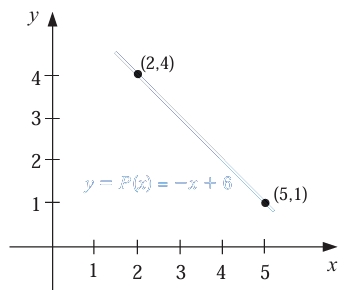
\includegraphics[ width=7cm]{Lagrangepolyexample1.jpeg}
\caption{\scriptsize Figure $3$}
\label{Lagrangepolynoexample1}
\end{figure}

To generalize the concept of linear interpolation, consider the construction of a polynomial of degree at most $n$ that passes through the $n+1$ points
\[\left(x_{0}, f\left(x_{0}\right)\right),\left(x_{1}, f\left(x_{1}\right)\right), \ldots,\left(x_{n}, f\left(x_{n}\right)\right).\]
(See Figure \ref{Lagrangepolynoexplainfig1}.)

\begin{figure}[h]
\centering
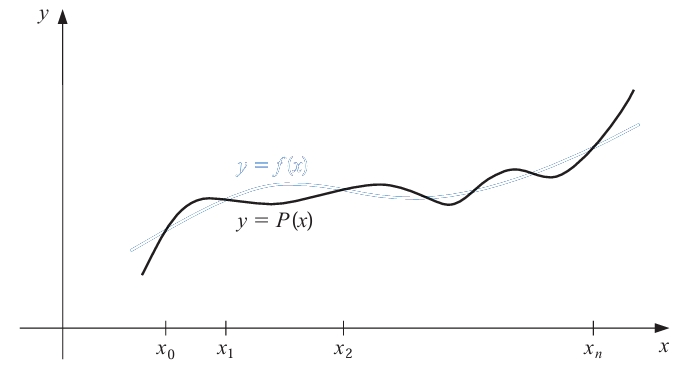
\includegraphics[ width=12cm]{Lagrangepolyexplainfig1.jpeg}
\caption{\scriptsize Figure $4$}
\label{Lagrangepolynoexplainfig1}
\end{figure}

In this case we first construct, for each $k=0,1, \ldots, n$, a function $L_{n, k}(x)$ with the property that $L_{n, k}\left(x_{i}\right)=0$ when $i \neq k$ and $L_{n, k}\left(x_{k}\right)=1$. To satisfy $L_{n, k}\left(x_{i}\right)=0$ for each $i \neq k$ requires that the numerator of $L_{n, k}(x)$ contain the term
\[\left(x-x_{0}\right)\left(x-x_{1}\right) \cdots\left(x-x_{k-1}\right)\left(x-x_{k+1}\right) \cdots\left(x-x_{n}\right).\]
To satisfy $L_{n, k}\left(x_{k}\right)=1$, the denominator of $L_{n, k}(x)$ must be this same term but evaluated at $x=x_{k}$.
Thus
\[L_{n, k}(x)=\frac{\left(x-x_{0}\right) \cdots\left(x-x_{k-1}\right)\left(x-x_{k+1}\right) \cdots\left(x-x_{n}\right)}{\left(x_{k}-x_{0}\right) \cdots\left(x_{k}-x_{k-1}\right)\left(x_{k}-x_{k+1}\right) \cdots\left(x_{k}-x_{n}\right)}.\]
A sketch of the graph of a typical $L_{n, k}$ (when $n$ is even) is shown in Figure \ref{Lagrangepolynoexplainfig2}.

\begin{figure}
\centering
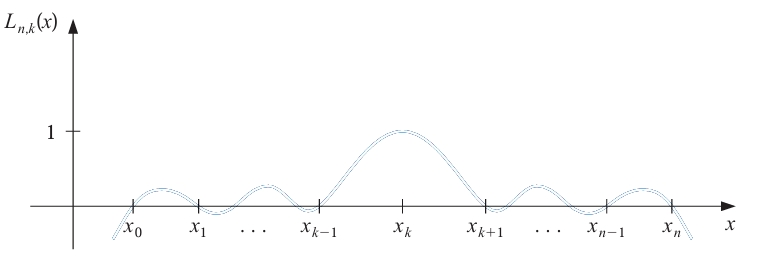
\includegraphics[ width=14cm]{Lagrangepolyexplainfig2.jpeg}
\caption{\scriptsize Figure $5$}
\label{Lagrangepolynoexplainfig2}
\end{figure}

The interpolating polynomial is easily described once the form of $L_{n, k}$ is known. This polynomial, called the $\boldsymbol{n}$ th Lagrange interpolating polynomial, is defined in the following theorem.

\begin{theorem}\label{langrainterpolthm1}
%The interpolation formula named for Joseph Louis Lagrange (1736-1813) was likely known by Isaac Newton around 1675, but it appears to first have been published in 1779 by Edward Waring (1736-1798). Lagrange wrote extensively on the subject of interpolation and his work had significant influence on later mathematicians. He published this result in 1795.
%
%The symbol $\prod$ is used to write products compactly and parallels the symbol $\sum$, which is used for writing sums.
%
If $x_{0}, x_{1}, \ldots, x_{n}$ are $n+1$ distinct numbers and $f$ is a function whose values are given at these numbers, then a unique polynomial $P(x)$ of degree at most $n$ exists with
\[f\left(x_{k}\right)=P\left(x_{k}\right), \quad \text { for each } k=0,1, \ldots, n.\]
This polynomial is given by
\begin{equation}\label{Lagrangepolyexplaineq1}
P(x)=f\left(x_{0}\right) L_{n, 0}(x)+\cdots+f\left(x_{n}\right) L_{n, n}(x)=\sum_{k=0}^{n} f\left(x_{k}\right) L_{n, k}(x), \end{equation}
where, for each $k=0,1, \ldots, n$,
\begin{equation}\label{Lagrangepolyexplaineq2}
\begin{split}
L_{n, k}(x) & =\frac{\left(x-x_{0}\right)\left(x-x_{1}\right) \cdots\left(x-x_{k-1}\right)\left(x-x_{k+1}\right) \cdots\left(x-x_{n}\right)}{\left(x_{k}-x_{0}\right)\left(x_{k}-x_{1}\right) \cdots\left(x_{k}-x_{k-1}\right)\left(x_{k}-x_{k+1}\right) \cdots\left(x_{k}-x_{n}\right)} \\
& =\prod_{\substack{i=0 \\i \neq k}}^{n} \frac{\left(x-x_{i}\right)}{\left(x_{k}-x_{i}\right)}
\end{split}
\end{equation}
\end{theorem}
We will write $L_{n, k}(x)$ simply as $L_{k}(x)$ when there is no confusion as to its degree.

\begin{example}
\begin{enumerate}[label=(\alph*)]
\item Use the numbers (called nodes) $x_{0}=2, x_{1}=2.75$, and $x_{2}=4$ to find the second Lagrange interpolating polynomial for $f(x)=1 / x$.
\item Use this polynomial to approximate $f(3)=1 / 3$.
\end{enumerate}
\end{example}

\begin{mysolution} 
\begin{enumerate}[label=(\alph*)]
\item We first determine the coefficient polynomials $L_{0}(x), L_{1}(x)$, and $L_{2}(x)$. In nested form they are
\[\begin{aligned}
& L_{0}(x)=\frac{(x-2.75)(x-4)}{(2-2.5)(2-4)}=\frac{2}{3}(x-2.75)(x-4) \\
& L_{1}(x)=\frac{(x-2)(x-4)}{(2.75-2)(2.75-4)}=-\frac{16}{15}(x-2)(x-4)
\end{aligned}\]
and
\[L_{2}(x)=\frac{(x-2)(x-2.75)}{(4-2)(4-2.5)}=\frac{2}{5}(x-2)(x-2.75)\]
Also, $f\left(x_{0}\right)=f(2)=1 / 2, f\left(x_{1}\right)=f(2.75)=4 / 11$, and $f\left(x_{2}\right)=f(4)=1 / 4$, so
\[\begin{aligned}
P(x) & =\sum_{k=0}^{2} f\left(x_{k}\right) L_{k}(x) \\
& =\frac{1}{3}(x-2.75)(x-4)-\frac{64}{165}(x-2)(x-4)+\frac{1}{10}(x-2)(x-2.75) \\
& =\frac{1}{22} x^{2}-\frac{35}{88} x+\frac{49}{44}
\end{aligned}\]
\item An approximation to $f(3)=1 / 3$ (see Figure \ref{Lagrangepolynoexample2}) is
\[f(3) \approx P(3)=\frac{9}{22}-\frac{105}{88}+\frac{49}{44}=\frac{29}{88} \approx 0.32955 .\]
%Recall that in the opening section of this chapter (see Table 3.1) we found that no Taylor polynomial expanded about $x_{0}=1$ could be used to reasonably approximate $f(x)=1 / x$ at $x=3$.
\end{enumerate}
\end{mysolution}

\begin{figure}[h]
\centering
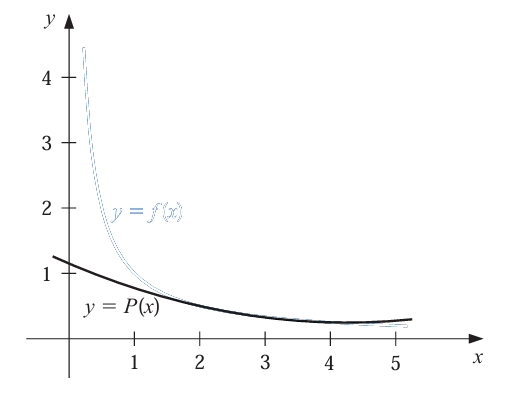
\includegraphics[ width=9cm]{Lagrangepolyexample2.jpeg}
\caption{\scriptsize Figure $6$}
\label{Lagrangepolynoexample2}
\end{figure}

%The interpolating polynomial $P$ of degree less than or equal to 3 is defined in Maple with\\
%$P:=x \rightarrow \operatorname{interp}([2,11 / 4,4],[1 / 2,4 / 11,1 / 4], x)$
%
%$$
%x \rightarrow \operatorname{interp}\left(\left[2, \frac{11}{4}, 4\right],\left[\frac{1}{2}, \frac{4}{11}, \frac{1}{4}\right], x\right)
%$$
%
%To see the polynomial, enter\\
%$P(x)$
%
%$$
%\frac{1}{22} x^{2}-\frac{35}{88} x+\frac{49}{44}
%$$
%
%Evaluating $P(3)$ as an approximation to $f(3)=1 / 3$, is found with evalf( $P(3)$ )
%
%There are other ways that the error term for the Lagrange polynomial can be expressed, but this is the most useful form and the one that most closely agrees with the standard Taylor polynomial error form.
%
%The interpolating polynomial can also be defined in Maple using the CurveFitting package and the call PolynomialInterpolation.
%
The next step is to calculate a remainder term or bound for the error involved in approximating a function by an interpolating polynomial.

\begin{theorem}\label{Lagrangepolyexplaineqthm3}
Suppose $x_{0}, x_{1}, \ldots, x_{n}$ are distinct numbers in the interval $[a, b]$ and $f \in C^{n+1}[a, b]$. Then, for each $x$ in $[a, b]$, a number $\xi(x)$ (generally unknown) between $x_{0}, x_{1}, \ldots, x_{n}$, and hence in ( $a, b$ ), exists with
\begin{equation}
f(x)=P(x)+\frac{f^{(n+1)}(\xi(x))}{(n+1)!}\left(x-x_{0}\right)\left(x-x_{1}\right) \cdots\left(x-x_{n}\right), 
\end{equation}
where $P(x)$ is the interpolating polynomial given in Eq.\ref{Lagrangepolyexplaineq1}.
\end{theorem}
%
%Proof Note first that if $x=x_{k}$, for any $k=0,1, \ldots, n$, then $f\left(x_{k}\right)=P\left(x_{k}\right)$, and choosing $\xi\left(x_{k}\right)$ arbitrarily in ( $a, b$ ) yields Eq. (3.3).
%
%If $x \neq x_{k}$, for all $k=0,1, \ldots, n$, define the function $g$ for $t$ in $[a, b]$ by
%
%$$
%\begin{aligned}
%g(t) & =f(t)-P(t)-[f(x)-P(x)] \frac{\left(t-x_{0}\right)\left(t-x_{1}\right) \cdots\left(t-x_{n}\right)}{\left(x-x_{0}\right)\left(x-x_{1}\right) \cdots\left(x-x_{n}\right)} \\
%& =f(t)-P(t)-[f(x)-P(x)] \prod_{i=0}^{n} \frac{\left(t-x_{i}\right)}{\left(x-x_{i}\right)}
%\end{aligned}
%$$
%
%Since $f \in C^{n+1}[a, b]$, and $P \in C^{\infty}[a, b]$, it follows that $g \in C^{n+1}[a, b]$. For $t=x_{k}$, we have
%
%$$
%g\left(x_{k}\right)=f\left(x_{k}\right)-P\left(x_{k}\right)-[f(x)-P(x)] \prod_{i=0}^{n} \frac{\left(x_{k}-x_{i}\right)}{\left(x-x_{i}\right)}=0-[f(x)-P(x)] \cdot 0=0 .
%$$
%
%Moreover,
%
%$$
%g(x)=f(x)-P(x)-[f(x)-P(x)] \prod_{i=0}^{n} \frac{\left(x-x_{i}\right)}{\left(x-x_{i}\right)}=f(x)-P(x)-[f(x)-P(x)]=0 .
%$$
%
%Thus $g \in C^{n+1}[a, b]$, and $g$ is zero at the $n+2$ distinct numbers $x, x_{0}, x_{1}, \ldots, x_{n}$. By Generalized Rolle's Theorem 1.10, there exists a number $\xi$ in ( $a, b$ ) for which $g^{(n+1)}(\xi)=0$. So
%
%
%\begin{equation*}
%0=g^{(n+1)}(\xi)=f^{(n+1)}(\xi)-P^{(n+1)}(\xi)-[f(x)-P(x)] \frac{d^{n+1}}{d t^{n+1}}\left[\prod_{i=0}^{n} \frac{\left(t-x_{i}\right)}{\left(x-x_{i}\right)}\right]_{t=\xi} \tag{3.4}
%\end{equation*}
%
%
%However $P(x)$ is a polynomial of degree at most $n$, so the $(n+1)$ st derivative, $P^{(n+1)}(x)$, is identically zero. Also, $\prod_{i=0}^{n}\left[\left(t-x_{i}\right) /\left(x-x_{i}\right)\right]$ is a polynomial of degree $(n+1)$, so
%
%$$
%\prod_{i=0}^{n} \frac{\left(t-x_{i}\right)}{\left(x-x_{i}\right)}=\left[\frac{1}{\prod_{i=0}^{n}\left(x-x_{i}\right)}\right] t^{n+1}+(\text { lower-degree terms in } t),
%$$
%
%and
%
%$$
%\frac{d^{n+1}}{d t^{n+1}} \prod_{i=0}^{n} \frac{\left(t-x_{i}\right)}{\left(x-x_{i}\right)}=\frac{(n+1)!}{\prod_{i=0}^{n}\left(x-x_{i}\right)}
%$$
%
%Equation (3.4) now becomes
%
%$$
%0=f^{(n+1)}(\xi)-0-[f(x)-P(x)] \frac{(n+1)!}{\prod_{i=0}^{n}\left(x-x_{i}\right)}
%$$
%
%and, upon solving for $f(x)$, we have
%
%$$
%f(x)=P(x)+\frac{f^{(n+1)}(\xi)}{(n+1)!} \prod_{i=0}^{n}\left(x-x_{i}\right)
%$$

The error formula in Theorem \ref{langrainterpolthm1} is an important theoretical result because Lagrange polynomials are used extensively for deriving numerical differentiation and integration methods. Error bounds for these techniques are obtained from the Lagrange error formula.

Note that the error form for the Lagrange polynomial is quite similar to that for the Taylor polynomial. The $n$th Taylor polynomial about $x_{0}$ concentrates all the known information at $x_{0}$ and has an error term of the form
\[\frac{f^{(n+1)}(\xi(x))}{(n+1)!}\left(x-x_{0}\right)^{n+1}\]
The Lagrange polynomial of degree $n$ uses information at the distinct numbers $x_{0}, x_{1}, \ldots$, $x_{n}$ and, in place of $\left(x-x_{0}\right)^{n}$, its error formula uses a product of the $n+1$ terms $\left(x-x_{0}\right)$, $\left(x-x_{1}\right), \ldots,\left(x-x_{n}\right):$
\[\frac{f^{(n+1)}(\xi(x))}{(n+1)!}\left(x-x_{0}\right)\left(x-x_{1}\right) \cdots\left(x-x_{n}\right)\]

\begin{example}In Example 2 we found the second Lagrange polynomial for $f(x)=1 / x$ on $[2,4]$ using the nodes $x_{0}=2, x_{1}=2.75$, and $x_{2}=4$. Determine the error form for this polynomial, and the maximum error when the polynomial is used to approximate $f(x)$ for $x \varepsilon[2,4]$.
\end{example}

\begin{mysolution}
Because $f(x)=x^{-1}$, we have
\[f^{\prime}(x)=-x^{-2}, \quad f^{\prime \prime}(x)=2 x^{-3}, \quad \text { and } \quad f^{\prime \prime \prime}(x)=-6 x^{-4}.\]
As a consequence, the second Lagrange polynomial has the error form\\
\[\frac{f^{\prime \prime \prime}(\xi(x))}{3!}\left(x-x_{0}\right)\left(x-x_{1}\right)\left(x-x_{2}\right)=-(\xi(x))^{-4}(x-2)(x-2.75)(x-4),\]
for $\xi(x)$ in $(2,4)$. The maximum value of $(\xi(x))^{-4}$ on the interval is $2^{-4}=1 / 16$. We now need to determine the maximum value on this interval of the absolute value of the polynomial
\[g(x)=(x-2)(x-2.75)(x-4)=x^{3}-\frac{35}{4} x^{2}+\frac{49}{2} x-22 .\]
Because
\[D_{x}\left(x^{3}-\frac{35}{4} x^{2}+\frac{49}{2} x-22\right)=3 x^{2}-\frac{35}{2} x+\frac{49}{2}=\frac{1}{2}(3 x-7)(2 x-7),\]
the critical points occur at
\[x=\frac{7}{3}, \text { with } g\left(\frac{7}{3}\right)=\frac{25}{108}, \quad \text { and } \quad x=\frac{7}{2}, \text { with } g\left(\frac{7}{2}\right)=-\frac{9}{16}.\]
Hence, the maximum error is
\[\frac{f^{\prime \prime \prime}(\xi(x))}{3!}\left|\left(x-x_{0}\right)\left(x-x_{1}\right)\left(x-x_{2}\right)\right| \leq \frac{1}{16 \cdot 6}\left|-\frac{9}{16}\right|=\frac{3}{512} \approx 0.00586.\]
\end{mysolution}

The next example illustrates how the error formula can be used to prepare a table of data that will ensure a specified interpolation error within a specified bound.

\begin{example}
Suppose a table is to be prepared for the function $f(x)=e^{x}$, for $x$ in $[0,1]$. Assume the number of decimal places to be given per entry is $d \geq 8$ and that the difference between adjacent $x$-values, the step size, is $h$. What step size $h$ will ensure that linear interpolation gives an absolute error of at most $10^{-6}$ for all $x$ in $[0,1]$ ?
\end{example}

\begin{mysolution}
Let $x_{0}, x_{1}, \ldots$ be the numbers at which $f$ is evaluated, $x$ be in $[0,1]$, and suppose $j$ satisfies $x_{j} \leq x \leq x_{j+1}$. Eq. (3.3) implies that the error in linear interpolation is
\[|f(x)-P(x)|=\left|\frac{f^{(2)}(\xi)}{2!}\left(x-x_{j}\right)\left(x-x_{j+1}\right)\right|=\frac{\left|f^{(2)}(\xi)\right|}{2}\left|\left(x-x_{j}\right)\right|\left|\left(x-x_{j+1}\right)\right|.\]
The step size is $h$, so $x_{j}=j h, x_{j+1}=(j+1) h$, and
\[|f(x)-P(x)| \leq \frac{\left|f^{(2)}(\xi)\right|}{2!}|(x-j h)(x-(j+1) h)|\]
Hence
\[\begin{aligned}
|f(x)-P(x)| & \leq \frac{\max _{\xi \in[0,1]} e^{\xi}}{2} \max _{x_{j} \leq x \leq x_{j+1}}|(x-j h)(x-(j+1) h)| \\
& \leq \frac{e}{2} \max _{x_{j} \leq x \leq x_{j+1}}|(x-j h)(x-(j+1) h)|
\end{aligned}\]

Consider the function $g(x)=(x-j h)(x-(j+1) h)$, for $j h \leq x \leq(j+1) h$. Because
\[g^{\prime}(x)=(x-(j+1) h)+(x-j h)=2\left(x-j h-\frac{h}{2}\right),\]
the only critical point for $g$ is at $x=j h+h / 2$, with $g(j h+h / 2)=(h / 2)^{2}=h^{2} / 4$.

Since $g(j h)=0$ and $g((j+1) h)=0$, the maximum value of $\left|g^{\prime}(x)\right|$ in $[j h,(j+1) h]$ must occur at the critical point which implies that
\[|f(x)-P(x)| \leq \frac{e}{2} \max _{x_{j} \leq x \leq x_{j+1}}|g(x)| \leq \frac{e}{2} \cdot \frac{h^{2}}{4}=\frac{e h^{2}}{8}.\]
Consequently, to ensure that the the error in linear interpolation is bounded by $10^{-6}$, it is sufficient for $h$ to be chosen so that
\[\frac{e h^{2}}{8} \leq 10^{-6}. \text { This implies that } h<1.72 \times 10^{-3}.\]
Because $n=(1-0) / h$ must be an integer, a reasonable choice for the step size is $h=0.001$.
\end{mysolution}
\begin{myexercise}%\label{Comprehensionquiz2}
For the given functions $f(x)$, let $x_{0}=0, x_{1}=0.6$, and $x_{2}=0.9$. Construct interpolation polynomials of degree at most one and at most two to approximate $f(0.45)$, and find the absolute error.
\begin{multicols}{2}
\begin{enumerate}[label=(\alph*)]
\item $f(x)=\cos x$
\item $f(x)=\sqrt{1+x}$
\item $\quad f(x)=\ln (x+1)$
\item $f(x)=\tan x$
\end{enumerate}
\end{multicols}

\begin{mysolution}
\begin{enumerate}[label=(\alph*)]
\item $P_1(x)=-0.148878x+1$; $P_2(x)=-0.452592x^2-0.0131009x+1$; $P_1(0.45)=0.933005$;
 $|f(0.45)-P_1(0.45)|=0.032558$; $P_2(0.45)=0.902455$; $|f(0.45)-P_2(0.45)|=0.002008$
\item $P_1(x)=0.467251x+1$; $P_2(x)=-0.0780026x^2+0.490652x+1$; $P_1(0.45)=1.210263$;
 $|f(0.45)-P_1(0.45)|=0.006104$; $P_2(0.45)=1.204998$; $|f(0.45)-P_2(0.45)|=0.000839$
\item $P_1(x)=0.874548x$; $P_2(x)=-0.268961x^2+0.955236x$; $P_1(0.45)=0.393546$; $|f(0.45)-P_1(0.45)|=0.0212983$; $P_2(0.45)=0.375392$; $|f(0.45)-P_2(0.45)|=0.003828$
\item $P_1(x)=1.031121x$; $P_2(x)=0.615092x^2+0.846593x$; $P_1(0.45)=0.464004$; $|f(0.45)-P1(0.45)|=0.019051$; $P_2(0.45)=0.505523$; $|f(0.45)-P2(0.45)|=0.022468$
\end{enumerate}
\end{mysolution}
\end{myexercise}


%\discussion


\begin{posttest}[\textcolor{red}{End of Module 2 Quiz}]
\item Use the modified Newton’s method given as 
\[g(x)=x-\frac{f(x)f'(x)}{{[f'(x)]^2-[f(x)][f''(x)]}/[f'(x)]^2}\]
to find solutions accurate to within $10^{-5}$ to the following problems. Is there an improve
ment in speed or accuracy over Comprehension Quiz for section $1$?
\begin{enumerate}[label=(\alph*)]
\item $x^2 -2xe^{-x} +e^{-2x} = 0$, for $0\leq x \leq1$
\item  $\cos(x + \sqrt{2})+x(x/2+\sqrt{2}) = 0$, for $-2 \leq x \leq-1$
\item $x^3 -3x^2(2^{-x}) + 3x(4^{-x}) - 8^{-x} = 0$, for $0 \leq x \leq 1$
\item $e^{6x} + 3(\ln2)^2e^{2x} - (\ln8)e^{4x} - (\ln2)^3 = 0$, for $-1 \leq x \leq 0$
\end{enumerate}
\item Let $g(x) = \cos(x -1)$ and $p^{(0)}_0 =2$. Use Steffensen’s method to find $p^{(1)}_0$.
\item Find the approximations to within $10^{-4}$ to all the real zeros of the following polynomials using M\''uler's method.
\begin{enumerate}[label=(\alph*)]
\item $P(x)=x^{3}-2 x^{2}-5$
\item $P(x)=x^{3}+3 x^{2}-1$
\item $P(x)=x^{3}- x-1$
\item $P(x)=x^{4}+2 x^{2}-x-3$
\item $P(x)=x^{3}+4.001 x^{2}+4.002x+1.101$
\item $P(x)=x^{5}-x^{4}+2 x^{3}-3 x^{2}+x-4$
\end{enumerate}
\item Use Theorem \ref{Lagrangepolyexplaineqthm3} to find an error bound for the approximations in the Comprehension Quiz for Section $4$.
\begin{mysolution}
\begin{enumerate}[label=\arabic*.]
\item
\begin{enumerate}[label=(\alph*)]
\item For $p_0=0.5$, we have $p_{3}=0.567143$.
\item For $p_0=-1.5$, we have $p_{2}=-1.414158$
\item For $p_0=0.5$, we have $p_3=0.641274$.
\item For$p_0=-0.5$, we have $p_5=-0.183319$.
\end{enumerate}
These figures show an improvement in speed and accuracy.
\item $p^{(1)}_0 =0.826427$
\item The following table lists the initial approximation and the roots.
\begin{center}
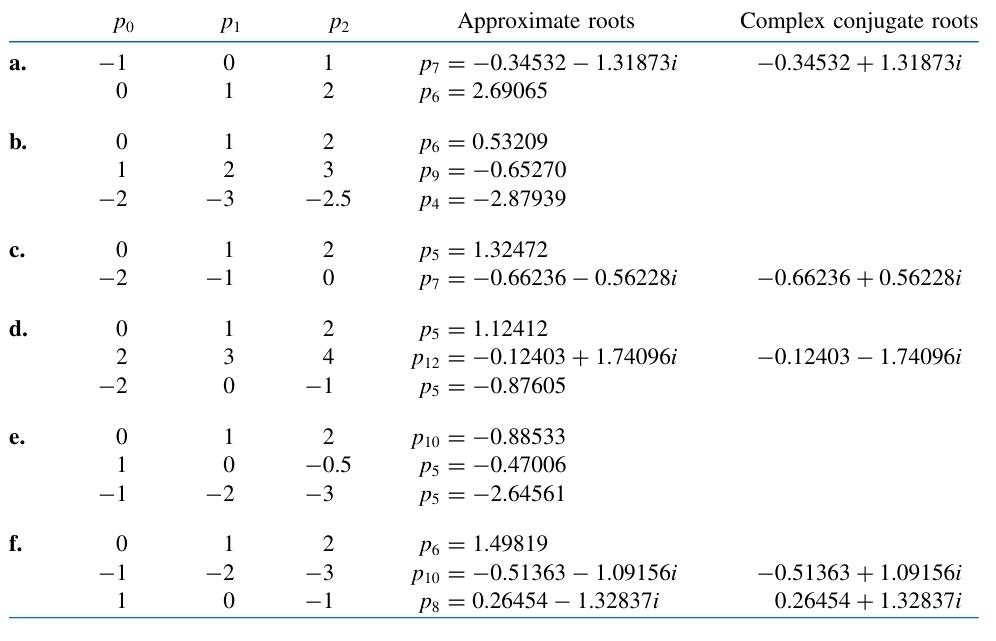
\includegraphics[width=15cm]{EndofMod2Q3sol}
\end{center}
\item 
\begin{enumerate}[label=(\alph*)]
\item $\left|\frac{f''(\xi)}{2} (0.45-0)(0.45-0.6)\right|\leq0.135$; $\left|\frac{f'''(\xi)}{6}(0.45-0)(0.45-0.6)(0.45-0.9)\right|\leq0.00397$\\
\item $\left|\frac{f''(\xi)}{2} (0.45-0)(0.45-0.6)\right|\leq0.03375$; $\left|\frac{f'''(\xi)}{6}(0.45-0)(0.45-0.6)(0.45-0.9)\right|\leq0.001898$\\
\item $\left|\frac{f''(\xi)}{2} (0.45-0)(0.45-0.6)\right|\leq0.135$; $\left|\frac{f'''(\xi)}{6}(0.45-0)(0.45-0.6)(0.45-0.9)\right|\leq0.010125$\\
\item $\left|\frac{f''(\xi)}{2} (0.45-0)(0.45-0.6)\right|\leq0.06779$; $\left|\frac{f'''(\xi)}{6}(0.45-0)(0.45-0.6)(0.45-0.9)\right|\leq0.151$
\end{enumerate}
\end{enumerate}
\end{mysolution}
\end{posttest}

%share your understanding of properties of functions and their applications to solving rates of change problems in physical phenomenon 


%\end{actsoln}

\takehome

\comy{You are now at the last part of this module. Your  task is to do a self-reflection on your learning experience. In ypur own words describe what you have learnt in this module.}



\references
\begin{refenumerate}
\item Kong, Q., Siauw, T., Bayen, A., (2020). Python Programming and Numerical Methods. First Edition, Academic Press,  ISBN-13 ‏ : ‎ 978-0128195499 \\
\mylink{https://pythonnumericalmethods.studentorg.berkeley.edu/notebooks/Index.html}
%chapter 1 pg 7-36 functions\\
%chapter 1 pg 51-83 limits and continuity\\
%chapter 1 pg 45-50 rates of change\\
%chapter 2 pg 108-120 the derivative\\
%\item Mendelson, E. (2022). Schaum's Outline of Calculus. McGraw-Hill Education.
%chapter 6 51-55 functions
%chapter 7 59-65 limits
%chapter 8 69-74 continuity
%chapter 9 77-81 derivative
%\item Calculus \mylink{https://math.libretexts.org/Bookshelves/Calculus}
%\item Chris McMullen, 2021, Essential Calculus Skills Practice Workbook with Full Solutions, Zishka Publishing, ISBN 978-1-941691-24-3
%\item R. Adams and C. Essex, 2021, Calculus: A complete Course, Addison Wesley, ISBN 13: 978-0135732588
%\item P. Abbott and H. Neill, 2018, Calculus: A Complete Introduction: The Easy Way to Learn Calculus (Teach Yourself), ISBN 13: 978-1473678446
\end{refenumerate}





%\wrapup
%To wrap-up, answer the following questions:
%
%\begin{enumerate}
%\item 
%%when do we say that a limit of a function exists?
%%\item how do we remove discontinuity in functions?
%%\item what is the relationship between the gradient of the tangent line and the derivative?
%\end{enumerate}
















%\newpage

%\facilitation


%
\begin{center}
    {\Large \textbf{FUNCTIONS OF SEVERAL VARIABLES}}\\[2mm]
(DEFINITION, DOMAIN, RANGE, GRAPHS AND LEVEL CURVES) \\[4mm]

\mycenterbox{5 minute review}%\\[4mm]
Recap the definition of a function of several variables, and the meaning of domain, range, graph and level curves of functions of several variables.
\end{center}
\mycenterbox{Warm-up.}%\\[4mm]
\problemAnswer{
Match the function with its graph (labeled I–VI).Give reasons for your choices
\begin{multicols}{3}
\begin{enumerate}[label=(\alph*)]
\item $f(x,y)=|x|+|y|$\\[4mm]
\item $f(x,y)=|xy|$
\item $f(x,y)=\frac{1}{1+x^2+y^2}$\\2mm]
\item $f(x,y)=(x^2-y^2)^2$
\item $f(x,y)=(x-y)^2$\\[4mm]
\item $f(x,y)=\sin(|x|+|y|)$
\end{enumerate}
\end{multicols}

\begin{center}
%\centering
\includegraphics[width=10cm]{MCTutorial1Q1.JPEG}
\end{center}
%\tcbox[tcbox raise base]{Warm-up}
 
%\begin{flushright}
%\begin{tikzpicture}
%    % A body
%
%
%    % Non-rectangle shapes must be drawn as polygone
%    \begin{scope}[shift={(3,0)}]
%        \draw  (0,0.5) -- (0,4) -- (.5,4) -- (.5,4.5) -- (1.,4.5) -- (4.,4.5) --(4.,4)-- (4.5,4) --(4.5,0.5) --(4.0,0.5)--(4.0,0.0)-- (.5,0) --(0.5,0.5) -- cycle;
%        % Draw symmetry lines
%        \draw [symmetry] (.5, 0.5) -- (.5,4.0);
%        \draw [symmetry] (4, 0.5) -- (4,4.0);
%        \draw [symmetry] (.5,4.0) -- (4,4.0);
%         \draw [symmetry] (.5, 0.5) -- (4, 0.5);
%        % Dimensions
%        \draw (4.5,0) -- ++(0.5,0) coordinate (D1) -- +(5pt,0);
%        \draw (4.5,4.5) -- ++(0.5,0) coordinate (D2) -- +(5pt,0);
%        \draw [dimen] (D1) -- (D2) node {6cm};
%       
%        
%        \draw (0.0,5) -- ++(0,0.5) coordinate (D1) -- +(0,+5pt);
%        \draw (0.5,5) -- ++(0,0.5) coordinate (D2) -- +(0,+5pt);
%        \draw [dimen,-] (D1) -- (D2) node [above=5pt] {$x$ cm};
%        \draw [dimen,<-] (D1) -- ++(-5pt,0);
%        \draw [dimen,<-] (D2) -- ++(+5pt,0);
%    \end{scope}
%\end{tikzpicture}
%\end{flushright}

}


\mycenterbox{Problems.}%

%\begin{center}
%\tcbox[tcbox raise base]{ Problems. Choose from the below}
%\end{center}
\problem{Exploring functions}%
\begin{enumerate}[(a)]
\item Are the following functions even, odd, or neither? What can you say
about their range?
\begin{multicols}{4}
 \begin{enumerate}[(i)]
\item $\displaystyle \frac{3x}{x^2+2}$
\item $\displaystyle \cos x+3$
\item $\displaystyle \frac{2x^3}{\cos x+3}$
\item $\displaystyle \frac{3x^4+2x^2}{\sin x+4}$
\end{enumerate}
\end{multicols}
\item Consider the functions $\sin^n x$ and $\cos^n x$, where $n$ is a positive integer.
Which are odd, which are even, and what are their periodicities?
\item What is the periodicity of $f(x) = 2 \cos x+\sin 2x$? Is it even/odd/neither?

\end{enumerate}

\problem{Cubic functions} 
Show that $x-1$ is a factor of the cubic function%
$$P(x)=x^3-2x^2-5x+6,$$
and  find the quadratic factor $Q(x)$ such that $P(x) = (x -1)Q(x)$. Factorise
$Q(x)$ and hence sketch $P(x).$

%\newpage
\problem{Sigmoid functions*.}%
For positive integers $n$, consider the family of functions
$$\displaystyle f_n= \frac{x^n}{2^n+x^n}.$$
\begin{enumerate}[(a)]
\item What are appropriate domains and ranges for $f_n(x)$? Do they depend on $n$?

\item Is $f_n(x)$ even, odd, or neither? Does this depend on $n$?

\item Show that for $x\geq 0$, $f_n(x)$ are strictly increasing functions and that
$0\leq f_n(x) < 1.$
\item What is the value of $f_n(2)$? Does it depend on $n$?

\item By considering the values of $f_n(1.9)$ and $f_n(2.1)$ for $n = 2, 4, 8, 16, 32$ and
$64$, show that the graph of $f_n(x)$ for $x\ge 0$ is an increasing sigmoid (that
is, $S$-shaped) function that approaches a step function as $n\rightarrow \infty$.
\end{enumerate}

\mycenterbox{Selected answers and hints}%

For the warm-up, $V(x)=4x(3-x)^2$. Writing $x=1+\epsilon$, we get
$$V = 4(1 +\epsilon)(3- (1+\epsilon))^2=4(4-\epsilon^2(3-\epsilon)).$$
If $-1<\epsilon<2$ then $\epsilon^2 (3-\epsilon)\ge 0$, with equality when $\epsilon=0$. Thus the maximum
value of $V$ occurs when $\epsilon= 0$, i.e. $x = 1\rm{cm}$.

\begin{enumerate}
\item 
\begin{enumerate}[(i)]
\item Odd. The range is the interval  $[-\frac{3}{4}\sqrt{2},\; \frac{3}{4}\sqrt{2}]$
\item Even. The range is the interval $[2, 4]$.
\item Odd. The range is all of $\mathbb R$.
\item Neither. (For example, writing $\displaystyle \frac{5}{\sin x+4}$ we have $\displaystyle f(1)= \frac{5}{\sin (1)+4} \equiv 1.032 (3\rm{dp})$ which is neither $f(1)$ nor $-f(1)$.)\\[4mm]
The range is the nonnegative reals $[0,\infty)$

\end{enumerate}
\end{enumerate}











%
%\newpage
%
%\newpage
%
%
%\newtheorem{definition}[subsection]{Definition}
%\newtheorem{example}[subsection]{Example}
%\newtheorem{cor}[subsection]{Corollary}
\newtheorem{pro}[subsection]{Proposition}
\newtheorem{theo}[subsection]{Theorem}
\newtheorem{lem}[subsection]{Lemma}
%\newtheorem{rem}[subsection]{Remark}

\definecolor{main}{HTML}{5989cf}    % setting main color to be used
\definecolor{sub}{HTML}{cde4ff}     % setting sub color to be used

\tcbset{
    sharp corners,
    colback = white,
    before skip = 0.2cm,    % add extra space before the box
    after skip = 0.5cm      % add extra space after the box
}                           % setting global options for tcolorbox

% You can copy any following box you like to your code.
\newtcolorbox{boxA}{
    fontupper = \bf,
    boxrule = 1.5pt,
    colframe = black % frame color
}

\newtcolorbox{boxB}{
    fontupper = \bf\color{main}, % font color
    boxrule = 1.5pt,
    colframe = main,
    rounded corners,
    arc = 5pt   % corners roundness
}
\newtcolorbox{boxC}{
    colback = sub, % background color
    boxrule = 0pt  % no borders
}

\newtcolorbox{boxD}{
    colback = sub, 
    colframe = main, 
    boxrule = 0pt, 
    toprule = 3pt, % top rule weight
    bottomrule = 3pt % bottom rule weight
}

\hypersetup{
    colorlinks=true,
    linkcolor=blue,
    filecolor=magenta,      
    urlcolor=cyan,
    pdftitle={Overleaf Example},
    pdfpagemode=FullScreen,
    }

\urlstyle{same}


\coursetitle{\mtthreeiii}{MT303}
\developers{Wyclife Rao}
\reviewers{Dr Irene Sitawa}
\modulenumber{3}
\modulename{Interpolation and Polynomial Approximation}

% courses
\thispagestyle{empty}
\begin{tikzpicture}[overlay,remember picture,font=\sffamily\bfseries]
 \draw[ultra thick,c4,name path=big arc] ([xshift=-2mm]current page.north) arc(150:285:11) coordinate[pos=0.225] (x0);
 \begin{scope}
  \clip ([xshift=-2mm]current page.north) arc(150:285:11) --(current page.north east);
  \fill[c4!50,opacity=0.25] ([xshift=4.55cm]x0) circle (4.55);
  \fill[c4!50,opacity=0.25] ([xshift=3.4cm]x0) circle (3.4);
  \fill[c4!50,opacity=0.25] ([xshift=2.25cm]x0) circle (2.25);
  \draw[ultra thick,c4!50] (x0) arc(-90:30:6.5);
  \draw[ultra thick,c4] (x0) arc(90:-30:8.75);
  \draw[ultra thick,c4!50,name path=arc1] (x0) arc(90:-90:4.675);
  \draw[ultra thick,c4!50] (x0) arc(90:-90:2.875);
  \path[name intersections={of=big arc and arc1,by=x1}];
  \draw[ultra thick,c4,name path=arc2] (x1) arc(135:-20:4.75);
  \draw[ultra thick,c4!50] (x1) arc(135:-20:8.75);
  \path[name intersections={of=big arc and arc2,by={aux,x2}}];
  \draw[ultra thick,c4!50] (x2) arc(180:50:2.25);
 \end{scope} 
 \path[decoration={text along path,text color=c4,
                 raise = -2.8ex,
                 text  along path,
                 text = {},%|\sffamily\bfseries|02/18/2019
                 text align = center,
             },
             decorate
         ] ([xshift=-2mm]current page.north) arc(150:245:11);
 %
 \newcommand\add{4cm}
 \begin{scope}%[shift={(5,0)}]
  \path[clip,postaction={fill=c3}]
  ([xshift=2cm+\add,yshift=-8cm]current page.center) rectangle ++ (4.6,7.7);
  \draw[c5,ultra thick,fill=c2] ([xshift=0.5cm+\add,yshift=-8cm]current page.center)
   ([xshift=0.5cm+\add,yshift=-8cm]current page.center)  arc(180:60:2)
    |- ++ (-3,6) --cycle;
  \draw[ultra thick,c5] ([xshift=-1.5cm+\add,yshift=-8cm]current page.center) 
  arc(180:0:2);
  \draw[ultra thick,c5] ([xshift=0.5cm+\add,yshift=-8cm]current page.center) 
  arc(180:0:2);
  \draw[ultra thick,c5] ([xshift=2.5cm+\add,yshift=-8cm]current page.center) 
  arc(180:0:2);
  \draw[ultra thick,c5] ([xshift=4.5cm+\add,yshift=-8cm]current page.center) 
  arc(180:0:2);
  \fill[white] ([xshift=2.5cm+\add,yshift=-8cm]current page.center) +(60:2) circle(1.5mm)
  node[above
  right=0mm,text=c5!80!black]{$\rho:=\dfrac{1+\sqrt{-3}}{2}$};
 \end{scope}
 %
 \fill[c1] ([xshift=2cm+\add,yshift=-8cm]current page.center) rectangle ++ (-30.7,7.7);
 \node[text=white,anchor=west,scale=2.3,inner sep=0pt] at
 ([xshift=-10cm,yshift=-1.8cm]current page.center) {\color{ulabgold} LEARNING};
 \node[text=white,anchor=west,scale=5,inner sep=0pt] at
 ([xshift=-10cm,yshift=-3.25cm]current page.center) {MODULE \dpmdnumber};
 \node[text=white,anchor=west,scale=2.5,inner sep=0pt,text width=.4\textwidth] at
 ([xshift=-10cm,yshift=-6cm]current page.center) {\dpmdname};
 \node[text=white,anchor=east,scale=2,inner sep=0pt] at
 ([xshift=5.7cm,yshift=-7.5cm]current page.center) {\color{ulabgold}The Open University of Kenya};
 %
% \draw[gray,line width=5mm] 
% ([xshift=2mm,yshift=-1mm]current page.south west) rectangle ([xshift=-2mm,yshift=1mm]current
% page.north east);
\end{tikzpicture}

%\newpage
\pagenumbering{roman}
\thispagestyle{empty}%firstpage


\begin{center}
\vspace*{2cm}
{\Huge\bf BACHELOR OF TECHNOLOGY EDUCATION}\\[3cm]  


%{\fontsize{80}{40}\selectfont \dpcoursecode}\\[2cm]
%
%{\fontsize{30}{40} \selectfont \dpcoursename}\\[2cm]

%\rule{\textwidth}{1pt}
%\vspace{2cm}

%{\fontsize{40}{40}\selectfont \bf Module~\dpmdnumber}\\[2cm]
%
%{\fontsize{30}{40}\selectfont \bf \dpmdname}\\

\vfill
\begin{flushright}
\begin{minipage}{.6\textwidth}
\begin{tcolorbox}%[text ]
\begin{tabular}{ll}%\hline
\subtitle{Developed by:}&\displaydevelopers\\
&\\
\subtitle{Reviewed by:}&\makecell[l]{\displayreviewers}\\
\end{tabular}
\end{tcolorbox}
\end{minipage}\hspace*{-3.5cm}
\end{flushright}
\vspace*{-2.5cm}
\end{center}

\newpage
\thispagestyle{empty}
\null
\vfill
{\renewcommand\arraystretch{1.5}
\begin{tabular}{|l|l|}\hline
\subtitle{Programme Title} & Bachelor of Technology Education \\\hline
\subtitle{Course Title} & \fullcoursename\\\hline
\subtitle{Learning Module number} & Module \dpmdnumber\\\hline
\subtitle{Learning module title} & \dpmdname \\\hline
\subtitle{Module Developer} & \displaydevelopers\\\hline
\subtitle{Reviewed by} & \displayreviewers\\\hline
%\subtitle{Vision} & \vision\\\hline
%\subtitle{Audience description} & \\\hline
\end{tabular}}
\clearpage

%\section{COURSE LEARNING GUIDE}


\subsection*{Preparing for Online and Distance Learning}

This course offers you the opportunity to enter an online space where you can engage with fellow students at the university. The online forums, exercises, tasks and materials have been designed by the course facilitators in such a way that you can draw directly from their knowledge and share in their scholarly interest in online learning and assessment

We hope you will use your access to this virtual classroom to raise all your questions on the course module, to build a network great learners and to share your own thoughts and experiences to the benefit of your fellow students.

   
There are a number of steps you can take to ensure you are well prepared to make the most of this learning opportunity. This resource should prompt you to consider the following:


 \begin{enumerate}[label=\cb$\square$]
   \item How can you best prepare the space where you expect you will spend most of your time engaging in online learning (i.e. in your home or office, or even during your commute to work or whilst traveling)?
  \item   What can you do to ensure you keep working through the course material, even when you do not have Internet access?
    \item How can you familiarise yourself with the course layout, in order to be able to navigate through the steps with ease?
    \item What are the communication strategies and best practices you could consider to best engage with your fellow students and the course facilitators?
    \item What do you do when you need academic or technical support?

 \end{enumerate} 

\subsection*{General Module Guide}

The authors of this module believe that imparting knowledge should always be a mutual relationship between the students and the teachers. Students can actively construct knowledge through experiences gained in reading and answering the learning modules.

You should take time to read everything written in the module, actively and religiously solve all the exercises included to finish this course and be able to gain all the competencies and skills expected to demonstrate the learning outcomes as stated in this course. If you finish with full confidence that you understand and can apply all the knowledge you gain in this course, then you are sure to succeed in tackling the next higher subjects in your chosen course.

In this course, you will be taught not only the knowledge you need to demonstrate your learning outcomes, but you will also gain discipline, perseverance, higher thinking skills, and resourcefulness that would help strengthen your foundation to succeed in life. To successfully finish the course, you must follow the guides set forth in using this module.


\begin{description}[{format=\textcolor{ulabblue}}]
\item[STUDY ENVIRONMENT.]\leavevmode\\
Before engaging into the module, make sure that you are comfortable enough and diminish distractions. Make sure that you develop a study routine to perform and accomplish all the activities set forth by the module.
%\newpage

\item[MODE OF DELIVERY.]\leavevmode\\
Students are required to get a access a digitised copy of the module from the Virtue Learning Environment. As an open and distance learner, you should be able to learn independently and optimise the learning modes and environment available to you as much of  the delivery of all the lessons will be done asynchronously. Your success will greatly depend on your self-motivation and discipline to get your work done without your instructor to remind you from time to time.

\item[STUDY SCHEDULE.] \leavevmode\\
Remember that you have other subjects to attend to, hence, you must manage your time so that you will not be left behind in any of them. Create your own learning plan for each course to make sure that you can perform all the activities. Do not procrastinate your work, remember that time wasted can never be retrieved back. Make sure that even if you are at home, you are a student enrolled in a program, where the learning of all its courses greatly depends on your will to learn as the materials you need are all in your hands. So always be aware of your daily tasks.

\item[PRACTICE EXERCISE.]\leavevmode\\
To measure your learning from your reading, you are given practice exercises which you are supposed to answer daily. This will prepare you in performing your main task.

\item[ONLINE GROUP CHAT.]\leavevmode\\
I am going to create an online Discussion Forum and QA Forum  on the VLE.  This will serve as a room for discussion on the topics and activities found in your module.

\item[RECOMMENDED REFERENCES FOR SUPPLEMENTARY READING.]\leavevmode\\
You are given links that you need to access online. These links are online references such as e-books, online activities, and tutorial videos of the topic. These are other references you can use to further understand the topic and gain additional knowledge and skills.

\item[MAIN TASK.]\leavevmode\\
You are given a task that will require you to apply the knowledge and skills you learned from the module. This can be a group or individual activity which will measure your higher order thinking skills you acquired throughout the topic.

\item[RUBRICS. ]\leavevmode\\
This is a tool to guide you in performing your main task. Through this, you will be able to know the specific indicators that should be found in your task. This is to assess your constructive behaviour towards your learning application. You will be rated according to a 4-point scale shown below.
\begin{center}
{\color{ulabgold} \bf 4 − Excellent\quad\quad   3 −Good\quad\quad    2 − Fair \quad\quad  1 −Poor}
\end{center}
\item[REFLECTIONS.]\leavevmode\\
Writing your reflection will be a passageway to express your experiential learning in using this module. In your honest recall, write everything that you think happened to you during your learning experience in this module. Use the guide questions below:
\begin{description}[{format=\textcolor{ulabblue}}]
\item[First paragraph. ]\leavevmode\\
How was your learning experience? Maybe you can consider describing the effect of the parts of the module (sequence, discussions, examples, practice exercises, online activities, and the main task) in your learning experience. You can point out the strength and weakness of each part so that we can consider it for future improvement of this instructional material.
\item[Second paragraph.  ]\leavevmode\\
What did you learn? Did you successfully acquire the learning outcomes?

\item[Third paragraph.]\leavevmode\\
How can you use what you learned in the future?
\end{description}
\end{description}

\section{ASSESSMENT  TASKS \& EXAMINATION   RULES AND GUIDELINES}

\begin{enumerate}[label=\cb\arabic*.]
\item {\cb SUBMISSION OF ASSESSMENT TASTS.}

Since mathematical skills are best acquired through constant practice, you are encouraged to answer at least two (2) exercises a day. These practice exercises will not be graded but it will help you develop your thinking skills which will prepare you in the performance of your main tasks. You are required to submit your practice exercises every week.
\begin{center} {\cg Usually submission deadlines are set on Saturday 11:59PM EAT} \end{center}

\item  {\cb GROUP CHAT.}

You can post questions, solutions, and comment to other's post. Please be reminded that our group chat is exclusive only for discussion on topics related to this course. Everyone is required to actively participate in the discussions. Also, trolling is highly discouraged. Always observe proper online etiquettes when participating in discussions.
\begin{center} {\cb RULE OF THUMB: ALWAYS THINK BEFORE YOU CLICK} \end{center}

\item  {\cb MAIN TASK. }

Complete documentation during the preparation of your task is required to ensure that every member of the group participated and contributed in the task. May it be photos or screenshots of your virtual meetings or group works. You are going to submit it as attachment of your main task the same way as the practice exercises.



\item {\cb RECOMMENDED REFERENCES FOR SUPPLEMENTARY READING.} 

You can explore online for other references that is related to the topic to gain additional information about the topic. Do not share or post inappropriate materials online or even privately.
\end{enumerate}

\subsection*{Requirements to pass the course}

Compiled Continuous  Assignment/Activities and Tasks  with Final Performance Examination.

\subtitle{Grading System}
\begin{center}
{\renewcommand\arraystretch{1.5}
\begin{tabular}{|l|c|}\hline
Continuous Activities and Tasks  &  50\%\\\hline
Final Performance Examination. &  50\%\\\hline
\end{tabular}
}
\end{center}
%\newpage










%\subsection{INTRODUCTORY MESSAGE}

%A warm welcome to \;  \fullcoursename, {\bf Module on \dpmdname}.



%By this module learning resource, we aim to enable you  achieve the relevant competencies, depict skill, action and purpose successfully. 
 

%It has been designed to provide you with fun and meaningful opportunities for guided and independent learning at your own pace and time. You will be enabled to process the contents of the learning material while being an active learner. Your academic success lies in your own hands.  This module has the following parts and corresponding icons:





{
\renewcommand\arraystretch{4}
\begin{longtblr}{
width=\linewidth,
 colspec={ Q[1,c,f] Q[1.5,r,m] Q[4,l,m] },
%row{1} = { font=\bfseries },
% rowhead = 1,
  caption={ }, 
  label={ },
  rowsep = 4pt,
  hlines = {ulabblue!20, 1pt},
  vlines = {ulabblue!20, 1pt},
}

\includegraphics[width=2cm]{img/audience} & {\bf AUDIENCE}  &  This is a description of a target audience.   \\
{\fontsize{40}{30}\selectfont\color{ulabblue}\faCogs}& {\bf MODULE DESCRIPTION} & 
This part explains the importance of the topics discussed in the module. It will also give you a sneak peek of what you will learn and what is expected from you at the end of the module.\\

\includegraphics[width=2cm]{img/target.png} &  {\bf  EXPECTATION} & These are what you will be able to know after completing the lessons in the module\\

\includegraphics[width=2cm]{img/preactivities} & {\bf PRE-ACTIVITY} &
This activity is to get you set, activate and engage schema to learn the module. Through this activity, you will know the relevance of this activity to the topic that will be discussed in the module.\\

\includegraphics[width=2cm]{img/pretest} &  {\bf PRE - ASSESSMENT} & This will measure your prior knowledge and the concepts to be mastered throughout the lesson. \\

\includegraphics[width=1.7cm]{img/rewind} &  {\bf  RECAP} & This section will measure what learnings and skills that you understand from the previous lesson.\\

\includegraphics[width=1.5cm]{img/lesson} &  {\bf  LESSON} & This section will discuss the topic for this module.\\

\includegraphics[width=2cm]{img/activities} &  {\bf  ACTIVITIES} & This is a set of activities you will perform.\\

\includegraphics[width=2cm]{img/summary} &  {\bf  WRAP UP} & This section summarizes the concepts and applications of the lessons.\\

\includegraphics[width=2cm]{img/discussion}& {\bf DISCUSSIONS} &
This is the meat of the module. The discussion is aligned to the topic learning outcomes that is expected of you to acquire at the end of the module.\\

\includegraphics[width=1.8cm]{img/value} &  {\bf  VALUING} & This part will check the integration of values in the learning competency you will take home.\\

\includegraphics[width=1.8cm]{img/posttest} &  {\bf  POST - ASSESSMENT} & This will measure how much you have learned from the entire module.\\

\includegraphics[width=1.8cm]{img/selfreflect} & {\bf REFLECTION }
&
This part is for you to share your thoughts by writing your reflection, make sure to check your grammar and spelling to ensure the readability and so that it will not alter the thought being delivered. 
\end{longtblr}
}









%\vfill

\audience
\begin{oldactivity}{Audience Description}{
\includegraphics[width=22mm]{img/audience}}{}
This module is offered to all students taking the Bachelor of Technology Education. As an open and distance learner, you should be able to learn independently and optimise the learning modes and environment available to you. Before you begin this course, please confirm the course material, the course requirements and how the course is conducted.
\end{oldactivity}
%\newpage
\pagenumbering{arabic}



\mddescription
This module guides you into a detailed discussion of the concepts of interpolation and polynomial approximation. Specifically you will learn about
\begin{itemize}
\item data approximation and Nevill's method
\item divided differences
\item Hermite interpolation
\item cubuc spline interpolation 
\end{itemize}
%\expectations
%\begin{objenumerate}
%
%\end{objenumerate}

\begin{mlos}
\item Identify the steps involved in Neville’s algorithm and divided differences.
\item Describe the principles of Hermite interpolation and cubic splines.
\item Construct interpolating polynomials and cubic splines for given data sets.
\item Develop smooth curve approximations using cubic spline interpolation for real-world data. 
\end{mlos}

\section{Data Approximation and Neville's Method}
\videolesson
\begin{selfvideo}[1]
%LESSON 3: 
This video presents a discussion on data approximation and Nevill's method. Follow the discussion and then solve the problems in the subsequent quiz.
\end{selfvideo}
%\begin{boxB}Question: \end{boxB}
In Section $4$ of Module $2$ we found an explicit representation for Lagrange polynomials and their error when approximating a function on an interval. A frequent use of these polynomials involves the interpolation of tabulated data. In this case an explicit representation of the polynomial might not be needed, only the values of the polynomial at specified points. In this situation the function underlying the data might not be known so the explicit form of the error cannot be used. We will now illustrate a practical application of interpolation in such a situation.

\begin{example}
Table \ref{table:dataexample1} lists values of a function $f$ at various points. The approximations to $f(1.5)$ obtained by various Lagrange polynomials that use this data will be compared to try and determine the accuracy of the approximation. The most appropriate linear polynomial uses $x_{0}=1.3$ and $x_{1}=1.6$ because $1.5$ is between $1.3$ and $1.6$. The value of the interpolating polynomial at $1.5$ is
\[\begin{aligned}
P_{1}(1.5) & =\frac{(1.5-1.6)}{(1.3-1.6)} f(1.3)+\frac{(1.5-1.3)}{(1.6-1.3)} f(1.6) \\
& =\frac{(1.5-1.6)}{(1.3-1.6)}(0.6200860)+\frac{(1.5-1.3)}{(1.6-1.3)}(0.4554022)=0.5102968
\end{aligned}\]
Two polynomials of degree $2$ can reasonably be used, one with $x_{0}=1.3, x_{1}=1.6$, and $x_{2}=1.9$, which gives
\[\begin{aligned}
P_{2}(1.5)= & \frac{(1.5-1.6)(1.5-1.9)}{(1.3-1.6)(1.3-1.9)}(0.6200860)+\frac{(1.5-1.3)(1.5-1.9)}{(1.6-1.3)(1.6-1.9)}(0.4554022) \\
& +\frac{(1.5-1.3)(1.5-1.6)}{(1.9-1.3)(1.9-1.6)}(0.2818186)=0.5112857
\end{aligned}\]
and one with $x_{0}=1.0, x_{1}=1.3$, and $x_{2}=1.6$, which gives $\hat{P}_{2}(1.5)=0.5124715$.

In the third-degree case, there are also two reasonable choices for the polynomial. One with $x_{0}=1.3, x_{1}=1.6, x_{2}=1.9$, and $x_{3}=2.2$, which gives $P_{3}(1.5)=0.5118302$.

The second third-degree approximation is obtained with $x_{0}=1.0, x_{1}=1.3, x_{2}=1.6$, and $x_{3}=1.9$, which gives $\hat{P}_{3}(1.5)=0.5118127$. The fourth-degree Lagrange polynomial uses all the entries in the table. With $x_{0}=1.0, x_{1}=1.3, x_{2}=1.6, x_{3}=1.9$, and $x_{4}=2.2$, the approximation is $P_{4}(1.5)=0.5118200$.

Because $P_{3}(1.5), \hat{P}_{3}(1.5)$, and $P_{4}(1.5)$ all agree to within $2 \times 10^{-5}$ units, we expect this degree of accuracy for these approximations. We also expect $P_{4}(1.5)$ to be the most accurate approximation, since it uses more of the given data.

The function we are approximating is actually the Bessel function of the first kind of order zero, whose value at $1.5$ is known to be $0.5118277$. Therefore, the true accuracies of the approximations are as follows:
\[\begin{aligned}
\left|P_{1}(1.5)-f(1.5)\right| & \approx 1.53 \times 10^{-3}, \\
\left|P_{2}(1.5)-f(1.5)\right| & \approx 5.42 \times 10^{-4}, \\
\left|\hat{P}_{2}(1.5)-f(1.5)\right| & \approx 6.44 \times 10^{-4}, \\
\left|P_{3}(1.5)-f(1.5)\right| & \approx 2.5 \times 10^{-6}, \\
\left|\hat{P}_{3}(1.5)-f(1.5)\right| & \approx 1.50 \times 10^{-5}, \\
\left|P_{4}(1.5)-f(1.5)\right| & \approx 7.7 \times 10^{-6} .
\end{aligned}\]
Although $P_{3}(1.5)$ is the most accurate approximation, if we had no knowledge of the actual value of $f(1.5)$, we would accept $P_{4}(1.5)$ as the best approximation since it includes the most data about the function.
% The Lagrange error term derived in Theorem $7$ of Module $2$ cannot be applied here because we have no knowledge of the fourth derivative of $f$. Unfortunately, this is generally the case.
\end{example}

\begin{table}
\centering
\begin{tabular}{cc}
\hline
$x$ & $f(x)$ \\
\hline
1.0 & 0.7651977 \\
1.3 & 0.6200860 \\
1.6 & 0.4554022 \\
1.9 & 0.2818186 \\
2.2 & 0.1103623 \\
\hline
\end{tabular}
\caption{\scriptsize Table 1 Example 1}
\label{table:dataexample1}
\end{table}

\subsection*{Neville's Method}
A practical difficulty with Lagrange interpolation is that the error term is difficult to apply, so the degree of the polynomial needed for the desired accuracy is generally not known until computations have been performed. A common practice is to compute the results given from various polynomials until appropriate agreement is obtained, as was done in the previous Illustration. However, the work done in calculating the approximation by the second polynomial does not lessen the work needed to calculate the third approximation; nor is the fourth approximation easier to obtain once the third approximation is known, and so on. We will now derive these approximating polynomials in a manner that uses the previous calculations to greater advantage.

\begin{definition}
Let $f$ be a function defined at $x_{0}, x_{1}, x_{2}, \ldots, x_{n}$, and suppose that $m_{1}, m_{2}, \ldots, m_{k}$ are $k$ distinct integers, with $0 \leq m_{i} \leq n$ for each $i$. The Lagrange polynomial that agrees with $f(x)$ at the $k$ points $x_{m_{1}}, x_{m_{2}}, \ldots, x_{m_{k}}$ is denoted $P_{m_{1}, m_{2}, \ldots, m_{k}}(x)$.
\end{definition}

\begin{example}\label{example:numb2}
Suppose that $x_{0}=1, x_{1}=2, x_{2}=3, x_{3}=4, x_{4}=6$, and $f(x)=e^{x}$. Determine the interpolating polynomial denoted $P_{1,2,4}(x)$, and use this polynomial to approximate $f(5)$.
\end{example}

\begin{mysolution}
This is the Lagrange polynomial that agrees with $f(x)$ at $x_{1}=2, x_{2}=3$, and $x_{4}=6$. Hence
\[P_{1,2,4}(x)=\frac{(x-3)(x-6)}{(2-3)(2-6)} e^{2}+\frac{(x-2)(x-6)}{(3-2)(3-6)} e^{3}+\frac{(x-2)(x-3)}{(6-2)(6-3)} e^{6}.\]
So
\[\begin{aligned}
f(5) \approx P(5) & =\frac{(5-3)(5-6)}{(2-3)(2-6)} e^{2}+\frac{(5-2)(5-6)}{(3-2)(3-6)} e^{3}+\frac{(5-2)(5-3)}{(6-2)(6-3)} e^{6} \\
& =-\frac{1}{2} e^{2}+e^{3}+\frac{1}{2} e^{6} \approx 218.105
\end{aligned}\]
\end{mysolution}

The next result describes a method for recursively generating Lagrange polynomial approximations.

\begin{theorem}\label{thm:data1}
Let $f$ be defined at $x_{0}, x_{1}, \ldots, x_{k}$, and let $x_{j}$ and $x_{i}$ be two distinct numbers in this set. Then
\[P(x)=\frac{\left(x-x_{j}\right) P_{0,1, \ldots, j-1, j+1, \ldots, k}(x)-\left(x-x_{i}\right) P_{0,1, \ldots, i-1, i+1, \ldots, k}(x)}{\left(x_{i}-x_{j}\right)}\]
is the $k$ th Lagrange polynomial that interpolates $f$ at the $k+1$ points $x_{0}, x_{1}, \ldots, x_{k}$.
\end{theorem}
%Proof For ease of notation, let $Q \equiv P_{0,1, \ldots, i-1, i+1, \ldots, k}$ and $\hat{Q} \equiv P_{0,1, \ldots, j-1, j+1, \ldots, k}$. Since $Q(x)$ and $\hat{Q}(x)$ are polynomials of degree $k-1$ or less, $P(x)$ is of degree at most $k$.
%
%First note that $\hat{Q}\left(x_{i}\right)=f\left(x_{i}\right)$, implies that
%
%$$
%P\left(x_{i}\right)=\frac{\left(x_{i}-x_{j}\right) \hat{Q}\left(x_{i}\right)-\left(x_{i}-x_{i}\right) Q\left(x_{i}\right)}{x_{i}-x_{j}}=\frac{\left(x_{i}-x_{j}\right)}{\left(x_{i}-x_{j}\right)} f\left(x_{i}\right)=f\left(x_{i}\right)
%$$
%
%Similarly, since $Q\left(x_{j}\right)=f\left(x_{j}\right)$, we have $P\left(x_{j}\right)=f\left(x_{j}\right)$.\\
%In addition, if $0 \leq r \leq k$ and $r$ is neither $i$ nor $j$, then $Q\left(x_{r}\right)=\hat{Q}\left(x_{r}\right)=f\left(x_{r}\right)$. So
%
%$$
%P\left(x_{r}\right)=\frac{\left(x_{r}-x_{j}\right) \hat{Q}\left(x_{r}\right)-\left(x_{r}-x_{i}\right) Q\left(x_{r}\right)}{x_{i}-x_{j}}=\frac{\left(x_{i}-x_{j}\right)}{\left(x_{i}-x_{j}\right)} f\left(x_{r}\right)=f\left(x_{r}\right) .
%$$
%
%But, by definition, $P_{0,1, \ldots, k}(x)$ is the unique polynomial of degree at most $k$ that agrees with $f$ at $x_{0}, x_{1}, \ldots, x_{k}$. Thus, $P \equiv P_{0,1, \ldots, k}$.

Theorem \ref{thm:data1} implies that the interpolating polynomials can be generated recursively. For example, we have
\[\begin{aligned}
P_{0,1} & =\frac{1}{x_{1}-x_{0}}\left[\left(x-x_{0}\right) P_{1}-\left(x-x_{1}\right) P_{0}\right], \quad P_{1,2}=\frac{1}{x_{2}-x_{1}}\left[\left(x-x_{1}\right) P_{2}-\left(x-x_{2}\right) P_{1}\right], \\
P_{0,1,2} & =\frac{1}{x_{2}-x_{0}}\left[\left(x-x_{0}\right) P_{1,2}-\left(x-x_{2}\right) P_{0,1}\right],
\end{aligned}\]
and so on. They are generated in the manner shown in Table \ref{tab:dataexplain1}, where each row is completed before the succeeding rows are begun.

\begin{table}
\centering
\begin{tabular}{llllll}
\hline
$x_{0}$ & $P_{0}$ &  &  &  &  \\
$x_{1}$ & $P_{1}$ & $P_{0,1}$ &  &  &  \\
$x_{2}$ & $P_{2}$ & $P_{1,2}$ & $P_{0,1,2}$ &  &  \\
$x_{3}$ & $P_{3}$ & $P_{2,3}$ & $P_{1,2,3}$ & $P_{0,1,2,3}$ &  \\
$x_{4}$ & $P_{4}$ & $P_{3,4}$ & $P_{2,3,4}$ & $P_{1,2,3,4}$ & $P_{0,1,2,3,4}$ \\
\hline
\end{tabular}
\caption{\scriptsize Table 2}
\label{tab:dataexplain1}
\end{table}
%
%Eric Harold Neville (1889-1961) gave this modification of the Lagrange formula in a paper published in 1932.[N]
%
%Table 3.4
%

%
%\section*{Table 3.5}

The procedure that uses the result of Theorem \ref{thm:data1} to recursively generate interpolating polynomial approximations is called Neville's method. The $P$ notation used in Table \ref{tab:dataexplain1} is cumbersome because of the number of subscripts used to represent the entries. Note, however, that as an array is being constructed, only two subscripts are needed. Proceeding down the table corresponds to using consecutive points $x_{i}$ with larger $i$, and proceeding to the right corresponds to increasing the degree of the interpolating polynomial. Since the points appear consecutively in each entry, we need to describe only a starting point and the number of additional points used in constructing the approximation.

To avoid the multiple subscripts, we let $Q_{i, j}(x)$, for $0 \leq j \leq i$, denote the interpolating polynomial of degree $j$ on the ( $j+1$ ) numbers $x_{i-j}, x_{i-j+1}, \ldots, x_{i-1}, x_{i}$; that is,
\[Q_{i, j}=P_{i-j, i-j+1, \ldots, i-1, i}\]
Using this notation provides the $Q$ notation array in Table \ref{tab:dataexplain2}.

\begin{table}
\centering
\begin{tabular}{lllll}
\hline
$x_{0}$ & $P_{0}=Q_{0,0}$ &  &  &  \\
$x_{1}$ & $P_{1}=Q_{1,0}$ & $P_{0,1}=Q_{1,1}$ &  &  \\
$x_{2}$ & $P_{2}=Q_{2,0}$ & $P_{1,2}=Q_{2,1}$ & $P_{0,1,2}=Q_{2,2}$ &  \\
$x_{3}$ & $P_{3}=Q_{3,0}$ & $P_{2,3}=Q_{3,1}$ & $P_{1,2,3}=Q_{3,2}$ & $P_{0,1,2,3}=Q_{3,3}$ \\
$x_{4}$ & $P_{4}=Q_{4,0}$ & $P_{3,4}=Q_{4,1}$ & $P_{2,3,4}=Q_{4,2}$ & $P_{1,2,3,4}=Q_{4,4}$ \\
\hline
\end{tabular}
\caption{\scriptsize Table 3}
\label{tab:dataexplain2}
\end{table}

\begin{example}\label{example3nevile}
Values of various interpolating polynomials at $x=1.5$ were obtained in the Illustration at the beginning of the Section using the data shown in Table \ref{tab:dataexample2}. Apply Neville's method to the data by constructing a recursive table of the form shown in Table \ref{tab:dataexplain2}.
\end{example}

\begin{table}
\centering
\begin{tabular}{cc}
\hline
$x$ & $f(x)$ \\
\hline
1.0 & 0.7651977 \\
1.3 & 0.6200860 \\
1.6 & 0.4554022 \\
1.9 & 0.2818186 \\
2.2 & 0.1103623 \\
\hline
\end{tabular}
\caption{\scriptsize Table 4}
\label{tab:dataexample2}
\end{table}

\begin{mysolution}
Let $x_{0}=1.0, x_{1}=1.3, x_{2}=1.6, x_{3}=1.9$, and $x_{4}=2.2$, then $Q_{0,0}=f(1.0)$, $Q_{1,0}=f(1.3), Q_{2,0}=f(1.6), Q_{3,0}=f(1.9)$, and $Q_{4,0}=f(2.2)$. These are the five polynomials of degree zero (constants) that approximate $f(1.5)$, and are the same as data given in Table \ref{tab:dataexample2}.

Calculating the first-degree approximation $Q_{1,1}(1.5)$ gives
\[\begin{aligned}
Q_{1,1}(1.5) & =\frac{\left(x-x_{0}\right) Q_{1,0}-\left(x-x_{1}\right) Q_{0,0}}{x_{1}-x_{0}} \\
& =\frac{(1.5-1.0) Q_{1,0}-(1.5-1.3) Q_{0,0}}{1.3-1.0} \\
& =\frac{0.5(0.6200860)-0.2(0.7651977)}{0.3}=0.5233449 .
\end{aligned}\]

Similarly,
\[\begin{aligned}
& Q_{2,1}(1.5)=\frac{(1.5-1.3)(0.4554022)-(1.5-1.6)(0.6200860)}{1.6-1.3}=0.5102968, \\
& Q_{3,1}(1.5)=0.5132634, \quad \text { and } \quad Q_{4,1}(1.5)=0.5104270
\end{aligned}\]

The best linear approximation is expected to be $Q_{2,1}$ because $1.5$ is between $x_{1}=1.3$ and $x_{2}=1.6$.

In a similar manner, approximations using higher-degree polynomials are given by
\[\begin{aligned}
& Q_{2,2}(1.5)=\frac{(1.5-1.0)(0.5102968)-(1.5-1.6)(0.5233449)}{1.6-1.0}=0.5124715, \\
& Q_{3,2}(1.5)=0.5112857, \quad \text { and } \quad Q_{4,2}(1.5)=0.5137361 .
\end{aligned}\]

The higher-degree approximations are generated in a similar manner and are shown in Table \ref{tab:datasolnexample2}
\end{mysolution}

\begin{table}
\centering
\begin{tabular}{llllll}
\hline
1.0 & 0.7651977 &  &  &  &  \\
1.3 & 0.6200860 & 0.5233449 &  &  &  \\
1.6 & 0.4554022 & 0.5102968 & 0.5124715 &  &  \\
1.9 & 0.2818186 & 0.5132634 & 0.5112857 & 0.5118127 &  \\
2.2 & 0.1103623 & 0.5104270 & 0.5137361 & 0.5118302 & 0.5118200 \\
\hline
\end{tabular}
\caption{\scriptsize Table 5}
\label{tab:datasolnexample2}
\end{table}

If the latest approximation, $Q_{4,4}$, was not sufficiently accurate, another node, $x_{5}$, could be selected, and another row added to the table:
\[\begin{array}{ccccccc}
x_{5} & Q_{5,0} & Q_{5,1} & Q_{5,2} & Q_{5,3} & Q_{5,4} & Q_{5,5} .
\end{array}\]
Then $Q_{4,4}, Q_{5,4}$, and $Q_{5,5}$ could be compared to determine further accuracy.\\

The function in Example \ref{example3nevile} is the Bessel function of the first kind of order zero, whose value at $2.5$ is $-0.0483838$, and the next row of approximations to $f(1.5)$ is
\[\begin{array}{lllllll}
2.5 & -0.0483838 & 0.4807699 & 0.5301984 & 0.5119070 & 0.5118430 & 0.5118277 .
\end{array}\]
The final new entry, $0.5118277$, is correct to all seven decimal places.

%The NumericalAnalysis package in Maple can be used to apply Neville's method for the values of $x$ and $f(x)=y$ in Table 3.6. After loading the package we define the data with\\
%$x y:=[[1.0,0.7651977],[1.3,0.6200860],[1.6,0.4554022],[1.9,0.2818186]]$\\
%Neville's method using this data gives the approximation at $x=1.5$ with the command\\
%$p 3:=$ PolynomialInterpolation $(x y$, method $=$ neville, extrapolate $=[1.5])$\\
%The output from Maple for this command is
%
%$$
%\begin{gathered}
%\text { POLYINTERP }([[1.0,0.7651977],[1.3,0.6200860],[1.6,0.4554022],[1.9,0.2818186]], \\
%\text { method }=\text { neville }, \text { extrapolate }=[1.5], \text { INFO })
%\end{gathered}
%$$
%
%which isn't very informative. To display the information, we enter the command
%
%\section*{NevilleTable (p3, 1.5)}
%and Maple returns an array with four rows and four columns. The nonzero entries corresponding to the top four rows of Table 3.6 (with the first column deleted), the zero entries are simply used to fill up the array.
%
%To add the additional row to the table using the additional data $(2.2,0.1103623)$ we use the command\\
%$p 3 a:=\operatorname{AddPoint}(p 3,[2.2,0.1103623])$\\
%and a new array with all the approximation entries in Table 3.6 is obtained with NevilleTable(p3a, 1.5)

\begin{example}
Table \ref{tab:dataexample3} lists the values of $f(x)=\ln x$ accurate to the places given. Use Neville's method and four-digit rounding arithmetic to approximate $f(2.1)=\ln 2.1$ by completing the Neville table.
\end{example}

\begin{table}
\centering
\begin{tabular}{ccc}
\hline
$i$ & $x_{i}$ & $\ln x_{i}$ \\
\hline
0 & 2.0 & 0.6931 \\
1 & 2.2 & 0.7885 \\
2 & 2.3 & 0.8329 \\
\hline
\end{tabular}
\caption{\scriptsize Table 6}
\label{tab:dataexample3}
\end{table}
%
%and
%
\begin{mysolution}
Because $x-x_0 =0.1$, $x-x_1 =-0.1$, $x−x_2 =-0.2$, and we are given $Q_{0,0}=0.6931$, $Q_{1,0}=0.7885$, and $Q_{2,0}=0.8329$, we have
\[Q_{1,1}=\frac{1}{0.2}[(0.1)0.7885-(-0.1)0.6931]=\frac{0.1482}{0.2}=0.7410\]
and
\[Q_{2,1}=\frac{1}{0.1}[(-0.1) 0.8329-(-0.2) 0.7885]=\frac{0.07441}{0.1}=0.7441.\]
The final approximation we can obtain from this data is
\[Q_{2,1}=\frac{1}{0.3}[(0.1) 0.7441-(-0.2) 0.7410]=\frac{0.2276}{0.3}=0.7420.\]

These values are shown in Table \ref{tab:datasolnexample3}.
\end{mysolution}

\begin{table}
\centering
\begin{tabular}{rrrccc}
\hline
$i$ & $x_{i}$ & $x-x_{i}$ & $Q_{i 0}$ & $Q_{i 1}$ & $Q_{i 2}$ \\
\hline
0 & 2.0 & 0.1 & 0.6931 &  &  \\
1 & 2.2 & -0.1 & 0.7885 & 0.7410 &  \\
2 & 2.3 & -0.2 & 0.8329 & 0.7441 & 0.7420 \\
\hline
\end{tabular}
\caption{\scriptsize Table 7}
\label{tab:datasolnexample3}
\end{table}

In the preceding example we have $f(2.1)=\ln 2.1=0.7419$ to four decimal places, so the absolute error is
\[\left|f(2.1)-P_{2}(2.1)\right|=|0.7419-0.7420|=10^{-4}.\]
However, $f^{\prime}(x)=1 / x, f^{\prime \prime}(x)=-1 / x^{2}$, and $f^{\prime \prime \prime}(x)=2 / x^{3}$, so the Lagrange error formula in Theorem $7$ of Module $2$ gives the error bound
\[\begin{aligned}
\left|f(2.1)-P_{2}(2.1)\right| & =\left|\frac{f^{\prime \prime \prime}(\xi(2.1))}{3!}\left(x-x_{0}\right)\left(x-x_{1}\right)\left(x-x_{2}\right)\right| \\
& =\left|\frac{1}{3(\xi(2.1))^{3}}(0.1)(-0.1)(-0.2)\right| \leq \frac{0.002}{3(2)^{3}}=8 . \overline{3} \times 10^{-5}
\end{aligned}\]

Notice that the actual error, $10^{-4}$, exceeds the error bound, $8 . \overline{3} \times 10^{-5}$. This apparent contradiction is a consequence of finite-digit computations. We used four-digit rounding arithmetic, and the Lagrange error formula of Theorem $7$ of Module $2$ assumes infinite-digit arithmetic. This caused our actual errors to exceed the theoretical error estimate.

\begin{boxB}
Remember: You cannot expect more accuracy than the arithmetic provides.
\end{boxB}

%Algorithm 3.1 constructs the entries in Neville's method by rows.
%
%\section*{3.1}
%\section*{Neville's Iterated Interpolation}
%To evaluate the interpolating polynomial $P$ on the $n+1$ distinct numbers $x_{0}, \ldots, x_{n}$ at the number $x$ for the function $f$ :
%
%INPUT numbers $x, x_{0}, x_{1}, \ldots, x_{n}$; values $f\left(x_{0}\right), f\left(x_{1}\right), \ldots, f\left(x_{n}\right)$ as the first column $Q_{0,0}, Q_{1,0}, \ldots, Q_{n, 0}$ of $Q$.
%
%OUTPUT the table $Q$ with $P(x)=Q_{n, n}$.\\
%Step 1 For $i=1,2, \ldots, n$
%
%$$
%\begin{aligned}
%& \text { for } j=1,2, \ldots, i \\
%& \qquad \text { set } Q_{i, j}=\frac{\left(x-x_{i-j}\right) Q_{i, j-1}-\left(x-x_{i}\right) Q_{i-1, j-1}}{x_{i}-x_{i-j}} .
%\end{aligned}
%$$
%
%Step 2 OUTPUT $(Q)$;\\
%STOP.
%
%The algorithm can be modified to allow for the addition of new interpolating nodes. For example, the inequality
%
%$$
%\left|Q_{i, i}-Q_{i-1, i-1}\right|<\varepsilon
%$$
%
%can be used as a stopping criterion, where $\varepsilon$ is a prescribed error tolerance. If the inequality is true, $Q_{i, i}$ is a reasonable approximation to $f(x)$. If the inequality is false, a new interpolation point, $x_{i+1}$, is added.
\begin{myexercise}%\label{Comprehensionquiz2}
Use Neville's method to obtain the approximations for Lagrange interpolating polynomials of degrees one, two, and three to approximate each of the following:
\begin{enumerate}[label=(\alph*)]
\item $f(8.4)$ if $f(8.1)=16.94410$, $f(8.3)=17.56492$, $f(8.6)=18.50515$, $f(8.7)=18.82091$
\item $f\left(-\frac{1}{3}\right)$ if $f(-0.75)=-0.07181250$, $f(-0.5)=-0.02475000$, $f(-0.25)=0.33493750$, $f(0)=1.10100000$
\item $f(0.25)$ if $f(0.1)=0.62049958$, $f(0.2)=-0.28398668$, $f(0.3)=0.00660095$, $f(0.4)=0.24842440$
\item $f(0.9)$ if $f(0.6)=-0.17694460$, $f(0.7)=0.01375227$, $f(0.8)=0.22363362$, $f(1.0)=0.65809197$
\end{enumerate}
\begin{mysolution}
\begin{center}
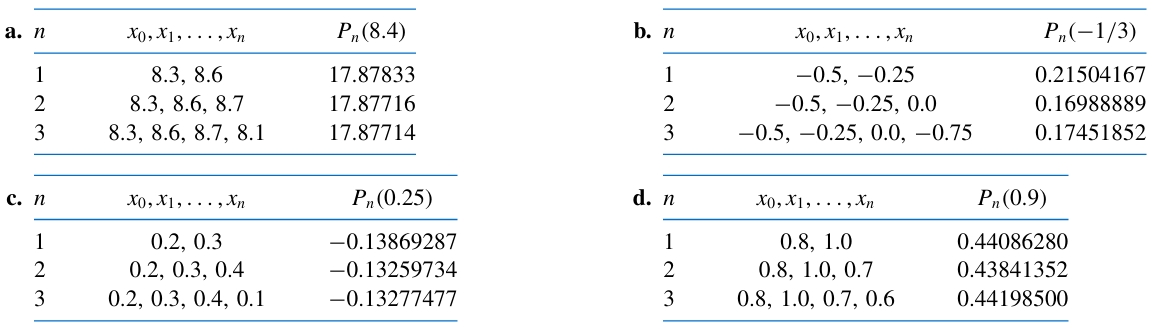
\includegraphics[width=15cm]{CompQuizMod3Sec1}
\end{center}
\end{mysolution}
\end{myexercise}

\section{Divided Differences}

\begin{youtube}
This videos presents a discussion on divided differences. Follow the discussion and then solve the problems in the subsequent quiz.

\end{youtube}
\mylink{https://www.youtube.com/watch?\\v=BAwOGkchq7w\&list=PLDea8VeK4MUTppAXQzHBNz3KiyEd9SQms\&index=66}

\mylink{https://www.youtube.com/watch?\\v=A8rFozfIWmg\&list=PLDea8VeK4MUTppAXQzHBNz3KiyEd9SQms\&index=67}

\mylink{https://www.youtube.com/watch?v=h-\\MO4BnQWHs\&list=PLDea8VeK4MUTppAXQzHBNz3KiyEd9SQms\&index=68}

\mylink{https://www.youtube.com/watch?v=xVA-\\C1hHu1o\&list=PLDea8VeK4MUTppAXQzHBNz3KiyEd9SQms\&index=69}

\begin{myexercise}%\label{Comprehensionquiz2}
Use 
\[P_n(x)=f[x_0]+\sum^n_{k=1}f[x_0, x_1, \ldots, x_k](x-x_0)\cdots(x-x_{k-1})\]
to construct interpolating polynomials of degree one, two, and three for the following data. Approximate the specified value using each of the polynomials.
\begin{enumerate}[label=(\alph*)]
\item $f(8.4)$ if $f(8.1)=16.94410$, $f(8.3)=17.56492$, $f(8.6)=18.50515$, $f(8.7)=18.82091$
\item $f(0.9)$ if $f(0.6)=-0.17694460$, $f(0.7)=0.01375227$, $f(0.8)=0.22363362$, $f(1.0)=0.65809197$
\end{enumerate}
\begin{mysolution}
\begin{enumerate}[label=(\alph*)]
\item $P_1(x) = 16.9441 +3.1041(x -8.1)$; $P_1(8.4) = 17.87533$, $P_2(x) = P_1(x) + 0.06(x - 8.1)(x - 8.3)$; $P_2(8.4) = 17.87713$, $P_3(x) = P_2(x)-0.00208333(x- 8.1)(x - 8.3)(x-8.6)$; $P_3(8.4) = 17.87714$
\item $P_1(x) =-0.1769446 +1.9069687(x-0.6)$; $P1(0.9) = 0.395146$, $P_2(x) = P_1(x) +0.959224(x-0.6)(x-0.7)$; $P_2(0.9) = 0.4526995$, $P_3(x) = P_2(x)-1.785741(x-0.6)(x-0.7)(x-0.8)$; $P_3(0.9) = 0.4419850$
\end{enumerate}
\end{mysolution}
\end{myexercise}



\section{Hermite Interpolation}
\videolesson
\begin{selfvideo}[2]
%LESSON 3: 
This video presents a discussion on Hermite interpolation. Follow the discussion and then solve the problems in the subsequent quiz.
\end{selfvideo}
%\activities
%Read on Hermite interpolation in pages \textcolor{red}{\bf page $136-142$} of the following reference and then attempt the subsequent quiz
%\begin{activity}[\cg Reading]
%\begin{enumerate}
%\item Burden, R. L., Faires, J. D., Burden, A. M. (2015). Numerical Analysis. Tenth Edition, Cengage Learning.\\
%\end{enumerate}
%\end{activity}


\begin{definition}
 Let $x_0, x_1, \ldots, x_n$ be $n + 1$ distinct numbers in $[a,b]$ and for $i = 0, 1, \ldots, n$ let $m_i$ be a  nonnegative integer. Suppose that $f\in C^m[a,b]$, where $m =\max_{0\leq i\leq n} m_i$. The {\bf osculating polynomial} approximating $f$ is the polynomial $P(x)$ of least degree such that
\[\frac{d^kP(x_i)}{dx^k}=\frac{d^kf(x_i)}{dx^k},\quad\mbox{for each} i = 0, 1, \ldots, n\quad \mbox{and}\quad k = 0, 1, \ldots, m_i.\]
\end{definition}

Note that when $n = 0$, the osculating polynomial approximating $f$ is the $m_0$th Taylor polynomial for $f$ at $x_0$. When $m_i = 0$ for each $i$, the osculating polynomial is the $n$th Lagrange polynomial interpolating $f$ on $x_0, x_1, \ldots, x_n$

\subsection*{ Hermite Polynomials}\label{thm:hermite1}
The case when $m_i = 1$, for each $i = 0, 1, \ldots, n$, gives the {\bf Hermite polynomials}. For a given function $f$, these polynomials agree with $f$ at $x_0, x_1, \ldots, x_n$. In addition, since their first derivatives agree with those of $f$, they have the same ``shape'' as the function at $(x_i, f(x_i))$ in the sense that the tangent lines to the polynomial and the function agree. We will restrict our study of osculating polynomials to this situation and consider first a theorem that describes precisely the form of the Hermite polynomials.

\begin{theorem}\label{Hermitthm1}
If $f \in C^{1}[a, b]$ and $x_{0}, \ldots, x_{n} \in[a, b]$ are distinct, the unique polynomial of least degree agreeing with $f$ and $f^{\prime}$ at $x_{0}, \ldots, x_{n}$ is the Hermite polynomial of degree at most $2 n+1$ given by

$$
H_{2 n+1}(x)=\sum_{j=0}^{n} f\left(x_{j}\right) H_{n, j}(x)+\sum_{j=0}^{n} f^{\prime}\left(x_{j}\right) \hat{H}_{n, j}(x),
$$

%Hermite gave a description of a general osculatory polynomial in a letter to Carl W. Borchardt in 1878, to whom he regularly sent his new results. His demonstration is an interesting application of the use of complex integration techniques to solve a real-valued problem.\\
where, for $L_{n, j}(x)$ denoting the $j$ th Lagrange coefficient polynomial of degree $n$, we have

$$
H_{n, j}(x)=\left[1-2\left(x-x_{j}\right) L_{n, j}^{\prime}\left(x_{j}\right)\right] L_{n, j}^{2}(x) \quad \text { and } \quad \hat{H}_{n, j}(x)=\left(x-x_{j}\right) L_{n, j}^{2}(x) .
$$

Moreover, if $f \in C^{2 n+2}[a, b]$, then

$$
f(x)=H_{2 n+1}(x)+\frac{\left(x-x_{0}\right)^{2} \ldots\left(x-x_{n}\right)^{2}}{(2 n+2)!} f^{(2 n+2)}(\xi(x)),
$$

for some (generally unknown) $\xi(x)$ in the interval $(a, b)$.
\end{theorem}

%Proof First recall that
%
%$$
%L_{n, j}\left(x_{i}\right)= \begin{cases}0, & \text { if } i \neq j \\ 1, & \text { if } i=j\end{cases}
%$$
%
%Hence when $i \neq j$,
%
%$$
%H_{n, j}\left(x_{i}\right)=0 \quad \text { and } \quad \hat{H}_{n, j}\left(x_{i}\right)=0,
%$$
%
%whereas, for each $i$,
%
%$$
%H_{n, i}\left(x_{i}\right)=\left[1-2\left(x_{i}-x_{i}\right) L_{n, i}^{\prime}\left(x_{i}\right)\right] \cdot 1=1 \quad \text { and } \quad \hat{H}_{n, i}\left(x_{i}\right)=\left(x_{i}-x_{i}\right) \cdot 1^{2}=0 .
%$$
%
%As a consequence
%
%$$
%H_{2 n+1}\left(x_{i}\right)=\sum_{\substack{j=0 \\ j \neq i}}^{n} f\left(x_{j}\right) \cdot 0+f\left(x_{i}\right) \cdot 1+\sum_{j=0}^{n} f^{\prime}\left(x_{j}\right) \cdot 0=f\left(x_{i}\right),
%$$
%
%so $H_{2 n+1}$ agrees with $f$ at $x_{0}, x_{1}, \ldots, x_{n}$.\\
%To show the agreement of $H_{2 n+1}^{\prime}$ with $f^{\prime}$ at the nodes, first note that $L_{n, j}(x)$ is a factor of $H_{n, j}^{\prime}(x)$, so $H_{n, j}^{\prime}\left(x_{i}\right)=0$ when $i \neq j$. In addition, when $i=j$ we have $L_{n, i}\left(x_{i}\right)=1$, so
%
%$$
%\begin{aligned}
%H_{n, i}^{\prime}\left(x_{i}\right) & =-2 L_{n, i}^{\prime}\left(x_{i}\right) \cdot L_{n, i}^{2}\left(x_{i}\right)+\left[1-2\left(x_{i}-x_{i}\right) L_{n, i}^{\prime}\left(x_{i}\right)\right] 2 L_{n, i}\left(x_{i}\right) L_{n, i}^{\prime}\left(x_{i}\right) \\
%& =-2 L_{n, i}^{\prime}\left(x_{i}\right)+2 L_{n, i}^{\prime}\left(x_{i}\right)=0
%\end{aligned}
%$$
%
%Hence, $H_{n, j}^{\prime}\left(x_{i}\right)=0$ for all $i$ and $j$.\\
%Finally,
%
%$$
%\begin{aligned}
%\hat{H}_{n, j}^{\prime}\left(x_{i}\right) & =L_{n, j}^{2}\left(x_{i}\right)+\left(x_{i}-x_{j}\right) 2 L_{n, j}\left(x_{i}\right) L_{n, j}^{\prime}\left(x_{i}\right) \\
%& =L_{n, j}\left(x_{i}\right)\left[L_{n, j}\left(x_{i}\right)+2\left(x_{i}-x_{j}\right) L_{n, j}^{\prime}\left(x_{i}\right)\right],
%\end{aligned}
%$$
%
%so $\hat{H}_{n, j}^{\prime}\left(x_{i}\right)=0$ if $i \neq j$ and $\hat{H}_{n, i}^{\prime}\left(x_{i}\right)=1$. Combining these facts, we have
%
%$$
%H_{2 n+1}^{\prime}\left(x_{i}\right)=\sum_{j=0}^{n} f\left(x_{j}\right) \cdot 0+\sum_{\substack{j=0 \\ j \neq i}}^{n} f^{\prime}\left(x_{j}\right) \cdot 0+f^{\prime}\left(x_{i}\right) \cdot 1=f^{\prime}\left(x_{i}\right) .
%$$
%
%Therefore, $H_{2 n+1}$ agrees with $f$ and $H_{2 n+1}^{\prime}$ with $f^{\prime}$ at $x_{0}, x_{1}, \ldots, x_{n}$.\\
%The uniqueness of this polynomial and the error formula are considered in Exercise 11.
%
\begin{example}\label{exam:hermite1}
Use the Hermite polynomial that agrees with the data listed in Table \ref{tab:hermiteexample1} to find an approximation of $f(1.5)$.
\end{example}
%Table 3.15

\begin{table}
\centering
\begin{tabular}{cccc}
\hline
$k$ & $x_{k}$ & $f\left(x_{k}\right)$ & $f^{\prime}\left(x_{k}\right)$ \\
\hline
0 & 1.3 & 0.6200860 & -0.5220232 \\
1 & 1.6 & 0.4554022 & -0.5698959 \\
2 & 1.9 & 0.2818186 & -0.5811571 \\
\hline
\end{tabular}
\caption{\scriptsize Table $8$}
\label{tab:hermiteexample1}
\end{table}

\begin{mysolution}
We first compute the Lagrange polynomials and their derivatives. This gives

$$
\begin{aligned}
& L_{2,0}(x)=\frac{\left(x-x_{1}\right)\left(x-x_{2}\right)}{\left(x_{0}-x_{1}\right)\left(x_{0}-x_{2}\right)}=\frac{50}{9} x^{2}-\frac{175}{9} x+\frac{152}{9}, \quad L_{2,0}^{\prime}(x)=\frac{100}{9} x-\frac{175}{9} ; \\
& L_{2,1}(x)=\frac{\left(x-x_{0}\right)\left(x-x_{2}\right)}{\left(x_{1}-x_{0}\right)\left(x_{1}-x_{2}\right)}=\frac{-100}{9} x^{2}+\frac{320}{9} x-\frac{247}{9}, \quad L_{2,1}^{\prime}(x)=\frac{-200}{9} x+\frac{320}{9} ;
\end{aligned}
$$

and

$$
L_{2,2}=\frac{\left(x-x_{0}\right)\left(x-x_{1}\right)}{\left(x_{2}-x_{0}\right)\left(x_{2}-x_{1}\right)}=\frac{50}{9} x^{2}-\frac{145}{9} x+\frac{104}{9}, \quad \quad L_{2,2}^{\prime}(x)=\frac{100}{9} x-\frac{145}{9} .
$$

The polynomials $H_{2, j}(x)$ and $\hat{H}_{2, j}(x)$ are then

$$
\begin{aligned}
H_{2,0}(x) & =[1-2(x-1.3)(-5)]\left(\frac{50}{9} x^{2}-\frac{175}{9} x+\frac{152}{9}\right)^{2} \\
& =(10 x-12)\left(\frac{50}{9} x^{2}-\frac{175}{9} x+\frac{152}{9}\right)^{2} \\
H_{2,1}(x) & =1 \cdot\left(\frac{-100}{9} x^{2}+\frac{320}{9} x-\frac{247}{9}\right)^{2} \\
H_{2,2}(x) & =10(2-x)\left(\frac{50}{9} x^{2}-\frac{145}{9} x+\frac{104}{9}\right)^{2} \\
\hat{H}_{2,0}(x) & =(x-1.3)\left(\frac{50}{9} x^{2}-\frac{175}{9} x+\frac{152}{9}\right)^{2} \\
\hat{H}_{2,1}(x) & =(x-1.6)\left(\frac{-100}{9} x^{2}+\frac{320}{9} x-\frac{247}{9}\right)^{2}
\end{aligned}
$$

and

$$
\hat{H}_{2,2}(x)=(x-1.9)\left(\frac{50}{9} x^{2}-\frac{145}{9} x+\frac{104}{9}\right)^{2}
$$

Finally

$$
\begin{aligned}
H_{5}(x)= & 0.6200860 H_{2,0}(x)+0.4554022 H_{2,1}(x)+0.2818186 H_{2,2}(x) \\
& -0.5220232 \hat{H}_{2,0}(x)-0.5698959 \hat{H}_{2,1}(x)-0.5811571 \hat{H}_{2,2}(x)
\end{aligned}
$$

and

$$
\begin{aligned}
H_{5}(1.5)= & 0.6200860\left(\frac{4}{27}\right)+0.4554022\left(\frac{64}{81}\right)+0.2818186\left(\frac{5}{81}\right) \\
& -0.5220232\left(\frac{4}{405}\right)-0.5698959\left(\frac{-32}{405}\right)-0.5811571\left(\frac{-2}{405}\right) \\
= & 0.5118277
\end{aligned}
$$

a result that is accurate to the places listed.
\end{mysolution}

Although Theorem \ref{thm:hermite1} provides a complete description of the Hermite polynomials, it is clear from Example \ref{exam:hermite1} that the need to determine and evaluate the Lagrange polynomials and their derivatives makes the procedure tedious even for small values of $n$.

\subsection*{Hermite Polynomials Using Divided Differences}
There is an alternative method for generating Hermite approximations that has as its basis the Newton interpolatory divided-difference formula at $x_{0}, x_{1}, \ldots, x_{n}$, given by

$$
P_{n}(x)=f\left[x_{0}\right]+\sum_{k=1}^{n} f\left[x_{0}, x_{1}, \ldots, x_{k}\right]\left(x-x_{0}\right) \cdots\left(x-x_{k-1}\right)
$$
The alternative method uses the connection between the $n$th divided difference and the $n$th derivative of $f$.

Suppose that the distinct numbers $x_{0}, x_{1}, \ldots, x_{n}$ are given together with the values of $f$ and $f^{\prime}$ at these numbers. Define a new sequence $z_{0}, z_{1}, \ldots, z_{2 n+1}$ by

$$
z_{2 i}=z_{2 i+1}=x_{i}, \quad \text { for each } i=0,1, \ldots, n,
$$
and construct the divided difference table in the form of Table 3.9 that uses $z_{0}, z_{1}, \ldots, z_{2 n+1}$.

Since $z_{2 i}=z_{2 i+1}=x_{i}$ for each $i$, we cannot define $f\left[z_{2 i}, z_{2 i+1}\right]$ by the divided difference formula. However, if we assume, based on Theorem 3.6, that the reasonable substitution in this situation is $f\left[z_{2 i}, z_{2 i+1}\right]=f^{\prime}\left(z_{2 i}\right)=f^{\prime}\left(x_{i}\right)$, we can use the entries

$$
f^{\prime}\left(x_{0}\right), f^{\prime}\left(x_{1}\right), \ldots, f^{\prime}\left(x_{n}\right)
$$
in place of the undefined first divided differences

$$
f\left[z_{0}, z_{1}\right], f\left[z_{2}, z_{3}\right], \ldots, f\left[z_{2 n}, z_{2 n+1}\right] .
$$

The remaining divided differences are produced as usual, and the appropriate divided differences are employed in Newton's interpolatory divided-difference formula. Table \ref{tab:hermite2} shows the entries that are used for the first three divided-difference columns when determining the Hermite polynomial $H_{5}(x)$ for $x_{0}, x_{1}$, and $x_{2}$. The remaining entries are generated in the same manner as in Table \ref{tab:hermite2}. The Hermite polynomial is then given by

$$
H_{2 n+1}(x)=f\left[z_{0}\right]+\sum_{k=1}^{2 n+1} f\left[z_{0}, \ldots, z_{k}\right]\left(x-z_{0}\right)\left(x-z_{1}\right) \cdots\left(x-z_{k-1}\right)
$$

%A proof of this fact can be found in [Pow], p. 56.
%
%Table 3.16

\begin{table}
\centering
\begin{tabular}{|l|l|l|l|}
\hline
$z$ & $f(z)$ & First divided differences & Second divided differences \\
\hline
$z_{0}=x_{0}$ & $f\left[z_{0}\right]=f\left(x_{0}\right)$ &  &  \\
\hline
 &  & $f\left[z_{0}, z_{1}\right]=f^{\prime}\left(x_{0}\right)$ &  \\
\hline
$z_{1}=x_{0}$ & $f\left[z_{1}\right]=f\left(x_{0}\right)$ &  & $f\left[z_{0}, z_{1}, z_{2}\right]=\frac{f\left[z_{1}, z_{2}\right]-f\left[z_{0}, z_{1}\right]}{z_{2}-z_{0}}$ \\
\hline
 &  & $f\left[z_{1}, z_{2}\right]=\frac{f\left[z_{2}\right]-f\left[z_{1}\right]}{z_{2}-z_{1}}$ &  \\
\hline
$z_{2}=x_{1}$ & $f\left[z_{2}\right]=f\left(x_{1}\right)$ &  & $f\left[z_{1}, z_{2}, z_{3}\right]=\frac{f\left[z_{2}, z_{3}\right]-f\left[z_{1}, z_{2}\right]}{z_{3}-z_{1}}$ \\
\hline
 &  & $f\left[z_{2}, z_{3}\right]=f^{\prime}\left(x_{1}\right)$ &  \\
\hline
$z_{3}=x_{1}$ & $f\left[z_{3}\right]=f\left(x_{1}\right)$ &  & $f\left[z_{2}, z_{3}, z_{4}\right]=\frac{f\left[z_{3}, z_{4}\right]-f\left[z_{2}, z_{3}\right]}{z_{4}-z_{2}}$ \\
\hline
 &  & $f\left[z_{3}, z_{4}\right]=\frac{f\left[z_{4}\right]-f\left[z_{3}\right]}{z_{4}-z_{3}}$ &  \\
\hline
$z_{4}=x_{2}$ & $f\left[z_{4}\right]=f\left(x_{2}\right)$ &  & $f\left[z_{3}, z_{4}, z_{5}\right]=\frac{f\left[z_{4}, z_{5}\right]-f\left[z_{3}, z_{4}\right]}{z_{5}-z_{3}}$ \\
\hline
 &  & $f\left[z_{4}, z_{5}\right]=f^{\prime}\left(x_{2}\right)$ &  \\
\hline
$z_{5}=x_{2}$ & $f\left[z_{5}\right]=f\left(x_{2}\right)$ &  &  \\
\hline
\end{tabular}
\caption{\scriptsize Table $9$}
\label{tab:hermite2}
\end{table}

\begin{example}
Use the data given in Example 1 and the divided difference method to determine the Hermite polynomial approximation at $x=1.5$.
\end{example}

\begin{mysolution}The underlined entries in the first three columns of Table \ref{tab:hermiteexample2} are the data given in Example \ref{exam:hermite1}. The remaining entries in this table are generated by the standard divided difference formula relative to $x_i, x_{i+1}, \ldots, x_{i+k}$ given by
\[f[x_i, x_{i+1}, \ldots, x_{i+k}]=\frac{f[x_i, x_{i+1}, \ldots, x_{i+k}]-f[x_1, x_{i+1}, \ldots, x_{i+k-1}]}{x_{i+k}-x_1}\]

For example, for the second entry in the third column we use the second $1.3$ entry in the second column and the first $1.6$ entry in that column to obtain

$$
\frac{0.4554022-0.6200860}{1.6-1.3}=-0.5489460 .
$$
For the first entry in the fourth column we use the first $1.3$ entry in the third column and the first $1.6$ entry in that column to obtain

$$
\frac{-0.5489460-(-0.5220232)}{1.6-1.3}=-0.0897427 .
$$
The value of the Hermite polynomial at $1.5$ is

$$
\begin{aligned}
H_{5}(1.5)= & f[1.3]+f^{\prime}(1.3)(1.5-1.3)+f[1.3,1.3,1.6](1.5-1.3)^{2} \\
& +f[1.3,1.3,1.6,1.6](1.5-1.3)^{2}(1.5-1.6) \\
& +f[1.3,1.3,1.6,1.6,1.9](1.5-1.3)^{2}(1.5-1.6)^{2} \\
& +f[1.3,1.3,1.6,1.6,1.9,1.9](1.5-1.3)^{2}(1.5-1.6)^{2}(1.5-1.9) \\
= & 0.6200860+(-0.5220232)(0.2)+(-0.0897427)(0.2)^{2} \\
& +0.0663657(0.2)^{2}(-0.1)+0.0026663(0.2)^{2}(-0.1)^{2} \\
& +(-0.0027738)(0.2)^{2}(-0.1)^{2}(-0.4) \\
= & 0.5118277
\end{aligned}
$$
\end{mysolution}
%Table 3.17
%
\begin{table}
\centering
\begin{tabular}{|l|l|l|l|l|l|l|}
\hline
1.3 & 0.6200860 & \multicolumn{5}{|c|}{} \\
\hline
 &  & -0.5220232 &  & \multirow[b]{3}{*}{0.0663657} & \multirow{3}{*}{} & \multirow{3}{*}{} \\
\hline
$\underline{1.3}$ & 0.6200860 &  & -0.0897427 &  &  &  \\
\hline
 &  & -0.5489460 & \multirow[b]{2}{*}{-0.0698330} &  &  &  \\
\hline
1.6 & 0.4554022 &  &  & \multicolumn{3}{|c|}{0.0026663} \\
\hline
\multicolumn{2}{|c|}{} & -0.5698959 & \multirow[b]{2}{*}{-0.0290537} & 0.0679655 & \multicolumn{2}{|r|}{-0.0027738} \\
\hline
1.6 & 0.4554022 & \multirow[b]{2}{*}{-0.5786120} &  &  & 0.0010020 &  \\
\hline
\multicolumn{2}{|c|}{} &  &  & 0.0685667 &  &  \\
\hline
1.9 & 0.2818186 & \multirow[b]{2}{*}{-0.5811571} & -0.0084837 &  &  &  \\
\hline
\multicolumn{2}{|c|}{} &  &  &  &  &  \\
\hline
1.9 & 0.2818186 &  &  &  &  &  \\
\hline
\end{tabular}
\caption{\scriptsize Table $10$}
\label{tab:hermiteexample2}
\end{table}


\begin{myexercise}%\label{Comprehensionquiz2}
Use Theorem \ref{Hermitthm1} to construct an approximating polynomial for the following data.
\begin{enumerate}[label=(\alph*)]
\item
\begin{center}
\begin{tabular}{c|c|c}
$x$ & $f(x)$ & $f^{\prime}(x)$ \\
\hline
8.3 & 17.56492 & 3.116256 \\
8.6 & 18.50515 & 3.151762 \\
\end{tabular}
\end{center}

\item
\begin{center}
\begin{tabular}{c|c|c}
$x$ & $f(x)$ & $f^{\prime}(x)$ \\
\hline
0.8 & 0.22363362 & 2.1691753 \\
1.0 & 0.65809197 & 2.0466965 \\
\end{tabular}
\end{center}

\item
\begin{center}
\begin{tabular}{l|r|c}
\multicolumn{1}{c|}{$x$} & \multicolumn{1}{c|}{$f(x)$} & $f^{\prime}(x)$ \\
\hline
-0.5 & -0.0247500 & 0.7510000 \\
-0.25 & 0.3349375 & 2.1890000 \\
0 & 1.1010000 & 4.0020000 \\
\end{tabular}
\end{center}

\item
\begin{center}
\begin{tabular}{c|r|c}
$x$ & \multicolumn{1}{|c|}{$f(x)$} & \multicolumn{1}{c}{$f^{\prime}(x)$} \\
\hline
0.1 & -0.62049958 & 3.58502082 \\
0.2 & -0.28398668 & 3.14033271 \\
0.3 & 0.00660095 & 2.66668043 \\
0.4 & 0.24842440 & 2.16529366 \\
\end{tabular}
\end{center}
\end{enumerate}

\begin{mysolution}
The coefficients for the polynomials in divided-difference form are given in the following tables. For example, the polynomial in part (a) is
\[\begin{split}
H_3(x)=&17.56492+3.116256(x-8.3)+0.05948(x-8.3)^2-\\
&0.00202222(x-8.3)^2(x-8.6).
\end{split}\]
\begin{center}
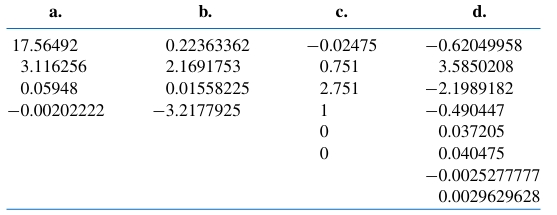
\includegraphics[width=12cm]{CompQuizMod3Sec3Sol}
\end{center}
\end{mysolution}
\end{myexercise}

\section{Cubic Spline Interpolation}
\begin{youtube}
This video presents a discussion on cubic spline interpolation. Follow the discussion and then solve the problems in the subsequent quiz.
\end{youtube}

\mylink{https://www.youtube.com/watch?\\v=pBtqaK0PzrA\&list=PLDea8VeK4MUTppAXQzHBNz3KiyEd9SQms\&index=77}

\mylink{https://www.youtube.com/watch?\\v=yOUst2672qo\&list=PLDea8VeK4MUTppAXQzHBNz3KiyEd9SQms\&index=78}

\mylink{https://www.youtube.com/watch?\\v=\_6\_z7DzDhUo\&list=PLDea8VeK4MUTppAXQzHBNz3KiyEd9SQms\&index=79}

%\videolesson
%\begin{selfvideo}[2]
%%LESSON 3: 
%This video presents a discussion on cubic spline interpolation. Follow the discussion and then solve the problems in the subsequent quiz.
%\end{selfvideo}
%\begin{boxB}Question: \end{boxB}
%The previous sections concerned the approximation of arbitrary functions on closed intervals using a single polynomial. However, high-degree polynomials can oscillate erratically, that is, a minor fluctuation over a small portion of the interval can induce large fluctuations over the entire range. 
%
%An alternative approach is to divide the approximation interval into a collection of subintervals and construct a (generally) different approximating polynomial on each subinterval. This is called {\bf piecewise-polynomial approximation}.
%
%\subsection*{Piecewise-Polynomial Approximation}
%The simplest piecewise-polynomial approximation is {\bf piecewise-linear} interpolation, which consists of joining a set of data points
%\[\left\{\left(x_{0}, f\left(x_{0}\right)\right),\left(x_{1}, f\left(x_{1}\right)\right), \ldots,\left(x_{n}, f\left(x_{n}\right)\right)\right\}\]
%by a series of straight lines, as shown in Figure \ref{fig:piecewiselinapproxpic1}
%\begin{figure}[h]
%\centering
%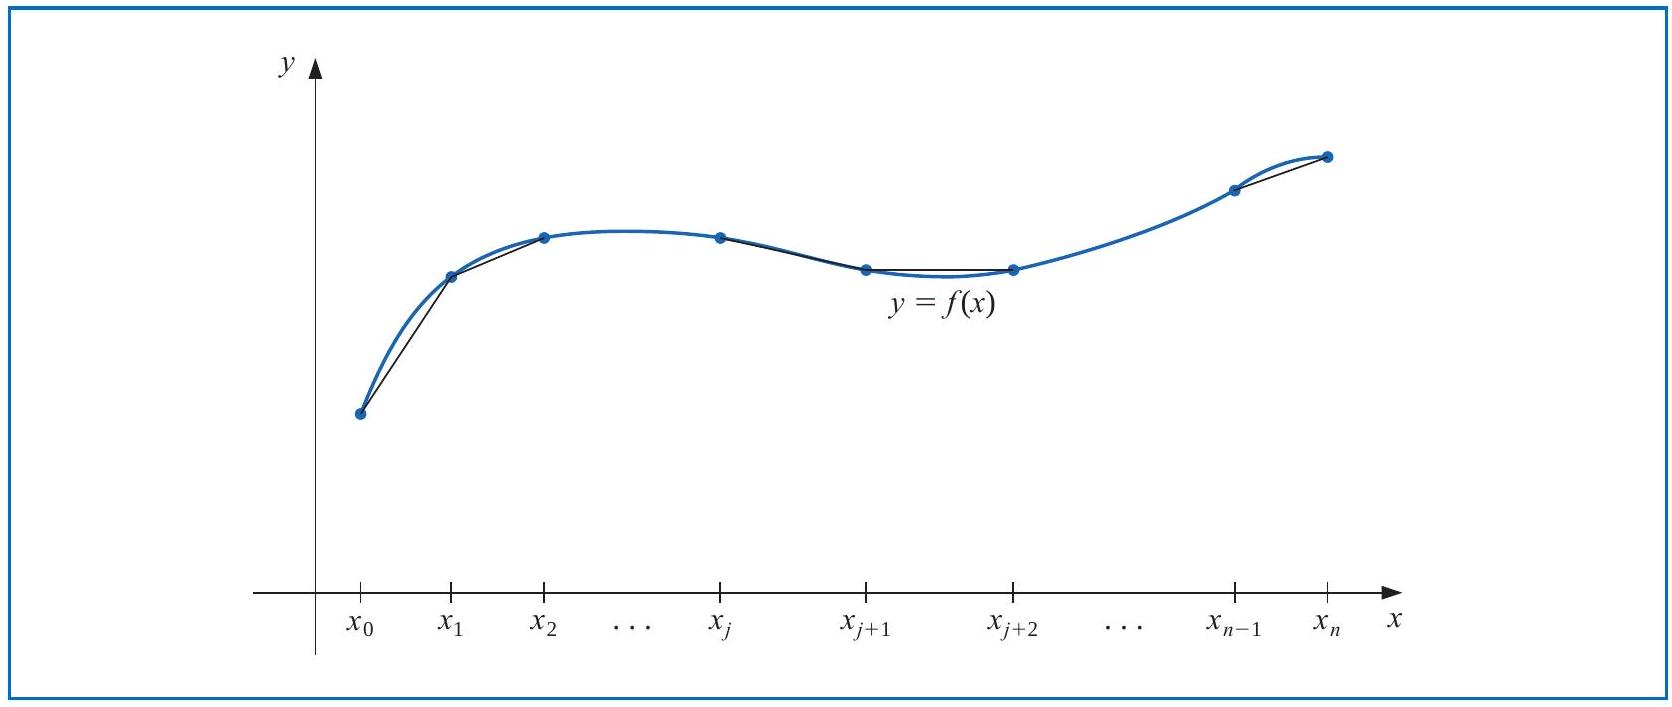
\includegraphics[width=9cm]{piecewiselinapproxpic1.JPG}
%\caption{}
%\label{fig:piecewiselinapproxpic1}
%\end{figure}
%
%A disadvantage of linear function approximation is that there is likely no differentiability at the endpoints of the subintervals, which, in a geometrical context, means that the interpolating function is not "smooth." Often it is clear from physical conditions that smoothness is required, so the approximating function must be continuously differentiable.
%
%An alternative procedure is to use a piecewise polynomial of Hermite type. For example, if the values of $f$ and of $f^{\prime}$ are known at each of the points $x_{0}<x_{1}<\cdots<x_{n}$, a cubic Hermite polynomial can be used on each of the subintervals $\left[x_{0}, x_{1}\right],\left[x_{1}, x_{2}\right], \ldots,\left[x_{n-1}, x_{n}\right]$ to obtain a function that has a continuous derivative on the interval $\left[x_{0}, x_{n}\right]$.\\
%${ }^{1}$.
%%
%%Figure 3.7\\
%
%%
%%Isaac Jacob Schoenberg (1903-1990) developed his work on splines during World War II while on leave from the University of Pennsylvania to work at the Army's Ballistic\\
%%Research Laboratory in Aberdeen, Maryland. His original work involved numerical procedures for solving differential equations. The much broader application of splines to the areas of data fitting and computer-aided geometric design became evident with the widespread availability of computers in the 1960s.
%
%To determine the appropriate Hermite cubic polynomial on a given interval is simply a matter of computing $H_{3}(x)$ for that interval. The Lagrange interpolating polynomials needed to determine $H_{3}$ are of first degree, so this can be accomplished without great difficulty. However, to use Hermite piecewise polynomials for general interpolation, we need to know the derivative of the function being approximated, and this is frequently unavailable.
%
%The remainder of this section considers approximation using piecewise polynomials that require no specific derivative information, except perhaps at the endpoints of the interval on which the function is being approximated.
%
%The simplest type of differentiable piecewise-polynomial function on an entire interval $\left[x_{0}, x_{n}\right]$ is the function obtained by fitting one quadratic polynomial between each successive pair of nodes. This is done by constructing a quadratic on $\left[x_{0}, x_{1}\right]$ agreeing with the function at $x_{0}$ and $x_{1}$, another quadratic on $\left[x_{1}, x_{2}\right]$ agreeing with the function at $x_{1}$ and $x_{2}$, and so on. A general quadratic polynomial has three arbitrary constants-the constant term, the coefficient of $x$, and the coefficient of $x^{2}$-and only two conditions are required to fit the data at the endpoints of each subinterval. So flexibility exists that permits the quadratics to be chosen so that the interpolant has a continuous derivative on $\left[x_{0}, x_{n}\right]$. The difficulty arises because we generally need to specify conditions about the derivative of the interpolant at the endpoints $x_{0}$ and $x_{n}$. There is not a sufficient number of constants to ensure that the conditions will be satisfied.
%
%\subsection*{Cubic Splines}
%The most common piecewise-polynomial approximation uses cubic polynomials between each successive pair of nodes and is called {\bf cubic spline interpolation}. A general cubic polynomial involves four constants, so there is sufficient flexibility in the cubic spline procedure to ensure that the interpolant is not only continuously differentiable on the interval, but also has a continuous second derivative. The construction of the cubic spline does not, however, assume that the derivatives of the interpolant agree with those of the function it is approximating, even at the nodes. (See Figure 3.8.)
%
%Figure 3.8\\
%\includegraphics[max width=\textwidth, center]{2025_05_15_4109a88b43049bd640d1g-42(1)}
%
%Definition 3.10
%
%A natural spline has no conditions imposed for the direction at its endpoints, so the curve takes the shape of a straight line after it passes through the interpolation points nearest its endpoints. The name derives from the fact that this is the natural shape a flexible strip assumes if forced to pass through specified interpolation points with no additional constraints. (See Figure 3.9.)\\
%\includegraphics[max width=\textwidth, center]{2025_05_15_4109a88b43049bd640d1g-42}
%
%Figure 3.9
%
%Given a function $f$ defined on $[a, b]$ and a set of nodes $a=x_{0}<x_{1}<\cdots<$ $x_{n}=b$, a cubic spline interpolant $S$ for $f$ is a function that satisfies the following conditions:\\
%(a) $\quad S(x)$ is a cubic polynomial, denoted $S_{j}(x)$, on the subinterval $\left[x_{j}, x_{j+1}\right]$ for each $j=0,1, \ldots, n-1 ;$\\
%(b) $\quad S_{j}\left(x_{j}\right)=f\left(x_{j}\right)$ and $S_{j}\left(x_{j+1}\right)=f\left(x_{j+1}\right)$ for each $j=0,1, \ldots, n-1$;\\
%(c) $S_{j+1}\left(x_{j+1}\right)=S_{j}\left(x_{j+1}\right)$ for each $j=0,1, \ldots, n-2$; (Implied by (b).)\\
%(d) $\quad S_{j+1}^{\prime}\left(x_{j+1}\right)=S_{j}^{\prime}\left(x_{j+1}\right)$ for each $j=0,1, \ldots, n-2$;\\
%(e) $S_{j+1}^{\prime \prime}\left(x_{j+1}\right)=S_{j}^{\prime \prime}\left(x_{j+1}\right)$ for each $j=0,1, \ldots, n-2$;\\
%(f) One of the following sets of boundary conditions is satisfied:\\
%(i) $\quad S^{\prime \prime}\left(x_{0}\right)=S^{\prime \prime}\left(x_{n}\right)=0 \quad$ (natural (or free) boundary);\\
%(ii) $\quad S^{\prime}\left(x_{0}\right)=f^{\prime}\left(x_{0}\right)$ and $\quad S^{\prime}\left(x_{n}\right)=f^{\prime}\left(x_{n}\right) \quad$ (clamped boundary).
%
%Although cubic splines are defined with other boundary conditions, the conditions given in (f) are sufficient for our purposes. When the free boundary conditions occur, the spline is called a natural spline, and its graph approximates the shape that a long flexible rod would assume if forced to go through the data points $\left\{\left(x_{0}, f\left(x_{0}\right)\right),\left(x_{1}, f\left(x_{1}\right)\right), \ldots,\left(x_{n}, f\left(x_{n}\right)\right)\right\}$.
%
%In general, clamped boundary conditions lead to more accurate approximations because they include more information about the function. However, for this type of boundary condition to hold, it is necessary to have either the values of the derivative at the endpoints or an accurate approximation to those values.
%
%Example 1 Construct a natural cubic spline that passes through the points $(1,2),(2,3)$, and $(3,5)$.\\[0pt]
%Solution This spline consists of two cubics. The first for the interval [1, 2], denoted
%
%$$
%S_{0}(x)=a_{0}+b_{0}(x-1)+c_{0}(x-1)^{2}+d_{0}(x-1)^{3},
%$$
%
%Clamping a spline indicates that the ends of the flexible strip are fixed so that it is forced to take a specific direction at each of its endpoints. This is important, for example, when two spline functions should match at their endpoints. This is done mathematically by specifying the values of the derivative of the curve at the endpoints of the spline.\\[0pt]
%and the other for [2,3], denoted
%
%$$
%S_{1}(x)=a_{1}+b_{1}(x-2)+c_{1}(x-2)^{2}+d_{1}(x-2)^{3} .
%$$
%
%There are 8 constants to be determined, which requires 8 conditions. Four conditions come from the fact that the splines must agree with the data at the nodes. Hence
%
%$$
%\begin{aligned}
%& 2=f(1)=a_{0}, \quad 3=f(2)=a_{0}+b_{0}+c_{0}+d_{0}, \quad 3=f(2)=a_{1}, \quad \text { and } \\
%& 5=f(3)=a_{1}+b_{1}+c_{1}+d_{1} .
%\end{aligned}
%$$
%
%Two more come from the fact that $S_{0}^{\prime}(2)=S_{1}^{\prime}(2)$ and $S_{0}^{\prime \prime}(2)=S_{1}^{\prime \prime}(2)$. These are
%
%$$
%S_{0}^{\prime}(2)=S_{1}^{\prime}(2): \quad b_{0}+2 c_{0}+3 d_{0}=b_{1} \quad \text { and } \quad S_{0}^{\prime \prime}(2)=S_{1}^{\prime \prime}(2): \quad 2 c_{0}+6 d_{0}=2 c_{1}
%$$
%
%The final two come from the natural boundary conditions:
%
%$$
%S_{0}^{\prime \prime}(1)=0: \quad 2 c_{0}=0 \quad \text { and } \quad S_{1}^{\prime \prime}(3)=0: \quad 2 c_{1}+6 d_{1}=0 .
%$$
%
%Solving this system of equations gives the spline
%
%$$
%S(x)=\left\{\begin{array}{l}
%2+\frac{3}{4}(x-1)+\frac{1}{4}(x-1)^{3}, \text { for } x \in[1,2] \\
%3+\frac{3}{2}(x-2)+\frac{3}{4}(x-2)^{2}-\frac{1}{4}(x-2)^{3}, \text { for } x \in[2,3]
%\end{array}\right.
%$$
%
%\section*{Construction of a Cubic Spline}
%As the preceding example demonstrates, a spline defined on an interval that is divided into $n$ subintervals will require determining $4 n$ constants. To construct the cubic spline interpolant for a given function $f$, the conditions in the definition are applied to the cubic polynomials
%
%$$
%S_{j}(x)=a_{j}+b_{j}\left(x-x_{j}\right)+c_{j}\left(x-x_{j}\right)^{2}+d_{j}\left(x-x_{j}\right)^{3},
%$$
%
%for each $j=0,1, \ldots, n-1$. Since $S_{j}\left(x_{j}\right)=a_{j}=f\left(x_{j}\right)$, condition (c) can be applied to obtain
%
%$$
%a_{j+1}=S_{j+1}\left(x_{j+1}\right)=S_{j}\left(x_{j+1}\right)=a_{j}+b_{j}\left(x_{j+1}-x_{j}\right)+c_{j}\left(x_{j+1}-x_{j}\right)^{2}+d_{j}\left(x_{j+1}-x_{j}\right)^{3},
%$$
%
%for each $j=0,1, \ldots, n-2$.\\
%The terms $x_{j+1}-x_{j}$ are used repeatedly in this development, so it is convenient to introduce the simpler notation
%
%$$
%h_{j}=x_{j+1}-x_{j},
%$$
%
%for each $j=0,1, \ldots, n-1$. If we also define $a_{n}=f\left(x_{n}\right)$, then the equation
%
%
%\begin{equation*}
%a_{j+1}=a_{j}+b_{j} h_{j}+c_{j} h_{j}^{2}+d_{j} h_{j}^{3} \tag{3.15}
%\end{equation*}
%
%
%holds for each $j=0,1, \ldots, n-1$.
%
%In a similar manner, define $b_{n}=S^{\prime}\left(x_{n}\right)$ and observe that
%
%$$
%S_{j}^{\prime}(x)=b_{j}+2 c_{j}\left(x-x_{j}\right)+3 d_{j}\left(x-x_{j}\right)^{2}
%$$
%
%implies $S_{j}^{\prime}\left(x_{j}\right)=b_{j}$, for each $j=0,1, \ldots, n-1$. Applying condition (d) gives
%
%
%\begin{equation*}
%b_{j+1}=b_{j}+2 c_{j} h_{j}+3 d_{j} h_{j}^{2} \tag{3.16}
%\end{equation*}
%
%
%for each $j=0,1, \ldots, n-1$.\\
%Another relationship between the coefficients of $S_{j}$ is obtained by defining $c_{n}=$ $S^{\prime \prime}\left(x_{n}\right) / 2$ and applying condition (e). Then, for each $j=0,1, \ldots, n-1$,
%
%
%\begin{equation*}
%c_{j+1}=c_{j}+3 d_{j} h_{j} \tag{3.17}
%\end{equation*}
%
%
%Solving for $d_{j}$ in Eq. (3.17) and substituting this value into Eqs. (3.15) and (3.16) gives, for each $j=0,1, \ldots, n-1$, the new equations
%
%
%\begin{equation*}
%a_{j+1}=a_{j}+b_{j} h_{j}+\frac{h_{j}^{2}}{3}\left(2 c_{j}+c_{j+1}\right) \tag{3.18}
%\end{equation*}
%
%
%and
%
%
%\begin{equation*}
%b_{j+1}=b_{j}+h_{j}\left(c_{j}+c_{j+1}\right) \tag{3.19}
%\end{equation*}
%
%
%The final relationship involving the coefficients is obtained by solving the appropriate equation in the form of equation (3.18), first for $b_{j}$,
%
%
%\begin{equation*}
%b_{j}=\frac{1}{h_{j}}\left(a_{j+1}-a_{j}\right)-\frac{h_{j}}{3}\left(2 c_{j}+c_{j+1}\right) \tag{3.20}
%\end{equation*}
%
%
%and then, with a reduction of the index, for $b_{j-1}$. This gives
%
%$$
%b_{j-1}=\frac{1}{h_{j-1}}\left(a_{j}-a_{j-1}\right)-\frac{h_{j-1}}{3}\left(2 c_{j-1}+c_{j}\right)
%$$
%
%Substituting these values into the equation derived from Eq. (3.19), with the index reduced by one, gives the linear system of equations
%
%
%\begin{equation*}
%h_{j-1} c_{j-1}+2\left(h_{j-1}+h_{j}\right) c_{j}+h_{j} c_{j+1}=\frac{3}{h_{j}}\left(a_{j+1}-a_{j}\right)-\frac{3}{h_{j-1}}\left(a_{j}-a_{j-1}\right), \tag{3.21}
%\end{equation*}
%
%
%for each $j=1,2, \ldots, n-1$. This system involves only the $\left\{c_{j}\right\}_{j=0}^{n}$ as unknowns. The values of $\left\{h_{j}\right\}_{j=0}^{n-1}$ and $\left\{a_{j}\right\}_{j=0}^{n}$ are given, respectively, by the spacing of the nodes $\left\{x_{j}\right\}_{j=0}^{n}$ and the values of $f$ at the nodes. So once the values of $\left\{c_{j}\right\}_{j=0}^{n}$ are determined, it is a simple matter to find the remainder of the constants $\left\{b_{j}\right\}_{j=0}^{n-1}$ from Eq. (3.20) and $\left\{d_{j}\right\}_{j=0}^{n-1}$ from Eq. (3.17). Then we can construct the cubic polynomials $\left\{S_{j}(x)\right\}_{j=0}^{n-1}$.
%
%The major question that arises in connection with this construction is whether the values of $\left\{c_{j}\right\}_{j=0}^{n}$ can be found using the system of equations given in (3.21) and, if so, whether these values are unique. The following theorems indicate that this is the case when either of the boundary conditions given in part (f) of the definition are imposed. The proofs of these theorems require material from linear algebra, which is discussed in Chapter 6.
%
%\section*{Natural Splines}
%Theorem 3.11 If $f$ is defined at $a=x_{0}<x_{1}<\cdots<x_{n}=b$, then $f$ has a unique natural spline interpolant $S$ on the nodes $x_{0}, x_{1}, \ldots, x_{n}$; that is, a spline interpolant that satisfies the natural boundary conditions $S^{\prime \prime}(a)=0$ and $S^{\prime \prime}(b)=0$.
%
%Proof The boundary conditions in this case imply that $c_{n}=S^{\prime \prime}\left(x_{n}\right) / 2=0$ and that
%
%$$
%0=S^{\prime \prime}\left(x_{0}\right)=2 c_{0}+6 d_{0}\left(x_{0}-x_{0}\right),
%$$
%
%so $c_{0}=0$. The two equations $c_{0}=0$ and $c_{n}=0$ together with the equations in (3.21) produce a linear system described by the vector equation $A \mathbf{x}=\mathbf{b}$, where $A$ is the $(n+1) \times$ $(n+1)$ matrix\\
%and $\mathbf{b}$ and $\mathbf{x}$ are the vectors
%
%$$
%\mathbf{b}=\left[\begin{array}{c}
%0 \\
%\frac{3}{h_{1}}\left(a_{2}-a_{1}\right)-\frac{3}{h_{0}}\left(a_{1}-a_{0}\right) \\
%\vdots \\
%\frac{3}{h_{n-1}}\left(a_{n}-a_{n-1}\right)-\frac{3}{h_{n-2}}\left(a_{n-1}-a_{n-2}\right) \\
%0
%\end{array}\right] \quad \text { and } \quad \mathbf{x}=\left[\begin{array}{c}
%c_{0} \\
%c_{1} \\
%\vdots \\
%c_{n}
%\end{array}\right]
%$$
%
%The matrix $A$ is strictly diagonally dominant, that is, in each row the magnitude of the diagonal entry exceeds the sum of the magnitudes of all the other entries in the row. A linear system with a matrix of this form will be shown by Theorem 6.21 in Section 6.6 to have a unique solution for $c_{0}, c_{1}, \ldots, c_{n}$.
%
%The solution to the cubic spline problem with the boundary conditions $S^{\prime \prime}\left(x_{0}\right)=$ $S^{\prime \prime}\left(x_{n}\right)=0$ can be obtained by applying Algorithm 3.4.
%
%\section*{Natural Cubic Spline}
%To construct the cubic spline interpolant $S$ for the function $f$, defined at the numbers $x_{0}<x_{1}<\cdots<x_{n}$, satisfying $S^{\prime \prime}\left(x_{0}\right)=S^{\prime \prime}\left(x_{n}\right)=0$ :
%
%INPUT $n ; x_{0}, x_{1}, \ldots, x_{n} ; a_{0}=f\left(x_{0}\right), a_{1}=f\left(x_{1}\right), \ldots, a_{n}=f\left(x_{n}\right)$.\\
%OUTPUT $a_{j}, b_{j}, c_{j}, d_{j}$ for $j=0,1, \ldots, n-1$.\\
%(Note: $S(x)=S_{j}(x)=a_{j}+b_{j}\left(x-x_{j}\right)+c_{j}\left(x-x_{j}\right)^{2}+d_{j}\left(x-x_{j}\right)^{3}$ for $x_{j} \leq x \leq x_{j+1}$.)\\
%Step 1 For $i=0,1, \ldots, n-1$ set $h_{i}=x_{i+1}-x_{i}$.\\
%\includegraphics[max width=\textwidth, center]{2025_05_15_4109a88b43049bd640d1g-46}
%
%Step 2 For $i=1,2, \ldots, n-1$ set
%
%$$
%\alpha_{i}=\frac{3}{h_{i}}\left(a_{i+1}-a_{i}\right)-\frac{3}{h_{i-1}}\left(a_{i}-a_{i-1}\right) .
%$$
%
%Step 3 Set $l_{0}=1$; (Steps 3, 4, 5, and part of Step 6 solve a tridiagonal linear system using a method described in Algorithm 6.7.)
%
%$$
%\begin{aligned}
%& \mu_{0}=0 \\
%& z_{0}=0
%\end{aligned}
%$$
%
%Step 4 For $i=1,2, \ldots, n-1$
%
%$$
%\begin{aligned}
%& \text { set } l_{i}=2\left(x_{i+1}-x_{i-1}\right)-h_{i-1} \mu_{i-1} ; \\
%& \quad \mu_{i}=h_{i} / l_{i} ; \\
%& \quad z_{i}=\left(\alpha_{i}-h_{i-1} z_{i-1}\right) / l_{i}
%\end{aligned}
%$$
%
%Step 5 Set $l_{n}=1$;
%
%$$
%\begin{aligned}
%& z_{n}=0 \\
%& c_{n}=0
%\end{aligned}
%$$
%
%Step 6 For $j=n-1, n-2, \ldots, 0$
%
%$$
%\text { set } \begin{aligned}
%c_{j} & =z_{j}-\mu_{j} c_{j+1} ; \\
%b_{j} & =\left(a_{j+1}-a_{j}\right) / h_{j}-h_{j}\left(c_{j+1}+2 c_{j}\right) / 3 ; \\
%d_{j} & =\left(c_{j+1}-c_{j}\right) /\left(3 h_{j}\right) .
%\end{aligned}
%$$
%
%Step 7 OUTPUT ( $a_{j}, b_{j}, c_{j}, d_{j}$ for $j=0,1, \ldots, n-1$ ); STOP.
%
%Example 2 At the beginning of Chapter 3 we gave some Taylor polynomials to approximate the exponential $f(x)=e^{x}$. Use the data points $(0,1),(1, e),\left(2, e^{2}\right)$, and $\left(3, e^{3}\right)$ to form a natural spline $S(x)$ that approximates $f(x)=e^{x}$.
%
%Solution We have $n=3, h_{0}=h_{1}=h_{2}=1, a_{0}=1, a_{1}=e, a_{2}=e^{2}$, and $a_{3}=e^{3}$. So the matrix $A$ and the vectors $\mathbf{b}$ and $\mathbf{x}$ given in Theorem 3.11 have the forms
%
%$$
%A=\left[\begin{array}{llll}
%1 & 0 & 0 & 0 \\
%1 & 4 & 1 & 0 \\
%0 & 1 & 4 & 1 \\
%0 & 0 & 0 & 1
%\end{array}\right], \quad \mathbf{b}=\left[\begin{array}{c}
%0 \\
%3\left(e^{2}-2 e+1\right) \\
%3\left(e^{3}-2 e^{2}+e\right) \\
%0
%\end{array}\right], \quad \text { and } \quad \mathbf{x}=\left[\begin{array}{l}
%c_{0} \\
%c_{1} \\
%c_{2} \\
%c_{3}
%\end{array}\right] .
%$$
%
%The vector-matrix equation $A \mathbf{x}=\mathbf{b}$ is equivalent to the system of equations
%
%$$
%\begin{aligned}
%c_{0} & =0, \\
%c_{0}+4 c_{1}+c_{2} & =3\left(e^{2}-2 e+1\right), \\
%c_{1}+4 c_{2}+c_{3} & =3\left(e^{3}-2 e^{2}+e\right), \\
%c_{3} & =0 .
%\end{aligned}
%$$
%
%This system has the solution $c_{0}=c_{3}=0$, and to 5 decimal places,\\
%$c_{1}=\frac{1}{5}\left(-e^{3}+6 e^{2}-9 e+4\right) \approx 0.75685, \quad$ and $\quad c_{2}=\frac{1}{5}\left(4 e^{3}-9 e^{2}+6 e-1\right) \approx 5.83007$.
%
%Solving for the remaining constants gives
%
%$$
%\begin{aligned}
%b_{0} & =\frac{1}{h_{0}}\left(a_{1}-a_{0}\right)-\frac{h_{0}}{3}\left(c_{1}+2 c_{0}\right) \\
%& =(e-1)-\frac{1}{15}\left(-e^{3}+6 e^{2}-9 e+4\right) \approx 1.46600, \\
%b_{1} & =\frac{1}{h_{1}}\left(a_{2}-a_{1}\right)-\frac{h_{1}}{3}\left(c_{2}+2 c_{1}\right) \\
%& =\left(e^{2}-e\right)-\frac{1}{15}\left(2 e^{3}+3 e^{2}-12 e+7\right) \approx 2.22285, \\
%b_{2} & =\frac{1}{h_{2}}\left(a_{3}-a_{2}\right)-\frac{h_{2}}{3}\left(c_{3}+2 c_{2}\right) \\
%& =\left(e^{3}-e^{2}\right)-\frac{1}{15}\left(8 e^{3}-18 e^{2}+12 e-2\right) \approx 8.80977, \\
%d_{0} & =\frac{1}{3 h_{0}}\left(c_{1}-c_{0}\right)=\frac{1}{15}\left(-e^{3}+6 e^{2}-9 e+4\right) \approx 0.25228, \\
%d_{1} & =\frac{1}{3 h_{1}}\left(c_{2}-c_{1}\right)=\frac{1}{3}\left(e^{3}-3 e^{2}+3 e-1\right) \approx 1.69107,
%\end{aligned}
%$$
%
%and
%
%$$
%d_{2}=\frac{1}{3 h_{2}}\left(c_{3}-c_{1}\right)=\frac{1}{15}\left(-4 e^{3}+9 e^{2}-6 e+1\right) \approx-1.94336
%$$
%
%The natural cubic spine is described piecewise by\\
%$S(x)= \begin{cases}1+1.46600 x+0.25228 x^{3}, & \text { for } x \in[0,1], \\ 2.71828+2.22285(x-1)+0.75685(x-1)^{2}+1.69107(x-1)^{3}, & \text { for } x \in[1,2], \\ 7.38906+8.80977(x-2)+5.83007(x-2)^{2}-1.94336(x-2)^{3}, & \text { for } x \in[2,3] .\end{cases}$\\
%The spline and its agreement with $f(x)=e^{x}$ are shown in Figure 3.10.\\
%Figure 3.10\\
%\includegraphics[max width=\textwidth, center]{2025_05_15_4109a88b43049bd640d1g-47}
%
%The NumericalAnalysis package can be used to create a cubic spline in a manner similar to other constructions in this chapter. However, the CurveFitting Package in Maple can also be used, and since this has not been discussed previously we will use it to create the natural spline in Example 2. First we load the package with the command\\
%with(CurveFitting)\\
%and define the function being approximated with\\
%$f:=x \rightarrow e^{x}$\\
%To create a spline we need to specify the nodes, variable, the degree, and the natural endpoints. This is done with\\
%$s n:=t \rightarrow$ Spline $([[0 ., 1.0],[1.0, f(1.0)],[2.0, f(2.0)],[3.0, f(3.0)]], t$, degree $=3$, endpoints $=$ 'natural')
%
%Maple returns
%
%\begin{verbatim}
%$t \rightarrow$ CurveFitting:-Spline([[0., 1.0], [1.0, f(1.0)], [2.0, f(2.0)], [3.0, f(3.0)]], t,
%    degree $=3$, endpoints $=$ 'natural')
%\end{verbatim}
%
%The form of the natural spline is seen with the command\\
%$s n(t)$\\
%which produces
%
%$$
%\begin{cases}1 .+1.465998 t^{2}+0.2522848 t^{3} & t<1.0 \\ 0.495432+2.22285 t+0.756853(t-1.0)^{2}+1.691071(t-1.0)^{3} & t<2.0 \\ -10.230483+8.809770 t+5.830067(t-2.0)^{2}-1.943356(t-2.0)^{3} & \text { otherwise }\end{cases}
%$$
%
%Once we have determined a spline approximation for a function we can use it to approximate other properties of the function. The next illustration involves the integral of the spline we found in the previous example.
%
%Illustration To approximate the integral of $f(x)=e^{x}$ on $[0,3]$, which has the value
%
%$$
%\int_{0}^{3} e^{x} d x=e^{3}-1 \approx 20.08553692-1=19.08553692
%$$
%
%we can piecewise integrate the spline that approximates $f$ on this integral. This gives
%
%$$
%\begin{aligned}
%\int_{0}^{3} S(x)= & \int_{0}^{1} 1+1.46600 x+0.25228 x^{3} d x \\
%& +\int_{1}^{2} 2.71828+2.22285(x-1)+0.75685(x-1)^{2}+1.69107(x-1)^{3} d x \\
%& +\int_{2}^{3} 7.38906+8.80977(x-2)+5.83007(x-2)^{2}-1.94336(x-2)^{3} d x
%\end{aligned}
%$$
%
%Integrating and collecting values from like powers gives
%
%$$
%\begin{aligned}
%\int_{0}^{3} S(x)= & {\left[x+1.46600 \frac{x^{2}}{2}+0.25228 \frac{x^{4}}{4}\right]_{0}^{1} } \\
%& +\left[2.71828(x-1)+2.22285 \frac{(x-1)^{2}}{2}+0.75685 \frac{(x-1)^{3}}{3}+1.69107 \frac{(x-1)^{4}}{4}\right]_{1}^{2} \\
%& +\left[7.38906(x-2)+8.80977 \frac{(x-2)^{2}}{2}+5.83007 \frac{(x-2)^{3}}{3}-1.94336 \frac{(x-2)^{4}}{4}\right]_{2}^{3} \\
%= & (1+2.71828+7.38906)+\frac{1}{2}(1.46600+2.22285+8.80977) \\
%& +\frac{1}{3}(0.75685+5.83007)+\frac{1}{4}(0.25228+1.69107-1.94336) \\
%= & 19.55229
%\end{aligned}
%$$
%
%Because the nodes are equally spaced in this example the integral approximation is simply
%
%
%\begin{equation*}
%\int_{0}^{3} S(x) d x=\left(a_{0}+a_{1}+a_{2}\right)+\frac{1}{2}\left(b_{0}+b_{1}+b_{2}\right)+\frac{1}{3}\left(c_{0}+c_{1}+c_{2}\right)+\frac{1}{4}\left(d_{0}+d_{1}+d_{2}\right) \tag{3.22}
%\end{equation*}
%
%
%If we create the natural spline using Maple as described after Example 2, we can then use Maple's integration command to find the value in the Illustration. Simply enter $\operatorname{int}(\operatorname{sn}(t), t=0 . .3)$\\
%19.55228648
%
%\section*{Clamped Splines}
%Example 3 In Example 1 we found a natural spline $S$ that passes through the points $(1,2),(2,3)$, and $(3,5)$. Construct a clamped spline $s$ through these points that has $s^{\prime}(1)=2$ and $s^{\prime}(3)=1$.
%
%Solution Let
%
%$$
%s_{0}(x)=a_{0}+b_{0}(x-1)+c_{0}(x-1)^{2}+d_{0}(x-1)^{3}
%$$
%
%be the cubic on $[1,2]$ and the cubic on $[2,3]$ be
%
%$$
%s_{1}(x)=a_{1}+b_{1}(x-2)+c_{1}(x-2)^{2}+d_{1}(x-2)^{3}
%$$
%
%Then most of the conditions to determine the 8 constants are the same as those in Example 1. That is,
%
%$$
%\begin{gathered}
%2=f(1)=a_{0}, \quad 3=f(2)=a_{0}+b_{0}+c_{0}+d_{0}, \quad 3=f(2)=a_{1}, \quad \text { and } \\
%5=f(3)=a_{1}+b_{1}+c_{1}+d_{1} \\
%s_{0}^{\prime}(2)=s_{1}^{\prime}(2): \quad b_{0}+2 c_{0}+3 d_{0}=b_{1} \quad \text { and } \quad s_{0}^{\prime \prime}(2)=s_{1}^{\prime \prime}(2): \quad 2 c_{0}+6 d_{0}=2 c_{1}
%\end{gathered}
%$$
%
%However, the boundary conditions are now
%
%$$
%s_{0}^{\prime}(1)=2: \quad b_{0}=2 \quad \text { and } \quad s_{1}^{\prime}(3)=1: \quad b_{1}+2 c_{1}+3 d_{1}=1 .
%$$
%
%Solving this system of equations gives the spline as
%
%$$
%s(x)=\left\{\begin{array}{l}
%2+2(x-1)-\frac{5}{2}(x-1)^{2}+\frac{3}{2}(x-1)^{3}, \text { for } x \in[1,2] \\
%3+\frac{3}{2}(x-2)+2(x-2)^{2}-\frac{3}{2}(x-2)^{3}, \text { for } x \in[2,3]
%\end{array}\right.
%$$
%
%In the case of general clamped boundary conditions we have a result that is similar to the theorem for natural boundary conditions described in Theorem 3.11.
%
%Theorem 3.12 If $f$ is defined at $a=x_{0}<x_{1}<\cdots<x_{n}=b$ and differentiable at $a$ and $b$, then $f$ has a unique clamped spline interpolant $S$ on the nodes $x_{0}, x_{1}, \ldots, x_{n}$; that is, a spline interpolant that satisfies the clamped boundary conditions $S^{\prime}(a)=f^{\prime}(a)$ and $S^{\prime}(b)=f^{\prime}(b)$.
%
%Proof Since $f^{\prime}(a)=S^{\prime}(a)=S^{\prime}\left(x_{0}\right)=b_{0}$, Eq. (3.20) with $j=0$ implies
%
%$$
%f^{\prime}(a)=\frac{1}{h_{0}}\left(a_{1}-a_{0}\right)-\frac{h_{0}}{3}\left(2 c_{0}+c_{1}\right) .
%$$
%
%Consequently,
%
%$$
%2 h_{0} c_{0}+h_{0} c_{1}=\frac{3}{h_{0}}\left(a_{1}-a_{0}\right)-3 f^{\prime}(a) .
%$$
%
%Similarly,
%
%$$
%f^{\prime}(b)=b_{n}=b_{n-1}+h_{n-1}\left(c_{n-1}+c_{n}\right),
%$$
%
%so Eq. (3.20) with $j=n-1$ implies that
%
%$$
%\begin{aligned}
%f^{\prime}(b) & =\frac{a_{n}-a_{n-1}}{h_{n-1}}-\frac{h_{n-1}}{3}\left(2 c_{n-1}+c_{n}\right)+h_{n-1}\left(c_{n-1}+c_{n}\right) \\
%& =\frac{a_{n}-a_{n-1}}{h_{n-1}}+\frac{h_{n-1}}{3}\left(c_{n-1}+2 c_{n}\right)
%\end{aligned}
%$$
%
%and
%
%$$
%h_{n-1} c_{n-1}+2 h_{n-1} c_{n}=3 f^{\prime}(b)-\frac{3}{h_{n-1}}\left(a_{n}-a_{n-1}\right)
%$$
%
%Equations (3.21) together with the equations
%
%$$
%2 h_{0} c_{0}+h_{0} c_{1}=\frac{3}{h_{0}}\left(a_{1}-a_{0}\right)-3 f^{\prime}(a)
%$$
%
%and
%
%$$
%h_{n-1} c_{n-1}+2 h_{n-1} c_{n}=3 f^{\prime}(b)-\frac{3}{h_{n-1}}\left(a_{n}-a_{n-1}\right)
%$$
%
%determine the linear system $A \mathbf{x}=\mathbf{b}$, where
%
%\[\begin{aligned}
%& \mathbf{b}=\left[\begin{array}{c}
%\frac{3}{h_{0}}\left(a_{1}-a_{0}\right)-3 f^{\prime}(a) \\
%\frac{3}{h_{1}}\left(a_{2}-a_{1}\right)-\frac{3}{h_{0}}\left(a_{1}-a_{0}\right) \\
%\vdots \\
%\frac{3}{h_{n-1}}\left(a_{n}-a_{n-1}\right)-\frac{3}{h_{n-2}}\left(a_{n-1}-a_{n-2}\right) \\
%3 f^{\prime}(b)-\frac{3}{h_{n-1}}\left(a_{n}-a_{n-1}\right)
%\end{array}\right], \quad \text { and } \quad \mathbf{x}=\left[\begin{array}{c}
%c_{0} \\
%c_{1} \\
%\vdots \\
%c_{n}
%\end{array}\right] .
%\end{aligned}\]
%
%This matrix $A$ is also strictly diagonally dominant, so it satisfies the conditions of Theorem 6.21 in Section 6.6. Therefore, the linear system has a unique solution for $c_{0}, c_{1}, \ldots, c_{n}$.
%
%The solution to the cubic spline problem with the boundary conditions $S^{\prime}\left(x_{0}\right)=f^{\prime}\left(x_{0}\right)$ and $S^{\prime}\left(x_{n}\right)=f^{\prime}\left(x_{n}\right)$ can be obtained by applying Algorithm 3.5.
%
%\section*{Clamped Cubic Spline}
%To construct the cubic spline interpolant $S$ for the function $f$ defined at the numbers $x_{0}<$ $x_{1}<\cdots<x_{n}$, satisfying $S^{\prime}\left(x_{0}\right)=f^{\prime}\left(x_{0}\right)$ and $S^{\prime}\left(x_{n}\right)=f^{\prime}\left(x_{n}\right)$ :
%
%INPUT $n ; x_{0}, x_{1}, \ldots, x_{n} ; a_{0}=f\left(x_{0}\right), a_{1}=f\left(x_{1}\right), \ldots, a_{n}=f\left(x_{n}\right) ; F P O=f^{\prime}\left(x_{0}\right)$; $F P N=f^{\prime}\left(x_{n}\right)$.
%
%OUTPUT $\quad a_{j}, b_{j}, c_{j}, d_{j}$ for $j=0,1, \ldots, n-1$.\\
%$\left(\right.$ Note: $S(x)=S_{j}(x)=a_{j}+b_{j}\left(x-x_{j}\right)+c_{j}\left(x-x_{j}\right)^{2}+d_{j}\left(x-x_{j}\right)^{3}$ for $x_{j} \leq x \leq x_{j+1}$.)\\
%Step 1 For $i=0,1, \ldots, n-1$ set $h_{i}=x_{i+1}-x_{i}$.\\
%Step 2 Set $\alpha_{0}=3\left(a_{1}-a_{0}\right) / h_{0}-3 F P O$;
%
%$$
%\alpha_{n}=3 F P N-3\left(a_{n}-a_{n-1}\right) / h_{n-1} .
%$$
%
%Step 3 For $i=1,2, \ldots, n-1$
%
%$$
%\text { set } \alpha_{i}=\frac{3}{h_{i}}\left(a_{i+1}-a_{i}\right)-\frac{3}{h_{i-1}}\left(a_{i}-a_{i-1}\right) .
%$$
%
%Step 4 Set $l_{0}=2 h_{0}$; (Steps 4,5,6, and part of Step 7 solve a tridiagonal linear system using a method described in Algorithm 6.7.)
%
%$$
%\begin{aligned}
%& \mu_{0}=0.5 \\
%& z_{0}=\alpha_{0} / l_{0}
%\end{aligned}
%$$
%
%Step 5 For $i=1,2, \ldots, n-1$
%
%$$
%\begin{aligned}
%& \text { set } l_{i}=2\left(x_{i+1}-x_{i-1}\right)-h_{i-1} \mu_{i-1} \\
%& \quad \mu_{i}=h_{i} / l_{i} \\
%& \quad z_{i}=\left(\alpha_{i}-h_{i-1} z_{i-1}\right) / l_{i}
%\end{aligned}
%$$
%
%Step 6 Set $l_{n}=h_{n-1}\left(2-\mu_{n-1}\right)$;
%
%$$
%\begin{aligned}
%& z_{n}=\left(\alpha_{n}-h_{n-1} z_{n-1}\right) / l_{n} \\
%& c_{n}=z_{n}
%\end{aligned}
%$$
%
%Step 7 For $j=n-1, n-2, \ldots, 0$
%
%$$
%\text { set } \begin{aligned}
%c_{j} & =z_{j}-\mu_{j} c_{j+1} \\
%b_{j} & =\left(a_{j+1}-a_{j}\right) / h_{j}-h_{j}\left(c_{j+1}+2 c_{j}\right) / 3 \\
%d_{j} & =\left(c_{j+1}-c_{j}\right) /\left(3 h_{j}\right)
%\end{aligned}
%$$
%
%Step 8 OUTPUT $\left(a_{j}, b_{j}, c_{j}, d_{j}\right.$ for $\left.j=0,1, \ldots, n-1\right)$; STOP.
%
%Example 4 Example 2 used a natural spline and the data points $(0,1),(1, e),\left(2, e^{2}\right)$, and $\left(3, e^{3}\right)$ to form a new approximating function $S(x)$. Determine the clamped spline $s(x)$ that uses this data and the additional information that, since $f^{\prime}(x)=e^{x}$, so $f^{\prime}(0)=1$ and $f^{\prime}(3)=e^{3}$.
%
%Solution As in Example 2, we have $n=3, h_{0}=h_{1}=h_{2}=1, a_{0}=0, a_{1}=e, a_{2}=e^{2}$, and $a_{3}=e^{3}$. This together with the information that $f^{\prime}(0)=1$ and $f^{\prime}(3)=e^{3}$ gives the the matrix $A$ and the vectors $\mathbf{b}$ and $\mathbf{x}$ with the forms
%
%$$
%A=\left[\begin{array}{cccc}
%2 & 1 & 0 & 0 \\
%1 & 4 & 1 & 0 \\
%0 & 1 & 4 & 1 \\
%0 & 0 & 1 & 2
%\end{array}\right], \quad \mathbf{b}=\left[\begin{array}{c}
%3(e-2) \\
%3\left(e^{2}-2 e+1\right) \\
%3\left(e^{3}-2 e^{2}+e\right) \\
%3 e^{2}
%\end{array}\right], \quad \text { and } \quad \mathbf{x}=\left[\begin{array}{c}
%c_{0} \\
%c_{1} \\
%c_{2} \\
%c_{3}
%\end{array}\right]
%$$
%
%The vector-matrix equation $A \mathbf{x}=\mathbf{b}$ is equivalent to the system of equations
%
%$$
%\begin{aligned}
%2 c_{0}+c_{1} & =3(e-2), \\
%c_{0}+4 c_{1}+c_{2} & =3\left(e^{2}-2 e+1\right), \\
%c_{1}+4 c_{2}+c_{3} & =3\left(e^{3}-2 e^{2}+e\right), \\
%c_{2}+2 c_{3} & =3 e^{2}
%\end{aligned}
%$$
%
%Solving this system simultaneously for $c_{0}, c_{1}, c_{2}$ and $c_{3}$ gives, to 5 decimal places,
%
%$$
%\begin{aligned}
%& c_{0}=\frac{1}{15}\left(2 e^{3}-12 e^{2}+42 e-59\right)=0.44468 \\
%& c_{1}=\frac{1}{15}\left(-4 e^{3}+24 e^{2}-39 e+28\right)=1.26548 \\
%& c_{2}=\frac{1}{15}\left(14 e^{3}-39 e^{2}+24 e-8\right)=3.35087 \\
%& c_{3}=\frac{1}{15}\left(-7 e^{3}+42 e^{2}-12 e+4\right)=9.40815
%\end{aligned}
%$$
%
%Solving for the remaining constants in the same manner as Example 2 gives
%
%$$
%b_{0}=1.00000, \quad b_{1}=2.71016, \quad b_{2}=7.32652
%$$
%
%and
%
%$$
%d_{0}=0.27360, \quad d_{1}=0.69513, \quad d_{2}=2.01909
%$$
%
%This gives the clamped cubic spine\\
%$s(x)= \begin{cases}1+x+0.44468 x^{2}+0.27360 x^{3}, & \text { if } 0 \leq x<1, \\ 2.71828+2.71016(x-1)+1.26548(x-1)^{2}+0.69513(x-1)^{3}, & \text { if } 1 \leq x<2, \\ 7.38906+7.32652(x-2)+3.35087(x-2)^{2}+2.01909(x-2)^{3}, & \text { if } 2 \leq x \leq 3 .\end{cases}$\\
%The graph of the clamped spline and $f(x)=e^{x}$ are so similar that no difference can be seen.
%
%We can create the clamped cubic spline in Example 4 with the same commands we used for the natural spline, the only change that is needed is to specify the derivative at the endpoints. In this case we use\\
%$s n:=t \rightarrow$ Spline ([[0., 1.0], [1.0, f(1.0)], [2.0, f(2.0)], [3.0, f(3.0)]], t, degree = 3, endpoints $\left.=\left[1.0, e^{3.0}\right]\right)$\\
%giving essentially the same results as in the example.\\
%We can also approximate the integral of $f$ on $[0,3]$, by integrating the clamped spline. The exact value of the integral is
%
%$$
%\int_{0}^{3} e^{x} d x=e^{3}-1 \approx 20.08554-1=19.08554
%$$
%
%Because the data is equally spaced, piecewise integrating the clamped spline results in the same formula as in (3.22), that is,
%
%$$
%\begin{aligned}
%\int_{0}^{3} s(x) d x= & \left(a_{0}+a_{1}+a_{2}\right)+\frac{1}{2}\left(b_{0}+b_{1}+b_{2}\right) \\
%& +\frac{1}{3}\left(c_{0}+c_{1}+c_{2}\right)+\frac{1}{4}\left(d_{0}+d_{1}+d_{2}\right)
%\end{aligned}
%$$
%
%Hence the integral approximation is
%
%$$
%\begin{aligned}
%\int_{0}^{3} s(x) d x= & (1+2.71828+7.38906)+\frac{1}{2}(1+2.71016+7.32652) \\
%& +\frac{1}{3}(0.44468+1.26548+3.35087)+\frac{1}{4}(0.27360+0.69513+2.01909) \\
%= & 19.05965
%\end{aligned}
%$$
%
%The absolute error in the integral approximation using the clamped and natural splines are
%
%$$
%\text { Natural : }|19.08554-19.55229|=0.46675
%$$
%
%and
%
%$$
%\text { Clamped : }|19.08554-19.05965|=0.02589 .
%$$
%
%For integration purposes the clamped spline is vastly superior. This should be no surprise since the boundary conditions for the clamped spline are exact, whereas for the natural spline we are essentially assuming that, since $f^{\prime \prime}(x)=e^{x}$,
%
%$$
%0=S^{\prime \prime}(0) \approx f^{\prime \prime}(0)=e^{1}=1 \quad \text { and } \quad 0=S^{\prime \prime}(3) \approx f^{\prime \prime}(3)=e^{3} \approx 20
%$$
%
%The next illustration uses a spine to approximate a curve that has no given functional representation.
%
%Illustration\\
%Figure 3.11 shows a ruddy duck in flight. To approximate the top profile of the duck, we have chosen points along the curve through which we want the approximating curve to pass. Table 3.18 lists the coordinates of 21 data points relative to the superimposed coordinate system shown in Figure 3.12. Notice that more points are used when the curve is changing rapidly than when it is changing more slowly.
%
%Figure 3.11\\
%\includegraphics[max width=\textwidth, center]{2025_05_15_4109a88b43049bd640d1g-54}
%
%Table 3.18
%
%\begin{center}
%\begin{tabular}{c|c|c|c|c|c|c|c|c|c|c|c|c|c|c|c|c|c|c|c|c|c}
%$x$ & 0.9 & 1.3 & 1.9 & 2.1 & 2.6 & 3.0 & 3.9 & 4.4 & 4.7 & 5.0 & 6.0 & 7.0 & 8.0 & 9.2 & 10.5 & 11.3 & 11.6 & 12.0 & 12.6 & 13.0 & 13.3 \\
%\hline
%$f(x)$ & 1.3 & 1.5 & 1.85 & 2.1 & 2.6 & 2.7 & 2.4 & 2.15 & 2.05 & 2.1 & 2.25 & 2.3 & 2.25 & 1.95 & 1.4 & 0.9 & 0.7 & 0.6 & 0.5 & 0.4 & 0.25 \\
%\hline
%\end{tabular}
%\end{center}
%
%Figure 3.12\\
%\includegraphics[max width=\textwidth, center]{2025_05_15_4109a88b43049bd640d1g-54(1)}
%
%Using Algorithm 3.4 to generate the natural cubic spline for this data produces the coefficients shown in Table 3.19. This spline curve is nearly identical to the profile, as shown in Figure 3.13.
%
%Table 3.19
%
%\begin{center}
%\begin{tabular}{|l|l|l|l|l|l|}
%\hline
%${ }^{j}$ & $x_{j}$ & $a_{j}$ & $b_{j}$ & $c_{j}$ & $d_{j}$ \\
%\hline
%0 & 0.9 & 1.3 & 5.40 & 0.00 & -0.25 \\
%\hline
%1 & 1.3 & 1.5 & 0.42 & -0.30 & 0.95 \\
%\hline
%2 & 1.9 & 1.85 & 1.09 & 1.41 & -2.96 \\
%\hline
%3 & 2.1 & 2.1 & 1.29 & -0.37 & -0.45 \\
%\hline
%4 & 2.6 & 2.6 & 0.59 & -1.04 & 0.45 \\
%\hline
%5 & 3.0 & 2.7 & -0.02 & -0.50 & 0.17 \\
%\hline
%6 & 3.9 & 2.4 & -0.50 & -0.03 & 0.08 \\
%\hline
%7 & 4.4 & 2.15 & -0.48 & 0.08 & 1.31 \\
%\hline
%8 & 4.7 & 2.05 & -0.07 & 1.27 & -1.58 \\
%\hline
%9 & 5.0 & 2.1 & 0.26 & -0.16 & 0.04 \\
%\hline
%10 & 6.0 & 2.25 & 0.08 & -0.03 & 0.00 \\
%\hline
%11 & 7.0 & 2.3 & 0.01 & -0.04 & -0.02 \\
%\hline
%12 & 8.0 & 2.25 & -0.14 & -0.11 & 0.02 \\
%\hline
%13 & 9.2 & 1.95 & -0.34 & -0.05 & -0.01 \\
%\hline
%14 & 10.5 & 1.4 & -0.53 & -0.10 & -0.02 \\
%\hline
%15 & 11.3 & 0.9 & -0.73 & -0.15 & 1.21 \\
%\hline
%16 & 11.6 & 0.7 & -0.49 & 0.94 & -0.84 \\
%\hline
%17 & 12.0 & 0.6 & -0.14 & -0.06 & 0.04 \\
%\hline
%18 & 12.6 & 0.5 & -0.18 & 0.00 & -0.45 \\
%\hline
%19 & 13.0 & 0.4 & -0.39 & -0.54 & 0.60 \\
%\hline
%20 & 13.3 & 0.25 &  &  &  \\
%\hline
%\end{tabular}
%\end{center}
%
%Figure 3.13\\
%\includegraphics[max width=\textwidth, center]{2025_05_15_4109a88b43049bd640d1g-55}
%
%For comparison purposes, Figure 3.14 gives an illustration of the curve that is generated using a Lagrange interpolating polynomial to fit the data given in Table 3.18. The interpolating polynomial in this case is of degree 20 and oscillates wildly. It produces a very strange illustration of the back of a duck, in flight or otherwise.
%
%Figure 3.14\\
%\includegraphics[max width=\textwidth, center]{2025_05_15_4109a88b43049bd640d1g-56}
%
%To use a clamped spline to approximate this curve we would need derivative approximations for the endpoints. Even if these approximations were available, we could expect little improvement because of the close agreement of the natural cubic spline to the curve of the top profile.
%
%Constructing a cubic spline to approximate the lower profile of the ruddy duck would be more difficult since the curve for this portion cannot be expressed as a function of $x$, and at certain points the curve does not appear to be smooth. These problems can be resolved by using separate splines to represent various portions of the curve, but a more effective approach to approximating curves of this type is considered in the next section.
%
%The clamped boundary conditions are generally preferred when approximating functions by cubic splines, so the derivative of the function must be known or approximated at the endpoints of the interval. When the nodes are equally spaced near both endpoints, approximations can be obtained by any of the appropriate formulas given in Sections 4.1 and 4.2. When the nodes are unequally spaced, the problem is considerably more difficult.
%
%To conclude this section, we list an error-bound formula for the cubic spline with clamped boundary conditions. The proof of this result can be found in [Schul], pp. 57-58.
%
%Theorem 3.13 Let $f \in C^{4}[a, b]$ with $\max _{a \leq x \leq b}\left|f^{(4)}(x)\right|=M$. If $S$ is the unique clamped cubic spline interpolant to $f$ with respect to the nodes $a=x_{0}<x_{1}<\cdots<x_{n}=b$, then for all $x$ in $[a, b]$,
%
%$$
%|f(x)-S(x)| \leq \frac{5 M}{384} \max _{0 \leq j \leq n-1}\left(x_{j+1}-x_{j}\right)^{4}
%$$
%
%A fourth-order error-bound result also holds in the case of natural boundary conditions, but it is more difficult to express. (See [BD], pp. 827-835.)
%
%The natural boundary conditions will generally give less accurate results than the clamped conditions near the ends of the interval $\left[x_{0}, x_{n}\right]$ unless the function $f$ happens\\
%to nearly satisfy $f^{\prime \prime}\left(x_{0}\right)=f^{\prime \prime}\left(x_{n}\right)=0$. An alternative to the natural boundary condition that does not require knowledge of the derivative of $f$ is the not-a-knot condition, (see [Deb2], pp. 55-56). This condition requires that $S^{\prime \prime \prime}(x)$ be continuous at $x_{1}$ and at $x_{n-1}$.
\begin{myexercise}%\label{Comprehensionquiz2}
Determine the natural cubic spline $S$ that interpolates the data $f(0)=0, f(1)=1$, and $f(2)=2$.
\begin{mysolution}
$S(x)=x$ on $[0,2]$
\end{mysolution}
\end{myexercise}


%\discussion


\begin{posttest}%[\textcolor{red}{End of Module 3 Quiz}]
\item Use Newton the forward-difference formula to construct interpolating polynomials of degree one, two, and three for the following data. Approximate the specified value using each of the polynomials.
\begin{enumerate}[label=(\alph*)]
\item $f\left(-\frac{1}{3}\right)$ if $f(-0.75)=-0.07181250$, $f(-0.5)=-0.02475000$, $f(-0.25)=0.33493750$, $f(0)=1.10100000$
\item $f(0.25)$ if $f(0.1)=-0.62049958$, $f(0.2)=-0.28398668$, $f(0.3)=0.00660095$, $f(0.4)=0.24842440$
\end{enumerate}
\begin{mysolution}
In the following equations, we have $s=\frac1h(x-x_0)$.
\begin{enumerate}[label=(\alph*)]
\item $P_1(s) =-0.718125-0.0470625s$; $P_1\left(-\frac13\right)=-0.006625$\\[3mm]
$P_2(s) = P_1(s) + 0.312625\frac{s(s-1)}{2}$; $P_2\left(-\frac13\right)=0.1803056$\\[3mm]
$P_3(s) = P_2(s) + 0.09375\frac{s(s-1)(s-2)}{6}$; $P_3\left(-\frac13\right)=0.1745185$\\
\item $P_1(s) =-0.62049958 +0.3365129s$; $P_1(0.25) =-0.1157302$\\
$P_2(s) = P_1(s)-0.04592527\frac{s(s − 1)}{2}$; $P_2(0.25) =-0.1329522$\\
$P_3(s) = P_2(s)-0.00283891\frac{s(s-1)(s-2)}{6}$; $P_3(0.25) =-0.1327748$
\end{enumerate}
\end{mysolution}

\item Use Neville's method to approximate $\sqrt{3}$ with the following functions and values.
\begin{enumerate}[label=(\alph*)]
\item $\quad f(x)=3^{x}$ and the values $x_{0}=-2, x_{1}=-1, x_{2}=0, x_{3}=1$, and $x_{4}=2$.
\item $\quad f(x)=\sqrt{x}$ and the values $x_{0}=0, x_{1}=1, x_{2}=2, x_{3}=4$, and $x_{4}=5$.
\item Compare the accuracy of the approximation in parts (a) and (b).
\end{enumerate}
\begin{mysolution}
\begin{enumerate}[label=\arabic*.]
\item We have $\sqrt{3}\approx P_4(1/2) = 1.708\bar{3}$.
\item We have $\sqrt{3}\approx P_4(3) = 690607$.
\item Absolute error in part (a) is approximately $0.0237$, and the absolute error in part (b) is $0.0414$, so part (a) is more accurate.
\end{enumerate}
\end{mysolution}

\item The data in Comprehension Quiz in Section $3$ were generated using the following functions. Use the polynomials constructed there for the given value of $x$ to approximate $f(x)$, and calculate the absolute error.
\begin{enumerate}[label=(\alph*)]
\item $\quad f(x)=x \ln x ; \quad$ approximate $f(8.4)$.
\item $\quad f(x)=\sin \left(e^{x}-2\right)$; approximate $f(0.9)$.
\item $f(x)=x^{3}+4.001 x^{2}+4.002 x+1.101$; approximate $f(-1 / 3)$.
\item $\quad f(x)=x \cos x-2 x^{2}+3 x-1$; approximate $f(0.25)$.
\end{enumerate}
\begin{mysolution}
\begin{center}
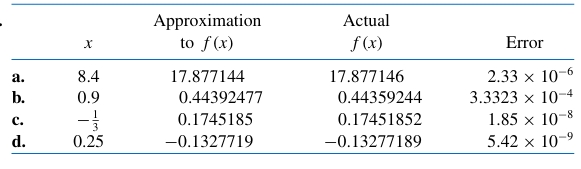
\includegraphics[width=10cm]{EndofMod3Q3sol}
\end{center}
\end{mysolution}

\item Construct the natural cubic spline for the following data.
\begin{enumerate}[label=(\alph*)]
\item
\begin{center}
\begin{tabular}{c|c}
$x$ & $f(x)$ \\
\hline
8.3 & 17.56492 \\
8.6 & 18.50515 \\
\end{tabular}
\end{center}
\item
\begin{center}
\begin{tabular}{c|c}
$x$ & $f(x)$ \\
\hline
0.8 & 0.22363362 \\
1.0 & 0.65809197 \\
\end{tabular}
\end{center}
\item
\begin{center}
\begin{tabular}{c|c}
\multicolumn{1}{c|}{$x$} & $f(x)$ \\
\hline
-0.5 & -0.0247500 \\
-0.25 & 0.3349375 \\
0 & 1.1010000 \\
\end{tabular}
\end{center}
\item
\begin{center}
\begin{tabular}{c|r}
$x$ & \multicolumn{1}{|c}{$f(x)$} \\
\hline
0.1 & -0.62049958 \\
0.2 & -0.28398668 \\
0.3 & 0.00660095 \\
0.4 & 0.24842440 \\
\end{tabular}
\end{center}
\end{enumerate}
\begin{mysolution}
The equations of the respective free cubic splines are
\[S(x)=S_i(x)=a_i+b_i(x-x_i)+c_i(x-x_i)^2+d_i(x-x_i)^3,\]
for $x$ in $[x_i, x_{i+1}]$, where the coefficients are given in the following tables.
\begin{enumerate}[label=(\alph*)]
\item ~
\begin{center}
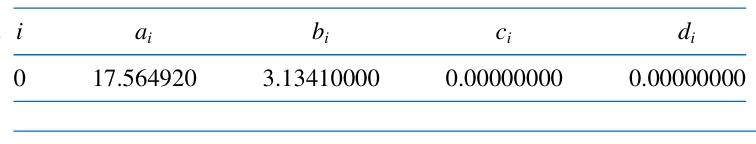
\includegraphics[width=10cm]{EndofMod3Q4sola}
\end{center}
\item ~
\begin{center}
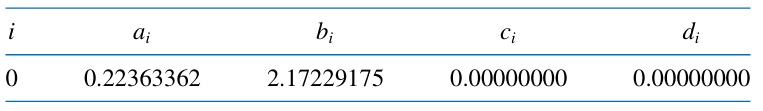
\includegraphics[width=10cm]{EndofMod3Q4solb}
\end{center}
\item ~
\begin{center}
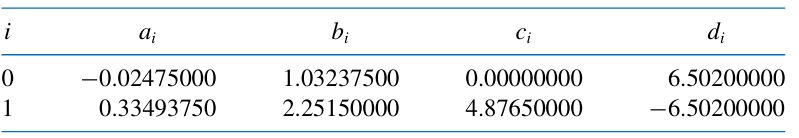
\includegraphics[width=10cm]{EndofMod3Q4solc}
\end{center}
\item ~
\begin{center}
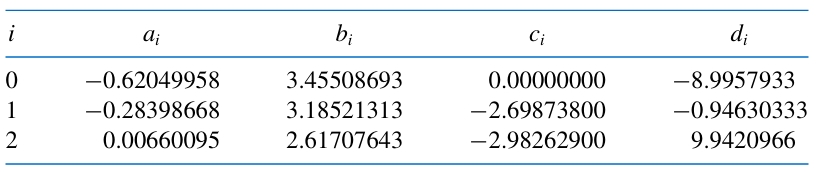
\includegraphics[width=10cm]{EndofMod3Q4sold}
\end{center}
\end{enumerate}
\end{mysolution}
\end{posttest}
%share your understanding of properties of functions and their applications to solving rates of change problems in physical phenomenon 


%\end{actsoln}

\takehome

\comy{You are now at the last part of this module. Your  task is to do a self-reflection on your learning experience.}



\references
\begin{refenumerate}
\item Kong, Q., Siauw, T., Bayen, A., (2020). Python Programming and Numerical Methods. First Edition, Academic Press,  ISBN-13 ‏ : ‎ 978-0128195499 \\
%chapter 1 pg 7-36 functions\\
%chapter 1 pg 51-83 limits and continuity\\
%chapter 1 pg 45-50 rates of change\\
%chapter 2 pg 108-120 the derivative\\
%\item Mendelson, E. (2022). Schaum's Outline of Calculus. McGraw-Hill Education.
%chapter 6 51-55 functions
%chapter 7 59-65 limits
%chapter 8 69-74 continuity
%chapter 9 77-81 derivative
%\item Calculus \mylink{https://math.libretexts.org/Bookshelves/Calculus}
%\item Chris McMullen, 2021, Essential Calculus Skills Practice Workbook with Full Solutions, Zishka Publishing, ISBN 978-1-941691-24-3
%\item R. Adams and C. Essex, 2021, Calculus: A complete Course, Addison Wesley, ISBN 13: 978-0135732588
%\item P. Abbott and H. Neill, 2018, Calculus: A Complete Introduction: The Easy Way to Learn Calculus (Teach Yourself), ISBN 13: 978-1473678446
\end{refenumerate}





%\wrapup
%To wrap-up, answer the following questions:
%
%\begin{enumerate}
%\item 
%%when do we say that a limit of a function exists?
%%\item how do we remove discontinuity in functions?
%%\item what is the relationship between the gradient of the tangent line and the derivative?
%\end{enumerate}
















%\newpage

%\facilitation


%
\begin{center}
    {\Large \textbf{FUNCTIONS OF SEVERAL VARIABLES}}\\[2mm]
(DEFINITION, DOMAIN, RANGE, GRAPHS AND LEVEL CURVES) \\[4mm]

\mycenterbox{5 minute review}%\\[4mm]
Recap the definition of a function of several variables, and the meaning of domain, range, graph and level curves of functions of several variables.
\end{center}
\mycenterbox{Warm-up.}%\\[4mm]
\problemAnswer{
Match the function with its graph (labeled I–VI).Give reasons for your choices
\begin{multicols}{3}
\begin{enumerate}[label=(\alph*)]
\item $f(x,y)=|x|+|y|$\\[4mm]
\item $f(x,y)=|xy|$
\item $f(x,y)=\frac{1}{1+x^2+y^2}$\\2mm]
\item $f(x,y)=(x^2-y^2)^2$
\item $f(x,y)=(x-y)^2$\\[4mm]
\item $f(x,y)=\sin(|x|+|y|)$
\end{enumerate}
\end{multicols}

\begin{center}
%\centering
\includegraphics[width=10cm]{MCTutorial1Q1.JPEG}
\end{center}
%\tcbox[tcbox raise base]{Warm-up}
 
%\begin{flushright}
%\begin{tikzpicture}
%    % A body
%
%
%    % Non-rectangle shapes must be drawn as polygone
%    \begin{scope}[shift={(3,0)}]
%        \draw  (0,0.5) -- (0,4) -- (.5,4) -- (.5,4.5) -- (1.,4.5) -- (4.,4.5) --(4.,4)-- (4.5,4) --(4.5,0.5) --(4.0,0.5)--(4.0,0.0)-- (.5,0) --(0.5,0.5) -- cycle;
%        % Draw symmetry lines
%        \draw [symmetry] (.5, 0.5) -- (.5,4.0);
%        \draw [symmetry] (4, 0.5) -- (4,4.0);
%        \draw [symmetry] (.5,4.0) -- (4,4.0);
%         \draw [symmetry] (.5, 0.5) -- (4, 0.5);
%        % Dimensions
%        \draw (4.5,0) -- ++(0.5,0) coordinate (D1) -- +(5pt,0);
%        \draw (4.5,4.5) -- ++(0.5,0) coordinate (D2) -- +(5pt,0);
%        \draw [dimen] (D1) -- (D2) node {6cm};
%       
%        
%        \draw (0.0,5) -- ++(0,0.5) coordinate (D1) -- +(0,+5pt);
%        \draw (0.5,5) -- ++(0,0.5) coordinate (D2) -- +(0,+5pt);
%        \draw [dimen,-] (D1) -- (D2) node [above=5pt] {$x$ cm};
%        \draw [dimen,<-] (D1) -- ++(-5pt,0);
%        \draw [dimen,<-] (D2) -- ++(+5pt,0);
%    \end{scope}
%\end{tikzpicture}
%\end{flushright}

}


\mycenterbox{Problems.}%

%\begin{center}
%\tcbox[tcbox raise base]{ Problems. Choose from the below}
%\end{center}
\problem{Exploring functions}%
\begin{enumerate}[(a)]
\item Are the following functions even, odd, or neither? What can you say
about their range?
\begin{multicols}{4}
 \begin{enumerate}[(i)]
\item $\displaystyle \frac{3x}{x^2+2}$
\item $\displaystyle \cos x+3$
\item $\displaystyle \frac{2x^3}{\cos x+3}$
\item $\displaystyle \frac{3x^4+2x^2}{\sin x+4}$
\end{enumerate}
\end{multicols}
\item Consider the functions $\sin^n x$ and $\cos^n x$, where $n$ is a positive integer.
Which are odd, which are even, and what are their periodicities?
\item What is the periodicity of $f(x) = 2 \cos x+\sin 2x$? Is it even/odd/neither?

\end{enumerate}

\problem{Cubic functions} 
Show that $x-1$ is a factor of the cubic function%
$$P(x)=x^3-2x^2-5x+6,$$
and  find the quadratic factor $Q(x)$ such that $P(x) = (x -1)Q(x)$. Factorise
$Q(x)$ and hence sketch $P(x).$

%\newpage
\problem{Sigmoid functions*.}%
For positive integers $n$, consider the family of functions
$$\displaystyle f_n= \frac{x^n}{2^n+x^n}.$$
\begin{enumerate}[(a)]
\item What are appropriate domains and ranges for $f_n(x)$? Do they depend on $n$?

\item Is $f_n(x)$ even, odd, or neither? Does this depend on $n$?

\item Show that for $x\geq 0$, $f_n(x)$ are strictly increasing functions and that
$0\leq f_n(x) < 1.$
\item What is the value of $f_n(2)$? Does it depend on $n$?

\item By considering the values of $f_n(1.9)$ and $f_n(2.1)$ for $n = 2, 4, 8, 16, 32$ and
$64$, show that the graph of $f_n(x)$ for $x\ge 0$ is an increasing sigmoid (that
is, $S$-shaped) function that approaches a step function as $n\rightarrow \infty$.
\end{enumerate}

\mycenterbox{Selected answers and hints}%

For the warm-up, $V(x)=4x(3-x)^2$. Writing $x=1+\epsilon$, we get
$$V = 4(1 +\epsilon)(3- (1+\epsilon))^2=4(4-\epsilon^2(3-\epsilon)).$$
If $-1<\epsilon<2$ then $\epsilon^2 (3-\epsilon)\ge 0$, with equality when $\epsilon=0$. Thus the maximum
value of $V$ occurs when $\epsilon= 0$, i.e. $x = 1\rm{cm}$.

\begin{enumerate}
\item 
\begin{enumerate}[(i)]
\item Odd. The range is the interval  $[-\frac{3}{4}\sqrt{2},\; \frac{3}{4}\sqrt{2}]$
\item Even. The range is the interval $[2, 4]$.
\item Odd. The range is all of $\mathbb R$.
\item Neither. (For example, writing $\displaystyle \frac{5}{\sin x+4}$ we have $\displaystyle f(1)= \frac{5}{\sin (1)+4} \equiv 1.032 (3\rm{dp})$ which is neither $f(1)$ nor $-f(1)$.)\\[4mm]
The range is the nonnegative reals $[0,\infty)$

\end{enumerate}
\end{enumerate}











%
%\newpage
%
%\newpage
%
%
%\newtheorem{definition}[subsection]{Definition}
%\newtheorem{example}[subsection]{Example}
\newtheorem{cor}[subsection]{Corollary}
\newtheorem{pro}[subsection]{Proposition}
\newtheorem{theo}[subsection]{Theorem}
\newtheorem{lem}[subsection]{Lemma}
%\newtheorem{rem}[subsection]{Remark}

\definecolor{main}{HTML}{5989cf}    % setting main color to be used
\definecolor{sub}{HTML}{cde4ff}     % setting sub color to be used

\tcbset{
    sharp corners,
    colback = white,
    before skip = 0.2cm,    % add extra space before the box
    after skip = 0.5cm      % add extra space after the box
}                           % setting global options for tcolorbox

% You can copy any following box you like to your code.
\newtcolorbox{boxA}{
    fontupper = \bf,
    boxrule = 1.5pt,
    colframe = black % frame color
}

\newtcolorbox{boxB}{
    fontupper = \bf\color{main}, % font color
    boxrule = 1.5pt,
    colframe = main,
    rounded corners,
    arc = 5pt   % corners roundness
}
\newtcolorbox{boxC}{
    colback = sub, % background color
    boxrule = 0pt  % no borders
}

\newtcolorbox{boxD}{
    colback = sub, 
    colframe = main, 
    boxrule = 0pt, 
    toprule = 3pt, % top rule weight
    bottomrule = 3pt % bottom rule weight
}

\hypersetup{
    colorlinks=true,
    linkcolor=blue,
    filecolor=magenta,      
    urlcolor=cyan,
    pdftitle={Overleaf Example},
    pdfpagemode=FullScreen,
    }

\urlstyle{same}


\coursetitle{\mtthreeiii}{MT303}
\developers{Wyclife Rao}
\reviewers{Dr Irene Sitawa}
\modulenumber{4}
\modulename{Numerical Diferentiation and Integration}

% courses
\thispagestyle{empty}
\begin{tikzpicture}[overlay,remember picture,font=\sffamily\bfseries]
 \draw[ultra thick,c4,name path=big arc] ([xshift=-2mm]current page.north) arc(150:285:11) coordinate[pos=0.225] (x0);
 \begin{scope}
  \clip ([xshift=-2mm]current page.north) arc(150:285:11) --(current page.north east);
  \fill[c4!50,opacity=0.25] ([xshift=4.55cm]x0) circle (4.55);
  \fill[c4!50,opacity=0.25] ([xshift=3.4cm]x0) circle (3.4);
  \fill[c4!50,opacity=0.25] ([xshift=2.25cm]x0) circle (2.25);
  \draw[ultra thick,c4!50] (x0) arc(-90:30:6.5);
  \draw[ultra thick,c4] (x0) arc(90:-30:8.75);
  \draw[ultra thick,c4!50,name path=arc1] (x0) arc(90:-90:4.675);
  \draw[ultra thick,c4!50] (x0) arc(90:-90:2.875);
  \path[name intersections={of=big arc and arc1,by=x1}];
  \draw[ultra thick,c4,name path=arc2] (x1) arc(135:-20:4.75);
  \draw[ultra thick,c4!50] (x1) arc(135:-20:8.75);
  \path[name intersections={of=big arc and arc2,by={aux,x2}}];
  \draw[ultra thick,c4!50] (x2) arc(180:50:2.25);
 \end{scope} 
 \path[decoration={text along path,text color=c4,
                 raise = -2.8ex,
                 text  along path,
                 text = {},%|\sffamily\bfseries|02/18/2019
                 text align = center,
             },
             decorate
         ] ([xshift=-2mm]current page.north) arc(150:245:11);
 %
 \newcommand\add{4cm}
 \begin{scope}%[shift={(5,0)}]
  \path[clip,postaction={fill=c3}]
  ([xshift=2cm+\add,yshift=-8cm]current page.center) rectangle ++ (4.6,7.7);
  \draw[c5,ultra thick,fill=c2] ([xshift=0.5cm+\add,yshift=-8cm]current page.center)
   ([xshift=0.5cm+\add,yshift=-8cm]current page.center)  arc(180:60:2)
    |- ++ (-3,6) --cycle;
  \draw[ultra thick,c5] ([xshift=-1.5cm+\add,yshift=-8cm]current page.center) 
  arc(180:0:2);
  \draw[ultra thick,c5] ([xshift=0.5cm+\add,yshift=-8cm]current page.center) 
  arc(180:0:2);
  \draw[ultra thick,c5] ([xshift=2.5cm+\add,yshift=-8cm]current page.center) 
  arc(180:0:2);
  \draw[ultra thick,c5] ([xshift=4.5cm+\add,yshift=-8cm]current page.center) 
  arc(180:0:2);
  \fill[white] ([xshift=2.5cm+\add,yshift=-8cm]current page.center) +(60:2) circle(1.5mm)
  node[above
  right=0mm,text=c5!80!black]{$\rho:=\dfrac{1+\sqrt{-3}}{2}$};
 \end{scope}
 %
 \fill[c1] ([xshift=2cm+\add,yshift=-8cm]current page.center) rectangle ++ (-30.7,7.7);
 \node[text=white,anchor=west,scale=2.3,inner sep=0pt] at
 ([xshift=-10cm,yshift=-1.8cm]current page.center) {\color{ulabgold} LEARNING};
 \node[text=white,anchor=west,scale=5,inner sep=0pt] at
 ([xshift=-10cm,yshift=-3.25cm]current page.center) {MODULE \dpmdnumber};
 \node[text=white,anchor=west,scale=2.5,inner sep=0pt,text width=.4\textwidth] at
 ([xshift=-10cm,yshift=-6cm]current page.center) {\dpmdname};
 \node[text=white,anchor=east,scale=2,inner sep=0pt] at
 ([xshift=5.7cm,yshift=-7.5cm]current page.center) {\color{ulabgold}The Open University of Kenya};
 %
% \draw[gray,line width=5mm] 
% ([xshift=2mm,yshift=-1mm]current page.south west) rectangle ([xshift=-2mm,yshift=1mm]current
% page.north east);
\end{tikzpicture}

%\newpage
\pagenumbering{roman}
\thispagestyle{empty}%firstpage


\begin{center}
\vspace*{2cm}
{\Huge\bf BACHELOR OF TECHNOLOGY EDUCATION}\\[3cm]  


%{\fontsize{80}{40}\selectfont \dpcoursecode}\\[2cm]
%
%{\fontsize{30}{40} \selectfont \dpcoursename}\\[2cm]

%\rule{\textwidth}{1pt}
%\vspace{2cm}

%{\fontsize{40}{40}\selectfont \bf Module~\dpmdnumber}\\[2cm]
%
%{\fontsize{30}{40}\selectfont \bf \dpmdname}\\

\vfill
\begin{flushright}
\begin{minipage}{.6\textwidth}
\begin{tcolorbox}%[text ]
\begin{tabular}{ll}%\hline
\subtitle{Developed by:}&\displaydevelopers\\
&\\
\subtitle{Reviewed by:}&\makecell[l]{\displayreviewers}\\
\end{tabular}
\end{tcolorbox}
\end{minipage}\hspace*{-3.5cm}
\end{flushright}
\vspace*{-2.5cm}
\end{center}

\newpage
\thispagestyle{empty}
\null
\vfill
{\renewcommand\arraystretch{1.5}
\begin{tabular}{|l|l|}\hline
\subtitle{Programme Title} & Bachelor of Technology Education \\\hline
\subtitle{Course Title} & \fullcoursename\\\hline
\subtitle{Learning Module number} & Module \dpmdnumber\\\hline
\subtitle{Learning module title} & \dpmdname \\\hline
\subtitle{Module Developer} & \displaydevelopers\\\hline
\subtitle{Reviewed by} & \displayreviewers\\\hline
%\subtitle{Vision} & \vision\\\hline
%\subtitle{Audience description} & \\\hline
\end{tabular}}
\clearpage

%\section{COURSE LEARNING GUIDE}


\subsection*{Preparing for Online and Distance Learning}

This course offers you the opportunity to enter an online space where you can engage with fellow students at the university. The online forums, exercises, tasks and materials have been designed by the course facilitators in such a way that you can draw directly from their knowledge and share in their scholarly interest in online learning and assessment

We hope you will use your access to this virtual classroom to raise all your questions on the course module, to build a network great learners and to share your own thoughts and experiences to the benefit of your fellow students.

   
There are a number of steps you can take to ensure you are well prepared to make the most of this learning opportunity. This resource should prompt you to consider the following:


 \begin{enumerate}[label=\cb$\square$]
   \item How can you best prepare the space where you expect you will spend most of your time engaging in online learning (i.e. in your home or office, or even during your commute to work or whilst traveling)?
  \item   What can you do to ensure you keep working through the course material, even when you do not have Internet access?
    \item How can you familiarise yourself with the course layout, in order to be able to navigate through the steps with ease?
    \item What are the communication strategies and best practices you could consider to best engage with your fellow students and the course facilitators?
    \item What do you do when you need academic or technical support?

 \end{enumerate} 

\subsection*{General Module Guide}

The authors of this module believe that imparting knowledge should always be a mutual relationship between the students and the teachers. Students can actively construct knowledge through experiences gained in reading and answering the learning modules.

You should take time to read everything written in the module, actively and religiously solve all the exercises included to finish this course and be able to gain all the competencies and skills expected to demonstrate the learning outcomes as stated in this course. If you finish with full confidence that you understand and can apply all the knowledge you gain in this course, then you are sure to succeed in tackling the next higher subjects in your chosen course.

In this course, you will be taught not only the knowledge you need to demonstrate your learning outcomes, but you will also gain discipline, perseverance, higher thinking skills, and resourcefulness that would help strengthen your foundation to succeed in life. To successfully finish the course, you must follow the guides set forth in using this module.


\begin{description}[{format=\textcolor{ulabblue}}]
\item[STUDY ENVIRONMENT.]\leavevmode\\
Before engaging into the module, make sure that you are comfortable enough and diminish distractions. Make sure that you develop a study routine to perform and accomplish all the activities set forth by the module.
%\newpage

\item[MODE OF DELIVERY.]\leavevmode\\
Students are required to get a access a digitised copy of the module from the Virtue Learning Environment. As an open and distance learner, you should be able to learn independently and optimise the learning modes and environment available to you as much of  the delivery of all the lessons will be done asynchronously. Your success will greatly depend on your self-motivation and discipline to get your work done without your instructor to remind you from time to time.

\item[STUDY SCHEDULE.] \leavevmode\\
Remember that you have other subjects to attend to, hence, you must manage your time so that you will not be left behind in any of them. Create your own learning plan for each course to make sure that you can perform all the activities. Do not procrastinate your work, remember that time wasted can never be retrieved back. Make sure that even if you are at home, you are a student enrolled in a program, where the learning of all its courses greatly depends on your will to learn as the materials you need are all in your hands. So always be aware of your daily tasks.

\item[PRACTICE EXERCISE.]\leavevmode\\
To measure your learning from your reading, you are given practice exercises which you are supposed to answer daily. This will prepare you in performing your main task.

\item[ONLINE GROUP CHAT.]\leavevmode\\
I am going to create an online Discussion Forum and QA Forum  on the VLE.  This will serve as a room for discussion on the topics and activities found in your module.

\item[RECOMMENDED REFERENCES FOR SUPPLEMENTARY READING.]\leavevmode\\
You are given links that you need to access online. These links are online references such as e-books, online activities, and tutorial videos of the topic. These are other references you can use to further understand the topic and gain additional knowledge and skills.

\item[MAIN TASK.]\leavevmode\\
You are given a task that will require you to apply the knowledge and skills you learned from the module. This can be a group or individual activity which will measure your higher order thinking skills you acquired throughout the topic.

\item[RUBRICS. ]\leavevmode\\
This is a tool to guide you in performing your main task. Through this, you will be able to know the specific indicators that should be found in your task. This is to assess your constructive behaviour towards your learning application. You will be rated according to a 4-point scale shown below.
\begin{center}
{\color{ulabgold} \bf 4 − Excellent\quad\quad   3 −Good\quad\quad    2 − Fair \quad\quad  1 −Poor}
\end{center}
\item[REFLECTIONS.]\leavevmode\\
Writing your reflection will be a passageway to express your experiential learning in using this module. In your honest recall, write everything that you think happened to you during your learning experience in this module. Use the guide questions below:
\begin{description}[{format=\textcolor{ulabblue}}]
\item[First paragraph. ]\leavevmode\\
How was your learning experience? Maybe you can consider describing the effect of the parts of the module (sequence, discussions, examples, practice exercises, online activities, and the main task) in your learning experience. You can point out the strength and weakness of each part so that we can consider it for future improvement of this instructional material.
\item[Second paragraph.  ]\leavevmode\\
What did you learn? Did you successfully acquire the learning outcomes?

\item[Third paragraph.]\leavevmode\\
How can you use what you learned in the future?
\end{description}
\end{description}

\section{ASSESSMENT  TASKS \& EXAMINATION   RULES AND GUIDELINES}

\begin{enumerate}[label=\cb\arabic*.]
\item {\cb SUBMISSION OF ASSESSMENT TASTS.}

Since mathematical skills are best acquired through constant practice, you are encouraged to answer at least two (2) exercises a day. These practice exercises will not be graded but it will help you develop your thinking skills which will prepare you in the performance of your main tasks. You are required to submit your practice exercises every week.
\begin{center} {\cg Usually submission deadlines are set on Saturday 11:59PM EAT} \end{center}

\item  {\cb GROUP CHAT.}

You can post questions, solutions, and comment to other's post. Please be reminded that our group chat is exclusive only for discussion on topics related to this course. Everyone is required to actively participate in the discussions. Also, trolling is highly discouraged. Always observe proper online etiquettes when participating in discussions.
\begin{center} {\cb RULE OF THUMB: ALWAYS THINK BEFORE YOU CLICK} \end{center}

\item  {\cb MAIN TASK. }

Complete documentation during the preparation of your task is required to ensure that every member of the group participated and contributed in the task. May it be photos or screenshots of your virtual meetings or group works. You are going to submit it as attachment of your main task the same way as the practice exercises.



\item {\cb RECOMMENDED REFERENCES FOR SUPPLEMENTARY READING.} 

You can explore online for other references that is related to the topic to gain additional information about the topic. Do not share or post inappropriate materials online or even privately.
\end{enumerate}

\subsection*{Requirements to pass the course}

Compiled Continuous  Assignment/Activities and Tasks  with Final Performance Examination.

\subtitle{Grading System}
\begin{center}
{\renewcommand\arraystretch{1.5}
\begin{tabular}{|l|c|}\hline
Continuous Activities and Tasks  &  50\%\\\hline
Final Performance Examination. &  50\%\\\hline
\end{tabular}
}
\end{center}
%\newpage










%\subsection{INTRODUCTORY MESSAGE}

%A warm welcome to \;  \fullcoursename, {\bf Module on \dpmdname}.



%By this module learning resource, we aim to enable you  achieve the relevant competencies, depict skill, action and purpose successfully. 
 

%It has been designed to provide you with fun and meaningful opportunities for guided and independent learning at your own pace and time. You will be enabled to process the contents of the learning material while being an active learner. Your academic success lies in your own hands.  This module has the following parts and corresponding icons:





{
\renewcommand\arraystretch{4}
\begin{longtblr}{
width=\linewidth,
 colspec={ Q[1,c,f] Q[1.5,r,m] Q[4,l,m] },
%row{1} = { font=\bfseries },
% rowhead = 1,
  caption={ }, 
  label={ },
  rowsep = 4pt,
  hlines = {ulabblue!20, 1pt},
  vlines = {ulabblue!20, 1pt},
}

\includegraphics[width=2cm]{img/audience} & {\bf AUDIENCE}  &  This is a description of a target audience.   \\
{\fontsize{40}{30}\selectfont\color{ulabblue}\faCogs}& {\bf MODULE DESCRIPTION} & 
This part explains the importance of the topics discussed in the module. It will also give you a sneak peek of what you will learn and what is expected from you at the end of the module.\\

\includegraphics[width=2cm]{img/target.png} &  {\bf  EXPECTATION} & These are what you will be able to know after completing the lessons in the module\\

\includegraphics[width=2cm]{img/preactivities} & {\bf PRE-ACTIVITY} &
This activity is to get you set, activate and engage schema to learn the module. Through this activity, you will know the relevance of this activity to the topic that will be discussed in the module.\\

\includegraphics[width=2cm]{img/pretest} &  {\bf PRE - ASSESSMENT} & This will measure your prior knowledge and the concepts to be mastered throughout the lesson. \\

\includegraphics[width=1.7cm]{img/rewind} &  {\bf  RECAP} & This section will measure what learnings and skills that you understand from the previous lesson.\\

\includegraphics[width=1.5cm]{img/lesson} &  {\bf  LESSON} & This section will discuss the topic for this module.\\

\includegraphics[width=2cm]{img/activities} &  {\bf  ACTIVITIES} & This is a set of activities you will perform.\\

\includegraphics[width=2cm]{img/summary} &  {\bf  WRAP UP} & This section summarizes the concepts and applications of the lessons.\\

\includegraphics[width=2cm]{img/discussion}& {\bf DISCUSSIONS} &
This is the meat of the module. The discussion is aligned to the topic learning outcomes that is expected of you to acquire at the end of the module.\\

\includegraphics[width=1.8cm]{img/value} &  {\bf  VALUING} & This part will check the integration of values in the learning competency you will take home.\\

\includegraphics[width=1.8cm]{img/posttest} &  {\bf  POST - ASSESSMENT} & This will measure how much you have learned from the entire module.\\

\includegraphics[width=1.8cm]{img/selfreflect} & {\bf REFLECTION }
&
This part is for you to share your thoughts by writing your reflection, make sure to check your grammar and spelling to ensure the readability and so that it will not alter the thought being delivered. 
\end{longtblr}
}









%\vfill

\audience
\begin{oldactivity}{Audience Description}{
\includegraphics[width=22mm]{img/audience}}{}
This module is offered to all students taking the Bachelor of Technology Education. As an open and distance learner, you should be able to learn independently and optimise the learning modes and environment available to you. Before you begin this course, please confirm the course material, the course requirements and how the course is conducted.
\end{oldactivity}
%\newpage
\pagenumbering{arabic}



\mddescription
This module guides you into a detailed discussion of the concepts of parametric curves and numerical differentiation and integration. Specificcally you will learn about
\begin{itemize}
\item parametric curves
\item numerical differentiation
\item Richardson's extrapolation
\item elements of numerical integration 
\end{itemize}
%\expectations
%\begin{objenumerate}
%
%\end{objenumerate}

\begin{mlos}
\item Define parametric curves and numerical differentiation concepts.
\item Explain Richardson’s extrapolation and its role in improving derivative estimates.
\item Perform numerical differentiation on parametric curves using finite difference methods.
\item Evaluate the accuracy of numerical integration techniques applied to parametric functions. 
\end{mlos}

\section{Parametric Curves}
\videolesson
\begin{selfvideo}[1]
%LESSON 3: 
This video presents a discussion on parametric curves in polynomial approximation. Follow the discussion and then solve the problems in the subsequent quiz.
\end{selfvideo}
%\begin{boxB}Question: \end{boxB}
In this section we will see how to represent general curves by using a parameter to express both the $x$ - and $y$-coordinate variables. 
%Any good book\\[0pt]
%on computer graphics will show how this technique can be extended to represent general curves and surfaces in space. (See, for example, [FVFH].)
%

\begin{figure}[h]
\centering
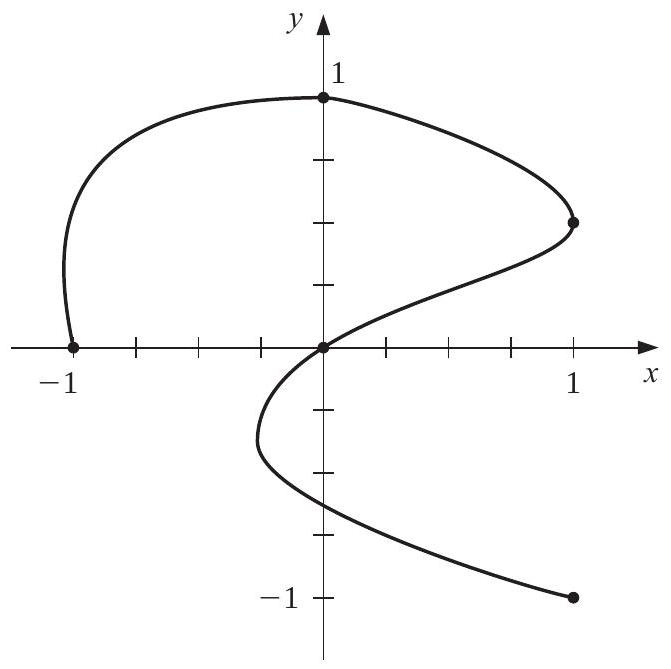
\includegraphics[width=6cm]{2025_05_15_4109a88b43049bd640d1g-61.JPG}
\caption{\scriptsize Figure 1}
\label{fig:2025_05_15_4109a88b43049bd640d1g-61}
\end{figure}

A straightforward parametric technique for determining a polynomial or piecewise polynomial to connect the points $\left(x_{0}, y_{0}\right),\left(x_{1}, y_{1}\right), \ldots,\left(x_{n}, y_{n}\right)$ in the order given is to use a parameter $t$ on an interval $\left[t_{0}, t_{n}\right]$, with $t_{0}<t_{1}<\cdots<t_{n}$, and construct approximation functions with

$$
x_{i}=x\left(t_{i}\right) \quad \text { and } \quad y_{i}=y\left(t_{i}\right), \quad \text { for each } i=0,1, \ldots, n .
$$

The following example demonstrates the technique in the case where both approximating functions are Lagrange interpolating polynomials.

\begin{example}
Construct a pair of Lagrange polynomials to approximate the curve shown in Figure \ref{fig:2025_05_15_4109a88b43049bd640d1g-61}, using the data points shown on the curve.
\end{example}

\begin{mysolution}
There is flexibility in choosing the parameter, and we will choose the points $\left\{t_{i}\right\}_{i=0}^{4}$ equally spaced in $[0,1]$, which gives the data in Table below
\begin{center}
\begin{tabular}{lrlllr}
\hline
$i$ & 0 & 1 & 2 & \multicolumn{1}{c}{3} & 4 \\
\hline
$t_{i}$ & 0 & 0.25 & 0.5 & 0.75 & 1 \\
$x_{i}$ & -1 & 0 & 1 & 0 & 1 \\
$y_{i}$ & 0 & 1 & 0.5 & 0 & -1 \\
\hline
\end{tabular}
\end{center}
This produces the interpolating polynomials
\[x(t)=\left(\left(\left(64 t-\frac{352}{3}\right) t+60\right) t-\frac{14}{3}\right) t-1\]
and
\[y(t)=\left(\left(\left(-\frac{64}{3} t+48\right) t-\frac{116}{3}\right) t+11\right) t.\]
Plotting this parametric system produces the graph shown in blue in Figure \ref{fig:2025_05_15_4109a88b43049bd640d1g-62}. Although it passes through the required points and has the same basic shape, it is quite a crude approximation to the original curve. A more accurate approximation would require additional nodes, with the accompanying increase in computation.
\end{mysolution}

\begin{figure}[h]
\centering
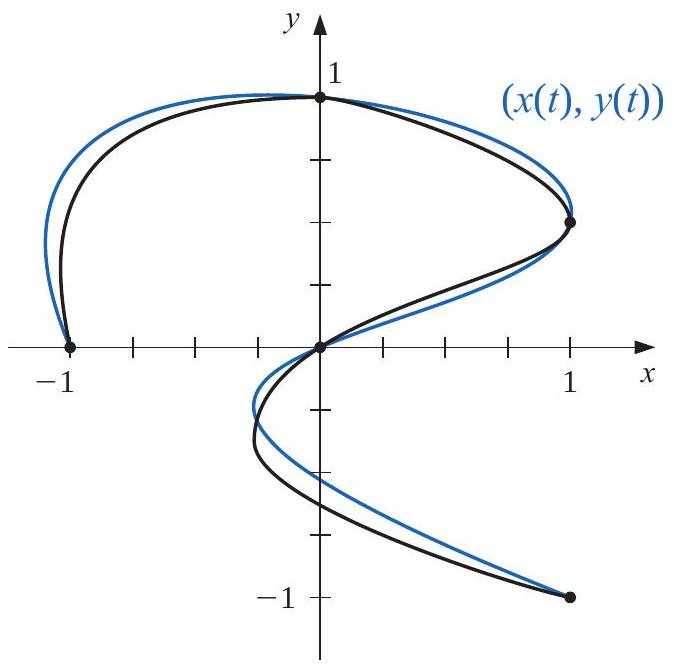
\includegraphics[width=6cm]{2025_05_15_4109a88b43049bd640d1g-62.JPG}
\caption{\scriptsize Figure 2}
\label{fig:2025_05_15_4109a88b43049bd640d1g-62}
\end{figure}


%Figure 3.16
%
%A successful computer design system needs to be based on a formal mathematical theory so that the results are predictable, but this theory should be performed in the background so that the artist can base the design on aesthetics.\\
%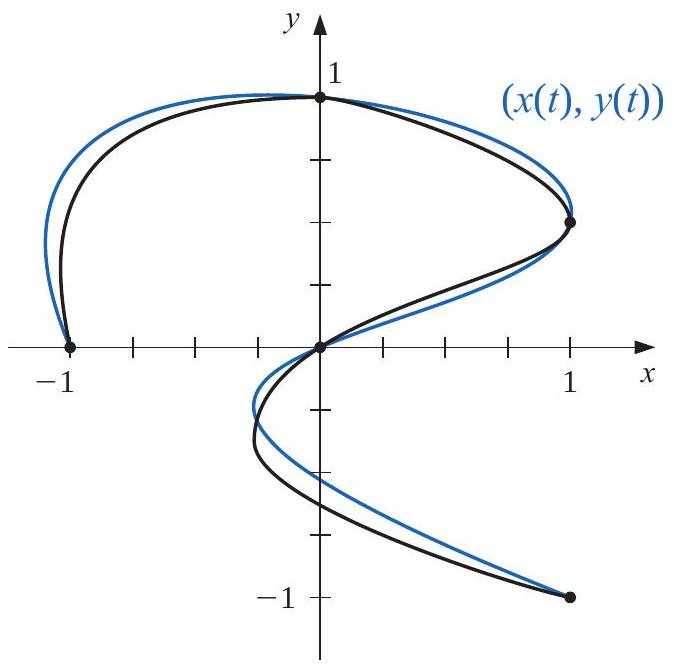
\includegraphics[max width=\textwidth, center]{2025_05_15_4109a88b43049bd640d1g-62}
%
%Parametric Hermite and spline curves can be generated in a similar manner, but these also require extensive computational effort.

%Applications in computer graphics require the rapid generation of smooth curves that can be easily and quickly modified. For both aesthetic and computational reasons, changing one portion of these curves should have little or no effect on other portions of the curves. This eliminates the use of interpolating polynomials and splines since changing one portion of these curves affects the whole curve.
%
The choice of curve for use in computer graphics is generally a form of the piecewise cubic Hermite polynomial. Each portion of a cubic Hermite polynomial is completely determined by specifying its endpoints and the derivatives at these endpoints. As a consequence, one portion of the curve can be changed while leaving most of the curve the same. Only the adjacent portions need to be modified to ensure smoothness at the endpoints. The computations can be performed quickly, and the curve can be modified a section at a time.

The problem with Hermite interpolation is the need to specify the derivatives at the endpoints of each section of the curve. Suppose the curve has $n+1$ data points $\left(x\left(t_{0}\right), y\left(t_{0}\right)\right), \ldots$,\\$\left(x\left(t_{n}\right), y\left(t_{n}\right)\right)$, and we wish to parameterize the cubic to allow complex features. Then we must specify $x^{\prime}\left(t_{i}\right)$ and $y^{\prime}\left(t_{i}\right)$, for each $i=0,1, \ldots, n$. This is not as difficult as it would first appear, since each portion is generated independently. We must ensure only that the derivatives at the endpoints of each portion match those in the adjacent portion. Essentially, then, we can simplify the process to one of determining a pair of cubic Hermite polynomials in the parameter $t$, where $t_{0}=0$ and $t_{1}=1$, given the endpoint data $(x(0), y(0))$ and $(x(1), y(1))$ and the derivatives $d y / d x$ (at $t=0$ ) and $d y / d x$ (at $t=1$ ).

Notice, however, that we are specifying only six conditions, and the cubic polynomials in $x(t)$ and $y(t)$ each have four parameters, for a total of eight. This provides flexibility in choosing the pair of cubic Hermite polynomials to satisfy the conditions, because the natural form for determining $x(t)$ and $y(t)$ requires that we specify $x^{\prime}(0), x^{\prime}(1), y^{\prime}(0)$, and $y^{\prime}(1)$. The explicit Hermite curve in $x$ and $y$ requires specifying only the quotients

$$
\frac{d y}{d x}(t=0)=\frac{y^{\prime}(0)}{x^{\prime}(0)} \quad \text { and } \quad \frac{d y}{d x}(t=1)=\frac{y^{\prime}(1)}{x^{\prime}(1)} .
$$

By multiplying $x^{\prime}(0)$ and $y^{\prime}(0)$ by a common scaling factor, the tangent line to the curve at $(x(0), y(0))$ remains the same, but the shape of the curve varies. The larger the scaling\\
factor, the closer the curve comes to approximating the tangent line near $(x(0), y(0))$. A similar situation exists at the other endpoint $(x(1), y(1))$.

To further simplify the process in interactive computer graphics, the derivative at an endpoint is specified by using a second point, called a guide point, on the desired tangent line. The farther the guide point is from the node, the more closely the curve approximates the tangent line near the node.

In Figure \ref{fig:2025_05_15_4109a88b43049bd640d1g-63(1)}, the nodes occur at ( $x_{0}, y_{0}$ ) and ( $x_{1}, y_{1}$ ), the guide point for ( $x_{0}, y_{0}$ ) is \\$\left(x_{0}+\alpha_{0}, y_{0}+\beta_{0}\right)$, and the guide point for $\left(x_{1}, y_{1}\right)$ is $\left(x_{1}-\alpha_{1}, y_{1}-\beta_{1}\right)$. The cubic Hermite polynomial $x(t)$ on $[0,1]$ satisfies

$$
x(0)=x_{0}, \quad x(1)=x_{1}, \quad x^{\prime}(0)=\alpha_{0}, \quad \text { and } \quad x^{\prime}(1)=\alpha_{1} .
$$

%Figure 3.17\\
\begin{figure}
\centering
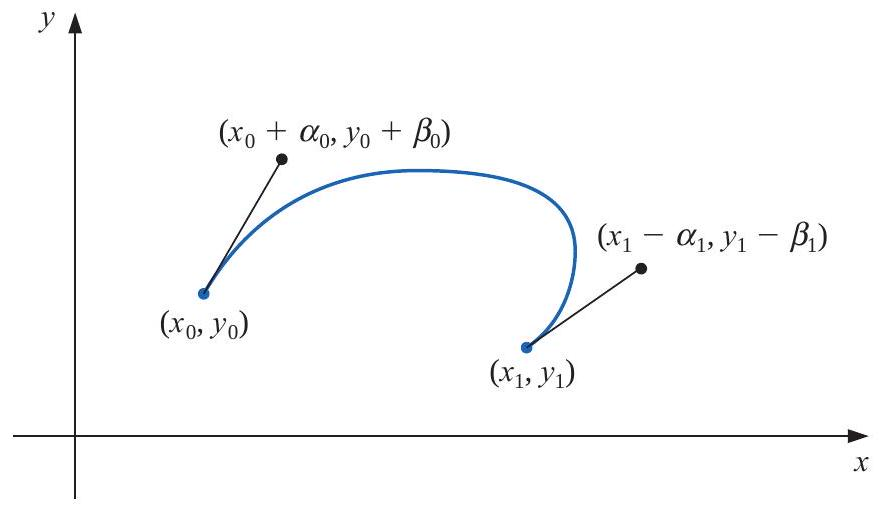
\includegraphics[width=9cm]{2025_05_15_4109a88b43049bd640d1g-63(1).JPG}
\caption{\scriptsize Figure 3 }
\label{fig:2025_05_15_4109a88b43049bd640d1g-63(1)}
\end{figure}

The unique cubic polynomial satisfying these conditions is


\begin{equation}\label{eqn:paramet1}
x(t)=\left[2\left(x_{0}-x_{1}\right)+\left(\alpha_{0}+\alpha_{1}\right)\right] t^{3}+\left[3\left(x_{1}-x_{0}\right)-\left(\alpha_{1}+2 \alpha_{0}\right)\right] t^{2}+\alpha_{0} t+x_{0}
\end{equation}


In a similar manner, the unique cubic polynomial satisfying

$$
y(0)=y_{0}, \quad y(1)=y_{1}, \quad y^{\prime}(0)=\beta_{0}, \quad \text { and } \quad y^{\prime}(1)=\beta_{1}
$$

is


\begin{equation}\label{eqn:paramet2}
y(t)=\left[2\left(y_{0}-y_{1}\right)+\left(\beta_{0}+\beta_{1}\right)\right] t^{3}+\left[3\left(y_{1}-y_{0}\right)-\left(\beta_{1}+2 \beta_{0}\right)\right] t^{2}+\beta_{0} t+y_{0}
\end{equation}


\begin{example}
Determine the graph of the parametric curve generated Eq. \ref{eqn:paramet1} and \ref{eqn:paramet2} when the end points are $\left(x_{0}, y_{0}\right)=(0,0)$ and $\left(x_{1}, y_{1}\right)=(1,0)$, and respective guide points, as shown in Figure \ref{fig:2025_05_15_4109a88b43049bd640d1g-63}
\end{example}

\begin{figure}[h]
\centering
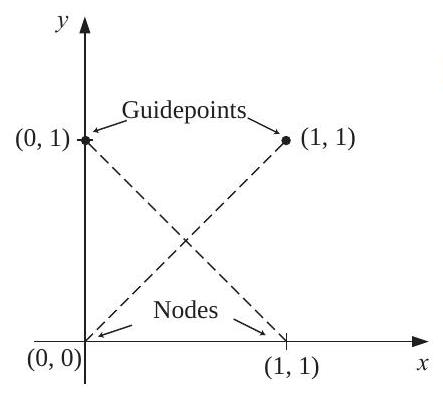
\includegraphics[width=6cm]{2025_05_15_4109a88b43049bd640d1g-63}
\caption{\scriptsize Figure $4$}
\label{fig:2025_05_15_4109a88b43049bd640d1g-63}
\end{figure}
%
%Figure 3.18 Figure 3.18 are $(1,1)$ and $(0,1)$.
%

\begin{mysolution}
The endpoint information implies that $x_{0}=0, x_{1}=1, y_{0}=0$, and $y_{1}=0$, and the guide points at $(1,1)$ and $(0,1)$ imply that $\alpha_{0}=1, \alpha_{1}=1, \beta_{0}=1$, and $\beta_{1}=-1$. Note that the slopes of the guide lines at $(0,0)$ and $(1,0)$ are, respectively

$$
\frac{\beta_{0}}{\alpha_{0}}=\frac{1}{1}=1 \quad \text { and } \quad \frac{\beta_{1}}{\alpha_{1}}=\frac{-1}{1}=-1
$$

Equations \ref{eqn:paramet1} and \ref{eqn:paramet2} imply that for $t \in[0,1]$ we have

$$
x(t)=[2(0-1)+(1+1)] t^{3}+[3(0-0)-(1+2 \cdot 1)] t^{2}+1 \cdot t+0=t
$$

and

$$
y(t)=[2(0-0)+(1+(-1))] t^{3}+[3(0-0)-(-1+2 \cdot 1)] t^{2}+1 \cdot t+0=-t^{2}+t .
$$

This graph is shown as (a) in Figure \ref{fig:2025_05_15_4109a88b43049bd640d1g-64}, together with some other possibilities of curves produced by Eqs. \ref{eqn:paramet1} and \ref{eqn:paramet2} when the nodes are $(0,0)$ and $(1,0)$ and the slopes at these nodes are $1$ and $-1$ , respectively.
\end{mysolution}

\begin{figure}[h]
\centering
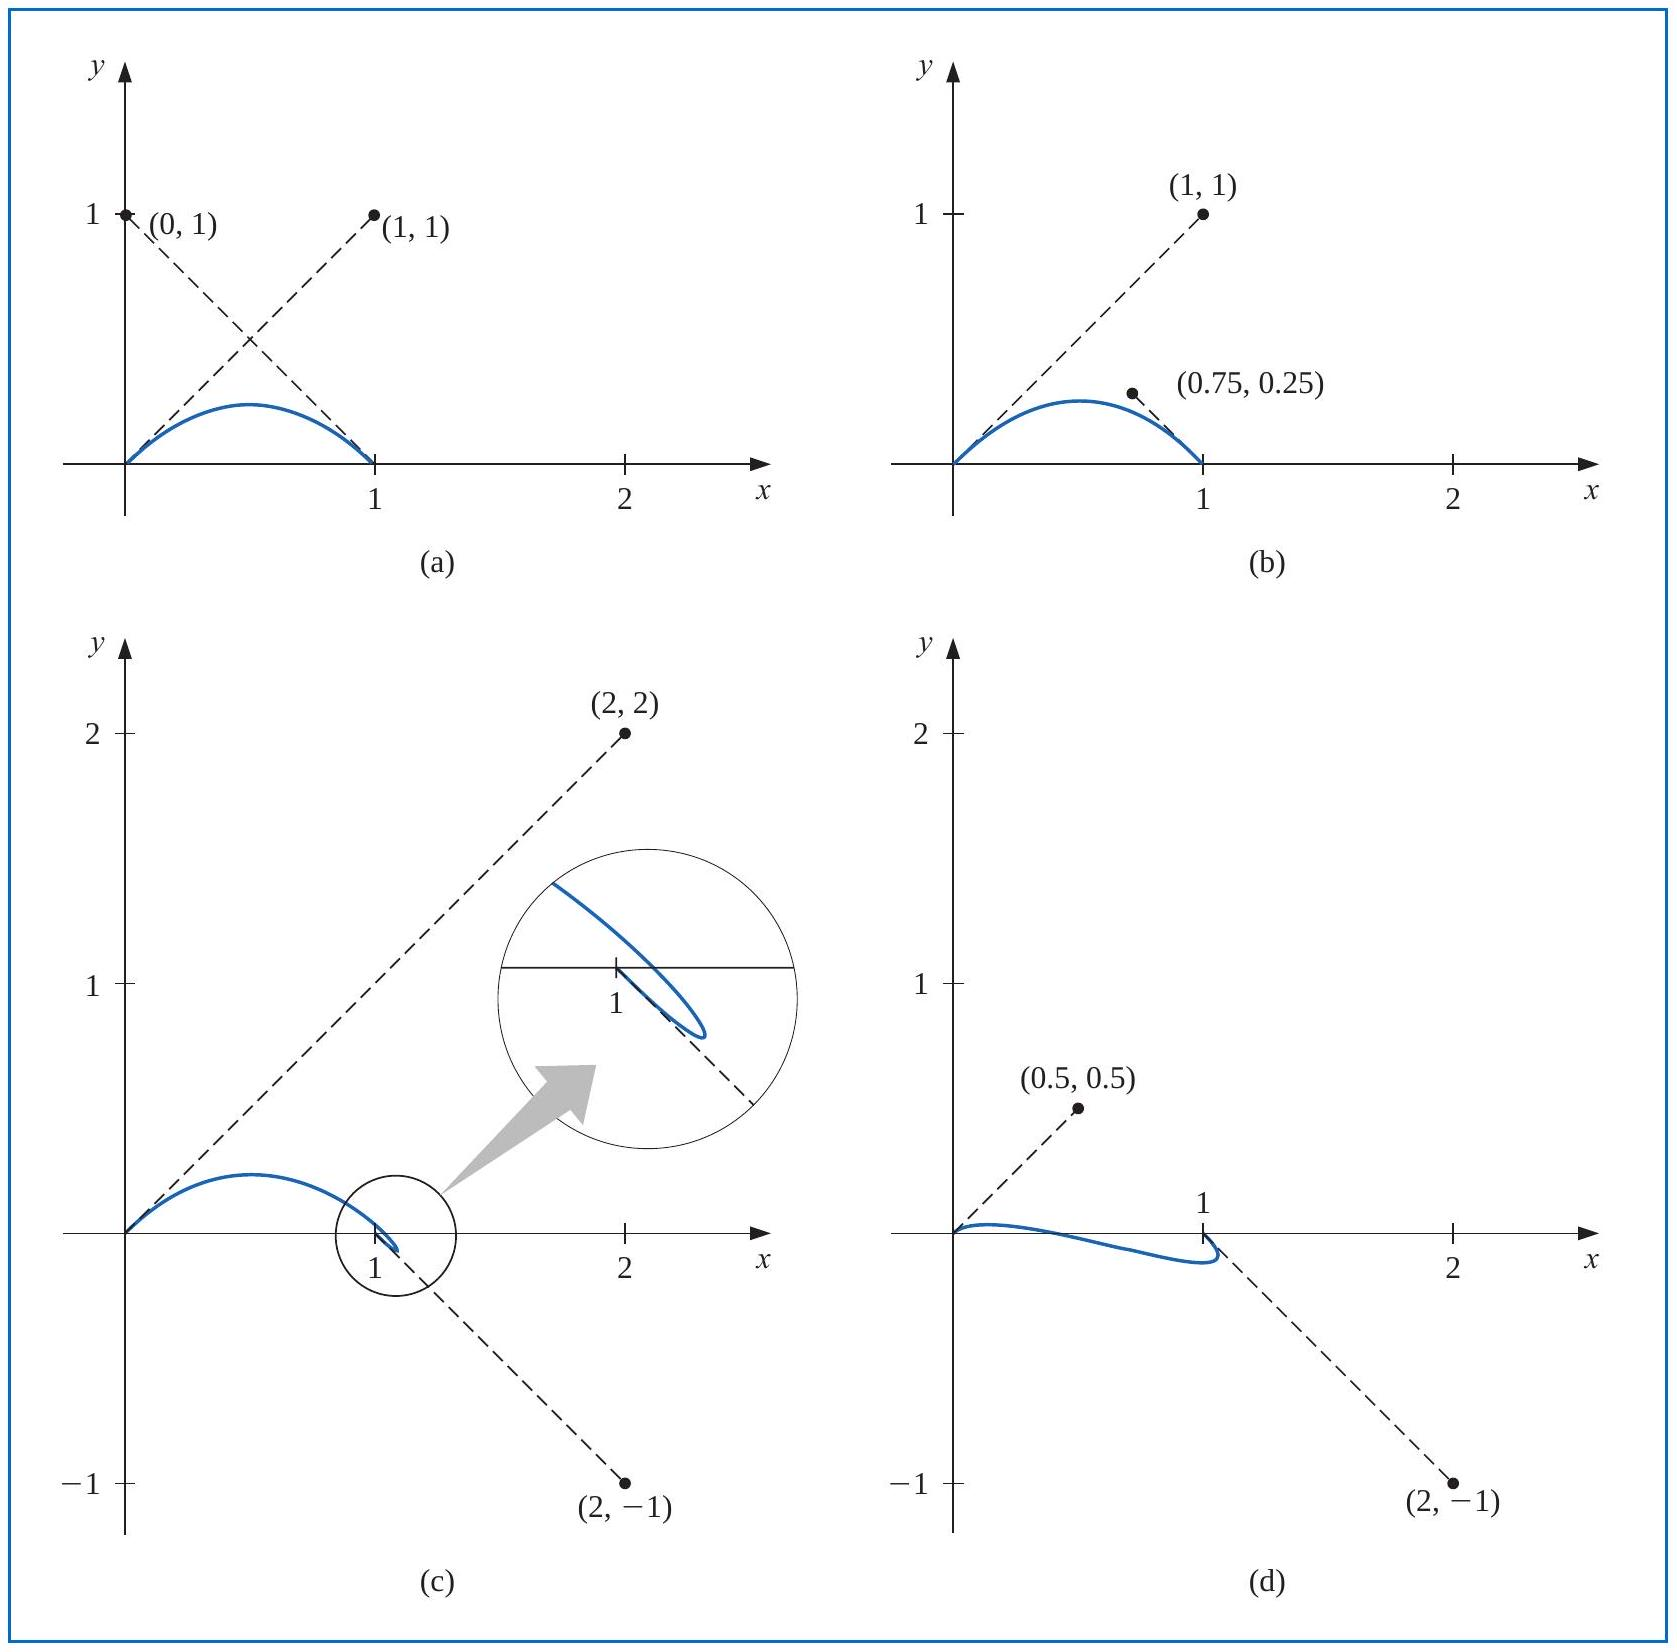
\includegraphics[width=13cm]{2025_05_15_4109a88b43049bd640d1g-64.JPG}
\caption{\scriptsize Figure $5$}
\label{fig:2025_05_15_4109a88b43049bd640d1g-64}
\end{figure}

%Pierre Etienne Bézier (1910-1999) was head of design and production for Renault motorcars for most of his professional life. He began his research into computer-aided design and manufacturing in 1960, developing interactive tools for curve and surface design, and initiated computer-generated milling for automobile modeling.
%
%The Bézier curves that bear his name have the advantage of being based on a rigorous mathematical theory that does not need to be explicitly recognized by the practitioner who simply wants to make an aesthetically pleasing curve or surface. These are the curves that are the basis of the powerful Adobe Postscript system, and produce the freehand curves that are generated in most sufficiently powerful computer graphics packages.\\
%\includegraphics[max width=\textwidth, center]{2025_05_15_4109a88b43049bd640d1g-65}
%
The standard procedure for determining curves in an interactive graphics mode is to first use a mouse or touchpad to set the nodes and guidepoints to generate a first approximation to the curve. These can be set manually, but most graphics systems permit you to use your input device to draw the curve on the screen freehand and will select appropriate nodes and guidepoints for your freehand curve.

The nodes and guidepoints can then be manipulated into a position that produces an aesthetically pleasing curve. Since the computation is minimal, the curve can be determined so quickly that the resulting change is seen immediately. Moreover, all the data needed to compute the curves are imbedded in the coordinates of the nodes and guidepoints, so no analytical knowledge is required of the user.

Popular graphics programs use this type of system for their freehand graphic representations in a slightly modified form. The Hermite cubics are described as {\bf Bézier polynomials}, which incorporate a scaling factor of $3$ when computing the derivatives at the endpoints. This modifies the parametric equations to


\begin{equation}\label{eqn:paramet3}
x(t)=\left[2\left(x_{0}-x_{1}\right)+3\left(\alpha_{0}+\alpha_{1}\right)\right] t^{3}+\left[3\left(x_{1}-x_{0}\right)-3\left(\alpha_{1}+2 \alpha_{0}\right)\right] t^{2}+3 \alpha_{0} t+x_{0}, 
\end{equation}


and


\begin{equation}\label{eqn:paramet4}
y(t)=\left[2\left(y_{0}-y_{1}\right)+3\left(\beta_{0}+\beta_{1}\right)\right] t^{3}+\left[3\left(y_{1}-y_{0}\right)-3\left(\beta_{1}+2 \beta_{0}\right)\right] t^{2}+3 \beta_{0} t+y_{0}, \tag{3.26}
\end{equation}


for $0 \leq t \leq 1$, but this change is transparent to the user of the system.

%Algorithm 3.6 constructs a set of Bézier curves based on the parametric equations in Eqs. (3.25) and (3.26).
%
%\section*{Bézier Curve}
%To construct the cubic Bézier curves $C_{0}, \ldots, C_{n-1}$ in parametric form, where $C_{i}$ is represented by
%
%$$
%\left(x_{i}(t), y_{i}(t)\right)=\left(a_{0}^{(i)}+a_{1}^{(i)} t+a_{2}^{(i)} t^{2}+a_{3}^{(i)} t^{3}, b_{0}^{(i)}+b_{1}^{(i)} t+b_{2}^{(i)} t^{2}+b_{3}^{(i)} t^{3}\right)
%$$
%
%for $0 \leq t \leq 1$, as determined by the left endpoint ( $x_{i}, y_{i}$ ), left guidepoint ( $x_{i}^{+}, y_{i}^{+}$), right endpoint ( $x_{i+1}, y_{i+1}$ ), and right guidepoint ( $x_{i+1}^{-}, y_{i+1}^{-}$) for each $i=0,1, \ldots, n-1$ :\\
%INPUT $n ;\left(x_{0}, y_{0}\right), \ldots,\left(x_{n}, y_{n}\right) ;\left(x_{0}^{+}, y_{0}^{+}\right), \ldots,\left(x_{n-1}^{+}, y_{n-1}^{+}\right) ;\left(x_{1}^{-}, y_{1}^{-}\right), \ldots,\left(x_{n}^{-}, y_{n}^{-}\right)$.\\
%OUTPUT coefficients $\left\{a_{0}^{(i)}, a_{1}^{(i)}, a_{2}^{(i)}, a_{3}^{(i)}, b_{0}^{(i)}, b_{1}^{(i)}, b_{2}^{(i)}, b_{3}^{(i)}\right.$, for $\left.0 \leq i \leq n-1\right\}$.\\
%Step 1 For each $i=0,1, \ldots, n-1$ do Steps 2 and 3 .\\
%Step 2 Set $a_{0}^{(i)}=x_{i}$;
%
%$$
%\begin{aligned}
%b_{0}^{(i)} & =y_{i} ; \\
%a_{1}^{(i)} & =3\left(x_{i}^{+}-x_{i}\right) ; \\
%b_{1}^{(i)} & =3\left(y_{i}^{+}-y_{i}\right) ; \\
%a_{2}^{(i)} & =3\left(x_{i}+x_{i+1}^{-}-2 x_{i}^{+}\right) ; \\
%b_{2}^{(i)} & =3\left(y_{i}+y_{i+1}^{-}-2 y_{i}^{+}\right) ; \\
%a_{3}^{(i)} & =x_{i+1}-x_{i}+3 x_{i}^{+}-3 x_{i+1}^{-} ; \\
%b_{3}^{(i)} & =y_{i+1}-y_{i}+3 y_{i}^{+}-3 y_{i+1}^{-} ;
%\end{aligned}
%$$
%
%Step 3 OUTPUT $\left(a_{0}^{(i)}, a_{1}^{(i)}, a_{2}^{(i)}, a_{3}^{(i)}, b_{0}^{(i)}, b_{1}^{(i)}, b_{2}^{(i)}, b_{3}^{(i)}\right)$.
%
%\section*{Step 4 STOP.}
%Three-dimensional curves are generated in a similar manner by additionally specifying third components $z_{0}$ and $z_{1}$ for the nodes and $z_{0}+\gamma_{0}$ and $z_{1}-\gamma_{1}$ for the guidepoints. The more difficult problem involving the representation of three-dimensional curves concerns the loss of the third dimension when the curve is projected onto a two-dimensional computer screen. Various projection techniques are used, but this topic lies within the realm of computer graphics. For an introduction to this topic and ways that the technique can be modified for surface representations, see one of the many books on computer graphics methods, such as [FVFH].
\begin{myexercise}%\label{Comprehensionquiz2}
Let $\left(x_{0}, y_{0}\right)=(0,0)$ and $\left(x_{1}, y_{1}\right)=(5,2)$ be the endpoints of a curve. Use the given guidepoints to construct parametric cubic Hermite approximations $(x(t), y(t))$ to the curve, and graph the approximations.

\begin{enumerate}[label=(\alph*)]
\item $(1,1)$ and $(6,1)$
\item $(1,1)$ and $(6,3)$
\item $(0.5, 0.5)$ and $(5.5, 1.5)$
\item $(2,2)$ and $(7,0)$
\end{enumerate}
\begin{mysolution}
\begin{enumerate}[label=(\alph*)]
\item $x(t)=-10t^3+14t^2+t$, $y(t)=-2t^3+3t^2+t$
\item $x(t)=-10t^3+14.5t^2+0.5t$, $y(t)=-3t^3+4.5t^2+0.5t$
\item $x(t)=-10t^3+14t^2+t$, $y(t)=-4t^3+5t^2+t$
\item $x(t)=-10t^3+13t^2+2t$, $y(t)=2t$
\end{enumerate}
\end{mysolution}
\end{myexercise}

\section{Numerical Diffrentiation}

\begin{youtube}
This video presents a discussion on numerical differentiation. Follow the discussion and then solve the problems in the subsequent quiz.
\end{youtube}
\mylink{https://www.youtube.com/watch?\\v=-3MwUJCDjts\&list=PLDea8VeK4MUTppAXQzHBNz3KiyEd9SQms\&index=82}

\mylink{https://www.youtube.com/watch?\\v=bKu\_MfpdUiQ\&list=PLDea8VeK4MUTppAXQzHBNz3KiyEd9SQms\&index=83}

\mylink{https://www.youtube.com/watch?\\v=VIXiLXYLjZY\&list=PLDea8VeK4MUTppAXQzHBNz3KiyEd9SQms\&index=84}

\mylink{https://www.youtube.com/watch?\\v=AvvvE3oqHDE\&list=PLDea8VeK4MUTppAXQzHBNz3KiyEd9SQms\&index=86}

\mylink{https://www.youtube.com/watch?v=AVvX-\\DyV3wQ\&list=PLDea8VeK4MUTppAXQzHBNz3KiyEd9SQms\&index=87}

\mylink{https://www.youtube.com/watch?\\v=RJhbUvyTBf0\&list=PLDea8VeK4MUTppAXQzHBNz3KiyEd9SQms\&index=88}

\mylink{https://www.youtube.com/watch?\\v=L\_80gD1TJSI\&list=PLDea8VeK4MUTppAXQzHBNz3KiyEd9SQms\&index=89}

Consider the following example

\begin{example} \label{numediffexample1}
Use the forward-difference formula to approximate the derivative of $f(x)=\ln x$ at $x_{0}=1.8$ using $h=0.1, h=0.05$, and $h=0.01$, and determine bounds for the approximation errors.
\end{example}
\begin{mysolution} 
The forward-difference formula

$$
\frac{f(1.8+h)-f(1.8)}{h}
$$

with $h=0.1$ gives

$$
\frac{\ln 1.9-\ln 1.8}{0.1}=\frac{0.64185389-0.58778667}{0.1}=0.5406722
$$

Because $f^{\prime \prime}(x)=-1 / x^{2}$ and $1.8<\xi<1.9$, a bound for this approximation error is

$$
\frac{\left|h f^{\prime \prime}(\xi)\right|}{2}=\frac{|h|}{2 \xi^{2}}<\frac{0.1}{2(1.8)^{2}}=0.0154321
$$

The approximation and error bounds when $h=0.05$ and $h=0.01$ are found in a similar manner and the results are shown in Table \ref{table1}.

%Table 4.1



Since $f^{\prime}(x)=1 / x$, the exact value of $f^{\prime}(1.8)$ is $0.55 \overline{5}$, and in this case the error bounds are quite close to the true approximation error.\qed
\end{mysolution}

\begin{figure}
\centering
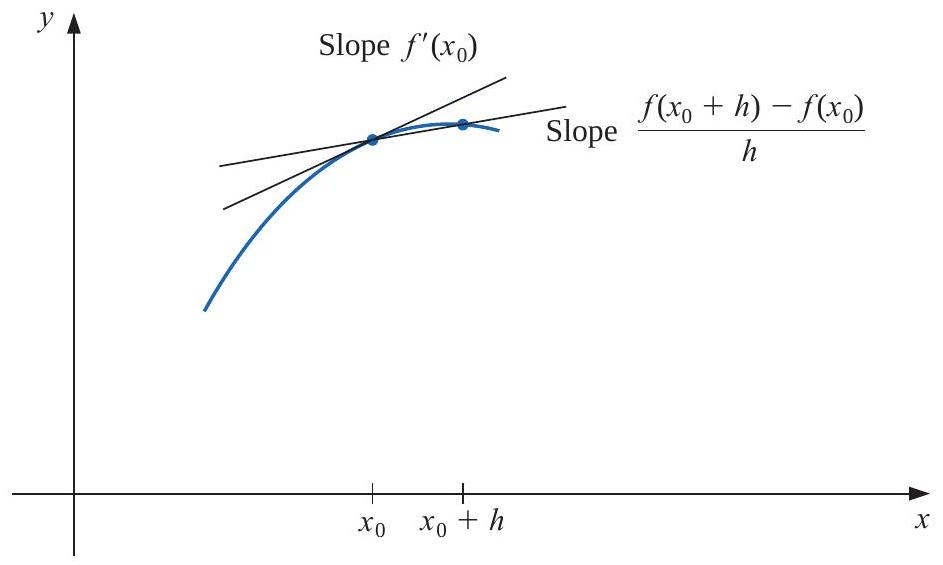
\includegraphics[width=10cm]{2025_05_15_85b7f7df47271a498e1dg-03}
\caption{\scriptsize Figure $6$}
\label{figure6}
\end{figure}

\begin{table}[h]
\centering
\begin{tabular}{lccc}
\hline
\multicolumn{1}{c}{$h$} & $f(1.8+h)$ & $\frac{f(1.8+h)-f(1.8)}{h}$ & $\frac{|h|}{2(1.8)^{2}}$ \\
\hline
0.1 & 0.64185389 & 0.5406722 & 0.0154321 \\
0.05 & 0.61518564 & 0.5479795 & 0.0077160 \\
0.01 & 0.59332685 & 0.5540180 & 0.0015432 \\
\hline
\end{tabular}
\caption{\scriptsize Table $1$}
\label{table1}
\end{table}

\begin{myexercise}%\label{Comprehensionquiz2}
Use the forward-difference formulas and backward-difference formulas to determine each missing entry in the following tables.
\begin{multicols}{2}
\begin{enumerate}[label=(\alph*)]
\item
\begin{center}
\begin{tabular}{c|c|l}
$x$ & $f(x)$ & $f^{\prime}(x)$ \\
\hline
0.5 & 0.4794 &  \\
0.6 & 0.5646 &  \\
0.7 & 0.6442 &  \\
\end{tabular}
\end{center}
\item
\begin{center}
\begin{tabular}{c|l|l}
$x$ & \multicolumn{1}{|c|}{$f(x)$} & $f^{\prime}(x)$ \\
\hline
0.0 & 0.00000 &  \\
0.2 & 0.74140 &  \\
0.4 & 1.3718 &  \\
\end{tabular}
\end{center}
\end{enumerate}
\end{multicols}
\begin{mysolution}
From the forward-backward difference formula we have the following approximations:
 \begin{enumerate}[label=(\alph*)]
\item $f'(0.5)\approx0.8520$, $f(0.6)\approx0.8520$, $f(0.7)\approx0.7960$
\item $f'(0.0)\approx3.7070$, $f(0.2)\approx3.1520$, $f(0.4\approx3.1520$
\end{enumerate}
\end{mysolution}
\end{myexercise}



\section{Richardson's Extrapolation}
\activities
Read on Richardson's extrapolation in the reference provided in the link below in the pages Appendix C1 and then attempt the subsequent quiz.
\begin{activity}[\cg Reading]
%\begin{enumerate}
%\item \mylink{https://math.libretexts.org/Bookshelves/Calculus/CLP-2\_Integral\_Calculus\_(Feldman\_Rechnitzer\_and\_Yeager)/04\%3A\_Appendices/4.03\%3A\_C\%3A\_More\_About\_Numerical\_Integration/4.3.01\%3A\_C.1\%3A\_Richardson\_Extrapolation}
%\end{enumerate}
\mylink{https://math.libretexts.org/Bookshelves/Calculus/\\CLP-2\_Integral\_Calculus\_(Feldman\_Rechnitzer\_and\_Yeager)}
\end{activity}

\begin{example}\label{Richardsonsexample1}
In Example \ref{numediffexample1} of Section 2 we use the forward-difference method with $h=0.1$ and $h=0.05$ to find approximations to $f^{\prime}(1.8)$ for $f(x)=\ln (x)$. Assume that this formula has truncation error $O(h)$ and use extrapolation on these values to see if this results in a better approximation.
\end{example}

\begin{mysolution}
In Example \ref{numediffexample1} of Section 2 we found that

$$
\text { with } h=0.1: f^{\prime}(1.8) \approx 0.5406722, \quad \text { and } \quad \text { with } h=0.05: f^{\prime}(1.8) \approx 0.5479795 .
$$

This implies that

$$
N_{1}(0.1)=0.5406722 \text { and } N_{1}(0.05)=0.5479795 .
$$

Extrapolating these results gives the new approximation

$$
\begin{aligned}
N_{2}(0.1) & =N_{1}(0.05)+\left(N_{1}(0.05)-N_{1}(0.1)\right)=0.5479795+(0.5479795-0.5406722) \\
& =0.555287
\end{aligned}
$$

The $h=0.1$ and $h=0.05$ results were found to be accurate to within $1.5 \times 10^{-2}$ and $7.7 \times 10^{-3}$, respectively. Because $f^{\prime}(1.8)=1 / 1.8=0 . \overline{5}$, the extrapolated value is accurate to within $2.7 \times 10^{-4}$.
\end{mysolution}
\begin{myexercise}%\label{Comprehensionquiz2}
Apply the extrapolation process described in Example \ref{Richardsonsexample1} to determine $N_{3}(h)$, an approximation to $f^{\prime}\left(x_{0}\right)$, for the following functions and stepsizes.
%%\begin{multicols}{2}
\begin{enumerate}[label=(\alph*)]
\item $\quad f(x)=\ln x, x_{0}=1.0, h=0.4$\\
\item $\quad f(x)=x+e^{x}, x_{0}=0.0, h=0.4$\\
\item $\quad f(x)=2^{x} \sin x, x_{0}=1.05, h=0.4$\\
\item $\quad f(x)=x^{3} \cos x, x_{0}=2.3, h=0.4$
\end{enumerate}
%\end{multicols}

\begin{mysolution}
\begin{multicols}{2}
\begin{enumerate}[label=(\alph*)]
\item $f(1)\approx1.0000109$ \item $f(0)\approx2.0000000$ \item $f(1.05)\approx2.2751459$ \item $f(2.3)\approx-19.646799$
\end{enumerate}
\end{multicols}
\end{mysolution}
\end{myexercise}


\section{Elements of Numerical Integration}
%\begin{youtube}
%This video presents a discussion on elements of numerical integration. Follow the discussion and then solve the problems in the subsequent quiz.
%\end{youtube}

\videolesson
\begin{selfvideo}[2]
%LESSON 3: 
This video presents a discussion on elements of numerical integration. Follow the discussion and then solve the problems in the subsequent quiz.
\end{selfvideo}

%\mylink{https://www.youtube.com/watch?v=2ypA51D945g\&list=PLDea8VeK4MUTppAXQzHBNz3KiyEd9SQms\&index=91}
%
%\mylink{https://www.youtube.com/watch?v=cE1WjwLTXMI\&list=PLDea8VeK4MUTppAXQzHBNz3KiyEd9SQms\&index=92}
%
%\mylink{https://www.youtube.com/watch?v=z8C1lXfsAC0\&list=PLDea8VeK4MUTppAXQzHBNz3KiyEd9SQms\&index=93}
%\begin{boxB}Question: \end{boxB}


The need often arises for evaluating the definite integral of a function that has no explicit antiderivative or whose antiderivative is not easy to obtain. The basic method involved in approximating $\int_{a}^{b} f(x) d x$ is called numerical quadrature. It uses a sum $\sum_{i=0}^{n} a_{i} f\left(x_{i}\right)$ to approximate $\int_{a}^{b} f(x) d x$.

The methods of quadrature in this section are based on the interpolation polynomials given in Chapter 3. The basic idea is to select a set of distinct nodes $\left\{x_{0}, \ldots, x_{n}\right\}$ from the interval $[a, b]$. Then integrate the Lagrange interpolating polynomial

$$
P_{n}(x)=\sum_{i=0}^{n} f\left(x_{i}\right) L_{i}(x)
$$

and its truncation error term over $[a, b]$ to obtain

$$
\begin{aligned}
\int_{a}^{b} f(x) d x & =\int_{a}^{b} \sum_{i=0}^{n} f\left(x_{i}\right) L_{i}(x) d x+\int_{a}^{b} \prod_{i=0}^{n}\left(x-x_{i}\right) \frac{f^{(n+1)}(\xi(x))}{(n+1)!} d x \\
& =\sum_{i=0}^{n} a_{i} f\left(x_{i}\right)+\frac{1}{(n+1)!} \int_{a}^{b} \prod_{i=0}^{n}\left(x-x_{i}\right) f^{(n+1)}(\xi(x)) d x
\end{aligned}
$$

where $\xi(x)$ is in $[a, b]$ for each $x$ and

$$
a_{i}=\int_{a}^{b} L_{i}(x) d x, \quad \text { for each } i=0,1, \ldots, n
$$

The quadrature formula is, therefore,

$$
\int_{a}^{b} f(x) d x \approx \sum_{i=0}^{n} a_{i} f\left(x_{i}\right)
$$

with error given by

$$
E(f)=\frac{1}{(n+1)!} \int_{a}^{b} \prod_{i=0}^{n}\left(x-x_{i}\right) f^{(n+1)}(\xi(x)) d x
$$

Before discussing the general situation of quadrature formulas, let us consider formulas produced by using first and second Lagrange polynomials with equally-spaced nodes. This gives the {\bf Trapezoidal rule} and {\bf Simpson's rule}, which are commonly introduced in calculus courses.

When we use the term trapezoid we mean a four-sided figure that has at least two of its sides parallel. The European term for this figure is trapezium. To further confuse the issue, the European word trapezoidal refers to a four-sided figure with no sides equal, and the American word for this type of figure is trapezium.

\subsection*{The Trapezoidal Rule}
To derive the Trapezoidal rule for approximating $\int_{a}^{b} f(x) d x$, let $x_{0}=a, x_{1}=b, h=b-a$ and use the linear Lagrange polynomial:

$$
P_{1}(x)=\frac{\left(x-x_{1}\right)}{\left(x_{0}-x_{1}\right)} f\left(x_{0}\right)+\frac{\left(x-x_{0}\right)}{\left(x_{1}-x_{0}\right)} f\left(x_{1}\right)
$$

Then


\begin{equation}\label{eqn:traprule1}
\begin{split}
\int_{a}^{b} f(x) d x= & \int_{x_{0}}^{x_{1}}\left[\frac{\left(x-x_{1}\right)}{\left(x_{0}-x_{1}\right)} f\left(x_{0}\right)+\frac{\left(x-x_{0}\right)}{\left(x_{1}-x_{0}\right)} f\left(x_{1}\right)\right] d x \\
& +\frac{1}{2} \int_{x_{0}}^{x_{1}} f^{\prime \prime}(\xi(x))\left(x-x_{0}\right)\left(x-x_{1}\right) d x 
\end{split}
\end{equation}


The product $\left(x-x_{0}\right)\left(x-x_{1}\right)$ does not change sign on $\left[x_{0}, x_{1}\right]$, so the Weighted Mean Value Theorem for Integrals 1.13 can be applied to the error term to give, for some $\xi$ in ( $x_{0}, x_{1}$ ),

$$
\begin{aligned}
\int_{x_{0}}^{x_{1}} f^{\prime \prime}(\xi(x))\left(x-x_{0}\right)\left(x-x_{1}\right) d x & =f^{\prime \prime}(\xi) \int_{x_{0}}^{x_{1}}\left(x-x_{0}\right)\left(x-x_{1}\right) d x \\
& =f^{\prime \prime}(\xi)\left[\frac{x^{3}}{3}-\frac{\left(x_{1}+x_{0}\right)}{2} x^{2}+x_{0} x_{1} x\right]_{x_{0}}^{x_{1}} \\
& =-\frac{h^{3}}{6} f^{\prime \prime}(\xi)
\end{aligned}
$$

Consequently, Eq. \ref{eqn:traprule1} implies that

$$
\begin{aligned}
\int_{a}^{b} f(x) d x & =\left[\frac{\left(x-x_{1}\right)^{2}}{2\left(x_{0}-x_{1}\right)} f\left(x_{0}\right)+\frac{\left(x-x_{0}\right)^{2}}{2\left(x_{1}-x_{0}\right)} f\left(x_{1}\right)\right]_{x_{0}}^{x_{1}}-\frac{h^{3}}{12} f^{\prime \prime}(\xi) \\
& =\frac{\left(x_{1}-x_{0}\right)}{2}\left[f\left(x_{0}\right)+f\left(x_{1}\right)\right]-\frac{h^{3}}{12} f^{\prime \prime}(\xi)
\end{aligned}
$$

Using the notation $h=x_{1}-x_{0}$ gives the following rule:\\

\begin{boxB}{\bf Trapezoidal Rule:}
$$
\int_{a}^{b} f(x) d x=\frac{h}{2}\left[f\left(x_{0}\right)+f\left(x_{1}\right)\right]-\frac{h^{3}}{12} f^{\prime \prime}(\xi)
$$
 \end{boxB}

This is called the Trapezoidal rule because when $f$ is a function with positive values, $\int_{a}^{b} f(x) d x$ is approximated by the area in a trapezoid, as shown in Figure \ref{fig:trapezoid1}.

%Figure 4.3\\
\begin{figure}[h]
\centering
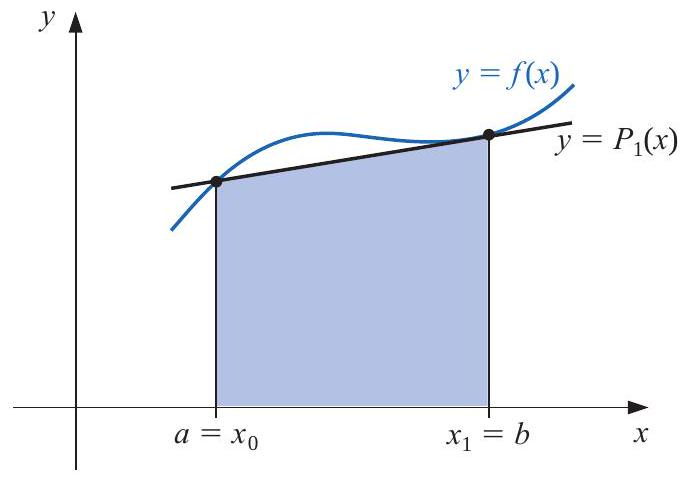
\includegraphics[width=10cm]{2025_05_15_85b7f7df47271a498e1dg-22}
\caption{\scriptsize Figure $7$}
\label{fig:trapezoid1}
\end{figure}

The error term for the Trapezoidal rule involves $f^{\prime \prime}$, so the rule gives the exact result when applied to any function whose second derivative is identically zero, that is, any polynomial of degree one or less.

\subsection*{Simpson's Rule}
Simpson's rule results from integrating over $[a, b]$ the second Lagrange polynomial with equally-spaced nodes $x_{0}=a, x_{2}=b$, and $x_{1}=a+h$, where $h=(b-a) / 2$. (See Figure \ref{fig:simpfig1}.)

%Figure 4.4\\
\begin{figure}[h]
\centering
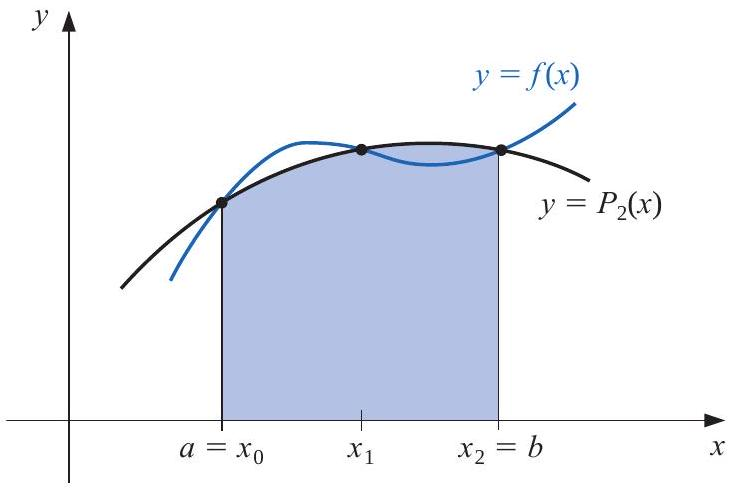
\includegraphics[width=10cm]{2025_05_15_85b7f7df47271a498e1dg-23}
\caption{\scriptsize Figure $8$}
\label{fig:simpfig1}
\end{figure}

Therefore

$$
\begin{aligned}
\int_{a}^{b} f(x) d x= & \int_{x_{0}}^{x_{2}}\left[\frac{\left(x-x_{1}\right)\left(x-x_{2}\right)}{\left(x_{0}-x_{1}\right)\left(x_{0}-x_{2}\right)} f\left(x_{0}\right)+\frac{\left(x-x_{0}\right)\left(x-x_{2}\right)}{\left(x_{1}-x_{0}\right)\left(x_{1}-x_{2}\right)} f\left(x_{1}\right)\right. \\
& \left.+\frac{\left(x-x_{0}\right)\left(x-x_{1}\right)}{\left(x_{2}-x_{0}\right)\left(x_{2}-x_{1}\right)} f\left(x_{2}\right)\right] d x \\
& +\int_{x_{0}}^{x_{2}} \frac{\left(x-x_{0}\right)\left(x-x_{1}\right)\left(x-x_{2}\right)}{6} f^{(3)}(\xi(x)) d x
\end{aligned}
$$

Deriving Simpson's rule in this manner, however, provides only an $O\left(h^{4}\right)$ error term involving $f^{(3)}$. By approaching the problem in another way, a higher-order term involving $f^{(4)}$ can be derived.

To illustrate this alternative method, suppose that $f$ is expanded in the third Taylor polynomial about $x_{1}$. Then for each $x$ in $\left[x_{0}, x_{2}\right]$, a number $\xi(x)$ in ( $x_{0}, x_{2}$ ) exists with\\
$f(x)=f\left(x_{1}\right)+f^{\prime}\left(x_{1}\right)\left(x-x_{1}\right)+\frac{f^{\prime \prime}\left(x_{1}\right)}{2}\left(x-x_{1}\right)^{2}+\frac{f^{\prime \prime \prime}\left(x_{1}\right)}{6}\left(x-x_{1}\right)^{3}+\frac{f^{(4)}(\xi(x))}{24}\left(x-x_{1}\right)^{4}$\\
and


\begin{equation}\label{eqn:simpson1}
\begin{split}
\int_{x_{0}}^{x_{2}} f(x) d x= & {\left[f\left(x_{1}\right)\left(x-x_{1}\right)+\frac{f^{\prime}\left(x_{1}\right)}{2}\left(x-x_{1}\right)^{2}+\frac{f^{\prime \prime}\left(x_{1}\right)}{6}\left(x-x_{1}\right)^{3}\right.} \\
& \left.+\frac{f^{\prime \prime \prime}\left(x_{1}\right)}{24}\left(x-x_{1}\right)^{4}\right]_{x_{0}}^{x_{2}}+\frac{1}{24} \int_{x_{0}}^{x_{2}} f^{(4)}(\xi(x))\left(x-x_{1}\right)^{4} d x 
\end{split}
\end{equation}


%Thomas Simpson (1710-1761) was a self-taught mathematician who supported himself during his early years as a weaver. His primary interest was probability theory, although in 1750 he published a two-volume calculus book entitled The Doctrine and Application of Fluxions.

Because $\left(x-x_{1}\right)^{4}$ is never negative on $\left[x_{0}, x_{2}\right]$, the Weighted Mean Value Theorem for Integrals 1.13 implies that

$$
\left.\frac{1}{24} \int_{x_{0}}^{x_{2}} f^{(4)}(\xi(x))\left(x-x_{1}\right)^{4} d x=\frac{f^{(4)}\left(\xi_{1}\right)}{24} \int_{x_{0}}^{x_{2}}\left(x-x_{1}\right)^{4} d x=\frac{f^{(4)}\left(\xi_{1}\right)}{120}\left(x-x_{1}\right)^{5}\right]_{x_{0}}^{x_{2}}
$$

for some number $\xi_{1}$ in ( $x_{0}, x_{2}$ ).\\
However, $h=x_{2}-x_{1}=x_{1}-x_{0}$, so

$$
\left(x_{2}-x_{1}\right)^{2}-\left(x_{0}-x_{1}\right)^{2}=\left(x_{2}-x_{1}\right)^{4}-\left(x_{0}-x_{1}\right)^{4}=0
$$

whereas

$$
\left(x_{2}-x_{1}\right)^{3}-\left(x_{0}-x_{1}\right)^{3}=2 h^{3} \quad \text { and } \quad\left(x_{2}-x_{1}\right)^{5}-\left(x_{0}-x_{1}\right)^{5}=2 h^{5} .
$$

Consequently, Eq. \ref{eqn:simpson1} can be rewritten as

$$
\int_{x_{0}}^{x_{2}} f(x) d x=2 h f\left(x_{1}\right)+\frac{h^{3}}{3} f^{\prime \prime}\left(x_{1}\right)+\frac{f^{(4)}\left(\xi_{1}\right)}{60} h^{5}
$$

If we now replace $f^{\prime \prime}\left(x_{1}\right)$ by the approximation given in Eq. (4.9) of Section 4.1, we have

$$
\begin{aligned}
\int_{x_{0}}^{x_{2}} f(x) d x & =2 h f\left(x_{1}\right)+\frac{h^{3}}{3}\left\{\frac{1}{h^{2}}\left[f\left(x_{0}\right)-2 f\left(x_{1}\right)+f\left(x_{2}\right)\right]-\frac{h^{2}}{12} f^{(4)}\left(\xi_{2}\right)\right\}+\frac{f^{(4)}\left(\xi_{1}\right)}{60} h^{5} \\
& =\frac{h}{3}\left[f\left(x_{0}\right)+4 f\left(x_{1}\right)+f\left(x_{2}\right)\right]-\frac{h^{5}}{12}\left[\frac{1}{3} f^{(4)}\left(\xi_{2}\right)-\frac{1}{5} f^{(4)}\left(\xi_{1}\right)\right]
\end{aligned}
$$

It can be shown by alternative methods that the values $\xi_{1}$ and $\xi_{2}$ in this expression can be replaced by a common value $\xi$ in ( $x_{0}, x_{2}$ ). This gives Simpson's rule.
\begin{boxB}
{\bf Simpson's Rule:}
$$
\int_{x_{0}}^{x_{2}} f(x) d x=\frac{h}{3}\left[f\left(x_{0}\right)+4 f\left(x_{1}\right)+f\left(x_{2}\right)\right]-\frac{h^{5}}{90} f^{(4)}(\xi)
$$
\end{boxB}

The error term in Simpson's rule involves the fourth derivative of $f$, so it gives exact results when applied to any polynomial of degree three or less.

\begin{example}
Compare the Trapezoidal rule and Simpson's rule approximations to $\int_{0}^{2} f(x) d x$ when $f(x)$ is\\
\begin{enumerate}[label=(\alph*)]
\begin{multicols}{3}
\item $x^{2}$
\item $x^{4}$
\item $(x+1)^{-1}$
\item $\sqrt{1+x^{2}}$
\item $\sin x$
\item $e^{x}$
\end{multicols}
\end{enumerate}
\end{example}
\begin{mysolution}
On [0,2] the Trapezoidal and Simpson's rule have the forms\\
Trapezoid: $\int_{0}^{2} f(x) d x \approx f(0)+f(2)$ and Simpson's: $\int_{0}^{2} f(x) d x \approx \frac{1}{3}[f(0)+4 f(1)+f(2)]$.

When $f(x)=x^{2}$ they give

$$
\begin{gathered}
\text { Trapezoid: } \int_{0}^{2} f(x) d x \approx 0^{2}+2^{2}=4 \text { and } \\
\text { Simpson's: } \int_{0}^{2} f(x) d x \approx \frac{1}{3}\left[\left(0^{2}\right)+4 \cdot 1^{2}+2^{2}\right]=\frac{8}{3}
\end{gathered}
$$

The approximation from Simpson's rule is exact because its truncation error involves $f^{(4)}$, which is identically 0 when $f(x)=x^{2}$.

The results to three places for the functions are summarized in Table \ref{tab:simpsonexample1}. Notice that in each instance Simpson's Rule is significantly superior.
\end{mysolution}
%Table 4.7

\begin{table}[h]
\centering
\begin{tabular}{|l|l|l|l|l|l|l|}
\hline
 & (a) & (b) & (c) & (d) & (e) & (f) \\
\hline
$f(x)$ & $x^{2}$ & $x^{4}$ & $(x+1)^{-1}$ & $\sqrt{1+x^{2}}$ & $\sin x$ & $e^{x}$ \\
\hline
Exact value & 2.667 & 6.400 & 1.099 & 2.958 & 1.416 & 6.389 \\
\hline
Trapezoidal & 4.000 & 16.000 & 1.333 & 3.326 & 0.909 & 8.389 \\
\hline
Simpson's & 2.667 & 6.667 & 1.111 & 2.964 & 1.425 & 6.421 \\
\hline
\end{tabular}
\caption{\scriptsize Table 2: Comparison of Trapezoid and Simpson's Rules }
\label{tab:simpsonexample1}
\end{table}


\subsection*{Measuring Precision}
The standard derivation of quadrature error formulas is based on determining the class of polynomials for which these formulas produce exact results. The next definition is used to facilitate the discussion of this derivation.

\begin{definition}\label{def:precision}
The degree of accuracy, or precision, of a quadrature formula is the largest positive integer $n$ such that the formula is exact for $x^{k}$, for each $k=0,1, \ldots, n$.
\end{definition}
%The improved accuracy of Simpson's rule over the Trapezoidal rule is intuitively explained by the fact that Simpson's rule includes a midpoint evaluation that provides better balance to the approximation.
%
%The open and closed terminology for methods implies that the open methods use as nodes only points in the open interval, ( $a, b$ ) to approximate $\int_{a}^{b} f(x) d x$. The closed methods include the points $a$ and $b$ of the closed interval $[a, b]$ as nodes.

Definition \ref{def:precision} implies that the Trapezoidal and Simpson's rules have degrees of precision one and three, respectively.

Integration and summation are linear operations; that is,

$$
\int_{a}^{b}(\alpha f(x)+\beta g(x)) d x=\alpha \int_{a}^{b} f(x) d x+\beta \int_{a}^{b} g(x) d x
$$

and

$$
\sum_{i=0}^{n}\left(\alpha f\left(x_{i}\right)+\beta g\left(x_{i}\right)\right)=\alpha \sum_{i=0}^{n} f\left(x_{i}\right)+\beta \sum_{i=0}^{n} g\left(x_{i}\right),
$$

for each pair of integrable functions $f$ and $g$ and each pair of real constants $\alpha$ and $\beta$. This implies that:

\begin{boxB}
The degree of precision of a quadrature formula is $n$ if and only if the error is zero for all polynomials of degree $k=0,1, \ldots, n$, but is not zero for some polynomial of degree $n+1$.
\end{boxB}

The Trapezoidal and Simpson's rules are examples of a class of methods known as NewtonCotes formulas. There are two types of Newton-Cotes formulas, open and closed.

\subsection*{Closed Newton-Cotes Formulas}
The ( $n+1$ )-point closed Newton-Cotes formula uses nodes $x_{i}=x_{0}+i h$, for $i=0,1, \ldots, n$, where $x_{0}=a, x_{n}=b$ and $h=(b-a) / n$. (See Figure \ref{fig:closednewtoncotes1}.) It is called closed because the endpoints of the closed interval $[a, b]$ are included as nodes.

%Figure 4.5\\
\begin{figure}[h]
\centering
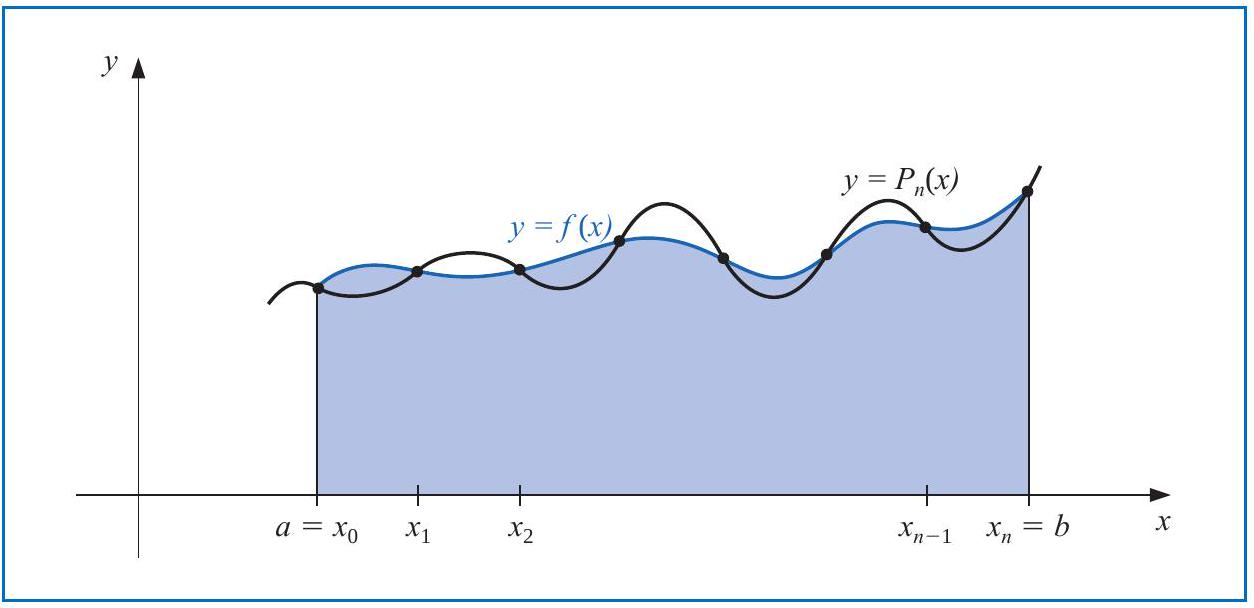
\includegraphics[width=12cm]{2025_05_15_85b7f7df47271a498e1dg-26}
\caption{\scriptsize Figure $9$}
\label{fig:closednewtoncotes1}
\end{figure}
The formula assumes the form

$$
\int_{a}^{b} f(x) d x \approx \sum_{i=0}^{n} a_{i} f\left(x_{i}\right)
$$

where

$$
a_{i}=\int_{x_{0}}^{x_{n}} L_{i}(x) d x=\int_{x_{0}}^{x_{n}} \prod_{\substack{j=0 \\ j \neq i}}^{n} \frac{\left(x-x_{j}\right)}{\left(x_{i}-x_{j}\right)} d x
$$

The following theorem details the error analysis associated with the closed Newton Cotes formulas.

\begin{theorem}\label{thm:closednewtonecotes}
Suppose that $\sum_{i=0}^{n} a_{i} f\left(x_{i}\right)$ denotes the ( $n+1$ )-point closed Newton-Cotes formula with $x_{0}=a, x_{n}=b$, and $h=(b-a) / n$. There exists $\xi \in(a, b)$ for which

%Roger Cotes (1682-1716) rose from a modest background to become, in 1704, the first Plumian Professor at Cambridge University. He made advances in numerous mathematical areas including numerical methods for interpolation and integration.\\
%Newton is reputed to have said of Cotes ...if he had lived we might have known something.

$$
\int_{a}^{b} f(x) d x=\sum_{i=0}^{n} a_{i} f\left(x_{i}\right)+\frac{h^{n+3} f^{(n+2)}(\xi)}{(n+2)!} \int_{0}^{n} t^{2}(t-1) \cdots(t-n) d t
$$

if $n$ is even and $f \in C^{n+2}[a, b]$, and

$$
\int_{a}^{b} f(x) d x=\sum_{i=0}^{n} a_{i} f\left(x_{i}\right)+\frac{h^{n+2} f^{(n+1)}(\xi)}{(n+1)!} \int_{0}^{n} t(t-1) \cdots(t-n) d t
$$

if $n$ is odd and $f \in C^{n+1}[a, b]$.
\end{theorem}

Note that when $n$ is an even integer, the degree of precision is $n+1$, although the interpolation polynomial is of degree at most $n$. When $n$ is odd, the degree of precision is only $n$.

Some of the common closed Newton-Cotes formulas with their error terms are listed. Note that in each case the unknown value $\xi$ lies in $(a, b)$.\\
{\bf $n=1$ : Trapezoidal rule}


\begin{equation}\label{eqn:closednewtontrap}
\int_{x_{0}}^{x_{1}} f(x) d x=\frac{h}{2}\left[f\left(x_{0}\right)+f\left(x_{1}\right)\right]-\frac{h^{3}}{12} f^{\prime \prime}(\xi), \quad \text { where } \quad x_{0}<\xi<x_{1} 
\end{equation}


{\bf $n=2$ : Simpson's rule}


\begin{equation}\label{eqn:closednewtonsim}
\int_{x_{0}}^{x_{2}} f(x) d x=\frac{h}{3}\left[f\left(x_{0}\right)+4 f\left(x_{1}\right)+f\left(x_{2}\right)\right]-\frac{h^{5}}{90} f^{(4)}(\xi), \quad \text { where } \quad x_{0}<\xi<x_{2} 
\end{equation}


{\bf $n=3$ : Simpson's Three-Eighths rule}


\begin{equation}\label{eqn:clsednewtonsimpsonnis3}
\int_{x_{0}}^{x_{3}} f(x) d x=\frac{3 h}{8}\left[f\left(x_{0}\right)+3 f\left(x_{1}\right)+3 f\left(x_{2}\right)+f\left(x_{3}\right)\right]-\frac{3 h^{5}}{80} f^{(4)}(\xi)
\end{equation}


where $\quad x_{0}<\xi<x_{3}$.\\
{\bf $n=4$ :}


\begin{equation}\label{eqn:clsednewtonsimpsonnis4}
\int_{x_{0}}^{x_{4}} f(x) d x=\frac{2 h}{45}\left[7 f\left(x_{0}\right)+32 f\left(x_{1}\right)+12 f\left(x_{2}\right)+32 f\left(x_{3}\right)+7 f\left(x_{4}\right)\right]-\frac{8 h^{7}}{945} f^{(6)}(\xi)
\end{equation}


\subsection*{Open Newton-Cotes Formulas}
The open Newton-Cotes formulas do not include the endpoints of $[a, b]$ as nodes. They use the nodes $x_{i}=x_{0}+i h$, for each $i=0,1, \ldots, n$, where $h=(b-a) /(n+2)$ and $x_{0}=a+h$. This implies that $x_{n}=b-h$, so we label the endpoints by setting $x_{-1}=a$ and $x_{n+1}=b$, as shown in Figure \ref{fig:opennewton1} on page 200. Open formulas contain all the nodes used for the approximation within the open interval $(a, b)$. The formulas become

$$
\int_{a}^{b} f(x) d x=\int_{x_{-1}}^{x_{n+1}} f(x) d x \approx \sum_{i=0}^{n} a_{i} f\left(x_{i}\right)
$$

where

$$
a_{i}=\int_{a}^{b} L_{i}(x) d x
$$


\begin{figure}[h]
\centering
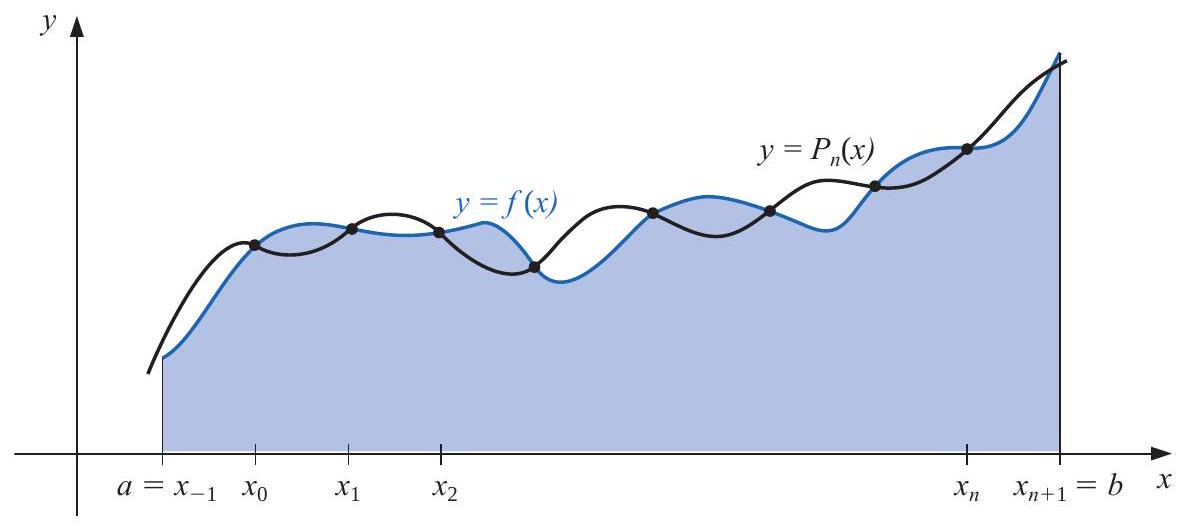
\includegraphics[width=12cm]{2025_05_15_85b7f7df47271a498e1dg-28}
\caption{\scriptsize Figure $10$}
\label{fig:opennewton1}
\end{figure}

The following theorem is analogous to Theorem \ref{thm:closednewtonecotes}

\begin{theorem}\label{thm:opennewtonecotes}
Suppose that $\sum_{i=0}^{n} a_{i} f\left(x_{i}\right)$ denotes the ( $n+1$ )-point open Newton-Cotes formula with $x_{-1}=a, x_{n+1}=b$, and $h=(b-a) /(n+2)$. There exists $\xi \in(a, b)$ for which

$$
\int_{a}^{b} f(x) d x=\sum_{i=0}^{n} a_{i} f\left(x_{i}\right)+\frac{h^{n+3} f^{(n+2)}(\xi)}{(n+2)!} \int_{-1}^{n+1} t^{2}(t-1) \cdots(t-n) d t
$$

if $n$ is even and $f \in C^{n+2}[a, b]$, and

$$
\int_{a}^{b} f(x) d x=\sum_{i=0}^{n} a_{i} f\left(x_{i}\right)+\frac{h^{n+2} f^{(n+1)}(\xi)}{(n+1)!} \int_{-1}^{n+1} t(t-1) \cdots(t-n) d t
$$

if $n$ is odd and $f \in C^{n+1}[a, b]$.
\end{theorem}

Notice, as in the case of the closed methods, we have the degree of precision comparatively higher for the even methods than for the odd methods.

Some of the common open Newton-Cotes formulas with their error terms are as follows:\\
{\bf $n=0$ : Midpoint rule}


\begin{equation}\label{eqn:opennewtoncotesmpnis0}
\int_{x_{-1}}^{x_{1}} f(x) d x=2 h f\left(x_{0}\right)+\frac{h^{3}}{3} f^{\prime \prime}(\xi), \quad \text { where } \quad x_{-1}<\xi<x_{1} 
\end{equation}


{\bf $n=1:$}


\begin{equation}\label{eqn:opennewtoncotesmpnis1}
\int_{x_{-1}}^{x_{2}} f(x) d x=\frac{3 h}{2}\left[f\left(x_{0}\right)+f\left(x_{1}\right)\right]+\frac{3 h^{3}}{4} f^{\prime \prime}(\xi), \quad \text { where } \quad x_{-1}<\xi<x_{2}
\end{equation}



{\bf $n=2:$}
\begin{equation}\label{eqn:opennewtoncotesmpnis2}
 \int_{x_{-1}}^{x_{3}} f(x) d x=\frac{4 h}{3}\left[2 f\left(x_{0}\right)-f\left(x_{1}\right)+2 f\left(x_{2}\right)\right]+\frac{14 h^{5}}{45} f^{(4)}(\xi) 
\end{equation}
 where  $ x_{-1}<\xi<x_{3}$.

{\bf $n=3$:}
\begin{equation}\label{eqn:opennewtoncotesmpnis3}
\int_{x_{-1}}^{x_{4}} f(x) d x=\frac{5 h}{24}\left[11 f\left(x_{0}\right)+f\left(x_{1}\right)+f\left(x_{2}\right)+11 f\left(x_{3}\right)\right]+\frac{95}{144} h^{5} f^{(4)}(\xi)
\end{equation}
where $x_{-1}<\xi<x_{4}$


\begin{example}
Compare the results of the closed and open Newton-Cotes formulas listed as \ref{eqn:closednewtontrap}-\ref{eqn:clsednewtonsimpsonnis4} and \ref{eqn:opennewtoncotesmpnis0}-\ref{eqn:opennewtoncotesmpnis3} when approximating

$$
\int_{0}^{\pi / 4} \sin x d x=1-\sqrt{2} / 2 \approx 0.29289322
$$
\end{example}

\begin{mysolution}
For the closed formulas we have

$$
\begin{aligned}
& n=1: \frac{(\pi / 4)}{2}\left[\sin 0+\sin \frac{\pi}{4}\right] \approx 0.27768018 \\
& n=2: \frac{(\pi / 8)}{3}\left[\sin 0+4 \sin \frac{\pi}{8}+\sin \frac{\pi}{4}\right] \approx 0.29293264 \\
& n=3: \frac{3(\pi / 12)}{8}\left[\sin 0+3 \sin \frac{\pi}{12}+3 \sin \frac{\pi}{6}+\sin \frac{\pi}{4}\right] \approx 0.29291070 \\
& n=4: \frac{2(\pi / 16)}{45}\left[7 \sin 0+32 \sin \frac{\pi}{16}+12 \sin \frac{\pi}{8}+32 \sin \frac{3 \pi}{16}+7 \sin \frac{\pi}{4}\right] \approx 0.29289318
\end{aligned}
$$

and for the open formulas we have

$$
\begin{array}{ll}
n=0: & 2(\pi / 8)\left[\sin \frac{\pi}{8}\right] \approx 0.30055887 \\
n=1: & \frac{3(\pi / 12)}{2}\left[\sin \frac{\pi}{12}+\sin \frac{\pi}{6}\right] \approx 0.29798754 \\
n=2: & \frac{4(\pi / 16)}{3}\left[2 \sin \frac{\pi}{16}-\sin \frac{\pi}{8}+2 \sin \frac{3 \pi}{16}\right] \approx 0.29285866 \\
n=3: & \frac{5(\pi / 20)}{24}\left[11 \sin \frac{\pi}{20}+\sin \frac{\pi}{10}+\sin \frac{3 \pi}{20}+11 \sin \frac{\pi}{5}\right] \approx 0.29286923
\end{array}
$$
\end{mysolution}
Table \ref{tab:intcomp} summarizes these results and shows the approximation errors.
%
%Table 4.8
%
\begin{table}[h]
\centering
\begin{tabular}{lccccc}
\hline
\multicolumn{1}{c}{$n$} & 0 & 1 & 2 & 3 & 4 \\
\hline
Closed formulas &  & 0.27768018 & 0.29293264 & 0.29291070 & 0.29289318 \\
Error &  & 0.01521303 & 0.00003942 & 0.00001748 & 0.00000004 \\
Open formulas & 0.30055887 & 0.29798754 & 0.29285866 & 0.29286923 &  \\
Error & 0.00766565 & 0.00509432 & 0.00003456 & 0.00002399 &  \\
\hline
\end{tabular}
\caption{\scriptsize Table 3: Comparison of Closed and Open Newton-Cotes Formulas}
\label{tab:intcomp}
\end{table}

\begin{myexercise}%\label{Comprehensionquiz2}
Consider the integral 
\[I=\int_1^{1.6}\frac{2x}{x^2-4}\,dx\]
\begin{enumerate}[label=(\alph*)]
\item Approximate the integral using the
\begin{enumerate}[label=\roman*.]
\item Trapezoidal rule
\item Simpson's rule
\item Midpoint rule
\end{enumerate}
\item Find abound for the error in each of the approximations in part (a) using the error formula, and compare this to the actual error.
\end{enumerate}

\begin{mysolution}
\begin{enumerate}[label=(\alph*)]
\item 
\begin{enumerate}[label=\roman*.]
\item $-0.8666667$
\item $-0.7391053$
\item $-0.6753247$
\end{enumerate}
\item 
\begin{enumerate}[label=\roman*.]
\item Actual error $=0.1326975$, Error bound $=0.5617284$
\item Actual error $= 5.1361\times10^{-3}$. Error bound $=0.063280$
\item Actual error $=0.0564448$, Error bound $=0.2808642$
\end{enumerate}
\end{enumerate}
\end{mysolution}
\end{myexercise}


%\discussion


\begin{posttest}%[\textcolor{red}{End of Module 4 Quiz}]
\item Construct and graph the cubic Bézier polynomials given the following points and guidepoints.
\begin{enumerate}[label=(\alph*)]
\item Point $(1,1)$ with guidepoint $(1.5,1.25)$ to point $(6,2)$ with guidepoint $(7,3)$\\
\item Point $(1,1)$ with guidepoint $(1.25,1.5)$ to point $(6,2)$ with guidepoint $(5,3)$\\
\item Point $(0,0)$ with guidepoint $(0.5,0.5)$ to point $(4,6)$ with entering guidepoint $(3.5,7)$ and exiting guidepoint $(4.5,5)$ to point $(6,1)$ with guidepoint $(7,2)$\\
\item Point $(0,0)$ with guidepoint $(0.5,0.5)$ to point $(2,1)$ with entering guidepoint $(3,1)$ and exiting guidepoint $(3,1)$ to point $(4,0)$ with entering guidepoint $(5,1)$ and exiting guidepoint $(3,-1)$ to point $(6,-1)$ with guidepoint $(6.5,-0.25)$ 
\end{enumerate}

\item Conside the data and the corresponding function that generated the data. Compute the actual errors, and find error bounds using the error formulas.

\begin{multicols}{2}
\begin{enumerate}[label=(\alph*)]
\item
\begin{center}
\begin{tabular}{c|c|l}
$x$ & $f(x)$ & $f^{\prime}(x)$ \\
\hline
0.5 & 0.4794 &  \\
0.6 & 0.5646 &  \\
0.7 & 0.6442 &  \\
\end{tabular}
\end{center}

\[f(x)=\sin x\]
\item
\begin{center}
\begin{tabular}{c|l|l}
$x$ & \multicolumn{1}{|c|}{$f(x)$} & $f^{\prime}(x)$ \\
\hline
0.0 & 0.00000 &  \\
0.2 & 0.74140 &  \\
0.4 & 1.3718 &  \\
\end{tabular}
\end{center}

 \[f(x)=e^{x}-2 x^{2}+3 x-1\]
\end{enumerate}
\end{multicols}

\item Apply the extrapolation process described in Example \ref{Richardsonsexample1} to determine $N_{3}(h)$, an approximation to $f^{\prime}\left(x_{0}\right)$, using four-digit rounding arithmetic for the following functions and stepsizes.
%%\begin{multicols}{2}
\begin{enumerate}[label=(\alph*)]
\item $\quad f(x)=\ln x, x_{0}=1.0, h=0.4$\\
\item $\quad f(x)=x+e^{x}, x_{0}=0.0, h=0.4$\\
\item $\quad f(x)=2^{x} \sin x, x_{0}=1.05, h=0.4$\\
\item $\quad f(x)=x^{3} \cos x, x_{0}=2.3, h=0.4$
\end{enumerate}
%\end{multicols}
\item Consider the integral 
\[I=\int_0^{\pi/4}e^{3x}\sin2x\,dx\]
\begin{enumerate}[label=(\alph*)]
\item Approximate the integral using the
\begin{enumerate}[label=\roman*.]
\item Trapezoidal rule
\item Simpson's rule
\item Midpoint rule
\end{enumerate}
\item Find abound for the error in each of the approximations in part (a) using the error formula, and compare this to the actual error.
\end{enumerate}

\begin{mysolution}
\begin{enumerate}[label=\arabic*.]
\item
\begin{enumerate}[label=(\alph*)]
\item $x(t)=-11.5t^3+15t^2+1.5t+1$, $y(t)=-4.25t^3+4.5t^2+0.75t+1$
\item $x(t)=-6.25t^3+10.5t^2+0.75t+1$, $y(t)=-3.5t^3+3t^2+1.5t+1$
\item For $t$ between $(0,0)$ and $(4,6)$, we have
\[x(t) =-5t^3 +7.5t^2 +1.5t,\quad y(t) =-13.5t^3 +18t^2 +1.5t,\]
and for $t$ between $(4,6)$ and $(6,1)$, we have
\[x(t) =-5.5t^3 + 6t^2 +1.5t +4,\quad y(t) = 4t^3 -6t^2-3t +6.\]
\item For t between $(0,0)$ and $(2,1)$, we have
\[x(t) =-5.5t^3 + 6t^2 +1.5t,\quad y(t) =-0.5t^3 +1.5t,\]
for $t$ between $(2,1)$ and $(4,0)$, we have
\[x(t) =-4t^3 +3t^2 +3t +2,\quad y(t) =-t^3 +1,\]
and for $t$ between $(4,0)$ and $(6,-1)$, we have
\[x(t) =-8.5t^3 + 13.5t^2-3t +4,\quad y(t) =-3.25t^3 +5.25t^2-3t.\]
\end{enumerate}
\item
\begin{center}
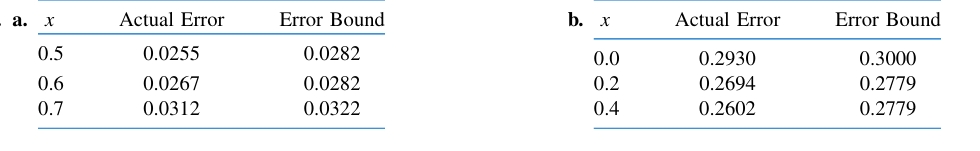
\includegraphics[width=15cm]{EndofMod4Q2sol}
\end{center}
\item
\begin{multicols}{2}
\begin{enumerate}[label=(\alph*)]
\item $f(1)\approx1.001$ \item $f(0)\approx1.999$ \item $f(1.05)\approx2.283$ \item $f(2.3)\approx-19.61$
\end{enumerate}
\end{multicols}
\item 
\begin{enumerate}[label=(\alph*)]
\item 
\begin{enumerate}[label=\roman*.]
\item $4.1432597$
\item $2.5836964$
\item $1.8039148$
\end{enumerate}
\item 
\begin{enumerate}[label=\roman*.]
\item Actual error $=1.554631$, Error bound $=2.298827$
\item Actual error $= 4.9322\times10^{-3}$. Error bound $=0.1302826$
\item Actual error $=0.7847138$, Error bound $=1.1494136$
\end{enumerate}
\end{enumerate}
\end{enumerate}
\end{mysolution}
\end{posttest}

%share your understanding of properties of functions and their applications to solving rates of change problems in physical phenomenon 


%\end{actsoln}

\takehome

\comy{You are now at the last part of this module. Your  task is to do a self-reflection on your learning experience.}



\references
\begin{refenumerate}
\item Kong, Q., Siauw, T., Bayen, A., (2020). Python Programming and Numerical Methods. First Edition, Academic Press,  ISBN-13 ‏ : ‎ 978-0128195499 \\
%chapter 1 pg 7-36 functions\\
%chapter 1 pg 51-83 limits and continuity\\
%chapter 1 pg 45-50 rates of change\\
%chapter 2 pg 108-120 the derivative\\
%\item Mendelson, E. (2022). Schaum's Outline of Calculus. McGraw-Hill Education.
%chapter 6 51-55 functions
%chapter 7 59-65 limits
%chapter 8 69-74 continuity
%chapter 9 77-81 derivative
%\item Calculus \mylink{https://math.libretexts.org/Bookshelves/Calculus}
%\item Chris McMullen, 2021, Essential Calculus Skills Practice Workbook with Full Solutions, Zishka Publishing, ISBN 978-1-941691-24-3
%\item R. Adams and C. Essex, 2021, Calculus: A complete Course, Addison Wesley, ISBN 13: 978-0135732588
%\item P. Abbott and H. Neill, 2018, Calculus: A Complete Introduction: The Easy Way to Learn Calculus (Teach Yourself), ISBN 13: 978-1473678446
\end{refenumerate}





%\wrapup
%To wrap-up, answer the following questions:
%
%\begin{enumerate}
%\item 
%%when do we say that a limit of a function exists?
%%\item how do we remove discontinuity in functions?
%%\item what is the relationship between the gradient of the tangent line and the derivative?
%\end{enumerate}
















%\newpage

%\facilitation


%
\begin{center}
    {\Large \textbf{FUNCTIONS OF SEVERAL VARIABLES}}\\[2mm]
(DEFINITION, DOMAIN, RANGE, GRAPHS AND LEVEL CURVES) \\[4mm]

\mycenterbox{5 minute review}%\\[4mm]
Recap the definition of a function of several variables, and the meaning of domain, range, graph and level curves of functions of several variables.
\end{center}
\mycenterbox{Warm-up.}%\\[4mm]
\problemAnswer{
Match the function with its graph (labeled I–VI).Give reasons for your choices
\begin{multicols}{3}
\begin{enumerate}[label=(\alph*)]
\item $f(x,y)=|x|+|y|$\\[4mm]
\item $f(x,y)=|xy|$
\item $f(x,y)=\frac{1}{1+x^2+y^2}$\\2mm]
\item $f(x,y)=(x^2-y^2)^2$
\item $f(x,y)=(x-y)^2$\\[4mm]
\item $f(x,y)=\sin(|x|+|y|)$
\end{enumerate}
\end{multicols}

\begin{center}
%\centering
\includegraphics[width=10cm]{MCTutorial1Q1.JPEG}
\end{center}
%\tcbox[tcbox raise base]{Warm-up}
 
%\begin{flushright}
%\begin{tikzpicture}
%    % A body
%
%
%    % Non-rectangle shapes must be drawn as polygone
%    \begin{scope}[shift={(3,0)}]
%        \draw  (0,0.5) -- (0,4) -- (.5,4) -- (.5,4.5) -- (1.,4.5) -- (4.,4.5) --(4.,4)-- (4.5,4) --(4.5,0.5) --(4.0,0.5)--(4.0,0.0)-- (.5,0) --(0.5,0.5) -- cycle;
%        % Draw symmetry lines
%        \draw [symmetry] (.5, 0.5) -- (.5,4.0);
%        \draw [symmetry] (4, 0.5) -- (4,4.0);
%        \draw [symmetry] (.5,4.0) -- (4,4.0);
%         \draw [symmetry] (.5, 0.5) -- (4, 0.5);
%        % Dimensions
%        \draw (4.5,0) -- ++(0.5,0) coordinate (D1) -- +(5pt,0);
%        \draw (4.5,4.5) -- ++(0.5,0) coordinate (D2) -- +(5pt,0);
%        \draw [dimen] (D1) -- (D2) node {6cm};
%       
%        
%        \draw (0.0,5) -- ++(0,0.5) coordinate (D1) -- +(0,+5pt);
%        \draw (0.5,5) -- ++(0,0.5) coordinate (D2) -- +(0,+5pt);
%        \draw [dimen,-] (D1) -- (D2) node [above=5pt] {$x$ cm};
%        \draw [dimen,<-] (D1) -- ++(-5pt,0);
%        \draw [dimen,<-] (D2) -- ++(+5pt,0);
%    \end{scope}
%\end{tikzpicture}
%\end{flushright}

}


\mycenterbox{Problems.}%

%\begin{center}
%\tcbox[tcbox raise base]{ Problems. Choose from the below}
%\end{center}
\problem{Exploring functions}%
\begin{enumerate}[(a)]
\item Are the following functions even, odd, or neither? What can you say
about their range?
\begin{multicols}{4}
 \begin{enumerate}[(i)]
\item $\displaystyle \frac{3x}{x^2+2}$
\item $\displaystyle \cos x+3$
\item $\displaystyle \frac{2x^3}{\cos x+3}$
\item $\displaystyle \frac{3x^4+2x^2}{\sin x+4}$
\end{enumerate}
\end{multicols}
\item Consider the functions $\sin^n x$ and $\cos^n x$, where $n$ is a positive integer.
Which are odd, which are even, and what are their periodicities?
\item What is the periodicity of $f(x) = 2 \cos x+\sin 2x$? Is it even/odd/neither?

\end{enumerate}

\problem{Cubic functions} 
Show that $x-1$ is a factor of the cubic function%
$$P(x)=x^3-2x^2-5x+6,$$
and  find the quadratic factor $Q(x)$ such that $P(x) = (x -1)Q(x)$. Factorise
$Q(x)$ and hence sketch $P(x).$

%\newpage
\problem{Sigmoid functions*.}%
For positive integers $n$, consider the family of functions
$$\displaystyle f_n= \frac{x^n}{2^n+x^n}.$$
\begin{enumerate}[(a)]
\item What are appropriate domains and ranges for $f_n(x)$? Do they depend on $n$?

\item Is $f_n(x)$ even, odd, or neither? Does this depend on $n$?

\item Show that for $x\geq 0$, $f_n(x)$ are strictly increasing functions and that
$0\leq f_n(x) < 1.$
\item What is the value of $f_n(2)$? Does it depend on $n$?

\item By considering the values of $f_n(1.9)$ and $f_n(2.1)$ for $n = 2, 4, 8, 16, 32$ and
$64$, show that the graph of $f_n(x)$ for $x\ge 0$ is an increasing sigmoid (that
is, $S$-shaped) function that approaches a step function as $n\rightarrow \infty$.
\end{enumerate}

\mycenterbox{Selected answers and hints}%

For the warm-up, $V(x)=4x(3-x)^2$. Writing $x=1+\epsilon$, we get
$$V = 4(1 +\epsilon)(3- (1+\epsilon))^2=4(4-\epsilon^2(3-\epsilon)).$$
If $-1<\epsilon<2$ then $\epsilon^2 (3-\epsilon)\ge 0$, with equality when $\epsilon=0$. Thus the maximum
value of $V$ occurs when $\epsilon= 0$, i.e. $x = 1\rm{cm}$.

\begin{enumerate}
\item 
\begin{enumerate}[(i)]
\item Odd. The range is the interval  $[-\frac{3}{4}\sqrt{2},\; \frac{3}{4}\sqrt{2}]$
\item Even. The range is the interval $[2, 4]$.
\item Odd. The range is all of $\mathbb R$.
\item Neither. (For example, writing $\displaystyle \frac{5}{\sin x+4}$ we have $\displaystyle f(1)= \frac{5}{\sin (1)+4} \equiv 1.032 (3\rm{dp})$ which is neither $f(1)$ nor $-f(1)$.)\\[4mm]
The range is the nonnegative reals $[0,\infty)$

\end{enumerate}
\end{enumerate}











%
%\newpage
%
%\newpage
%
%
%\newtheorem{definition}[subsection]{Definition}
%\newtheorem{example}[subsection]{Example}
\newtheorem{cor}[subsection]{Corollary}
\newtheorem{pro}[subsection]{Proposition}
\newtheorem{theo}[subsection]{Theorem}
\newtheorem{lem}[subsection]{Lemma}
%\newtheorem{rem}[subsection]{Remark}

\definecolor{main}{HTML}{5989cf}    % setting main color to be used
\definecolor{sub}{HTML}{cde4ff}     % setting sub color to be used

\tcbset{
    sharp corners,
    colback = white,
    before skip = 0.2cm,    % add extra space before the box
    after skip = 0.5cm      % add extra space after the box
}                           % setting global options for tcolorbox

% You can copy any following box you like to your code.
\newtcolorbox{boxA}{
    fontupper = \bf,
    boxrule = 1.5pt,
    colframe = black % frame color
}

\newtcolorbox{boxB}{
    fontupper = \bf\color{main}, % font color
    boxrule = 1.5pt,
    colframe = main,
    rounded corners,
    arc = 5pt   % corners roundness
}
\newtcolorbox{boxC}{
    colback = sub, % background color
    boxrule = 0pt  % no borders
}

\newtcolorbox{boxD}{
    colback = sub, 
    colframe = main, 
    boxrule = 0pt, 
    toprule = 3pt, % top rule weight
    bottomrule = 3pt % bottom rule weight
}

\hypersetup{
    colorlinks=true,
    linkcolor=blue,
    filecolor=magenta,      
    urlcolor=cyan,
    pdftitle={Overleaf Example},
    pdfpagemode=FullScreen,
    }

\urlstyle{same}


\coursetitle{\mtthreeiii}{MT303}
\developers{Wyclife Rao}
\reviewers{Dr. Irene Sitawa}
\modulenumber{5}
\modulename{Numerical Integration}

% courses
\thispagestyle{empty}
\begin{tikzpicture}[overlay,remember picture,font=\sffamily\bfseries]
 \draw[ultra thick,c4,name path=big arc] ([xshift=-2mm]current page.north) arc(150:285:11) coordinate[pos=0.225] (x0);
 \begin{scope}
  \clip ([xshift=-2mm]current page.north) arc(150:285:11) --(current page.north east);
  \fill[c4!50,opacity=0.25] ([xshift=4.55cm]x0) circle (4.55);
  \fill[c4!50,opacity=0.25] ([xshift=3.4cm]x0) circle (3.4);
  \fill[c4!50,opacity=0.25] ([xshift=2.25cm]x0) circle (2.25);
  \draw[ultra thick,c4!50] (x0) arc(-90:30:6.5);
  \draw[ultra thick,c4] (x0) arc(90:-30:8.75);
  \draw[ultra thick,c4!50,name path=arc1] (x0) arc(90:-90:4.675);
  \draw[ultra thick,c4!50] (x0) arc(90:-90:2.875);
  \path[name intersections={of=big arc and arc1,by=x1}];
  \draw[ultra thick,c4,name path=arc2] (x1) arc(135:-20:4.75);
  \draw[ultra thick,c4!50] (x1) arc(135:-20:8.75);
  \path[name intersections={of=big arc and arc2,by={aux,x2}}];
  \draw[ultra thick,c4!50] (x2) arc(180:50:2.25);
 \end{scope} 
 \path[decoration={text along path,text color=c4,
                 raise = -2.8ex,
                 text  along path,
                 text = {},%|\sffamily\bfseries|02/18/2019
                 text align = center,
             },
             decorate
         ] ([xshift=-2mm]current page.north) arc(150:245:11);
 %
 \newcommand\add{4cm}
 \begin{scope}%[shift={(5,0)}]
  \path[clip,postaction={fill=c3}]
  ([xshift=2cm+\add,yshift=-8cm]current page.center) rectangle ++ (4.6,7.7);
  \draw[c5,ultra thick,fill=c2] ([xshift=0.5cm+\add,yshift=-8cm]current page.center)
   ([xshift=0.5cm+\add,yshift=-8cm]current page.center)  arc(180:60:2)
    |- ++ (-3,6) --cycle;
  \draw[ultra thick,c5] ([xshift=-1.5cm+\add,yshift=-8cm]current page.center) 
  arc(180:0:2);
  \draw[ultra thick,c5] ([xshift=0.5cm+\add,yshift=-8cm]current page.center) 
  arc(180:0:2);
  \draw[ultra thick,c5] ([xshift=2.5cm+\add,yshift=-8cm]current page.center) 
  arc(180:0:2);
  \draw[ultra thick,c5] ([xshift=4.5cm+\add,yshift=-8cm]current page.center) 
  arc(180:0:2);
  \fill[white] ([xshift=2.5cm+\add,yshift=-8cm]current page.center) +(60:2) circle(1.5mm)
  node[above
  right=0mm,text=c5!80!black]{$\rho:=\dfrac{1+\sqrt{-3}}{2}$};
 \end{scope}
 %
 \fill[c1] ([xshift=2cm+\add,yshift=-8cm]current page.center) rectangle ++ (-30.7,7.7);
 \node[text=white,anchor=west,scale=2.3,inner sep=0pt] at
 ([xshift=-10cm,yshift=-1.8cm]current page.center) {\color{ulabgold} LEARNING};
 \node[text=white,anchor=west,scale=5,inner sep=0pt] at
 ([xshift=-10cm,yshift=-3.25cm]current page.center) {MODULE \dpmdnumber};
 \node[text=white,anchor=west,scale=2.5,inner sep=0pt,text width=.4\textwidth] at
 ([xshift=-10cm,yshift=-6cm]current page.center) {\dpmdname};
 \node[text=white,anchor=east,scale=2,inner sep=0pt] at
 ([xshift=5.7cm,yshift=-7.5cm]current page.center) {\color{ulabgold}The Open University of Kenya};
 %
% \draw[gray,line width=5mm] 
% ([xshift=2mm,yshift=-1mm]current page.south west) rectangle ([xshift=-2mm,yshift=1mm]current
% page.north east);
\end{tikzpicture}

%\newpage
\pagenumbering{roman}
\thispagestyle{empty}%firstpage


\begin{center}
\vspace*{2cm}
{\Huge\bf BACHELOR OF TECHNOLOGY EDUCATION}\\[3cm]  


%{\fontsize{80}{40}\selectfont \dpcoursecode}\\[2cm]
%
%{\fontsize{30}{40} \selectfont \dpcoursename}\\[2cm]

%\rule{\textwidth}{1pt}
%\vspace{2cm}

%{\fontsize{40}{40}\selectfont \bf Module~\dpmdnumber}\\[2cm]
%
%{\fontsize{30}{40}\selectfont \bf \dpmdname}\\

\vfill
\begin{flushright}
\begin{minipage}{.6\textwidth}
\begin{tcolorbox}%[text ]
\begin{tabular}{ll}%\hline
\subtitle{Developed by:}&\displaydevelopers\\
&\\
\subtitle{Reviewed by:}&\makecell[l]{\displayreviewers}\\
\end{tabular}
\end{tcolorbox}
\end{minipage}\hspace*{-3.5cm}
\end{flushright}
\vspace*{-2.5cm}
\end{center}

\newpage
\thispagestyle{empty}
\null
\vfill
{\renewcommand\arraystretch{1.5}
\begin{tabular}{|l|l|}\hline
\subtitle{Programme Title} & Bachelor of Technology Education \\\hline
\subtitle{Course Title} & \fullcoursename\\\hline
\subtitle{Learning Module number} & Module \dpmdnumber\\\hline
\subtitle{Learning module title} & \dpmdname \\\hline
\subtitle{Module Developer} & \displaydevelopers\\\hline
\subtitle{Reviewed by} & \displayreviewers\\\hline
%\subtitle{Vision} & \vision\\\hline
%\subtitle{Audience description} & \\\hline
\end{tabular}}
\clearpage

%\section{COURSE LEARNING GUIDE}


\subsection*{Preparing for Online and Distance Learning}

This course offers you the opportunity to enter an online space where you can engage with fellow students at the university. The online forums, exercises, tasks and materials have been designed by the course facilitators in such a way that you can draw directly from their knowledge and share in their scholarly interest in online learning and assessment

We hope you will use your access to this virtual classroom to raise all your questions on the course module, to build a network great learners and to share your own thoughts and experiences to the benefit of your fellow students.

   
There are a number of steps you can take to ensure you are well prepared to make the most of this learning opportunity. This resource should prompt you to consider the following:


 \begin{enumerate}[label=\cb$\square$]
   \item How can you best prepare the space where you expect you will spend most of your time engaging in online learning (i.e. in your home or office, or even during your commute to work or whilst traveling)?
  \item   What can you do to ensure you keep working through the course material, even when you do not have Internet access?
    \item How can you familiarise yourself with the course layout, in order to be able to navigate through the steps with ease?
    \item What are the communication strategies and best practices you could consider to best engage with your fellow students and the course facilitators?
    \item What do you do when you need academic or technical support?

 \end{enumerate} 

\subsection*{General Module Guide}

The authors of this module believe that imparting knowledge should always be a mutual relationship between the students and the teachers. Students can actively construct knowledge through experiences gained in reading and answering the learning modules.

You should take time to read everything written in the module, actively and religiously solve all the exercises included to finish this course and be able to gain all the competencies and skills expected to demonstrate the learning outcomes as stated in this course. If you finish with full confidence that you understand and can apply all the knowledge you gain in this course, then you are sure to succeed in tackling the next higher subjects in your chosen course.

In this course, you will be taught not only the knowledge you need to demonstrate your learning outcomes, but you will also gain discipline, perseverance, higher thinking skills, and resourcefulness that would help strengthen your foundation to succeed in life. To successfully finish the course, you must follow the guides set forth in using this module.


\begin{description}[{format=\textcolor{ulabblue}}]
\item[STUDY ENVIRONMENT.]\leavevmode\\
Before engaging into the module, make sure that you are comfortable enough and diminish distractions. Make sure that you develop a study routine to perform and accomplish all the activities set forth by the module.
%\newpage

\item[MODE OF DELIVERY.]\leavevmode\\
Students are required to get a access a digitised copy of the module from the Virtue Learning Environment. As an open and distance learner, you should be able to learn independently and optimise the learning modes and environment available to you as much of  the delivery of all the lessons will be done asynchronously. Your success will greatly depend on your self-motivation and discipline to get your work done without your instructor to remind you from time to time.

\item[STUDY SCHEDULE.] \leavevmode\\
Remember that you have other subjects to attend to, hence, you must manage your time so that you will not be left behind in any of them. Create your own learning plan for each course to make sure that you can perform all the activities. Do not procrastinate your work, remember that time wasted can never be retrieved back. Make sure that even if you are at home, you are a student enrolled in a program, where the learning of all its courses greatly depends on your will to learn as the materials you need are all in your hands. So always be aware of your daily tasks.

\item[PRACTICE EXERCISE.]\leavevmode\\
To measure your learning from your reading, you are given practice exercises which you are supposed to answer daily. This will prepare you in performing your main task.

\item[ONLINE GROUP CHAT.]\leavevmode\\
I am going to create an online Discussion Forum and QA Forum  on the VLE.  This will serve as a room for discussion on the topics and activities found in your module.

\item[RECOMMENDED REFERENCES FOR SUPPLEMENTARY READING.]\leavevmode\\
You are given links that you need to access online. These links are online references such as e-books, online activities, and tutorial videos of the topic. These are other references you can use to further understand the topic and gain additional knowledge and skills.

\item[MAIN TASK.]\leavevmode\\
You are given a task that will require you to apply the knowledge and skills you learned from the module. This can be a group or individual activity which will measure your higher order thinking skills you acquired throughout the topic.

\item[RUBRICS. ]\leavevmode\\
This is a tool to guide you in performing your main task. Through this, you will be able to know the specific indicators that should be found in your task. This is to assess your constructive behaviour towards your learning application. You will be rated according to a 4-point scale shown below.
\begin{center}
{\color{ulabgold} \bf 4 − Excellent\quad\quad   3 −Good\quad\quad    2 − Fair \quad\quad  1 −Poor}
\end{center}
\item[REFLECTIONS.]\leavevmode\\
Writing your reflection will be a passageway to express your experiential learning in using this module. In your honest recall, write everything that you think happened to you during your learning experience in this module. Use the guide questions below:
\begin{description}[{format=\textcolor{ulabblue}}]
\item[First paragraph. ]\leavevmode\\
How was your learning experience? Maybe you can consider describing the effect of the parts of the module (sequence, discussions, examples, practice exercises, online activities, and the main task) in your learning experience. You can point out the strength and weakness of each part so that we can consider it for future improvement of this instructional material.
\item[Second paragraph.  ]\leavevmode\\
What did you learn? Did you successfully acquire the learning outcomes?

\item[Third paragraph.]\leavevmode\\
How can you use what you learned in the future?
\end{description}
\end{description}

\section{ASSESSMENT  TASKS \& EXAMINATION   RULES AND GUIDELINES}

\begin{enumerate}[label=\cb\arabic*.]
\item {\cb SUBMISSION OF ASSESSMENT TASTS.}

Since mathematical skills are best acquired through constant practice, you are encouraged to answer at least two (2) exercises a day. These practice exercises will not be graded but it will help you develop your thinking skills which will prepare you in the performance of your main tasks. You are required to submit your practice exercises every week.
\begin{center} {\cg Usually submission deadlines are set on Saturday 11:59PM EAT} \end{center}

\item  {\cb GROUP CHAT.}

You can post questions, solutions, and comment to other's post. Please be reminded that our group chat is exclusive only for discussion on topics related to this course. Everyone is required to actively participate in the discussions. Also, trolling is highly discouraged. Always observe proper online etiquettes when participating in discussions.
\begin{center} {\cb RULE OF THUMB: ALWAYS THINK BEFORE YOU CLICK} \end{center}

\item  {\cb MAIN TASK. }

Complete documentation during the preparation of your task is required to ensure that every member of the group participated and contributed in the task. May it be photos or screenshots of your virtual meetings or group works. You are going to submit it as attachment of your main task the same way as the practice exercises.



\item {\cb RECOMMENDED REFERENCES FOR SUPPLEMENTARY READING.} 

You can explore online for other references that is related to the topic to gain additional information about the topic. Do not share or post inappropriate materials online or even privately.
\end{enumerate}

\subsection*{Requirements to pass the course}

Compiled Continuous  Assignment/Activities and Tasks  with Final Performance Examination.

\subtitle{Grading System}
\begin{center}
{\renewcommand\arraystretch{1.5}
\begin{tabular}{|l|c|}\hline
Continuous Activities and Tasks  &  50\%\\\hline
Final Performance Examination. &  50\%\\\hline
\end{tabular}
}
\end{center}
%\newpage










%\subsection{INTRODUCTORY MESSAGE}

%A warm welcome to \;  \fullcoursename, {\bf Module on \dpmdname}.



%By this module learning resource, we aim to enable you  achieve the relevant competencies, depict skill, action and purpose successfully. 
 

%It has been designed to provide you with fun and meaningful opportunities for guided and independent learning at your own pace and time. You will be enabled to process the contents of the learning material while being an active learner. Your academic success lies in your own hands.  This module has the following parts and corresponding icons:





{
\renewcommand\arraystretch{4}
\begin{longtblr}{
width=\linewidth,
 colspec={ Q[1,c,f] Q[1.5,r,m] Q[4,l,m] },
%row{1} = { font=\bfseries },
% rowhead = 1,
  caption={ }, 
  label={ },
  rowsep = 4pt,
  hlines = {ulabblue!20, 1pt},
  vlines = {ulabblue!20, 1pt},
}

\includegraphics[width=2cm]{img/audience} & {\bf AUDIENCE}  &  This is a description of a target audience.   \\
{\fontsize{40}{30}\selectfont\color{ulabblue}\faCogs}& {\bf MODULE DESCRIPTION} & 
This part explains the importance of the topics discussed in the module. It will also give you a sneak peek of what you will learn and what is expected from you at the end of the module.\\

\includegraphics[width=2cm]{img/target.png} &  {\bf  EXPECTATION} & These are what you will be able to know after completing the lessons in the module\\

\includegraphics[width=2cm]{img/preactivities} & {\bf PRE-ACTIVITY} &
This activity is to get you set, activate and engage schema to learn the module. Through this activity, you will know the relevance of this activity to the topic that will be discussed in the module.\\

\includegraphics[width=2cm]{img/pretest} &  {\bf PRE - ASSESSMENT} & This will measure your prior knowledge and the concepts to be mastered throughout the lesson. \\

\includegraphics[width=1.7cm]{img/rewind} &  {\bf  RECAP} & This section will measure what learnings and skills that you understand from the previous lesson.\\

\includegraphics[width=1.5cm]{img/lesson} &  {\bf  LESSON} & This section will discuss the topic for this module.\\

\includegraphics[width=2cm]{img/activities} &  {\bf  ACTIVITIES} & This is a set of activities you will perform.\\

\includegraphics[width=2cm]{img/summary} &  {\bf  WRAP UP} & This section summarizes the concepts and applications of the lessons.\\

\includegraphics[width=2cm]{img/discussion}& {\bf DISCUSSIONS} &
This is the meat of the module. The discussion is aligned to the topic learning outcomes that is expected of you to acquire at the end of the module.\\

\includegraphics[width=1.8cm]{img/value} &  {\bf  VALUING} & This part will check the integration of values in the learning competency you will take home.\\

\includegraphics[width=1.8cm]{img/posttest} &  {\bf  POST - ASSESSMENT} & This will measure how much you have learned from the entire module.\\

\includegraphics[width=1.8cm]{img/selfreflect} & {\bf REFLECTION }
&
This part is for you to share your thoughts by writing your reflection, make sure to check your grammar and spelling to ensure the readability and so that it will not alter the thought being delivered. 
\end{longtblr}
}









%\vfill

\audience
\begin{oldactivity}{Audience Description}{
\includegraphics[width=22mm]{img/audience}}{}
This module is offered to all students taking the Bachelor of Technology Education. As an open and distance learner, you should be able to learn independently and optimise the learning modes and environment available to you. Before you begin this course, please confirm the course material, the course requirements and how the course is conducted.
\end{oldactivity}
%\newpage
\pagenumbering{arabic}



\mddescription
This module guides you into a detailed discussion of the concepts of numerical integration. Specificcally you will learn about
\begin{itemize}
\item composite numerical integration
\item Romberg integration
\item adaptive quadrature methods
\item Gaussian quadrature 
\end{itemize}
\expectations
%\begin{objenumerate}
%
%\end{objenumerate}

\begin{mlos}
\item Define the principles of Romberg integration and Gaussian quadrature.
\item Explain adaptive quadrature and its advantages over fixed-step methods.
\item Implement Romberg and Gaussian quadrature methods to approximate definite integrals.
\item Apply the concepts of efficiency and accuracy of different numerical integration techniques in deciding numerical methods to use in specific cases.
\end{mlos}

\section{Composite Numerical Integration}
\videolesson
\begin{selfvideo}[1]
%LESSON 3: 
This video presents a discussion on composite numerical integration. Follow the discussion and then solve the problems in the subsequent quiz.
\end{selfvideo}
%\begin{boxB}Question: \end{boxB}
The Newton-Cotes formulas are generally unsuitable for use over large integration intervals. High-degree formulas would be required, and the values of the coefficients in these formulas are difficult to obtain. Also, the Newton-Cotes formulas are based on interpolatory polynomials that use equally-spaced nodes, a procedure that is inaccurate over large intervals because of the oscillatory nature of high-degree polynomials.

In this section, we discuss a piecewise approach to numerical integration that uses the low-order Newton-Cotes formulas. These are the techniques most often applied.

\begin{example}
Use Simpson's rule to approximate $\int_{0}^{4} e^{x} d x$ and compare this to the results obtained by adding the Simpson's rule approximations for $\int_{0}^{2} e^{x} d x$ and $\int_{2}^{4} e^{x} d x$. Compare these approximations to the sum of Simpson's rule for $\int_{0}^{1} e^{x} d x, \int_{1}^{2} e^{x} d x, \int_{2}^{3} e^{x} d x$, and $\int_{3}^{4} e^{x} d x$.
\end{example}

\begin{mysolution}
Simpson's rule on $[0,4]$ uses $h=2$ and gives

$$
\int_{0}^{4} e^{x} d x \approx \frac{2}{3}\left(e^{0}+4 e^{2}+e^{4}\right)=56.76958
$$

The exact answer in this case is $e^{4}-e^{0}=53.59815$, and the error -3.17143 is far larger than we would normally accept.

Applying Simpson's rule on each of the intervals $[0,2]$ and $[2,4]$ uses $h=1$ and gives

$$
\begin{aligned}
\int_{0}^{4} e^{x} d x & =\int_{0}^{2} e^{x} d x+\int_{2}^{4} e^{x} d x \\
& \approx \frac{1}{3}\left(e^{0}+4 e+e^{2}\right)+\frac{1}{3}\left(e^{2}+4 e^{3}+e^{4}\right) \\
& =\frac{1}{3}\left(e^{0}+4 e+2 e^{2}+4 e^{3}+e^{4}\right) \\
& =53.86385
\end{aligned}
$$

The error has been reduced to $-0.26570$.

For the integrals on $[0,1],[1,2],[3,4]$, and $[3,4]$ we use Simpson's rule four times with $h=\frac{1}{2}$ giving

$$
\begin{aligned}
\int_{0}^{4} e^{x} d x= & \int_{0}^{1} e^{x} d x+\int_{1}^{2} e^{x} d x+\int_{2}^{3} e^{x} d x+\int_{3}^{4} e^{x} d x \\
\approx & \frac{1}{6}\left(e_{0}+4 e^{1 / 2}+e\right)+\frac{1}{6}\left(e+4 e^{3 / 2}+e^{2}\right) \\
& +\frac{1}{6}\left(e^{2}+4 e^{5 / 2}+e^{3}\right)+\frac{1}{6}\left(e^{3}+4 e^{7 / 2}+e^{4}\right) \\
= & \frac{1}{6}\left(e^{0}+4 e^{1 / 2}+2 e+4 e^{3 / 2}+2 e^{2}+4 e^{5 / 2}+2 e^{3}+4 e^{7 / 2}+e^{4}\right) \\
= & 53.61622
\end{aligned}
$$

The error for this approximation has been reduced to -0.01807 .\qed
\end{mysolution}

To generalize this procedure for an arbitrary integral $\int_{a}^{b} f(x) d x$, choose an even integer $n$. Subdivide the interval $[a, b]$ into $n$ subintervals, and apply Simpson's rule on each consecutive pair of subintervals. (See Figure \ref{fig:2025_05_15_85b7f7df47271a498e1dg-32})


\begin{figure}[h]
\centering
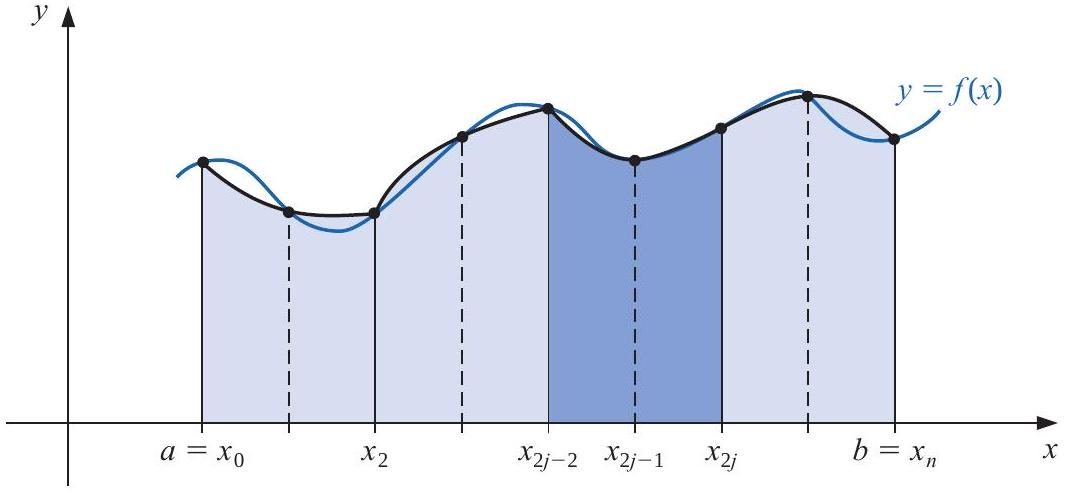
\includegraphics[width=12cm]{2025_05_15_85b7f7df47271a498e1dg-32.JPG}
\caption{\scriptsize Figure $1$}
\label{fig:2025_05_15_85b7f7df47271a498e1dg-32}
\end{figure}

With $h=(b-a) / n$ and $x_{j}=a+j h$, for each $j=0,1, \ldots, n$, we have

$$
\begin{aligned}
\int_{a}^{b} f(x) d x & =\sum_{j=1}^{n / 2} \int_{x_{2 j-2}}^{x_{2 j}} f(x) d x \\
& =\sum_{j=1}^{n / 2}\left\{\frac{h}{3}\left[f\left(x_{2 j-2}\right)+4 f\left(x_{2 j-1}\right)+f\left(x_{2 j}\right)\right]-\frac{h^{5}}{90} f^{(4)}\left(\xi_{j}\right)\right\}
\end{aligned}
$$

for some $\xi_{j}$ with $x_{2 j-2}<\xi_{j}<x_{2 j}$, provided that $f \in C^{4}[a, b]$. Using the fact that for each $j=1,2, \ldots,(n / 2)-1$ we have $f\left(x_{2 j}\right)$ appearing in the term corresponding to the interval $\left[x_{2 j-2}, x_{2 j}\right]$ and also in the term corresponding to the interval $\left[x_{2 j}, x_{2 j+2}\right]$, we can reduce this sum to

$$
\int_{a}^{b} f(x) d x=\frac{h}{3}\left[f\left(x_{0}\right)+2 \sum_{j=1}^{(n / 2)-1} f\left(x_{2 j}\right)+4 \sum_{j=1}^{n / 2} f\left(x_{2 j-1}\right)+f\left(x_{n}\right)\right]-\frac{h^{5}}{90} \sum_{j=1}^{n / 2} f^{(4)}\left(\xi_{j}\right)
$$

The error associated with this approximation is

$$
E(f)=-\frac{h^{5}}{90} \sum_{j=1}^{n / 2} f^{(4)}\left(\xi_{j}\right)
$$

where $x_{2 j-2}<\xi_{j}<x_{2 j}$, for each $j=1,2, \ldots, n / 2$.

%If $f \in C^{4}[a, b]$, the Extreme Value Theorem implies that $f^{(4)}$ assumes its maximum and minimum in $[a, b]$. Since
%
%$$
%\min _{x \in[a, b]} f^{(4)}(x) \leq f^{(4)}\left(\xi_{j}\right) \leq \max _{x \in[a, b]} f^{(4)}(x)
%$$
%
%we have
%
%$$
%\frac{n}{2} \min _{x \in[a, b]} f^{(4)}(x) \leq \sum_{j=1}^{n / 2} f^{(4)}\left(\xi_{j}\right) \leq \frac{n}{2} \max _{x \in[a, b]} f^{(4)}(x)
%$$
%
%and
%
%$$
%\min _{x \in[a, b]} f^{(4)}(x) \leq \frac{2}{n} \sum_{j=1}^{n / 2} f^{(4)}\left(\xi_{j}\right) \leq \max _{x \in[a, b]} f^{(4)}(x)
%$$
%
%By the Intermediate Value Theorem 1.11, there is a $\mu \in(a, b)$ such that
%
%$$
%f^{(4)}(\mu)=\frac{2}{n} \sum_{j=1}^{n / 2} f^{(4)}\left(\xi_{j}\right)
%$$
%
%Thus
%
%$$
%E(f)=-\frac{h^{5}}{90} \sum_{j=1}^{n / 2} f^{(4)}\left(\xi_{j}\right)=-\frac{h^{5}}{180} n f^{(4)}(\mu)
%$$
%
%or, since $h=(b-a) / n$,
%
%$$
%E(f)=-\frac{(b-a)}{180} h^{4} f^{(4)}(\mu)
%$$

These observations produce the following result.

\begin{theorem}
Let $f \in C^{4}[a, b], n$ be even, $h=(b-a) / n$, and $x_{j}=a+j h$, for each $j=0,1, \ldots, n$. There exists a $\mu \in(a, b)$ for which the Composite Simpson's rule for $n$ subintervals can be written with its error term as

$$
\int_{a}^{b} f(x) d x=\frac{h}{3}\left[f(a)+2 \sum_{j=1}^{(n / 2)-1} f\left(x_{2 j}\right)+4 \sum_{j=1}^{n / 2} f\left(x_{2 j-1}\right)+f(b)\right]-\frac{b-a}{180} h^{4} f^{(4)}(\mu)
$$
\end{theorem}
Notice that the error term for the Composite Simpson's rule is $O\left(h^{4}\right)$, whereas it was $O\left(h^{5}\right)$ for the standard Simpson's rule. However, these rates are not comparable because for standard Simpson's rule we have $h$ fixed at $h=(b-a) / 2$, but for Composite Simpson's rule we have $h=(b-a) / n$, for $n$ an even integer. This permits us to considerably reduce the value of $h$ when the Composite Simpson's rule is used.
%
%Algorithm 4.1 uses the Composite Simpson's rule on $n$ subintervals. This is the most frequently used general-purpose quadrature algorithm.
%
%\section*{Composite Simpson's Rule}
%To approximate the integral $I=\int_{a}^{b} f(x) d x$ :\\
%INPUT endpoints $a, b$; even positive integer $n$.\\
%OUTPUT approximation $X I$ to $I$.\\
%Step 1 Set $h=(b-a) / n$.\\
%Step 2 Set XIO $=f(a)+f(b)$;\\
%XI1 $=0 ; \quad$ (Summation of $\left.f\left(x_{2 i-1}\right).\right)$\\
%XI2 $=0 . \quad$ (Summation of $f\left(x_{2 i}\right)$. )\\
%Step 3 For $i=1, \ldots, n-1$ do Steps 4 and 5.\\
%Step 4 Set $X=a+i h$.\\
%Step 5 If $i$ is even then set $X I 2=X I 2+f(X)$\\
%else set $X I 1=X I 1+f(X)$.\\
%Step 6 Set $X I=h(X I 0+2 \cdot X I 2+4 \cdot X I 1) / 3$.\\
%Step 7 OUTPUT (XI);\\
%STOP.

The subdivision approach can be applied to any of the Newton-Cotes formulas. The extensions of the Trapezoidal (see Figure 4.8) and Midpoint rules are given without proof. The Trapezoidal rule requires only one interval for each application, so the integer $n$ can be either odd or even.

\begin{theorem}
Let $f \in C^{2}[a, b], h=(b-a) / n$, and $x_{j}=a+j h$, for each $j=0,1, \ldots, n$. There exists a $\mu \in(a, b)$ for which the {\bf Composite Trapezoidal rule} for $n$ subintervals can be written with its error term as

$$
\int_{a}^{b} f(x) d x=\frac{h}{2}\left[f(a)+2 \sum_{j=1}^{n-1} f\left(x_{j}\right)+f(b)\right]-\frac{b-a}{12} h^{2} f^{\prime \prime}(\mu)
$$
\end{theorem}

\newpage
\begin{figure}[h]
\centering
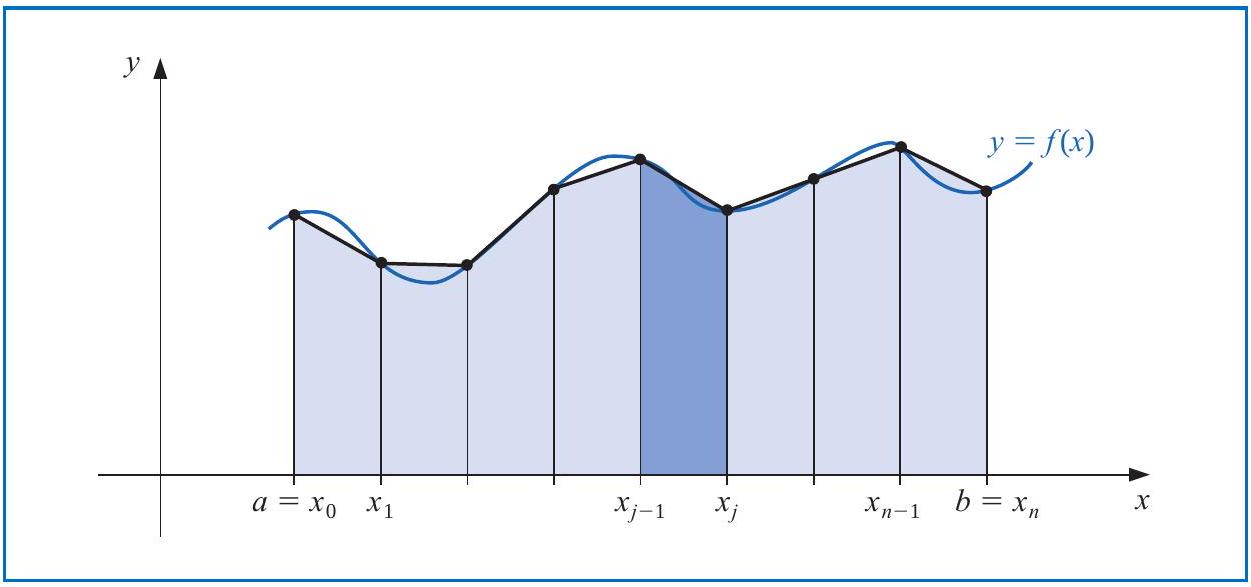
\includegraphics[width=12cm]{2025_05_15_85b7f7df47271a498e1dg-35(1)}
\caption{\scriptsize Figure $2$}
\label{fig:2025_05_15_85b7f7df47271a498e1dg-35(1)}
\end{figure}

For the Composite Midpoint rule, $n$ must again be even. (See Figure \ref{fig:2025_05_15_85b7f7df47271a498e1dg-35}.)

\begin{figure}[h]
\centering
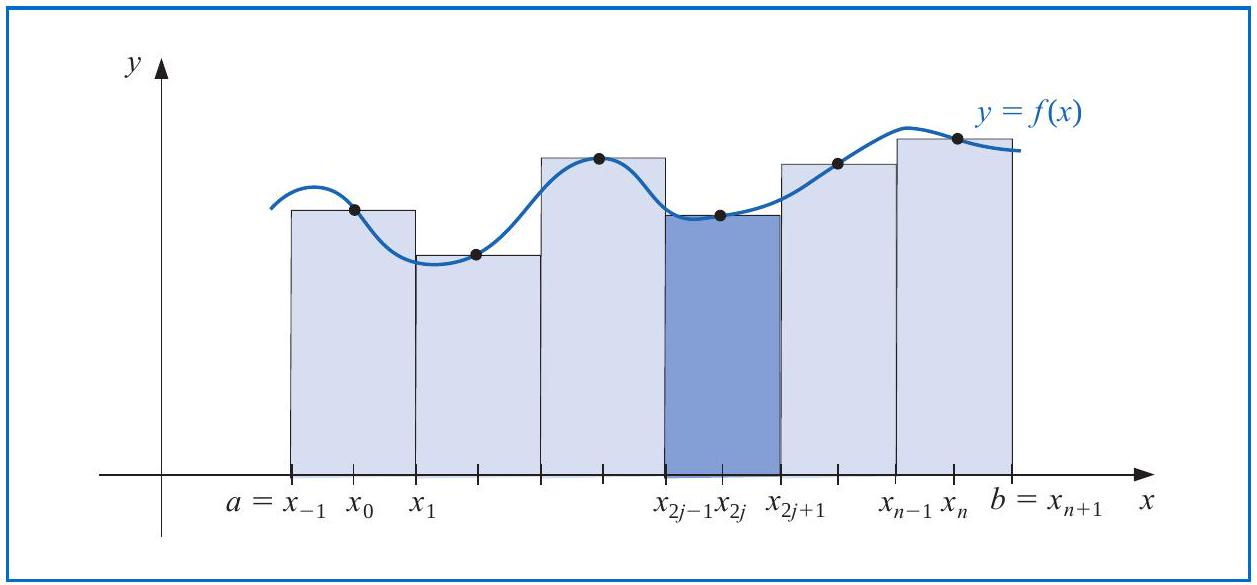
\includegraphics[width=12cm]{2025_05_15_85b7f7df47271a498e1dg-35}
\caption{\scriptsize Figure $3$}
\label{fig:2025_05_15_85b7f7df47271a498e1dg-35}
\end{figure}


\begin{theorem}
Let $f \in C^{2}[a, b], n$ be even, $h=(b-a) /(n+2)$, and $x_{j}=a+(j+1) h$ for each $j=-1,0, \ldots, n+1$. There exists a $\mu \in(a, b)$ for which the Composite Midpoint rule for $n+2$ subintervals can be written with its error term as

$$
\int_{a}^{b} f(x) d x=2 h \sum_{j=0}^{n / 2} f\left(x_{2 j}\right)+\frac{b-a}{6} h^{2} f^{\prime \prime}(\mu)
$$
\end{theorem}

\begin{example}
Determine values of $h$ that will ensure an approximation error of less than 0.00002 when approximating $\int_{0}^{\pi} \sin x d x$ and employing\\
(a) Composite Trapezoidal rule and (b) Composite Simpson's rule.
\end{example}

\begin{mysolution}
\begin{enumerate}[label=(\alph*)]
\item The error form for the Composite Trapezoidal rule for $f(x)=\sin x$ on $[0, \pi]$ is

$$
\left|\frac{\pi h^{2}}{12} f^{\prime \prime}(\mu)\right|=\left|\frac{\pi h^{2}}{12}(-\sin \mu)\right|=\frac{\pi h^{2}}{12}|\sin \mu| .
$$

To ensure sufficient accuracy with this technique we need to have

$$
\frac{\pi h^{2}}{12}|\sin \mu| \leq \frac{\pi h^{2}}{12}<0.00002
$$

Since $h=\pi / n$ implies that $n=\pi / h$, we need

$$
\frac{\pi^{3}}{12 n^{2}}<0.00002 \quad \text { which implies that } n>\left(\frac{\pi^{3}}{12(0.00002)}\right)^{1 / 2} \approx 359.44
$$

and the Composite Trapezoidal rule requires $n \geq 360$.
\item The error form for the Composite Simpson's rule for $f(x)=\sin x$ on $[0, \pi]$ is

$$
\left|\frac{\pi h^{4}}{180} f^{(4)}(\mu)\right|=\left|\frac{\pi h^{4}}{180} \sin \mu\right|=\frac{\pi h^{4}}{180}|\sin \mu| .
$$

To ensure sufficient accuracy with this technique we need to have

$$
\frac{\pi h^{4}}{180}|\sin \mu| \leq \frac{\pi h^{4}}{180}<0.00002
$$

Using again the fact that $n=\pi / h$ gives

$$
\frac{\pi^{5}}{180 n^{4}}<0.00002 \quad \text { which implies that } \quad n>\left(\frac{\pi^{5}}{180(0.00002)}\right)^{1 / 4} \approx 17.07
$$

So Composite Simpson's rule requires only $n \geq 18$.\\
Composite Simpson's rule with $n=18$ gives

$$
\int_{0}^{\pi} \sin x d x \approx \frac{\pi}{54}\left[2 \sum_{j=1}^{8} \sin \left(\frac{j \pi}{9}\right)+4 \sum_{j=1}^{9} \sin \left(\frac{(2 j-1) \pi}{18}\right)\right]=2.0000104
$$

This is accurate to within about $10^{-5}$ because the true value is $-\cos (\pi)-(-\cos (0))=2$.
\end{enumerate}\qed
\end{mysolution}

Composite Simpson's rule is the clear choice if you wish to minimize computation. For comparison purposes, consider the Composite Trapezoidal rule using $h=\pi / 18$ for the integral in Example 2. This approximation uses the same function evaluations as Composite Simpson's rule but the approximation in this case\\
$\int_{0}^{\pi} \sin x d x \approx \frac{\pi}{36}\left[2 \sum_{j=1}^{17} \sin \left(\frac{j \pi}{18}\right)+\sin 0+\sin \pi\right]=\frac{\pi}{36}\left[2 \sum_{j=1}^{17} \sin \left(\frac{j \pi}{18}\right)\right]=1.9949205$.\\
is accurate only to about $5 \times 10^{-3}$.\\
%Maple contains numerous procedures for numerical integration in the NumericalAnalysis subpackage of the Student package. First access the library as usual with\\[0pt]
%with(Student[NumericalAnalysis])\\
%The command for all methods is Quadrature with the options in the call specifying the method to be used. We will use the Trapezoidal method to illustrate the procedure. First define the function and the interval of integration with\\
%$f:=x \rightarrow \sin (x) ; a:=0.0 ; b:=\pi$
%
%Numerical integration is expected to be stable, whereas numerical differentiation is unstable.
%
%After Maple responds with the function and the interval, enter the command\\
%Quadrature $(f(x), x=$ a.. $b$, method $=$ trapezoid, partition $=20$, output $=$ value $)$\\
%1.995885973
%
%The value of the step size $h$ in this instance is the width of the interval $b-a$ divided by the number specified by partition $=20$.
%
%Simpson's method can be called in a similar manner, except that the step size $h$ is determined by $b-a$ divided by twice the value of partition. Hence, the Simpson's rule approximation using the same nodes as those in the Trapezoidal rule is called with
%
%Quadrature $(f(x), x=a . . b$, method $=$ simpson,partition $=10$, output $=$ value $)$\\
%2.000006785
%
%Any of the Newton-Cotes methods can be called using the option
%
%$$
%\text { method }=\text { newtoncotes }[\text { open }, n] \text { or } \text { method }=\text { newtoncotes }[\text { closed }, n]
%$$
%
%Be careful to correctly specify the number in partition when an even number of divisions is required, and when an open method is employed.
%
\subsection*{Round-Off Error Stability}
In Example 2 we saw that ensuring an accuracy of $2 \times 10^{-5}$ for approximating $\int_{0}^{\pi} \sin x d x$ required $360$ subdivisions of $[0, \pi]$ for the Composite Trapezoidal rule and only $18$ for Composite Simpson's rule. In addition to the fact that less computation is needed for the Simpson's technique, you might suspect that because of fewer computations this method would also involve less round-off error. However, an important property shared by all the composite integration techniques is a stability with respect to round-off error. That is, the round-off error does not depend on the number of calculations performed.

To demonstrate this rather amazing fact, suppose we apply the Composite Simpson's rule with $n$ subintervals to a function $f$ on $[a, b]$ and determine the maximum bound for the round-off error. Assume that $f\left(x_{i}\right)$ is approximated by $\tilde{f}\left(x_{i}\right)$ and that

$$
f\left(x_{i}\right)=\tilde{f}\left(x_{i}\right)+e_{i}, \quad \text { for each } i=0,1, \ldots, n,
$$

where $e_{i}$ denotes the round-off error associated with using $\tilde{f}\left(x_{i}\right)$ to approximate $f\left(x_{i}\right)$. Then the accumulated error, $e(h)$, in the Composite Simpson's rule is

$$
\begin{aligned}
e(h) & =\left|\frac{h}{3}\left[e_{0}+2 \sum_{j=1}^{(n / 2)-1} e_{2 j}+4 \sum_{j=1}^{n / 2} e_{2 j-1}+e_{n}\right]\right| \\
& \leq \frac{h}{3}\left[\left|e_{0}\right|+2 \sum_{j=1}^{(n / 2)-1}\left|e_{2 j}\right|+4 \sum_{j=1}^{n / 2}\left|e_{2 j-1}\right|+\left|e_{n}\right|\right] .
\end{aligned}
$$

If the round-off errors are uniformly bounded by $\varepsilon$, then

$$
e(h) \leq \frac{h}{3}\left[\varepsilon+2\left(\frac{n}{2}-1\right) \varepsilon+4\left(\frac{n}{2}\right) \varepsilon+\varepsilon\right]=\frac{h}{3} 3 n \varepsilon=n h \varepsilon .
$$

But $n h=b-a$, so

$$
e(h) \leq(b-a) \varepsilon
$$

a bound independent of $h$ (and $n$ ). This means that, even though we may need to divide an interval into more parts to ensure accuracy, the increased computation that is required does not increase the round-off error. This result implies that the procedure is stable as $h$ approaches zero. Recall that this was not true of the numerical differentiation procedures we have considered.

\begin{myexercise}%\label{Comprehensionquiz2}
Approximate the integral $\int_{-2}^{2} x^{3} e^{x} d x, \quad n=4$
\begin{enumerate}[label=(\alph*)]
\item Composite Trapezoidal rule with the indicated values of $n$
\item Composite Simpson's rule with the indicated values of $n$
\item Composite Midpoint rule with $n+2$ subintervals.
\end{enumerate}

\begin{mysolution}
\begin{multicols}{3}
\begin{enumerate}[label=(\alph*)]
\item $31.3653$
\item $22.47713$
\item $11.1568$
\end{enumerate}
\end{multicols}
\end{mysolution}
\end{myexercise}

\section{Romberg Integration}

\begin{youtube}
This video presents a discussion on Romberg integration. Follow the discussion and then solve the problems in the subsequent quiz.
\mylink{https://www.youtube.com/watch?v=oAh0qTJtSuk}
\end{youtube}


\begin{myexercise}%\label{Comprehensionquiz2}
Use Romberg integration to compute $R_{3,3}$ for the following integrals.
\begin{multicols}{2}
\begin{enumerate}[label=(\alph*)]
\item  $\quad \int_{1}^{1.5} x^{2} \ln x d x$\\
\item $\int_{0}^{1} x^{2} e^{-x} d x$\\
\item $\quad \int_{0}^{0.35} \frac{2}{x^{2}-4} d x$\\
\item $\quad \int_{0}^{\pi / 4} x^{2} \sin x d x$\\
\item $\quad \int_{0}^{\pi / 4} e^{3 x} \sin 2 x d x$\\
\item $\quad \int_{1}^{1.6} \frac{2 x}{x^{2}-4} d x$\\
\item $\quad \int_{3}^{3.5} \frac{x}{\sqrt{x^{2}-4}} d x$\\
\item $\int_{0}^{\pi / 4}(\cos x)^{2} d x$
\end{enumerate}
\end{multicols}
\begin{mysolution}
\begin{multicols}{2}
\begin{enumerate}[label=(\alph*)]
\item $0.1922593$ \item $0.1606105$ \item $-0.1768200$ \item $0.08875677$ \item $2.5879685$ \item $-0.7341567$ \item $0.6362135$ \item $0.6426970$
\end{enumerate}
\end{multicols}
\end{mysolution}
\end{myexercise}



\section{Adaptive Quadrature Methods}
%\activities
%Read on adaptive quadrature methods in pages \textcolor{red}{\bf page $220-227$} of the following reference and then attempt the subsequent quiz
%\begin{activity}[\cg Reading]
%\begin{enumerate}
%\item Burden, R. L., Faires, J. D., Burden, A. M. (2015). Numerical Analysis. Tenth Edition, Cengage Learning.\\
%\end{enumerate}
%\end{activity}
\activities
Read on adaptive quadrature method in the reference provided in the link below in the pages Appendix C3 and then attempt the subsequent quiz.
\begin{activity}[\cg Reading]
%\begin{enumerate}
%\item \mylink{https://math.libretexts.org/Bookshelves/Calculus/CLP-2\_Integral\_Calculus\_(Feldman\_Rechnitzer\_and\_Yeager)/04\%3A\_Appendices/4.03\%3A\_C\%3A\_More\_About\_Numerical\_Integration/4.3.01\%3A\_C.1\%3A\_Richardson\_Extrapolation}
%\end{enumerate}
\mylink{https://math.libretexts.org/Bookshelves/Calculus/\\CLP-2\_Integral\_Calculus\_(Feldman\_Rechnitzer\_and\_Yeager)}
\end{activity}
\begin{myexercise}%\label{Comprehensionquiz2}
Compute the Simpson's rule approximations $S(a, b), S(a,(a+b) / 2)$, and $S((a+b) / 2, b)$ for the following integrals, and verify the estimate given in the approximation formula.
\begin{multicols}{2}
\begin{enumerate}[label=(\alph*)]
\item $\int_1^{1.5}x^2\ln x\, dx$
\item $\int_{0}^{1} x^{2} e^{-x} d x$
\item $\int_{0}^{0.35} \frac{2}{x^{2}-4} d x$
\item $\int_{0}^{\pi / 4} x^{2} \sin x d x$
%\item $\int_{0}^{\pi / 4} e^{3 x} \sin 2 x d x$
%\item $\int_{1}^{1.6} \frac{2 x}{x^{2}-4} d x$
%\item $\int_{3}^{3.5} \frac{x}{\sqrt{x^{2}-4}} d x$
%\item $\int_{0}^{\pi / 4}(\cos x)^{2} d x$
\end{enumerate}
\end{multicols}

\begin{mysolution}
\begin{enumerate}[label=(\alph*)]
\item $S(1,1.5)=0.19224530$, $S(1,1.25)=0.039372434$, $S(1.25,1.5)=0.15288602$, and the actual value is $0.19225935$.
\item $S(0,1)=0.16240168$, $S(0,0.5)=0.028861071$, $S(0.5,1)=0.13186140$, and the actual value is $0.16060279$.
\item $S(0,0.35)=-0.17682156$, $S(0,0.175)=-0.087724382$, $S(0.175,0.35)=-0.089095736$, and the actual value is $-0.17682002$.
\item $S\left(0,\frac{\pi}{4}\right)=0.087995669$, $S\left(0,\frac{\pi}{8}\right)=0.0058315797$, $S\left(\frac{\pi}{8},\frac{\pi}{4}\right)=0.082877624$, and the actual value is $0.088755285$.
%\item $S\left(0,\frac{\pi}{4}\right)=2.5836964$, $S\left(0,\frac{\pi}{8}\right)=0.33088926$, $S\left(\frac{\pi}{8},\frac{\pi}{4}\right)=2.2568121$, and the actual value is $2.5886286$.
%\item $S(1,1.6)=-0.73910533$, $S(1,1.3)=-0.26141244$, $S(1.3,1.6)=-0.47305351$, and the actual value is $-0.73396917$.
%\item $S(3,3.5)=0.63623873$, $S(3,3.25)=0.32567095$, $S(3.25,3.5)=0.31054412$, and the actual value is $0.63621334$.
%\item $S\left(0,\frac{\pi}{4}\right)=0.64326905$, $S\left(0,\frac{\pi}{8}\right)=0.37315002$, $S\left(\frac{\pi}{8},\frac{\pi}{4}\right)=0.26958270$, and the actual value is $0.64269908$.
\end{enumerate}
\end{mysolution}
\end{myexercise}

\section{Gaussian Quadrature}
\videolesson
\begin{selfvideo}[2]
%LESSON 3: 
This video presents a discussion on Gaussian quadrature. Follow the discussion and then solve the problems in the subsequent quiz.
\end{selfvideo}
%\begin{boxB}Question: \end{boxB}

The Newton-Cotes formulas in Section $4$ of Module $4$ were derived by integrating interpolating polynomials. The error term in the interpolating polynomial of degree $n$ involves the $(n+1)$ st derivative of the function being approximated, so a Newton-Cotes formula is exact when approximating the integral of any polynomial of degree less than or equal to $n$.

All the Newton-Cotes formulas use values of the function at equally-spaced points. This restriction is convenient when the formulas are combined to form the composite rules we considered in Section $1$ of this Module, but it can significantly decrease the accuracy of the approximation. Consider, for example, the Trapezoidal rule applied to determine the integrals of the functions whose graphs are shown in Figure \ref{fig:2025_05_15_85b7f7df47271a498e1dg-57}.

%Figure 4.15\\
\begin{figure}[h]
\centering
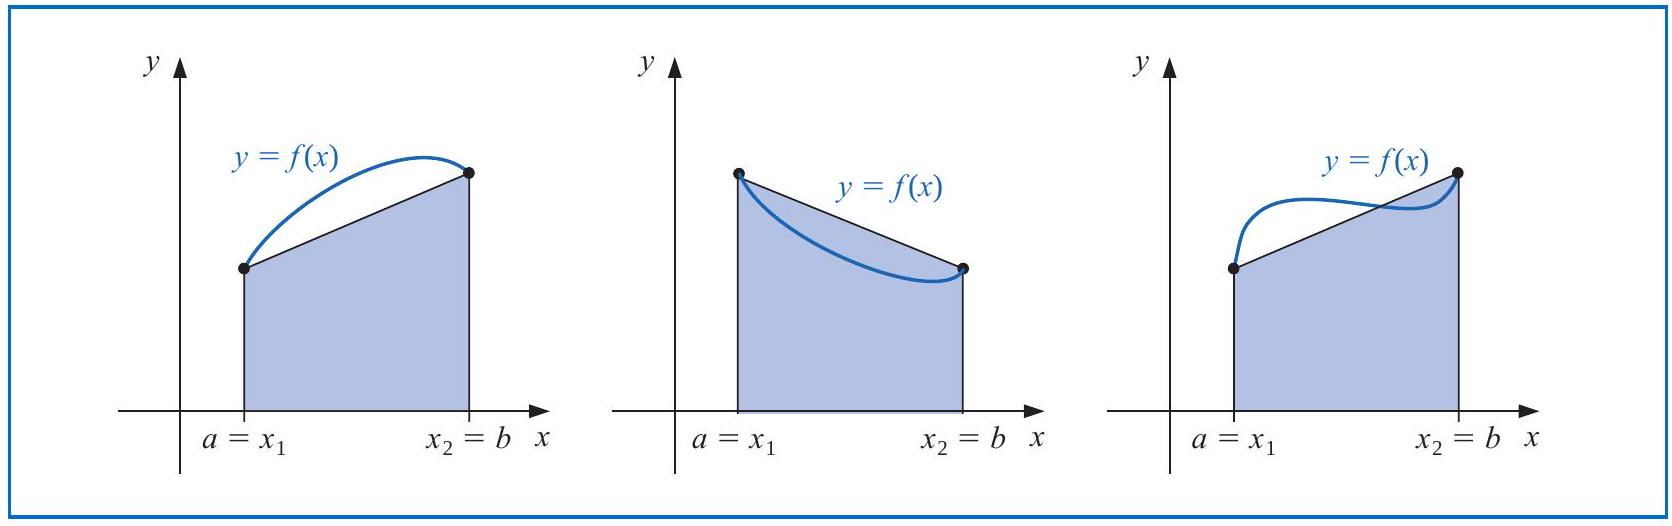
\includegraphics[width=15cm]{2025_05_15_85b7f7df47271a498e1dg-57}
\caption{\scriptsize Figure $4$}
\label{fig:2025_05_15_85b7f7df47271a498e1dg-57}
\end{figure}

The Trapezoidal rule approximates the integral of the function by integrating the linear function that joins the endpoints of the graph of the function. But this is not likely the best line for approximating the integral. Lines such as those shown in Figure \ref{fig:2025_05_15_85b7f7df47271a498e1dg-57(1)} would likely give much better approximations in most cases.

%Figure 4.16\\
\begin{figure}[h]
\centering
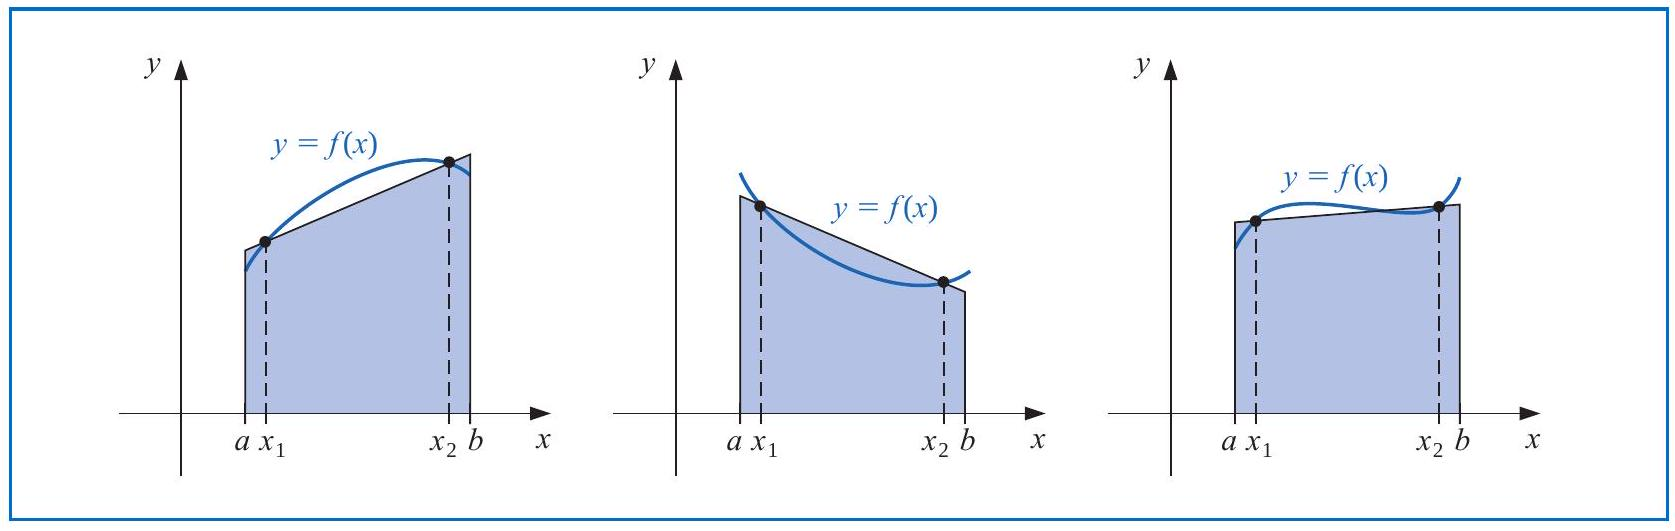
\includegraphics[width=15cm]{2025_05_15_85b7f7df47271a498e1dg-57(1)}
\caption{\scriptsize Figure $5$}
\label{fig:2025_05_15_85b7f7df47271a498e1dg-57(1)}
\end{figure}

%Gauss demonstrated his method of efficient numerical integration in a paper that was presented to the Göttingen Society in 1814. He let the nodes as well as the coefficients of the function evaluations be parameters in the summation formula and found the optimal placement of the nodes. Goldstine [Golds], pp 224-232, has an interesting description of his development.

Gaussian quadrature chooses the points for evaluation in an optimal, rather than equally spaced, way. The nodes $x_{1}, x_{2}, \ldots, x_{n}$ in the interval $[a, b]$ and coefficients $c_{1}, c_{2}, \ldots, c_{n}$, are chosen to minimize the expected error obtained in the approximation

$$
\int_{a}^{b} f(x) d x \approx \sum_{i=1}^{n} c_{i} f\left(x_{i}\right)
$$

To measure this accuracy, we assume that the best choice of these values produces the exact result for the largest class of polynomials, that is, the choice that gives the greatest degree of precision.

The coefficients $c_{1}, c_{2}, \ldots, c_{n}$ in the approximation formula are arbitrary, and the nodes $x_{1}, x_{2}, \ldots, x_{n}$ are restricted only by the fact that they must lie in $[a, b]$, the interval of integration. This gives us $2 n$ parameters to choose. If the coefficients of a polynomial are\\
considered parameters, the class of polynomials of degree at most $2 n-1$ also contains $2 n$ parameters. This, then, is the largest class of polynomials for which it is reasonable to expect a formula to be exact. With the proper choice of the values and constants, exactness on this set can be obtained.

To illustrate the procedure for choosing the appropriate parameters, we will show how to select the coefficients and nodes when $n=2$ and the interval of integration is $[-1,1]$. We will then discuss the more general situation for an arbitrary choice of nodes and coefficients and show how the technique is modified when integrating over an arbitrary interval.

Suppose we want to determine $c_{1}, c_{2}, x_{1}$, and $x_{2}$ so that the integration formula

$$
\int_{-1}^{1} f(x) d x \approx c_{1} f\left(x_{1}\right)+c_{2} f\left(x_{2}\right)
$$

gives the exact result whenever $f(x)$ is a polynomial of degree $2(2)-1=3$ or less, that is, when

$$
f(x)=a_{0}+a_{1} x+a_{2} x^{2}+a_{3} x^{3}
$$

for some collection of constants, $a_{0}, a_{1}, a_{2}$, and $a_{3}$. Because

$$
\int\left(a_{0}+a_{1} x+a_{2} x^{2}+a_{3} x^{3}\right) d x=a_{0} \int 1 d x+a_{1} \int x d x+a_{2} \int x^{2} d x+a_{3} \int x^{3} d x
$$

this is equivalent to showing that the formula gives exact results when $f(x)$ is $1, x, x^{2}$, and $x^{3}$. Hence, we need $c_{1}, c_{2}, x_{1}$, and $x_{2}$, so that

$$
\begin{array}{cc}
c_{1} \cdot 1+c_{2} \cdot 1=\int_{-1}^{1} 1 d x=2, & c_{1} \cdot x_{1}+c_{2} \cdot x_{2}=\int_{-1}^{1} x d x=0 \\
c_{1} \cdot x_{1}^{2}+c_{2} \cdot x_{2}^{2}=\int_{-1}^{1} x^{2} d x=\frac{2}{3}, & \text { and } \\
c_{1} \cdot x_{1}^{3}+c_{2} \cdot x_{2}^{3}=\int_{-1}^{1} x^{3} d x=0
\end{array}
$$

A little algebra shows that this system of equations has the unique solution

$$
c_{1}=1, \quad c_{2}=1, \quad x_{1}=-\frac{\sqrt{3}}{3}, \quad \text { and } \quad x_{2}=\frac{\sqrt{3}}{3},
$$

which gives the approximation formula


\begin{equation}\label{eqngaussquad1}
\int_{-1}^{1} f(x) d x \approx f\left(\frac{-\sqrt{3}}{3}\right)+f\left(\frac{\sqrt{3}}{3}\right) \tag{4.40}
\end{equation}


This formula has degree of precision 3, that is, it produces the exact result for every polynomial of degree 3 or less.

\subsection*{Legendre Polynomials}
The technique we have described could be used to determine the nodes and coefficients for formulas that give exact results for higher-degree polynomials, but an alternative method obtains them more easily. The set that is relevant to our problem is the Legendre polynomials, a collection $\left\{P_{0}(x), P_{1}(x), \ldots, P_{n}(x), \ldots,\right\}$ with properties:\\
\begin{enumerate}[label=(\arabic*)]
\item For each $n, P_{n}(x)$ is a monic polynomial of degree $n$.

Recall that monic polynomials have leading coefficient 1.

%Adrien-Marie Legendre (1752-1833) introduced this set of polynomials in 1785. He had numerous priority disputes with Gauss, primarily due to Gauss' failure to publish many of his original results until long after he had discovered them.
\item $\displaystyle\int_{-1}^1P(x)P_n(x)\,dx=0$ whenever $P(x)$ is a polynomial of degree less than $n$.
\end{enumerate}

The first few Legendre polynomials are
\[P_0(x)=1,\quad P_1(x)=x,\quad P_2(x)=x^2-\frac13,\]
\[P_3(x)=x^3-\frac35x,\quad\mbox{ and } \quad P_4(x)=x^4-\frac67x^2+ \frac{3}{35}.\]
 The roots of these polynomials are distinct, lie in the interval $(-1,1)$, have a symmetry with respect to the origin, and, most importantly, are the correct choice for determining the parameters that give us the nodes and coefficients for our quadrature method.

The nodes $x_1, x_2, \ldots, x_n$ needed to produce an integral approximation formula that gives exact results for any polynomial of degree less than $2n$ are the roots of the $nth-$degree Legendre polynomial. This is established by the following result.

\begin{theorem}\label{thm:Legendpolythm1}
Suppose that $x_{1}, x_{2}, \ldots, x_{n}$ are the roots of the $n$th Legendre polynomial $P_{n}(x)$ and that for each $i=1,2, \ldots, n$, the numbers $c_{i}$ are defined by

$$
c_{i}=\int_{-1}^{1} \prod_{\substack{j=1 \\ j \neq i}}^{n} \frac{x-x_{j}}{x_{i}-x_{j}} d x
$$

If $P(x)$ is any polynomial of degree less than $2 n$, then

$$
\int_{-1}^{1} P(x) d x=\sum_{i=1}^{n} c_{i} P\left(x_{i}\right)
$$
\end{theorem}
%
%Proof Let us first consider the situation for a polynomial $P(x)$ of degree less than $n$. Rewrite $P(x)$ in terms of $(n-1)$ st Lagrange coefficient polynomials with nodes at the roots of the $n$th Legendre polynomial $P_{n}(x)$. The error term for this representation involves the $n$th derivative of $P(x)$. Since $P(x)$ is of degree less than $n$, the $n$th derivative of $P(x)$ is 0 , and this representation of is exact. So
%
%$$
%P(x)=\sum_{i=1}^{n} P\left(x_{i}\right) L_{i}(x)=\sum_{i=1}^{n} \prod_{\substack{j=1 \\ j \neq i}}^{n} \frac{x-x_{j}}{x_{i}-x_{j}} P\left(x_{i}\right)
%$$
%
%and
%
%$$
%\begin{aligned}
%\int_{-1}^{1} P(x) d x & =\int_{-1}^{1}\left[\sum_{i=1}^{n} \prod_{\substack{j=1 \\
%j \neq i}}^{n} \frac{x-x_{j}}{x_{i}-x_{j}} P\left(x_{i}\right)\right] d x \\
%& =\sum_{i=1}^{n}\left[\int_{-1}^{1} \prod_{\substack{j=1 \\
%j \neq i}}^{n} \frac{x-x_{j}}{x_{i}-x_{j}} d x\right] P\left(x_{i}\right)=\sum_{i=1}^{n} c_{i} P\left(x_{i}\right)
%\end{aligned}
%$$
%
%Hence the result is true for polynomials of degree less than $n$.\\
%Now consider a polynomial $P(x)$ of degree at least $n$ but less than $2 n$. Divide $P(x)$ by the $n$th Legendre polynomial $P_{n}(x)$. This gives two polynomials $Q(x)$ and $R(x)$, each of degree less than $n$, with
%
%$$
%P(x)=Q(x) P_{n}(x)+R(x)
%$$
%
%Note that $x_{i}$ is a root of $P_{n}(x)$ for each $i=1,2, \ldots, n$, so we have
%
%$$
%P\left(x_{i}\right)=Q\left(x_{i}\right) P_{n}\left(x_{i}\right)+R\left(x_{i}\right)=R\left(x_{i}\right) .
%$$
%
%We now invoke the unique power of the Legendre polynomials. First, the degree of the polynomial $Q(x)$ is less than $n$, so (by Legendre property (2)),
%
%$$
%\int_{-1}^{1} Q(x) P_{n}(x) d x=0
%$$
%
%Then, since $R(x)$ is a polynomial of degree less than $n$, the opening argument implies that
%
%$$
%\int_{-1}^{1} R(x) d x=\sum_{i=1}^{n} c_{i} R\left(x_{i}\right)
%$$
%
%Putting these facts together verifies that the formula is exact for the polynomial $P(x)$ :
%
%$$
%\int_{-1}^{1} P(x) d x=\int_{-1}^{1}\left[Q(x) P_{n}(x)+R(x)\right] d x=\int_{-1}^{1} R(x) d x=\sum_{i=1}^{n} c_{i} R\left(x_{i}\right)=\sum_{i=1}^{n} c_{i} P\left(x_{i}\right)
%$$
%
The constants $c_{i}$ needed for the quadrature rule can be generated from the equation in Theorem \ref{thm:Legendpolythm1}, but both these constants and the roots of the Legendre polynomials are extensively tabulated. Table \ref{legendpolytable1} lists these values for $n=2,3,4$, and 5 .

%\newpage
\begin{table}[h]
\centering
\begin{tabular}{|l|l|l|}
\hline
$n$ & Roots $r_{n, i}$ & Coefficients $c_{n, i}$ \\
\hline
\multirow[t]{2}{*}{2} & 0.5773502692 & 1.0000000000 \\
\hline
 & -0.5773502692 & 1.0000000000 \\
\hline
\multirow[t]{3}{*}{3} & 0.7745966692 & 0.555555556 \\
\hline
 & 0.0000000000 & 0.888888889 \\
\hline
 & -0.7745966692 & 0.555555556 \\
\hline
\multirow[t]{4}{*}{4} & 0.8611363116 & 0.3478548451 \\
\hline
 & 0.3399810436 & 0.6521451549 \\
\hline
 & -0.3399810436 & 0.6521451549 \\
\hline
 & -0.8611363116 & 0.3478548451 \\
\hline
\multirow[t]{5}{*}{5} & 0.9061798459 & 0.2369268850 \\
\hline
 & 0.5384693101 & 0.4786286705 \\
\hline
 & 0.0000000000 & 0.5688888889 \\
\hline
 & -0.5384693101 & 0.4786286705 \\
\hline
 & -0.9061798459 & 0.2369268850 \\
\hline
\end{tabular}
\caption{\scriptsize Table $1$}
\label{legendpolytable1}
\end{table}

\begin{example}
Approximate $\int_{-1}^{1} e^{x} \cos x d x$ using Gaussian quadrature with $n=3$.
\end{example}

\begin{mysolution}
The entries in Table \ref{legendpolytable1} give us

$$
\begin{aligned}
\int_{-1}^{1} e^{x} \cos x d x \approx & 0 . \overline{5} e^{0.774596692} \cos 0.774596692 \\
& +0 . \overline{8} \cos 0+0 . \overline{5} e^{-0.774596692} \cos (-0.774596692) \\
= & 1.9333904
\end{aligned}
$$

Integration by parts can be used to show that the true value of the integral is 1.9334214 , so the absolute error is less than $3.2 \times 10^{-5}$.\qed
\end{mysolution}

\subsection*{Gaussian Quadrature on Arbitrary Intervals}
An integral $\int_{a}^{b} f(x) d x$ over an arbitrary $[a, b]$ can be transformed into an integral over $[-1,1]$ by using the change of variables (see Figure \ref{fig:2025_05_15_85b7f7df47271a498e1dg-61}):

$$
t=\frac{2 x-a-b}{b-a} \Longleftrightarrow x=\frac{1}{2}[(b-a) t+a+b]
$$


\begin{figure}
\centering
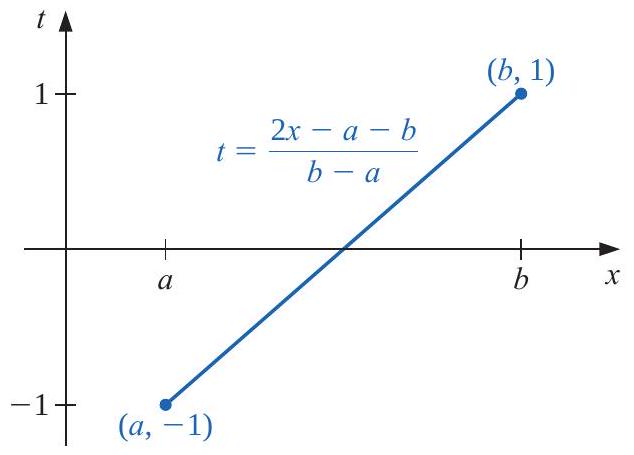
\includegraphics[width=7cm]{2025_05_15_85b7f7df47271a498e1dg-61}
\caption{\scriptsize Figure $6$}
\label{fig:2025_05_15_85b7f7df47271a498e1dg-61}
\end{figure}

This permits Gaussian quadrature to be applied to any interval $[a, b]$, because


\begin{equation}\label{eqn:Gausquad2}
\int_{a}^{b} f(x) d x=\int_{-1}^{1} f\left(\frac{(b-a) t+(b+a)}{2}\right) \frac{(b-a)}{2} d t
\end{equation}


\begin{example}
Consider the integral $\int_{1}^{3} x^{6}-x^{2} \sin (2 x) d x=317.3442466$.\\
\begin{enumerate}[label=(\alph*)]
\item Compare the results for the closed Newton-Cotes formula with $n=1$, the open Newton-Cotes formula with $n=1$, and Gaussian Quadrature when $n=2$.\\
\item Compare the results for the closed Newton-Cotes formula with $n=2$, the open Newton-Cotes formula with $n=2$, and Gaussian Quadrature when $n=3$.
\end{enumerate}
\end{example}

\begin{mysolution}
\begin{enumerate}[label=(\alph*)]
\item Each of the formulas in this part requires 2 evaluations of the function $f(x)=$ $x^{6}-x^{2} \sin (2 x)$. The Newton-Cotes approximations are

$$
\begin{aligned}
\text { Closed } n=1: & \frac{2}{2}[f(1)+f(3)]=731.6054420 \\
\text { Open } n=1: & \frac{3(2 / 3)}{2}[f(5 / 3)+f(7 / 3)]=188.7856682
\end{aligned}
$$

Gaussian quadrature applied to this problem requires that the integral first be transformed into a problem whose interval of integration is $[-1,1]$. Using Eq.\ref{eqn:Gausquad2} gives

$$
\int_{1}^{3} x^{6}-x^{2} \sin (2 x) d x=\int_{-1}^{1}(t+2)^{6}-(t+2)^{2} \sin (2(t+2)) d t
$$

Gaussian quadrature with $n=2$ then gives\\
$\int_{1}^{3} x^{6}-x^{2} \sin (2 x) d x \approx f(-0.5773502692+2)+f(0.5773502692+2)=306.8199344 ;$\\
\item Each of the formulas in this part requires 3 function evaluations. The Newton-Cotes approximations are

$$
\begin{aligned}
\text { Closed } n=2: & \frac{(1)}{3}[f(1)+4 f(2)+f(3)]=333.2380940 \\
\text { Open } n=2: & \frac{4(1 / 2)}{3}[2 f(1.5)-f(2)+2 f(2.5)]=303.5912023
\end{aligned}
$$

Gaussian quadrature with $n=3$, once the transformation has been done, gives

$$
\begin{aligned}
\int_{1}^{3} x^{6}-x^{2} \sin (2 x) d x \approx & 0 . \overline{5} f(-0.7745966692+2)+0 . \overline{8} f(2) \\
& +0 . \overline{5} f(0.7745966692+2)=317.2641516
\end{aligned}
$$

The Gaussian quadrature results are clearly superior in each instance.
\end{enumerate}
\end{mysolution}
%
%Maple has Composite Gaussian Quadrature in the NumericalAnalysis subpackage of Maple's Student package. The default for the number of partitions in the command is 10, so the results in Example 2 would be found for $n=2$ with\\
%$f:=x^{6}-x^{2} \sin (2 x) ; a:=1 ; b:=3:$\\
%Quadrature $(f(x), x=a . . b$, method $=$ gaussian $[2]$, partition $=1$, output $=$ information $)$\\
%which returns the approximation, what Maple assumes is the exact value of the integral, the absolute, and relative errors in the approximations, and the number of function evaluations.
%
%The result when $n=3$ is, of course, obtained by replacing the statement method $=$ gaussian[2] with method = gaussian [3].
\begin{myexercise}%\label{Comprehensionquiz2}
Approximate the following integrals using Gaussian quadrature with $n=2$, and compare your results to the exact values of the integrals.
\begin{multicols}{2}
\begin{enumerate}[label=(\alph*)]
\item $\int_{1}^{1.5} x^{2} \ln x d x$
\item $\int_{0}^{1} x^{2} e^{-x} d x$
\item $\int_{0}^{0.35} \frac{2}{x^{2}-4} d x$
\item $\int_{0}^{\pi / 4} x^{2} \sin x d x$
%\item $\int_{0}^{\pi / 4} e^{3 x} \sin 2 x d x$
%\item $\int_{1}^{1.6} \frac{2 x}{x^{2}-4} d x$
%\item $\int_{3}^{3.5} \frac{x}{\sqrt{x^{2}-4}} d x$
%\item $\int_{0}^{\pi / 4}(\cos x)^{2} d x$
\end{enumerate}
\end{multicols}

\begin{mysolution}
Gaussianquadraturegives:
\begin{multicols}{2}
\begin{enumerate}[label=(\alph*)]
\item $0.1922687$ \item $0.1594104$ \item $-0.1768190$ \item $0.08926302$ 
%\item $2.5913247$ \item $-0.7307230$ \item $0.6361966$ \item $0.6423172$
\end{enumerate}
\end{multicols}
\end{mysolution}
\end{myexercise}


%\discussion


\begin{posttest}[\textcolor{red}{End of Module 5 Quiz}]
\item Approximate $\int_{0}^{2} x^{2} \ln \left(x^{2}+1\right) d x$ using $h=0.25$. Use
\begin{enumerate}[label=(\alph*)]
\item Composite Trapezoidal rule.
\item Composite Simpson's rule.
\item Composite Midpoint rule.
\end{enumerate}

\item Use Romberg integration to compute $R_{4,4}$ for the following integrals.
\begin{multicols}{2}
\begin{enumerate}[label=(\alph*)]
\item  $\quad \int_{1}^{1.5} x^{2} \ln x d x$\\
\item $\int_{0}^{1} x^{2} e^{-x} d x$\\
\item $\quad \int_{0}^{0.35} \frac{2}{x^{2}-4} d x$\\
\item $\quad \int_{0}^{\pi / 4} x^{2} \sin x d x$\\
%\item $\quad \int_{0}^{\pi / 4} e^{3 x} \sin 2 x d x$\\
%\item $\quad \int_{1}^{1.6} \frac{2 x}{x^{2}-4} d x$\\
%\item $\quad \int_{3}^{3.5} \frac{x}{\sqrt{x^{2}-4}} d x$\\
%\item $\int_{0}^{\pi / 4}(\cos x)^{2} d x$
\end{enumerate}
\end{multicols}

\item Use Adaptive quadrature to approximate the following integrals to within $10^{-5}$.
\begin{multicols}{2}
\begin{enumerate}[label=(\alph*)]
\item $\int_{1}^{3} e^{2 x} \sin 3 x d x$\\
\item $\int_{1}^{3} e^{3 x} \sin 2 x d x$\\
\item $\quad \int_{0}^{5}\left(2 x \cos (2 x)-(x-2)^{2}\right) d x$\\
\item $\quad \int_{0}^{5}\left(4 x \cos (2 x)-(x-2)^{2}\right) d x$
\end{enumerate}
\end{multicols}

\item Determine constants $a, b, c$, and $d$ that will produce a quadrature formula

$$
\int_{-1}^{1} f(x) d x=a f(-1)+b f(1)+c f^{\prime}(-1)+d f^{\prime}(1)
$$

that has degree of precision $3$.
\begin{mysolution}
\begin{enumerate}[label=\arabic*.]
\item
\begin{multicols}{3}
\begin{enumerate}[label=(\alph*)]
\item $3.15947567$
\item $3.10933713$
\item $3.00906003$
\end{enumerate}
\end{multicols}

\item
\begin{multicols}{2}
\begin{enumerate}[label=(\alph*)]
\item $0.1922594$ \item $0.1606028$ \item$-0.1768200$ \item $0.08875528$ 
%\item $2.5886272$ \item $-0.7339728$ \item $0.6362134$ \item $0.6426991$
\end{enumerate}
\end{multicols}

\item Adaptive quadrature gives:
\begin{multicols}{2}
\begin{enumerate}[label=(\alph*)]
\item $108.555281$ \item $-1724.966983$  \item$-15.306308$ \item $-18.945949$
\end{enumerate}
\end{multicols}

\item $a =1$, $b =1$, $c = \frac13$, $d =-\frac13$
\end{enumerate}


\end{mysolution}
\end{posttest}

%share your understanding of properties of functions and their applications to solving rates of change problems in physical phenomenon 


%\end{actsoln}

\takehome

\comy{You are now at the last part of this module. Your  task is to do a self-reflection on your learning experience.}



\references
\begin{refenumerate}
\item Kong, Q., Siauw, T., Bayen, A., (2020). Python Programming and Numerical Methods. First Edition, Academic Press,  ISBN-13 ‏ : ‎ 978-0128195499 \\
%chapter 1 pg 7-36 functions\\
%chapter 1 pg 51-83 limits and continuity\\
%chapter 1 pg 45-50 rates of change\\
%chapter 2 pg 108-120 the derivative\\
%\item Mendelson, E. (2022). Schaum's Outline of Calculus. McGraw-Hill Education.
%chapter 6 51-55 functions
%chapter 7 59-65 limits
%chapter 8 69-74 continuity
%chapter 9 77-81 derivative
%\item Calculus \mylink{https://math.libretexts.org/Bookshelves/Calculus}
%\item Chris McMullen, 2021, Essential Calculus Skills Practice Workbook with Full Solutions, Zishka Publishing, ISBN 978-1-941691-24-3
%\item R. Adams and C. Essex, 2021, Calculus: A complete Course, Addison Wesley, ISBN 13: 978-0135732588
%\item P. Abbott and H. Neill, 2018, Calculus: A Complete Introduction: The Easy Way to Learn Calculus (Teach Yourself), ISBN 13: 978-1473678446
\end{refenumerate}





%\wrapup
%To wrap-up, answer the following questions:
%
%\begin{enumerate}
%\item 
%%when do we say that a limit of a function exists?
%%\item how do we remove discontinuity in functions?
%%\item what is the relationship between the gradient of the tangent line and the derivative?
%\end{enumerate}
















%\newpage

%\facilitation


%
\begin{center}
    {\Large \textbf{FUNCTIONS OF SEVERAL VARIABLES}}\\[2mm]
(DEFINITION, DOMAIN, RANGE, GRAPHS AND LEVEL CURVES) \\[4mm]

\mycenterbox{5 minute review}%\\[4mm]
Recap the definition of a function of several variables, and the meaning of domain, range, graph and level curves of functions of several variables.
\end{center}
\mycenterbox{Warm-up.}%\\[4mm]
\problemAnswer{
Match the function with its graph (labeled I–VI).Give reasons for your choices
\begin{multicols}{3}
\begin{enumerate}[label=(\alph*)]
\item $f(x,y)=|x|+|y|$\\[4mm]
\item $f(x,y)=|xy|$
\item $f(x,y)=\frac{1}{1+x^2+y^2}$\\2mm]
\item $f(x,y)=(x^2-y^2)^2$
\item $f(x,y)=(x-y)^2$\\[4mm]
\item $f(x,y)=\sin(|x|+|y|)$
\end{enumerate}
\end{multicols}

\begin{center}
%\centering
\includegraphics[width=10cm]{MCTutorial1Q1.JPEG}
\end{center}
%\tcbox[tcbox raise base]{Warm-up}
 
%\begin{flushright}
%\begin{tikzpicture}
%    % A body
%
%
%    % Non-rectangle shapes must be drawn as polygone
%    \begin{scope}[shift={(3,0)}]
%        \draw  (0,0.5) -- (0,4) -- (.5,4) -- (.5,4.5) -- (1.,4.5) -- (4.,4.5) --(4.,4)-- (4.5,4) --(4.5,0.5) --(4.0,0.5)--(4.0,0.0)-- (.5,0) --(0.5,0.5) -- cycle;
%        % Draw symmetry lines
%        \draw [symmetry] (.5, 0.5) -- (.5,4.0);
%        \draw [symmetry] (4, 0.5) -- (4,4.0);
%        \draw [symmetry] (.5,4.0) -- (4,4.0);
%         \draw [symmetry] (.5, 0.5) -- (4, 0.5);
%        % Dimensions
%        \draw (4.5,0) -- ++(0.5,0) coordinate (D1) -- +(5pt,0);
%        \draw (4.5,4.5) -- ++(0.5,0) coordinate (D2) -- +(5pt,0);
%        \draw [dimen] (D1) -- (D2) node {6cm};
%       
%        
%        \draw (0.0,5) -- ++(0,0.5) coordinate (D1) -- +(0,+5pt);
%        \draw (0.5,5) -- ++(0,0.5) coordinate (D2) -- +(0,+5pt);
%        \draw [dimen,-] (D1) -- (D2) node [above=5pt] {$x$ cm};
%        \draw [dimen,<-] (D1) -- ++(-5pt,0);
%        \draw [dimen,<-] (D2) -- ++(+5pt,0);
%    \end{scope}
%\end{tikzpicture}
%\end{flushright}

}


\mycenterbox{Problems.}%

%\begin{center}
%\tcbox[tcbox raise base]{ Problems. Choose from the below}
%\end{center}
\problem{Exploring functions}%
\begin{enumerate}[(a)]
\item Are the following functions even, odd, or neither? What can you say
about their range?
\begin{multicols}{4}
 \begin{enumerate}[(i)]
\item $\displaystyle \frac{3x}{x^2+2}$
\item $\displaystyle \cos x+3$
\item $\displaystyle \frac{2x^3}{\cos x+3}$
\item $\displaystyle \frac{3x^4+2x^2}{\sin x+4}$
\end{enumerate}
\end{multicols}
\item Consider the functions $\sin^n x$ and $\cos^n x$, where $n$ is a positive integer.
Which are odd, which are even, and what are their periodicities?
\item What is the periodicity of $f(x) = 2 \cos x+\sin 2x$? Is it even/odd/neither?

\end{enumerate}

\problem{Cubic functions} 
Show that $x-1$ is a factor of the cubic function%
$$P(x)=x^3-2x^2-5x+6,$$
and  find the quadratic factor $Q(x)$ such that $P(x) = (x -1)Q(x)$. Factorise
$Q(x)$ and hence sketch $P(x).$

%\newpage
\problem{Sigmoid functions*.}%
For positive integers $n$, consider the family of functions
$$\displaystyle f_n= \frac{x^n}{2^n+x^n}.$$
\begin{enumerate}[(a)]
\item What are appropriate domains and ranges for $f_n(x)$? Do they depend on $n$?

\item Is $f_n(x)$ even, odd, or neither? Does this depend on $n$?

\item Show that for $x\geq 0$, $f_n(x)$ are strictly increasing functions and that
$0\leq f_n(x) < 1.$
\item What is the value of $f_n(2)$? Does it depend on $n$?

\item By considering the values of $f_n(1.9)$ and $f_n(2.1)$ for $n = 2, 4, 8, 16, 32$ and
$64$, show that the graph of $f_n(x)$ for $x\ge 0$ is an increasing sigmoid (that
is, $S$-shaped) function that approaches a step function as $n\rightarrow \infty$.
\end{enumerate}

\mycenterbox{Selected answers and hints}%

For the warm-up, $V(x)=4x(3-x)^2$. Writing $x=1+\epsilon$, we get
$$V = 4(1 +\epsilon)(3- (1+\epsilon))^2=4(4-\epsilon^2(3-\epsilon)).$$
If $-1<\epsilon<2$ then $\epsilon^2 (3-\epsilon)\ge 0$, with equality when $\epsilon=0$. Thus the maximum
value of $V$ occurs when $\epsilon= 0$, i.e. $x = 1\rm{cm}$.

\begin{enumerate}
\item 
\begin{enumerate}[(i)]
\item Odd. The range is the interval  $[-\frac{3}{4}\sqrt{2},\; \frac{3}{4}\sqrt{2}]$
\item Even. The range is the interval $[2, 4]$.
\item Odd. The range is all of $\mathbb R$.
\item Neither. (For example, writing $\displaystyle \frac{5}{\sin x+4}$ we have $\displaystyle f(1)= \frac{5}{\sin (1)+4} \equiv 1.032 (3\rm{dp})$ which is neither $f(1)$ nor $-f(1)$.)\\[4mm]
The range is the nonnegative reals $[0,\infty)$

\end{enumerate}
\end{enumerate}











%
%\newpage
%
%\newpage
%
%
%\newtheorem{definition}[subsection]{Definition}
%\newtheorem{example}[subsection]{Example}
\newtheorem{cor}[subsection]{Corollary}
\newtheorem{pro}[subsection]{Proposition}
\newtheorem{theo}[subsection]{Theorem}
\newtheorem{lem}[subsection]{Lemma}
%\newtheorem{rem}[subsection]{Remark}

\definecolor{main}{HTML}{5989cf}    % setting main color to be used
\definecolor{sub}{HTML}{cde4ff}     % setting sub color to be used

\tcbset{
    sharp corners,
    colback = white,
    before skip = 0.2cm,    % add extra space before the box
    after skip = 0.5cm      % add extra space after the box
}                           % setting global options for tcolorbox

% You can copy any following box you like to your code.
\newtcolorbox{boxA}{
    fontupper = \bf,
    boxrule = 1.5pt,
    colframe = black % frame color
}

\newtcolorbox{boxB}{
    fontupper = \bf\color{main}, % font color
    boxrule = 1.5pt,
    colframe = main,
    rounded corners,
    arc = 5pt   % corners roundness
}
\newtcolorbox{boxC}{
    colback = sub, % background color
    boxrule = 0pt  % no borders
}

\newtcolorbox{boxD}{
    colback = sub, 
    colframe = main, 
    boxrule = 0pt, 
    toprule = 3pt, % top rule weight
    bottomrule = 3pt % bottom rule weight
}

\hypersetup{
    colorlinks=true,
    linkcolor=blue,
    filecolor=magenta,      
    urlcolor=cyan,
    pdftitle={Overleaf Example},
    pdfpagemode=FullScreen,
    }

\urlstyle{same}


\coursetitle{\mtthreeiii}{MT303}
\developers{Wyclife Rao}
\reviewers{Dr Irene Sitawa}
\modulenumber{6}
\modulename{Numerical Integration and IVP for ODEs}

% courses
\thispagestyle{empty}
\begin{tikzpicture}[overlay,remember picture,font=\sffamily\bfseries]
 \draw[ultra thick,c4,name path=big arc] ([xshift=-2mm]current page.north) arc(150:285:11) coordinate[pos=0.225] (x0);
 \begin{scope}
  \clip ([xshift=-2mm]current page.north) arc(150:285:11) --(current page.north east);
  \fill[c4!50,opacity=0.25] ([xshift=4.55cm]x0) circle (4.55);
  \fill[c4!50,opacity=0.25] ([xshift=3.4cm]x0) circle (3.4);
  \fill[c4!50,opacity=0.25] ([xshift=2.25cm]x0) circle (2.25);
  \draw[ultra thick,c4!50] (x0) arc(-90:30:6.5);
  \draw[ultra thick,c4] (x0) arc(90:-30:8.75);
  \draw[ultra thick,c4!50,name path=arc1] (x0) arc(90:-90:4.675);
  \draw[ultra thick,c4!50] (x0) arc(90:-90:2.875);
  \path[name intersections={of=big arc and arc1,by=x1}];
  \draw[ultra thick,c4,name path=arc2] (x1) arc(135:-20:4.75);
  \draw[ultra thick,c4!50] (x1) arc(135:-20:8.75);
  \path[name intersections={of=big arc and arc2,by={aux,x2}}];
  \draw[ultra thick,c4!50] (x2) arc(180:50:2.25);
 \end{scope} 
 \path[decoration={text along path,text color=c4,
                 raise = -2.8ex,
                 text  along path,
                 text = {},%|\sffamily\bfseries|02/18/2019
                 text align = center,
             },
             decorate
         ] ([xshift=-2mm]current page.north) arc(150:245:11);
 %
 \newcommand\add{4cm}
 \begin{scope}%[shift={(5,0)}]
  \path[clip,postaction={fill=c3}]
  ([xshift=2cm+\add,yshift=-8cm]current page.center) rectangle ++ (4.6,7.7);
  \draw[c5,ultra thick,fill=c2] ([xshift=0.5cm+\add,yshift=-8cm]current page.center)
   ([xshift=0.5cm+\add,yshift=-8cm]current page.center)  arc(180:60:2)
    |- ++ (-3,6) --cycle;
  \draw[ultra thick,c5] ([xshift=-1.5cm+\add,yshift=-8cm]current page.center) 
  arc(180:0:2);
  \draw[ultra thick,c5] ([xshift=0.5cm+\add,yshift=-8cm]current page.center) 
  arc(180:0:2);
  \draw[ultra thick,c5] ([xshift=2.5cm+\add,yshift=-8cm]current page.center) 
  arc(180:0:2);
  \draw[ultra thick,c5] ([xshift=4.5cm+\add,yshift=-8cm]current page.center) 
  arc(180:0:2);
  \fill[white] ([xshift=2.5cm+\add,yshift=-8cm]current page.center) +(60:2) circle(1.5mm)
  node[above
  right=0mm,text=c5!80!black]{$\rho:=\dfrac{1+\sqrt{-3}}{2}$};
 \end{scope}
 %
 \fill[c1] ([xshift=2cm+\add,yshift=-8cm]current page.center) rectangle ++ (-30.7,7.7);
 \node[text=white,anchor=west,scale=2.3,inner sep=0pt] at
 ([xshift=-10cm,yshift=-1.8cm]current page.center) {\color{ulabgold} LEARNING};
 \node[text=white,anchor=west,scale=5,inner sep=0pt] at
 ([xshift=-10cm,yshift=-3.25cm]current page.center) {MODULE \dpmdnumber};
 \node[text=white,anchor=west,scale=2.5,inner sep=0pt,text width=.4\textwidth] at
 ([xshift=-10cm,yshift=-6cm]current page.center) {\dpmdname};
 \node[text=white,anchor=east,scale=2,inner sep=0pt] at
 ([xshift=5.7cm,yshift=-7.5cm]current page.center) {\color{ulabgold}The Open University of Kenya};
 %
% \draw[gray,line width=5mm] 
% ([xshift=2mm,yshift=-1mm]current page.south west) rectangle ([xshift=-2mm,yshift=1mm]current
% page.north east);
\end{tikzpicture}

%\newpage
\pagenumbering{roman}
\thispagestyle{empty}%firstpage


\begin{center}
\vspace*{2cm}
{\Huge\bf BACHELOR OF TECHNOLOGY EDUCATION}\\[3cm]  


%{\fontsize{80}{40}\selectfont \dpcoursecode}\\[2cm]
%
%{\fontsize{30}{40} \selectfont \dpcoursename}\\[2cm]

%\rule{\textwidth}{1pt}
%\vspace{2cm}

%{\fontsize{40}{40}\selectfont \bf Module~\dpmdnumber}\\[2cm]
%
%{\fontsize{30}{40}\selectfont \bf \dpmdname}\\

\vfill
\begin{flushright}
\begin{minipage}{.6\textwidth}
\begin{tcolorbox}%[text ]
\begin{tabular}{ll}%\hline
\subtitle{Developed by:}&\displaydevelopers\\
&\\
\subtitle{Reviewed by:}&\makecell[l]{\displayreviewers}\\
\end{tabular}
\end{tcolorbox}
\end{minipage}\hspace*{-3.5cm}
\end{flushright}
\vspace*{-2.5cm}
\end{center}

\newpage
\thispagestyle{empty}
\null
\vfill
{\renewcommand\arraystretch{1.5}
\begin{tabular}{|l|l|}\hline
\subtitle{Programme Title} & Bachelor of Technology Education \\\hline
\subtitle{Course Title} & \fullcoursename\\\hline
\subtitle{Learning Module number} & Module \dpmdnumber\\\hline
\subtitle{Learning module title} & \dpmdname \\\hline
\subtitle{Module Developer} & \displaydevelopers\\\hline
\subtitle{Reviewed by} & \displayreviewers\\\hline
%\subtitle{Vision} & \vision\\\hline
%\subtitle{Audience description} & \\\hline
\end{tabular}}
\clearpage

%\section{COURSE LEARNING GUIDE}


\subsection*{Preparing for Online and Distance Learning}

This course offers you the opportunity to enter an online space where you can engage with fellow students at the university. The online forums, exercises, tasks and materials have been designed by the course facilitators in such a way that you can draw directly from their knowledge and share in their scholarly interest in online learning and assessment

We hope you will use your access to this virtual classroom to raise all your questions on the course module, to build a network great learners and to share your own thoughts and experiences to the benefit of your fellow students.

   
There are a number of steps you can take to ensure you are well prepared to make the most of this learning opportunity. This resource should prompt you to consider the following:


 \begin{enumerate}[label=\cb$\square$]
   \item How can you best prepare the space where you expect you will spend most of your time engaging in online learning (i.e. in your home or office, or even during your commute to work or whilst traveling)?
  \item   What can you do to ensure you keep working through the course material, even when you do not have Internet access?
    \item How can you familiarise yourself with the course layout, in order to be able to navigate through the steps with ease?
    \item What are the communication strategies and best practices you could consider to best engage with your fellow students and the course facilitators?
    \item What do you do when you need academic or technical support?

 \end{enumerate} 

\subsection*{General Module Guide}

The authors of this module believe that imparting knowledge should always be a mutual relationship between the students and the teachers. Students can actively construct knowledge through experiences gained in reading and answering the learning modules.

You should take time to read everything written in the module, actively and religiously solve all the exercises included to finish this course and be able to gain all the competencies and skills expected to demonstrate the learning outcomes as stated in this course. If you finish with full confidence that you understand and can apply all the knowledge you gain in this course, then you are sure to succeed in tackling the next higher subjects in your chosen course.

In this course, you will be taught not only the knowledge you need to demonstrate your learning outcomes, but you will also gain discipline, perseverance, higher thinking skills, and resourcefulness that would help strengthen your foundation to succeed in life. To successfully finish the course, you must follow the guides set forth in using this module.


\begin{description}[{format=\textcolor{ulabblue}}]
\item[STUDY ENVIRONMENT.]\leavevmode\\
Before engaging into the module, make sure that you are comfortable enough and diminish distractions. Make sure that you develop a study routine to perform and accomplish all the activities set forth by the module.
%\newpage

\item[MODE OF DELIVERY.]\leavevmode\\
Students are required to get a access a digitised copy of the module from the Virtue Learning Environment. As an open and distance learner, you should be able to learn independently and optimise the learning modes and environment available to you as much of  the delivery of all the lessons will be done asynchronously. Your success will greatly depend on your self-motivation and discipline to get your work done without your instructor to remind you from time to time.

\item[STUDY SCHEDULE.] \leavevmode\\
Remember that you have other subjects to attend to, hence, you must manage your time so that you will not be left behind in any of them. Create your own learning plan for each course to make sure that you can perform all the activities. Do not procrastinate your work, remember that time wasted can never be retrieved back. Make sure that even if you are at home, you are a student enrolled in a program, where the learning of all its courses greatly depends on your will to learn as the materials you need are all in your hands. So always be aware of your daily tasks.

\item[PRACTICE EXERCISE.]\leavevmode\\
To measure your learning from your reading, you are given practice exercises which you are supposed to answer daily. This will prepare you in performing your main task.

\item[ONLINE GROUP CHAT.]\leavevmode\\
I am going to create an online Discussion Forum and QA Forum  on the VLE.  This will serve as a room for discussion on the topics and activities found in your module.

\item[RECOMMENDED REFERENCES FOR SUPPLEMENTARY READING.]\leavevmode\\
You are given links that you need to access online. These links are online references such as e-books, online activities, and tutorial videos of the topic. These are other references you can use to further understand the topic and gain additional knowledge and skills.

\item[MAIN TASK.]\leavevmode\\
You are given a task that will require you to apply the knowledge and skills you learned from the module. This can be a group or individual activity which will measure your higher order thinking skills you acquired throughout the topic.

\item[RUBRICS. ]\leavevmode\\
This is a tool to guide you in performing your main task. Through this, you will be able to know the specific indicators that should be found in your task. This is to assess your constructive behaviour towards your learning application. You will be rated according to a 4-point scale shown below.
\begin{center}
{\color{ulabgold} \bf 4 − Excellent\quad\quad   3 −Good\quad\quad    2 − Fair \quad\quad  1 −Poor}
\end{center}
\item[REFLECTIONS.]\leavevmode\\
Writing your reflection will be a passageway to express your experiential learning in using this module. In your honest recall, write everything that you think happened to you during your learning experience in this module. Use the guide questions below:
\begin{description}[{format=\textcolor{ulabblue}}]
\item[First paragraph. ]\leavevmode\\
How was your learning experience? Maybe you can consider describing the effect of the parts of the module (sequence, discussions, examples, practice exercises, online activities, and the main task) in your learning experience. You can point out the strength and weakness of each part so that we can consider it for future improvement of this instructional material.
\item[Second paragraph.  ]\leavevmode\\
What did you learn? Did you successfully acquire the learning outcomes?

\item[Third paragraph.]\leavevmode\\
How can you use what you learned in the future?
\end{description}
\end{description}

\section{ASSESSMENT  TASKS \& EXAMINATION   RULES AND GUIDELINES}

\begin{enumerate}[label=\cb\arabic*.]
\item {\cb SUBMISSION OF ASSESSMENT TASTS.}

Since mathematical skills are best acquired through constant practice, you are encouraged to answer at least two (2) exercises a day. These practice exercises will not be graded but it will help you develop your thinking skills which will prepare you in the performance of your main tasks. You are required to submit your practice exercises every week.
\begin{center} {\cg Usually submission deadlines are set on Saturday 11:59PM EAT} \end{center}

\item  {\cb GROUP CHAT.}

You can post questions, solutions, and comment to other's post. Please be reminded that our group chat is exclusive only for discussion on topics related to this course. Everyone is required to actively participate in the discussions. Also, trolling is highly discouraged. Always observe proper online etiquettes when participating in discussions.
\begin{center} {\cb RULE OF THUMB: ALWAYS THINK BEFORE YOU CLICK} \end{center}

\item  {\cb MAIN TASK. }

Complete documentation during the preparation of your task is required to ensure that every member of the group participated and contributed in the task. May it be photos or screenshots of your virtual meetings or group works. You are going to submit it as attachment of your main task the same way as the practice exercises.



\item {\cb RECOMMENDED REFERENCES FOR SUPPLEMENTARY READING.} 

You can explore online for other references that is related to the topic to gain additional information about the topic. Do not share or post inappropriate materials online or even privately.
\end{enumerate}

\subsection*{Requirements to pass the course}

Compiled Continuous  Assignment/Activities and Tasks  with Final Performance Examination.

\subtitle{Grading System}
\begin{center}
{\renewcommand\arraystretch{1.5}
\begin{tabular}{|l|c|}\hline
Continuous Activities and Tasks  &  50\%\\\hline
Final Performance Examination. &  50\%\\\hline
\end{tabular}
}
\end{center}
%\newpage










%\subsection{INTRODUCTORY MESSAGE}

%A warm welcome to \;  \fullcoursename, {\bf Module on \dpmdname}.



%By this module learning resource, we aim to enable you  achieve the relevant competencies, depict skill, action and purpose successfully. 
 

%It has been designed to provide you with fun and meaningful opportunities for guided and independent learning at your own pace and time. You will be enabled to process the contents of the learning material while being an active learner. Your academic success lies in your own hands.  This module has the following parts and corresponding icons:





{
\renewcommand\arraystretch{4}
\begin{longtblr}{
width=\linewidth,
 colspec={ Q[1,c,f] Q[1.5,r,m] Q[4,l,m] },
%row{1} = { font=\bfseries },
% rowhead = 1,
  caption={ }, 
  label={ },
  rowsep = 4pt,
  hlines = {ulabblue!20, 1pt},
  vlines = {ulabblue!20, 1pt},
}

\includegraphics[width=2cm]{img/audience} & {\bf AUDIENCE}  &  This is a description of a target audience.   \\
{\fontsize{40}{30}\selectfont\color{ulabblue}\faCogs}& {\bf MODULE DESCRIPTION} & 
This part explains the importance of the topics discussed in the module. It will also give you a sneak peek of what you will learn and what is expected from you at the end of the module.\\

\includegraphics[width=2cm]{img/target.png} &  {\bf  EXPECTATION} & These are what you will be able to know after completing the lessons in the module\\

\includegraphics[width=2cm]{img/preactivities} & {\bf PRE-ACTIVITY} &
This activity is to get you set, activate and engage schema to learn the module. Through this activity, you will know the relevance of this activity to the topic that will be discussed in the module.\\

\includegraphics[width=2cm]{img/pretest} &  {\bf PRE - ASSESSMENT} & This will measure your prior knowledge and the concepts to be mastered throughout the lesson. \\

\includegraphics[width=1.7cm]{img/rewind} &  {\bf  RECAP} & This section will measure what learnings and skills that you understand from the previous lesson.\\

\includegraphics[width=1.5cm]{img/lesson} &  {\bf  LESSON} & This section will discuss the topic for this module.\\

\includegraphics[width=2cm]{img/activities} &  {\bf  ACTIVITIES} & This is a set of activities you will perform.\\

\includegraphics[width=2cm]{img/summary} &  {\bf  WRAP UP} & This section summarizes the concepts and applications of the lessons.\\

\includegraphics[width=2cm]{img/discussion}& {\bf DISCUSSIONS} &
This is the meat of the module. The discussion is aligned to the topic learning outcomes that is expected of you to acquire at the end of the module.\\

\includegraphics[width=1.8cm]{img/value} &  {\bf  VALUING} & This part will check the integration of values in the learning competency you will take home.\\

\includegraphics[width=1.8cm]{img/posttest} &  {\bf  POST - ASSESSMENT} & This will measure how much you have learned from the entire module.\\

\includegraphics[width=1.8cm]{img/selfreflect} & {\bf REFLECTION }
&
This part is for you to share your thoughts by writing your reflection, make sure to check your grammar and spelling to ensure the readability and so that it will not alter the thought being delivered. 
\end{longtblr}
}









%\vfill

\audience
\begin{oldactivity}{Audience Description}{
\includegraphics[width=22mm]{img/audience}}{}
This module is offered to all students taking the Bachelor of Technology Education. As an open and distance learner, you should be able to learn independently and optimise the learning modes and environment available to you. Before you begin this course, please confirm the course material, the course requirements and how the course is conducted.
\end{oldactivity}
%\newpage
\pagenumbering{arabic}



\mddescription
This module guides you into a detailed discussion of the concepts of numerical integration. Specifically you will learn about
\begin{itemize}
\item multiple integrals
\item improper integrals
\item the elementary theory of initial-value problems
\item Euler's method 
\end{itemize}
%\expectations
%\begin{objenumerate}
%
%\end{objenumerate}

\begin{mlos}
\item Identify the characteristics of multiple and improper integrals.
\item Describe numerical methods for solving multiple and improper integrals.
\item Solve first-order ODEs using Euler’s numerical method.
\item Construct numerical solutions of initial value problems.
\end{mlos}

\section{Multiple Integrals}
\videolesson
\begin{selfvideo}[1]
%LESSON 3: 
This video presents a discussion on multiple integrals. Follow the discussion and then solve the problems in the subsequent quiz.
\end{selfvideo}

The techniques discussed in the previous sections can be modified for use in the approximation of multiple integrals. Consider the double integral

$$
\iint_{R} f(x, y) d A,
$$

where $R=\{(x, y) \mid a \leq x \leq b, c \leq y \leq d\}$, for some constants $a, b, c$, and $d$, is a rectangular region in the plane. (See Figure \ref{fig:multipleintegral1}.)

%Figure 4.18\\
\begin{figure}
\centering
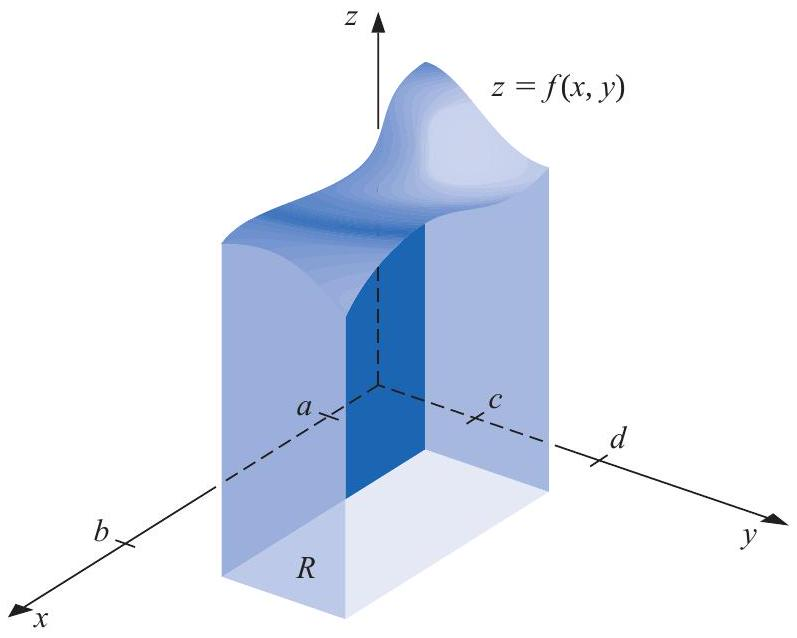
\includegraphics[width=10cm]{2025_05_15_85b7f7df47271a498e1dg-63}
\caption{\scriptsize Figure $1$}
\label{fig:multipleintegral1}
\end{figure}

The following illustration shows how the Composite Trapezoidal rule using two subintervals in each coordinate direction would be applied to this integral.

Illustration Writing the double integral as an iterated integral gives

$$
\iint_{R} f(x, y) d A=\int_{a}^{b}\left(\int_{c}^{d} f(x, y) d y\right) d x .
$$

To simplify notation, let $k=(d-c) / 2$ and $h=(b-a) / 2$. Apply the Composite Trapezoidal rule to the interior integral to obtain

$$
\int_{c}^{d} f(x, y) d y \approx \frac{k}{2}\left[f(x, c)+f(x, d)+2 f\left(x, \frac{c+d}{2}\right)\right]
$$

This approximation is of order $O\left((d-c)^{3}\right)$. Then apply the Composite Trapezoidal rule again to approximate the integral of this function of $x$ :

$$
\begin{aligned}
\int_{a}^{b}\left(\int_{c}^{d} f(x, y) d y\right) d x \approx & \int_{a}^{b}\left(\frac{d-c}{4}\right)\left[f(x, c)+2 f\left(x, \frac{c+d}{2}\right)+f(d)\right] d x \\
= & \frac{b-a}{4}\left(\frac{d-c}{4}\right)\left[f(a, c)+2 f\left(a, \frac{c+d}{2}\right)+f(a, d)\right] \\
& +\frac{b-a}{4}\left(2 ( \frac { d - c } { 4 } ) \left[f\left(\frac{a+b}{2}, c\right)\right.\right. \\
& \left.\left.+2 f\left(\frac{a+b}{2}, \frac{c+d}{2}\right)+\left(\frac{a+b}{2}, d\right)\right]\right) \\
& +\frac{b-a}{4}\left(\frac{d-c}{4}\right)\left[f(b, c)+2 f\left(b, \frac{c+d}{2}\right)+f(b, d)\right] \\
%= & \frac{(b-a)(d-c)}{16}[f(a, c)+f(a, d)+f(b, c)+f(b, d) \\
%& +2\left(f\left(\frac{a+b}{2}, c\right)+f\left(\frac{a+b}{2}, d\right)+f\left(a, \frac{c+d}{2}\right)\right. \\
%& \left.\left.+f\left(b, \frac{c+d}{2}\right)\right)+4 f\left(\frac{a+b}{2}, \frac{c+d}{2}\right)\right]
\end{aligned}
$$

Therefore
$$
\begin{aligned}
\int_{a}^{b}\left(\int_{c}^{d} f(x, y) d y\right) d x &\approx 
%\int_{a}^{b}\left(\frac{d-c}{4}\right)\left[f(x, c)+2 f\left(x, \frac{c+d}{2}\right)+f(d)\right] d x \\
%= & \frac{b-a}{4}\left(\frac{d-c}{4}\right)\left[f(a, c)+2 f\left(a, \frac{c+d}{2}\right)+f(a, d)\right] \\
%& +\frac{b-a}{4}\left(2 ( \frac { d - c } { 4 } ) \left[f\left(\frac{a+b}{2}, c\right)\right.\right. \\
%& \left.\left.+2 f\left(\frac{a+b}{2}, \frac{c+d}{2}\right)+\left(\frac{a+b}{2}, d\right)\right]\right) \\
%& +\frac{b-a}{4}\left(\frac{d-c}{4}\right)\left[f(b, c)+2 f\left(b, \frac{c+d}{2}\right)+f(b, d)\right] \\
\frac{(b-a)(d-c)}{16}[f(a, c)+f(a, d)+f(b, c)+f(b, d) \\
& +2\left(f\left(\frac{a+b}{2}, c\right)+f\left(\frac{a+b}{2}, d\right)+f\left(a, \frac{c+d}{2}\right)\right. \\
& \left.\left.+f\left(b, \frac{c+d}{2}\right)\right)+4 f\left(\frac{a+b}{2}, \frac{c+d}{2}\right)\right]
\end{aligned}
$$

This approximation is of order $O\left((b-a)(d-c)\left[(b-a)^{2}+(d-c)^{2}\right]\right)$. Figure \ref{fig:multipleintegral2} shows a grid with the number of functional evaluations at each of the nodes used in the approximation.

%Figure 4.19\\
\begin{figure}[h]
\centering
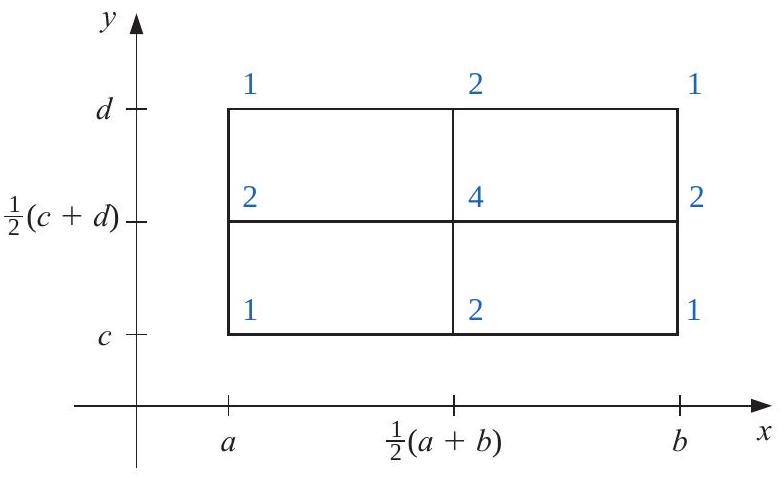
\includegraphics[width=10cm]{2025_05_15_85b7f7df47271a498e1dg-64}
\caption{\scriptsize Figure $2$}
\label{fig:multipleintegral2}
\end{figure}

As the illustration shows, the procedure is quite straightforward. But the number of function evaluations grows with the square of the number required for a single integral. In a practical situation we would not expect to use a method as elementary as the Composite Trapezoidal rule. Instead we will employ the Composite Simpson's rule to illustrate the general approximation technique, although any other composite formula could be used in its place.

To apply the Composite Simpson's rule, we divide the region $R$ by partitioning both $[a, b]$ and $[c, d]$ into an even number of subintervals. To simplify the notation, we choose even integers $n$ and $m$ and partition $[a, b]$ and $[c, d]$ with the evenly spaced mesh points $x_{0}, x_{1}, \ldots, x_{n}$ and $y_{0}, y_{1}, \ldots, y_{m}$, respectively. These subdivisions determine step sizes $h=$ $(b-a) / n$ and $k=(d-c) / m$. Writing the double integral as the iterated integral

$$
\iint_{R} f(x, y) d A=\int_{a}^{b}\left(\int_{c}^{d} f(x, y) d y\right) d x
$$

we first use the Composite Simpson's rule to approximate

$$
\int_{c}^{d} f(x, y) d y
$$

treating $x$ as a constant.

Let $y_{j}=c+j k$, for each $j=0,1, \ldots, m$. Then

$$
\begin{aligned}
\int_{c}^{d} f(x, y) d y= & \frac{k}{3}\left[f\left(x, y_{0}\right)+2 \sum_{j=1}^{(m / 2)-1} f\left(x, y_{2 j}\right)+4 \sum_{j=1}^{m / 2} f\left(x, y_{2 j-1}\right)+f\left(x, y_{m}\right)\right] \\
& -\frac{(d-c) k^{4}}{180} \frac{\partial^{4} f}{\partial y^{4}}(x, \mu)
\end{aligned}
$$

for some $\mu$ in ( $c, d$ ). Thus

$$
\begin{aligned}
\int_{a}^{b} \int_{c}^{d} f(x, y) d y d x= & \frac{k}{3}\left[\int_{a}^{b} f\left(x, y_{0}\right) d x+2 \sum_{j=1}^{(m / 2)-1} \int_{a}^{b} f\left(x, y_{2 j}\right) d x\right. \\
& \left.+4 \sum_{j=1}^{m / 2} \int_{a}^{b} f\left(x, y_{2 j-1}\right) d x+\int_{a}^{b} f\left(x, y_{m}\right) d x\right] \\
& -\frac{(d-c) k^{4}}{180} \int_{a}^{b} \frac{\partial^{4} f}{\partial y^{4}}(x, \mu) d x
\end{aligned}
$$

Composite Simpson's rule is now employed on the integrals in this equation. Let $x_{i}=a+i h$, for each $i=0,1, \ldots, n$. Then for each $j=0,1, \ldots, m$, we have

$$
\begin{aligned}
\int_{a}^{b} f\left(x, y_{j}\right) d x= & \frac{h}{3}\left[f\left(x_{0}, y_{j}\right)+2 \sum_{i=1}^{(n / 2)-1} f\left(x_{2 i}, y_{j}\right)+4 \sum_{i=1}^{n / 2} f\left(x_{2 i-1}, y_{j}\right)+f\left(x_{n}, y_{j}\right)\right] \\
& -\frac{(b-a) h^{4}}{180} \frac{\partial^{4} f}{\partial x^{4}}\left(\xi_{j}, y_{j}\right)
\end{aligned}
$$

for some $\xi_{j}$ in ( $a, b$ ). The resulting approximation has the form

$$
\begin{aligned}
\int_{a}^{b} \int_{c}^{d} f(x, y) d y d x \approx & \frac{h k}{9}\left\{\left[f\left(x_{0}, y_{0}\right)+2 \sum_{i=1}^{(n / 2)-1} f\left(x_{2 i}, y_{0}\right)+4 \sum_{i=1}^{n / 2} f\left(x_{2 i-1}, y_{0}\right)+f\left(x_{n}, y_{0}\right)\right]\right. \\
& +2\left[\sum_{j=1}^{(m / 2)-1} f\left(x_{0}, y_{2 j}\right)+2 \sum_{j=1}^{(m / 2)-1} \sum_{i=1}^{(n / 2)-1} f\left(x_{2 i}, y_{2 j}\right)\right. \\
& \left.+4 \sum_{j=1}^{(m / 2)-1} \sum_{i=1}^{n / 2} f\left(x_{2 i-1}, y_{2 j}\right)+\sum_{j=1}^{(m / 2)-1} f\left(x_{n}, y_{2 j}\right)\right] \\
& +4\left[\sum_{j=1}^{m / 2} f\left(x_{0}, y_{2 j-1}\right)+2 \sum_{j=1}^{m / 2} \sum_{i=1}^{(n / 2)-1} f\left(x_{2 i}, y_{2 j-1}\right)\right. \\
& \left.+4 \sum_{j=1}^{m / 2} \sum_{i=1}^{n / 2} f\left(x_{2 i-1}, y_{2 j-1}\right)+\sum_{j=1}^{m / 2} f\left(x_{n}, y_{2 j-1}\right)\right] \\
& \left.+\left[f\left(x_{0}, y_{m}\right)+2 \sum_{i=1}^{(n / 2)-1} f\left(x_{2 i}, y_{m}\right)+4 \sum_{i=1}^{n / 2} f\left(x_{2 i-1}, y_{m}\right)+f\left(x_{n}, y_{m}\right)\right]\right\}
\end{aligned}
$$

The error term $E$ is given by

$$
\begin{aligned}
E= & \frac{-k(b-a) h^{4}}{540}\left[\frac{\partial^{4} f}{\partial x^{4}}\left(\xi_{0}, y_{0}\right)+2 \sum_{j=1}^{(m / 2)-1} \frac{\partial^{4} f}{\partial x^{4}}\left(\xi_{2 j}, y_{2 j}\right)+4 \sum_{j=1}^{m / 2} \frac{\partial^{4} f}{\partial x^{4}}\left(\xi_{2 j-1}, y_{2 j-1}\right)\right. \\
& \left.+\frac{\partial^{4} f}{\partial x^{4}}\left(\xi_{m}, y_{m}\right)\right]-\frac{(d-c) k^{4}}{180} \int_{a}^{b} \frac{\partial^{4} f}{\partial y^{4}}(x, \mu) d x
\end{aligned}
$$

If $\partial^{4} f / \partial x^{4}$ is continuous, the Intermediate Value Theorem can be repeatedly applied to show that the evaluation of the partial derivatives with respect to $x$ can be replaced by a common value and that

$$
E=\frac{-k(b-a) h^{4}}{540}\left[3 m \frac{\partial^{4} f}{\partial x^{4}}(\bar{\eta}, \bar{\mu})\right]-\frac{(d-c) k^{4}}{180} \int_{a}^{b} \frac{\partial^{4} f}{\partial y^{4}}(x, \mu) d x
$$

for some $(\bar{\eta}, \bar{\mu})$ in $R$. If $\partial^{4} f / \partial y^{4}$ is also continuous, the Weighted Mean Value Theorem for Integrals implies that

$$
\int_{a}^{b} \frac{\partial^{4} f}{\partial y^{4}}(x, \mu) d x=(b-a) \frac{\partial^{4} f}{\partial y^{4}}(\hat{\eta}, \hat{\mu})
$$

for some ( $\hat{\eta}, \hat{\mu}$ ) in $R$. Because $m=(d-c) / k$, the error term has the form

$$
E=\frac{-k(b-a) h^{4}}{540}\left[3 m \frac{\partial^{4} f}{\partial x^{4}}(\bar{\eta}, \bar{\mu})\right]-\frac{(d-c)(b-a)}{180} k^{4} \frac{\partial^{4} f}{\partial y^{4}}(\hat{\eta}, \hat{\mu})
$$

which simplifies to

$$
E=-\frac{(d-c)(b-a)}{180}\left[h^{4} \frac{\partial^{4} f}{\partial x^{4}}(\bar{\eta}, \bar{\mu})+k^{4} \frac{\partial^{4} f}{\partial y^{4}}(\hat{\eta}, \hat{\mu})\right]
$$

for some $(\bar{\eta}, \bar{\mu})$ and $(\hat{\eta}, \hat{\mu})$ in $R$.

\begin{example}\label{examp:multipleintegral1}
Use Composite Simpson's rule with $n=4$ and $m=2$ to approximate

$$
\int_{1.4}^{2.0} \int_{1.0}^{1.5} \ln (x+2 y) d y d x
$$
\end{example}

\begin{mysolution}
The step sizes for this application are $h=(2.0-1.4) / 4=0.15$ and $k=$ $(1.5-1.0) / 2=0.25$. The region of integration $R$ is shown in Figure 4.20, together with the nodes $\left(x_{i}, y_{j}\right)$, where $i=0,1,2,3,4$ and $j=0,1,2$. It also shows the coefficients $w_{i, j}$ of $f\left(x_{i}, y_{i}\right)=\ln \left(x_{i}+2 y_{i}\right)$ in the sum that gives the Composite Simpson's rule approximation to the integral.

\begin{center}
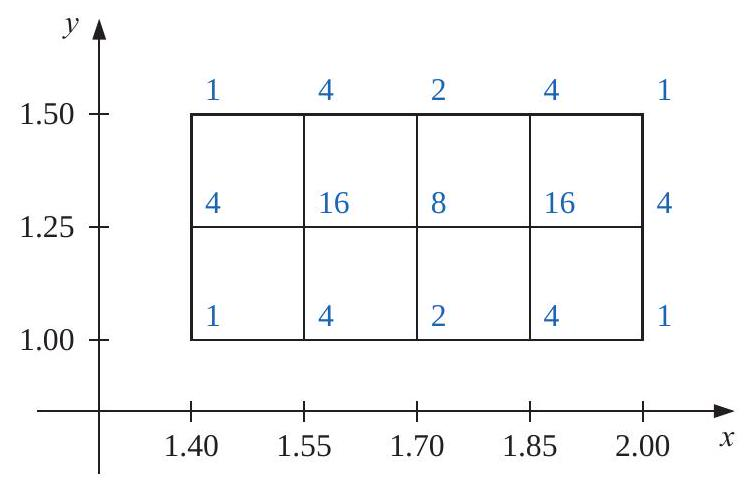
\includegraphics[width=10cm]{2025_05_15_85b7f7df47271a498e1dg-67}
\end{center}

The approximation is

$$
\begin{aligned}
\int_{1.4}^{2.0} \int_{1.0}^{1.5} \ln (x+2 y) d y d x & \approx \frac{(0.15)(0.25)}{9} \sum_{i=0}^{4} \sum_{j=0}^{2} w_{i, j} \ln \left(x_{i}+2 y_{j}\right) \\
& =0.4295524387
\end{aligned}
$$

We have

$$
\frac{\partial^{4} f}{\partial x^{4}}(x, y)=\frac{-6}{(x+2 y)^{4}} \quad \text { and } \quad \frac{\partial^{4} f}{\partial y^{4}}(x, y)=\frac{-96}{(x+2 y)^{4}}
$$

and the maximum values of the absolute values of these partial derivatives occur on $R$ when $x=1.4$ and $y=1.0$. So the error is bounded by

$$
|E| \leq \frac{(0.5)(0.6)}{180}\left[(0.15)^{4} \max _{(x, y) \operatorname{in} R} \frac{6}{(x+2 y)^{4}}+(0.25)^{4} \max _{(x, y) \operatorname{in} R} \frac{96}{(x+2 y)^{4}}\right] \leq 4.72 \times 10^{-6}
$$

The actual value of the integral to ten decimal places is

$$
\int_{1.4}^{2.0} \int_{1.0}^{1.5} \ln (x+2 y) d y d x=0.4295545265
$$

so the approximation is accurate to within $2.1 \times 10^{-6}$\qed
\end{mysolution}

The same techniques can be applied for the approximation of triple integrals as well as higher integrals for functions of more than three variables. The number of functional evaluations required for the approximation is the product of the number of functional evaluations required when the method is applied to each variable.

\subsection*{Gaussian Quadrature for Double Integral Approximation}
To reduce the number of functional evaluations, more efficient methods such as Gaussian quadrature, Romberg integration, or Adaptive quadrature can be incorporated in place of the Newton-Cotes formulas. The following example illustrates the use of Gaussian quadrature for the integral considered in Example 1.

\begin{example}
Use Gaussian quadrature with $n=3$ in both dimensions to approximate the integral

$$
\int_{1.4}^{2.0} \int_{1.0}^{1.5} \ln (x+2 y) d y d x
$$
\end{example}

\begin{mysolution}
Before employing Gaussian quadrature to approximate this integral, we need to transform the region of integration

$$
R=\{(x, y) \mid 1.4 \leq x \leq 2.0,1.0 \leq y \leq 1.5\}
$$

into

$$
\hat{R}=\{(u, v) \mid-1 \leq u \leq 1,-1 \leq v \leq 1\} .
$$

The linear transformations that accomplish this are

$$
u=\frac{1}{2.0-1.4}(2 x-1.4-2.0) \quad \text { and } \quad v=\frac{1}{1.5-1.0}(2 y-1.0-1.5),
$$

or, equivalently, $x=0.3 u+1.7$ and $y=0.25 v+1.25$. Employing this change of variables gives an integral on which Gaussian quadrature can be applied:

$$
\int_{1.4}^{2.0} \int_{1.0}^{1.5} \ln (x+2 y) d y d x=0.075 \int_{-1}^{1} \int_{-1}^{1} \ln (0.3 u+0.5 v+4.2) d v d u
$$

The Gaussian quadrature formula for $n=3$ in both $u$ and $v$ requires that we use the nodes

$$
u_{1}=v_{1}=r_{3,2}=0, \quad u_{0}=v_{0}=r_{3,1}=-0.7745966692,
$$

and

$$
u_{2}=v_{2}=r_{3,3}=0.7745966692
$$

The associated weights are $c_{3,2}=0 . \overline{8}$ and $c_{3,1}=c_{3,3}=0 . \overline{5}$. (These are given in Table 4.12 on page 232.) The resulting approximation is

$$
\begin{aligned}
\int_{1.4}^{2.0} \int_{1.0}^{1.5} \ln (x+2 y) d y d x & \approx 0.075 \sum_{i=1}^{3} \sum_{j=1}^{3} c_{3, i} c_{3, j} \ln \left(0.3 r_{3, i}+0.5 r_{3, j}+4.2\right) \\
& =0.4295545313
\end{aligned}
$$

Although this result requires only $9$ functional evaluations compared to $15$ for the Composite Simpson's rule considered in Example \ref{examp:multipleintegral1}, it is accurate to within $4.8 \times 10^{-9}$, compared to $2.1 \times 10^{-6}$ accuracy in Example \ref{examp:multipleintegral1}.\qed
\end{mysolution}

\subsection*{Non-Rectangular Regions}
The use of approximation methods for double integrals is not limited to integrals with rectangular regions of integration. The techniques previously discussed can be modified to approximate double integrals of the form


\begin{equation}\label{eqn:nonrectangle1}
\int_{a}^{b} \int_{c(x)}^{d(x)} f(x, y) d y d x \tag{4.42}
\end{equation}


or


\begin{equation}\label{eqn:nonrectangle2}
\int_{c}^{d} \int_{a(y)}^{b(y)} f(x, y) d x d y . \tag{4.43}
\end{equation}


In fact, integrals on regions not of this type can also be approximated by performing appropriate partitions of the region. (See Exercise 10.)

To describe the technique involved with approximating an integral in the form

$$
\int_{a}^{b} \int_{c(x)}^{d(x)} f(x, y) d y d x
$$

we will use the basic Simpson's rule to integrate with respect to both variables. The step size for the variable $x$ is $h=(b-a) / 2$, but the step size for $y$ varies with $x$ (see Figure 4.21) and is written

$$
k(x)=\frac{d(x)-c(x)}{2} .
$$

%Figure 4.21\\
\begin{figure}[h]
\centering
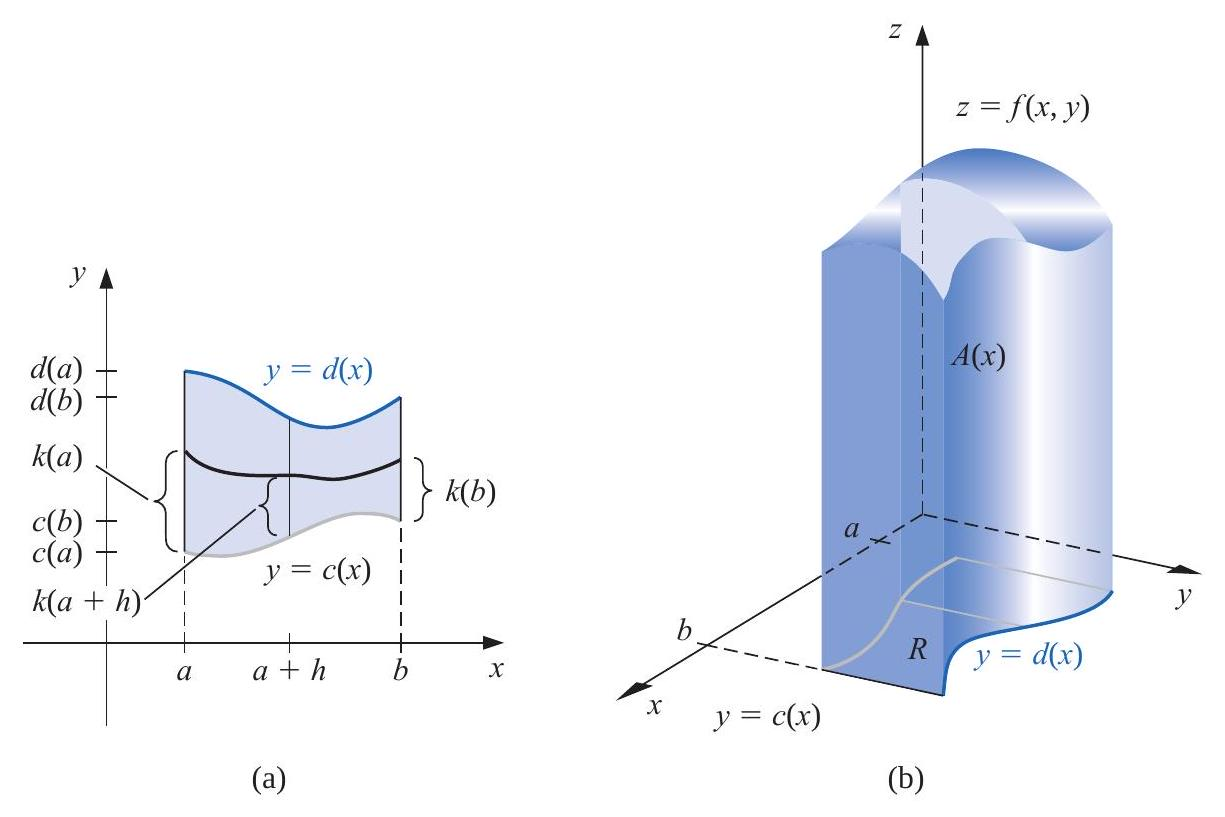
\includegraphics[width=13cm]{2025_05_15_85b7f7df47271a498e1dg-69}
\caption{\scriptsize Figure $3$: Non-rectangular region}
\label{fig:nonrectangle1}
\end{figure}

This gives

$$
\begin{aligned}
\int_{a}^{b} \int_{c(x)}^{d(x)} f(x, y) d y d x \approx & \int_{a}^{b} \frac{k(x)}{3}[f(x, c(x))+4 f(x, c(x)+k(x))+f(x, d(x))] d x \\
\approx & \frac{h}{3}\left\{\frac{k(a)}{3}[f(a, c(a))+4 f(a, c(a)+k(a))+f(a, d(a))]\right. \\
& +\frac{4 k(a+h)}{3}[f(a+h, c(a+h))+4 f(a+h, c(a+h) \\
& +k(a+h))+f(a+h, d(a+h))] \\
& \left.+\frac{k(b)}{3}[f(b, c(b))+4 f(b, c(b)+k(b))+f(b, d(b))]\right\}
\end{aligned}
$$

%Algorithm 4.4 applies the Composite Simpson's rule to an integral in the form (4.42). Integrals in the form (4.43) can, of course, be handled similarly.
%
%\section*{Simpson's Double Integral}
%To approximate the integral
%
%$$
%I=\int_{a}^{b} \int_{c(x)}^{d(x)} f(x, y) d y d x
%$$
%
%INPUT endpoints $a, b$ : even positive integers $m, n$.\\
%OUTPUT approximation $J$ to $I$.\\
%Step 1 Set $h=(b-a) / n$;\\
%$J_{1}=0 ; \quad($ End terms.$)$\\
%$J_{2}=0 ; \quad$ (Even terms.)\\
%$J_{3}=0 . \quad$ (Odd terms.)\\
%Step 2 For $i=0,1, \ldots, n$ do Steps 3-8.\\
%Step 3 Set $x=a+i h$; (Composite Simpson's method for $x$.)
%
%$$
%\begin{aligned}
%& H X=(d(x)-c(x)) / m ; \\
%& K_{1}=f(x, c(x))+f(x, d(x)) ; \quad(\text { End terms } .) \\
%& K_{2}=0 ; \quad(\text { Even terms } .) \\
%& K_{3}=0 . \quad(\text { Odd terms } .)
%\end{aligned}
%$$
%
%Step 4 For $j=1,2, \ldots, m-1$ do Step 5 and 6.\\
%Step 5 Set $y=c(x)+j H X$;
%
%$$
%Q=f(x, y)
%$$
%
%Step 6 If $j$ is even then set $K_{2}=K_{2}+Q$ else set $K_{3}=K_{3}+Q$.
%
%Step 7 Set $L=\left(K_{1}+2 K_{2}+4 K_{3}\right) H X / 3$.\\
%$\left(L \approx \int_{c\left(x_{i}\right)}^{d\left(x_{i}\right)} f\left(x_{i}, y\right) d y\right.$ by the Composite Simpson's method.)\\
%Step 8 If $i=0$ or $i=n$ then set $J_{1}=J_{1}+L$ else if $i$ is even then set $J_{2}=J_{2}+L$ else set $J_{3}=J_{3}+L$.
%
%The reduced calculation makes it generally worthwhile to apply\\
%Gaussian quadrature rather than a Simpson's technique when approximating double integrals.
%
%Step 9 Set $J=h\left(J_{1}+2 J_{2}+4 J_{3}\right) / 3$.\\
%Step 10 OUTPUT (J); STOP.
%
To apply Gaussian quadrature to the double integral

$$
\int_{a}^{b} \int_{c(x)}^{d(x)} f(x, y) d y d x
$$

first requires transforming, for each $x$ in $[a, b]$, the variable $y$ in the interval $[c(x), d(x)]$ into the variable $t$ in the interval $[-1,1]$. This linear transformation gives

$$
f(x, y)=f\left(x, \frac{(d(x)-c(x)) t+d(x)+c(x)}{2}\right) \quad \text { and } \quad d y=\frac{d(x)-c(x)}{2} d t .
$$

Then, for each $x$ in $[a, b]$, we apply Gaussian quadrature to the resulting integral

$$
\int_{c(x)}^{d(x)} f(x, y) d y=\int_{-1}^{1} f\left(x, \frac{(d(x)-c(x)) t+d(x)+c(x)}{2}\right) d t
$$

to produce

$$
\int_{a}^{b} \int_{c(x)}^{d(x)} f(x, y) d y d x \approx \int_{a}^{b} \frac{d(x)-c(x)}{2} \sum_{j=1}^{n} c_{n, j} f\left(x, \frac{(d(x)-c(x)) r_{n, j}+d(x)+c(x)}{2}\right) d x
$$

where, as before, the roots $r_{n, j}$ and coefficients $c_{n, j}$ come from Table $1$ oModule $5$. Now the interval $[a, b]$ is transformed to $[-1,1]$, and Gaussian quadrature is applied to approximate the integral on the right side of this equation. 
%The details are given in Algorithm 4.5.

%\section*{Gaussian Double Integral}
%To approximate the integral
%
%$$
%\int_{a}^{b} \int_{c(x)}^{d(x)} f(x, y) d y d x:
%$$
%
%INPUT endpoints $a, b$; positive integers $m, n$.\\
%(The roots $r_{i, j}$ and coefficients $c_{i, j}$ need to be available for $i=\max \{m, n\}$ and for $1 \leq j \leq i$.)
%
%OUTPUT approximation $J$ to $I$.\\
%Step 1 Set $h_{1}=(b-a) / 2$;
%
%$$
%\begin{aligned}
%& h_{2}=(b+a) / 2 \\
%& J=0
%\end{aligned}
%$$
%
%Step 2 For $i=1,2, \ldots, m$ do Steps 3-5.\\
%Step 3 Set $J X=0$;
%
%$$
%\begin{aligned}
%& x=h_{1} r_{m, i}+h_{2} ; \\
%& d_{1}=d(x) ; \\
%& c_{1}=c(x) ; \\
%& k_{1}=\left(d_{1}-c_{1}\right) / 2 ; \\
%& k_{2}=\left(d_{1}+c_{1}\right) / 2 .
%\end{aligned}
%$$
%
%\begin{center}
%\includegraphics[max width=\textwidth]{2025_05_15_85b7f7df47271a498e1dg-72}
%\end{center}
%
%Step 4 For $j=1,2, \ldots, n$ do
%
%$$
%\begin{aligned}
%& \text { set } y=k_{1} r_{n, j}+k_{2} \\
%& \quad Q=f(x, y) \\
%& \quad J X=J X+c_{n, j} Q
%\end{aligned}
%$$
%
%Step 5 Set $J=J+c_{m, i} k_{1} J X$.\\
%Step 6 Set $J=h_{1} J$.\\
%Step 7 OUTPUT ( $J$ );\\
%STOP.
%
\begin{boxB}
\underline{Illustration}
The volume of the solid in Figure \ref{fig:multipleintegralill1} is approximated by applying Simpson's Double Integral Algorithm with $n=m=10$ to

$$
\int_{0.1}^{0.5} \int_{x^{3}}^{x^{2}} e^{y / x} d y d x
$$

This requires $121$ evaluations of the function $f(x, y)=e^{y / x}$ and produces the value $0.0333054$, which approximates the volume of the solid shown in Figure \ref{fig:multipleintegralill1} to nearly seven decimal places. Applying the Gaussian Quadrature Algorithm with $n=m=5$ requires only $25$ function evaluations and gives the approximation $0.03330556611$, which is accurate to $11$ decimal places.
\end{boxB}
%Figure 4.22\\
\begin{figure}[h]
\centering
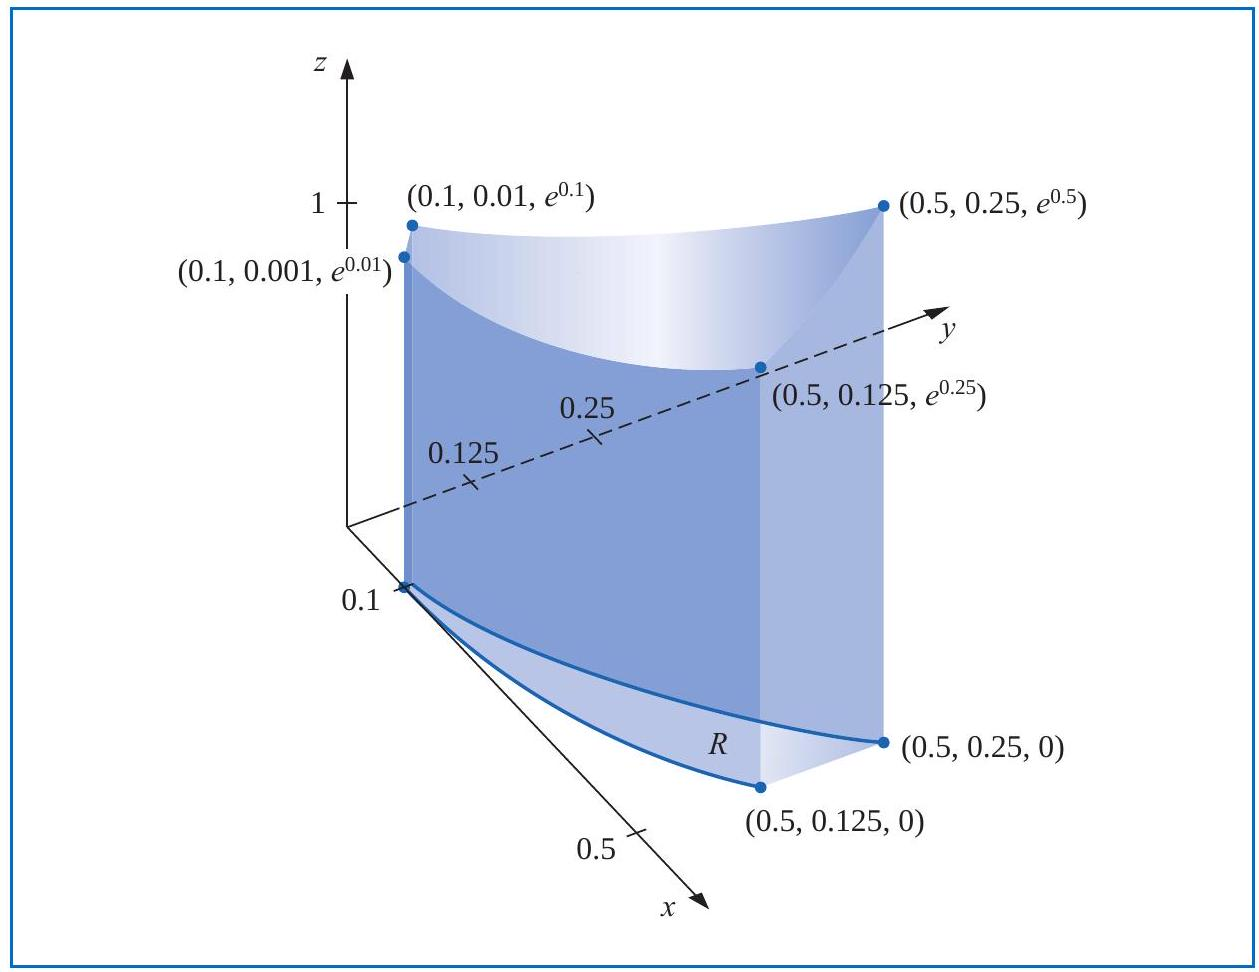
\includegraphics[width=10cm]{2025_05_15_85b7f7df47271a498e1dg-72(1)}
\caption{\scriptsize Figure $4$}
\label{fig:multipleintegralill1}
\end{figure}
%
%The reduced calculation makes it almost always worthwhile to apply Gaussian quadrature rather than a Simpson's technique when approximating triple or higher integrals.
%
\subsection*{Triple Integral Approximation}
Triple integrals of the form

$$
\int_{a}^{b} \int_{c(x)}^{d(x)} \int_{\alpha(x, y)}^{\beta(x, y)} f(x, y, z) d z d y d x
$$

(see Figure \ref{fig:tripleintegrlas1}) are approximated in a similar manner. Because of the number of calculations involved, Gaussian quadrature is the method of choice. 

\begin{figure}[h]
\centering
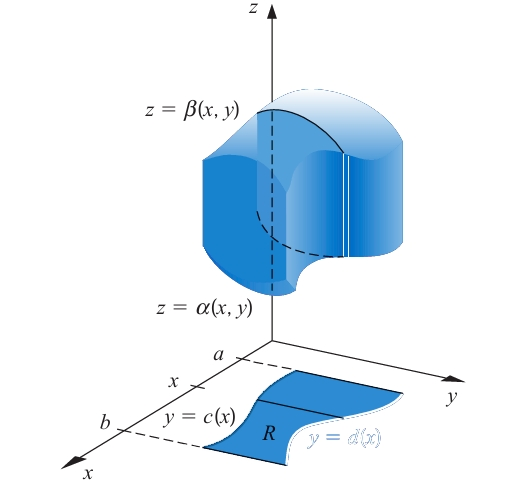
\includegraphics[width=10cm]{tripleintegrlas1}
\caption{\scriptsize Figure $5$}
\label{fig:tripleintegrlas1}
\end{figure}

%Figure 4.23
%
%\section*{Gaussian Triple Integral}
%To approximate the integral
%
%$$
%\int_{a}^{b} \int_{c(x)}^{d(x)} \int_{\alpha(x, y)}^{\beta(x, y)} f(x, y, z) d z d y d x
%$$
%
%INPUT endpoints $a, b$; positive integers $m, n, p$.\\
%(The roots $r_{i, j}$ and coefficients $c_{i, j}$ need to be available for $i=\max \{n, m, p\}$ and for $1 \leq j \leq i$.)
%
%\section*{OUTPUT approximation $J$ to $I$.}
%Step 1 Set $h_{1}=(b-a) / 2$;
%
%$$
%\begin{aligned}
%& h_{2}=(b+a) / 2 ; \\
%& J=0 .
%\end{aligned}
%$$
%
%Step 2 For $i=1,2, \ldots, m$ do Steps 3-8.\\
%\includegraphics[max width=\textwidth, center]{2025_05_15_85b7f7df47271a498e1dg-74}
%
%Step 3 Set $J X=0$;
%
%$$
%\begin{aligned}
%& x=h_{1} r_{m, i}+h_{2} ; \\
%& d_{1}=d(x) ; \\
%& c_{1}=c(x) ; \\
%& k_{1}=\left(d_{1}-c_{1}\right) / 2 ; \\
%& k_{2}=\left(d_{1}+c_{1}\right) / 2 .
%\end{aligned}
%$$
%
%Step 4 For $j=1,2, \ldots, n$ do Steps 5-7.\\
%Step 5 Set $J Y=0$;
%
%$$
%\begin{aligned}
%& y=k_{1} r_{n, j}+k_{2} ; \\
%& \beta_{1}=\beta(x, y) ; \\
%& \alpha_{1}=\alpha(x, y) ; \\
%& l_{1}=\left(\beta_{1}-\alpha_{1}\right) / 2 ; \\
%& l_{2}=\left(\beta_{1}+\alpha_{1}\right) / 2 .
%\end{aligned}
%$$
%
%Step 6 For $k=1,2, \ldots, p$ do
%
%$$
%\begin{aligned}
%& \text { set } z=l_{1} r_{p, k}+l_{2} \\
%& \quad Q=f(x, y, z) \\
%& \quad J Y=J Y+c_{p, k} Q
%\end{aligned}
%$$
%
%Step $7 \quad$ Set $J X=J X+c_{n, j} l_{1} J Y$.\\
%Step $8 \quad$ Set $J=J+c_{m, i} k_{1} J X$.\\
%Step 9 Set $J=h_{1} J$.\\
%Step 10 OUTPUT (J);\\
%STOP.
%
The following example requires the evaluation of four triple integrals.

\begin{example}
The center of a mass of a solid region $D$ with density function $\sigma$ occurs at

$$
(\bar{x}, \bar{y}, \bar{z})=\left(\frac{M_{y z}}{M}, \frac{M_{x z}}{M}, \frac{M_{x y}}{M}\right),
$$

where

$$
M_{y z}=\iiint_{D} x \sigma(x, y, z) d V, \quad M_{x z}=\iiint_{D} y \sigma(x, y, z) d V
$$

and

$$
M_{x y}=\iiint_{D} z \sigma(x, y, z) d V
$$

are the moments about the coordinate planes and the mass of $D$ is

$$
M=\iiint_{D} \sigma(x, y, z) d V
$$

The solid shown in Figure \ref{fig:tripitegillus2} is bounded by the upper nappe of the cone $z^{2}=x^{2}+y^{2}$ and the plane $z=2$. Suppose that this solid has density function given by

$$
\sigma(x, y, z)=\sqrt{x^{2}+y^{2}}
$$


Applying the Gaussian Triple Integral procedure with $n=m=p=5$ requires 125 function evaluations per integral and gives the following approximations:

$$
\begin{aligned}
M & =\int_{-2}^{2} \int_{-\sqrt{4-x^{2}}}^{\sqrt{4-x^{2}}} \int_{\sqrt{x^{2}+y^{2}}}^{2} \sqrt{x^{2}+y^{2}} d z d y d x \\
& =4 \int_{0}^{2} \int_{0}^{\sqrt{4-x^{2}}} \int_{\sqrt{x^{2}+y^{2}}}^{2} \sqrt{x^{2}+y^{2}} d z d y d x \approx 8.37504476 \\
M_{y z} & =\int_{-2}^{2} \int_{-\sqrt{4-x^{2}}}^{\sqrt{4-x^{2}}} \int_{\sqrt{x^{2}+y^{2}}}^{2} x \sqrt{x^{2}+y^{2}} d z d y d x \approx-5.55111512 \times 10^{-17} \\
M_{x z} & =\int_{-2}^{2} \int_{-\sqrt{4-x^{2}}}^{\sqrt{4-x^{2}}} \int_{\sqrt{x^{2}+y^{2}}}^{2} y \sqrt{x^{2}+y^{2}} d z d y d x \approx-8.01513675 \times 10^{-17} \\
M_{x y} & =\int_{-2}^{2} \int_{-\sqrt{4-x^{2}}}^{\sqrt{4-x^{2}}} \int_{\sqrt{x^{2}+y^{2}}}^{2} z \sqrt{x^{2}+y^{2}} d z d y d x \approx 13.40038156
\end{aligned}
$$

This implies that the approximate location of the center of mass is

$$
(\bar{x}, \bar{y}, \bar{z})=(0,0,1.60003701)
$$

These integrals are quite easy to evaluate directly. If you do this, you will find that the exact center of mass occurs at $(0,0,1.6)$.
\end{example}

%Figure 4.24\\
\begin{figure}[h]
\centering
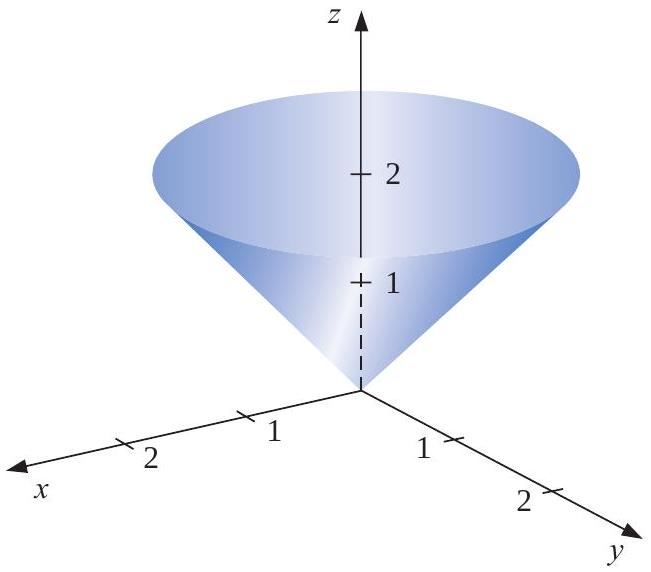
\includegraphics[width=8cm]{2025_05_15_85b7f7df47271a498e1dg-75}
\caption{\scriptsize Figure $6$ }
\label{fig:tripitegillus2}
\end{figure}
%


%Multiple integrals can be evaluated in Maple using the MultInt command in the MultivariateCalculus subpackage of the Student package. For example, to evaluate the multiple integral
%
%$$
%\int_{2}^{4} \int_{x-1}^{x+6} \int_{-2}^{4+y^{2}} x^{2}+y^{2}+z d z d y d x
%$$
%
%we first load the package and define the function with\\[0pt]
%with(Student[MultivariateCalculus]): $f:=(x, y, z) \rightarrow x^{2}+y^{2}+z$\\
%Then issue the command\\
%MultiInt $\left(f(x, y, z), z=-2 . .4+y^{2}, y=x-1 . . x+6, x=2 . .4\right)$\\
%which produces the result\\
%1.995885970

\begin{myexercise}%\label{Comprehensionquiz2}
Consider the following algorithm

\begin{boxB}Algorithm: Simpson's Double Integral\\
To approximate the integral

$$
I=\int_{a}^{b} \int_{c(x)}^{d(x)} f(x, y) d y d x
$$

INPUT endpoints $a, b$ : even positive integers $m, n$.\\
OUTPUT approximation $J$ to $I$.\\
Step 1 Set $h=(b-a) / n$;\\
\hspace*{2cm}$J_{1}=0 ; \quad($ End terms.$)$\\
\hspace*{2cm}$J_{2}=0 ; \quad$ (Even terms.)\\
\hspace*{2cm}$J_{3}=0 . \quad$ (Odd terms.)\\
Step 2 For $i=0,1, \ldots, n$ do Steps 3-8.\\
\hspace*{1cm}Step 3 Set $x=a+i h$; (Composite Simpson's method for $x$.)

$$
\begin{aligned}
& H X=(d(x)-c(x)) / m ; \\
& K_{1}=f(x, c(x))+f(x, d(x)) ; \quad(\text { End terms } .) \\
& K_{2}=0 ; \quad(\text { Even terms } .) \\
& K_{3}=0 . \quad(\text { Odd terms } .)
\end{aligned}
$$

\hspace*{1cm}Step 4 For $j=1,2, \ldots, m-1$ do Step 5 and 6.\\
\hspace*{2.5cm}Step 5 Set $y=c(x)+j H X$;

$$
Q=f(x, y)
$$

\hspace*{2.5cm}Step 6 If $j$ is even then set $K_{2}=K_{2}+Q$\\
\hspace*{4cm} else set $K_{3}=K_{3}+Q$.

Step 7 Set $L=\left(K_{1}+2 K_{2}+4 K_{3}\right) H X / 3$.\\
$\left(L \approx \int_{c\left(x_{i}\right)}^{d\left(x_{i}\right)} f\left(x_{i}, y\right) d y\right.$ by the Composite Simpson's method.)\\
Step 8 If $i=0$ or $i=n$ then set $J_{1}=J_{1}+L$\\
\hspace*{3cm} else if $i$ is even then set $J_{2}=J_{2}+L$ \\
\hspace*{3cm}else set $J_{3}=J_{3}+L$.

%The reduced calculation makes it generally worthwhile to apply\\
%Gaussian quadrature rather than a Simpson's technique when approximating double integrals.

Step 9 Set $J=h\left(J_{1}+2 J_{2}+4 J_{3}\right) / 3$.\\
Step 10 OUTPUT (J); STOP.
\end{boxB}
Use this algorithm with $n=m=4$ to approximate the following double integrals, and compare the results to the exact answers.
\begin{multicols}{2}
\begin{enumerate}[label=(\alph*)]
\item $\int_{2.1}^{2.5} \int_{1.2}^{1.4} x y^{2} d y d x$\\
\item $\int_{0}^{0.5} \int_{0}^{0.5} e^{y-x} d y d x$
\item $\int_{2}^{2.2} \int_{x}^{2 x}\left(x^{2}+y^{3}\right) d y d x$\\
\item $\int_{1}^{1.5} \int_{0}^{x}\left(x^{2}+\sqrt{y}\right) d y d x$
 \end{enumerate}
\end{multicols}
\end{myexercise}

\begin{mysolution}
\begin{multicols}{4}
\begin{enumerate}[label=(\alph*)]
\item $0.3115733$
\item $0.2552526$
\item $16.50864$
\item $1.476684$
 \end{enumerate}
\end{multicols}
\end{mysolution}

\section{Improper Integrals}
\videolesson
\begin{selfvideo}[2]
%LESSON 3: 
This video presents a discussion on numerical methods for improper integrals. Follow the discussion and then solve the problems in the subsequent quiz.
\end{selfvideo}

Improper integrals result when the notion of integration is extended either to an interval of integration on which the function is unbounded or to an interval with one or more infinite endpoints. In either circumstance, the normal rules of integral approximation must be modified.

\subsection*{Left Endpoint Singularity}
We will first consider the situation when the integrand is unbounded at the left endpoint of the interval of integration, as shown in Figure \ref{fig:imprpint1}. In this case we say that $f$ has a singularity at the endpoint $a$. We will then show how other improper integrals can be reduced to problems of this form.

%Figure 4.25\\
\begin{figure}
\centering
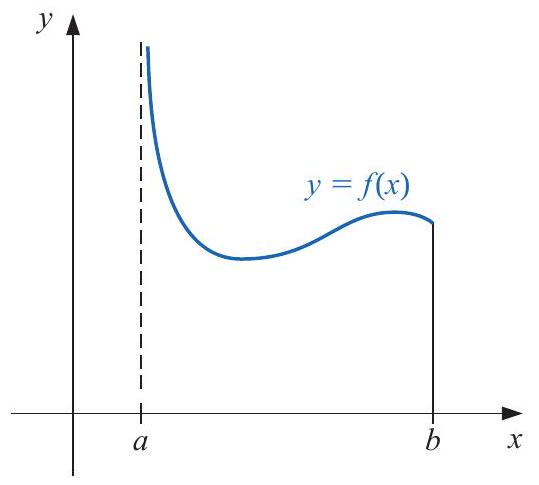
\includegraphics[width=8cm]{2025_05_15_85b7f7df47271a498e1dg-78}
\caption{\scriptsize Figure $7$}
\label{fig:imprpint1}
\end{figure}

It is shown in calculus that the improper integral with a singularity at the left endpoint,

$$
\int_{a}^{b} \frac{d x}{(x-a)^{p}}
$$

converges if and only if $0<p<1$, and in this case, we define

$$
\int_{a}^{b} \frac{1}{(x-a)^{p}} d x=\left.\lim _{M \rightarrow a^{+}} \frac{(x-a)^{1-p}}{1-p}\right|_{x=M} ^{x=b}=\frac{(b-a)^{1-p}}{1-p}
$$

\begin{example}
Show that the improper integral $\int_{0}^{1} \frac{1}{\sqrt{x}} d x$ converges but $\int_{0}^{1} \frac{1}{x^{2}} d x$ diverges.
\end{example}

\begin{mysolution}
For the first integral we have

$$
\int_{0}^{1} \frac{1}{\sqrt{x}} d x=\lim _{M \rightarrow 0^{+}} \int_{M}^{1} x^{-1 / 2} d x=\left.\lim _{M \rightarrow 0^{+}} 2 x^{1 / 2}\right|_{x=M} ^{x=1}=2-0=2
$$

but the second integral

$$
\int_{0}^{1} \frac{1}{x^{2}} d x=\lim _{M \rightarrow 0^{+}} \int_{M}^{1} x^{-2} d x=\lim _{M \rightarrow 0^{+}}-\left.x^{-1}\right|_{x=M} ^{x=1}
$$

is unbounded.

If $f$ is a function that can be written in the form

$$
f(x)=\frac{g(x)}{(x-a)^{p}}
$$

where $0<p<1$ and $g$ is continuous on $[a, b]$, then the improper integral

$$
\int_{a}^{b} f(x) d x
$$

also exists. We will approximate this integral using the Composite Simpson's rule, provided that $g \in C^{5}[a, b]$. In that case, we can construct the fourth Taylor polynomial, $P_{4}(x)$, for $g$ about $a$,

$$
P_{4}(x)=g(a)+g^{\prime}(a)(x-a)+\frac{g^{\prime \prime}(a)}{2!}(x-a)^{2}+\frac{g^{\prime \prime \prime}(a)}{3!}(x-a)^{3}+\frac{g^{(4)}(a)}{4!}(x-a)^{4},
$$

and write


\begin{equation}\label{eqn:impropinteeaxm1eqn1}
\int_{a}^{b} f(x) d x=\int_{a}^{b} \frac{g(x)-P_{4}(x)}{(x-a)^{p}} d x+\int_{a}^{b} \frac{P_{4}(x)}{(x-a)^{p}} d x 
\end{equation}


Because $P(x)$ is a polynomial, we can exactly determine the value of


\begin{equation}\label{eqn:impropinteeaxm1eqn2}
\int_{a}^{b} \frac{P_{4}(x)}{(x-a)^{p}} d x=\sum_{k=0}^{4} \int_{a}^{b} \frac{g^{(k)}(a)}{k!}(x-a)^{k-p} d x=\sum_{k=0}^{4} \frac{g^{(k)}(a)}{k!(k+1-p)}(b-a)^{k+1-p}
\end{equation}


This is generally the dominant portion of the approximation, especially when the Taylor polynomial $P_{4}(x)$ agrees closely with $g(x)$ throughout the interval $[a, b]$.

To approximate the integral of $f$, we must add to this value the approximation of

$$
\int_{a}^{b} \frac{g(x)-P_{4}(x)}{(x-a)^{p}} d x
$$

To determine this, we first define

$$
G(x)= \begin{cases}\frac{g(x)-P_{4}(x)}{(x-a)^{p}}, & \text { if } a<x \leq b, \\ 0, & \text { if } x=a .\end{cases}
$$
\end{mysolution}
This gives us a continuous function on $[a, b]$. In fact, $0<p<1$ and $P_{4}^{(k)}(a)$ agrees with $g^{(k)}(a)$ for each $k=0,1,2,3,4$, so we have $G \in C^{4}[a, b]$. This implies that the Composite Simpson's rule can be applied to approximate the integral of $G$ on $[a, b]$. Adding this approximation to the value in Eq. \ref{eqn:impropinteeaxm1eqn2} gives an approximation to the improper integral of $f$ on $[a, b]$, within the accuracy of the Composite Simpson's rule approximation.

\begin{example}
Use Composite Simpson's rule with $h=0.25$ to approximate the value of the improper integral

$$
\int_{0}^{1} \frac{e^{x}}{\sqrt{x}} d x
$$
\end{example}

\begin{mysolution}
The fourth Taylor polynomial for $e^{x}$ about $x=0$ is

$$
P_{4}(x)=1+x+\frac{x^{2}}{2}+\frac{x^{3}}{6}+\frac{x^{4}}{24},
$$

so the dominant portion of the approximation to $\int_{0}^{1} \frac{e^{x}}{\sqrt{x}} d x$ is

$$
\begin{aligned}
\int_{0}^{1} \frac{P_{4}(x)}{\sqrt{x}} d x & =\int_{0}^{1}\left(x^{-1 / 2}+x^{1 / 2}+\frac{1}{2} x^{3 / 2}+\frac{1}{6} x^{5 / 2}+\frac{1}{24} x^{7 / 2}\right) d x \\
& =\lim _{M \rightarrow 0^{+}}\left[2 x^{1 / 2}+\frac{2}{3} x^{3 / 2}+\frac{1}{5} x^{5 / 2}+\frac{1}{21} x^{7 / 2}+\frac{1}{108} x^{9 / 2}\right]_{M}^{1} \\
& =2+\frac{2}{3}+\frac{1}{5}+\frac{1}{21}+\frac{1}{108} \approx 2.9235450
\end{aligned}
$$

For the second portion of the approximation to $\int_{0}^{1} \frac{e^{x}}{\sqrt{x}} d x$ we need to approximate $\int_{0}^{1} G(x) d x$, where

$$
G(x)= \begin{cases}\frac{1}{\sqrt{x}}\left(e^{x}-P_{4}(x)\right), & \text { if } 0<x \leq 1 \\ 0, & \text { if } x=0\end{cases}
$$



Table \ref{tab:impropinteexam1} lists the values needed for the Composite Simpson's rule for this approximation.\\
Using these data and the Composite Simpson's rule gives

$$
\begin{aligned}
\int_{0}^{1} G(x) d x & \approx \frac{0.25}{3}[0+4(0.0000170)+2(0.0004013)+4(0.0026026)+0.0099485] \\
& =0.0017691
\end{aligned}
$$

Hence

$$
\int_{0}^{1} \frac{e^{x}}{\sqrt{x}} d x \approx 2.9235450+0.0017691=2.9253141
$$

This result is accurate to within the accuracy of the Composite Simpson's rule approximation for the function $G$. Because $\left|G^{(4)}(x)\right|<1$ on $[0,1]$, the error is bounded by

$$
\frac{1-0}{180}(0.25)^{4}=0.0000217
$$\qed
\end{mysolution}
%Table 4.13

\begin{table}[h]
\centering
\begin{tabular}{cl}
\hline
$x$ & \multicolumn{1}{c}{$G(x)$} \\
\hline
0.00 & 0 \\
0.25 & 0.0000170 \\
0.50 & 0.0004013 \\
0.75 & 0.0026026 \\
1.00 & 0.0099485 \\
\hline
\end{tabular}
\caption{}
\label{tab:impropinteexam1}
\end{table}


\subsection*{Right Endpoint Singularity}
To approximate the improper integral with a singularity at the right endpoint, we could develop a similar technique but expand in terms of the right endpoint $b$ instead of the left endpoint $a$. Alternatively, we can make the substitution

$$
z=-x, \quad d z=-d x
$$

to change the improper integral into one of the form


\begin{equation*}
\int_{a}^{b} f(x) d x=\int_{-b}^{-a} f(-z) d z \tag{4.46}
\end{equation*}


which has its singularity at the left endpoint. Then we can apply the left endpoint singularity technique we have already developed. (See Figure \ref{fig:impropintrightep}.)

%Figure 4.26\\
\begin{figure}
\centering
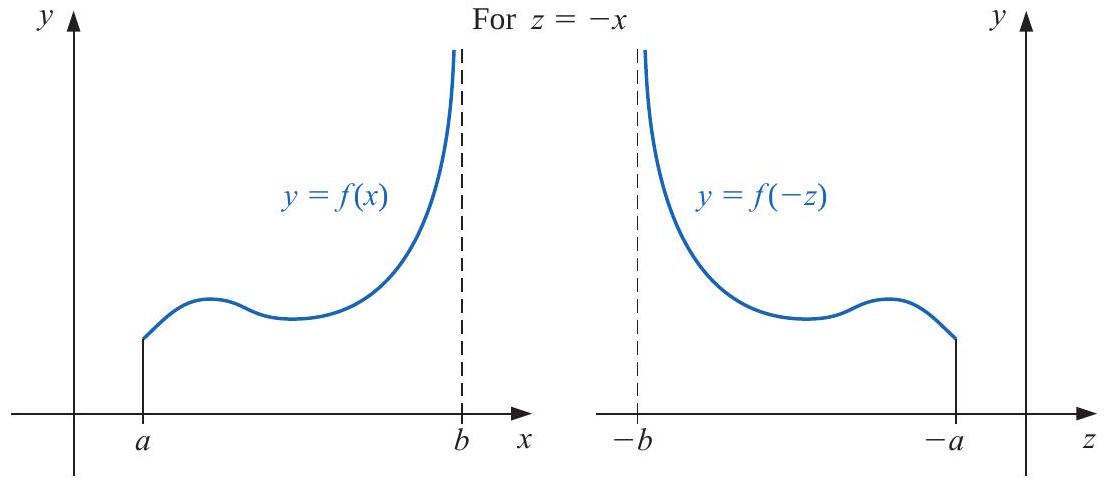
\includegraphics[width=10cm]{2025_05_15_85b7f7df47271a498e1dg-81}
\caption{\scriptsize Figure $8$}
\label{fig:impropintrightep}
\end{figure}

An improper integral with a singularity at $c$, where $a<c<b$, is treated as the sum of improper integrals with endpoint singularities since

$$
\int_{a}^{b} f(x) d x=\int_{a}^{c} f(x) d x+\int_{c}^{b} f(x) d x
$$

\subsection*{Infinite Singularity}
The other type of improper integral involves infinite limits of integration. The basic integral of this type has the form

$$
\int_{a}^{\infty} \frac{1}{x^{p}} d x
$$

for $p>1$. This is converted to an integral with left endpoint singularity at 0 by making the integration substitution

$$
t=x^{-1}, \quad d t=-x^{-2} d x, \quad \text { so } \quad d x=-x^{2} d t=-t^{-2} d t .
$$

Then

$$
\int_{a}^{\infty} \frac{1}{x^{p}} d x=\int_{1 / a}^{0}-\frac{t^{p}}{t^{2}} d t=\int_{0}^{1 / a} \frac{1}{t^{2-p}} d t
$$

In a similar manner, the variable change $t=x^{-1}$ converts the improper integral $\int_{a}^{\infty} f(x) d x$ into one that has a left endpoint singularity at zero:


\begin{equation}\label{eqn:infising}
\int_{a}^{\infty} f(x) d x=\int_{0}^{1 / a} t^{-2} f\left(\frac{1}{t}\right) d t
\end{equation}


It can now be approximated using a quadrature formula of the type described earlier.

\begin{example}
Approximate the value of the improper integral

$$
I=\int_{1}^{\infty} x^{-3 / 2} \sin \frac{1}{x} d x
$$
\end{example}

\begin{mysolution}
We first make the variable change $t=x^{-1}$, which converts the infinite singularity into one with a left endpoint singularity. Then

$$
d t=-x^{-2} d x, \quad \text { so } \quad d x=-x^{2} d t=-\frac{1}{t^{2}} d t
$$

and

$$
I=\int_{x=1}^{x=\infty} x^{-3 / 2} \sin \frac{1}{x} d x=\int_{t=1}^{t=0}\left(\frac{1}{t}\right)^{-3 / 2} \sin t\left(-\frac{1}{t^{2}} d t\right)=\int_{0}^{1} t^{-1 / 2} \sin t d t
$$

The fourth Taylor polynomial, $P_{4}(t)$, for $\sin t$ about 0 is

$$
P_{4}(t)=t-\frac{1}{6} t^{3}
$$

so

$$
G(t)= \begin{cases}\frac{\sin t-t+\frac{1}{6} t^{3}}{t^{1 / 2}}, & \text { if } 0<t \leq 1 \\ 0, & \text { if } t=0\end{cases}
$$

is in $C^{4}[0,1]$, and we have

$$
\begin{aligned}
I & =\int_{0}^{1} t^{-1 / 2}\left(t-\frac{1}{6} t^{3}\right) d t+\int_{0}^{1} \frac{\sin t-t+\frac{1}{6} t^{3}}{t^{1 / 2}} d t \\
& =\left[\frac{2}{3} t^{3 / 2}-\frac{1}{21} t^{7 / 2}\right]_{0}^{1}+\int_{0}^{1} \frac{\sin t-t+\frac{1}{6} t^{3}}{t^{1 / 2}} d t \\
& =0.61904761+\int_{0}^{1} \frac{\sin t-t+\frac{1}{6} t^{3}}{t^{1 / 2}} d t
\end{aligned}
$$

The result from the Composite Simpson's rule with $n=16$ for the remaining integral is 0.0014890097 . This gives a final approximation of

$$
I=0.0014890097+0.61904761=0.62053661
$$

which is accurate to within $4.0 \times 10^{-8}$.
\end{mysolution}
\begin{myexercise}%\label{Comprehensionquiz2}
Use Simpson's Composite rule and the given values of $n$ to approximate the following improper integrals.
\begin{multicols}{2}
\begin{enumerate}[label=(\alph*)]
\item $\int_{0}^{1} x^{-1 / 4} \sin x d x, \quad n=4$\\
\item $\int_{0}^{1} \frac{e^{2 x}}{\sqrt[5]{x^{2}}} d x, \quad n=6$
\item $\quad \int_{1}^{2} \frac{\ln x}{(x-1)^{1 / 5}} d x, \quad n=8$\\
\item $\quad \int_{0}^{1} \frac{\cos 2 x}{x^{1 / 3}} d x, \quad n=6$
\end{enumerate}
\end{multicols}

\begin{mysolution}
The Composite Simpson’s rule gives:
\begin{multicols}{2}
\begin{enumerate}[label=(\alph*)]
\item $0.5284163$
\item $4.266654$
\item $0.4329748$
\item $0.8802210$
\end{enumerate}
\end{multicols}
\end{mysolution}
\end{myexercise}



\section{The Elementary Theory of Initial-Value Problems}
%\activities
%Read on the elementary theory of initial-value problems in pages \textcolor{red}{\bf page $260-264$} of the following reference and then attempt the subsequent quiz
%\begin{activity}[\cg Reading]
%\begin{enumerate}
%\item Burden, R. L., Faires, J. D., Burden, A. M. (2015). Numerical Analysis. Tenth Edition, Cengage Learning.\\
%\end{enumerate}
%\end{activity}
\videolesson
\begin{selfvideo}[2]
%LESSON 3: 
This video presents a discussion on the elementary theory of initial-value problems. Follow the discussion and then solve the problems in the subsequent quiz.
\end{selfvideo}
Differential equations are used to model problems in science and engineering that involve the change of some variable with respect to another. Most of these problems require the solution to a differential equation that satisfies a given initial condition.

In common real-life situations, the differential equation that models the problem is too complicated to solve exactly. One approach in solving such equations uses methods for approximating the solution of the original problem. This approach is most commonly taken because the approximation methods give more accurate results and realistic error information.

The methods that we consider here give approximations found at certain specified, and often equally spaced, points.

We need some definitions and results from the theory of ordinary differential equations before considering methods for approximating the solutions to initial-value problems.

\begin{definition}
A function $f(t, y)$ is said to satisfy a Lipschitz condition in the variable $y$ on a set $D \subset \mathbb{R}^{2}$ if a constant $L>0$ exists with

$$
\left|f\left(t, y_{1}\right)-f\left(t, y_{2},\right)\right| \leq L\left|y_{1}-y_{2}\right|
$$

whenever $\left(t, y_{1}\right)$ and $\left(t, y_{2}\right)$ are in $D$. The constant $L$ is called a {\bf Lipschitz constant} for $f$.
\end{definition}

\begin{example}
Show that $f(t, y)=t|y|$ satisfies a Lipschitz condition on the interval $D=\{(t, y) \mid 1 \leq$ $t \leq 2$ and $-3 \leq y \leq 4\}$.
\end{example}

\begin{mysolution}
For each pair of points $\left(t, y_{1}\right)$ and $\left(t, y_{2}\right)$ in $D$ we have

$$
\left|f\left(t, y_{1}\right)-f\left(t, y_{2}\right)\right|=|t| y_{1}|-t| y_{2}\|=|t|\| y_{1}\left|-\left|y_{2} \| \leq 2\right| y_{1}-y_{2}\right|
$$

Thus $f$ satisfies a Lipschitz condition on $D$ in the variable $y$ with Lipschitz constant 2 . The smallest value possible for the Lipschitz constant for this problem is $L=2$, because, for example,

$$
|f(2,1)-f(2,0)|=|2-0|=2|1-0|
$$
\end{mysolution}

\begin{definition}\label{def:convex}
A set $D \subset \mathbb{R}^{2}$ is said to be convex if whenever $\left(t_{1}, y_{1}\right)$ and $\left(t_{2}, y_{2}\right)$ belong to $D$, then $\left((1-\lambda) t_{1}+\lambda t_{2},(1-\lambda) y_{1}+\lambda y_{2}\right)$ also belongs to $D$ for every $\lambda$ in $[0,1]$.
\end{definition}

In geometric terms, Definition \ref{def:convex} states that a set is convex provided that whenever two points belong to the set, the entire straight-line segment between the points also belongs to the set. (See Figure \ref{fig:convex1}.) The sets we consider in this chapter are generally of the form $D=\{(t, y) \mid a \leq t \leq b$ and $-\infty<y<\infty\}$ for some constants $a$ and $b$. It is easy to verify that these sets are convex.
%
%Figure 5.1\\
\begin{figure}[h]
\centering
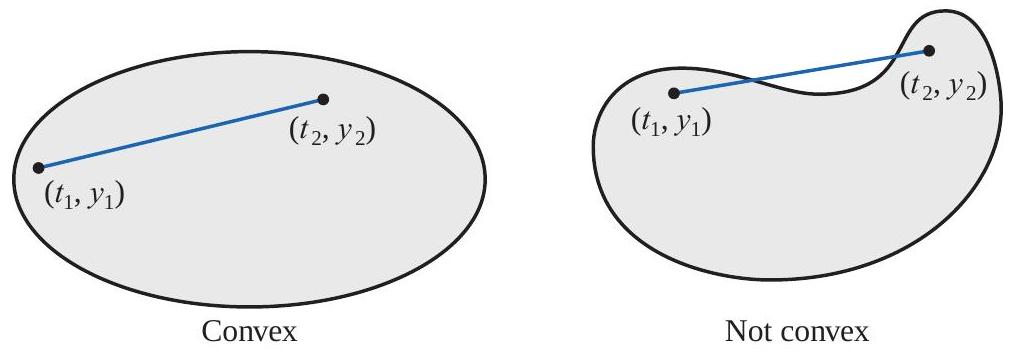
\includegraphics[width=10cm]{2025_05_15_5266fa2c85d567bd073dg-03}
\caption{\scriptsize Figure $10$}
\label{fig:convex1}
\end{figure}

\begin{theorem}\label{thm:elementarytheofIVPtm1}
Suppose $f(t, y)$ is defined on a convex set $D \subset \mathbb{R}^{2}$. If a constant $L>0$ exists with

%Rudolf Lipschitz (1832-1903) worked in many branches of mathematics, including number theory, Fourier series, differential equations, analytical mechanics, and potential theory. He is best known for this generalization of the work of Augustin-Louis Cauchy (1789-1857) and Guiseppe Peano (1856-1932).


\begin{equation}\label{eqn:elementarytheofIVPeq1}
\left|\frac{\partial f}{\partial y}(t, y)\right| \leq L, \quad \text { for all }(t, y) \in D,
\end{equation}


then $f$ satisfies a Lipschitz condition on $D$ in the variable $y$ with Lipschitz constant $L$.
\end{theorem}


As the next theorem will show, it is often of significant interest to determine whether the function involved in an initial-value problem satisfies a Lipschitz condition in its second\\
variable, and condition \ref{eqn:elementarytheofIVPeq1} is generally easier to apply than the definition. We should note, however, that Theorem $1$ gives only sufficient conditions for a Lipschitz condition to hold. The function in Example 1, for instance, satisfies a Lipschitz condition, but the partial derivative with respect to $y$ does not exist when $y=0$.

%The following theorem is a version of the fundamental existence and uniqueness theorem for first-order ordinary differential equations. 

\begin{theorem}\label{thm:elementarytheofIVPtm2}
Suppose that $D=\{(t, y) \mid a \leq t \leq b$ and $-\infty<y<\infty\}$ and that $f(t, y)$ is continuous on $D$. If $f$ satisfies a Lipschitz condition on $D$ in the variable $y$, then the initial-value problem

$$
y^{\prime}(t)=f(t, y), \quad a \leq t \leq b, \quad y(a)=\alpha,
$$

has a unique solution $y(t)$ for $a \leq t \leq b$.
\end{theorem}

\begin{example}
Use Theorem $2$ to show that there is a unique solution to the initial-value problem

$$
y^{\prime}=1+t \sin (t y), \quad 0 \leq t \leq 2, \quad y(0)=0 .
$$
\end{example}

\begin{mysolution}
Holding $t$ constant and applying the Mean Value Theorem to the function

$$
f(t, y)=1+t \sin (t y)
$$

we find that when $y_{1}<y_{2}$, a number $\xi$ in ( $y_{1}, y_{2}$ ) exists with

$$
\frac{f\left(t, y_{2}\right)-f\left(t, y_{1}\right)}{y_{2}-y_{1}}=\frac{\partial}{\partial y} f(t, \xi)=t^{2} \cos (\xi t)
$$

Thus

$$
\left|f\left(t, y_{2}\right)-f\left(t, y_{1}\right)\right|=\left|y_{2}-y_{1}\right|\left|t^{2} \cos (\xi t)\right| \leq 4\left|y_{2}-y_{1}\right|
$$

and $f$ satisfies a Lipschitz condition in the variable $y$ with Lipschitz constant $L=4$. Additionally, $f(t, y)$ is continuous when $0 \leq t \leq 2$ and $-\infty<y<\infty$, so Theorem $2$ implies that a unique solution exists to this initial-value problem.\qed
\end{mysolution}

%If you have completed a course in differential equations you might try to find the exact solution to this problem.
%
\subsection*{Well-Posed Problems}
%Now that we have, to some extent, taken care of the question of when initial-value problems have unique solutions, we can move to the second important consideration when approximating the solution to an initial-value problem. Initial-value problems obtained by observing physical phenomena generally only approximate the true situation, so we need to know whether small changes in the statement of the problem introduce correspondingly small changes in the solution. This is also important because of the introduction of round-off error when numerical methods are used. That is,

\begin{boxB}
\underline{Question:} How do we determine whether a particular problem has the property that small changes, or perturbations, in the statement of the problem introduce correspondingly small changes in the solution?
\end{boxB}

First consider the following workable definition to express this concept.

\begin{definition} 
The initial-value problem

\begin{equation}\label{eqn:wellpossedeq1}
\frac{d y}{d t}=f(t, y), \quad a \leq t \leq b, \quad y(a)=\alpha,
\end{equation}

is said to be a well-posed problem if:

\begin{itemize}
  \item A unique solution, $y(t)$, to the problem exists, and
  \item There exist constants $\varepsilon_{0}>0$ and $k>0$ such that for any $\varepsilon$, with $\varepsilon_{0}>\varepsilon>0$, whenever $\delta(t)$ is continuous with $|\delta(t)|<\varepsilon$ for all $t$ in $[a, b]$, and when $\left|\delta_{0}\right|<\varepsilon$, the initial-value problem


\begin{equation}\label{eqn:wellpossedeq2}
\frac{d z}{d t}=f(t, z)+\delta(t), \quad a \leq t \leq b, \quad z(a)=\alpha+\delta_{0}
\end{equation}

has a unique solution $z(t)$ that satisfies

$$
|z(t)-y(t)|<k \varepsilon \quad \text { for all } t \text { in }[a, b]
$$
\end{itemize}
\end{definition}
The problem specified by \ref{eqn:wellpossedeq2} is called a {\bf perturbed problem} associated with the original problem \ref{eqn:wellpossedeq1}. It assumes the possibility of an error being introduced in the statement of the differential equation, as well as an error $\delta_{0}$ being present in the initial condition.

%Numerical methods will always be concerned with solving a perturbed problem because any round-off error introduced in the representation perturbs the original problem. Unless the original problem is well-posed, there is little reason to expect that the numerical solution to a perturbed problem will accurately approximate the solution to the original problem.

The following theorem specifies conditions that ensure that an initial-value problem is well-posed.

\begin{theorem}\label{thm:wellposedcond}
Suppose $D=\{(t, y) \mid a \leq t \leq b$ and $-\infty<y<\infty\}$. If $f$ is continuous and satisfies a Lipschitz condition in the variable $y$ on the set $D$, then the initial-value problem

$$
\frac{d y}{d t}=f(t, y), \quad a \leq t \leq b, \quad y(a)=\alpha
$$

is well-posed.
\end{theorem}

\begin{example}
Show that the initial-value problem

\begin{equation}\label{eqn:ivpeam3eq}
\frac{d y}{d t}=y-t^{2}+1, \quad 0 \leq t \leq 2, \quad y(0)=0.5
\end{equation}


is well posed on $D=\{(t, y) \mid 0 \leq t \leq 2$ and $-\infty<y<\infty\}$.
\end{example}

\begin{mysolution}
Because

$$
\left|\frac{\partial\left(y-t^{2}+1\right)}{\partial y}\right|=|1|=1
$$

Theorem $1$ implies that $f(t, y)=y-t^{2}+1$ satisfies a Lipschitz condition in $y$ on $D$ with Lipschitz constant $1$. Since $f$ is continuous on $D$, Theorem $3$ implies that the problem is well-posed.

As an illustration, consider the solution to the perturbed problem


\begin{equation}\label{eqn:ivpeam3eq1}
\frac{d z}{d t}=z-t^{2}+1+\delta, \quad 0 \leq t \leq 2, \quad z(0)=0.5+\delta_{0}
\end{equation}

%%Maple reserves the letter $D$ to represent differentiation.\\
where $\delta$ and $\delta_{0}$ are constants. The solutions to Eqs. \ref{} and \ref{} are

$$
y(t)=(t+1)^{2}-0.5 e^{t} \quad \text { and } \quad z(t)=(t+1)^{2}+\left(\delta+\delta_{0}-0.5\right) e^{t}-\delta,
$$

respectively.

Suppose that $\varepsilon$ is a positive number. If $|\delta|<\varepsilon$ and $\left|\delta_{0}\right|<\varepsilon$, then

$$
|y(t)-z(t)|=\left|\left(\delta+\delta_{0}\right) e^{t}-\delta\right| \leq\left|\delta+\delta_{0}\right| e^{2}+|\delta| \leq\left(2 e^{2}+1\right) \varepsilon
$$

for all $t$. This implies that problem \ref{} is well-posed with $k(\varepsilon)=2 e^{2}+1$ for all $\varepsilon>0$.
\end{mysolution}
%Maple can be used to solve many initial-value problems. Consider the problem
%
%$$
%\frac{d y}{d t}=y-t^{2}+1, \quad 0 \leq t \leq 2, \quad y(0)=0.5
%$$
%
%To define the differential equation and initial condition, enter\\
%deq $:=D(y)(t)=y(t)-t^{2}+1$; init $:=y(0)=0.5$\\
%The names deq and init have been chosen by the user. The command to solve the initial-value problems is\\
%deqsol $:=$ dsolve $(\{$ deq, init $\}, y(t))$\\
%and Maple responds with
%
%$$
%y(t)=1+t^{2}+2 t-\frac{1}{2} e^{t}
%$$
%
%To use the solution to obtain a specific value, such as $y(1.5)$, we enter\\
%$q:=\operatorname{rhs}($ deqsol $): \operatorname{evalf}(\operatorname{subs}(t=1.5, q))$\\
%which gives\\
%4.009155465
%
%The function $r h s$ (for $r$ ight $h$ and $s$ ide) is used to assign the solution of the initial-value problem to the function $q$, which we then evaluate at $t=1.5$.
%
%The function dsolve can fail if an explicit solution to the initial-value problem cannot be found. For example, for the initial-value problem given in Example 2, the command\\
%deqsol2 $:=$ dsolve $(\{D(y)(t)=1+t \cdot \sin (t \cdot y(t)), y(0)=0\}, y(t))$\\
%does not succeed because an explicit solution cannot be found. In this case a numerical method must be used.




\begin{myexercise}%\label{Comprehensionquiz2}
Use Theorem \ref{thm:elementarytheofIVPtm2} to show that each of the following initial-value problems has a unique solution, and find the solution.
\begin{enumerate}[label=(\alph*)]
\item $y^{\prime}=y \cos t, \quad 0 \leq t \leq 1, \quad y(0)=1$.\\
\item $y^{\prime}=\frac{2}{t} y+t^{2} e^{t}, \quad 1 \leq t \leq 2, \quad y(1)=0$.\\
\item $y^{\prime}=-\frac{2}{t} y+t^{2} e^{t}, \quad 1 \leq t \leq 2, \quad y(1)=\sqrt{2} e$.\\
\item $y^{\prime}=\frac{4 t^{3} y}{1+t^{4}}, \quad 0 \leq t \leq 1, \quad y(0)=1$.
\end{enumerate}

\begin{mysolution}
\begin{enumerate}[label=(\alph*)]
\item Since $f(t,y) = y\cos t$, we have $\frac{\partial f}{\partial y} (t,y) = \cos t$, and $f$ satisfies a Lipschitz condition in $y$ with $L = 1$ on
\[D=\{(t,y)|0\leq t\leq1,-\infty<y<\infty\}.\]
Also, $f$ is continuous on $D$, so there exists a unique solution, which is $y(t) = e^{\sin t}$.
\item Since $f(t,y) =\frac2t y +t^2e^t$, we have $\frac{\partial f}{\partial y} = \frac2t$, and $f$ satisfies a Lipschitz condition in $y$ with $L = 2$ on
\[D=\{(t,y)|1\leq t\leq2,-\infty<y<\infty\}.\]
 Also, $f$ is continuous on $D$, so there exists a unique solution, which is $y(t) = t^2(e^t-e)$.
\item Since $f(t,y) =-\frac2t y +t^2e^t$,we have $\frac{\partial f}{\partial y}=-\frac2t$, and $f$ satisfies a Lipschitz condition in $y$ with $L = 2$ on
\[D=\{(t,y)|1\leq t\leq2,-\infty<y<\infty\}.\]
Also, $f$ is continuous on $D$, so there exists a unique solution, which is
\[y(t) = (t^4e^t-4t^3e^t + 12t^2e^t-24te^t + 24e^t + (\sqrt{2}-9)e)/t^2.\]
\item Since $f(t,y) = \frac{4t^3y}{1 +t^4}$, we have $\frac{\partial f}{\partial y}=\frac{4t^3}{1 +t^4}$, and $f$ satisfies a Lipschitz condition in $y$ with $L = 2$ on
\[D=\{(t,y)|0\leq t\leq1,-\infty<y<\infty\}.\]
Also, $f$ is continuous on $D$, so there exists a unique solution, which is $y(t) = 1 + t^4$.
\end{enumerate}
\end{mysolution}
\end{myexercise}


\section{Euler's Method}
%\videolesson
%\begin{selfvideo}[2]
%%LESSON 3: 
%This video presents a discussion on Euler's method. Follow the discussion and then solve the problems in the subsequent quiz.
%\end{selfvideo}

\activities
Read on Euler's method in Section 8.02 of the reference whose link is provided below and then attempt the subsequent quiz
\begin{activity}[\cg Reading]
\mylink{https://math.libretexts.org/Workbench/Numerical\_Methods\_with\_Applications\_(Kaw)}
\end{activity}


%\begin{boxB}Question: \end{boxB}
\begin{myexercise}%\label{Comprehensionquiz2}
Use Euler's method to approximate the solutions for each of the following initial-value problems.
\begin{enumerate}[label=(\alph*)]
\item $y^{\prime}=t e^{3 t}-2 y, \quad 0 \leq t \leq 1, \quad y(0)=0$, with $h=0.5$
\item $y^{\prime}=1+(t-y)^{2}, \quad 2 \leq t \leq 3, \quad y(2)=1$, with $h=0.5$
\item $y^{\prime}=1+y / t, \quad 1 \leq t \leq 2, \quad y(1)=2$, with $h=0.25$
\item $y^{\prime}=\cos 2 t+\sin 3 t, \quad 0 \leq t \leq 1, \quad y(0)=1$, with $h=0.25$
\end{enumerate}

\begin{mysolution}
Euler's method gives the approximations in the following table.
\begin{enumerate}[label=(\alph*)]
\item
\begin{center}
\begin{tabular}{cccc}
\hline
$i$ & $t_{i}$ & $w_{i}$ & $y\left(t_{i}\right)$ \\
\hline
1 & 0.500 & 0.0000000 & 0.2836165 \\
2 & 1.000 & 1.1204223 & 3.2190993 \\
\hline
\end{tabular}
\end{center}
\item
\begin{center}
\begin{tabular}{cccc}
\hline
$i$ & $t_{i}$ & $w_{i}$ & $y\left(t_{i}\right)$ \\
\hline
1 & 2.500 & 2.0000000 & 1.8333333 \\
2 & 3.000 & 2.6250000 & 2.5000000 \\
\hline
\end{tabular}
\end{center}
\item
\begin{center}
\begin{tabular}{cccc}
$i$ & $t_{i}$ & $w_{i}$ & $y\left(t_{i}\right)$ \\
\hline
1 & 1.250 & 2.7500000 & 2.7789294 \\
2 & 1.500 & 3.5500000 & 3.6081977 \\
3 & 1.750 & 4.3916667 & 4.4793276 \\
4 & 2.000 & 5.2690476 & 5.3862944 \\
\hline
\end{tabular}
\end{center}
\item
\begin{center}
\begin{tabular}{cccc}
\hline
$i$ & $t_{i}$ & $w_{i}$ & $y\left(t_{i}\right)$ \\
\hline
1 & 0.250 & 1.2500000 & 1.3291498 \\
2 & 0.500 & 1.6398053 & 1.7304898 \\
3 & 0.750 & 2.0242547 & 2.0414720 \\
4 & 1.000 & 2.2364573 & 2.1179795 \\
\hline
\end{tabular}
\end{center}
\end{enumerate}
\end{mysolution}
\end{myexercise}


%\discussion


\begin{posttest}[\textcolor{red}{End of Module 6 Quiz}]
\item Use the algorithm given in Comprehension Quiz of Section $1$ with (i) $n=4, m=8$, (ii) $n=8, m=4$, and (iii) $n=m=6$ to approximate the following double integrals, and compare the results to the exact answers.\\
\begin{multicols}{2}
\begin{enumerate}[label=(\alph*)]
\item $\quad \int_{0}^{\pi / 4} \int_{\sin x}^{\cos x}\left(2 y \sin x+\cos ^{2} x\right) d y d x$
\item $\int_{1}^{e} \int_{1}^{x} \ln x y d y d x$
\end{enumerate}
\end{multicols}
\item Use the transformation $t=x^{-1}$ and then the Composite Simpson's rule and the given values of $n$ to approximate the following improper integrals.
\begin{multicols}{2}
\begin{enumerate}[label=(\alph*)]
\item $\int_{1}^{\infty} \frac{1}{x^{2}+9} d x, \quad n=4$\\
\item $\int_{1}^{\infty} \frac{1}{1+x^{4}} d x, \quad n=4$
\item $\int_{1}^{\infty} \frac{\cos x}{x^{3}} d x, \quad n=6$\\
\item $\quad \int_{1}^{\infty} x^{-4} \sin x d x, \quad n=6$ 
\end{enumerate}
\end{multicols}

\item Consider the following functions: 
\begin{multicols}{2}
\begin{enumerate}[label=(\alph*)]
\item $f(t, y)=t^{2} y+1$
\item $f(t, y)=t y$
\item $f(t, y)=1-y$
\item $f(t, y)=-t y+\frac{4 t}{y}$
\end{enumerate}
\end{multicols}

For each choice of $f(t, y)$ given in parts (a)-(d) above:
\begin{enumerate}[label=\roman*.]
\item Does $f$ satisfy a Lipschitz condition on $D=\{(t, y) \mid 0 \leq t \leq 1,-\infty<y<\infty\}$ ?
\item Can Theorem \label{thm:wellposedcond} be used to show that the initial-value problem


$$
y^{\prime}=f(t, y), \quad 0 \leq t \leq 1, \quad y(0)=1
$$

is well-posed?
\end{enumerate}
\item The actual solutions to the initial-value problems in Comprehension Quiz in Section $4$ are given here. Compare the actual error at each step to the error bound.
\begin{enumerate}[label=\roman*.]
\item $y(t)=\frac{1}{5} t e^{3 t}-\frac{1}{25} e^{3 t}+\frac{1}{25} e^{-2 t}$\\
\item $\quad y(t)=t+\frac{1}{1-t}$\\
\item $\quad y(t)=t \ln t+2 t$\\
\item $y(t)=\frac{1}{2} \sin 2 t-\frac{1}{3} \cos 3 t+\frac{4}{3}$
\end{enumerate}

\begin{mysolution}
 \begin{enumerate}[label=\arabic*.]
\item The given algorithm with $n = 4$ and $m = 8$, $n = 8$ and $m = 4$, and $n = m = 6$ gives:
\begin{enumerate}[label=(\alph*)]
\item $0.5119875, 0.5118533, 0.5118722$
\item $1.718857, 1.718220, 1.718385$
\end{enumerate}

\item The Composite Simpson’s rule gives:
\begin{multicols}{2}
\begin{enumerate}[label=(\alph*)]
\item $0.4112649$ \item $0.2440679$ \item $0.05501681$ \item $0.2903746$
\end{enumerate}
\end{multicols}
\item 
\begin{enumerate}[label=(\alph*)]
\item Lipschitz constant $L=1$; it is a well-posed problem.
\item Lipschitz constant $L=1$; it is a well-posed problem.
\item Lipschitz constant $L=1$; it is a well-posed problem.
\item The function $f$ does not a satisfy Lipschitz condition, so Theorem \label{thm:wellposedcond} cannot be used.
\end{enumerate}
\item 
%\begin{multicols}{2}
\begin{enumerate}[label=(\alph*)]
\item
\begin{center}
\begin{tabular}{ccc}
\hline
$t$ & Actual Error & Error bound \\
\hline
0.5 & 0.2836165 & 11.3938 \\
1.0 & 2.0986771 & 42.3654 \\
\hline
\end{tabular}
\end{center}
\item
\begin{center}
\begin{tabular}{ccc}
\hline
$t$ & Actual Error & Error bound \\
\hline
2.5 & 0.166667 & 0.429570 \\
3.0 & 0.125000 & 1.59726 \\
\hline
\end{tabular}
\end{center}
\item
\begin{center}
\begin{tabular}{ccc}
\hline
$t$ & Actual Error & Error bound \\
\hline
1.25 & 0.0289294 & 0.0355032 \\
1.50 & 0.0581977 & 0.0810902 \\
1.75 & 0.0876610 & 0.139625 \\
2.00 & 0.117247 & 0.214785 \\
\hline
\end{tabular}
\end{center}

\vspace{5mm}
\item
\begin{center}
\begin{tabular}{cc}
\hline
$t$ & Actual Error \\
\hline
0.25 & 0.0791498 \\
0.50 & 0.0906844 \\
0.75 & 0.0172174 \\
1.00 & 0.118478 \\
\hline
\end{tabular}
\end{center}
\end{enumerate}
%\end{multicols}
\end{enumerate}
\end{mysolution}
\end{posttest}

%share your understanding of properties of functions and their applications to solving rates of change problems in physical phenomenon 


%\end{actsoln}

\takehome

\comy{You are now at the last part of this module. Your  task is to do a self-reflection on your learning experience.}



\references
\begin{refenumerate}
\item Kong, Q., Siauw, T., Bayen, A., (2020). Python Programming and Numerical Methods. First Edition, Academic Press,  ISBN-13 ‏ : ‎ 978-0128195499 \\
%chapter 1 pg 7-36 functions\\
%chapter 1 pg 51-83 limits and continuity\\
%chapter 1 pg 45-50 rates of change\\
%chapter 2 pg 108-120 the derivative\\
%\item Mendelson, E. (2022). Schaum's Outline of Calculus. McGraw-Hill Education.
%chapter 6 51-55 functions
%chapter 7 59-65 limits
%chapter 8 69-74 continuity
%chapter 9 77-81 derivative
%\item Calculus \mylink{https://math.libretexts.org/Bookshelves/Calculus}
%\item Chris McMullen, 2021, Essential Calculus Skills Practice Workbook with Full Solutions, Zishka Publishing, ISBN 978-1-941691-24-3
%\item R. Adams and C. Essex, 2021, Calculus: A complete Course, Addison Wesley, ISBN 13: 978-0135732588
%\item P. Abbott and H. Neill, 2018, Calculus: A Complete Introduction: The Easy Way to Learn Calculus (Teach Yourself), ISBN 13: 978-1473678446
\end{refenumerate}





%\wrapup
%To wrap-up, answer the following questions:
%
%\begin{enumerate}
%\item 
%%when do we say that a limit of a function exists?
%%\item how do we remove discontinuity in functions?
%%\item what is the relationship between the gradient of the tangent line and the derivative?
%\end{enumerate}
















%\newpage

%\facilitation


%
\begin{center}
    {\Large \textbf{FUNCTIONS OF SEVERAL VARIABLES}}\\[2mm]
(DEFINITION, DOMAIN, RANGE, GRAPHS AND LEVEL CURVES) \\[4mm]

\mycenterbox{5 minute review}%\\[4mm]
Recap the definition of a function of several variables, and the meaning of domain, range, graph and level curves of functions of several variables.
\end{center}
\mycenterbox{Warm-up.}%\\[4mm]
\problemAnswer{
Match the function with its graph (labeled I–VI).Give reasons for your choices
\begin{multicols}{3}
\begin{enumerate}[label=(\alph*)]
\item $f(x,y)=|x|+|y|$\\[4mm]
\item $f(x,y)=|xy|$
\item $f(x,y)=\frac{1}{1+x^2+y^2}$\\2mm]
\item $f(x,y)=(x^2-y^2)^2$
\item $f(x,y)=(x-y)^2$\\[4mm]
\item $f(x,y)=\sin(|x|+|y|)$
\end{enumerate}
\end{multicols}

\begin{center}
%\centering
\includegraphics[width=10cm]{MCTutorial1Q1.JPEG}
\end{center}
%\tcbox[tcbox raise base]{Warm-up}
 
%\begin{flushright}
%\begin{tikzpicture}
%    % A body
%
%
%    % Non-rectangle shapes must be drawn as polygone
%    \begin{scope}[shift={(3,0)}]
%        \draw  (0,0.5) -- (0,4) -- (.5,4) -- (.5,4.5) -- (1.,4.5) -- (4.,4.5) --(4.,4)-- (4.5,4) --(4.5,0.5) --(4.0,0.5)--(4.0,0.0)-- (.5,0) --(0.5,0.5) -- cycle;
%        % Draw symmetry lines
%        \draw [symmetry] (.5, 0.5) -- (.5,4.0);
%        \draw [symmetry] (4, 0.5) -- (4,4.0);
%        \draw [symmetry] (.5,4.0) -- (4,4.0);
%         \draw [symmetry] (.5, 0.5) -- (4, 0.5);
%        % Dimensions
%        \draw (4.5,0) -- ++(0.5,0) coordinate (D1) -- +(5pt,0);
%        \draw (4.5,4.5) -- ++(0.5,0) coordinate (D2) -- +(5pt,0);
%        \draw [dimen] (D1) -- (D2) node {6cm};
%       
%        
%        \draw (0.0,5) -- ++(0,0.5) coordinate (D1) -- +(0,+5pt);
%        \draw (0.5,5) -- ++(0,0.5) coordinate (D2) -- +(0,+5pt);
%        \draw [dimen,-] (D1) -- (D2) node [above=5pt] {$x$ cm};
%        \draw [dimen,<-] (D1) -- ++(-5pt,0);
%        \draw [dimen,<-] (D2) -- ++(+5pt,0);
%    \end{scope}
%\end{tikzpicture}
%\end{flushright}

}


\mycenterbox{Problems.}%

%\begin{center}
%\tcbox[tcbox raise base]{ Problems. Choose from the below}
%\end{center}
\problem{Exploring functions}%
\begin{enumerate}[(a)]
\item Are the following functions even, odd, or neither? What can you say
about their range?
\begin{multicols}{4}
 \begin{enumerate}[(i)]
\item $\displaystyle \frac{3x}{x^2+2}$
\item $\displaystyle \cos x+3$
\item $\displaystyle \frac{2x^3}{\cos x+3}$
\item $\displaystyle \frac{3x^4+2x^2}{\sin x+4}$
\end{enumerate}
\end{multicols}
\item Consider the functions $\sin^n x$ and $\cos^n x$, where $n$ is a positive integer.
Which are odd, which are even, and what are their periodicities?
\item What is the periodicity of $f(x) = 2 \cos x+\sin 2x$? Is it even/odd/neither?

\end{enumerate}

\problem{Cubic functions} 
Show that $x-1$ is a factor of the cubic function%
$$P(x)=x^3-2x^2-5x+6,$$
and  find the quadratic factor $Q(x)$ such that $P(x) = (x -1)Q(x)$. Factorise
$Q(x)$ and hence sketch $P(x).$

%\newpage
\problem{Sigmoid functions*.}%
For positive integers $n$, consider the family of functions
$$\displaystyle f_n= \frac{x^n}{2^n+x^n}.$$
\begin{enumerate}[(a)]
\item What are appropriate domains and ranges for $f_n(x)$? Do they depend on $n$?

\item Is $f_n(x)$ even, odd, or neither? Does this depend on $n$?

\item Show that for $x\geq 0$, $f_n(x)$ are strictly increasing functions and that
$0\leq f_n(x) < 1.$
\item What is the value of $f_n(2)$? Does it depend on $n$?

\item By considering the values of $f_n(1.9)$ and $f_n(2.1)$ for $n = 2, 4, 8, 16, 32$ and
$64$, show that the graph of $f_n(x)$ for $x\ge 0$ is an increasing sigmoid (that
is, $S$-shaped) function that approaches a step function as $n\rightarrow \infty$.
\end{enumerate}

\mycenterbox{Selected answers and hints}%

For the warm-up, $V(x)=4x(3-x)^2$. Writing $x=1+\epsilon$, we get
$$V = 4(1 +\epsilon)(3- (1+\epsilon))^2=4(4-\epsilon^2(3-\epsilon)).$$
If $-1<\epsilon<2$ then $\epsilon^2 (3-\epsilon)\ge 0$, with equality when $\epsilon=0$. Thus the maximum
value of $V$ occurs when $\epsilon= 0$, i.e. $x = 1\rm{cm}$.

\begin{enumerate}
\item 
\begin{enumerate}[(i)]
\item Odd. The range is the interval  $[-\frac{3}{4}\sqrt{2},\; \frac{3}{4}\sqrt{2}]$
\item Even. The range is the interval $[2, 4]$.
\item Odd. The range is all of $\mathbb R$.
\item Neither. (For example, writing $\displaystyle \frac{5}{\sin x+4}$ we have $\displaystyle f(1)= \frac{5}{\sin (1)+4} \equiv 1.032 (3\rm{dp})$ which is neither $f(1)$ nor $-f(1)$.)\\[4mm]
The range is the nonnegative reals $[0,\infty)$

\end{enumerate}
\end{enumerate}











%
%\newpage
%
%\newpage
%
%
%\newtheorem{definition}[subsection]{Definition}
%\newtheorem{example}[subsection]{Example}
\newtheorem{cor}[subsection]{Corollary}
\newtheorem{pro}[subsection]{Proposition}
\newtheorem{theo}[subsection]{Theorem}
\newtheorem{lem}[subsection]{Lemma}
%\newtheorem{rem}[subsection]{Remark}

\definecolor{main}{HTML}{5989cf}    % setting main color to be used
\definecolor{sub}{HTML}{cde4ff}     % setting sub color to be used

\tcbset{
    sharp corners,
    colback = white,
    before skip = 0.2cm,    % add extra space before the box
    after skip = 0.5cm      % add extra space after the box
}                           % setting global options for tcolorbox

% You can copy any following box you like to your code.
\newtcolorbox{boxA}{
    fontupper = \bf,
    boxrule = 1.5pt,
    colframe = black % frame color
}

\newtcolorbox{boxB}{
    fontupper = \bf\color{main}, % font color
    boxrule = 1.5pt,
    colframe = main,
    rounded corners,
    arc = 5pt   % corners roundness
}
\newtcolorbox{boxC}{
    colback = sub, % background color
    boxrule = 0pt  % no borders
}

\newtcolorbox{boxD}{
    colback = sub, 
    colframe = main, 
    boxrule = 0pt, 
    toprule = 3pt, % top rule weight
    bottomrule = 3pt % bottom rule weight
}

\hypersetup{
    colorlinks=true,
    linkcolor=blue,
    filecolor=magenta,      
    urlcolor=cyan,
    pdftitle={Overleaf Example},
    pdfpagemode=FullScreen,
    }

\urlstyle{same}


\coursetitle{\mtthreeiii}{MT303}
\developers{Wyclife Rao}
\reviewers{Dr Irene Sitawa}
\modulenumber{7}
\modulename{Initial-Value Problems for Ordinary Differential Equations}

% courses
\thispagestyle{empty}
\begin{tikzpicture}[overlay,remember picture,font=\sffamily\bfseries]
 \draw[ultra thick,c4,name path=big arc] ([xshift=-2mm]current page.north) arc(150:285:11) coordinate[pos=0.225] (x0);
 \begin{scope}
  \clip ([xshift=-2mm]current page.north) arc(150:285:11) --(current page.north east);
  \fill[c4!50,opacity=0.25] ([xshift=4.55cm]x0) circle (4.55);
  \fill[c4!50,opacity=0.25] ([xshift=3.4cm]x0) circle (3.4);
  \fill[c4!50,opacity=0.25] ([xshift=2.25cm]x0) circle (2.25);
  \draw[ultra thick,c4!50] (x0) arc(-90:30:6.5);
  \draw[ultra thick,c4] (x0) arc(90:-30:8.75);
  \draw[ultra thick,c4!50,name path=arc1] (x0) arc(90:-90:4.675);
  \draw[ultra thick,c4!50] (x0) arc(90:-90:2.875);
  \path[name intersections={of=big arc and arc1,by=x1}];
  \draw[ultra thick,c4,name path=arc2] (x1) arc(135:-20:4.75);
  \draw[ultra thick,c4!50] (x1) arc(135:-20:8.75);
  \path[name intersections={of=big arc and arc2,by={aux,x2}}];
  \draw[ultra thick,c4!50] (x2) arc(180:50:2.25);
 \end{scope} 
 \path[decoration={text along path,text color=c4,
                 raise = -2.8ex,
                 text  along path,
                 text = {},%|\sffamily\bfseries|02/18/2019
                 text align = center,
             },
             decorate
         ] ([xshift=-2mm]current page.north) arc(150:245:11);
 %
 \newcommand\add{4cm}
 \begin{scope}%[shift={(5,0)}]
  \path[clip,postaction={fill=c3}]
  ([xshift=2cm+\add,yshift=-8cm]current page.center) rectangle ++ (4.6,7.7);
  \draw[c5,ultra thick,fill=c2] ([xshift=0.5cm+\add,yshift=-8cm]current page.center)
   ([xshift=0.5cm+\add,yshift=-8cm]current page.center)  arc(180:60:2)
    |- ++ (-3,6) --cycle;
  \draw[ultra thick,c5] ([xshift=-1.5cm+\add,yshift=-8cm]current page.center) 
  arc(180:0:2);
  \draw[ultra thick,c5] ([xshift=0.5cm+\add,yshift=-8cm]current page.center) 
  arc(180:0:2);
  \draw[ultra thick,c5] ([xshift=2.5cm+\add,yshift=-8cm]current page.center) 
  arc(180:0:2);
  \draw[ultra thick,c5] ([xshift=4.5cm+\add,yshift=-8cm]current page.center) 
  arc(180:0:2);
  \fill[white] ([xshift=2.5cm+\add,yshift=-8cm]current page.center) +(60:2) circle(1.5mm)
  node[above
  right=0mm,text=c5!80!black]{$\rho:=\dfrac{1+\sqrt{-3}}{2}$};
 \end{scope}
 %
 \fill[c1] ([xshift=2cm+\add,yshift=-8cm]current page.center) rectangle ++ (-30.7,7.7);
 \node[text=white,anchor=west,scale=2.3,inner sep=0pt] at
 ([xshift=-10cm,yshift=-1.8cm]current page.center) {\color{ulabgold} LEARNING};
 \node[text=white,anchor=west,scale=5,inner sep=0pt] at
 ([xshift=-10cm,yshift=-3.25cm]current page.center) {MODULE \dpmdnumber};
 \node[text=white,anchor=west,scale=2.5,inner sep=0pt,text width=.4\textwidth] at
 ([xshift=-10cm,yshift=-6cm]current page.center) {\dpmdname};
 \node[text=white,anchor=east,scale=2,inner sep=0pt] at
 ([xshift=5.7cm,yshift=-7.5cm]current page.center) {\color{ulabgold}The Open University of Kenya};
 %
% \draw[gray,line width=5mm] 
% ([xshift=2mm,yshift=-1mm]current page.south west) rectangle ([xshift=-2mm,yshift=1mm]current
% page.north east);
\end{tikzpicture}

%\newpage
\pagenumbering{roman}
\thispagestyle{empty}%firstpage


\begin{center}
\vspace*{2cm}
{\Huge\bf BACHELOR OF TECHNOLOGY EDUCATION}\\[3cm]  


%{\fontsize{80}{40}\selectfont \dpcoursecode}\\[2cm]
%
%{\fontsize{30}{40} \selectfont \dpcoursename}\\[2cm]

%\rule{\textwidth}{1pt}
%\vspace{2cm}

%{\fontsize{40}{40}\selectfont \bf Module~\dpmdnumber}\\[2cm]
%
%{\fontsize{30}{40}\selectfont \bf \dpmdname}\\

\vfill
\begin{flushright}
\begin{minipage}{.6\textwidth}
\begin{tcolorbox}%[text ]
\begin{tabular}{ll}%\hline
\subtitle{Developed by:}&\displaydevelopers\\
&\\
\subtitle{Reviewed by:}&\makecell[l]{\displayreviewers}\\
\end{tabular}
\end{tcolorbox}
\end{minipage}\hspace*{-3.5cm}
\end{flushright}
\vspace*{-2.5cm}
\end{center}

\newpage
\thispagestyle{empty}
\null
\vfill
{\renewcommand\arraystretch{1.5}
\begin{tabular}{|l|l|}\hline
\subtitle{Programme Title} & Bachelor of Technology Education \\\hline
\subtitle{Course Title} & \fullcoursename\\\hline
\subtitle{Learning Module number} & Module \dpmdnumber\\\hline
\subtitle{Learning module title} & \dpmdname \\\hline
\subtitle{Module Developer} & \displaydevelopers\\\hline
\subtitle{Reviewed by} & \displayreviewers\\\hline
%\subtitle{Vision} & \vision\\\hline
%\subtitle{Audience description} & \\\hline
\end{tabular}}
\clearpage

%\section{COURSE LEARNING GUIDE}


\subsection*{Preparing for Online and Distance Learning}

This course offers you the opportunity to enter an online space where you can engage with fellow students at the university. The online forums, exercises, tasks and materials have been designed by the course facilitators in such a way that you can draw directly from their knowledge and share in their scholarly interest in online learning and assessment

We hope you will use your access to this virtual classroom to raise all your questions on the course module, to build a network great learners and to share your own thoughts and experiences to the benefit of your fellow students.

   
There are a number of steps you can take to ensure you are well prepared to make the most of this learning opportunity. This resource should prompt you to consider the following:


 \begin{enumerate}[label=\cb$\square$]
   \item How can you best prepare the space where you expect you will spend most of your time engaging in online learning (i.e. in your home or office, or even during your commute to work or whilst traveling)?
  \item   What can you do to ensure you keep working through the course material, even when you do not have Internet access?
    \item How can you familiarise yourself with the course layout, in order to be able to navigate through the steps with ease?
    \item What are the communication strategies and best practices you could consider to best engage with your fellow students and the course facilitators?
    \item What do you do when you need academic or technical support?

 \end{enumerate} 

\subsection*{General Module Guide}

The authors of this module believe that imparting knowledge should always be a mutual relationship between the students and the teachers. Students can actively construct knowledge through experiences gained in reading and answering the learning modules.

You should take time to read everything written in the module, actively and religiously solve all the exercises included to finish this course and be able to gain all the competencies and skills expected to demonstrate the learning outcomes as stated in this course. If you finish with full confidence that you understand and can apply all the knowledge you gain in this course, then you are sure to succeed in tackling the next higher subjects in your chosen course.

In this course, you will be taught not only the knowledge you need to demonstrate your learning outcomes, but you will also gain discipline, perseverance, higher thinking skills, and resourcefulness that would help strengthen your foundation to succeed in life. To successfully finish the course, you must follow the guides set forth in using this module.


\begin{description}[{format=\textcolor{ulabblue}}]
\item[STUDY ENVIRONMENT.]\leavevmode\\
Before engaging into the module, make sure that you are comfortable enough and diminish distractions. Make sure that you develop a study routine to perform and accomplish all the activities set forth by the module.
%\newpage

\item[MODE OF DELIVERY.]\leavevmode\\
Students are required to get a access a digitised copy of the module from the Virtue Learning Environment. As an open and distance learner, you should be able to learn independently and optimise the learning modes and environment available to you as much of  the delivery of all the lessons will be done asynchronously. Your success will greatly depend on your self-motivation and discipline to get your work done without your instructor to remind you from time to time.

\item[STUDY SCHEDULE.] \leavevmode\\
Remember that you have other subjects to attend to, hence, you must manage your time so that you will not be left behind in any of them. Create your own learning plan for each course to make sure that you can perform all the activities. Do not procrastinate your work, remember that time wasted can never be retrieved back. Make sure that even if you are at home, you are a student enrolled in a program, where the learning of all its courses greatly depends on your will to learn as the materials you need are all in your hands. So always be aware of your daily tasks.

\item[PRACTICE EXERCISE.]\leavevmode\\
To measure your learning from your reading, you are given practice exercises which you are supposed to answer daily. This will prepare you in performing your main task.

\item[ONLINE GROUP CHAT.]\leavevmode\\
I am going to create an online Discussion Forum and QA Forum  on the VLE.  This will serve as a room for discussion on the topics and activities found in your module.

\item[RECOMMENDED REFERENCES FOR SUPPLEMENTARY READING.]\leavevmode\\
You are given links that you need to access online. These links are online references such as e-books, online activities, and tutorial videos of the topic. These are other references you can use to further understand the topic and gain additional knowledge and skills.

\item[MAIN TASK.]\leavevmode\\
You are given a task that will require you to apply the knowledge and skills you learned from the module. This can be a group or individual activity which will measure your higher order thinking skills you acquired throughout the topic.

\item[RUBRICS. ]\leavevmode\\
This is a tool to guide you in performing your main task. Through this, you will be able to know the specific indicators that should be found in your task. This is to assess your constructive behaviour towards your learning application. You will be rated according to a 4-point scale shown below.
\begin{center}
{\color{ulabgold} \bf 4 − Excellent\quad\quad   3 −Good\quad\quad    2 − Fair \quad\quad  1 −Poor}
\end{center}
\item[REFLECTIONS.]\leavevmode\\
Writing your reflection will be a passageway to express your experiential learning in using this module. In your honest recall, write everything that you think happened to you during your learning experience in this module. Use the guide questions below:
\begin{description}[{format=\textcolor{ulabblue}}]
\item[First paragraph. ]\leavevmode\\
How was your learning experience? Maybe you can consider describing the effect of the parts of the module (sequence, discussions, examples, practice exercises, online activities, and the main task) in your learning experience. You can point out the strength and weakness of each part so that we can consider it for future improvement of this instructional material.
\item[Second paragraph.  ]\leavevmode\\
What did you learn? Did you successfully acquire the learning outcomes?

\item[Third paragraph.]\leavevmode\\
How can you use what you learned in the future?
\end{description}
\end{description}

\section{ASSESSMENT  TASKS \& EXAMINATION   RULES AND GUIDELINES}

\begin{enumerate}[label=\cb\arabic*.]
\item {\cb SUBMISSION OF ASSESSMENT TASTS.}

Since mathematical skills are best acquired through constant practice, you are encouraged to answer at least two (2) exercises a day. These practice exercises will not be graded but it will help you develop your thinking skills which will prepare you in the performance of your main tasks. You are required to submit your practice exercises every week.
\begin{center} {\cg Usually submission deadlines are set on Saturday 11:59PM EAT} \end{center}

\item  {\cb GROUP CHAT.}

You can post questions, solutions, and comment to other's post. Please be reminded that our group chat is exclusive only for discussion on topics related to this course. Everyone is required to actively participate in the discussions. Also, trolling is highly discouraged. Always observe proper online etiquettes when participating in discussions.
\begin{center} {\cb RULE OF THUMB: ALWAYS THINK BEFORE YOU CLICK} \end{center}

\item  {\cb MAIN TASK. }

Complete documentation during the preparation of your task is required to ensure that every member of the group participated and contributed in the task. May it be photos or screenshots of your virtual meetings or group works. You are going to submit it as attachment of your main task the same way as the practice exercises.



\item {\cb RECOMMENDED REFERENCES FOR SUPPLEMENTARY READING.} 

You can explore online for other references that is related to the topic to gain additional information about the topic. Do not share or post inappropriate materials online or even privately.
\end{enumerate}

\subsection*{Requirements to pass the course}

Compiled Continuous  Assignment/Activities and Tasks  with Final Performance Examination.

\subtitle{Grading System}
\begin{center}
{\renewcommand\arraystretch{1.5}
\begin{tabular}{|l|c|}\hline
Continuous Activities and Tasks  &  50\%\\\hline
Final Performance Examination. &  50\%\\\hline
\end{tabular}
}
\end{center}
%\newpage










%\subsection{INTRODUCTORY MESSAGE}

%A warm welcome to \;  \fullcoursename, {\bf Module on \dpmdname}.



%By this module learning resource, we aim to enable you  achieve the relevant competencies, depict skill, action and purpose successfully. 
 

%It has been designed to provide you with fun and meaningful opportunities for guided and independent learning at your own pace and time. You will be enabled to process the contents of the learning material while being an active learner. Your academic success lies in your own hands.  This module has the following parts and corresponding icons:





{
\renewcommand\arraystretch{4}
\begin{longtblr}{
width=\linewidth,
 colspec={ Q[1,c,f] Q[1.5,r,m] Q[4,l,m] },
%row{1} = { font=\bfseries },
% rowhead = 1,
  caption={ }, 
  label={ },
  rowsep = 4pt,
  hlines = {ulabblue!20, 1pt},
  vlines = {ulabblue!20, 1pt},
}

\includegraphics[width=2cm]{img/audience} & {\bf AUDIENCE}  &  This is a description of a target audience.   \\
{\fontsize{40}{30}\selectfont\color{ulabblue}\faCogs}& {\bf MODULE DESCRIPTION} & 
This part explains the importance of the topics discussed in the module. It will also give you a sneak peek of what you will learn and what is expected from you at the end of the module.\\

\includegraphics[width=2cm]{img/target.png} &  {\bf  EXPECTATION} & These are what you will be able to know after completing the lessons in the module\\

\includegraphics[width=2cm]{img/preactivities} & {\bf PRE-ACTIVITY} &
This activity is to get you set, activate and engage schema to learn the module. Through this activity, you will know the relevance of this activity to the topic that will be discussed in the module.\\

\includegraphics[width=2cm]{img/pretest} &  {\bf PRE - ASSESSMENT} & This will measure your prior knowledge and the concepts to be mastered throughout the lesson. \\

\includegraphics[width=1.7cm]{img/rewind} &  {\bf  RECAP} & This section will measure what learnings and skills that you understand from the previous lesson.\\

\includegraphics[width=1.5cm]{img/lesson} &  {\bf  LESSON} & This section will discuss the topic for this module.\\

\includegraphics[width=2cm]{img/activities} &  {\bf  ACTIVITIES} & This is a set of activities you will perform.\\

\includegraphics[width=2cm]{img/summary} &  {\bf  WRAP UP} & This section summarizes the concepts and applications of the lessons.\\

\includegraphics[width=2cm]{img/discussion}& {\bf DISCUSSIONS} &
This is the meat of the module. The discussion is aligned to the topic learning outcomes that is expected of you to acquire at the end of the module.\\

\includegraphics[width=1.8cm]{img/value} &  {\bf  VALUING} & This part will check the integration of values in the learning competency you will take home.\\

\includegraphics[width=1.8cm]{img/posttest} &  {\bf  POST - ASSESSMENT} & This will measure how much you have learned from the entire module.\\

\includegraphics[width=1.8cm]{img/selfreflect} & {\bf REFLECTION }
&
This part is for you to share your thoughts by writing your reflection, make sure to check your grammar and spelling to ensure the readability and so that it will not alter the thought being delivered. 
\end{longtblr}
}









%\vfill

\audience
\begin{oldactivity}{Audience Description}{
\includegraphics[width=22mm]{img/audience}}{}
This module is offered to all students taking the Bachelor of Technology Education. As an open and distance learner, you should be able to learn independently and optimise the learning modes and environment available to you. Before you begin this course, please confirm the course material, the course requirements and how the course is conducted.
\end{oldactivity}
%\newpage
\pagenumbering{arabic}



\mddescription
This module guides you into a detailed discussion of the concepts of nemrical methods for initial-value problems for ordinary differential equations. Specificcally you will learn about
\begin{itemize}
\item higher-order Taylor methods
\item Runge-Kutta methods
\item error control and Runge-Kutta-Fehlberg method
\item multistep methods 
\end{itemize}
%\expectations
%\begin{objenumerate}
%
%\end{objenumerate}

\begin{mlos}
\item Define the Runge-Kutta family of methods and multistep approaches.
\item Explain error control strategies in Runge-Kutta methods.
\item Implement Runge-Kutta and multistep methods to solve ODE initial value problems.
\item Assess the impact of variable step-size on the accuracy and efficiency of numerical solvers. 
\end{mlos}

\section{Higer-Order Taylor Methods}
\activities
Read on on higher-order Taylor methods in the reference provided in the link below in Section 3.3 and then attempt the subsequent quiz.
\begin{activity}[\cg Reading]
\end{activity}
\mylink{https://math.libretexts.org/Bookshelves/Differential\_Equations/\\A\_First\_Course\_in\_Differential\_Equations\_for\_Scientists\_and\_Engineers\_(Herman)}

%\videolesson
%\begin{selfvideo}[1]
%%LESSON 3: 
%This video presents a discussion on higher-order Taylo methods. Follow the discussion and then solve the problems in the subsequent quiz.
%\end{selfvideo}
%\begin{boxB}Question: \end{boxB}
\begin{myexercise}%\label{Comprehensionquiz2}
Use Taylor's method of order two to approximate the solutions for each of the following initial-value problems.\\
\begin{enumerate}[label=(\alph*)]
\item $ y^{\prime}=t e^{3 t}-2 y, \quad 0 \leq t \leq 1, \quad y(0)=0$, with $h=0.5$\\
\item $y^{\prime}=1+(t-y)^{2}, \quad 2 \leq t \leq 3, \quad y(2)=1$, with $h=0.5$
%\item  $y^{\prime}=1+y / t, \quad 1 \leq t \leq 2, \quad y(1)=2$, with $h=0.25$\\
%\item $y^{\prime}=\cos 2 t+\sin 3 t, \quad 0 \leq t \leq 1, \quad y(0)=1$, with $h=0.25$
\end{enumerate}


\begin{mysolution}
\begin{enumerate}[label=(\alph*)]
\item
\begin{center}
\begin{tabular}{ccc}
\hline
$t_{i}$ & $w_{i}$ & $y\left(t_{i}\right)$ \\
\hline
0.50 & 0.12500000 & 0.28361652 \\
1.00 & 2.02323897 & 3.21909932 \\
\hline
\end{tabular}
\end{center}

\vspace{2mm}

\item
\begin{center}
\begin{tabular}{ccc}
\hline\hline
$t_{i}$ & $w_{i}$ & $y\left(t_{i}\right)$ \\
\hline
1.25 & 2.78125000 & 2.77892944 \\
1.50 & 3.61250000 & 3.60819766 \\
1.75 & 4.48541667 & 4.47932763 \\
2.00 & 5.39404762 & 5.38629436 \\
\hline
\end{tabular}
\end{center}

%\vspace{2mm}
%
%\item
%\begin{center}
%\begin{tabular}{ccc}
%\hline
%$t_{i}$ & $w_{i}$ & $y\left(t_{i}\right)$ \\
%\hline
%2.50 & 1.75000000 & 1.83333333 \\
%3.00 & 2.42578125 & 2.50000000 \\
%\hline
%\end{tabular}
%\end{center}
%
%\vspace{2mm}
%
%\item
%\begin{center}
%\begin{tabular}{ccc}
%\hline\hline
%$t_{i}$ & $w_{i}$ & $y\left(t_{i}\right)$ \\
%\hline
%0.25 & 1.34375000 & 1.32914981 \\
%0.50 & 1.77218707 & 1.73048976 \\
%0.75 & 2.11067606 & 2.04147203 \\
%1.00 & 2.20164395 & 2.11797955 \\
%\end{tabular}
%\end{center}
\end{enumerate}
\end{mysolution}
\end{myexercise}

\section{Runge-Kutta Methods}
%\begin{youtube}
%This video presents a discussion on Runge-Kutta methods. Follow the discussion and then solve the problems in the subsequent quiz.
%\end{youtube}
\activities
Read on on Runge-Kutta methods in the reference provided in the link below in Section 3.4 and then attempt the subsequent quiz.
\begin{activity}[\cg Reading]
\end{activity}
\mylink{https://math.libretexts.org/Bookshelves/Differential\_Equations/\\A\_First\_Course\_in\_Differential\_Equations\_for\_Scientists\_and\_Engineers\_(Herman)}

\begin{myexercise}%\label{Comprehensionquiz2}
Use the Modified Euler method to approximate the solutions to each of the following initial-value problems, and compare the results to the actual values.
\begin{enumerate}[label=(\alph*)]
\item  $y^{\prime}=t e^{3 t}-2 y$, $0 \leq t \leq 1$, $y(0)=0$, with $h=0.5$; actual solution $y(t)=\frac{1}{5} t e^{3 t}-\frac{1}{25} e^{3 t}+\frac{1}{25} e^{-2 t}$.\\
\item $y^{\prime}=1+(t-y)^{2}$, $2 \leq t \leq 3$, $y(2)=1$, with $h=0.5$; actual solution $y(t)=t+\frac{1}{1-t}$.
%\item $y^{\prime}=1+y / t$, $1 \leq t \leq 2$, $y(1)=2$, with $h=0.25$; actual solution $y(t)=t \ln t+2 t$.\\
%\item $y^{\prime}=\cos 2 t+\sin 3 t$, $0 \leq t \leq 1$, $y(0)=1$, with $h=0.25$; actual solution $y(t)=\frac{1}{2} \sin 2 t-\frac{1}{3} \cos 3 t+\frac{4}{3}$.
 \end{enumerate}

\begin{mysolution}
\begin{enumerate}[label=(\alph*)]
\item 
\begin{center}
\begin{tabular}{ccc}
\hline
$t$ & Modified Euler & $y(t)$ \\
\hline
0.5 & 0.5602111 & 0.2836165 \\
1.0 & 5.3014898 & 3.2190993 \\
\hline
\end{tabular}
\end{center}
\item
\begin{center}
\begin{tabular}{ccc}
\hline
$t$ & Modified Euler & $y(t)$ \\
\hline
2.5 & 1.8125000 & 1.8333333 \\
3.0 & 2.4815531 & 2.5000000 \\
\hline
\end{tabular}
\end{center}
%\item
%\begin{center}
%\begin{tabular}{ccc}
%\hline
%$t$ & Modified Euler & $y(t)$ \\
%\hline
%1.25 & 2.7750000 & 2.7789294 \\
%1.50 & 3.6008333 & 3.6081977 \\
%1.75 & 4.4688294 & 4.4793276 \\
%2.00 & 5.3728586 & 5.3862944 \\
%\hline
%\end{tabular}
%\end{center}
%\item
%\begin{center}
%\begin{tabular}{ccc}
%\hline
%$t$ & Modified Euler & $y(t)$ \\
%\hline
%0.25 & 1.3199027 & 1.3291498 \\
%0.50 & 1.7070300 & 1.7304898 \\
%0.75 & 2.0053560 & 2.0414720 \\
%1.00 & 2.0770789 & 2.1179795 \\
%\hline
%\end{tabular}
%\end{center}
\end{enumerate}
\end{mysolution}
\end{myexercise}



\section{Error Control and the Runge-Kutta-Fehlberg Method}
%\activities
%Read on error control and the Runge-Kutta-Fehlberg method in pages \textcolor{red}{\bf page $293-300$} of the following reference and then attempt the subsequent quiz.
%\begin{activity}[\cg Reading]
%\begin{enumerate}
%\item Burden, R. L., Faires, J. D., Burden, A. M. (2015). Numerical Analysis. Tenth Edition, Cengage Learning.\\
%\end{enumerate}
%\end{activity}
\videolesson
\begin{selfvideo}[1]
%LESSON 3: 
This video presents a discussion on error control and the Runge-Kutta-Fehlberg method. Follow the discussion and then solve the problems in the subsequent quiz.
\end{selfvideo}

In the previous section we saw that the appropriate use of varying step sizes for integral approximations produced efficient methods. In itself, this might not be sufficient to favour these methods due to the increased complication of applying them. However, they have another feature that makes them worthwhile. They incorporate in the step-size procedure an estimate of the truncation error that does not require the approximation of the higher derivatives of the function. These methods are called adaptive because they adapt the number and position of the nodes used in the approximation to ensure that the truncation error is kept within a specified bound.

%There is a close connection between the problem of approximating the value of a definite integral and that of approximating the solution to an initial-value problem. It is not surprising, then, that there are adaptive methods for approximating the solutions to initial-value problems and that these methods are not only efficient, but also incorporate the control of error.

Any one-step method for approximating the solution, $y(t)$, of the initial-value problem

$$
y^{\prime}=f(t, y), \quad \text { for } a \leq t \leq b, \quad \text { with } y(a)=\alpha
$$

can be expressed in the form

$$
w_{i+1}=w_{i}+h_{i} \phi\left(t_{i}, w_{i}, h_{i}\right), \quad \text { for } i=0,1, \ldots, N-1,
$$

for some function $\phi$.\\
An ideal difference-equation method

$$
w_{i+1}=w_{i}+h_{i} \phi\left(t_{i}, w_{i}, h_{i}\right), \quad i=0,1, \ldots, N-1,
$$

for approximating the solution, $y(t)$, to the initial-value problem

$$
y^{\prime}=f(t, y), \quad a \leq t \leq b, \quad y(a)=\alpha,
$$

would have the property that, given a tolerance $\varepsilon>0$, a minimal number of mesh points could be used to ensure that the global error, $\left|y\left(t_{i}\right)-w_{i}\right|$, did not exceed $\varepsilon$ for any $i=$ $0,1, \ldots, N$. 
%Having a minimal number of mesh points and also controlling the global error of a difference method is, not surprisingly, inconsistent with the points being equally spaced in the interval. 
In this section we examine techniques used to control the error of a differenceequation method in an efficient manner by the appropriate choice of mesh points.

%Although we cannot generally determine the global error of a method, we will see in Section 5.10 that there is a close connection between the local truncation error and the global error. By using methods of differing order we can predict the local truncation error and, using this prediction, choose a step size that will keep it and the global error in check.

To illustrate the technique, suppose that we have two approximation techniques. The first is obtained from an $n$ th-order Taylor method of the form

$$
y\left(t_{i+1}\right)=y\left(t_{i}\right)+h \phi\left(t_{i}, y\left(t_{i}\right), h\right)+O\left(h^{n+1}\right),
$$

and produces approximations with local truncation error $\tau_{i+1}(h)=O\left(h^{n}\right)$. It is given by

$$
\begin{aligned}
w_{0} & =\alpha \\
w_{i+1} & =w_{i}+h \phi\left(t_{i}, w_{i}, h\right), \quad \text { for } i>0
\end{aligned}
$$

In general, the method is generated by applying a Runge-Kutta modification to the Taylor method, but the specific derivation is unimportant.

The second method is similar but one order higher; it comes from an ( $n+1$ )st-order Taylor method of the form

$$
y\left(t_{i+1}\right)=y\left(t_{i}\right)+h \tilde{\phi}\left(t_{i}, y\left(t_{i}\right), h\right)+O\left(h^{n+2}\right),
$$

and produces approximations with local truncation error $\tilde{\tau}_{i+1}(h)=O\left(h^{n+1}\right)$. It is given by

$$
\begin{aligned}
\tilde{w}_{0} & =\alpha \\
\tilde{w}_{i+1} & =\tilde{w}_{i}+h \tilde{\phi}\left(t_{i}, \tilde{w}_{i}, h\right), \quad \text { for } i>0 .
\end{aligned}
$$

We first make the assumption that $w_{i} \approx y\left(t_{i}\right) \approx \tilde{w}_{i}$ and choose a fixed step size $h$ to generate the approximations $w_{i+1}$ and $\tilde{w}_{i+1}$ to $y\left(t_{i+1}\right)$. Then

$$
\begin{aligned}
\tau_{i+1}(h) & =\frac{y\left(t_{i+1}\right)-y\left(t_{i}\right)}{h}-\phi\left(t_{i}, y\left(t_{i}\right), h\right) \\
& =\frac{y\left(t_{i+1}\right)-w_{i}}{h}-\phi\left(t_{i}, w_{i}, h\right) \\
& =\frac{y\left(t_{i+1}\right)-\left[w_{i}+h \phi\left(t_{i}, w_{i}, h\right)\right]}{h} \\
& =\frac{1}{h}\left(y\left(t_{i+1}\right)-w_{i+1}\right)
\end{aligned}
$$

In a similar manner, we have

$$
\tilde{\tau}_{i+1}(h)=\frac{1}{h}\left(y\left(t_{i+1}\right)-\tilde{w}_{i+1}\right) .
$$

As a consequence, we have

$$
\begin{aligned}
\tau_{i+1}(h) & =\frac{1}{h}\left(y\left(t_{i+1}\right)-w_{i+1}\right) \\
& =\frac{1}{h}\left[\left(y\left(t_{i+1}\right)-\tilde{w}_{i+1}\right)+\left(\tilde{w}_{i+1}-w_{i+1}\right)\right] \\
& =\tilde{\tau}_{i+1}(h)+\frac{1}{h}\left(\tilde{w}_{i+1}-w_{i+1}\right)
\end{aligned}
$$

But $\tau_{i+1}(h)$ is $O\left(h^{n}\right)$ and $\tilde{\tau}_{i+1}(h)$ is $O\left(h^{n+1}\right)$, so the significant portion of $\tau_{i+1}(h)$ must come from

$$
\frac{1}{h}\left(\tilde{w}_{i+1}-w_{i+1}\right)
$$

This gives us an easily computed approximation for the local truncation error of the $O\left(h^{n}\right)$ method:

$$
\tau_{i+1}(h) \approx \frac{1}{h}\left(\tilde{w}_{i+1}-w_{i+1}\right)
$$

The object, however, is not simply to estimate the local truncation error but to adjust the step size to keep it within a specified bound. To do this we now assume that since $\tau_{i+1}(h)$ is $O\left(h^{n}\right)$, a number $K$, independent of $h$, exists with

$$
\tau_{i+1}(h) \approx K h^{n}
$$

Then the local truncation error produced by applying the $n$ th-order method with a new step size $q h$ can be estimated using the original approximations $w_{i+1}$ and $\tilde{w}_{i+1}$ :

$$
\tau_{i+1}(q h) \approx K(q h)^{n}=q^{n}\left(K h^{n}\right) \approx q^{n} \tau_{i+1}(h) \approx \frac{q^{n}}{h}\left(\tilde{w}_{i+1}-w_{i+1}\right)
$$

To bound $\tau_{i+1}(q h)$ by $\varepsilon$, we choose $q$ so that

$$
\frac{q^{n}}{h}\left|\tilde{w}_{i+1}-w_{i+1}\right| \approx\left|\tau_{i+1}(q h)\right| \leq \varepsilon
$$

that is, so that


\begin{equation}\label{eqn:RungeKuttaerrorcorrecteq1}
q \leq\left(\frac{\varepsilon h}{\left|\tilde{w}_{i+1}-w_{i+1}\right|}\right)^{1 / n}
\end{equation}


\subsection*{Runge-Kutta-Fehlberg Method}
One popular technique that uses Inequality \ref{eqn:RungeKuttaerrorcorrecteq1} for error control is the Runge-KuttaFehlberg method. This technique uses a Runge-Kutta method with local truncation error of order five,

$$
\tilde{w}_{i+1}=w_{i}+\frac{16}{135} k_{1}+\frac{6656}{12825} k_{3}+\frac{28561}{56430} k_{4}-\frac{9}{50} k_{5}+\frac{2}{55} k_{6}
$$

to estimate the local error in a Runge-Kutta method of order four given by

$$
w_{i+1}=w_{i}+\frac{25}{216} k_{1}+\frac{1408}{2565} k_{3}+\frac{2197}{4104} k_{4}-\frac{1}{5} k_{5}
$$

where the coefficient equations are

$$
\begin{aligned}
& k_{1}=h f\left(t_{i}, w_{i}\right) \\
& k_{2}=h f\left(t_{i}+\frac{h}{4}, w_{i}+\frac{1}{4} k_{1}\right) \\
& k_{3}=h f\left(t_{i}+\frac{3 h}{8}, w_{i}+\frac{3}{32} k_{1}+\frac{9}{32} k_{2}\right) \\
& k_{4}=h f\left(t_{i}+\frac{12 h}{13}, w_{i}+\frac{1932}{2197} k_{1}-\frac{7200}{2197} k_{2}+\frac{7296}{2197} k_{3}\right) \\
& k_{5}=h f\left(t_{i}+h, w_{i}+\frac{439}{216} k_{1}-8 k_{2}+\frac{3680}{513} k_{3}-\frac{845}{4104} k_{4}\right) \\
& k_{6}=h f\left(t_{i}+\frac{h}{2}, w_{i}-\frac{8}{27} k_{1}+2 k_{2}-\frac{3544}{2565} k_{3}+\frac{1859}{4104} k_{4}-\frac{11}{40} k_{5}\right)
\end{aligned}
$$

An advantage to this method is that only six evaluations of $f$ are required per step. Arbitrary Runge-Kutta methods of orders four and five used together require at least four evaluations of $f$ for the fourth-order method and an additional six for the fifth-order method, for a total of at least ten function evaluations. So the Runge-KuttaFehlberg method has at least a $40 \%$ decrease in the number of function evaluations over the use of a pair of arbitrary fourth- and fifth-order methods.

In the error-control theory, an initial value of $h$ at the $i$ th step is used to find the first values of $w_{i+1}$ and $\tilde{w}_{i+1}$, which leads to the determination of $q$ for that step, and then the calculations were repeated. This procedure requires twice the number of function evaluations per step as without the error control. In practice, the value of $q$ to be used is chosen somewhat differently in order to make the increased function-evaluation cost worthwhile. The value of $q$ determined at the $i$ th step is used for two purposes:

\begin{itemize}
  \item When $q<1$ : to reject the initial choice of $h$ at the $i$ th step and repeat the calculations using $q h$, and
  \item When $q \geq 1$ : to accept the computed value at the $i$ th step using the step size $h$, but change the step size to $q h$ for the $(i+1)$ st step.
\end{itemize}

Because of the penalty in terms of function evaluations that must be paid if the steps are repeated, $q$ tends to be chosen conservatively. In fact, for the Runge-Kutta-Fehlberg method with $n=4$, a common choice is

$$
q=\left(\frac{\varepsilon h}{2\left|\tilde{w}_{i+1}-w_{i+1}\right|}\right)^{1 / 4}=0.84\left(\frac{\varepsilon h}{\left|\tilde{w}_{i+1}-w_{i+1}\right|}\right)^{1 / 4} .
$$

%In Algorithm 5.3 for the Runge-Kutta-Fehlberg method, Step 9 is added to eliminate large modifications in step size. This is done to avoid spending too much time with small step sizes in regions with irregularities in the derivatives of $y$, and to avoid large step sizes, which can result in skipping sensitive regions between the steps. The step-size increase procedure could be omitted completely from the algorithm, and the step-size decrease procedure used only when needed to bring the error under control.
%
%\section*{Runge-Kutta-Fehlberg}
%To approximate the solution of the initial-value problem
%
%$$
%y^{\prime}=f(t, y), \quad a \leq t \leq b, \quad y(a)=\alpha,
%$$
%
%with local truncation error within a given tolerance:
%
%INPUT endpoints $a, b$; initial condition $\alpha$; tolerance TOL; maximum step size hmax; minimum step size hmin.
%
%OUTPUT $t, w, h$ where $w$ approximates $y(t)$ and the step size $h$ was used, or a message that the minimum step size was exceeded.
%
%Step 1 Set $t=a$;\\
%$w=\alpha ;$\\
%$h=h \max$;\\
%$F L A G=1 ;$\\
%$\operatorname{OUTPUT}(t, w)$.\\
%Step 2 While (FLAG = 1) do Steps 3-11.\\
%Step 3 Set $K_{1}=h f(t, w)$;
%
%$$
%\begin{aligned}
%& K_{2}=h f\left(t+\frac{1}{4} h, w+\frac{1}{4} K_{1}\right) \\
%& K_{3}=h f\left(t+\frac{3}{8} h, w+\frac{3}{32} K_{1}+\frac{9}{32} K_{2}\right) \\
%& K_{4}=h f\left(t+\frac{12}{13} h, w+\frac{1932}{2197} K_{1}-\frac{7200}{2197} K_{2}+\frac{7296}{2197} K_{3}\right) \\
%& K_{5}=h f\left(t+h, w+\frac{439}{216} K_{1}-8 K_{2}+\frac{3680}{513} K_{3}-\frac{845}{4104} K_{4}\right) \\
%& K_{6}=h f\left(t+\frac{1}{2} h, w-\frac{8}{27} K_{1}+2 K_{2}-\frac{3544}{2565} K_{3}+\frac{1859}{4104} K_{4}-\frac{11}{40} K_{5}\right)
%\end{aligned}
%$$
%
%Step 4 Set $R=\frac{1}{h}\left|\frac{1}{360} K_{1}-\frac{128}{4275} K_{3}-\frac{2197}{75240} K_{4}+\frac{1}{50} K_{5}+\frac{2}{55} K_{6}\right|$.\\
%(Note: $R=\frac{1}{h}\left|\tilde{w}_{i+1}-w_{i+1}\right|$.)\\
%Step 5 If $R \leq T O L$ then do Steps 6 and 7 .\\
%Step 6 Set $t=t+h$; (Approximation accepted.)
%
%$$
%w=w+\frac{25}{216} K_{1}+\frac{1408}{2565} K_{3}+\frac{2197}{4104} K_{4}-\frac{1}{5} K_{5} .
%$$
%
%\begin{verbatim}
%Step 7 OUTPUT $(t, w, h)$.
%Step 8 Set $\delta=0.84(\text { TOL } / R)^{1 / 4}$.
%Step 9 If $\delta \leq 0.1$ then set $h=0.1 h$
%    else if $\delta \geq 4$ then set $h=4 h$
%        else set $h=\delta h . \quad$ (Calculate new $h$.
%Step 10 If $h>h m a x$ then set $h=h m a x$.
%Step 11 If $t \geq b$ then set FLAG $=0$
%    else if $t+h>b$ then set $h=b-t$
%        else if $h<h m i n$ then
%            set $F L A G=0$;
%                OUTPUT ('minimum h exceeded').
%\end{verbatim}
%
%\begin{verbatim}
%            (Procedure completed unsuccessfully.)
%\end{verbatim}
%
%Step 12 (The procedure is complete.) STOP.
%
\begin{example}
Use the Runge-Kutta-Fehlberg method with a tolerance $T O L=10^{-5}$, a maximum step size $h m a x=0.25$, and a minimum step size $h m i n=0.01$ to approximate the solution to the initial-value problem

$$
y^{\prime}=y-t^{2}+1, \quad 0 \leq t \leq 2, \quad y(0)=0.5,
$$

and compare the results with the exact solution $y(t)=(t+1)^{2}-0.5 e^{t}$.
\end{example}

\begin{mysolution}
We will work through the first step of the calculations
% and then apply Algorithm 5.3 to determine the remaining results. 
The initial condition gives $t_{0}=0$ and $w_{0}=0.5$. To determine $w_{1}$ using $h=0.25$, the maximum allowable stepsize, we compute

$$
\begin{aligned}
k_{1} & =h f\left(t_{0}, w_{0}\right)=0.25\left(0.5-0^{2}+1\right)=0.375 \\
k_{2} & =h f\left(t_{0}+\frac{1}{4} h, w_{0}+\frac{1}{4} k_{1}\right)=0.25\left(\frac{1}{4} 0.25,0.5+\frac{1}{4} 0.375\right)=0.3974609 \\
k_{3} & =h f\left(t_{0}+\frac{3}{8} h, w_{0}+\frac{3}{32} k_{1}+\frac{9}{32} k_{2}\right) \\
& =0.25\left(0.09375,0.5+\frac{3}{32} 0.375+\frac{9}{32} 0.3974609\right)=0.4095383 \\
k_{4} & =h f\left(t_{0}+\frac{12}{13} h, w_{0}+\frac{1932}{2197} k_{1}-\frac{7200}{2197} k_{2}+\frac{7296}{2197} k_{3}\right) \\
& =0.25\left(0.2307692,0.5+\frac{1932}{2197} 0.375-\frac{7200}{2197} 0.3974609+\frac{7296}{2197} 0.4095383\right) \\
& =0.4584971 ; 
\end{aligned}
$$

$$
\begin{aligned}
k_{5} & =h f\left(t_{0}+h, w_{0}+\frac{439}{216} k_{1}-8 k_{2}+\frac{3680}{513} k_{3}-\frac{845}{4104} k_{4}\right) \\
& =0.25\left(0.25,0.5+\frac{439}{216} 0.375-8(0.3974609)+\frac{3680}{513} 0.4095383-\frac{845}{4104} 0.4584971\right) \\
& =0.4658452 ;\\
k_{6}= & h f\left(t_{0}+\frac{1}{2} h, w_{0}-\frac{8}{27} k_{1}+2 k_{2}-\frac{3544}{2565} k_{3}+\frac{1859}{4104} k_{4}-\frac{11}{40} k_{5}\right) \\
= & 0.25\left(0.125,0.5-\frac{8}{27} 0.375+2(0.3974609)-\frac{3544}{2565} 0.4095383\right. \\
& \left.+\frac{1859}{4104} 0.4584971-\frac{11}{40} 0.4658452\right) \\
= & 0.4204789
\end{aligned}
$$

The two approximations to $y(0.25)$ are then found to be

$$
\begin{aligned}
\tilde{w}_{1}= & w_{0}+\frac{16}{135} k_{1}+\frac{6656}{12825} k_{3}+\frac{28561}{56430} k_{4}-\frac{9}{50} k_{5}+\frac{2}{55} k_{6} \\
= & 0.5+\frac{16}{135} 0.375+\frac{6656}{12825} 0.4095383+\frac{28561}{56430} 0.4584971-\frac{9}{50} 0.4658452 \\
& +\frac{2}{55} 0.4204789 \\
= & 0.9204870
\end{aligned}
$$

and

$$
\begin{aligned}
w_{1} & =w_{0}+\frac{25}{216} k_{1}+\frac{1408}{2565} k_{3}+\frac{2197}{4104} k_{4}-\frac{1}{5} k_{5} \\
& =0.5+\frac{25}{216} 0.375+\frac{1408}{2565} 0.4095383+\frac{2197}{4104} 0.4584971-\frac{1}{5} 0.4658452 \\
& =0.9204886
\end{aligned}
$$

This also implies that

$$
\begin{aligned}
R & =\frac{1}{0.25}\left|\frac{1}{360} k_{1}-\frac{128}{4275} k_{3}-\frac{2197}{75240} k_{4}+\frac{1}{50} k_{5}+\frac{2}{55} k_{6}\right| \\
& =4\left|\frac{1}{360} 0.375-\frac{128}{4275} 0.4095383-\frac{2197}{75240} 0.4584971+\frac{1}{50} 0.4658452+\frac{2}{55} 0.4204789\right| \\
& =0.00000621388,
\end{aligned}
$$

and

$$
q=0.84\left(\frac{\varepsilon}{R}\right)^{1 / 4}=0.84\left(\frac{0.00001}{0.00000621388}\right)^{1 / 4}=0.9461033291
$$

Since $q<1$ we can accept the approximation 0.9204886 for $y(0.25)$ but we should adjust the step size for the next iteration to $h=0.9461033291(0.25) \approx 0.2365258$. However, only the leading $5$ digits of this result would be expected to be accurate because $R$ has only about $5$ digits of accuracy. Because we are effectively subtracting the nearly equal numbers $w_{i}$ and $\tilde{w}_{i}$ when we compute $R$, there is a good likelihood of round-off error. This is an additional reason for being conservative when computing $q$.

The results from the algorithm are shown in Table \ref{tab:rungekuttafelberg}. Increased accuracy has been used to ensure that the calculations are accurate to all listed places. The last two columns in Table $1$ show the results of the fifth-order method. For small values of $t$, the error is less than the error in the fourth-order method, but the error exceeds that of the fourth-order method when $t$ increases.
\end{mysolution}
%Table 5.11

\begin{table}
\scriptsize
\centering
\begin{tabular}{|l|l|l|l|l|l|l|l|}
\hline
$t_{i}$ & $y_{i}=y\left(t_{i}\right)$ & RKF-4 $w_{i}$ & $h_{i}$ & $R_{i}$ & $\left|y_{i}-w_{i}\right|$ & RKF-5 $\hat{w}_{i}$ & $\left|y_{i}-\hat{w}_{i}\right|$ \\
\hline
0 & 0.5 & 0.5 &  &  & 0.5 &  &  \\
\hline
0.2500000 & 0.9204873 & 0.9204886 & 0.2500000 & $6.2 \times 10^{-6}$ & $1.3 \times 10^{-6}$ & 0.9204870 & $2.424 \times 10^{-7}$ \\
\hline
0.4865522 & 1.3964884 & 1.3964910 & 0.2365522 & $4.5 \times 10^{-6}$ & $2.6 \times 10^{-6}$ & 1.3964900 & $1.510 \times 10^{-6}$ \\
\hline
0.7293332 & 1.9537446 & 1.9537488 & 0.2427810 & $4.3 \times 10^{-6}$ & $4.2 \times 10^{-6}$ & 1.9537477 & $3.136 \times 10^{-6}$ \\
\hline
0.9793332 & 2.5864198 & 2.5864260 & 0.2500000 & $3.8 \times 10^{-6}$ & $6.2 \times 10^{-6}$ & 2.5864251 & $5.242 \times 10^{-6}$ \\
\hline
1.2293332 & 3.2604520 & 3.2604605 & 0.2500000 & $2.4 \times 10^{-6}$ & $8.5 \times 10^{-6}$ & 3.2604599 & $7.895 \times 10^{-6}$ \\
\hline
1.4793332 & 3.9520844 & 3.9520955 & 0.2500000 & $7 \times 10^{-7}$ & $1.11 \times 10^{-5}$ & 3.9520954 & $1.096 \times 10^{-5}$ \\
\hline
1.7293332 & 4.6308127 & 4.6308268 & 0.2500000 & $1.5 \times 10^{-6}$ & $1.41 \times 10^{-5}$ & 4.6308272 & $1.446 \times 10^{-5}$ \\
\hline
1.9793332 & 5.2574687 & 5.2574861 & 0.2500000 & $4.3 \times 10^{-6}$ & $1.73 \times 10^{-5}$ & 5.2574871 & $1.839 \times 10^{-5}$ \\
\hline
2.0000000 & 5.3054720 & 5.3054896 & 0.0206668 &  & $1.77 \times 10^{-5}$ & 5.3054896 & $1.768 \times 10^{-5}$ \\
\hline
\end{tabular}
\caption{\scriptsize Table $1$}
\label{tab:rungekuttafelberg}
\end{table}
\normalsize

%An implementation of the Runge-Kutta-Fehlberg method is also available in Maple using the InitialValueProblem command. However, it differs from our presentation because it does not require the specification of a tolerance for the solution. For our example problem it is called with\\
%$C:=$ InitialValueProblem $($ deq $, y(0)=0.5, t=2$, method $=$ rungekutta, submethod $=$ rkf, numsteps $=10$, output $=$ information, digits $=8$ )
%
%As usual, the information is placed in a table that is accessed by double clicking on the output. The results can be printed in the method outlined in precious sections.
\begin{myexercise}%\label{Comprehensionquiz2}
Use the Runge-Kutta-Fehlberg method with tolerance $T O L=10^{-4}, h \max =0.25$, and $h \min =0.05$ to approximate the solutions to the following initial-value problems. Compare the results to the actual values.\\
\begin{enumerate}[label=(\alph*)]
\item $y^{\prime}=t e^{3 t}-2 y$, $0 \leq t \leq 1$, $y(0)=0$; actual solution $y(t)=\frac{1}{5} t e^{3 t}-\frac{1}{25} e^{3 t}+\frac{1}{25} e^{-2 t}$.\\
\item $y^{\prime}=1+(t-y)^{2}$, $2 \leq t \leq 3$, $y(2)=1$; actual solution $y(t)=t+1 /(1-t)$.\\
%\item $y^{\prime}=1+y / t$, $1 \leq t \leq 2$, $y(1)=2$; actual solution $y(t)=t \ln t+2 t$.\\
%\item $y^{\prime}=\cos 2 t+\sin 3 t$, $0 \leq t \leq 1$, $y(0)=1 ;$ actual solution $y(t)=\frac{1}{2} \sin 2 t-\frac{1}{3} \cos 3 t+\frac{4}{3}$.
\end{enumerate}

\begin{mysolution}
The Runge-Kutta-Fehlberg Algorithm gives the results in the following tables.\\
\begin{enumerate}[label=(\alph*)]
\item. 


\begin{center}
\begin{tabular}{ccccc}
\hline
$i$ & $t_{i}$ & $w_{i}$ & $h_{i}$ & $y_{i}$ \\
\hline
1 & 0.2093900 & 0.0298184 & 0.2093900 & 0.0298337 \\
3 & 0.5610469 & 0.4016438 & 0.1777496 & 0.4016860 \\
5 & 0.8387744 & 1.5894061 & 0.1280905 & 1.5894600 \\
7 & 1.0000000 & 3.2190497 & 0.0486737 & 3.2190993 \\
\hline
\end{tabular}
\end{center}

\item.

\begin{center}
\begin{tabular}{ccccc}
\hline
$i$ & $t_{i}$ & $w_{i}$ & $h_{i}$ & $y_{i}$ \\
\hline
1 & 2.2500000 & 1.4499988 & 0.2500000 & 1.4500000 \\
2 & 2.5000000 & 1.8333332 & 0.2500000 & 1.8333333 \\
3 & 2.7500000 & 2.1785718 & 0.2500000 & 2.1785714 \\
4 & 3.0000000 & 2.5000005 & 0.2500000 & 2.5000000 \\
\hline
\end{tabular}
\end{center}

\end{enumerate}
\end{mysolution}
\end{myexercise}


\section{Multistep Methods}
\videolesson
\begin{selfvideo}[2]
%LESSON 3: 
This video presents a discussion on multistep method. Follow the discussion and then solve the problems in the subsequent quiz.
\end{selfvideo}
%\begin{boxB}Question: \end{boxB}
The methods discussed to this point in the in numerical methods for IVPs are called one-step methods because the approximation for the mesh point $t_{i+1}$ involves information from only one of the previous mesh points, $t_{i}$. Although these methods might use function evaluation information at points between $t_{i}$ and $t_{i+1}$, they do not retain that information for direct use in future approximations. All the information used by these methods is obtained within the subinterval over which the solution is being approximated.

The approximate solution is available at each of the mesh points $t_{0}, t_{1}, \ldots, t_{i}$ before the approximation at $t_{i+1}$ is obtained, and because the error $\left|w_{j}-y\left(t_{j}\right)\right|$ tends to increase with $j$, so it seems reasonable to develop methods that use these more accurate previous data when approximating the solution at $t_{i+1}$.

Methods using the approximation at more than one previous mesh point to determine the approximation at the next point are called multistep methods. The precise definition of these methods follows, together with the definition of the two types of multistep methods.

\begin{definition}
An $\boldsymbol{m}$-step multistep method for solving the initial-value problem

\begin{equation}\label{eqn:stepmultistepdefeq1}
y^{\prime}=f(t, y), \quad a \leq t \leq b, \quad y(a)=\alpha,
\end{equation}

has a difference equation for finding the approximation $w_{i+1}$ at the mesh point $t_{i+1}$ represented by the following equation, where $m$ is an integer greater than 1 :


\begin{equation}\label{eqn:stepmultistepdefeq2}
\begin{split}
w_{i+1}= & a_{m-1} w_{i}+a_{m-2} w_{i-1}+\cdots+a_{0} w_{i+1-m} \\
& +h\left[b_{m} f\left(t_{i+1}, w_{i+1}\right)+b_{m-1} f\left(t_{i}, w_{i}\right)\right. \\
& \left.+\cdots+b_{0} f\left(t_{i+1-m}, w_{i+1-m}\right)\right] 
\end{split}
\end{equation}


for $i=m-1, m, \ldots, N-1$, where $h=(b-a) / N$, the $a_{0}, a_{1}, \ldots, a_{m-1}$ and $b_{0}, b_{1}, \ldots, b_{m}$ are constants, and the starting values

$$
w_{0}=\alpha, \quad w_{1}=\alpha_{1}, \quad w_{2}=\alpha_{2}, \quad \ldots, \quad w_{m-1}=\alpha_{m-1}
$$

are specified.
\end{definition}
When $b_{m}=0$ the method is called explicit, or open, because Eq. \ref{eqn:stepmultistepdefeq2} then gives $w_{i+1}$ explicitly in terms of previously determined values. When $b_{m} \neq 0$ the method is called {\bf implicit, or closed}, because wi+1 occurs on both sides of Eq. (5.243), so wi+1 is specified
 only implicitly.

 For example, the equations
\begin{equation}\label{eqn:multistepimplicitclosedeq1}
\begin{split}
w_0 &=\alpha,\quad w_1 =\alpha_1,\quad w_2 =\alpha_2,\quad w_3 =\alpha_3,\\
 w_{i+1} &= w_i + \frac{h}{24}[55f(t_i,w_i) - 59f(t_{i-1},w_{i-1}) + 37f(t_{i-2},w_{i-2}) − 9f(t_{i-3},w_{i-3})],
\end{split}
\end{equation}
for each $i = 3, 4, \ldots, N-1$, define an explicit four-step method known as the {\bf fourth-order Adams-Bashforth technique}. The equations

\begin{equation}\label{eqn:multistepimplicitclosedeq2}
\begin{split}
w_0 &=\alpha,\quad w_1 =\alpha_1,\quad w_2 =\alpha_2,\\
 w_{i+1} &= w_i + \frac{h}{24}[9f(t_{i+1},w_{i+1}) +19f(t_i,w_i)-5f(t_{i-1},w_{i-1})+f(t_{i-2},w_{i-2})],
\end{split}
\end{equation}
for each $i = 2, 3, \ldots, N-1$, define an implicit four-step method known as the {\bf fourth-order Adams-Moulton technique}. 

The starting values in either \ref{eqn:multistepimplicitclosedeq1} or \ref{eqn:multistepimplicitclosedeq2} must be specified, generally by assuming $w_0 =\alpha$ and generating the remaining values by either a Runge-Kutta or Taylor method. We will see that the implicit methods are generally more accurate then the explicit methods, but to apply an implicit method such as \ref{eqn:multistepimplicitclosedeq1} directly, we must solve the implicit equation for $w_{i+1}$. This is not always possible,and even when it can be done the solution for $w_{i+1}$ may not be unique.


Consider the problem of using the Runge-Kutta method of order four with $h=0.2, N=10$, and $t_{i}=0.2 i$ to obtain approximations to the solution of the initial-value problem

$$
y^{\prime}=y-t^{2}+1, \quad 0 \leq t \leq 2, \quad y(0)=0.5 .
$$

The approximation to $y(0.2)$ is obtained by

$$
\begin{aligned}
w_{0} & =0.5 \\
k_{1} & =0.2 f(0,0.5)=0.2(1.5)=0.3 \\
k_{2} & =0.2 f(0.1,0.65)=0.328 \\
k_{3} & =0.2 f(0.1,0.664)=0.3308 \\
k_{4} & =0.2 f(0.2,0.8308)=0.35816 \\
w_{1} & =0.5+\frac{1}{6}(0.3+2(0.328)+2(0.3308)+0.35816)=0.8292933
\end{aligned}
$$

The remaining results and their errors are listed in Table \ref{}

\begin{table}[h]
\centering
\begin{tabular}{|l|l|l|l|}
\hline
$t_{i}$ & Exact $y_{i}=y\left(t_{i}\right)$ & Runge-Kutta Order Four $w_{i}$ & Error $\left|y_{i}-w_{i}\right|$ \\
\hline
0.0 & 0.5000000 & 0.5000000 & 0 \\
\hline
0.2 & 0.8292986 & 0.8292933 & 0.0000053 \\
\hline
0.4 & 1.2140877 & 1.2140762 & 0.0000114 \\
\hline
0.6 & 1.6489406 & 1.6489220 & 0.0000186 \\
\hline
0.8 & 2.1272295 & 2.1272027 & 0.0000269 \\
\hline
1.0 & 2.6408591 & 2.6408227 & 0.0000364 \\
\hline
1.2 & 3.1799415 & 3.1798942 & 0.0000474 \\
\hline
1.4 & 3.7324000 & 3.7323401 & 0.0000599 \\
\hline
1.6 & 4.2834838 & 4.2834095 & 0.0000743 \\
\hline
1.8 & 4.8151763 & 4.8150857 & 0.0000906 \\
\hline
2.0 & 5.3054720 & 5.3053630 & 0.0001089 \\
\hline
\end{tabular}
\caption{\scriptsize Table $2$}
\label{}
\end{table}


%The Adams-Bashforth techniques are due to John Couch Adams (1819-1892), who did significant work in mathematics and astronomy. He developed these numerical techniques to approximate the solution of a fluid-flow problem posed by Bashforth.
%
%Forest Ray Moulton (1872-1952) was in charge of ballistics at the Aberdeen Proving Grounds in Maryland during World War I. He was a prolific author, writing numerous books in mathematics and astronomy, and developed improved multistep methods for solving ballistic equations.
%
\begin{example}
In Example \ref{} of Section \ref{} of Module \ref{} (see Table \ref{} ) we used the Runge-Kutta method of order four with $h=0.2$ to approximate the solutions to the initial value problem

The first four approximations were found to be $y(0)=w_{0}=0.5, y(0.2) \approx w_{1}=$ $0.8292933, y(0.4) \approx w_{2}=1.2140762$, and $y(0.6) \approx w_{3}=1.6489220$. Use these as starting values for the fourth-order Adams-Bashforth method to compute new approximatons for $y(0.8)$ and $y(1.0)$, and compare these new approximations to those produced by the Runge-Kutta method of order four.
\end{example}

%implicit, or closed, because $w_{i+1}$ occurs on both sides of Eq. (5.243), so $w_{i+1}$ is specified only implicitly.


\begin{mysolution}
For the fourth-order Adams-Bashforth we have

$$
\begin{aligned}
y(0.8) \approx w_{4}= & w_{3}+\frac{0.2}{24}\left(55 f\left(0.6, w_{3}\right)-59 f\left(0.4, w_{2}\right)+37 f\left(0.2, w_{1}\right)-9 f\left(0, w_{0}\right)\right) \\
= & 1.6489220+\frac{0.2}{24}(55 f(0.6,1.6489220)-59 f(0.4,1.2140762) \\
& +37 f(0.2,0.8292933)-9 f(0,0.5)) \\
= & 1.6489220+0.0083333(55(2.2889220)-59(2.0540762) \\
& +37(1.7892933)-9(1.5)) \\
= & 2.1272892
\end{aligned}
$$

 and

$$
\begin{aligned}
y(1.0) \approx w_{5}= & w_{4}+\frac{0.2}{24}\left(55 f\left(0.8, w_{4}\right)-59 f\left(0.6, w_{3}\right)+37 f\left(0.4, w_{2}\right)-9 f\left(0.2, w_{1}\right)\right) \\
= & 2.1272892+\frac{0.2}{24}(55 f(0.8,2.1272892)-59 f(0.6,1.6489220) \\
& +37 f(0.4,1.2140762)-9 f(0.2,0.8292933)) \\
= & 2.1272892+0.0083333(55(2.4872892)-59(2.2889220) \\
& +37(2.0540762)-9(1.7892933)) \\
= & 2.6410533
\end{aligned}
$$

The error for these approximations at $t=0.8$ and $t=1.0$ are, respectively

$$
|2.1272295-2.1272892|=5.97 \times 10^{-5} \text { and }|2.6410533-2.6408591|=1.94 \times 10^{-4}
$$

The corresponding Runge-Kutta approximations had errors

$$
|2.1272027-2.1272892|=2.69 \times 10^{-5} \text { and }|2.6408227-2.6408591|=3.64 \times 10^{-5} .
$$\qed
\end{mysolution}

%For example, the equations
%
%
%\begin{align*}
%w_{0} & =\alpha, \quad w_{1}=\alpha_{1}, \quad w_{2}=\alpha_{2}, \quad w_{3}=\alpha_{3} \\
%w_{i+1} & =w_{i}+\frac{h}{24}\left[55 f\left(t_{i}, w_{i}\right)-59 f\left(t_{i-1}, w_{i-1}\right)+37 f\left(t_{i-2}, w_{i-2}\right)-9 f\left(t_{i-3}, w_{i-3}\right)\right] \tag{5.25}
%\end{align*}
%
%
%for each $i=3,4, \ldots, N-1$, define an explicit four-step method known as the fourth-order Adams-Bashforth technique. The equations
%
%
%\begin{align*}
%w_{0} & =\alpha, \quad w_{1}=\alpha_{1}, \quad w_{2}=\alpha_{2} \\
%w_{i+1} & =w_{i}+\frac{h}{24}\left[9 f\left(t_{i+1}, w_{i+1}\right)+19 f\left(t_{i}, w_{i}\right)-5 f\left(t_{i-1}, w_{i-1}\right)+f\left(t_{i-2}, w_{i-2}\right)\right] \tag{5.26}
%\end{align*}
%
%
%for each $i=2,3, \ldots, N-1$, define an implicit three-step method known as the fourth-order Adams-Moulton technique.
%
%The starting values in either (5.25) or (5.26) must be specified, generally by assuming $w_{0}=\alpha$ and generating the remaining values by either a Runge-Kutta or Taylor method. We will see that the implicit methods are generally more accurate then the explicit methods, but to apply an implicit method such as (5.25) directly, we must solve the implicit equation for $w_{i+1}$. This is not always possible, and even when it can be done the solution for $w_{i+1}$ may not be unique.
%
%$$
%y^{\prime}=y-t^{2}+1, \quad 0 \leq t \leq 2, \quad y(0)=0.5
%$$
%
%:\\
%\includegraphics[max width=\textwidth, center]{2025_05_15_5266fa2c85d567bd073dg-45(3)}\\
%$\qquad$\\
%$y(0)=w_{0}=0.5, \quad y(0.2) \approx$\\
%\includegraphics[max width=\textwidth]{2025_05_15_5266fa2c85d567bd073dg-45}\includegraphics[max width=\textwidth]{2025_05_15_5266fa2c85d567bd073dg-45(2)}\\
%\includegraphics[max width=\textwidth, center]{2025_05_15_5266fa2c85d567bd073dg-45(1)}
%
%Adams was particularly interested in the using his ability for accurate numerical calculations to investigate the orbits of the planets. He predicted the existence of Neptune by analyzing the irregularities in the planet Uranus, and developed various numerical integration techniques to assist in the approximation of the solution of differential equations.\\
%and
%

%

%
To begin the derivation of a multistep method, note that the solution to the initial-value problem

$$
y^{\prime}=f(t, y), \quad a \leq t \leq b, \quad y(a)=\alpha,
$$

if integrated over the interval $\left[t_{i}, t_{i+1}\right]$, has the property that

$$
y\left(t_{i+1}\right)-y\left(t_{i}\right)=\int_{t_{i}}^{t_{i+1}} y^{\prime}(t) d t=\int_{t_{i}}^{t_{i+1}} f(t, y(t)) d t
$$

Consequently,


\begin{equation}\label{eqn:multistepeq7}
y\left(t_{i+1}\right)=y\left(t_{i}\right)+\int_{t_{i}}^{t_{i+1}} f(t, y(t)) d t
\end{equation}


However we cannot integrate $f(t, y(t))$ without knowing $y(t)$, the solution to the problem, so we instead integrate an interpolating polynomial $P(t)$ to $f(t, y(t))$, one that is determined by some of the previously obtained data points $\left(t_{0}, w_{0}\right),\left(t_{1}, w_{1}\right), \ldots,\left(t_{i}, w_{i}\right)$. When we assume, in addition, that $y\left(t_{i}\right) \approx w_{i}$, Eq. (5.27) becomes


\begin{equation}\label{eqn:multistepeq8}
y\left(t_{i+1}\right) \approx w_{i}+\int_{t_{i}}^{t_{i+1}} P(t) d t
\end{equation}


Although any form of the interpolating polynomial can be used for the derivation, it is most convenient to use the Newton backward-difference formula, because this form more easily incorporates the most recently calculated data.

To derive an Adams-Bashforth explicit $m$-step technique, we form the backwarddifference polynomial $P_{m-1}(t)$ through

$$
\left(t_{i}, f\left(t_{i}, y\left(t_{i}\right)\right)\right), \quad\left(t_{i-1}, f\left(t_{i-1}, y\left(t_{i-1}\right)\right)\right), \ldots, \quad\left(t_{i+1-m}, f\left(t_{i+1-m}, y\left(t_{i+1-m}\right)\right)\right)
$$

Since $P_{m-1}(t)$ is an interpolatory polynomial of degree $m-1$, some number $\xi_{i}$ in ( $t_{i+1-m}, t_{i}$ ) exists with

$$
f(t, y(t))=P_{m-1}(t)+\frac{f^{(m)}\left(\xi_{i}, y\left(\xi_{i}\right)\right)}{m!}\left(t-t_{i}\right)\left(t-t_{i-1}\right) \cdots\left(t-t_{i+1-m}\right)
$$


Introducing the variable substitution $t=t_{i}+s h$, with $d t=h d s$, into $P_{m-1}(t)$ and the error term implies that

$$
\begin{aligned}
\int_{t_{i}}^{t_{i+1}} f(t, y(t)) d t= & \int_{t_{i}}^{t_{i+1}} \sum_{k=0}^{m-1}(-1)^{k}\binom{-s}{k} \nabla^{k} f\left(t_{i}, y\left(t_{i}\right)\right) d t \\
& +\int_{t_{i}}^{t_{i+1}} \frac{f^{(m)}\left(\xi_{i}, y\left(\xi_{i}\right)\right)}{m!}\left(t-t_{i}\right)\left(t-t_{i-1}\right) \cdots\left(t-t_{i+1-m}\right) d t \\
= & \sum_{k=0}^{m-1} \nabla^{k} f\left(t_{i}, y\left(t_{i}\right)\right) h(-1)^{k} \int_{0}^{1}\binom{-s}{k} d s \\
& +\frac{h^{m+1}}{m!} \int_{0}^{1} s(s+1) \cdots(s+m-1) f^{(m)}\left(\xi_{i}, y\left(\xi_{i}\right)\right) d s
\end{aligned}
$$

The integrals $(-1)^{k} \int_{0}^{1}\binom{-s}{k} d s$ for various values of $k$ are easily evaluated and are listed in Table 5.12. For example, when $k=3$,

$$
\begin{aligned}
(-1)^{3} \int_{0}^{1}\binom{-s}{3} d s & =-\int_{0}^{1} \frac{(-s)(-s-1)(-s-2)}{1 \cdot 2 \cdot 3} d s \\
& =\frac{1}{6} \int_{0}^{1}\left(s^{3}+3 s^{2}+2 s\right) d s \\
& =\frac{1}{6}\left[\frac{s^{4}}{4}+s^{3}+s^{2}\right]_{0}^{1}=\frac{1}{6}\left(\frac{9}{4}\right)=\frac{3}{8}
\end{aligned}
$$

As a consequence,

\begin{equation}\label{eqn:multistepeq9}
\begin{split}
\int_{t_{i}}^{t_{i+1}} f(t, y(t)) d t= & h\left[f\left(t_{i}, y\left(t_{i}\right)\right)+\frac{1}{2} \nabla f\left(t_{i}, y\left(t_{i}\right)\right)+\frac{5}{12} \nabla^{2} f\left(t_{i}, y\left(t_{i}\right)\right)+\cdots\right] \\
& +\frac{h^{m+1}}{m!} \int_{0}^{1} s(s+1) \cdots(s+m-1) f^{(m)}\left(\xi_{i}, y\left(\xi_{i}\right)\right) d s 
\end{split}
\end{equation}

%Table 5.12

\begin{table}[h]
\centering
\begin{tabular}{c|cccccc}
\hline
$k$&$0$&$1$&$2$&$3$&$4$&$5$\\\hline
$\int_{0}^{1}\binom{-s}{k} d s$&$1$&$\frac{1}{2}$&$\frac{5}{12}$&$\frac{3}{8}$&$\frac{251}{720}$&$\frac{95}{288}$\\
\hline
\end{tabular}
\caption{\scriptsize Table $3$}
\label{tab:multisteptab12}
\end{table}



Because $s(s+1) \cdots(s+m-1)$ does not change sign on $[0,1]$, the Weighted Mean Value Theorem for Integrals can be used to deduce that for some number $\mu_{i}$, where $t_{i+1-m}<$ $\mu_{i}<t_{i+1}$, the error term in Eq. \ref{eqn:multistepeq9} becomes

$$
\begin{aligned}
\frac{h^{m+1}}{m!} \int_{0}^{1} s(s+1) & \cdots(s+m-1) f^{(m)}\left(\xi_{i}, y\left(\xi_{i}\right)\right) d s \\
& =\frac{h^{m+1} f^{(m)}\left(\mu_{i}, y\left(\mu_{i}\right)\right)}{m!} \int_{0}^{1} s(s+1) \cdots(s+m-1) d s
\end{aligned}
$$

Hence the error in \ref{eqn:multistepeq9} simplifies to


\begin{equation}\ref{eqn:multistepeq10}
h^{m+1} f^{(m)}\left(\mu_{i}, y\left(\mu_{i}\right)\right)(-1)^{m} \int_{0}^{1}\binom{-s}{m} d s 
\end{equation}


But $y\left(t_{i+1}\right)-y\left(t_{i}\right)=\int_{t_{i}}^{t_{i+1}} f(t, y(t)) d t$, so Eq.\ref{eqn:multistepeq7} can be written as

\begin{equation}\label{eqn:multistepeq11}
\begin{split}
y\left(t_{i+1}\right)= & y\left(t_{i}\right)+h\left[f\left(t_{i}, y\left(t_{i}\right)\right)+\frac{1}{2} \nabla f\left(t_{i}, y\left(t_{i}\right)\right)+\frac{5}{12} \nabla^{2} f\left(t_{i}, y\left(t_{i}\right)\right)+\cdots\right] \\
& +h^{m+1} f^{(m)}\left(\mu_{i}, y\left(\mu_{i}\right)\right)(-1)^{m} \int_{0}^{1}\binom{-s}{m} d s 
\end{split}
\end{equation}


\begin{example}\label{exam:multistepexm2}
Use Eq. \ref{eqn:multistepeq11} with $m=3$ to derive the three-step Adams-Bashforth technique.
\end{example}

\begin{mysolution}
We have

$$
\begin{aligned}
y\left(t_{i+1}\right) \approx & y\left(t_{i}\right)+h\left[f\left(t_{i}, y\left(t_{i}\right)\right)+\frac{1}{2} \nabla f\left(t_{i}, y\left(t_{i}\right)\right)+\frac{5}{12} \nabla^{2} f\left(t_{i}, y\left(t_{i}\right)\right)\right] \\
= & y\left(t_{i}\right)+h\left\{f\left(t_{i}, y\left(t_{i}\right)\right)+\frac{1}{2}\left[f\left(t_{i}, y\left(t_{i}\right)\right)-f\left(t_{i-1}, y\left(t_{i-1}\right)\right)\right]\right. \\
& \left.+\frac{5}{12}\left[f\left(t_{i}, y\left(t_{i}\right)\right)-2 f\left(t_{i-1}, y\left(t_{i-1}\right)\right)+f\left(t_{i-2}, y\left(t_{i-2}\right)\right)\right]\right\} \\
= & y\left(t_{i}\right)+\frac{h}{12}\left[23 f\left(t_{i}, y\left(t_{i}\right)\right)-16 f\left(t_{i-1}, y\left(t_{i-1}\right)\right)+5 f\left(t_{i-2}, y\left(t_{i-2}\right)\right)\right]
\end{aligned}
$$

The three-step Adams-Bashforth method is, consequently,

$$
\begin{aligned}
w_{0} & =\alpha, \quad w_{1}=\alpha_{1}, \quad w_{2}=\alpha_{2} \\
w_{i+1} & \left.=w_{i}+\frac{h}{12}\left[23 f\left(t_{i}, w_{i}\right)-16 f\left(t_{i-1}, w_{i-1}\right)\right]+5 f\left(t_{i-2}, w_{i-2}\right)\right]
\end{aligned}
$$

for $i=2,3, \ldots, N-1$.
\end{mysolution}

Multistep methods can also be derived using Taylor series. 

The local truncation error for multistep methods is defined analogously to that of one-step methods. As in the case of one-step methods, the local truncation error provides a measure of how the solution to the differential equation fails to solve the difference equation.

\begin{definition}
If $y(t)$ is the solution to the initial-value problem

$$
y^{\prime}=f(t, y), \quad a \leq t \leq b, \quad y(a)=\alpha
$$

and

$$
\begin{aligned}
w_{i+1}= & a_{m-1} w_{i}+a_{m-2} w_{i-1}+\cdots+a_{0} w_{i+1-m} \\
& +h\left[b_{m} f\left(t_{i+1}, w_{i+1}\right)+b_{m-1} f\left(t_{i}, w_{i}\right)+\cdots+b_{0} f\left(t_{i+1-m}, w_{i+1-m}\right)\right]
\end{aligned}
$$

is the $(i+1)$ st step in a multistep method, the {\bf local truncation error} at this step is

\begin{equation}\label{eqn:multistepeq12}
\begin{split}
\tau_{i+1}(h)= & \frac{y\left(t_{i+1}\right)-a_{m-1} y\left(t_{i}\right)-\cdots-a_{0} y\left(t_{i+1-m}\right)}{h} \\
& -\left[b_{m} f\left(t_{i+1}, y\left(t_{i+1}\right)\right)+\cdots+b_{0} f\left(t_{i+1-m}, y\left(t_{i+1-m}\right)\right)\right]
\end{split}
\end{equation}


for each $i=m-1, m, \ldots, N-1$.
\end{definition}

\begin{example}\label{exam:multistepexm3}.
Determine the local truncation error for the three-step Adams-Bashforth method derived in Example \ref{exam:multistepexm2}.
\end{example}

\begin{mysolution}
Considering the form of the error given in Eq. \ref{eqn:multistepeq10} and the appropriate entry in Table \ref{tab:multisteptab12} gives

$$
h^{4} f^{(3)}\left(\mu_{i}, y\left(\mu_{i}\right)\right)(-1)^{3} \int_{0}^{1}\binom{-s}{3} d s=\frac{3 h^{4}}{8} f^{(3)}\left(\mu_{i}, y\left(\mu_{i}\right)\right)
$$

Using the fact that $f^{(3)}\left(\mu_{i}, y\left(\mu_{i}\right)\right)=y^{(4)}\left(\mu_{i}\right)$ and the difference equation derived in Example 2, we have

$$
\begin{aligned}
\tau_{i+1}(h) & =\frac{y\left(t_{i+1}\right)-y\left(t_{i}\right)}{h}-\frac{1}{12}\left[23 f\left(t_{i}, y\left(t_{i}\right)\right)-16 f\left(t_{i-1}, y\left(t_{i-1}\right)\right)+5 f\left(t_{i-2}, y\left(t_{i-2}\right)\right)\right] \\
& =\frac{1}{h}\left[\frac{3 h^{4}}{8} f^{(3)}\left(\mu_{i}, y\left(\mu_{i}\right)\right)\right]=\frac{3 h^{3}}{8} y^{(4)}\left(\mu_{i}\right), \quad \text { for some } \mu_{i} \in\left(t_{i-2}, t_{i+1}\right)
\end{aligned}
$$
\end{mysolution}

\subsection*{Adams-Bashforth Explicit Methods}
Some of the explicit multistep methods together with their required starting values and local truncation errors are as follows. The derivation of these techniques is similar to the procedure in Examples \ref{exam:multistepexm2} and \ref{exam:multistepexm3}.

\subsubsection*{Adams-Bashforth Two-Step Explicit Method}

\begin{equation}\label{eqn:multistepeq13}
\begin{split}
w_{0} & =\alpha, \quad w_{1}=\alpha_{1} \\
w_{i+1} & =w_{i}+\frac{h}{2}\left[3 f\left(t_{i}, w_{i}\right)-f\left(t_{i-1}, w_{i-1}\right)\right]
\end{split}
\end{equation}

where $i=1,2, \ldots, N-1$. The local truncation error is $\tau_{i+1}(h)=\frac{5}{12} y^{\prime \prime \prime}\left(\mu_{i}\right) h^{2}$, for some $\mu_{i} \in\left(t_{i-1}, t_{i+1}\right)$.

\subsubsection*{Adams-Bashforth Three-Step Explicit Method}

\begin{equation}\label{eqn:multistepeq14}
\begin{split}
w_{0} & =\alpha, \quad w_{1}=\alpha_{1}, \quad w_{2}=\alpha_{2} \\
w_{i+1} & =w_{i}+\frac{h}{12}\left[23 f\left(t_{i}, w_{i}\right)-16 f\left(t_{i-1}, w_{i-1}\right)+5 f\left(t_{i-2}, w_{i-2}\right)\right] 
\end{split}
\end{equation}

where $i=2,3, \ldots, N-1$. The local truncation error is $\tau_{i+1}(h)=\frac{3}{8} y^{(4)}\left(\mu_{i}\right) h^{3}$, for some $\mu_{i} \in\left(t_{i-2}, t_{i+1}\right)$.

\subsubsection*{Adams-Bashforth Four-Step Explicit Method}

\begin{equation}\label{eqn:multistepeq15}
\begin{split}
w_{0} & =\alpha, \quad w_{1}=\alpha_{1}, \quad w_{2}=\alpha_{2}, \quad w_{3}=\alpha_{3}  \\
w_{i+1} & =w_{i}+\frac{h}{24}\left[55 f\left(t_{i}, w_{i}\right)-59 f\left(t_{i-1}, w_{i-1}\right)+37 f\left(t_{i-2}, w_{i-2}\right)-9 f\left(t_{i-3}, w_{i-3}\right)\right]
\end{split}
\end{equation}

where $i=3,4, \ldots, N-1$. The local truncation error is $\tau_{i+1}(h)=\frac{251}{720} y^{(5)}\left(\mu_{i}\right) h^{4}$, for some $\mu_{i} \in\left(t_{i-3}, t_{i+1}\right)$.

\section*{Adams-Bashforth Five-Step Explicit Method}

\begin{equation}\label{eqn:multistepeq16}
\begin{split}
w_{0}= & \alpha, \quad w_{1}=\alpha_{1}, \quad w_{2}=\alpha_{2}, \quad w_{3}=\alpha_{3}, \quad w_{4}=\alpha_{4} \\
w_{i+1}= & w_{i}+\frac{h}{720}\left[1901 f\left(t_{i}, w_{i}\right)-2774 f\left(t_{i-1}, w_{i-1}\right)\right. \\
& \left.+2616 f\left(t_{i-2}, w_{i-2}\right)-1274 f\left(t_{i-3}, w_{i-3}\right)+251 f\left(t_{i-4}, w_{i-4}\right)\right]
\end{split}
\end{equation}

where $i=4,5, \ldots, N-1$. The local truncation error is $\tau_{i+1}(h)=\frac{95}{288} y^{(6)}\left(\mu_{i}\right) h^{5}$, for some $\mu_{i} \in\left(t_{i-4}, t_{i+1}\right)$.

\subsection*{Adams-Moulton Implicit Methods}
Implicit methods are derived by using ( $t_{i+1}, f\left(t_{i+1}, y\left(t_{i+1}\right)\right)$ ) as an additional interpolation node in the approximation of the integral

$$
\int_{t_{i}}^{t_{i+1}} f(t, y(t)) d t
$$

Some of the more common implicit methods are as follows.

\subsubsection*{Adams-Moulton Two-Step Implicit Method}

\begin{equation}\label{eqn:multistepeq17}
\begin{split}
w_{0} & =\alpha, \quad w_{1}=\alpha_{1} \\
w_{i+1} & =w_{i}+\frac{h}{12}\left[5 f\left(t_{i+1}, w_{i+1}\right)+8 f\left(t_{i}, w_{i}\right)-f\left(t_{i-1}, w_{i-1}\right)\right] 
\end{split}
\end{equation}

where $i=1,2, \ldots, N-1$. The local truncation error is $\tau_{i+1}(h)=-\frac{1}{24} y^{(4)}\left(\mu_{i}\right) h^{3}$, for some $\mu_{i} \in\left(t_{i-1}, t_{i+1}\right)$.

\subsubsection*{Adams-Moulton Three-Step Implicit Method}

\begin{equation}\label{eqn:multistepeq18}
\begin{split}
w_{0} & =\alpha, \quad w_{1}=\alpha_{1}, \quad w_{2}=\alpha_{2}  \\
w_{i+1} & =w_{i}+\frac{h}{24}\left[9 f\left(t_{i+1}, w_{i+1}\right)+19 f\left(t_{i}, w_{i}\right)-5 f\left(t_{i-1}, w_{i-1}\right)+f\left(t_{i-2}, w_{i-2}\right)\right]
\end{split}
\end{equation}

where $i=2,3, \ldots, N-1$. The local truncation error is $\tau_{i+1}(h)=-\frac{19}{720} y^{(5)}\left(\mu_{i}\right) h^{4}$, for some $\mu_{i} \in\left(t_{i-2}, t_{i+1}\right)$.

\subsubsection*{Adams-Moulton Four-Step Implicit Method}

\begin{equation}\label{eqn:multistepeq19}
\begin{split}
w_{0}= & \alpha, \quad w_{1}=\alpha_{1}, \quad w_{2}=\alpha_{2}, \quad w_{3}=\alpha_{3} \\
w_{i+1}= & w_{i}+\frac{h}{720}\left[251 f\left(t_{i+1}, w_{i+1}\right)+646 f\left(t_{i}, w_{i}\right)\right.\\
& \left.-264 f\left(t_{i-1}, w_{i-1}\right)+106 f\left(t_{i-2}, w_{i-2}\right)-19 f\left(t_{i-3}, w_{i-3}\right)\right]
\end{split}
\end{equation}

where $i=3,4, \ldots, N-1$. The local truncation error is $\tau_{i+1}(h)=-\frac{3}{160} y^{(6)}\left(\mu_{i}\right) h^{5}$, for some $\mu_{i} \in\left(t_{i-3}, t_{i+1}\right)$.

It is interesting to compare an $m$-step Adams-Bashforth explicit method with an ( $m-1$ )step Adams-Moulton implicit method. Both involve $m$ evaluations of $f$ per step, and both have the terms $y^{(m+1)}\left(\mu_{i}\right) h^{m}$ in their local truncation errors. In general, the coefficients of the terms involving $f$ in the local truncation error are smaller for the implicit methods than for the explicit methods. This leads to greater stability and smaller round-off errors for the implicit methods.

\begin{example}\label{exam:multistepexm4}
Consider the initial-value problem

$$
y^{\prime}=y-t^{2}+1, \quad 0 \leq t \leq 2, \quad y(0)=0.5 .
$$

Use the exact values given from $y(t)=(t+1)^{2}-0.5 e^{t}$ as starting values and $h=0.2$ to compare the approximations from 
\begin{enumerate}[label=(\alph*)]
\item by the explicit Adams-Bashforth four-step method and 
\item the implicit Adams-Moulton three-step method.
\end{enumerate}
\end{example}

\begin{mysolution}
\begin{enumerate}[label=(\alph*)]
\item The Adams-Bashforth method has the difference equation

$$
w_{i+1}=w_{i}+\frac{h}{24}\left[55 f\left(t_{i}, w_{i}\right)-59 f\left(t_{i-1}, w_{i-1}\right)+37 f\left(t_{i-2}, w_{i-2}\right)-9 f\left(t_{i-3}, w_{i-3}\right)\right],
$$

for $i=3,4, \ldots, 9$. When simplified using $f(t, y)=y-t^{2}+1, h=0.2$, and $t_{i}=0.2 i$, it becomes

$$
w_{i+1}=\frac{1}{24}\left[35 w_{i}-11.8 w_{i-1}+7.4 w_{i-2}-1.8 w_{i-3}-0.192 i^{2}-0.192 i+4.736\right] .
$$

\item The Adams-Moulton method has the difference equation

$$
w_{i+1}=w_{i}+\frac{h}{24}\left[9 f\left(t_{i+1}, w_{i+1}\right)+19 f\left(t_{i}, w_{i}\right)-5 f\left(t_{i-1}, w_{i-1}\right)+f\left(t_{i-2}, w_{i-2}\right)\right]
$$

for $i=2,3, \ldots, 9$. This reduces to

$$
w_{i+1}=\frac{1}{24}\left[1.8 w_{i+1}+27.8 w_{i}-w_{i-1}+0.2 w_{i-2}-0.192 i^{2}-0.192 i+4.736\right] .
$$

To use this method explicitly, we meed to solve the equation explicitly solve for $w_{i+1}$. This gives

$$
w_{i+1}=\frac{1}{22.2}\left[27.8 w_{i}-w_{i-1}+0.2 w_{i-2}-0.192 i^{2}-0.192 i+4.736\right],
$$

for $i=2,3, \ldots, 9$.\\
The results in Table 5.13 were obtained using the exact values from $y(t)=(t+1)^{2}-$ $0.5 e^{t}$ for $\alpha, \alpha_{1}, \alpha_{2}$, and $\alpha_{3}$ in the explicit Adams-Bashforth case and for $\alpha, \alpha_{1}$, and $\alpha_{2}$ in the implicit Adams-Moulton case. Note that the implicit Adams-Moulton method gives consistently better results.
\end{enumerate}
\end{mysolution}

%Table 5.13

\begin{table}
\centering
\begin{tabular}{|l|l|l|l|l|l|}
\hline
$t_{i}$ & Exact & AdamsBashforth $w_{i}$ & Error & AdamsMoulton $w_{i}$ & Error \\
\hline
0.0 & 0.5000000 &  &  &  &  \\
\hline
0.2 & 0.8292986 &  &  &  &  \\
\hline
0.4 & 1.2140877 &  &  &  &  \\
\hline
0.6 & 1.6489406 &  &  & 1.6489341 & 0.0000065 \\
\hline
0.8 & 2.1272295 & 2.1273124 & 0.0000828 & 2.1272136 & 0.0000160 \\
\hline
1.0 & 2.6408591 & 2.6410810 & 0.0002219 & 2.6408298 & 0.0000293 \\
\hline
1.2 & 3.1799415 & 3.1803480 & 0.0004065 & 3.1798937 & 0.0000478 \\
\hline
1.4 & 3.7324000 & 3.7330601 & 0.0006601 & 3.7323270 & 0.0000731 \\
\hline
1.6 & 4.2834838 & 4.2844931 & 0.0010093 & 4.2833767 & 0.0001071 \\
\hline
1.8 & 4.8151763 & 4.8166575 & 0.0014812 & 4.8150236 & 0.0001527 \\
\hline
2.0 & 5.3054720 & 5.3075838 & 0.0021119 & 5.3052587 & 0.0002132 \\
\hline
\end{tabular}
\caption{\scriptsize Table $4$}
\label{tab:multistepexm3}
\end{table}

%
%Multistep methods are available as options of the InitialValueProblem command, in a manner similar to that of the one step methods. The command for the Adam Bashforth Four Step method applied to our usual example has the form\\
%$C:=$ InitialValueProblem $($ deq $, y(0)=0.5, t=2$, method $=$ adamsbashforth, submethod $=$ step4, numsteps $=10$, output $=$ information, digits $=8$ )
%
%The output from this method is similar to the results in Table 5.13 except that the exact values were used in Table 5.13 and approximations were used as starting values for the Maple approximations.
%
%To apply the Adams-Mouton Three Step method to this problem, the options would be changed to method $=$ adamsmoulton , submethod $=$ step3.

\section*{Predictor-Corrector Methods}
In Example \ref{exam:multistepexm4}. the implicit Adams-Moulton method gave better results than the explicit Adams-Bashforth method of the same order. Although this is generally the case, the implicit methods have the inherent weakness of first having to convert the method algebraically to an explicit representation for $w_{i+1}$. This procedure is not always possible, as can be seen by considering the elementary initial-value problem

$$
y^{\prime}=e^{y}, \quad 0 \leq t \leq 0.25, \quad y(0)=1
$$

Because $f(t, y)=e^{y}$, the three-step Adams-Moulton method has

$$
w_{i+1}=w_{i}+\frac{h}{24}\left[9 e^{w_{i+1}}+19 e^{w_{i}}-5 e^{w_{i-1}}+e^{w_{i-2}}\right]
$$

as its difference equation, and this equation cannot be algebraically solved for $w_{i+1}$.\\
We could use Newton's method or the secant method to approximate $w_{i+1}$, but this complicates the procedure considerably. In practice, implicit multistep methods are not used as described above. Rather, they are used to improve approximations obtained by explicit methods. The combination of an explicit method to predict and an implicit to improve the prediction is called a {\bf predictor-corrector method}.

Consider the following fourth-order method for solving an initial-value problem. The first step is to calculate the starting values $w_{0}, w_{1}, w_{2}$, and $w_{3}$ for the four-step explicit Adams-Bashforth method. To do this, we use a fourth-order one-step method, the RungeKutta method of order four. The next step is to calculate an approximation, $w_{4 p}$, to $y\left(t_{4}\right)$ using the explicit Adams-Bashforth method as predictor:

$$
w_{4 p}=w_{3}+\frac{h}{24}\left[55 f\left(t_{3}, w_{3}\right)-59 f\left(t_{2}, w_{2}\right)+37 f\left(t_{1}, w_{1}\right)-9 f\left(t_{0}, w_{0}\right)\right]
$$

This approximation is improved by inserting $w_{4 p}$ in the right side of the three-step implicit Adams-Moulton method and using that method as a corrector. This gives

$$
w_{4}=w_{3}+\frac{h}{24}\left[9 f\left(t_{4}, w_{4 p}\right)+19 f\left(t_{3}, w_{3}\right)-5 f\left(t_{2}, w_{2}\right)+f\left(t_{1}, w_{1}\right)\right]
$$

The only new function evaluation required in this procedure is $f\left(t_{4}, w_{4 p}\right)$ in the corrector equation; all the other values of $f$ have been calculated for earlier approximations.

The value $w_{4}$ is then used as the approximation to $y\left(t_{4}\right)$, and the technique of using the Adams-Bashforth method as a predictor and the Adams-Moulton method as a corrector is repeated to find $w_{5 p}$ and $w_{5}$, the initial and final approximations to $y\left(t_{5}\right)$. This process is continued until we obtain an approximation $w_{c}$ to $y\left(t_{N}\right)=y(b)$.

Improved approximations to $y\left(t_{i+1}\right)$ might be obtained by iterating the Adams-Moulton formula, but these converge to the approximation given by the implicit formula rather than to the solution $y\left(t_{i+1}\right)$. Hence it is usually more efficient to use a reduction in the step size if improved accuracy is needed.

%Algorithm 5.4 is based on the fourth-order Adams-Bashforth method as predictor and one iteration of the Adams-Moulton method as corrector, with the starting values obtained from the fourth-order Runge-Kutta method.
%
%\section*{Adams Fourth-Order Predictor-Corrector}
%To approximate the solution of the initial-value problem
%
%$$
%y^{\prime}=f(t, y), \quad a \leq t \leq b, \quad y(a)=\alpha,
%$$
%
%at $(N+1)$ equally spaced numbers in the interval $[a, b]$ :\\
%INPUT endpoints $a, b$; integer $N$; initial condition $\alpha$.\\
%OUTPUT approximation $w$ to $y$ at the $(N+1)$ values of $t$.\\
%Step 1 Set $h=(b-a) / N$;
%
%$$
%\begin{aligned}
%& t_{0}=a ; \\
%& w_{0}=\alpha ;
%\end{aligned}
%$$
%
%OUTPUT ( $t_{0}, w_{0}$ ).\\
%Step 2 For $i=1,2,3$, do Steps 3-5.\\
%(Compute starting values using Runge-Kutta method.)\\
%Step 3 Set $K_{1}=h f\left(t_{i-1}, w_{i-1}\right)$;
%
%$$
%\begin{aligned}
%& K_{2}=h f\left(t_{i-1}+h / 2, w_{i-1}+K_{1} / 2\right) ; \\
%& K_{3}=h f\left(t_{i-1}+h / 2, w_{i-1}+K_{2} / 2\right) ; \\
%& K_{4}=h f\left(t_{i-1}+h, w_{i-1}+K_{3}\right) .
%\end{aligned}
%$$
%
%Step 4 Set $w_{i}=w_{i-1}+\left(K_{1}+2 K_{2}+2 K_{3}+K_{4}\right) / 6 ;$
%
%$$
%t_{i}=a+i h .
%$$
%
%Step 5 OUTPUT $\left(t_{i}, w_{i}\right)$.\\
%Step 6 For $i=4, \ldots, N$ do Steps 7-10.\\
%Step 7 Set $t=a+i h$;
%
%$$
%\begin{gathered}
%w=w_{3}+h\left[55 f\left(t_{3}, w_{3}\right)-59 f\left(t_{2}, w_{2}\right)+37 f\left(t_{1}, w_{1}\right)\right. \\
%\left.-9 f\left(t_{0}, w_{0}\right)\right] / 24 ; \quad\left(\text { Predict } w_{i} .\right) \\
%\begin{array}{c}
%w=w_{3}+h\left[9 f(t, w)+19 f\left(t_{3}, w_{3}\right)-5 f\left(t_{2}, w_{2}\right)\right. \\
%\left.+f\left(t_{1}, w_{1}\right)\right] / 24 . \quad\left(\text { Correct } w_{i} .\right)
%\end{array}
%\end{gathered}
%$$
%
%Step 8 OUTPUT $(t, w)$.\\
%Step 9 For $j=0,1,2$
%
%$$
%\begin{aligned}
%& \text { set } t_{j}=t_{j+1} ; \quad \text { (Prepare for next iteration.) } \\
%& \quad w_{j}=w_{j+1} \text {. }
%\end{aligned}
%$$
%
%Step 10 Set $t_{3}=t$;
%
%$$
%w_{3}=w .
%$$
%
%\section*{Step 11 STOP.}

\begin{example}\label{exam:multistepexm5}
Apply the Adams fourth-order predictor-corrector method with $h=0.2$ and starting values from the Runge-Kutta fourth order method to the initial-value problem

$$
y^{\prime}=y-t^{2}+1, \quad 0 \leq t \leq 2, \quad y(0)=0.5 .
$$
\end{example}

\begin{mysolution}
This is continuation and modification of the problem considered in Example 1 at the beginning of the section. In that example we found that the starting approximations from Runge-Kutta are

$$
\begin{aligned}
y(0)=w_{0}=0.5, y(0.2) \approx w_{1}=0.8292933, y(0.4) & \approx w_{2}=1.2140762, \text { and } \\
y(0.6) & \approx w_{3}=1.6489220 .
\end{aligned}
$$

and the fourth-order Adams-Bashforth method gave

$$
\begin{aligned}
y(0.8) \approx w_{4 p}= & w_{3}+\frac{0.2}{24}\left(55 f\left(0.6, w_{3}\right)-59 f\left(0.4, w_{2}\right)+37 f\left(0.2, w_{1}\right)-9 f\left(0, w_{0}\right)\right) \\
= & 1.6489220+\frac{0.2}{24}(55 f(0.6,1.6489220)-59 f(0.4,1.2140762) \\
& +37 f(0.2,0.8292933)-9 f(0,0.5)) \\
= & 1.6489220+0.0083333(55(2.2889220)-59(2.0540762) \\
& +37(1.7892933)-9(1.5)) \\
= & 2.1272892
\end{aligned}
$$

We will now use $w_{4 p}$ as the predictor of the approximation to $y(0.8)$ and determine the corrected value $w_{4}$, from the implicit Adams-Moulton method. This gives

$$
\begin{aligned}
y(0.8) \approx w_{4}= & w_{3}+\frac{0.2}{24}\left(9 f\left(0.8, w_{4 p}\right)+19 f\left(0.6, w_{3}\right)-5 f\left(0.4, w_{2}\right)+f\left(0.2, w_{1}\right)\right) \\
= & 1.6489220+\frac{0.2}{24}(9 f(0.8,2.1272892)+19 f(0.6,1.6489220) \\
& -5 f(0.4,1.2140762)+f(0.2,0.8292933)) \\
= & 1.6489220+0.0083333(9(2.4872892)+19(2.2889220)-5(2.0540762) \\
& +(1.7892933)) \\
= & 2.1272056
\end{aligned}
$$

Now we use this approximation to determine the predictor, $w_{5 p}$, for $y(1.0)$ as

$$
\begin{aligned}
y(1.0) \approx w_{5 p}= & w_{4}+\frac{0.2}{24}\left(55 f\left(0.8, w_{4}\right)-59 f\left(0.6, w_{3}\right)+37 f\left(0.4, w_{2}\right)-9 f\left(0.2, w_{1}\right)\right) \\
= & 2.1272056+\frac{0.2}{24}(55 f(0.8,2.1272056)-59 f(0.6,1.6489220) \\
& +37 f(0.4,1.2140762)-9 f(0.2,0.8292933)) \\
= & 2.1272056+0.0083333(55(2.4872056)-59(2.2889220)+37(2.0540762) \\
& -9(1.7892933)) \\
= & 2.6409314
\end{aligned}
$$

and correct this with

$$
\begin{aligned}
y(1.0) \approx w_{5}= & w_{4}+\frac{0.2}{24}\left(9 f\left(1.0, w_{5 p}\right)+19 f\left(0.8, w_{4}\right)-5 f\left(0.6, w_{3}\right)+f\left(0.4, w_{2}\right)\right) \\
= & 2.1272056+\frac{0.2}{24}(9 f(1.0,2.6409314)+19 f(0.8,2.1272892) \\
& -5 f(0.6,1.6489220)+f(0.4,1.2140762))
\end{aligned}
$$

$$
\begin{aligned}
= & 2.1272056+0.0083333(9(2.6409314)+19(2.4872056)-5(2.2889220) \\
& +(2.0540762)) \\
= & 2.6408286
\end{aligned}
$$

In Example \label{exam:multistepexm1} we found that using the explicit Adams-Bashforth method alone produced results that were inferior to those of Runge-Kutta. However, these approximations to $y(0.8)$ and $y(1.0)$ are accurate to within\\
$|2.1272295-2.1272056|=2.39 \times 10^{-5} \quad$ and $\quad|2.6408286-2.6408591|=3.05 \times 10^{-5}$.\\
respectively, compared to those of Runge-Kutta, which were accurate, respectively, to within\\
$|2.1272027-2.1272892|=2.69 \times 10^{-5} \quad$ and $\quad|2.6408227-2.6408591|=3.64 \times 10^{-5}$.\\
The remaining predictor-corrector approximations were generated using Algorithm \ref{} and are shown in Table \ref{tab:multistepexample5}.
\end{mysolution}
%Table 5.14

\begin{table}[h]
\centering
\begin{tabular}{|l|l|l|l|}
\hline
$t_{i}$ & $y_{i}=y\left(t_{i}\right)$ & $w_{i}$ & Error $\left|y_{i}-w_{i}\right|$ \\
\hline
0.0 & 0.5000000 & 0.5000000 & 0 \\
\hline
0.2 & 0.8292986 & 0.8292933 & 0.0000053 \\
\hline
0.4 & 1.2140877 & 1.2140762 & 0.0000114 \\
\hline
0.6 & 1.6489406 & 1.6489220 & 0.0000186 \\
\hline
0.8 & 2.1272295 & 2.1272056 & 0.0000239 \\
\hline
1.0 & 2.6408591 & 2.6408286 & 0.0000305 \\
\hline
1.2 & 3.1799415 & 3.1799026 & 0.0000389 \\
\hline
1.4 & 3.7324000 & 3.7323505 & 0.0000495 \\
\hline
1.6 & 4.2834838 & 4.2834208 & 0.0000630 \\
\hline
1.8 & 4.8151763 & 4.8150964 & 0.0000799 \\
\hline
2.0 & 5.3054720 & 5.3053707 & 0.0001013 \\
\hline
\end{tabular}
\caption{\scriptsize Table $5$}
\label{tab:multistepexample5}
\end{table}

%Edward Arthur Milne (1896-1950) worked in ballistic research during World War I, and then for the Solar Physics Observatory at Cambridge. In 1929 he was appointed the W. W. Rouse Ball chair at Wadham College in Oxford.
%
%Simpson's name is associated with this technique because it is based on Simpson's rule for integration.
%
%Adams Fourth Order Predictor-Corrector method is implemented in Maple for the example problem with\\
%$C:=$ InitialValueProblem $($ deq $, y(0)=0.5, t=2$, method $=$ adamsbashforthmoulton, submethod $=$ step4, numsteps $=10$, output $=$ information, digits $=8$ )\\
%and generates the same values as in Table 5.14.\\

Other multistep methods can be derived using integration of interpolating polynomials over intervals of the form [ $t_{j}, t_{i+1}$ ], for $j \leq i-1$, to obtain an approximation to $y\left(t_{i+1}\right)$. When an interpolating polynomial is integrated over $\left[t_{i-3}, t_{i+1}\right]$, the result is the explicit {\bf Milne's method}:

$$
w_{i+1}=w_{i-3}+\frac{4 h}{3}\left[2 f\left(t_{i}, w_{i}\right)-f\left(t_{i-1}, w_{i-1}\right)+2 f\left(t_{i-2}, w_{i-2}\right)\right]
$$

which has local truncation error $\frac{14}{45} h^{4} y^{(5)}\left(\xi_{i}\right)$, for some $\xi_{i} \in\left(t_{i-3}, t_{i+1}\right)$.

Milne's method is occasionally used as a predictor for the implicit {\bf Simpson's method},

$$
w_{i+1}=w_{i-1}+\frac{h}{3}\left[f\left(t_{i+1}, w_{i+1}\right)+4 f\left(t_{i}, w_{i}\right)+f\left(t_{i-1}, w_{i-1}\right)\right]
$$

which has local truncation error $-\left(h^{4} / 90\right) y^{(5)}\left(\xi_{i}\right)$, for some $\xi_{i} \in\left(t_{i-1}, t_{i+1}\right)$, and is obtained by integrating an interpolating polynomial over $\left[t_{i-1}, t_{i+1}\right]$.

The local truncation error involved with a predictor-corrector method of the MilneSimpson type is generally smaller than that of the Adams-Bashforth-Moulton method. But the technique has limited use because of round-off error problems, which do not occur with the Adams procedure.
\begin{myexercise}%\label{Comprehensionquiz2}
Use all the Adams-Bashforth methods to approximate the solutions to the following initial-value problems. In each case use exact starting values, and compare the results to the actual values.\\
\begin{enumerate}[label=(\alph*)]
\item $y^{\prime}=t e^{3 t}-2 y$, $0 \leq t \leq 1$, $y(0)=0$, with $h=0.2$; actual solution $y(t)=\frac{1}{5} t e^{3 t}-\frac{1}{25} e^{3 t}+\frac{1}{25} e^{-2 t}$.\\
\item $y^{\prime}=1+(t-y)^{2}$, $2 \leq t \leq 3$, $y(2)=1$, with $h=0.2$; actual solution $y(t)=t+\frac{1}{1-t}$.
%\item $y^{\prime}=1+y / t$, $1 \leq t \leq 2$, $y(1)=2$, with $h=0.2$; actual solution $y(t)=t \ln t+2 t$.\\
%\item $y^{\prime}=\cos 2 t+\sin 3 t$, $0 \leq t \leq 1$, $y(0)=1$, with $h=0.2$; actual solution $y(t)=\frac{1}{2} \sin 2 t-\frac{1}{3} \cos 3 t+\frac{4}{3}$.
\end{enumerate}

\begin{mysolution}
The Adams-Bashforth methods give the results in the following tables.\\
\begin{enumerate}[label=(\alph*)]
\item
\begin{center}
\begin{tabular}{|l|l|l|l|l|l|}
\hline
$t$ & 2-step & 3-step & 4-step & 5-step & $y(t)$ \\
\hline
0.2 & 0.0268128 & 0.0268128 & 0.0268128 & 0.0268128 & 0.0268128 \\
\hline
0.4 & 0.1200522 & 0.1507778 & 0.1507778 & 0.1507778 & 0.1507778 \\
\hline
0.6 & 0.4153551 & 0.4613866 & 0.4960196 & 0.4960196 & 0.4960196 \\
\hline
0.8 & 1.1462844 & 1.2512447 & 1.2961260 & 1.3308570 & 1.3308570 \\
\hline
1.0 & 2.8241683 & 3.0360680 & 3.1461400 & 3.1854002 & 3.2190993 \\
\hline
\end{tabular}
\end{center}
\item
\begin{center}
\begin{tabular}{|l|l|l|l|l|l|}
\hline
$t$ & 2-step & 3-step & 4-step & 5-step & $y(t)$ \\
\hline
2.2 & 1.3666667 & 1.3666667 & 1.3666667 & 1.3666667 & 1.3666667 \\
\hline
2.4 & 1.6750000 & 1.6857143 & 1.6857143 & 1.6857143 & 1.6857143 \\
\hline
2.6 & 1.9632431 & 1.9794407 & 1.9750000 & 1.9750000 & 1.9750000 \\
\hline
2.8 & 2.2323184 & 2.2488759 & 2.2423065 & 2.2444444 & 2.2444444 \\
\hline
3.0 & 2.4884512 & 2.5051340 & 2.4980306 & 2.5011406 & 2.5000000 \\
\hline
\end{tabular}
\end{center}
%\item
%\begin{center}
%\begin{tabular}{|l|l|l|l|l|l|}
%\hline
%$t$ & 2-step & 3-step & 4-step & 5-step & $y(t)$ \\
%\hline
%1.2 & 2.6187859 & 2.6187859 & 2.6187859 & 2.6187859 & 2.6187859 \\
%\hline
%1.4 & 3.2734823 & 3.2710611 & 3.2710611 & 3.2710611 & 3.2710611 \\
%\hline
%1.6 & 3.9567107 & 3.9514231 & 3.9520058 & 3.9520058 & 3.9520058 \\
%\hline
%1.8 & 4.6647738 & 4.6569191 & 4.6582078 & 4.6580160 & 4.6580160 \\
%\hline
%2.0 & 5.3949416 & 5.3848058 & 5.3866452 & 5.3862177 & 5.3862944 \\
%\hline
%\end{tabular}
%\end{center}
%\item
%\begin{center}
%\begin{tabular}{|l|l|l|l|l|l|}
%\hline
%$t$ & 2-step & 3-step & 4-step & 5-step & $y(t)$ \\
%\hline
%0.2 & 1.2529306 & 1.2529306 & 1.2529306 & 1.2529306 & 1.2529306 \\
%\hline
%0.4 & 1.5986417 & 1.5712255 & 1.5712255 & 1.5712255 & 1.5712255 \\
%\hline
%0.6 & 1.9386951 & 1.8827238 & 1.8750869 & 1.8750869 & 1.8750869 \\
%\hline
%0.8 & 2.1766821 & 2.0844122 & 2.0698063 & 2.0789180 & 2.0789180 \\
%\hline
%1.0 & 2.2369407 & 2.1115540 & 2.0998117 & 2.1180642 & 2.1179795 \\
%\hline
%\end{tabular}
%\end{center}
\end{enumerate}
\end{mysolution}
\end{myexercise}


%\discussion


\begin{posttest}%[\textcolor{red}{End of Module 7 Quiz}]
\item Given the initial-value problem

$$
y^{\prime}=\frac{2}{t} y+t^{2} e^{t}, \quad 1 \leq t \leq 2, \quad y(1)=0
$$

with exact solution $y(t)=t^{2}\left(e^{t}-e\right)$ :
\begin{enumerate}[label=(\alph*)]
\item Use Taylor's method of order two with $h=0.1$ to approximate the solution, and compare it with the actual values of $y$.
\item Use the answers generated in part (a) and linear interpolation to approximate $y$ at the following values, and compare them to the actual values of $y$.
\begin{multicols}{3}
\begin{enumerate}[label=\roman*.]
\item $y(1.04)$
\item $\quad y(1.55)$
\item $\quad y$ (1.97)
\end{enumerate}
\end{multicols}
%\item Use Taylor's method of order four with $h=0.1$ to approximate the solution, and compare it with the actual values of $y$.
%\item Use the answers generated in part (c) and piecewise cubic Hermite interpolation to approximate $y$ at the following values, and compare them to the actual values of $y$.
%\begin{multicols}{3}
%\begin{enumerate}[label=\roman*.]
%\item $\quad y(1.04)$
%\item $\quad y(1.55)$
%\item $\quad y$ (1.97)
%\end{enumerate}
%\end{multicols}
\end{enumerate}
\item Use the Midpoint method to approximate the solutions to each of the following initial-value problems, and compare the results to the actual values.
\begin{enumerate}[label=(\alph*)]
\item $y^{\prime}=y / t-(y / t)^{2}$, $1 \leq t \leq 2$, $y(1)=1$, with $h=0.1$; actual solution $y(t)=t /(1+\ln t)$.\\
\item $y^{\prime}=1+y / t+(y / t)^{2}$, $1 \leq t \leq 3$, $y(1)=0$, with $h=0.2$; actual solution $y(t)=t \tan (\ln t)$.
%\item $y^{\prime}=-(y+1)(y+3)$, $0 \leq t \leq 2$, $y(0)=-2$, with $h=0.2$; actual solution $y(t)=-3+2\left(1+e^{-2 t}\right)^{-1}$.\\
%\item $y^{\prime}=-5 y+5 t^{2}+2 t$, $0 \leq t \leq 1$, $y(0)=\frac{1}{3}$, with $h=0.1$; actual solution $y(t)=t^{2}+\frac{1}{3} e^{-5 t}$.
\end{enumerate}

\item Use each of the Adams-Bashforth methods to approximate the solutions to the following initial-value problems. In each case use starting values obtained from the Runge-Kutta method of order four. Compare the results to the actual values.\\
\begin{enumerate}[label=(\alph*)]
\item $y^{\prime}=y / t-(y / t)^{2}$, $1 \leq t \leq 2$, $y(1)=1$, with $h=0.1$; actual solution $y(t)=\frac{t}{1+\ln t}$.\\
\item $\quad y^{\prime}=1+y / t+(y / t)^{2}$, $1 \leq t \leq 3$, $y(1)=0$, with $h=0.2$; actual solution $y(t)=t \tan (\ln t)$.
%\item $\quad y^{\prime}=-(y+1)(y+3)$, $0 \leq t \leq 2$, $y(0)=-2$, with $h=0.1$; actual solution $y(t)=-3+2 /\left(1+e^{-2 t}\right)$.\\
%\item $y^{\prime}=-5 y+5 t^{2}+2 t$, $0 \leq t \leq 1$, $y(0)=1 / 3$, with $h=0.1$; actual solution $y(t)=t^{2}+\frac{1}{3} e^{-5 t}$.
\end{enumerate}






\begin{mysolution}
\begin{enumerate}[label=\arabic*.]
\item 
\begin{enumerate}[label=(\alph*)]
\item Taylor's method of order two gives the results in the following table.

\begin{center}
\begin{tabular}{rlll}
\hline
$i$ & $t_{i}$ & \multicolumn{1}{c}{$w_{i}$} & \multicolumn{1}{c}{$y\left(t_{i}\right)$} \\
\hline
1 & 1.1 & 0.3397852 & 0.3459199 \\
5 & 1.5 & 3.910985 & 3.967666 \\
6 & 1.6 & 5.643081 & 5.720962 \\
9 & 1.9 & 14.15268 & 14.32308 \\
10 & 2.0 & 18.46999 & 18.68310 \\
\hline
\end{tabular}
\end{center}

\item Linear interpolation gives $y(1.04) \approx 0.1359139$, $y(1.55) \approx 4.777033$, and $y(1.97) \approx 17.17480$. Actual values are $y(1.04)=0.1199875$, $y(1.55)=4.788635$, and $y(1.97)=17.27930$.
%\item Taylor's method of order four gives the results in the following table.
%
%\begin{center}
%\begin{tabular}{rcc}
%\hline
%$i$ & $t_{i}$ & $w_{i}$ \\
%\hline
%1 & 1.1 & 0.3459127 \\
%5 & 1.5 & 3.967603 \\
%6 & 1.6 & 5.720875 \\
%9 & 1.9 & 14.32290 \\
%10 & 2.0 & 18.68287 \\
%\hline
%\end{tabular}
%\end{center}
%
%\item Cubic Hermite interpolation gives $y(1.04) \approx 0.1199704$, $y(1.55) \approx 4.788527$, and $y(1.97) \approx 17.27904$.
\end{enumerate}

\item 
\begin{multicols}{2}
\begin{enumerate}[label=(\alph*)]
\item
\begin{center}
\begin{tabular}{ccc}
\hline
\multicolumn{3}{c}{Midpoint} \\
$t_{i}$ & $w_{i}$ & $y\left(t_{i}\right)$ \\
\hline
1.2 & 1.0153257 & 1.0149523 \\
1.5 & 1.0677427 & 1.0672624 \\
1.7 & 1.1111478 & 1.1106551 \\
2.0 & 1.1817275 & 1.1812322 \\
\hline
\end{tabular}
\end{center}
\item
\begin{center}
\begin{tabular}{ccc}
\hline
\multicolumn{3}{c}{Midpoint} \\
$t_{i}$ & $w_{i}$ & $y\left(t_{i}\right)$ \\
\hline
1.4 & 0.4861770 & 0.4896817 \\
2.0 & 1.6438889 & 1.6612818 \\
2.4 & 2.8364357 & 2.8765514 \\
3.0 & 5.7386475 & 5.8741000 \\
\hline
\end{tabular}
\end{center}
%\item
%\begin{center}
%\begin{tabular}{ccc}
%\hline
%\multicolumn{3}{c}{Midpoint} \\
%$t_{i}$ & $w_{i}$ & $y\left(t_{i}\right)$ \\
%\hline
%0.4 & -1.6192966 & -1.6200510 \\
%1.0 & -1.2402470 & -1.2384058 \\
%1.4 & -1.1175165 & -1.1146484 \\
%2.0 & -1.0382227 & -1.0359724 \\
%\hline
%\end{tabular}
%\end{center}
%\item
%\begin{center}
%\begin{tabular}{ccc}
%\hline
%\multicolumn{3}{c}{Midpoint} \\
%$t_{i}$ & $w_{i}$ & $y\left(t_{i}\right)$ \\
%\hline
%0.2 & 0.1722396 & 0.1626265 \\
%0.5 & 0.2848046 & 0.2773617 \\
%0.7 & 0.5056268 & 0.5000658 \\
%1.0 & 1.0063347 & 1.0022460 \\
%\hline
%\end{tabular}
%\end{center}
\end{enumerate}
\end{multicols}

\item The Adams-Bashforth methods give the results in the following tables.\\
\begin{enumerate}[label=(\alph*)]
\item

\begin{center}
\begin{tabular}{|l|l|l|l|l|l|}
\hline
$t$ & 2-step & 3-step & 4-step & 5-step & $y(t)$ \\
\hline
1.2 & 1.0161982 & 1.0149520 & 1.0149520 & 1.0149520 & 1.0149523 \\
\hline
1.4 & 1.0497665 & 1.0468730 & 1.0477278 & 1.0475336 & 1.0475339 \\
\hline
1.6 & 1.0910204 & 1.0875837 & 1.0887567 & 1.0883045 & 1.0884327 \\
\hline
1.8 & 1.1363845 & 1.1327465 & 1.1340093 & 1.1334967 & 1.1336536 \\
\hline
2.0 & 1.1840272 & 1.1803057 & 1.1815967 & 1.1810689 & 1.1812322 \\
\hline
\end{tabular}
\end{center}

\item

\begin{center}
\begin{tabular}{|l|l|l|l|l|l|}
\hline
$t$ & 2-step & 3-step & 4-step & 5-step & $y(t)$ \\
\hline
1.4 & 0.4867550 & 0.4896842 & 0.4896842 & 0.4896842 & 0.4896817 \\
\hline
1.8 & 1.1856931 & 1.1982110 & 1.1990422 & 1.1994320 & 1.1994386 \\
\hline
2.2 & 2.1753785 & 2.2079987 & 2.2117448 & 2.2134792 & 2.2135018 \\
\hline
2.6 & 3.5849181 & 3.6617484 & 3.6733266 & 3.6777236 & 3.6784753 \\
\hline
3.0 & 5.6491203 & 5.8268008 & 5.8589944 & 5.8706101 & 5.8741000 \\
\hline
\end{tabular}
\end{center}

%\item
%
%\begin{center}
%\begin{tabular}{|l|l|l|l|l|l|}
%\hline
%$t$ & 2-step & 3-step & 4-step & 5-step & $y(t)$ \\
%\hline
%0.5 & -1.5357010 & -1.5381988 & -1.5379372 & -1.5378676 & -1.5378828 \\
%\hline
%1.0 & -1.2374093 & -1.2389605 & -1.2383734 & -1.2383693 & -1.2384058 \\
%\hline
%1.5 & -1.0952910 & -1.0950952 & -1.0947925 & -1.0948481 & -1.0948517 \\
%\hline
%2.0 & -1.0366643 & -1.0359996 & -1.0359497 & -1.0359760 & -1.0359724 \\
%\hline
%\end{tabular}
%\end{center}
%
%\item
%
%\begin{center}
%\begin{tabular}{|l|l|l|l|l|l|}
%\hline
%$t$ & 2-step & 3-step & 4-step & 5-step & $y(t)$ \\
%\hline
%0.2 & 0.1739041 & 0.1627655 & 0.1627655 & 0.1627655 & 0.1626265 \\
%\hline
%0.4 & 0.2144877 & 0.2026399 & 0.2066057 & 0.2052405 & 0.2051118 \\
%\hline
%0.6 & 0.3822803 & 0.3747011 & 0.3787680 & 0.3765206 & 0.3765957 \\
%\hline
%0.8 & 0.6491272 & 0.6452640 & 0.6487176 & 0.6471458 & 0.6461052 \\
%\hline
%1.0 & 1.0037415 & 1.0020894 & 1.0064121 & 1.0073348 & 1.0022460 \\
%\hline
%\end{tabular}
%\end{center}
\end{enumerate}
\end{enumerate}
\end{mysolution}
\end{posttest}

%share your understanding of properties of functions and their applications to solving rates of change problems in physical phenomenon 


%\end{actsoln}

\takehome

\comy{You are now at the last part of this module. Your  task is to do a self-reflection on your learning experience.}



\references
\begin{refenumerate}
\item Kong, Q., Siauw, T., Bayen, A., (2020). Python Programming and Numerical Methods. First Edition, Academic Press,  ISBN-13 ‏ : ‎ 978-0128195499 \\
%chapter 1 pg 7-36 functions\\
%chapter 1 pg 51-83 limits and continuity\\
%chapter 1 pg 45-50 rates of change\\
%chapter 2 pg 108-120 the derivative\\
%\item Mendelson, E. (2022). Schaum's Outline of Calculus. McGraw-Hill Education.
%chapter 6 51-55 functions
%chapter 7 59-65 limits
%chapter 8 69-74 continuity
%chapter 9 77-81 derivative
%\item Calculus \mylink{https://math.libretexts.org/Bookshelves/Calculus}
%\item Chris McMullen, 2021, Essential Calculus Skills Practice Workbook with Full Solutions, Zishka Publishing, ISBN 978-1-941691-24-3
%\item R. Adams and C. Essex, 2021, Calculus: A complete Course, Addison Wesley, ISBN 13: 978-0135732588
%\item P. Abbott and H. Neill, 2018, Calculus: A Complete Introduction: The Easy Way to Learn Calculus (Teach Yourself), ISBN 13: 978-1473678446
\end{refenumerate}





%\wrapup
%To wrap-up, answer the following questions:
%
%\begin{enumerate}
%\item 
%%when do we say that a limit of a function exists?
%%\item how do we remove discontinuity in functions?
%%\item what is the relationship between the gradient of the tangent line and the derivative?
%\end{enumerate}
















%\newpage

%\facilitation


%
\begin{center}
    {\Large \textbf{FUNCTIONS OF SEVERAL VARIABLES}}\\[2mm]
(DEFINITION, DOMAIN, RANGE, GRAPHS AND LEVEL CURVES) \\[4mm]

\mycenterbox{5 minute review}%\\[4mm]
Recap the definition of a function of several variables, and the meaning of domain, range, graph and level curves of functions of several variables.
\end{center}
\mycenterbox{Warm-up.}%\\[4mm]
\problemAnswer{
Match the function with its graph (labeled I–VI).Give reasons for your choices
\begin{multicols}{3}
\begin{enumerate}[label=(\alph*)]
\item $f(x,y)=|x|+|y|$\\[4mm]
\item $f(x,y)=|xy|$
\item $f(x,y)=\frac{1}{1+x^2+y^2}$\\2mm]
\item $f(x,y)=(x^2-y^2)^2$
\item $f(x,y)=(x-y)^2$\\[4mm]
\item $f(x,y)=\sin(|x|+|y|)$
\end{enumerate}
\end{multicols}

\begin{center}
%\centering
\includegraphics[width=10cm]{MCTutorial1Q1.JPEG}
\end{center}
%\tcbox[tcbox raise base]{Warm-up}
 
%\begin{flushright}
%\begin{tikzpicture}
%    % A body
%
%
%    % Non-rectangle shapes must be drawn as polygone
%    \begin{scope}[shift={(3,0)}]
%        \draw  (0,0.5) -- (0,4) -- (.5,4) -- (.5,4.5) -- (1.,4.5) -- (4.,4.5) --(4.,4)-- (4.5,4) --(4.5,0.5) --(4.0,0.5)--(4.0,0.0)-- (.5,0) --(0.5,0.5) -- cycle;
%        % Draw symmetry lines
%        \draw [symmetry] (.5, 0.5) -- (.5,4.0);
%        \draw [symmetry] (4, 0.5) -- (4,4.0);
%        \draw [symmetry] (.5,4.0) -- (4,4.0);
%         \draw [symmetry] (.5, 0.5) -- (4, 0.5);
%        % Dimensions
%        \draw (4.5,0) -- ++(0.5,0) coordinate (D1) -- +(5pt,0);
%        \draw (4.5,4.5) -- ++(0.5,0) coordinate (D2) -- +(5pt,0);
%        \draw [dimen] (D1) -- (D2) node {6cm};
%       
%        
%        \draw (0.0,5) -- ++(0,0.5) coordinate (D1) -- +(0,+5pt);
%        \draw (0.5,5) -- ++(0,0.5) coordinate (D2) -- +(0,+5pt);
%        \draw [dimen,-] (D1) -- (D2) node [above=5pt] {$x$ cm};
%        \draw [dimen,<-] (D1) -- ++(-5pt,0);
%        \draw [dimen,<-] (D2) -- ++(+5pt,0);
%    \end{scope}
%\end{tikzpicture}
%\end{flushright}

}


\mycenterbox{Problems.}%

%\begin{center}
%\tcbox[tcbox raise base]{ Problems. Choose from the below}
%\end{center}
\problem{Exploring functions}%
\begin{enumerate}[(a)]
\item Are the following functions even, odd, or neither? What can you say
about their range?
\begin{multicols}{4}
 \begin{enumerate}[(i)]
\item $\displaystyle \frac{3x}{x^2+2}$
\item $\displaystyle \cos x+3$
\item $\displaystyle \frac{2x^3}{\cos x+3}$
\item $\displaystyle \frac{3x^4+2x^2}{\sin x+4}$
\end{enumerate}
\end{multicols}
\item Consider the functions $\sin^n x$ and $\cos^n x$, where $n$ is a positive integer.
Which are odd, which are even, and what are their periodicities?
\item What is the periodicity of $f(x) = 2 \cos x+\sin 2x$? Is it even/odd/neither?

\end{enumerate}

\problem{Cubic functions} 
Show that $x-1$ is a factor of the cubic function%
$$P(x)=x^3-2x^2-5x+6,$$
and  find the quadratic factor $Q(x)$ such that $P(x) = (x -1)Q(x)$. Factorise
$Q(x)$ and hence sketch $P(x).$

%\newpage
\problem{Sigmoid functions*.}%
For positive integers $n$, consider the family of functions
$$\displaystyle f_n= \frac{x^n}{2^n+x^n}.$$
\begin{enumerate}[(a)]
\item What are appropriate domains and ranges for $f_n(x)$? Do they depend on $n$?

\item Is $f_n(x)$ even, odd, or neither? Does this depend on $n$?

\item Show that for $x\geq 0$, $f_n(x)$ are strictly increasing functions and that
$0\leq f_n(x) < 1.$
\item What is the value of $f_n(2)$? Does it depend on $n$?

\item By considering the values of $f_n(1.9)$ and $f_n(2.1)$ for $n = 2, 4, 8, 16, 32$ and
$64$, show that the graph of $f_n(x)$ for $x\ge 0$ is an increasing sigmoid (that
is, $S$-shaped) function that approaches a step function as $n\rightarrow \infty$.
\end{enumerate}

\mycenterbox{Selected answers and hints}%

For the warm-up, $V(x)=4x(3-x)^2$. Writing $x=1+\epsilon$, we get
$$V = 4(1 +\epsilon)(3- (1+\epsilon))^2=4(4-\epsilon^2(3-\epsilon)).$$
If $-1<\epsilon<2$ then $\epsilon^2 (3-\epsilon)\ge 0$, with equality when $\epsilon=0$. Thus the maximum
value of $V$ occurs when $\epsilon= 0$, i.e. $x = 1\rm{cm}$.

\begin{enumerate}
\item 
\begin{enumerate}[(i)]
\item Odd. The range is the interval  $[-\frac{3}{4}\sqrt{2},\; \frac{3}{4}\sqrt{2}]$
\item Even. The range is the interval $[2, 4]$.
\item Odd. The range is all of $\mathbb R$.
\item Neither. (For example, writing $\displaystyle \frac{5}{\sin x+4}$ we have $\displaystyle f(1)= \frac{5}{\sin (1)+4} \equiv 1.032 (3\rm{dp})$ which is neither $f(1)$ nor $-f(1)$.)\\[4mm]
The range is the nonnegative reals $[0,\infty)$

\end{enumerate}
\end{enumerate}











%
%\newpage
%
%\newpage
%
%
%\newtheorem{definition}[subsection]{Definition}
%\newtheorem{example}[subsection]{Example}
\newtheorem{cor}[subsection]{Corollary}
\newtheorem{pro}[subsection]{Proposition}
\newtheorem{theo}[subsection]{Theorem}
\newtheorem{lem}[subsection]{Lemma}
%\newtheorem{rem}[subsection]{Remark}

\definecolor{main}{HTML}{5989cf}    % setting main color to be used
\definecolor{sub}{HTML}{cde4ff}     % setting sub color to be used

\tcbset{
    sharp corners,
    colback = white,
    before skip = 0.2cm,    % add extra space before the box
    after skip = 0.5cm      % add extra space after the box
}                           % setting global options for tcolorbox

% You can copy any following box you like to your code.
\newtcolorbox{boxA}{
    fontupper = \bf,
    boxrule = 1.5pt,
    colframe = black % frame color
}

\newtcolorbox{boxB}{
    fontupper = \bf\color{main}, % font color
    boxrule = 1.5pt,
    colframe = main,
    rounded corners,
    arc = 5pt   % corners roundness
}
\newtcolorbox{boxC}{
    colback = sub, % background color
    boxrule = 0pt  % no borders
}

\newtcolorbox{boxD}{
    colback = sub, 
    colframe = main, 
    boxrule = 0pt, 
    toprule = 3pt, % top rule weight
    bottomrule = 3pt % bottom rule weight
}

\hypersetup{
    colorlinks=true,
    linkcolor=blue,
    filecolor=magenta,      
    urlcolor=cyan,
    pdftitle={Overleaf Example},
    pdfpagemode=FullScreen,
    }

\urlstyle{same}


\coursetitle{\mtthreeiii}{MT303}
\developers{Wyclife Rao}
\reviewers{Dr Irene Sitawa}
\modulenumber{8}
\modulename{Initial-Value Problems for Ordinary Differential Equations II}

% courses
\thispagestyle{empty}
\begin{tikzpicture}[overlay,remember picture,font=\sffamily\bfseries]
 \draw[ultra thick,c4,name path=big arc] ([xshift=-2mm]current page.north) arc(150:285:11) coordinate[pos=0.225] (x0);
 \begin{scope}
  \clip ([xshift=-2mm]current page.north) arc(150:285:11) --(current page.north east);
  \fill[c4!50,opacity=0.25] ([xshift=4.55cm]x0) circle (4.55);
  \fill[c4!50,opacity=0.25] ([xshift=3.4cm]x0) circle (3.4);
  \fill[c4!50,opacity=0.25] ([xshift=2.25cm]x0) circle (2.25);
  \draw[ultra thick,c4!50] (x0) arc(-90:30:6.5);
  \draw[ultra thick,c4] (x0) arc(90:-30:8.75);
  \draw[ultra thick,c4!50,name path=arc1] (x0) arc(90:-90:4.675);
  \draw[ultra thick,c4!50] (x0) arc(90:-90:2.875);
  \path[name intersections={of=big arc and arc1,by=x1}];
  \draw[ultra thick,c4,name path=arc2] (x1) arc(135:-20:4.75);
  \draw[ultra thick,c4!50] (x1) arc(135:-20:8.75);
  \path[name intersections={of=big arc and arc2,by={aux,x2}}];
  \draw[ultra thick,c4!50] (x2) arc(180:50:2.25);
 \end{scope} 
 \path[decoration={text along path,text color=c4,
                 raise = -2.8ex,
                 text  along path,
                 text = {},%|\sffamily\bfseries|02/18/2019
                 text align = center,
             },
             decorate
         ] ([xshift=-2mm]current page.north) arc(150:245:11);
 %
 \newcommand\add{4cm}
 \begin{scope}%[shift={(5,0)}]
  \path[clip,postaction={fill=c3}]
  ([xshift=2cm+\add,yshift=-8cm]current page.center) rectangle ++ (4.6,7.7);
  \draw[c5,ultra thick,fill=c2] ([xshift=0.5cm+\add,yshift=-8cm]current page.center)
   ([xshift=0.5cm+\add,yshift=-8cm]current page.center)  arc(180:60:2)
    |- ++ (-3,6) --cycle;
  \draw[ultra thick,c5] ([xshift=-1.5cm+\add,yshift=-8cm]current page.center) 
  arc(180:0:2);
  \draw[ultra thick,c5] ([xshift=0.5cm+\add,yshift=-8cm]current page.center) 
  arc(180:0:2);
  \draw[ultra thick,c5] ([xshift=2.5cm+\add,yshift=-8cm]current page.center) 
  arc(180:0:2);
  \draw[ultra thick,c5] ([xshift=4.5cm+\add,yshift=-8cm]current page.center) 
  arc(180:0:2);
  \fill[white] ([xshift=2.5cm+\add,yshift=-8cm]current page.center) +(60:2) circle(1.5mm)
  node[above
  right=0mm,text=c5!80!black]{$\rho:=\dfrac{1+\sqrt{-3}}{2}$};
 \end{scope}
 %
 \fill[c1] ([xshift=2cm+\add,yshift=-8cm]current page.center) rectangle ++ (-30.7,7.7);
 \node[text=white,anchor=west,scale=2.3,inner sep=0pt] at
 ([xshift=-10cm,yshift=-1.8cm]current page.center) {\color{ulabgold} LEARNING};
 \node[text=white,anchor=west,scale=5,inner sep=0pt] at
 ([xshift=-10cm,yshift=-3.25cm]current page.center) {MODULE \dpmdnumber};
 \node[text=white,anchor=west,scale=2.5,inner sep=0pt,text width=.4\textwidth] at
 ([xshift=-10cm,yshift=-6cm]current page.center) {\dpmdname};
 \node[text=white,anchor=east,scale=2,inner sep=0pt] at
 ([xshift=5.7cm,yshift=-7.5cm]current page.center) {\color{ulabgold}The Open University of Kenya};
 %
% \draw[gray,line width=5mm] 
% ([xshift=2mm,yshift=-1mm]current page.south west) rectangle ([xshift=-2mm,yshift=1mm]current
% page.north east);
\end{tikzpicture}

%\newpage
\pagenumbering{roman}
\thispagestyle{empty}%firstpage


\begin{center}
\vspace*{2cm}
{\Huge\bf BACHELOR OF TECHNOLOGY EDUCATION}\\[3cm]  


%{\fontsize{80}{40}\selectfont \dpcoursecode}\\[2cm]
%
%{\fontsize{30}{40} \selectfont \dpcoursename}\\[2cm]

%\rule{\textwidth}{1pt}
%\vspace{2cm}

%{\fontsize{40}{40}\selectfont \bf Module~\dpmdnumber}\\[2cm]
%
%{\fontsize{30}{40}\selectfont \bf \dpmdname}\\

\vfill
\begin{flushright}
\begin{minipage}{.6\textwidth}
\begin{tcolorbox}%[text ]
\begin{tabular}{ll}%\hline
\subtitle{Developed by:}&\displaydevelopers\\
&\\
\subtitle{Reviewed by:}&\makecell[l]{\displayreviewers}\\
\end{tabular}
\end{tcolorbox}
\end{minipage}\hspace*{-3.5cm}
\end{flushright}
\vspace*{-2.5cm}
\end{center}

\newpage
\thispagestyle{empty}
\null
\vfill
{\renewcommand\arraystretch{1.5}
\begin{tabular}{|l|l|}\hline
\subtitle{Programme Title} & Bachelor of Technology Education \\\hline
\subtitle{Course Title} & \fullcoursename\\\hline
\subtitle{Learning Module number} & Module \dpmdnumber\\\hline
\subtitle{Learning module title} & \dpmdname \\\hline
\subtitle{Module Developer} & \displaydevelopers\\\hline
\subtitle{Reviewed by} & \displayreviewers\\\hline
%\subtitle{Vision} & \vision\\\hline
%\subtitle{Audience description} & \\\hline
\end{tabular}}
\clearpage

%\section{COURSE LEARNING GUIDE}


\subsection*{Preparing for Online and Distance Learning}

This course offers you the opportunity to enter an online space where you can engage with fellow students at the university. The online forums, exercises, tasks and materials have been designed by the course facilitators in such a way that you can draw directly from their knowledge and share in their scholarly interest in online learning and assessment

We hope you will use your access to this virtual classroom to raise all your questions on the course module, to build a network great learners and to share your own thoughts and experiences to the benefit of your fellow students.

   
There are a number of steps you can take to ensure you are well prepared to make the most of this learning opportunity. This resource should prompt you to consider the following:


 \begin{enumerate}[label=\cb$\square$]
   \item How can you best prepare the space where you expect you will spend most of your time engaging in online learning (i.e. in your home or office, or even during your commute to work or whilst traveling)?
  \item   What can you do to ensure you keep working through the course material, even when you do not have Internet access?
    \item How can you familiarise yourself with the course layout, in order to be able to navigate through the steps with ease?
    \item What are the communication strategies and best practices you could consider to best engage with your fellow students and the course facilitators?
    \item What do you do when you need academic or technical support?

 \end{enumerate} 

\subsection*{General Module Guide}

The authors of this module believe that imparting knowledge should always be a mutual relationship between the students and the teachers. Students can actively construct knowledge through experiences gained in reading and answering the learning modules.

You should take time to read everything written in the module, actively and religiously solve all the exercises included to finish this course and be able to gain all the competencies and skills expected to demonstrate the learning outcomes as stated in this course. If you finish with full confidence that you understand and can apply all the knowledge you gain in this course, then you are sure to succeed in tackling the next higher subjects in your chosen course.

In this course, you will be taught not only the knowledge you need to demonstrate your learning outcomes, but you will also gain discipline, perseverance, higher thinking skills, and resourcefulness that would help strengthen your foundation to succeed in life. To successfully finish the course, you must follow the guides set forth in using this module.


\begin{description}[{format=\textcolor{ulabblue}}]
\item[STUDY ENVIRONMENT.]\leavevmode\\
Before engaging into the module, make sure that you are comfortable enough and diminish distractions. Make sure that you develop a study routine to perform and accomplish all the activities set forth by the module.
%\newpage

\item[MODE OF DELIVERY.]\leavevmode\\
Students are required to get a access a digitised copy of the module from the Virtue Learning Environment. As an open and distance learner, you should be able to learn independently and optimise the learning modes and environment available to you as much of  the delivery of all the lessons will be done asynchronously. Your success will greatly depend on your self-motivation and discipline to get your work done without your instructor to remind you from time to time.

\item[STUDY SCHEDULE.] \leavevmode\\
Remember that you have other subjects to attend to, hence, you must manage your time so that you will not be left behind in any of them. Create your own learning plan for each course to make sure that you can perform all the activities. Do not procrastinate your work, remember that time wasted can never be retrieved back. Make sure that even if you are at home, you are a student enrolled in a program, where the learning of all its courses greatly depends on your will to learn as the materials you need are all in your hands. So always be aware of your daily tasks.

\item[PRACTICE EXERCISE.]\leavevmode\\
To measure your learning from your reading, you are given practice exercises which you are supposed to answer daily. This will prepare you in performing your main task.

\item[ONLINE GROUP CHAT.]\leavevmode\\
I am going to create an online Discussion Forum and QA Forum  on the VLE.  This will serve as a room for discussion on the topics and activities found in your module.

\item[RECOMMENDED REFERENCES FOR SUPPLEMENTARY READING.]\leavevmode\\
You are given links that you need to access online. These links are online references such as e-books, online activities, and tutorial videos of the topic. These are other references you can use to further understand the topic and gain additional knowledge and skills.

\item[MAIN TASK.]\leavevmode\\
You are given a task that will require you to apply the knowledge and skills you learned from the module. This can be a group or individual activity which will measure your higher order thinking skills you acquired throughout the topic.

\item[RUBRICS. ]\leavevmode\\
This is a tool to guide you in performing your main task. Through this, you will be able to know the specific indicators that should be found in your task. This is to assess your constructive behaviour towards your learning application. You will be rated according to a 4-point scale shown below.
\begin{center}
{\color{ulabgold} \bf 4 − Excellent\quad\quad   3 −Good\quad\quad    2 − Fair \quad\quad  1 −Poor}
\end{center}
\item[REFLECTIONS.]\leavevmode\\
Writing your reflection will be a passageway to express your experiential learning in using this module. In your honest recall, write everything that you think happened to you during your learning experience in this module. Use the guide questions below:
\begin{description}[{format=\textcolor{ulabblue}}]
\item[First paragraph. ]\leavevmode\\
How was your learning experience? Maybe you can consider describing the effect of the parts of the module (sequence, discussions, examples, practice exercises, online activities, and the main task) in your learning experience. You can point out the strength and weakness of each part so that we can consider it for future improvement of this instructional material.
\item[Second paragraph.  ]\leavevmode\\
What did you learn? Did you successfully acquire the learning outcomes?

\item[Third paragraph.]\leavevmode\\
How can you use what you learned in the future?
\end{description}
\end{description}

\section{ASSESSMENT  TASKS \& EXAMINATION   RULES AND GUIDELINES}

\begin{enumerate}[label=\cb\arabic*.]
\item {\cb SUBMISSION OF ASSESSMENT TASTS.}

Since mathematical skills are best acquired through constant practice, you are encouraged to answer at least two (2) exercises a day. These practice exercises will not be graded but it will help you develop your thinking skills which will prepare you in the performance of your main tasks. You are required to submit your practice exercises every week.
\begin{center} {\cg Usually submission deadlines are set on Saturday 11:59PM EAT} \end{center}

\item  {\cb GROUP CHAT.}

You can post questions, solutions, and comment to other's post. Please be reminded that our group chat is exclusive only for discussion on topics related to this course. Everyone is required to actively participate in the discussions. Also, trolling is highly discouraged. Always observe proper online etiquettes when participating in discussions.
\begin{center} {\cb RULE OF THUMB: ALWAYS THINK BEFORE YOU CLICK} \end{center}

\item  {\cb MAIN TASK. }

Complete documentation during the preparation of your task is required to ensure that every member of the group participated and contributed in the task. May it be photos or screenshots of your virtual meetings or group works. You are going to submit it as attachment of your main task the same way as the practice exercises.



\item {\cb RECOMMENDED REFERENCES FOR SUPPLEMENTARY READING.} 

You can explore online for other references that is related to the topic to gain additional information about the topic. Do not share or post inappropriate materials online or even privately.
\end{enumerate}

\subsection*{Requirements to pass the course}

Compiled Continuous  Assignment/Activities and Tasks  with Final Performance Examination.

\subtitle{Grading System}
\begin{center}
{\renewcommand\arraystretch{1.5}
\begin{tabular}{|l|c|}\hline
Continuous Activities and Tasks  &  50\%\\\hline
Final Performance Examination. &  50\%\\\hline
\end{tabular}
}
\end{center}
%\newpage










%\subsection{INTRODUCTORY MESSAGE}

%A warm welcome to \;  \fullcoursename, {\bf Module on \dpmdname}.



%By this module learning resource, we aim to enable you  achieve the relevant competencies, depict skill, action and purpose successfully. 
 

%It has been designed to provide you with fun and meaningful opportunities for guided and independent learning at your own pace and time. You will be enabled to process the contents of the learning material while being an active learner. Your academic success lies in your own hands.  This module has the following parts and corresponding icons:





{
\renewcommand\arraystretch{4}
\begin{longtblr}{
width=\linewidth,
 colspec={ Q[1,c,f] Q[1.5,r,m] Q[4,l,m] },
%row{1} = { font=\bfseries },
% rowhead = 1,
  caption={ }, 
  label={ },
  rowsep = 4pt,
  hlines = {ulabblue!20, 1pt},
  vlines = {ulabblue!20, 1pt},
}

\includegraphics[width=2cm]{img/audience} & {\bf AUDIENCE}  &  This is a description of a target audience.   \\
{\fontsize{40}{30}\selectfont\color{ulabblue}\faCogs}& {\bf MODULE DESCRIPTION} & 
This part explains the importance of the topics discussed in the module. It will also give you a sneak peek of what you will learn and what is expected from you at the end of the module.\\

\includegraphics[width=2cm]{img/target.png} &  {\bf  EXPECTATION} & These are what you will be able to know after completing the lessons in the module\\

\includegraphics[width=2cm]{img/preactivities} & {\bf PRE-ACTIVITY} &
This activity is to get you set, activate and engage schema to learn the module. Through this activity, you will know the relevance of this activity to the topic that will be discussed in the module.\\

\includegraphics[width=2cm]{img/pretest} &  {\bf PRE - ASSESSMENT} & This will measure your prior knowledge and the concepts to be mastered throughout the lesson. \\

\includegraphics[width=1.7cm]{img/rewind} &  {\bf  RECAP} & This section will measure what learnings and skills that you understand from the previous lesson.\\

\includegraphics[width=1.5cm]{img/lesson} &  {\bf  LESSON} & This section will discuss the topic for this module.\\

\includegraphics[width=2cm]{img/activities} &  {\bf  ACTIVITIES} & This is a set of activities you will perform.\\

\includegraphics[width=2cm]{img/summary} &  {\bf  WRAP UP} & This section summarizes the concepts and applications of the lessons.\\

\includegraphics[width=2cm]{img/discussion}& {\bf DISCUSSIONS} &
This is the meat of the module. The discussion is aligned to the topic learning outcomes that is expected of you to acquire at the end of the module.\\

\includegraphics[width=1.8cm]{img/value} &  {\bf  VALUING} & This part will check the integration of values in the learning competency you will take home.\\

\includegraphics[width=1.8cm]{img/posttest} &  {\bf  POST - ASSESSMENT} & This will measure how much you have learned from the entire module.\\

\includegraphics[width=1.8cm]{img/selfreflect} & {\bf REFLECTION }
&
This part is for you to share your thoughts by writing your reflection, make sure to check your grammar and spelling to ensure the readability and so that it will not alter the thought being delivered. 
\end{longtblr}
}









%\vfill

\audience
\begin{oldactivity}{Audience Description}{
\includegraphics[width=22mm]{img/audience}}{}
This module is offered to all students taking the Bachelor of Technology Education. As an open and distance learner, you should be able to learn independently and optimise the learning modes and environment available to you. Before you begin this course, please confirm the course material, the course requirements and how the course is conducted.
\end{oldactivity}
%\newpage
\pagenumbering{arabic}



\mddescription
This module is a continuation of Module 7 and guides you into a detailed discussion of initial-value problems for ordinary differential equations. Specifically you will learn about
\begin{itemize}
\item variable step-size multistep method
\item extrapolation methods
\item higher-order equations and systems of differential equations
\item stability and stiff differential equations 
\end{itemize}
%\expectations
%\begin{objenumerate}
%
%\end{objenumerate}

\begin{mlos}
\item Define the concepts of stability and stiffness in differential equations.
\item Describe extrapolation methods and their use in solving higher-order ODEs.
\item Solve stiff differential equations using appropriate numerical methods.
\item Apply step-size multistep and extrapolation methods to in real life problems 
\end{mlos}

\section{Variable Step-Size Multistep Method}
%\videolesson
%\begin{selfvideo}[1]
%%LESSON 3: 
%This video presents a discussion on variable step-size multistep method. Follow the discussion and then solve the problems in the subsequent quiz.
%\end{selfvideo}
\activities
Read on on variable step-size multistep method in the reference provided in the link below in Appendix D3 and then attempt the subsequent quiz.
\begin{activity}[\cg Reading]
%\begin{enumerate}
%\item Burden, R. L., Faires, J. D., Burden, A. M. (2015). Numerical Analysis. Tenth Edition, Cengage Learning.\\
%\end{enumerate}
\end{activity}
\mylink{https://math.libretexts.org/Bookshelves/Calculus/\\CLP-2\_Integral\_Calculus\_(Feldman\_Rechnitzer\_and\_Yeager)}
%\begin{boxB}Question: \end{boxB}
\begin{myexercise}%\label{Comprehensionquiz2}
Use the Adams Variable Step-Size Predictor-Corrector Algorithm with tolerance TOL $=10^{-4}$, $h \max =0.25$, and $h \min =0.025$ to approximate the solutions to the given initial-value problems. Compare the results to the actual values.\\
\begin{enumerate}[label=(\alph*)]
\item $y^{\prime}=t e^{3 t}-2 y$, $0 \leq t \leq 1$, $y(0)=0$ actual solution $y(t)=\frac{1}{5} t e^{3 t}-\frac{1}{25} e^{3 t}+\frac{1}{25} e^{-2 t}$.\\
\item $y^{\prime}=1+(t-y)^{2}$, $2 \leq t \leq 3$, $y(2)=1$; actual solution $y(t)=t+1 /(1-t)$.
\end{enumerate}

\begin{mysolution}
The Adams Variable Step-Size Predictor-Corrector Algorithm gives the results in the following tables.\\
\begin{enumerate}[label=(\alph*)]
\item.
\begin{center}
\begin{tabular}{|l|l|l|l|l|}
\hline
$i$ & $t_{i}$ & $w_{i}$ & $h_{i}$ & $y_{i}$ \\
\hline
1 & 0.04275596 & 0.00096891 & 0.04275596 & 0.00096887 \\
\hline
5 & 0.22491460 & 0.03529441 & 0.05389076 & 0.03529359 \\
\hline
12 & 0.60214994 & 0.50174348 & 0.05389076 & 0.50171761 \\
\hline
17 & 0.81943926 & 1.45544317 & 0.04345786 & 1.45541453 \\
\hline
22 & 0.99830392 & 3.19605697 & 0.03577293 & 3.19602842 \\
\hline
26 & 1.00000000 & 3.21912776 & 0.00042395 & 3.21909932 \\
\hline
\end{tabular}
\end{center}
\item.

\begin{center}
\begin{tabular}{rcccc}
\hline
$i$ & $t_{i}$ & $w_{i}$ & $h_{i}$ & $y_{i}$ \\
\hline
1 & 2.06250000 & 1.12132350 & 0.06250000 & 1.12132353 \\
5 & 2.31250000 & 1.55059834 & 0.06250000 & 1.55059524 \\
9 & 2.62471924 & 2.00923157 & 0.09360962 & 2.00922829 \\
13 & 2.99915773 & 2.49895243 & 0.09360962 & 2.49894707 \\
17 & 3.00000000 & 2.50000535 & 0.00021057 & 2.50000000 \\
\hline
\end{tabular}
\end{center}
\end{enumerate}
\end{mysolution}
\end{myexercise}

\section{Extrapolation Methods}

%\begin{youtube}
%This video presents a discussion on extrapolation methods. Follow the discussion and then solve the problems in the subsequent quiz.
%\end{youtube}

\videolesson
\begin{selfvideo}[1]
%LESSON 3: 
This video presents a discussion on variable step-size multistep method. Follow the discussion and then solve the problems in the subsequent quiz.
\end{selfvideo}
%Extrapolation was used in Section \ref{} of Module \ref{} (on Romberg integration) for the approximation of definite integrals, where we found that by correctly averaging relatively inaccurate trapezoidal approximations exceedingly accurate new approximations were produced. In this section we will apply extrapolation to increase the accuracy of approximations to the solution of initial-value problems. As we have previously seen, the original approximations must have an error expansion of a specific form for the procedure to be successful.

To apply extrapolation to solve initial-value problems, we use a technique based on the Midpoint method:


\begin{equation}\label{eqn:extrapolmethodeq1}
w_{i+1}=w_{i-1}+2 h f\left(t_{i}, w_{i}\right), \quad \text { for } i \geq 1
\end{equation}

This technique requires two starting values since both $w_{0}$ and $w_{1}$ are needed before the first midpoint approximation, $w_{2}$, can be determined. One starting value is the initial condition for $w_{0}=y(a)=\alpha$. To determine the second starting value, $w_{1}$, we apply Euler's method. Subsequent approximations are obtained from \ref{eqn:extrapolmethodeq1}. After a series of approximations of this type are generated ending at a value $t$, an endpoint correction is performed that involves the final two midpoint approximations. This produces an approximation $w(t, h)$ to $y(t)$ that has the form


\begin{equation}\label{eqn:extrapolmethodeq2}
y(t)=w(t, h)+\sum_{k=1}^{\infty} \delta_{k} h^{2 k}
\end{equation}

where the $\delta_{k}$ are constants related to the derivatives of the solution $y(t)$. The important point is that the $\delta_{k}$ do not depend on the step size $h$. 

To illustrate the extrapolation technique for solving

$$
y^{\prime}(t)=f(t, y), \quad a \leq t \leq b, \quad y(a)=\alpha
$$

assume that we have a fixed step size $h$. We wish to approximate $y\left(t_{1}\right)=y(a+h)$.\\
For the first extrapolation step we let $h_{0}=h / 2$ and use Euler's method with $w_{0}=\alpha$ to approximate $y\left(a+h_{0}\right)=y(a+h / 2)$ as

$$
w_{1}=w_{0}+h_{0} f\left(a, w_{0}\right)
$$

We then apply the Midpoint method with $t_{i-1}=a$ and $t_{i}=a+h_{0}=a+h / 2$ to produce a first approximation to $y(a+h)=y\left(a+2 h_{0}\right)$,

$$
w_{2}=w_{0}+2 h_{0} f\left(a+h_{0}, w_{1}\right)
$$

The endpoint correction is applied to obtain the final approximation to $y(a+h)$ for the step size $h_{0}$. This results in the $O\left(h_{0}^{2}\right)$ approximation to $y\left(t_{1}\right)$

$$
y_{1,1}=\frac{1}{2}\left[w_{2}+w_{1}+h_{0} f\left(a+2 h_{0}, w_{2}\right)\right]
$$
We save the approximation $y_{1,1}$ and discard the intermediate results $w_{1}$ and $w_{2}$.

To obtain the next approximation, $y_{2,1}$, to $y\left(t_{1}\right)$, we let $h_{1}=h / 4$ and use Euler's method with $w_{0}=\alpha$ to obtain an approximation to $y\left(a+h_{1}\right)=y(a+h / 4)$ which we will call $w_{1}$ :

$$
w_{1}=w_{0}+h_{1} f\left(a, w_{0}\right)
$$

Next we approximate $y\left(a+2 h_{1}\right)=y(a+h / 2)$ with $w_{2}, y\left(a+3 h_{1}\right)=y(a+3 h / 4)$ with $w_{3}$, and $w_{4}$ to $y\left(a+4 h_{1}\right)=y\left(t_{1}\right)$ using the Midpoint method.

$$
\begin{aligned}
& w_{2}=w_{0}+2 h_{1} f\left(a+h_{1}, w_{1}\right) \\
& w_{3}=w_{1}+2 h_{1} f\left(a+2 h_{1}, w_{2}\right) \\
& w_{4}=w_{2}+2 h_{1} f\left(a+3 h_{1}, w_{3}\right)
\end{aligned}
$$

The endpoint correction is now applied to $w_{3}$ and $w_{4}$ to produce the improved $O\left(h_{1}^{2}\right)$ approximation to $y\left(t_{1}\right)$,

$$
y_{2,1}=\frac{1}{2}\left[w_{4}+w_{3}+h_{1} f\left(a+4 h_{1}, w_{4}\right)\right]
$$

Because of the form of the error given in $2$, the two approximations to $y(a+h)$ have the property that

$$
y(a+h)=y_{1,1}+\delta_{1}\left(\frac{h}{2}\right)^{2}+\delta_{2}\left(\frac{h}{2}\right)^{4}+\cdots=y_{1,1}+\delta_{1} \frac{h^{2}}{4}+\delta_{2} \frac{h^{4}}{16}+\cdots
$$

and

$$
y(a+h)=y_{2,1}+\delta_{1}\left(\frac{h}{4}\right)^{2}+\delta_{2}\left(\frac{h}{4}\right)^{4}+\cdots=y_{2,1}+\delta_{1} \frac{h^{2}}{16}+\delta_{2} \frac{h^{4}}{256}+\cdots
$$

We can eliminate the $O\left(h^{2}\right)$ portion of this truncation error by averaging the two formulas appropriately. Specifically, if we subtract the first formula from $4$ times the second and divide the result by $3$, we have

$$
y(a+h)=y_{2,1}+\frac{1}{3}\left(y_{2,1}-y_{1,1}\right)-\delta_{2} \frac{h^{4}}{64}+\cdots .
$$

So the approximation to $y\left(t_{1}\right)$ given by

$$
y_{2,2}=y_{2,1}+\frac{1}{3}\left(y_{2,1}-y_{1,1}\right)
$$

has error of order $O\left(h^{4}\right)$.
%
%Algorithm 5.6 uses nodes of the form $2^{n}$ and $2^{n} \cdot 3$. Other choices can be used.
%
We next let $h_{2}=h / 6$ and apply Euler's method once followed by the Midpoint method five times. In a similar manner we obtain the approximations $y_{3, 1}$, $y_{3, 2}$, and $y_{3, 1}$ to $y(t)$.
%Then we use the endpoint correction to determine the $h^{2}$ approximation, $y_{3,1}$, to $y(a+h)=y\left(t_{1}\right)$. This approximation can be averaged with $y_{2,1}$ to produce a second $O\left(h^{4}\right)$ approximation that we denote $y_{3,2}$. Then $y_{3,2}$ and $y_{2,2}$ are averaged to eliminate the $O\left(h^{4}\right)$ error terms and produce an approximation with error of order $O\left(h^{6}\right)$. Higher-order formulas are generated by continuing the process.

%The only significant difference between the extrapolation performed here and that used for Romberg integration results from the way the subdivisions are chosen. In Romberg integration there is a convenient formula for representing the Composite Trapezoidal rule approximations that uses consecutive divisions of the step size by the integers $1, 2, 4, 8, 16, 32, 64, \ldots$ This procedure permits the averaging process to proceed in an easily followed manner.

%We do not have a means for easily producing refined approximations for initial-value problems, so the divisions for the extrapolation technique are chosen to minimize the number of required function evaluations. 
The averaging procedure arising from this choice of subdivision, shown in Table \ref{tab:extrapolmethtab1}.
%, is not as elementary, but, other than that, the process is the same as that used for Romberg integration.

\begin{table}[h]
\centering
\begin{tabular}{lll}\hline
$y_{1,1}=w\left(t, h_{0}\right)$&&\\
$y_{2,1}=w\left(t, h_{1}\right)$ & $y_{2,2}=y_{2,1}+\frac{h_{1}^{2}}{h_{0}^{2}-h_{1}^{2}}\left(y_{2,1}-y_{1,1}\right)$&\\
$y_{3,1}=w\left(t, h_{2}\right)$ & $y_{3,2}=y_{3,1}+\frac{h_{2}^{2}}{h_{1}^{2}-h_{2}^{2}}\left(y_{3,1}-y_{2,1}\right)$ & $y_{3,3}=y_{3,2}+\frac{h_{2}^{2}}{h_{0}^{2}-h_{2}^{2}}\left(y_{3,2}-y_{2,2}\right)$\\\hline
\end{tabular}
\caption{\scriptsize Table $1$}
\label{tab:extrapolmethtab1}
\end{table}

%Algorithm 5.6 uses the extrapolation technique with the sequence of integers\\
%$q_{0}=2, q_{1}=4, q_{2}=6, q_{3}=8, q_{4}=12, q_{5}=16, q_{6}=24, \quad$ and $\quad q_{7}=32$.\\
%A basic step size $h$ is selected, and the method progresses by using $h_{i}=h / q_{i}$, for each $i=$ $0, \ldots, 7$, to approximate $y(t+h)$. The error is controlled by requiring that the approximations $y_{1,1}, y_{2,2}, \ldots$ be computed until $\left|y_{i, i}-y_{i-1, i-1}\right|$ is less than a given tolerance. If the tolerance is not achieved by $i=8$, then $h$ is reduced, and the process is reapplied.
%
%Minimum and maximum values of $h$, hmin, and hmax, respectively, are specified to ensure control of the method. If $y_{i, i}$ is found to be acceptable, then $w_{1}$ is set to $y_{i, i}$ and computations begin again to determine $w_{2}$, which will approximate $y\left(t_{2}\right)=y(a+2 h)$. The process is repeated until the approximation $w_{N}$ to $y(b)$ is determined.
%
%\section*{Extrapolation}
%To approximate the solution of the initial-value problem
%
%$$
%y^{\prime}=f(t, y), \quad a \leq t \leq b, \quad y(a)=\alpha,
%$$
%
%with local truncation error within a given tolerance:\\
%INPUT endpoints $a, b$; initial condition $\alpha$; tolerance TOL; maximum step size hmax; minimum step size hmin.
%
%OUTPUT $\quad T, W, h$ where $W$ approximates $y(t)$ and step size $h$ was used, or a message that minimum step size was exceeded.
%
%Step 1 Initialize the array $N K=(2,4,6,8,12,16,24,32)$.\\
%Step 2 Set $T O=a$;
%
%\begin{verbatim}
%$W O=\alpha ;$
%$h=h m a x$;
%FLAG $=1 . \quad$ (FLAG is used to exit the loop in Step 4.)
%\end{verbatim}
%
%Step 3 For $i=1,2, \ldots, 7$
%
%\begin{verbatim}
%for $j=1, \ldots, i$
%    set $Q_{i, j}=\left(N K_{i+1} / N K_{j}\right)^{2} .\left(\right.$ Note $\left.: \quad Q_{i, j}=h_{j}^{2} / h_{i+1}^{2}.\right)$
%\end{verbatim}
%
%Step 4 While (FLAG = 1) do Steps 5-20.\\
%Step 5 Set $k=1$;
%
%\begin{verbatim}
%$N F L A G=0 . \quad$ (When desired accuracy is achieved, NFLAG is set to 1.)
%\end{verbatim}
%
%Step 6 While $(k \leq 8$ and NFLAG $=0)$ do Steps 7-14.\\
%Step 7 Set $H K=h / N K_{k}$;
%
%$$
%\begin{aligned}
%& T=T O \\
%& W 2=W O \\
%& W 3=W 2+H K \cdot f(T, W 2) ; \quad(\text { Euler's first step. }) \\
%& T=T O+H K
%\end{aligned}
%$$
%
%Step 8 For $j=1, \ldots, N K_{k}-1$\\
%set $W 1=W 2$;\\
%$W 2=W 3 ;$\\
%$W 3=W 1+2 H K \cdot f(T, W 2) ; \quad$ (Midpoint method.)\\
%$T=T O+(j+1) \cdot H K$.\\
%Step 9 Set $y_{k}=[W 3+W 2+H K \cdot f(T, W 3)] / 2$.\\
%(Endpoint correction to compute $y_{k, 1}$.)\\
%Step 10 If $k \geq 2$ then do Steps 11-13.\\
%(Note: $y_{k-1} \equiv y_{k-1,1}, y_{k-2} \equiv y_{k-2,2}, \ldots, y_{1} \equiv y_{k-1, k-1}$ since only the previous row of the table is saved.)
%
%Step 11 Set $j=k$;\\
%$v=y_{1}$. (Save $y_{k-1, k-1}$. )\\
%Step 12 While ( $j \geq 2$ ) do
%
%$$
%\begin{aligned}
%& \text { set } y_{j-1}=y_{j}+\frac{y_{j}-y_{j-1}}{Q_{k-1, j-1}-1} ; \\
%& \quad\left(\text { Extrapolation to compute } y_{j-1} \equiv y_{i}\right. \\
%& \quad\left(\text { Note: } \quad y_{j-1}=\frac{h_{j-1}^{2} y_{j}-h_{k}^{2} y_{j-1}}{h_{j-1}^{2}-h_{k}^{2}} .\right) \\
%& \quad j=j-1 .
%\end{aligned}
%$$
%
%Step 13 If $\left|y_{1}-v\right| \leq$ TOL then set NFLAG $=1$.\\
%( $y_{1}$ is accepted as the new $w$.)\\
%Step 14 Set $k=k+1$.
%
%Step 15 Set $k=k-1$.\\
%Step 16 If NFLAG = 0 then do Steps 17 and 18 (Result rejected.) else do Steps 19 and 20. (Result accepted.)
%
%Step 17 Set $h=h / 2$. (New value for $w$ rejected, decrease h.)\\
%Step 18 If $h<h m i n$ then\\
%OUTPUT ('hmin exceeded');\\
%Set $F L A G=0$.\\
%(True branch completed, next step is back to Step 4.)\\
%Step 19 Set $W O=y_{1}$; (New value for $w$ accepted.)
%
%$$
%T O=T O+h
%$$
%
%OUTPUT (TO, WO, h).\\
%Step 20 If $T O \geq b$ then set FLAG $=0$\\
%(Procedure completed successfully.)\\
%else if $T O+h>b$ then set $h=b-T O$\\
%(Terminate at $t=b$.)\\
%else if ( $k \leq 3$ and $h<0.5$ (hmax) then set $h=2 h$.\\
%(Increase step size if possible.)
%
%\section*{Step 21 STOP.}

\begin{example}
Use the extrapolation method with maximum step size $h m a x=0.2$, minimum step size $h m i n=0.01$, and tolerance $T O L=10^{-9}$ to approximate the solution of the initial-value problem

$$
y^{\prime}=y-t^{2}+1, \quad 0 \leq t \leq 2, \quad y(0)=0.5 .
$$
\end{example}

\begin{mysolution}
For the first step of the extrapolation method we let $w_{0}=0.5, t_{0}=0$ and $h=0.2$. Then we compute

$$
\begin{aligned}
& h_{0}=h / 2=0.1 \\
& w_{1}=w_{0}+h_{0} f\left(t_{0}, w_{0}\right)=0.5+0.1(1.5)=0.65 \\
& w_{2}=w_{0}+2 h_{0} f\left(t_{0}+h_{0}, w_{1}\right)=0.5+0.2(1.64)=0.828
\end{aligned}
$$

and the first approximation to $y(0.2)$ is\\
$y_{11}=\frac{1}{2}\left(w_{2}+w_{1}+h_{0} f\left(t_{0}+2 h_{0}, w_{2}\right)\right)=\frac{1}{2}(0.828+0.65+0.1 f(0.2,0.828))=0.8284$.\\
For the second approximation to $y(0.2)$ we compute

$$
\begin{aligned}
& h_{1}=h / 4=0.05 \\
& w_{1}=w_{0}+h_{1} f\left(t_{0}, w_{0}\right)=0.5+0.05(1.5)=0.575 \\
& w_{2}=w_{0}+2 h_{1} f\left(t_{0}+h_{1}, w_{1}\right)=0.5+0.1(1.5725)=0.65725 \\
& w_{3}=w_{1}+2 h_{1} f\left(t_{0}+2 h_{1}, w_{2}\right)=0.575+0.1(1.64725)=0.739725 \\
& w_{4}=w_{2}+2 h_{1} f\left(t_{0}+3 h_{1}, w_{3}\right)=0.65725+0.1(1.717225)=0.8289725
\end{aligned}
$$

Then the endpoint correction approximation is

$$
\begin{aligned}
y_{21} & =\frac{1}{2}\left(w_{4}+w_{3}+h_{1} f\left(t_{0}+4 h_{1}, w_{4}\right)\right) \\
& =\frac{1}{2}(0.8289725+0.739725+0.05 f(0.2,0.8289725))=0.8290730625 .
\end{aligned}
$$

This gives the first extrapolation approximation

$$
y_{22}=y_{21}+\left(\frac{(1 / 4)^{2}}{(1 / 2)^{2}-(1 / 4)^{2}}\right)\left(y_{21}-y_{11}\right)=0.8292974167 .
$$

The third approximation is found by computing

$$
\begin{aligned}
& h_{2}=h / 6=0.0 \overline{3} \\
& w_{1}=w_{0}+h_{2} f\left(t_{0}, w_{0}\right)=0.55 \\
& w_{2}=w_{0}+2 h_{2} f\left(t_{0}+h_{2}, w_{1}\right)=0.6032592593 \\
& w_{3}=w_{1}+2 h_{2} f\left(t_{0}+2 h_{2}, w_{2}\right)=0.6565876543 \\
& w_{4}=w_{2}+2 h_{2} f\left(t_{0}+3 h_{2}, w_{3}\right)=0.7130317696 \\
& w_{5}=w_{3}+2 h_{2} f\left(t_{0}+4 h_{2}, w_{4}\right)=0.7696045871 \\
& w_{6}=w_{4}+2 h_{2} f\left(t_{0}+5 h_{2}, w_{4}\right)=0.8291535569
\end{aligned}
$$

then the end-point correction approximation

$$
y_{31}=\frac{1}{2}\left(w_{6}+w_{5}+h_{2} f\left(t_{0}+6 h_{2}, w_{6}\right)=0.8291982979\right.
$$

We can now find two extrapolated approximations,

$$
y_{32}=y_{31}+\left(\frac{(1 / 6)^{2}}{(1 / 4)^{2}-(1 / 6)^{2}}\right)\left(y_{31}-y_{21}\right)=0.8292984862
$$

and

$$
y_{33}=y_{32}+\left(\frac{(1 / 6)^{2}}{(1 / 2)^{2}-(1 / 6)^{2}}\right)\left(y_{32}-y_{22}\right)=0.8292986199
$$

Because

$$
\left|y_{33}-y_{22}\right|=1.2 \times 10^{-6}
$$

does not satisfy the tolerance, we need to compute at least one more row of the extrapolation table. We use $h_{3}=h / 8=0.025$ and calculate $w_{1}$ by Euler's method, $w_{2}, \cdots, w_{8}$ by the moidpoint method and apply the endpoint correction. This will give us the new approximation $y_{41}$ which permits us to compute the new extrapolation row\\
$y_{41}=0.8292421745 \quad y_{42}=0.8292985873 \quad y_{43}=0.8292986210 \quad y_{44}=0.8292986211$\\
Comparing $\left|y_{44}-y_{33}\right|=1.2 \times 10^{-9}$ we find that the accuracy tolerance has not been reached. To obtain the entries in the next row, we use $h_{4}=h / 12=0.0 \overline{6}$. First calculate $w_{1}$ by Euler's method, then $w_{2}$ through $w_{12}$ by the Midpoint method. Finally use the endpoint correction to obtain $y_{51}$. The remaining entries in the fifth row are obtained using extrapolation, and are shown in Table \ref{tab:extrapolmethtab2}. Because $y_{55}=0.8292986213$ is within $10^{-9}$ of $y_{44}$ it is accepted as the approximation to $y(0.2)$. The procedure begins anew to approximate $y(0.4)$. The complete set of approximations accurate to the places listed is given in Table \ref{tab:extrapolmethtab3}\qed
\end{mysolution}
%Table 5.17

\begin{table}[h]
%\begin{adjustbox}{width=\columnwidth,center}
\centering
\begin{tabular}{|l|l|l|l|l|}
\hline
\multicolumn{5}{|l|}{\footnotesize$y_{1,1}=0.8284000000$} \\
\hline
\footnotesize$y_{2,1}=0.8290730625$ &\footnotesize $y_{2,2}=0.8292974167$ &  &  &  \\
\hline
\footnotesize$y_{3,1}=0.8291982979$ &\footnotesize $y_{3,2}=0.8292984862$ &\footnotesize $y_{3,3}=0.8292986199$ &  &  \\
\hline
\footnotesize$y_{4,1}=0.8292421745$ &\footnotesize $y_{4,2}=0.8292985873$ &\footnotesize $y_{4,3}=0.8292986210$ &\footnotesize $y_{4,4}=0.8292986211$ &  \\
\hline
\footnotesize $y_{5,1}=0.8292735291$ &\footnotesize $y_{5,2}=0.8292986128$ &\footnotesize $y_{5,3}=0.8292986213$ &\footnotesize $y_{5,4}=0.8292986213$ &\footnotesize $y_{5,5}=0.8292986213$ \\
\hline
\end{tabular}
\caption{\scriptsize Table $2$}
\label{tab:extrapolmethtab2}
%\end{adjustbox}
\end{table}


%Table 5.18

\begin{table}[h]
\centering
\begin{tabular}{|l|l|l|l|l|}
\hline
$t_{i}$ & $y_{i}=y\left(t_{i}\right)$ & $w_{i}$ & $h_{i}$ & $k$ \\
\hline
0.200 & 0.8292986210 & 0.8292986213 & 0.200 & 5 \\
\hline
0.400 & 1.2140876512 & 1.2140876510 & 0.200 & 4 \\
\hline
0.600 & 1.6489405998 & 1.6489406000 & 0.200 & 4 \\
\hline
0.700 & 1.8831236462 & 1.8831236460 & 0.100 & 5 \\
\hline
0.800 & 2.1272295358 & 2.1272295360 & 0.100 & 4 \\
\hline
0.900 & 2.3801984444 & 2.3801984450 & 0.100 & 7 \\
\hline
0.925 & 2.4446908698 & 2.4446908710 & 0.025 & 8 \\
\hline
0.950 & 2.5096451704 & 2.5096451700 & 0.025 & 3 \\
\hline
1.000 & 2.6408590858 & 2.6408590860 & 0.050 & 3 \\
\hline
1.100 & 2.9079169880 & 2.9079169880 & 0.100 & 7 \\
\hline
1.200 & 3.1799415386 & 3.1799415380 & 0.100 & 6 \\
\hline
1.300 & 3.4553516662 & 3.4553516610 & 0.100 & 8 \\
\hline
1.400 & 3.7324000166 & 3.7324000100 & 0.100 & 5 \\
\hline
1.450 & 3.8709427424 & 3.8709427340 & 0.050 & 7 \\
\hline
1.475 & 3.9401071136 & 3.9401071050 & 0.025 & 3 \\
\hline
1.525 & 4.0780532154 & 4.0780532060 & 0.050 & 4 \\
\hline
1.575 & 4.2152541820 & 4.2152541820 & 0.050 & 3 \\
\hline
1.675 & 4.4862274254 & 4.4862274160 & 0.100 & 4 \\
\hline
1.775 & 4.7504844318 & 4.7504844210 & 0.100 & 4 \\
\hline
1.825 & 4.8792274904 & 4.8792274790 & 0.050 & 3 \\
\hline
1.875 & 5.0052154398 & 5.0052154290 & 0.050 & 3 \\
\hline
1.925 & 5.1280506670 & 5.1280506570 & 0.050 & 4 \\
\hline
1.975 & 5.2473151731 & 5.2473151660 & 0.050 & 8 \\
\hline
2.000 & 5.3054719506 & 5.3054719440 & 0.025 & 3 \\
\hline
\end{tabular}
\caption{\scriptsize Table $3$}
\label{tab:extrapolmethtab3}
\end{table}
%
%The proof that the method presented in Algorithm 5.6 converges involves results from summability theory; it can be found in the original paper of Gragg [Gr]. A number of other extrapolation procedures are available, some of which use the variable step-size techniques. For additional procedures based on the extrapolation process, see the Bulirsch and Stoer papers [BS1], [BS2], [BS3] or the text by Stetter [Stet]. The methods used by Bulirsch and Stoer involve interpolation with rational functions instead of the polynomial interpolation used in the Gragg procedure.

\begin{myexercise}%\label{Comprehensionquiz2}
Use the Extrapolation Algorithm with tolerance $T O L=10^{-4}, h \max =0.25$, and $h \min =0.05$ to approximate the solutions to the following initial-value problems. Compare the results to the actual values.\\
\begin{enumerate}[label=(\alph*)]
\item $y^{\prime}=t e^{3 t}-2 y$, $0 \leq t \leq 1$, $y(0)=0$; actual solution $y(t)=\frac{1}{5} t e^{3 t}-\frac{1}{25} e^{3 t}+\frac{1}{25} e^{-2 t}$.\\
\item $y^{\prime}=1+(t-y)^{2}$, $2 \leq t \leq 3$, $y(2)=1$; actual solution $y(t)=t+1 /(1-t)$.
\end{enumerate}

\begin{mysolution}
The Extrapolation Algorithm gives the results in the following tables.\\
\begin{enumerate}[label=(\alph*)]
\item
\begin{center}
\begin{tabular}{cccccc}
\hline
$i$ & $t_{i}$ & $w_{i}$ & $h$ & $k$ & $y_{i}$ \\
\hline
1 & 0.25 & 0.04543132 & 0.25 & 3 & 0.04543123 \\
2 & 0.50 & 0.28361684 & 0.25 & 3 & 0.28361652 \\
3 & 0.75 & 1.05257634 & 0.25 & 4 & 1.05257615 \\
4 & 1.00 & 3.21909944 & 0.25 & 4 & 3.21909932 \\
\hline
\end{tabular}
\end{center}

\item

\begin{center}
\begin{tabular}{cccccc}
\hline
$i$ & $t_{i}$ & $w_{i}$ & $h$ & $k$ & $y_{i}$ \\
\hline
1 & 2.25 & 1.44999987 & 0.25 & 3 & 1.45000000 \\
2 & 2.50 & 1.83333321 & 0.25 & 3 & 1.83333333 \\
3 & 2.75 & 2.17857133 & 0.25 & 3 & 2.17857143 \\
4 & 3.00 & 2.49999993 & 0.25 & 3 & 2.50000000 \\
\hline
\end{tabular}
\end{center}
\end{enumerate}
\end{mysolution}
\end{myexercise}



\section{Higher-Order Equations and Systems of Differential Equations}
%\activities
%Read on higher-order equations and systems of differential equations in pages \textcolor{red}{\bf page $328-336$} of the following reference and then attempt the subsequent quiz
%\begin{activity}[\cg Reading]
%\begin{enumerate}
%\item Burden, R. L., Faires, J. D., Burden, A. M. (2015). Numerical Analysis. Tenth Edition, Cengage Learning.\\
%\end{enumerate}
%\end{activity}

\videolesson
\begin{selfvideo}[2]
%LESSON 3: 
This video presents a discussion on variable step-size multistep method. Follow the discussion and then solve the problems in the subsequent quiz.
\end{selfvideo}


This section contains an introduction to the numerical solution of higher-order initial-value problems. The techniques discussed are limited to those that transform a higher-order equation into a system of first-order differential equations. Before discussing the transformation procedure, some remarks are needed concerning systems that involve first-order differential equations.

An $\boldsymbol{m}$ th-order system of first-order initial-value problems has the form

\begin{equation}\label{eqn:hoesdeeq1}
\begin{split}
\frac{d u_{1}}{d t} & =f_{1}\left(t, u_{1}, u_{2}, \ldots, u_{m}\right) \\
\frac{d u_{2}}{d t} & =f_{2}\left(t, u_{1}, u_{2}, \ldots, u_{m}\right) \\
& \vdots  \\
\frac{d u_{m}}{d t} & =f_{m}\left(t, u_{1}, u_{2}, \ldots, u_{m}\right)
\end{split}
\end{equation}


for $a \leq t \leq b$, with the initial conditions


\begin{equation}\label{eqn:hoesdeeq2}
u_{1}(a)=\alpha_{1}, u_{2}(a)=\alpha_{2}, \ldots, u_{m}(a)=\alpha_{m} \tag{5.46}
\end{equation}


The object is to find $m$ functions $u_{1}(t), u_{2}(t), \ldots, u_{m}(t)$ that satisfy each of the differential equations together with all the initial conditions.

To discuss existence and uniqueness of solutions to systems of equations, we need to extend the definition of the Lipschitz condition to functions of several variables.

\begin{definition}\label{def:hoesdedef1}
The function $f\left(t, y_{1}, \ldots, y_{m}\right)$, defined on the set

$$
D=\left\{\left(t, u_{1}, \ldots, u_{m}\right) \mid a \leq t \leq b \text { and }-\infty<u_{i}<\infty, \text { for each } i=1,2, \ldots, m\right\}
$$

is said to satisfy a Lipschitz condition on $D$ in the variables $u_{1}, u_{2}, \ldots, u_{m}$ if a constant $L>0$ exists with


\begin{equation}\label{eqn:hoesdeeq3}
\left|f\left(t, u_{1}, \ldots, u_{m}\right)-f\left(t, z_{1}, \ldots, z_{m}\right)\right| \leq L \sum_{j=1}^{m}\left|u_{j}-z_{j}\right| 
\end{equation}

for all $\left(t, u_{1}, \ldots, u_{m}\right)$ and $\left(t, z_{1}, \ldots, z_{m}\right)$ in $D$.
\end{definition}

By using the Mean Value Theorem, it can be shown that if $f$ and its first partial derivatives are continuous on $D$ and if

$$
\left|\frac{\partial f\left(t, u_{1}, \ldots, u_{m}\right)}{\partial u_{i}}\right| \leq L
$$

for each $i=1,2, \ldots, m$ and all $\left(t, u_{1}, \ldots, u_{m}\right)$ in $D$, then $f$ satisfies a Lipschitz condition on $D$ with Lipschitz constant $L$.

\begin{theorem}
Suppose that

$$
D=\left\{\left(t, u_{1}, u_{2}, \ldots, u_{m}\right) \mid a \leq t \leq b \text { and }-\infty<u_{i}<\infty, \text { for each } i=1,2, \ldots, m\right\}
$$

and let $f_{i}\left(t, u_{1}, \ldots, u_{m}\right)$, for each $i=1,2, \ldots, m$, be continuous and satisfy a Lipschitz condition on $D$. The system of first-order differential equations (5.45), subject to the initial conditions (5.46), has a unique solution $u_{1}(t), \ldots, u_{m}(t)$, for $a \leq t \leq b$.
\end{theorem}
Methods to solve systems of first-order differential equations are generalizations of the methods for a single first-order equation presented earlier in this chapter. For example, the classical Runge-Kutta method of order four given by

$$
\begin{aligned}
w_{0} & =\alpha \\
k_{1} & =h f\left(t_{i}, w_{i}\right) \\
k_{2} & =h f\left(t_{i}+\frac{h}{2}, w_{i}+\frac{1}{2} k_{1}\right) \\
k_{3} & =h f\left(t_{i}+\frac{h}{2}, w_{i}+\frac{1}{2} k_{2}\right) \\
k_{4} & =h f\left(t_{i+1}, w_{i}+k_{3}\right) \\
w_{i+1} & =w_{i}+\frac{1}{6}\left(k_{1}+2 k_{2}+2 k_{3}+k_{4}\right), \quad \text { for each } i=0,1, \ldots, N-1
\end{aligned}
$$

used to solve the first-order initial-value problem

$$
y^{\prime}=f(t, y), \quad a \leq t \leq b, \quad y(a)=\alpha
$$

is generalized as follows.

Let an integer $N>0$ be chosen and set $h=(b-a) / N$. Partition the interval $[a, b]$ into $N$ subintervals with the mesh points

$$
t_{j}=a+j h, \quad \text { for each } j=0,1, \ldots, N
$$

Use the notation $w_{i j}$, for each $j=0,1, \ldots, N$ and $i=1,2, \ldots, m$, to denote an approximation to $u_{i}\left(t_{j}\right)$. That is, $w_{i j}$ approximates the $i$ th solution $u_{i}(t)$ of (5.45) at the $j$ th mesh point $t_{j}$. For the initial conditions, set (see Figure 5.6)


\begin{equation}\label{eqn:hoesdeeq4}
w_{1,0}=\alpha_{1}, w_{2,0}=\alpha_{2}, \ldots, w_{m, 0}=\alpha_{m}
\end{equation}


%Figure 5.6\\
\begin{figure}[h]
\centering
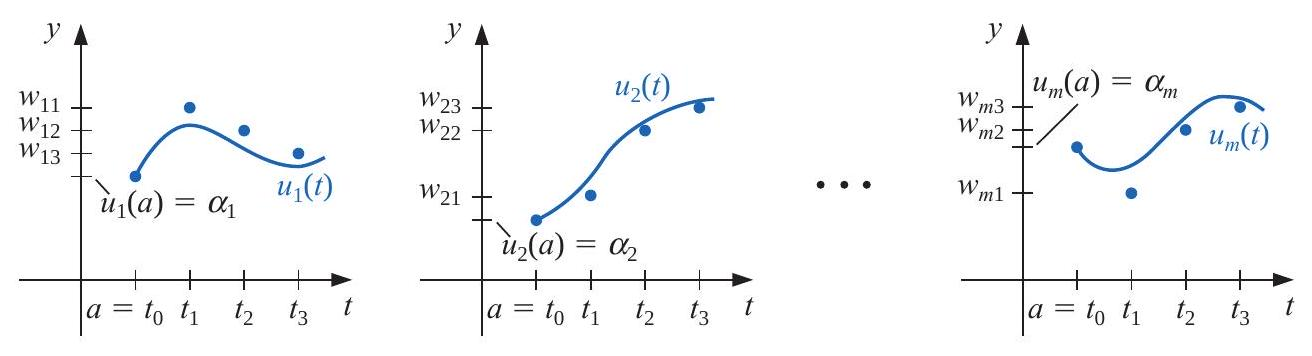
\includegraphics[width=14cmr]{2025_05_15_5266fa2c85d567bd073dg-72}
\caption{\scriptsize Figure $1$}
\label{fig:hoesdefig1}
\end{figure}

Suppose that the values $w_{1, j}, w_{2, j}, \ldots, w_{m, j}$ have been computed. We obtain $w_{1, j+1}$, $w_{2, j+1}, \ldots, w_{m, j+1}$ by first calculating


\begin{equation}\label{eqn:hoesdeeq5}
k_{1, i} =h f_{i}\left(t_{j}, w_{1, j}, w_{2, j}, \ldots, w_{m, j}\right), \quad \text { for each } i=1,2, \ldots, m 
\end{equation}

\begin{equation}\label{eqn:hoesdeeq6}
k_{2, i} =h f_{i}\left(t_{j}+\frac{h}{2}, w_{1, j}+\frac{1}{2} k_{1,1}, w_{2, j}+\frac{1}{2} k_{1,2}, \ldots, w_{m, j}+\frac{1}{2} k_{1, m}\right)
\end{equation}

for each $i=1,2, \ldots, m$;

\begin{equation}\label{eqn:hoesdeeq7}
k_{3, i}=h f_{i}\left(t_{j}+\frac{h}{2}, w_{1, j}+\frac{1}{2} k_{2,1}, w_{2, j}+\frac{1}{2} k_{2,2}, \ldots, w_{m, j}+\frac{1}{2} k_{2, m}\right) \tag{5.51}
\end{equation}

for each $i=1,2, \ldots, m$;

\begin{equation}\label{eqn:hoesdeeq8}
k_{4, i}=h f_{i}\left(t_{j}+h, w_{1, j}+k_{3,1}, w_{2, j}+k_{3,2}, \ldots, w_{m, j}+k_{3, m}\right)
\end{equation}

for each $i=1,2, \ldots, m$; and then

\begin{equation}\label{eqn:hoesdeeq9}
w_{i, j+1}=w_{i, j}+\frac{1}{6}\left(k_{1, i}+2 k_{2, i}+2 k_{3, i}+k_{4, i}\right)
\end{equation}

for each $i=1,2, \ldots, m$. Note that all the values $k_{1,1}, k_{1,2}, \ldots, k_{1, m}$ must be computed before any of the terms of the form $k_{2, i}$ can be determined. In general, each $k_{l, 1}, k_{l, 2}, \ldots, k_{l, m}$ must be computed before any of the expressions $k_{l+1, i}$.
%
%\section*{Runge-Kutta Method for Systems of Differential Equations}
%To approximate the solution of the $m$ th-order system of first-order initial-value problems
%
%$$
%u_{j}^{\prime}=f_{j}\left(t, u_{1}, u_{2}, \ldots, u_{m}\right), \quad a \leq t \leq b, \quad \text { with } \quad u_{j}(a)=\alpha_{j},
%$$
%
%for $j=1,2, \ldots, m$ at ( $N+1$ ) equally spaced numbers in the interval $[a, b]$ :
%
%INPUT endpoints $a, b$; number of equations $m$; integer $N$; initial conditions $\alpha_{1}, \ldots, \alpha_{m}$. OUTPUT approximations $w_{j}$ to $u_{j}(t)$ at the $(N+1)$ values of $t$.
%
%Step 1 Set $h=(b-a) / N$;
%
%$$
%t=a .
%$$
%
%Step 2 For $j=1,2, \ldots, m$ set $w_{j}=\alpha_{j}$.\\
%Step 3 OUTPUT $\left(t, w_{1}, w_{2}, \ldots, w_{m}\right)$.\\
%Step 4 For $i=1,2, \ldots, N$ do steps 5-11.\\
%Step 5 For $j=1,2, \ldots, m$ set
%
%$$
%k_{1, j}=h f_{j}\left(t, w_{1}, w_{2}, \ldots, w_{m}\right)
%$$
%
%Step 6 For $j=1,2, \ldots, m$ set
%
%$$
%k_{2, j}=h f_{j}\left(t+\frac{h}{2}, w_{1}+\frac{1}{2} k_{1,1}, w_{2}+\frac{1}{2} k_{1,2}, \ldots, w_{m}+\frac{1}{2} k_{1, m}\right) .
%$$
%
%Step 7 For $j=1,2, \ldots, m$ set
%
%$$
%k_{3, j}=h f_{j}\left(t+\frac{h}{2}, w_{1}+\frac{1}{2} k_{2,1}, w_{2}+\frac{1}{2} k_{2,2}, \ldots, w_{m}+\frac{1}{2} k_{2, m}\right) .
%$$
%
%Step 8 For $j=1,2, \ldots, m$ set
%
%$$
%k_{4, j}=h f_{j}\left(t+h, w_{1}+k_{3,1}, w_{2}+k_{3,2}, \ldots, w_{m}+k_{3, m}\right) .
%$$
%
%Step 9 For $j=1,2, \ldots, m$ set
%
%$$
%w_{j}=w_{j}+\left(k_{1, j}+2 k_{2, j}+2 k_{3, j}+k_{4, j}\right) / 6
%$$
%
%Step 10 Set $t=a+i h$.\\
%Step 11 OUTPUT $\left(t, w_{1}, w_{2}, \ldots, w_{m}\right)$.
%
%\section*{Step 12 STOP.}

\begin{example}
 Kirchhoff's Law states that the sum of all instantaneous voltage changes around a closed circuit is zero. This law implies that the current $I(t)$ in a closed circuit containing a resistance of $R$ ohms, a capacitance of $C$ farads, an inductance of $L$ henries, and a voltage source of $E(t)$ volts satisfies the equation

$$
L I^{\prime}(t)+R I(t)+\frac{1}{C} \int I(t) d t=E(t)
$$

The currents $I_{1}(t)$ and $I_{2}(t)$ in the left and right loops, respectively, of the circuit shown in Figure \ref{fig:hoesdefig2} are the solutions to the system of equations

$$
\begin{aligned}
2 I_{1}(t)+6\left[I_{1}(t)-I_{2}(t)\right]+2 I_{1}^{\prime}(t) & =12 \\
\frac{1}{0.5} \int I_{2}(t) d t+4 I_{2}(t)+6\left[I_{2}(t)-I_{1}(t)\right] & =0
\end{aligned}
$$

If the switch in the circuit is closed at time $t=0$, we have the initial conditions $I_{1}(0)=0$ and $I_{2}(0)=0$. Solve for $I_{1}^{\prime}(t)$ in the first equation, differentiate the second equation, and substitute for $I_{1}^{\prime}(t)$ to get

$$
\begin{aligned}
& I_{1}^{\prime}=f_{1}\left(t, I_{1}, I_{2}\right)=-4 I_{1}+3 I_{2}+6, \quad I_{1}(0)=0 \\
& I_{2}^{\prime}=f_{2}\left(t, I_{1}, I_{2}\right)=0.6 I_{1}^{\prime}-0.2 I_{2}=-2.4 I_{1}+1.6 I_{2}+3.6, \quad I_{2}(0)=0
\end{aligned}
$$

The exact solution to this system is

$$
\begin{aligned}
& I_{1}(t)=-3.375 e^{-2 t}+1.875 e^{-0.4 t}+1.5 \\
& I_{2}(t)=-2.25 e^{-2 t}+2.25 e^{-0.4 t}
\end{aligned}
$$

We will apply the Runge-Kutta method of order four to this system with $h=0.1$. Since $w_{1,0}=I_{1}(0)=0$ and $w_{2,0}=I_{2}(0)=0$,

$$
\begin{aligned}
k_{1,1} & =h f_{1}\left(t_{0}, w_{1,0}, w_{2,0}\right)=0.1 f_{1}(0,0,0)=0.1(-4(0)+3(0)+6)=0.6 \\
k_{1,2} & =h f_{2}\left(t_{0}, w_{1,0}, w_{2,0}\right)=0.1 f_{2}(0,0,0)=0.1(-2.4(0)+1.6(0)+3.6)=0.36 \\
k_{2,1} & =h f_{1}\left(t_{0}+\frac{1}{2} h, w_{1,0}+\frac{1}{2} k_{1,1}, w_{2,0}+\frac{1}{2} k_{1,2}\right)=0.1 f_{1}(0.05,0.3,0.18) \\
& =0.1(-4(0.3)+3(0.18)+6)=0.534 \\
k_{2,2} & =h f_{2}\left(t_{0}+\frac{1}{2} h, w_{1,0}+\frac{1}{2} k_{1,1}, w_{2,0}+\frac{1}{2} k_{1,2}\right)=0.1 f_{2}(0.05,0.3,0.18) \\
& =0.1(-2.4(0.3)+1.6(0.18)+3.6)=0.3168
\end{aligned}
$$

Generating the remaining entries in a similar manner produces

$$
\begin{aligned}
& k_{3,1}=(0.1) f_{1}(0.05,0.267,0.1584)=0.54072 \\
& k_{3,2}=(0.1) f_{2}(0.05,0.267,0.1584)=0.321264 \\
& k_{4,1}=(0.1) f_{1}(0.1,0.54072,0.321264)=0.4800912 \\
& k_{4,2}=(0.1) f_{2}(0.1,0.54072,0.321264)=0.28162944
\end{aligned}
$$

As a consequence,

$$
\begin{aligned}
I_{1}(0.1) \approx w_{1,1} & =w_{1,0}+\frac{1}{6}\left(k_{1,1}+2 k_{2,1}+2 k_{3,1}+k_{4,1}\right) \\
& =0+\frac{1}{6}(0.6+2(0.534)+2(0.54072)+0.4800912)=0.5382552
\end{aligned}
$$

and

$$
I_{2}(0.1) \approx w_{2,1}=w_{2,0}+\frac{1}{6}\left(k_{1,2}+2 k_{2,2}+2 k_{3,2}+k_{4,2}\right)=0.3196263
$$

The remaining entries in Table \ref{tab:hoesdetab1} are generated in a similar manner.
\end{example}

%Figure 5.7\\
\begin{figure}[h]
\centering
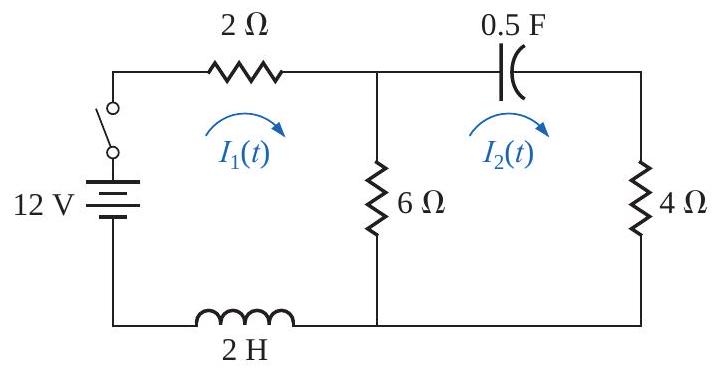
\includegraphics[width=9cm]{2025_05_15_5266fa2c85d567bd073dg-74}
\caption{\scriptsize Figure $2$}
\label{fig:hoesdefig2}
\end{figure}


%Table 5.19

\begin{table}[h]
\centering
\begin{tabular}{|l|l|l|l|l|}
\hline
$t_{j}$ & $w_{1, j}$ & $w_{2, j}$ & $\left|I_{1}\left(t_{j}\right)-w_{1, j}\right|$ & $\left|I_{2}\left(t_{j}\right)-w_{2, j}\right|$ \\
\hline
0.0 & 0 & 0 & 0 & 0 \\
\hline
0.1 & 0.5382550 & 0.3196263 & $0.8285 \times 10^{-5}$ & $0.5803 \times 10^{-5}$ \\
\hline
0.2 & 0.9684983 & 0.5687817 & $0.1514 \times 10^{-4}$ & $0.9596 \times 10^{-5}$ \\
\hline
0.3 & 1.310717 & 0.7607328 & $0.1907 \times 10^{-4}$ & $0.1216 \times 10^{-4}$ \\
\hline
0.4 & 1.581263 & 0.9063208 & $0.2098 \times 10^{-4}$ & $0.1311 \times 10^{-4}$ \\
\hline
0.5 & 1.793505 & 1.014402 & $0.2193 \times 10^{-4}$ & $0.1240 \times 10^{-4}$ \\
\hline
\end{tabular}
\caption{\scriptsize Table $4$}
\label{tab:hoesdetab1}
\end{table}

%Recall that Maple reserves the letter $D$ to represent differentiation.
%
%Maple's NumericalAnalysis package does not currently approximate the solution to systems of initial value problems, but systems of first-order differential equations can by solved using dsolve. The system in the Illustration is defined with\\
%sys $2:=D(u 1)(t)=-4 u 1(t)+3 u 2(t)+6, D(u 2)(t)=-2.4 u 1(t)+1.6 u 2(t)+3.6$\\
%and the initial conditions with\\
%init $2:=u 1(0)=0, u 2(0)=0$\\
%The system is solved with the command\\
%sol $2:=$ dsolve $(\{$ sys 2, init 2$\},\{u 1(t), u 2(t)\})$\\
%and Maple responds with
%
%$$
%\left\{u 1(t)=-\frac{27}{8} e^{-2 t}+\frac{15}{8} e^{-\frac{5}{2} t}+\frac{3}{2}, u 2(t)=-\frac{9}{4} e^{-2 t}+\frac{9}{4} e^{-\frac{5}{2} t}\right\}
%$$
%
%To isolate the individual functions we use\\
%$r 1:=\operatorname{rhs}(\operatorname{sol} 2[1]) ; r 2:=\operatorname{rhs}(\operatorname{sol} 2[2])$\\
%producing
%
%$$
%\begin{aligned}
%& -\frac{27}{8} e^{-2 t}+\frac{15}{8} e^{-\frac{5}{2} t}+\frac{3}{2} \\
%& -\frac{9}{4} e^{-2 t}+\frac{9}{4} e^{-\frac{5}{2} t}
%\end{aligned}
%$$
%
%and to determine the value of the functions at $t=0.5$ we use\\
%$\operatorname{evalf}(\operatorname{subs}(t=0.5, r 1)) ; \operatorname{evalf}(\operatorname{subs}(t=0.5, r 2))$\\
%giving, in agreement with Table 5.19,\\
%1.793527048\\
%1.014415451
%
%The command dsolve will fail if an explicit solution cannot be found. In that case we can use the numeric option in dsolve, which applies the Runge-Kutta-Fehlberg technique. This technique can also be used, of course, when the exact solution can be determined with dsolve. For example, with the system defined previously,\\
%$g:=$ dsolve (\{sys 2, init 2\}, \{ $u 1(t), u 2(t)\}$, numeric)\\
%returns
%
%$$
%\operatorname{proc}\left(x_{-} r k f 45\right) \ldots \text { end proc }
%$$
%
%To approximate the solutions at $t=0.5$, enter\\
%$g(0.5)$\\
%which gives approximations in the form
%
%$$
%[t=0.5, u 2(t)=1.014415563, u 1(t)=1.793527215]
%$$
%
\subsection*{Higher-Order Differential Equations}
%Many important physical problems-for example, electrical circuits and vibrating systemsinvolve initial-value problems whose equations have orders higher than one. New techniques are not required for solving these problems. By relabeling the variables, we can reduce a higher-order differential equation into a system of first-order differential equations and then apply one of the methods we have already discussed.

A general $m$ th-order initial-value problem

$$
y^{(m)}(t)=f\left(t, y, y^{\prime}, \ldots, y^{(m-1)}\right), \quad a \leq t \leq b
$$

with initial conditions $y(a)=\alpha_{1}, y^{\prime}(a)=\alpha_{2}, \ldots, y^{(m-1)}(a)=\alpha_{m}$ can be converted into a system of equations in the form (5.45) and (5.46).

Let $u_{1}(t)=y(t), u_{2}(t)=y^{\prime}(t), \ldots$, and $u_{m}(t)=y^{(m-1)}(t)$. This produces the first-order system

$$
\frac{d u_{1}}{d t}=\frac{d y}{d t}=u_{2}, \quad \frac{d u_{2}}{d t}=\frac{d y^{\prime}}{d t}=u_{3}, \quad \cdots, \quad \frac{d u_{m-1}}{d t}=\frac{d y^{(m-2)}}{d t}=u_{m}
$$

and

$$
\frac{d u_{m}}{d t}=\frac{d y^{(m-1)}}{d t}=y^{(m)}=f\left(t, y, y^{\prime}, \ldots, y^{(m-1)}\right)=f\left(t, u_{1}, u_{2}, \ldots, u_{m}\right)
$$

with initial conditions

$$
u_{1}(a)=y(a)=\alpha_{1}, \quad u_{2}(a)=y^{\prime}(a)=\alpha_{2}, \quad \ldots, \quad u_{m}(a)=y^{(m-1)}(a)=\alpha_{m}
$$

\begin{example}
Transform the the second-order initial-value problem

$$
y^{\prime \prime}-2 y^{\prime}+2 y=e^{2 t} \sin t, \quad \text { for } 0 \leq t \leq 1, \quad \text { with } y(0)=-0.4, y^{\prime}(0)=-0.6
$$

into a system of first order initial-value problems, and use the Runge-Kutta method with $h=0.1$ to approximate the solution.
\end{example}

\begin{mysolution}
Let $u_{1}(t)=y(t)$ and $u_{2}(t)=y^{\prime}(t)$. This transforms the second-order equation into the system

$$
\begin{aligned}
& u_{1}^{\prime}(t)=u_{2}(t) \\
& u_{2}^{\prime}(t)=e^{2 t} \sin t-2 u_{1}(t)+2 u_{2}(t)
\end{aligned}
$$

with initial conditions $u_{1}(0)=-0.4, u_{2}(0)=-0.6$.\\
The initial conditions give $w_{1,0}=-0.4$ and $w_{2,0}=-0.6$. The Runge-Kutta Eqs. (5.49) through (5.52) on page 330 with $j=0$ give

$$
\begin{aligned}
k_{1,1} & =h f_{1}\left(t_{0}, w_{1,0}, w_{2,0}\right)=h w_{2,0}=-0.06 \\
k_{1,2} & =h f_{2}\left(t_{0}, w_{1,0}, w_{2,0}\right)=h\left[e^{2 t_{0}} \sin t_{0}-2 w_{1,0}+2 w_{2,0}\right]=-0.04 \\
k_{2,1} & =h f_{1}\left(t_{0}+\frac{h}{2}, w_{1,0}+\frac{1}{2} k_{1,1}, w_{2,0}+\frac{1}{2} k_{1,2}\right)=h\left[w_{2,0}+\frac{1}{2} k_{1,2}\right]=-0.062 \\
k_{2,2} & =h f_{2}\left(t_{0}+\frac{h}{2}, w_{1,0}+\frac{1}{2} k_{1,1}, w_{2,0}+\frac{1}{2} k_{1,2}\right) \\
& =h\left[e^{2\left(t_{0}+0.05\right)} \sin \left(t_{0}+0.05\right)-2\left(w_{1,0}+\frac{1}{2} k_{1,1}\right)+2\left(w_{2,0}+\frac{1}{2} k_{1,2}\right)\right] \\
& =-0.03247644757 \\
k_{3,1} & =h\left[w_{2,0}+\frac{1}{2} k_{2,2}\right]=-0.06162832238 \\
k_{3,2} & =h\left[e^{2\left(t_{0}+0.05\right)} \sin \left(t_{0}+0.05\right)-2\left(w_{1,0}+\frac{1}{2} k_{2,1}\right)+2\left(w_{2,0}+\frac{1}{2} k_{2,2}\right)\right] \\
& =-0.03152409237 \\
k_{4,1} & =h\left[w_{2,0}+k_{3,2}\right]=-0.06315240924
\end{aligned}
$$

and

$$
k_{4,2}=h\left[e^{2\left(t_{0}+0.1\right)} \sin \left(t_{0}+0.1\right)-2\left(w_{1,0}+k_{3,1}\right)+2\left(w_{2,0}+k_{3,2}\right)\right]=-0.02178637298
$$

So

$$
w_{1,1}=w_{1,0}+\frac{1}{6}\left(k_{1,1}+2 k_{2,1}+2 k_{3,1}+k_{4,1}\right)=-0.4617333423
$$

and

$$
w_{2,1}=w_{2,0}+\frac{1}{6}\left(k_{1,2}+2 k_{2,2}+2 k_{3,2}+k_{4,2}\right)=-0.6316312421
$$

The value $w_{1,1}$ approximates $u_{1}(0.1)=y(0.1)=0.2 e^{2(0.1)}(\sin 0.1-2 \cos 0.1)$, and $w_{2,1}$ approximates $u_{2}(0.1)=y^{\prime}(0.1)=0.2 e^{2(0.1)}(4 \sin 0.1-3 \cos 0.1)$.

The set of values $w_{1, j}$ and $w_{2, j}$, for $j=0,1, \ldots, 10$, are presented in Table \ref{tab:hoesdetab1} and are compared to the actual values of $u_{1}(t)=0.2 e^{2 t}(\sin t-2 \cos t)$ and $u_{2}(t)=u_{1}^{\prime}(t)=$ $0.2 e^{2 t}(4 \sin t-3 \cos t)$.
\end{mysolution}
%Table 5.20

\begin{table}[h]
\centering
\begin{tabular}{|l|l|l|l|l|l|l|}
\hline
$t_{j}$ & $y\left(t_{j}\right)=u_{1}\left(t_{j}\right)$ & $w_{1, j}$ & $y^{\prime}\left(t_{j}\right)=u_{2}\left(t_{j}\right)$ & $w_{2, j}$ & $\left|y\left(t_{j}\right)-w_{1, j}\right|$ & $\left|y^{\prime}\left(t_{j}\right)-w_{2, j}\right|$ \\
\hline
0.0 & -0.40000000 & -0.40000000 & -0.6000000 & -0.60000000 & 0 & 0 \\
\hline
0.1 & -0.46173297 & -0.46173334 & -0.6316304 & -0.63163124 & $3.7 \times 10^{-7}$ & $7.75 \times 10^{-7}$ \\
\hline
0.2 & -0.52555905 & -0.52555988 & -0.6401478 & -0.64014895 & $8.3 \times 10^{-7}$ & $1.01 \times 10^{-6}$ \\
\hline
0.3 & -0.58860005 & -0.58860144 & -0.6136630 & -0.61366381 & $1.39 \times 10^{-6}$ & $8.34 \times 10^{-7}$ \\
\hline
0.4 & -0.64661028 & -0.64661231 & -0.5365821 & -0.53658203 & $2.03 \times 10^{-6}$ & $1.79 \times 10^{-7}$ \\
\hline
0.5 & -0.69356395 & -0.69356666 & -0.3887395 & -0.38873810 & $2.71 \times 10^{-6}$ & $5.96 \times 10^{-7}$ \\
\hline
0.6 & -0.72114849 & -0.72115190 & -0.1443834 & -0.14438087 & $3.41 \times 10^{-6}$ & $7.75 \times 10^{-7}$ \\
\hline
0.7 & -0.71814890 & -0.71815295 & 0.2289917 & 0.22899702 & $4.05 \times 10^{-6}$ & $2.03 \times 10^{-6}$ \\
\hline
0.8 & -0.66970677 & -0.66971133 & 0.7719815 & 0.77199180 & $4.56 \times 10^{-6}$ & $5.30 \times 10^{-6}$ \\
\hline
0.9 & -0.55643814 & -0.55644290 & 1.534764 & 1.5347815 & $4.76 \times 10^{-6}$ & $9.54 \times 10^{-6}$ \\
\hline
1.0 & -0.35339436 & -0.35339886 & 2.578741 & 2.5787663 & $4.50 \times 10^{-6}$ & $1.34 \times 10^{-5}$ \\
\hline
\end{tabular}
\caption{\scriptsize Table $5$}
\label{tab:hoesdetab2}
\end{table}

%In Maple the $n$th derivative $y^{(n)}(t)$ is specified by $(D @ @ n)(y)(t)$.
%
%We can also use dsolve from Maple on higher-order equations. To define the differential equation in Example 1, use\\
%$\operatorname{def} 2:=(D @ @ 2)(y)(t)-2 D(y)(t)+2 y(t)=e^{2 t} \sin (t)$\\
%and to specify the initial conditions use\\
%init $2:=y(0)=-0.4, D(y)(0)=-0.6$\\
%The solution is obtained with the command\\
%sol $2:=$ dsolve $(\{$ def 2, init 2$\}, y(t))$\\
%to obtain
%
%$$
%y(t)=\frac{1}{5} e^{2 t}(\sin (t)-2 \cos (t))
%$$
%
%We isolate the solution in function form using\\
%$g:=\operatorname{rhs}(\operatorname{sol} 2)$\\
%To obtain $y(1.0)=g(1.0)$, enter\\
%$\operatorname{evalf}(\operatorname{subs}(t=1.0, g))$\\
%which gives -0.3533943574 .\\
Runge-Kutta-Fehlberg is also available for higher-order equations via the dsolve command with the numeric option. It is employed in the same manner as illustrated for systems of equations.

The other one-step methods can be extended to systems in a similar way. When error control methods like the Runge-Kutta-Fehlberg method are extended, each component of the numerical solution $\left(w_{1 j}, w_{2 j}, \ldots, w_{m j}\right)$ must be examined for accuracy. If any of the components fail to be sufficiently accurate, the entire numerical solution $\left(w_{1 j}, w_{2 j}, \ldots, w_{m j}\right)$ must be recomputed.

The multistep methods and predictor-corrector techniques can also be extended to systems. Again, if error control is used, each component must be accurate. The extension of the extrapolation technique to systems can also be done, but the notation becomes quite involved. 

%Convergence theorems and error estimates for systems are similar to those considered in Section 5.10 for the single equations, except that the bounds are given in terms of vector norms, a topic considered in Chapter 7. (A good reference for these theorems is [Ge1], pp. 45-72.)

\begin{myexercise}%\label{Comprehensionquiz2}
Use the Runge-Kutta for Systems Algorithm to approximate the solutions of the following higher order differential equations, and compare the results to the actual solutions.
\begin{enumerate}[label=(\alph*)]
\item $y^{\prime \prime}-2 y^{\prime}+y=t e^{t}-t$, $0 \leq t \leq 1$, $y(0)=y^{\prime}(0)=0$, with $h=0.1$;
actual solution $y(t)=\frac{1}{6} t^{3} e^{t}-t e^{t}+2 e^{t}-t-2$.\\
\item $t^{2} y^{\prime \prime}-2 t y^{\prime}+2 y=t^{3} \ln t$, $1 \leq t \leq 2, \quad y(1)=1$, $y^{\prime}(1)=0$, with $h=0.1$; actual solution $y(t)=\frac{7}{4} t+\frac{1}{2} t^{3} \ln t-\frac{3}{4} t^{3}$.
%\item $y^{\prime \prime \prime}+2 y^{\prime \prime}-y^{\prime}-2 y=e^{t}$, $0 \leq t \leq 3, \quad y(0)=1$, $y^{\prime}(0)=2$, $y^{\prime \prime}(0)=0$, with $h=0.2$; actual solution $y(t)=\frac{43}{36} e^{t}+\frac{1}{4} e^{-t}-\frac{4}{9} e^{-2 t}+\frac{1}{6} t e^{t}$.\\
%\item $t^{3} y^{\prime \prime \prime}-t^{2} y^{\prime \prime}+3 t y^{\prime}-4 y=5 t^{3} \ln t+9 t^{3}$, $1 \leq t \leq 2$, $y(1)=0, \quad y^{\prime}(1)=1$, $y^{\prime \prime}(1)=3$, with $h=0.1$; actual solution $y(t)=-t^{2}+t \cos (\ln t)+t \sin (\ln t)+t^{3} \ln t$.
\end{enumerate}

\begin{mysolution}
The Runge-Kutta for Systems Algorithm gives the results in the following tables.\\
\begin{enumerate}[label=(\alph*).]
\item

\begin{center}
\begin{tabular}{ccc}
\hline
$t_{i}$ & $w_{1 i}$ & $y_{i}$ \\
\hline
0.200 & 0.00015352 & 0.00015350 \\
0.500 & 0.00742968 & 0.00743027 \\
0.700 & 0.03299617 & 0.03299805 \\
1.000 & 0.17132224 & 0.17132880 \\
\hline
\end{tabular}
\end{center}

\item
\begin{center}
\begin{tabular}{ccc}
\hline
$t_{i}$ & $w_{1 i}$ & $y_{i}$ \\
\hline
1.200 & 0.96152437 & 0.96152583 \\
1.500 & 0.77796897 & 0.77797237 \\
1.700 & 0.59373369 & 0.59373830 \\
2.000 & 0.27258237 & 0.27258872 \\
\end{tabular}
\end{center}


%\item
%
%\begin{center}
%\begin{tabular}{ccc}
%\hline
%$t_{i}$ & $w_{1 i}$ & $y_{i}$ \\
%\hline
%1.000 & 3.73162695 & 3.73170445 \\
%2.000 & 11.31424573 & 11.31452924 \\
%3.000 & 34.04395688 & 34.04517155 \\
%\hline
%\end{tabular}
%\end{center}
%
%\item
%
%\begin{center}
%\begin{tabular}{ccc}
%\hline
%$t_{i}$ & $w_{1 i}$ & $w_{2 i}$ \\
%\hline
%1.200 & 0.27273759 & 0.27273791 \\
%1.500 & 1.08849079 & 1.08849259 \\
%1.700 & 2.04353207 & 2.04353642 \\
%2.000 & 4.36156675 & 4.36157780 \\
%\hline
%\end{tabular}
%\end{center}

\end{enumerate}
\end{mysolution}
\end{myexercise}





\section{Stability and Stiff Differential Equations}
%\videolesson
%\begin{selfvideo}[2]
%%LESSON 3: 
%This video presents a discussion on stability and stiff differential equations. Follow the discussion and then solve the problems in the subsequent quiz.
%\end{selfvideo}
%\begin{boxB}Question: \end{boxB}

\begin{youtube}
This video presents a discussion on stability and stiff differential equations. Follow the discussion and then solve the problems in the subsequent quiz.
\end{youtube}

\mylink{https://www.youtube.com/watch?\\v=yABmV2qnzcg\&list=PLkiPLxr5Ckwsk1A\_qK\_AK\_8LGFoxqdox2\&index=5}

\mylink{https://www.youtube.com/watch?v=-YoojEp24BA}

\mylink{https://www.youtube.com/watch?v=lQENz3-HOLQ}

\mylink{https://www.youtube.com/watch?v=C72rIeiv7mg}
\begin{myexercise}%\label{Comprehensionquiz2}
Given the multistep method

$$
w_{i+1}=-\frac{3}{2} w_{i}+3 w_{i-1}-\frac{1}{2} w_{i-2}+3 h f\left(t_{i}, w_{i}\right), \quad \text { for } i=2, \ldots, N-1,
$$

with starting values $w_{0}, w_{1}, w_{2}$ :
\begin{enumerate}[label=(\alph*)]
\item  Find the local truncation error.
\item Comment on consistency, stability, and convergence.
\end{enumerate}

\begin{mysolution}


\begin{enumerate}[label=(\alph*)]
\item The local truncation error is $\tau_{i+1}=\frac{1}{4} h^{3} y^{(4)}\left(\xi_{i}\right)$, for some $\xi$, where $t_{i-2}<\xi_{i}<t_{i+1}$.\\
\item The method is consistent but unstable and not convergent.
\end{enumerate}
\end{mysolution}
\end{myexercise}


%\discussion


\begin{posttest}%[\textcolor{red}{End of Module 8 Quiz}]
\item An electrical circuit consists of a capacitor of constant capacitance $C=1.1$ farads in series with a resistor of constant resistance $R_{0}=2.1$ ohms. A voltage $\mathcal{E}(t)=110 \sin t$ is applied at time $t=0$. When the resistor heats up, the resistance becomes a function of the current $i$,


$$
R(t)=R_{0}+k i, \quad \text { where } k=0.9
$$

and the differential equation for $i(t)$ becomes

$$
\left(1+\frac{2 k}{R_{0}} i\right) \frac{d i}{d t}+\frac{1}{R_{0} C} i=\frac{1}{R_{0} C} \frac{d \mathcal{E}}{d t}
$$

Find $i(2)$, assuming that $i(0)=0$. 


\item Use the Extrapolation Algorithm with tolerance $T O L=10^{-6}, h \max =0.5$, and $h \min =0.05$ to approximate the solutions to the following initial-value problems. Compare the results to the actual values.
\begin{enumerate}[label=(\alph*)]
  \item $\quad y^{\prime}=y / t-(y / t)^{2}, \quad 1 \leq t \leq 4, \quad y(1)=1$; actual solution $y(t)=t /(1+\ln t)$.\\
\item $\quad y^{\prime}=1+y / t+(y / t)^{2}, \quad 1 \leq t \leq 3, \quad y(1)=0$; actual solution $y(t)=t \tan (\ln t)$.
\end{enumerate}

\item Use the Runge-Kutta for Systems Algorithm to approximate the solutions of the following higher order differential equations, and compare the results to the actual solutions.
\begin{enumerate}[label=(\alph*)]
%\item $y^{\prime \prime}-2 y^{\prime}+y=t e^{t}-t$, $0 \leq t \leq 1$, $y(0)=y^{\prime}(0)=0$, with $h=0.1$;
%actual solution $y(t)=\frac{1}{6} t^{3} e^{t}-t e^{t}+2 e^{t}-t-2$.\\
%\item $t^{2} y^{\prime \prime}-2 t y^{\prime}+2 y=t^{3} \ln t$, $1 \leq t \leq 2, \quad y(1)=1$, $y^{\prime}(1)=0$, with $h=0.1$; actual solution $y(t)=\frac{7}{4} t+\frac{1}{2} t^{3} \ln t-\frac{3}{4} t^{3}$.\\
\item $y^{\prime \prime \prime}+2 y^{\prime \prime}-y^{\prime}-2 y=e^{t}$, $0 \leq t \leq 3, \quad y(0)=1$, $y^{\prime}(0)=2$, $y^{\prime \prime}(0)=0$, with $h=0.2$; actual solution $y(t)=\frac{43}{36} e^{t}+\frac{1}{4} e^{-t}-\frac{4}{9} e^{-2 t}+\frac{1}{6} t e^{t}$.\\
\item $t^{3} y^{\prime \prime \prime}-t^{2} y^{\prime \prime}+3 t y^{\prime}-4 y=5 t^{3} \ln t+9 t^{3}$, $1 \leq t \leq 2$, $y(1)=0, \quad y^{\prime}(1)=1$, $y^{\prime \prime}(1)=3$, with $h=0.1$; actual solution $y(t)=-t^{2}+t \cos (\ln t)+t \sin (\ln t)+t^{3} \ln t$.
\end{enumerate}

\item Solve the following stiff initial-value problem using the Runge-Kutta fourth-order method with (a) $h=0.1$ and (b) $h=0.025$.


$$
\begin{aligned}
& u_{1}^{\prime}=32 u_{1}+66 u_{2}+\frac{2}{3} t+\frac{2}{3}, \quad 0 \leq t \leq 0.5, \quad u_{1}(0)=\frac{1}{3} \\
& u_{2}^{\prime}=-66 u_{1}-133 u_{2}-\frac{1}{3} t-\frac{1}{3}, \quad 0 \leq t \leq 0.5, \quad u_{2}(0)=\frac{1}{3}
\end{aligned}
$$

Compare the results to the actual solution,

$$
u_{1}(t)=\frac{2}{3} t+\frac{2}{3} e^{-t}-\frac{1}{3} e^{-100 t} \quad \text { and } \quad u_{2}(t)=-\frac{1}{3} t-\frac{1}{3} e^{-t}+\frac{2}{3} e^{-100 t}
$$

\begin{mysolution}
\begin{enumerate}[label=\arabic*.]
  \item The current after 2 seconds is approximately $i(2)=8.693$ amperes.

\item The Extrapolation Algorithm gives the results in the following tables.\\
\begin{enumerate}[label=(\alph*).]
\item

\begin{center}
\begin{tabular}{cccccc}
\hline
$i$ & $t_{i}$ & $w_{i}$ & $h$ & $k$ & $y_{i}$ \\
\hline
1 & 1.50 & 1.06726237 & 0.50 & 4 & 1.06726235 \\
2 & 2.00 & 1.18123223 & 0.50 & 3 & 1.18123222 \\
3 & 2.50 & 1.30460372 & 0.50 & 3 & 1.30460371 \\
4 & 3.00 & 1.42951608 & 0.50 & 3 & 1.42951607 \\
5 & 3.50 & 1.55364771 & 0.50 & 3 & 1.55364770 \\
6 & 4.00 & 1.67623915 & 0.50 & 3 & 1.67623914 \\
\hline
\end{tabular}
\end{center}

\item

\begin{center}
\begin{tabular}{cccccc}
\hline
$i$ & $t_{i}$ & $w_{i}$ & $h$ & $k$ & $y_{i}$ \\
\hline
1 & 1.50 & 0.64387537 & 0.50 & 4 & 0.64387533 \\
2 & 2.00 & 1.66128182 & 0.50 & 5 & 1.66128176 \\
3 & 2.50 & 3.25801550 & 0.50 & 5 & 3.25801536 \\
4 & 3.00 & 5.87410027 & 0.50 & 5 & 5.87409998 \\
\hline
\end{tabular}
\end{center}
\end{enumerate}

\vspace{5mm}
\item The Runge-Kutta for Systems Algorithm gives the results in the following tables.\\
\begin{enumerate}[label=(\alph*).]
\item

\begin{center}
\begin{tabular}{ccc}
\hline
$t_{i}$ & $w_{1 i}$ & $y_{i}$ \\
\hline
1.000 & 3.73162695 & 3.73170445 \\
2.000 & 11.31424573 & 11.31452924 \\
3.000 & 34.04395688 & 34.04517155 \\
\hline
\end{tabular}
\end{center}

\item

\begin{center}
\begin{tabular}{ccc}
\hline
$t_{i}$ & $w_{1 i}$ & $w_{2 i}$ \\
\hline
1.200 & 0.27273759 & 0.27273791 \\
1.500 & 1.08849079 & 1.08849259 \\
1.700 & 2.04353207 & 2.04353642 \\
2.000 & 4.36156675 & 4.36157780 \\
\hline
\end{tabular}
\end{center}

\end{enumerate}

\vspace{5mm}
\item 
\begin{enumerate}[label=(\alph*).]
\item
\begin{center}
\begin{tabular}{|l|l|l|l|l|}
\hline
$t_{i}$ & $w_{1 i}$ & $u_{1 i}$ & $w_{2 i}$ & $u_{2 i}$ \\
\hline
0.100 & -96.33011 & 0.66987648 & 193.6651 & -0.33491554 \\
\hline
0.200 & -28226.32 & 0.67915383 & 56453.66 & -0.33957692 \\
\hline
0.300 & -8214056 & 0.69387881 & 16428113 & -0.34693941 \\
\hline
0.400 & -2390290586 & 0.71354670 & 4780581173 & -0.35677335 \\
\hline
0.500 & -695574560790 & 0.73768711 & 1391149121600 & -0.36884355 \\
\hline
\end{tabular}
\end{center}

\item

\begin{center}
\begin{tabular}{ccccc}
\hline
$t_{i}$ & $w_{1 i}$ & $u_{1 i}$ & $w_{2 i}$ & $u_{2 i}$ \\
\hline
0.100 & 0.61095960 & 0.66987648 & -0.21708179 & -0.33491554 \\
0.200 & 0.66873489 & 0.67915383 & -0.31873903 & -0.33957692 \\
0.300 & 0.69203679 & 0.69387881 & -0.34325535 & -0.34693941 \\
0.400 & 0.71322103 & 0.71354670 & -0.35612202 & -0.35677335 \\
0.500 & 0.73762953 & 0.73768711 & -0.36872840 & -0.36884355 \\
\hline
\end{tabular}
\end{center}
\end{enumerate}
\end{enumerate}
\end{mysolution}
\end{posttest}

%share your understanding of properties of functions and their applications to solving rates of change problems in physical phenomenon 


%\end{actsoln}

\takehome

\comy{You are now at the last part of this module. Your  task is to do a self-reflection on your learning experience.}



\references
\begin{refenumerate}
\item Kong, Q., Siauw, T., Bayen, A., (2020). Python Programming and Numerical Methods. First Edition, Academic Press,  ISBN-13 ‏ : ‎ 978-0128195499 \\
\mylink{https://pythonnumericalmethods.studentorg.berkeley.edu/notebooks/Index.html}
%chapter 1 pg 7-36 functions\\
%chapter 1 pg 51-83 limits and continuity\\
%chapter 1 pg 45-50 rates of change\\
%chapter 2 pg 108-120 the derivative\\
%\item Mendelson, E. (2022). Schaum's Outline of Calculus. McGraw-Hill Education.
%chapter 6 51-55 functions
%chapter 7 59-65 limits
%chapter 8 69-74 continuity
%chapter 9 77-81 derivative
%\item Calculus \mylink{https://math.libretexts.org/Bookshelves/Calculus}
%\item Chris McMullen, 2021, Essential Calculus Skills Practice Workbook with Full Solutions, Zishka Publishing, ISBN 978-1-941691-24-3
%\item R. Adams and C. Essex, 2021, Calculus: A complete Course, Addison Wesley, ISBN 13: 978-0135732588
%\item P. Abbott and H. Neill, 2018, Calculus: A Complete Introduction: The Easy Way to Learn Calculus (Teach Yourself), ISBN 13: 978-1473678446
\end{refenumerate}





%\wrapup
%To wrap-up, answer the following questions:
%
%\begin{enumerate}
%\item 
%%when do we say that a limit of a function exists?
%%\item how do we remove discontinuity in functions?
%%\item what is the relationship between the gradient of the tangent line and the derivative?
%\end{enumerate}
















%\newpage

%\facilitation


%
\begin{center}
    {\Large \textbf{FUNCTIONS OF SEVERAL VARIABLES}}\\[2mm]
(DEFINITION, DOMAIN, RANGE, GRAPHS AND LEVEL CURVES) \\[4mm]

\mycenterbox{5 minute review}%\\[4mm]
Recap the definition of a function of several variables, and the meaning of domain, range, graph and level curves of functions of several variables.
\end{center}
\mycenterbox{Warm-up.}%\\[4mm]
\problemAnswer{
Match the function with its graph (labeled I–VI).Give reasons for your choices
\begin{multicols}{3}
\begin{enumerate}[label=(\alph*)]
\item $f(x,y)=|x|+|y|$\\[4mm]
\item $f(x,y)=|xy|$
\item $f(x,y)=\frac{1}{1+x^2+y^2}$\\2mm]
\item $f(x,y)=(x^2-y^2)^2$
\item $f(x,y)=(x-y)^2$\\[4mm]
\item $f(x,y)=\sin(|x|+|y|)$
\end{enumerate}
\end{multicols}

\begin{center}
%\centering
\includegraphics[width=10cm]{MCTutorial1Q1.JPEG}
\end{center}
%\tcbox[tcbox raise base]{Warm-up}
 
%\begin{flushright}
%\begin{tikzpicture}
%    % A body
%
%
%    % Non-rectangle shapes must be drawn as polygone
%    \begin{scope}[shift={(3,0)}]
%        \draw  (0,0.5) -- (0,4) -- (.5,4) -- (.5,4.5) -- (1.,4.5) -- (4.,4.5) --(4.,4)-- (4.5,4) --(4.5,0.5) --(4.0,0.5)--(4.0,0.0)-- (.5,0) --(0.5,0.5) -- cycle;
%        % Draw symmetry lines
%        \draw [symmetry] (.5, 0.5) -- (.5,4.0);
%        \draw [symmetry] (4, 0.5) -- (4,4.0);
%        \draw [symmetry] (.5,4.0) -- (4,4.0);
%         \draw [symmetry] (.5, 0.5) -- (4, 0.5);
%        % Dimensions
%        \draw (4.5,0) -- ++(0.5,0) coordinate (D1) -- +(5pt,0);
%        \draw (4.5,4.5) -- ++(0.5,0) coordinate (D2) -- +(5pt,0);
%        \draw [dimen] (D1) -- (D2) node {6cm};
%       
%        
%        \draw (0.0,5) -- ++(0,0.5) coordinate (D1) -- +(0,+5pt);
%        \draw (0.5,5) -- ++(0,0.5) coordinate (D2) -- +(0,+5pt);
%        \draw [dimen,-] (D1) -- (D2) node [above=5pt] {$x$ cm};
%        \draw [dimen,<-] (D1) -- ++(-5pt,0);
%        \draw [dimen,<-] (D2) -- ++(+5pt,0);
%    \end{scope}
%\end{tikzpicture}
%\end{flushright}

}


\mycenterbox{Problems.}%

%\begin{center}
%\tcbox[tcbox raise base]{ Problems. Choose from the below}
%\end{center}
\problem{Exploring functions}%
\begin{enumerate}[(a)]
\item Are the following functions even, odd, or neither? What can you say
about their range?
\begin{multicols}{4}
 \begin{enumerate}[(i)]
\item $\displaystyle \frac{3x}{x^2+2}$
\item $\displaystyle \cos x+3$
\item $\displaystyle \frac{2x^3}{\cos x+3}$
\item $\displaystyle \frac{3x^4+2x^2}{\sin x+4}$
\end{enumerate}
\end{multicols}
\item Consider the functions $\sin^n x$ and $\cos^n x$, where $n$ is a positive integer.
Which are odd, which are even, and what are their periodicities?
\item What is the periodicity of $f(x) = 2 \cos x+\sin 2x$? Is it even/odd/neither?

\end{enumerate}

\problem{Cubic functions} 
Show that $x-1$ is a factor of the cubic function%
$$P(x)=x^3-2x^2-5x+6,$$
and  find the quadratic factor $Q(x)$ such that $P(x) = (x -1)Q(x)$. Factorise
$Q(x)$ and hence sketch $P(x).$

%\newpage
\problem{Sigmoid functions*.}%
For positive integers $n$, consider the family of functions
$$\displaystyle f_n= \frac{x^n}{2^n+x^n}.$$
\begin{enumerate}[(a)]
\item What are appropriate domains and ranges for $f_n(x)$? Do they depend on $n$?

\item Is $f_n(x)$ even, odd, or neither? Does this depend on $n$?

\item Show that for $x\geq 0$, $f_n(x)$ are strictly increasing functions and that
$0\leq f_n(x) < 1.$
\item What is the value of $f_n(2)$? Does it depend on $n$?

\item By considering the values of $f_n(1.9)$ and $f_n(2.1)$ for $n = 2, 4, 8, 16, 32$ and
$64$, show that the graph of $f_n(x)$ for $x\ge 0$ is an increasing sigmoid (that
is, $S$-shaped) function that approaches a step function as $n\rightarrow \infty$.
\end{enumerate}

\mycenterbox{Selected answers and hints}%

For the warm-up, $V(x)=4x(3-x)^2$. Writing $x=1+\epsilon$, we get
$$V = 4(1 +\epsilon)(3- (1+\epsilon))^2=4(4-\epsilon^2(3-\epsilon)).$$
If $-1<\epsilon<2$ then $\epsilon^2 (3-\epsilon)\ge 0$, with equality when $\epsilon=0$. Thus the maximum
value of $V$ occurs when $\epsilon= 0$, i.e. $x = 1\rm{cm}$.

\begin{enumerate}
\item 
\begin{enumerate}[(i)]
\item Odd. The range is the interval  $[-\frac{3}{4}\sqrt{2},\; \frac{3}{4}\sqrt{2}]$
\item Even. The range is the interval $[2, 4]$.
\item Odd. The range is all of $\mathbb R$.
\item Neither. (For example, writing $\displaystyle \frac{5}{\sin x+4}$ we have $\displaystyle f(1)= \frac{5}{\sin (1)+4} \equiv 1.032 (3\rm{dp})$ which is neither $f(1)$ nor $-f(1)$.)\\[4mm]
The range is the nonnegative reals $[0,\infty)$

\end{enumerate}
\end{enumerate}











%
%\newpage
%
%\newpage
%
%\input{NumModule-92.tex}
%
%\newpage
%
%\newpage
%
%%
%\newtheorem{definition}[subsection]{Definition}
%\newtheorem{example}[subsection]{Example}
\newtheorem{cor}[subsection]{Corollary}
\newtheorem{pro}[subsection]{Proposition}
\newtheorem{theo}[subsection]{Theorem}
\newtheorem{lem}[subsection]{Lemma}
%\newtheorem{rem}[subsection]{Remark}

\definecolor{main}{HTML}{5989cf}    % setting main color to be used
\definecolor{sub}{HTML}{cde4ff}     % setting sub color to be used

\tcbset{
    sharp corners,
    colback = white,
    before skip = 0.2cm,    % add extra space before the box
    after skip = 0.5cm      % add extra space after the box
}                           % setting global options for tcolorbox

% You can copy any following box you like to your code.
\newtcolorbox{boxA}{
    fontupper = \bf,
    boxrule = 1.5pt,
    colframe = black % frame color
}

\newtcolorbox{boxB}{
    fontupper = \bf\color{main}, % font color
    boxrule = 1.5pt,
    colframe = main,
    rounded corners,
    arc = 5pt   % corners roundness
}
\newtcolorbox{boxC}{
    colback = sub, % background color
    boxrule = 0pt  % no borders
}

\newtcolorbox{boxD}{
    colback = sub, 
    colframe = main, 
    boxrule = 0pt, 
    toprule = 3pt, % top rule weight
    bottomrule = 3pt % bottom rule weight
}

\hypersetup{
    colorlinks=true,
    linkcolor=blue,
    filecolor=magenta,      
    urlcolor=cyan,
    pdftitle={Overleaf Example},
    pdfpagemode=FullScreen,
    }

\urlstyle{same}


\coursetitle{\mtthreeiii}{MT303}
\developers{Wyclife Rao}
\reviewers{Dr Irene Sitawa}
\modulenumber{9}
\modulename{Numerical Differentiation and Numerical Integration in Python}

% courses
\thispagestyle{empty}
\begin{tikzpicture}[overlay,remember picture,font=\sffamily\bfseries]
 \draw[ultra thick,c4,name path=big arc] ([xshift=-2mm]current page.north) arc(150:285:11) coordinate[pos=0.225] (x0);
 \begin{scope}
  \clip ([xshift=-2mm]current page.north) arc(150:285:11) --(current page.north east);
  \fill[c4!50,opacity=0.25] ([xshift=4.55cm]x0) circle (4.55);
  \fill[c4!50,opacity=0.25] ([xshift=3.4cm]x0) circle (3.4);
  \fill[c4!50,opacity=0.25] ([xshift=2.25cm]x0) circle (2.25);
  \draw[ultra thick,c4!50] (x0) arc(-90:30:6.5);
  \draw[ultra thick,c4] (x0) arc(90:-30:8.75);
  \draw[ultra thick,c4!50,name path=arc1] (x0) arc(90:-90:4.675);
  \draw[ultra thick,c4!50] (x0) arc(90:-90:2.875);
  \path[name intersections={of=big arc and arc1,by=x1}];
  \draw[ultra thick,c4,name path=arc2] (x1) arc(135:-20:4.75);
  \draw[ultra thick,c4!50] (x1) arc(135:-20:8.75);
  \path[name intersections={of=big arc and arc2,by={aux,x2}}];
  \draw[ultra thick,c4!50] (x2) arc(180:50:2.25);
 \end{scope} 
 \path[decoration={text along path,text color=c4,
                 raise = -2.8ex,
                 text  along path,
                 text = {},%|\sffamily\bfseries|02/18/2019
                 text align = center,
             },
             decorate
         ] ([xshift=-2mm]current page.north) arc(150:245:11);
 %
 \newcommand\add{4cm}
 \begin{scope}%[shift={(5,0)}]
  \path[clip,postaction={fill=c3}]
  ([xshift=2cm+\add,yshift=-8cm]current page.center) rectangle ++ (4.6,7.7);
  \draw[c5,ultra thick,fill=c2] ([xshift=0.5cm+\add,yshift=-8cm]current page.center)
   ([xshift=0.5cm+\add,yshift=-8cm]current page.center)  arc(180:60:2)
    |- ++ (-3,6) --cycle;
  \draw[ultra thick,c5] ([xshift=-1.5cm+\add,yshift=-8cm]current page.center) 
  arc(180:0:2);
  \draw[ultra thick,c5] ([xshift=0.5cm+\add,yshift=-8cm]current page.center) 
  arc(180:0:2);
  \draw[ultra thick,c5] ([xshift=2.5cm+\add,yshift=-8cm]current page.center) 
  arc(180:0:2);
  \draw[ultra thick,c5] ([xshift=4.5cm+\add,yshift=-8cm]current page.center) 
  arc(180:0:2);
  \fill[white] ([xshift=2.5cm+\add,yshift=-8cm]current page.center) +(60:2) circle(1.5mm)
  node[above
  right=0mm,text=c5!80!black]{$\rho:=\dfrac{1+\sqrt{-3}}{2}$};
 \end{scope}
 %
 \fill[c1] ([xshift=2cm+\add,yshift=-8cm]current page.center) rectangle ++ (-30.7,7.7);
 \node[text=white,anchor=west,scale=2.3,inner sep=0pt] at
 ([xshift=-10cm,yshift=-1.8cm]current page.center) {\color{ulabgold} LEARNING};
 \node[text=white,anchor=west,scale=5,inner sep=0pt] at
 ([xshift=-10cm,yshift=-3.25cm]current page.center) {MODULE \dpmdnumber};
 \node[text=white,anchor=west,scale=2.5,inner sep=0pt,text width=.4\textwidth] at
 ([xshift=-10cm,yshift=-6cm]current page.center) {\dpmdname};
 \node[text=white,anchor=east,scale=2,inner sep=0pt] at
 ([xshift=5.7cm,yshift=-7.5cm]current page.center) {\color{ulabgold}The Open University of Kenya};
 %
% \draw[gray,line width=5mm] 
% ([xshift=2mm,yshift=-1mm]current page.south west) rectangle ([xshift=-2mm,yshift=1mm]current
% page.north east);
\end{tikzpicture}

%\newpage
\pagenumbering{roman}
\thispagestyle{empty}%firstpage


\begin{center}
\vspace*{2cm}
{\Huge\bf BACHELOR OF TECHNOLOGY EDUCATION}\\[3cm]  


%{\fontsize{80}{40}\selectfont \dpcoursecode}\\[2cm]
%
%{\fontsize{30}{40} \selectfont \dpcoursename}\\[2cm]

%\rule{\textwidth}{1pt}
%\vspace{2cm}

%{\fontsize{40}{40}\selectfont \bf Module~\dpmdnumber}\\[2cm]
%
%{\fontsize{30}{40}\selectfont \bf \dpmdname}\\

\vfill
\begin{flushright}
\begin{minipage}{.6\textwidth}
\begin{tcolorbox}%[text ]
\begin{tabular}{ll}%\hline
\subtitle{Developed by:}&\displaydevelopers\\
&\\
\subtitle{Reviewed by:}&\makecell[l]{\displayreviewers}\\
\end{tabular}
\end{tcolorbox}
\end{minipage}\hspace*{-3.5cm}
\end{flushright}
\vspace*{-2.5cm}
\end{center}

\newpage
\thispagestyle{empty}
\null
\vfill
{\renewcommand\arraystretch{1.5}
\begin{tabular}{|l|l|}\hline
\subtitle{Programme Title} & Bachelor of Technology Education \\\hline
\subtitle{Course Title} & \fullcoursename\\\hline
\subtitle{Learning Module number} & Module \dpmdnumber\\\hline
\subtitle{Learning module title} & \dpmdname \\\hline
\subtitle{Module Developer} & \displaydevelopers\\\hline
\subtitle{Reviewed by} & \displayreviewers\\\hline
%\subtitle{Vision} & \vision\\\hline
%\subtitle{Audience description} & \\\hline
\end{tabular}}
\clearpage

%\section{COURSE LEARNING GUIDE}


\subsection*{Preparing for Online and Distance Learning}

This course offers you the opportunity to enter an online space where you can engage with fellow students at the university. The online forums, exercises, tasks and materials have been designed by the course facilitators in such a way that you can draw directly from their knowledge and share in their scholarly interest in online learning and assessment

We hope you will use your access to this virtual classroom to raise all your questions on the course module, to build a network great learners and to share your own thoughts and experiences to the benefit of your fellow students.

   
There are a number of steps you can take to ensure you are well prepared to make the most of this learning opportunity. This resource should prompt you to consider the following:


 \begin{enumerate}[label=\cb$\square$]
   \item How can you best prepare the space where you expect you will spend most of your time engaging in online learning (i.e. in your home or office, or even during your commute to work or whilst traveling)?
  \item   What can you do to ensure you keep working through the course material, even when you do not have Internet access?
    \item How can you familiarise yourself with the course layout, in order to be able to navigate through the steps with ease?
    \item What are the communication strategies and best practices you could consider to best engage with your fellow students and the course facilitators?
    \item What do you do when you need academic or technical support?

 \end{enumerate} 

\subsection*{General Module Guide}

The authors of this module believe that imparting knowledge should always be a mutual relationship between the students and the teachers. Students can actively construct knowledge through experiences gained in reading and answering the learning modules.

You should take time to read everything written in the module, actively and religiously solve all the exercises included to finish this course and be able to gain all the competencies and skills expected to demonstrate the learning outcomes as stated in this course. If you finish with full confidence that you understand and can apply all the knowledge you gain in this course, then you are sure to succeed in tackling the next higher subjects in your chosen course.

In this course, you will be taught not only the knowledge you need to demonstrate your learning outcomes, but you will also gain discipline, perseverance, higher thinking skills, and resourcefulness that would help strengthen your foundation to succeed in life. To successfully finish the course, you must follow the guides set forth in using this module.


\begin{description}[{format=\textcolor{ulabblue}}]
\item[STUDY ENVIRONMENT.]\leavevmode\\
Before engaging into the module, make sure that you are comfortable enough and diminish distractions. Make sure that you develop a study routine to perform and accomplish all the activities set forth by the module.
%\newpage

\item[MODE OF DELIVERY.]\leavevmode\\
Students are required to get a access a digitised copy of the module from the Virtue Learning Environment. As an open and distance learner, you should be able to learn independently and optimise the learning modes and environment available to you as much of  the delivery of all the lessons will be done asynchronously. Your success will greatly depend on your self-motivation and discipline to get your work done without your instructor to remind you from time to time.

\item[STUDY SCHEDULE.] \leavevmode\\
Remember that you have other subjects to attend to, hence, you must manage your time so that you will not be left behind in any of them. Create your own learning plan for each course to make sure that you can perform all the activities. Do not procrastinate your work, remember that time wasted can never be retrieved back. Make sure that even if you are at home, you are a student enrolled in a program, where the learning of all its courses greatly depends on your will to learn as the materials you need are all in your hands. So always be aware of your daily tasks.

\item[PRACTICE EXERCISE.]\leavevmode\\
To measure your learning from your reading, you are given practice exercises which you are supposed to answer daily. This will prepare you in performing your main task.

\item[ONLINE GROUP CHAT.]\leavevmode\\
I am going to create an online Discussion Forum and QA Forum  on the VLE.  This will serve as a room for discussion on the topics and activities found in your module.

\item[RECOMMENDED REFERENCES FOR SUPPLEMENTARY READING.]\leavevmode\\
You are given links that you need to access online. These links are online references such as e-books, online activities, and tutorial videos of the topic. These are other references you can use to further understand the topic and gain additional knowledge and skills.

\item[MAIN TASK.]\leavevmode\\
You are given a task that will require you to apply the knowledge and skills you learned from the module. This can be a group or individual activity which will measure your higher order thinking skills you acquired throughout the topic.

\item[RUBRICS. ]\leavevmode\\
This is a tool to guide you in performing your main task. Through this, you will be able to know the specific indicators that should be found in your task. This is to assess your constructive behaviour towards your learning application. You will be rated according to a 4-point scale shown below.
\begin{center}
{\color{ulabgold} \bf 4 − Excellent\quad\quad   3 −Good\quad\quad    2 − Fair \quad\quad  1 −Poor}
\end{center}
\item[REFLECTIONS.]\leavevmode\\
Writing your reflection will be a passageway to express your experiential learning in using this module. In your honest recall, write everything that you think happened to you during your learning experience in this module. Use the guide questions below:
\begin{description}[{format=\textcolor{ulabblue}}]
\item[First paragraph. ]\leavevmode\\
How was your learning experience? Maybe you can consider describing the effect of the parts of the module (sequence, discussions, examples, practice exercises, online activities, and the main task) in your learning experience. You can point out the strength and weakness of each part so that we can consider it for future improvement of this instructional material.
\item[Second paragraph.  ]\leavevmode\\
What did you learn? Did you successfully acquire the learning outcomes?

\item[Third paragraph.]\leavevmode\\
How can you use what you learned in the future?
\end{description}
\end{description}

\section{ASSESSMENT  TASKS \& EXAMINATION   RULES AND GUIDELINES}

\begin{enumerate}[label=\cb\arabic*.]
\item {\cb SUBMISSION OF ASSESSMENT TASTS.}

Since mathematical skills are best acquired through constant practice, you are encouraged to answer at least two (2) exercises a day. These practice exercises will not be graded but it will help you develop your thinking skills which will prepare you in the performance of your main tasks. You are required to submit your practice exercises every week.
\begin{center} {\cg Usually submission deadlines are set on Saturday 11:59PM EAT} \end{center}

\item  {\cb GROUP CHAT.}

You can post questions, solutions, and comment to other's post. Please be reminded that our group chat is exclusive only for discussion on topics related to this course. Everyone is required to actively participate in the discussions. Also, trolling is highly discouraged. Always observe proper online etiquettes when participating in discussions.
\begin{center} {\cb RULE OF THUMB: ALWAYS THINK BEFORE YOU CLICK} \end{center}

\item  {\cb MAIN TASK. }

Complete documentation during the preparation of your task is required to ensure that every member of the group participated and contributed in the task. May it be photos or screenshots of your virtual meetings or group works. You are going to submit it as attachment of your main task the same way as the practice exercises.



\item {\cb RECOMMENDED REFERENCES FOR SUPPLEMENTARY READING.} 

You can explore online for other references that is related to the topic to gain additional information about the topic. Do not share or post inappropriate materials online or even privately.
\end{enumerate}

\subsection*{Requirements to pass the course}

Compiled Continuous  Assignment/Activities and Tasks  with Final Performance Examination.

\subtitle{Grading System}
\begin{center}
{\renewcommand\arraystretch{1.5}
\begin{tabular}{|l|c|}\hline
Continuous Activities and Tasks  &  50\%\\\hline
Final Performance Examination. &  50\%\\\hline
\end{tabular}
}
\end{center}
%\newpage










%\subsection{INTRODUCTORY MESSAGE}

%A warm welcome to \;  \fullcoursename, {\bf Module on \dpmdname}.



%By this module learning resource, we aim to enable you  achieve the relevant competencies, depict skill, action and purpose successfully. 
 

%It has been designed to provide you with fun and meaningful opportunities for guided and independent learning at your own pace and time. You will be enabled to process the contents of the learning material while being an active learner. Your academic success lies in your own hands.  This module has the following parts and corresponding icons:





{
\renewcommand\arraystretch{4}
\begin{longtblr}{
width=\linewidth,
 colspec={ Q[1,c,f] Q[1.5,r,m] Q[4,l,m] },
%row{1} = { font=\bfseries },
% rowhead = 1,
  caption={ }, 
  label={ },
  rowsep = 4pt,
  hlines = {ulabblue!20, 1pt},
  vlines = {ulabblue!20, 1pt},
}

\includegraphics[width=2cm]{img/audience} & {\bf AUDIENCE}  &  This is a description of a target audience.   \\
{\fontsize{40}{30}\selectfont\color{ulabblue}\faCogs}& {\bf MODULE DESCRIPTION} & 
This part explains the importance of the topics discussed in the module. It will also give you a sneak peek of what you will learn and what is expected from you at the end of the module.\\

\includegraphics[width=2cm]{img/target.png} &  {\bf  EXPECTATION} & These are what you will be able to know after completing the lessons in the module\\

\includegraphics[width=2cm]{img/preactivities} & {\bf PRE-ACTIVITY} &
This activity is to get you set, activate and engage schema to learn the module. Through this activity, you will know the relevance of this activity to the topic that will be discussed in the module.\\

\includegraphics[width=2cm]{img/pretest} &  {\bf PRE - ASSESSMENT} & This will measure your prior knowledge and the concepts to be mastered throughout the lesson. \\

\includegraphics[width=1.7cm]{img/rewind} &  {\bf  RECAP} & This section will measure what learnings and skills that you understand from the previous lesson.\\

\includegraphics[width=1.5cm]{img/lesson} &  {\bf  LESSON} & This section will discuss the topic for this module.\\

\includegraphics[width=2cm]{img/activities} &  {\bf  ACTIVITIES} & This is a set of activities you will perform.\\

\includegraphics[width=2cm]{img/summary} &  {\bf  WRAP UP} & This section summarizes the concepts and applications of the lessons.\\

\includegraphics[width=2cm]{img/discussion}& {\bf DISCUSSIONS} &
This is the meat of the module. The discussion is aligned to the topic learning outcomes that is expected of you to acquire at the end of the module.\\

\includegraphics[width=1.8cm]{img/value} &  {\bf  VALUING} & This part will check the integration of values in the learning competency you will take home.\\

\includegraphics[width=1.8cm]{img/posttest} &  {\bf  POST - ASSESSMENT} & This will measure how much you have learned from the entire module.\\

\includegraphics[width=1.8cm]{img/selfreflect} & {\bf REFLECTION }
&
This part is for you to share your thoughts by writing your reflection, make sure to check your grammar and spelling to ensure the readability and so that it will not alter the thought being delivered. 
\end{longtblr}
}









%\vfill

\audience
\begin{oldactivity}{Audience Description}{
\includegraphics[width=22mm]{img/audience}}{}
This module is offered to all students taking the Bachelor of Technology Education. As an open and distance learner, you should be able to learn independently and optimise the learning modes and environment available to you. Before you begin this course, please confirm the course material, the course requirements and how the course is conducted.
\end{oldactivity}
%\newpage
\pagenumbering{arabic}



\mddescription
This module guides you into a detailed discussion of the concepts of numerical differentiation and numerical integration using python. Specifically you will learn about
\begin{itemize}
\item finite difference approximation of derivatives and approximation of higher order derivatives
\item numerical differentiation with noise
\item Riemann's integral, trapezoidal rule and Simpson's rule
\item Computing integrals in python. 
\end{itemize}
%\expectations
%\begin{objenumerate}
%
%\end{objenumerate}

\begin{mlos}
\item Identify composite trapezoidal and midpoint methods for numerical integration.
\item Explain the concept of vectorization and its role in computational speed.
\item Perform double and triple integrals using numerical methods and vectorized code.
\item Measure and compare computational speed for different numerical integration implementations. 
\end{mlos}

\section{Finite Difference and Higher Order Derivatives in Python}
\videolesson
\begin{selfvideo}[1]
%LESSON 3: 
This video presents a discussion on finite differences approximation of derivatives and approximation of higher order derivatives in python. Follow the discussion and then solve the problems in the subsequent quiz.
\end{selfvideo}
%\begin{boxB}Question: \end{boxB}
%A {\bf numerical grid} is an evenly spaced set of points over the domain of a function, over some interval. The {\bf spacing} or {\bf step size} of a numerical grid is the distance between adjacent points on the grid. For the purpose of this text, if $x$ is a numerical grid, then $x_j$ is the $j$th point in the numerical grid and $h$ is the spacing between $x_{j-1}$ and $x_j$
%
%The following figure shows an example of a numerical grid.
%\begin{figure}[h]
%\centering
%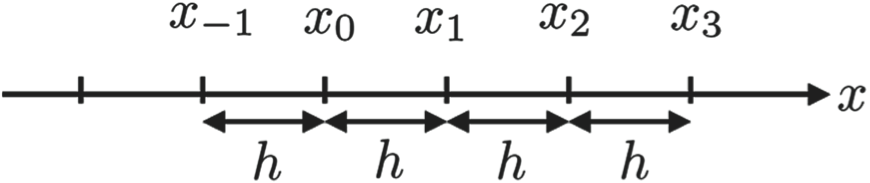
\includegraphics[width=10cm]{20.01.01-Numerical_grid}
%\caption{}
%\label{20.01.01-Numerical_gridfig1}
%\end{figure}
%
%\subsection*{Finite Difference Approximating Derivatives}
%The derivative $f′(x)$ of a function $f(x)$ at the point $x=a$ is defined as:
%\[f′(a)=\lim_{x\rightarrow a}\frac{f(x)-f(a)}{x-a}\]
%The derivative at $x=a$ is the slope at this point. In {\bf finite difference} approximations of this slope, we can use values of the function in the neighborhood of the point $x=a$ to achieve the goal. There are various finite difference formulas used in different applications, and three of these, where the derivative is calculated using the values of two points, are presented below.
%
%The {\bf forward difference} is to estimate the slope of the function at $x_j$ using the line that connects $(x_j,f(x_j))$ and $(x_{j+1},f(x_{j+1}))$:
%\[f′(x_j)=\frac{f(x_{j+1})-f(x_j)}{x_{j+1}-x_j}\]
%The {\bf backward difference} is to estimate the slope of the function at $x_j$ using the line that connects $(x_{j-1},f(x_{j-1}))$ and $(x_j,f(x_j))$:
%\[f′(x_j)=\frac{f(x_{j})-f(x_{j-1})}{x_{j}-x_{j-1}}\]
%The {\bf central difference} is to estimate the slope of the function at $x_j$ using the line that connects $(x_{j-1},f(x_{j-1}))$ and $(x_{j+1},f(x_{j+1}))$:
%\[f′(x_j)=\frac{f(x_{j+1})-f(x_{j-1})}{x_{j+1}-x_{j-1}}\]
%The following figure illustrates the three different type of formulas to estimate the slope.
%\begin{figure}[h]
%\centering
%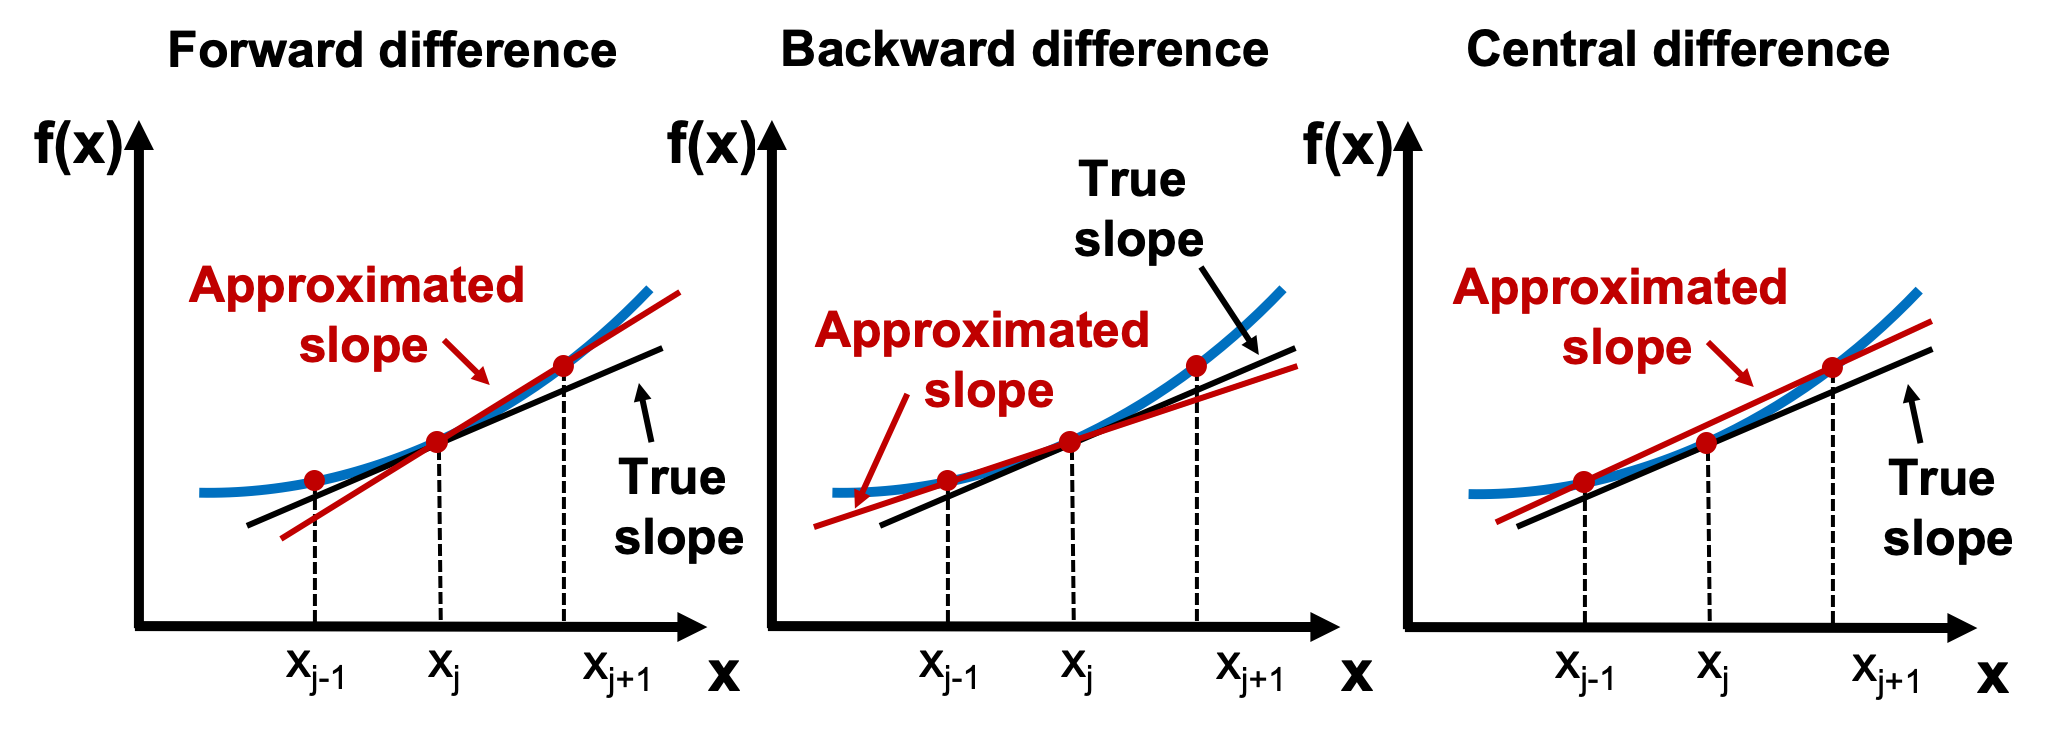
\includegraphics[width=14cm]{20.02.01-Finite-difference}
%\caption{}
%\label{20.02.01-Finite-differencefig2}
%\end{figure}
%
%\subsubsection*{Finite Difference Approximating Derivatives with Taylor Series}
%To derive an approximation for the derivative of $f$, we return to Taylor series. For an arbitrary function $f(x)$ the Taylor series of $f$ around $a=x_j$ is 
%\[f(x)=\frac{f(x_j)(x-x_j)^0}{0!}+\frac{f'(x_j)(x-x_j)^1}{1!}+\frac{f''(x_j)(x-x_j)^2}{2!}+\frac{f''(x_j)(x-x_j)^3}{3!}+\cdots\]
%If $x$ is on a grid of points with spacing $h$, we can compute the Taylor series at $x=x_{j+1}$ to get
%\[f(x_{j+1})=\frac{f(x_j)(x_{j+1}-x_j)^0}{0!}+\frac{f'(x_j)(x_{j+1}-x_j)^1}{1!}+\frac{f''(x_j)(x_{j+1}-x_j)^2}{2!}+\frac{f''(x_j)(x_{j+1}-x_j)^3}{3!}+\cdots\]
%Substituting $h=x_{j+1}−x_j$ and solving for $f'(x_j)$ gives the equation
%\[f'(x_j)=\frac{f(x_{j+1})-f(x_j)}{h}+\left(-\frac{f''(x_j)h}{2!}-\frac{f'''(x_j)h^2}{3!}-\cdots\right).\]
%The terms that are in parentheses, $-\frac{f''(x_j)h}{2!}-\frac{f'''(x_j)h^2}{3!}-\cdots,$ , are called higher order terms of $h$. The higher order terms can be rewritten as
%\[-\frac{f''(x_j)h}{2!}-\frac{f'''(x_j)h^2}{3!}-\cdots=h(\alpha+\epsilon(h),\]
%where $\alpha$ is some constant, and $\epsilon(h)$ is a function of $h$ that goes to zero as $h$ goes to $0$. We use the abbreviation $O(h)$ for $h(\alpha+\epsilon(h))$, and in general, we use the abbreviation $O(h^p)$  to denote $h^p(\alpha+\epsilon(h))$.
%
%Substituting $O(h)$ into the previous equations gives
%\[f'(x_j)=\frac{f(x_{j+1})-f(x_j)}{h}+O(h).\]
%This gives the {\bf forward difference} formula for approximating derivatives as
%\[f'(x_j)\approx\frac{f(x_{j+1})-f(x_j)}{h},\]
%and we say this formula is $O(h)$.
%
%Here, $O(h)$ describes the {\bf accuracy} of the forward difference formula for approximating derivatives. For an approximation that is $O(h^p)$, we say that $p$ is the order of the accuracy of the approximation. With few exceptions, higher order accuracy is better than lower order. To illustrate this point, assume $q<p$. Then as the spacing, $h>0$, goes to $0$, $h^p$ goes to $0$ faster than $h^q$. Therefore as $h$ goes to $0$, an approximation of a value that is $O(h^p)$ gets closer to the true value faster than one that is $O(h^q)$.
%
%By computing the Taylor series around $a=x_j$ at $x=x_{j-1}$ and again solving for $f'(x_j)$, we get the {\bf backward difference} formula
%\[f'(x_j)\approx\frac{f(x_j)-f(x_{j-1})}{h},\]
%which is also $O(h)$.
%
%Intuitively, the forward and backward difference formulas for the derivative at $x_j$ are just the slopes between the point at $x_j$ and the points $x_{j+1}$ and $x_{j-1}$, respectively.
%
%We can construct an improved approximation of the derivative by clever manipulation of Taylor series terms taken at different points. To illustrate, we can compute the Taylor series around $a=x_j$ at both $x_{j+1}$ and $x_{j-1}$. Written out, these equations are
%\[f(x_{j+1})=f(x_j)+f'(x_j)h+\frac12f''(x_j)h^2+\frac16f'''(x_j)h^3+\cdots\]
%and
%\[f(x_{j-1})=f(x_j)-f'(x_j)h+\frac12f''(x_j)h^2-\frac16f'''(x_j)h^3+\cdots\]
%Subtracting the formulas above gives
%\[f(x_{j+1})-f(x{j-1})=2f'(x_j)+\frac23f'''(x_j)h^3+\cdots,\]
%which when solved for $f'(x_j)$ gives the central difference formula
%\[f'(x_j)\approx\frac{f(x_{j+1})-f(x_{j-1})}{2h}.\]
%Because of how we subtracted the two equations, the $h$ terms canceled out; therefore, the central difference formula is $O(h^2)$, even though it requires the same amount of computational effort as the forward and backward difference formulas! Thus the central difference formula gets an extra order of accuracy for free. In general, formulas that utilize symmetric points around $x_j$, for example $x_{j-1}$ and $x_{j+1}$, have better accuracy than asymmetric ones, such as the forward and background difference formulas.
%
%The following figure shows the forward difference (line joining$ (x_j,y_j)$ and $(x_{j+1},y_{j+1})$), backward difference (line joining $(x_j,y_j)$ and $(x_{j-1},y_{j-1})$), and central difference (line joining $(x_{j-1},y_{j-1})$ and $(x_{j+1},y_{j+1})$) approximation of the derivative of a function $f$. As can be seen, the difference in the value of the slope can be significantly different based on the size of the step $h$ and the nature of the function.
%\begin{figure}[h]
%\centering
%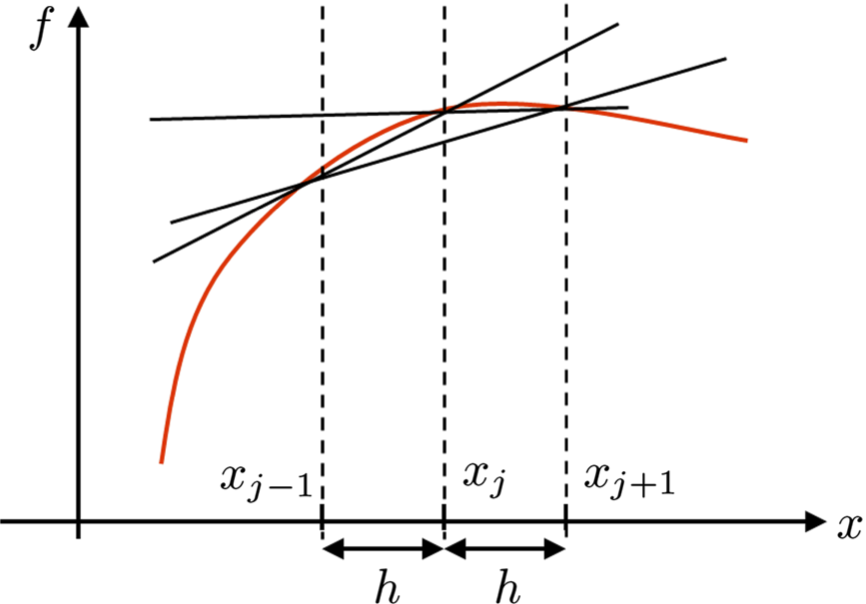
\includegraphics[width=10cm]{20.02.01-Forward_difference}
%\caption{}
%\label{20.02.01-Forward_differencefig3}
%\end{figure}
%
%\begin{example}
%Take the Taylor series of $f$ around $a=x_j$ and compute the series at $x=x_{j-2}$, $x_{j-1}$, $x_{j+1}$, $x_{j+2}$. Show that the resulting equations can be combined to form an approximation for $f'(x_j)$ that is $O(h^4)$.
%\end{example}
%
%\begin{mysolution}
%First, compute the Taylor series at the specified points.
%\[\begin{split}
%f(x_{j-2})&=f(x_j)-2hf'(x_j)+\frac{4h^2f''(x_j)}{2}-\frac{8h^3f'''(x_j)}{6}+\frac{16h^4f''''(x_j)}{24}-\frac{32h^5f'''''(x_j)}{120}+\cdots\\[2mm]
%f(x_{j-1})&=f(x_j)-hf'(x_j)+\frac{h^2f''(x_j)}{2}-\frac{h^3f'''(x_j)}{6}+\frac{h^4f''''(x_j)}{24}-\frac{h^5f'''''(x_j)}{120}+\cdots\\[2mm]
%f(x_{j+1})&=f(x_j)+hf'(x_j)+\frac{h^2f''(x_j)}{2}+\frac{h^3f'''(x_j)}{6}+\frac{h^4f''''(x_j)}{24}+\frac{32h^5f'''''(x_j)}{120}+\cdots\\[2mm]
%f(x_{j+2})&=f(x_j)+2hf'(x_j)+\frac{4h^2f''(x_j)}{2}+\frac{8h^3f'''(x_j)}{6}+\frac{16h^4f''''(x_j)}{24}+\frac{32h^5f'''''(x_j)}{120}+\cdots
%\end{split}\]
%To get the $h^2$, $h^3$, and $h^4$ terms to cancel out, we can compute
%\[f(x_{j-2})-8f(x_{j-1})+8f(x_{j-1})-f(x_{j+2})=12hf'(x_j)-\frac{48h^5f'''''(x_j)}{120}\]
%which can be rearranged to
%\[f'(x_j)=\frac{f(x_{j-2})-8f(x_{j-1})+8f(x_{j-1})-f(x_{j+2})}{12h}+O(h^4).\]
%This formula is a better approximation for the derivative at $x_j$ than the central difference formula, but requires twice as many calculations.
%\end{mysolution}


Python uses the following command to compute finite differences directly: for a vector $f$, the command $d=np.diff(f)$ produces an array $d$ in which the entries are the differences of the adjacent elements in the initial array $f$. In other words $d(i)=f(i+1)-f(i)$.



When using the command $np.diff$, the size of the output is one less than the size of the input since it needs two arguments to produce a difference.


\begin{example}
Consider the function f(x)=cos(x)
. We know the derivative of cos(x)
 is −sin(x)
. Although in practice we may not know the underlying function we are finding the derivative for, we use the simple example to illustrate the aforementioned numerical differentiation methods and their accuracy. The following code computes the derivatives numerically.
\end{example}

\begin{boxB}
import numpy as np\\
import matplotlib.pyplot as plt\\
plt.style.use('seaborn-poster')\\
%matplotlib inline\\
\end{boxB}

\begin{boxB}
\# step size\\
$h = 0.1$\\
\# define grid\\
$x = np$.arange(0, 2*np.pi, h) \\
\# compute function\\
$y = np.cos(x)$ \\
\\
\# compute vector of forward differences\\
forward\_diff = np.diff(y)/h \\
\# compute corresponding grid\\
$x_diff = x[:-1:]$ \\
\# compute exact solution\\
exact\_solution = -np.sin(x\_diff) \\
\\
\# Plot solution\\
plt.figure(figsize = (12, 8))\\
plt.plot(x\_diff, forward\_diff, '--', \textbackslash \\
         \hspace*{2cm}label = 'Finite difference approximation')\\
plt.plot(x\_diff, exact\_solution, \textbackslash \\
         \hspace*{2cm}label = 'Exact solution')\\
plt.legend()\\
plt.show()\\
\\
\# Compute max error between \\
\# numerical derivative and exact solution\\
max\_error = max(abs(exact\_solution - forward\_diff))\\
print(max\_error)\\
\end{boxB}
\newpage
\begin{figure}[h]
\centering
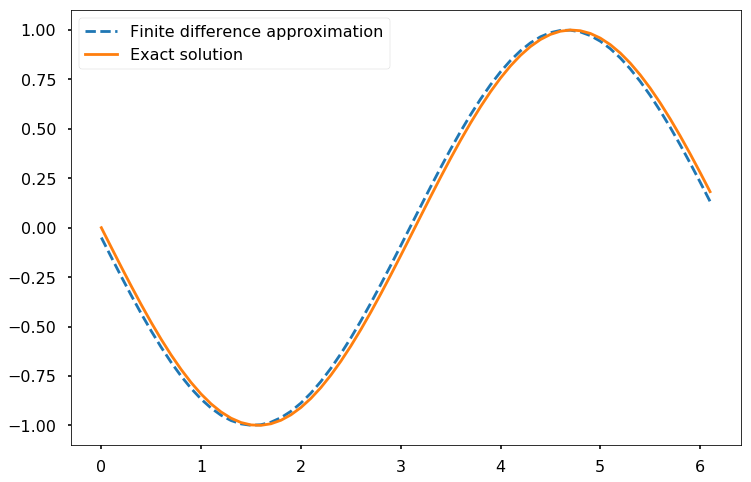
\includegraphics[width=12cm]{chapter20.02-Finite-Difference-Approximating-Derivatives_5_0}
\caption{}
\label{}
\end{figure}

0.049984407218554114

As the above figure shows, there is a small offset between the two curves, which results from the numerical error in the evaluation of the numerical derivatives. The maximal error between the two numerical results is of the order $0.05$ and expected to decrease with the size of the step.

As illustrated in the previous example, the finite difference scheme contains a numerical error due to the approximation of the derivative. This difference decreases with the size of the discretization step, which is illustrated in the following example.

\begin{example}
The following code computes the numerical derivative of $f(x)=\cos(x)$ using the forward difference formula for decreasing step sizes, $h$. It then plots the maximum error between the approximated derivative and the true derivative versus $h$ as shown in the generated figure.

\begin{boxB}
\# define step size\\
$h = 1$\\
\# define number of iterations to perform\\
iterations = 20 \\
\# list to store our step sizes\\
step\_size = [] \\
\# list to store max error for each step size\\
max\_error = [] \\
\\
for i in range(iterations):\\
    \hspace*{0.5cm}\# halve the step size\\
    \hspace*{0.5cm}h /= 2 \\
    \hspace*{0.5cm}\# store this step size\\
    \hspace*{0.5cm}step\_size.append(h) \\
    \hspace*{0.5cm}\# compute new grid\\
    \hspace*{0.5cm}x = np.arange(0, 2 * np.pi, h) \\
    \hspace*{0.5cm}\# compute function value at grid\\
    \hspace*{0.5cm}y = np.cos(x) \\
    \hspace*{0.5cm}\# compute vector of forward differences\\
    \hspace*{0.5cm}forward\_diff = np.diff(y)/h \\
    \hspace*{0.5cm}\# compute corresponding grid\\
    \hspace*{0.5cm}x\_diff = x[:-1] \\
    \hspace*{0.5cm}\# compute exact solution\\
    \hspace*{0.5cm}exact\_solution = -np.sin(x\_diff) \\
\\    
    \hspace*{0.5cm}\# Compute max error between \\
    \hspace*{0.5cm}\# numerical derivative and exact solution\\
    \hspace*{0.5cm}max\_error.append(\textbackslash \\
            \hspace*{2cm}max(abs(exact\_solution - forward\_diff)))\\
\\
\# produce log-log plot of max error versus step size\\
plt.figure(figsize = (12, 8))\\
plt.loglog(step\_size, max\_error, 'v')\\
plt.show()\\
\end{boxB}

\begin{center}
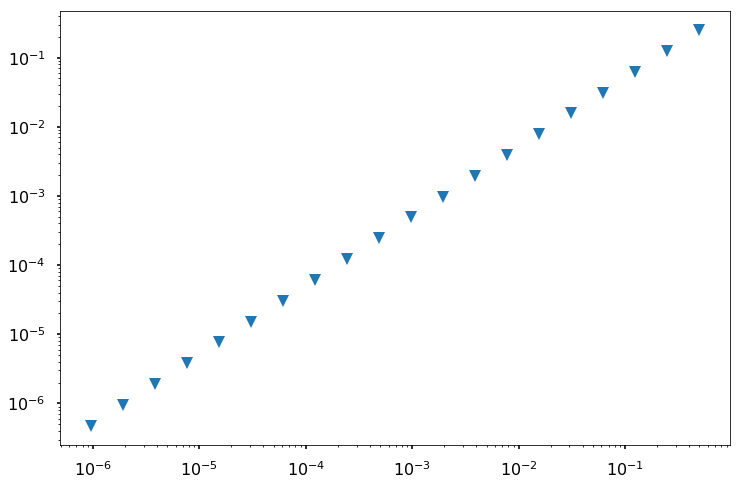
\includegraphics[width=13cm]{chapter20.02-Finite-Difference-Approximating-Derivatives_7_0}
%\caption{}
%\label{}
\end{center}
The slope of the line in log-log space is $1$; therefore, the error is proportional to $h^1$, which means that, as expected, the forward difference formula is $O(h)$.
\end{example}


%\begin{myexercise}\label{Comprehensionquiz2}
%%\begin{enumerate}[label=\arabic*.]
%%\item 
%%
%%\end{enumerate}
%\end{myexercise}

\section{Numerical Differentiation with Noise}
\videolesson
\begin{selfvideo}[2]
%LESSON 3: 
This video presents a discussion on numerical differentiation with noise. Follow the discussion and then solve the problems in the subsequent quiz.
\end{selfvideo}

As stated earlier, sometimes $f$ is given as a vector where $f$ is the corresponding function value for independent data values in another vector $x$, which is gridded. Sometimes data can be contaminated with {\bf noise}, meaning its value is off by a small amount from what it would be if it were computed from a pure mathematical function. This can often occur in engineering due to inaccuracies in measurement devices or the data itself can be slightly modified by perturbations outside the system of interest. For example, you may be trying to listen to your friend talk in a crowded room. The signal $f$ might be the intensity and tonal values in your friend’s speech. However, because the room is crowded, noise from other conversations are heard along with your friend’s speech, and he becomes difficult to understand.

To illustrate this point, we numerically compute the derivative of a simple cosine wave corrupted by a small sin wave. Consider the following two functions:
\[f(x)=\cos(x)\]
and
\[f_{\epsilon,\omega}(x)=\cos(x)+\epsilon\sin(\omega x)\]
where $0<\epsilon\ll1$ is a very small number and $\omega$ is a large number. When $\epsilon$ is small, it is clear that $f\simeq f_{\epsilon,\omega}$. To illustrate this point, we plot $f_{\epsilon,\omega}(x)$ for $\epsilon=0.01$ and $\omega=100$, and we can see it is very close to $f(x)$, as shown in the following figure.

\begin{boxB}
import numpy as np\\
import matplotlib.pyplot as plt\\
plt.style.use('seaborn-poster')\\
\%matplotlib inline
\end{boxB}

\begin{boxB}
x = np.arange(0, 2*np.pi, 0.01) \\
\# {\it compute function}\\
omega = 100\\
epsilon = 0.01\\
\\
y = np.cos(x) \\
y\_noise = y + epsilon*np.sin(omega*x)\\
\\
\# {\it Plot solution}\\
plt.figure(figsize = (12, 8))\\
plt.plot(x, y\_noise, 'r$^-$', \textbackslash \\
         \hspace*{1.5cm}label = 'cos(x) + noise')\\
plt.plot(x, y, 'b-', \textbackslash \\
         \hspace*{1.5cm}label = 'cos(x)')\\
\\
plt.xlabel('x')\\
plt.ylabel('y')\\
\\
plt.legend()\\
plt.show()\\
\end{boxB}

\begin{figure}[h]
\centering
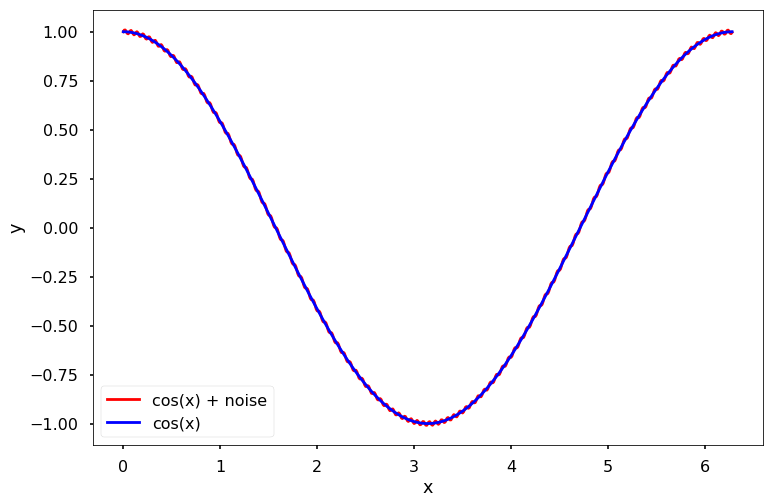
\includegraphics[width=13cm]{chapter20.04-Numerical-Differentiation-with-Noise_5_0}
\caption{}
\label{}
\end{figure}


The derivatives of our two test functions are
\[f'(x)=-\sin x\quad\mbox{ and }\quad f'_{\epsilon,\omega}(x)=-\sin x+\epsilon\omega\cos(\omega x).\]

Since $\epsilon\omega$ may not be small when $\omega$ is large, the contribution of the noise to the derivative may not be small. As a result, the derivative (analytic and numerical) may not be usable. For instance, the following figure shows $f'(x)$ and $f'_{\epsilon,\omega}(x)$ for $\epsilon=0.01$ and $\omega=100$.

\begin{boxB}
x = np.arange(0, 2*np.pi, 0.01) \\
\# compute function\\
y = -np.sin(x) \\
y\_noise = y + epsilon*omega*np.cos(omega*x)\\
\\
\# Plot solution\\
plt.figure(figsize = (12, 8))\\
plt.plot(x, y\_noise, 'r$^-$', \textbackslash \\
        \hspace*{1.5cm} label = 'Derivative cos(x) + noise')\\
plt.plot(x, y, 'b-', \textbackslash \\
        \hspace*{1.5cm} label = 'Derivative of cos(x)')\\
\\
plt.xlabel('x')\\
plt.ylabel('y')\\
\\
plt.legend()\\
plt.show()
\end{boxB}

\begin{figure}[h]
\centering
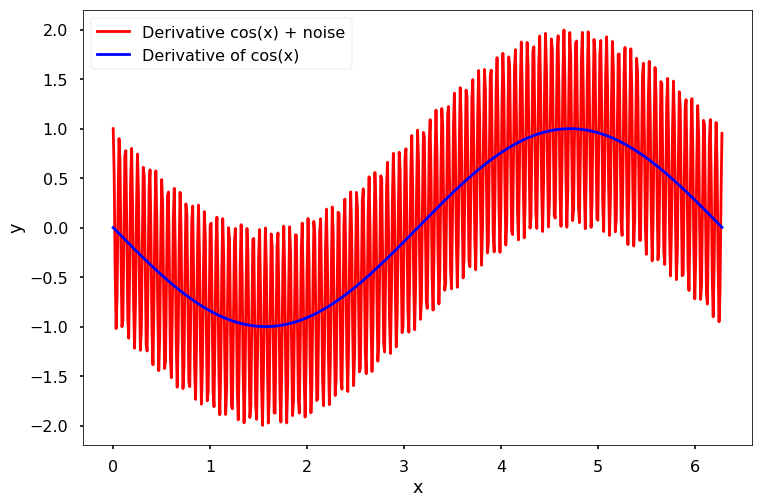
\includegraphics[width=12cm]{chapter20.04-Numerical-Differentiation-with-Noise_7_0}
\caption{}
\label{}
\end{figure}

%\begin{youtube}
%This video presents a discussion on numerical differentiation with noise. Follow the discussion and then solve the problems in the subsequent quiz.
%\end{youtube}


%\begin{myexercise}\label{Comprehensionquiz2}
%%\begin{enumerate}[label=\arabic*.]
%%\item 
%%
%%\end{enumerate}
%\end{myexercise}



\section{Riemann's Integral, Trapezoidal Rule and Simpson's Rule in Python}
\activities
Read stated reference on Riemann's integral, trapezoidal rule and Simpson's rule in python in the given web pages and then attempt the subsequent quiz.
\begin{activity}[\cg Reading]
\begin{enumerate}
\item Kong, Q., Siauw, T., Bayen, A., (2020). Python Programming and Numerical Methods. First Edition, Academic Press,  ISBN-13 ‏ : ‎ 978-0128195499 \\
\mylink{https://pythonnumericalmethods.studentorg.berkeley.edu/notebooks/chapter21.02-Riemanns-Integral.html}\\
\mylink{https://pythonnumericalmethods.studentorg.berkeley.edu/notebooks/chapter21.03-Trapezoid-Rule.html}
\mylink{https://pythonnumericalmethods.studentorg.berkeley.edu/notebooks/chapter21.04-Simpsons-Rule.html}
\end{enumerate}
\end{activity}
%\begin{myexercise}\label{Comprehensionquiz2}
%\begin{enumerate}[label=\arabic*.]
%\item 
%
%\end{enumerate}
%\end{myexercise}



%\begin{example}
%
%\end{example}
%
%\begin{mysolution}
%
%\end{mysolution}
%
%
%
%\begin{example}%\label{2ndorderpatderivative}
%
%\end{example}
%
%\begin{mysolution}
%
%\end{mysolution}



%\begin{myexercise}\label{Comprehensionquiz2}
%
%\end{myexercise}


\section{Computing Integrals in Python}
%\videolesson
%\begin{selfvideo}[2]
%%LESSON 3: 
%This video presents a discussion on computing integral in python. Follow the discussion and then solve the problems in the subsequent quiz.
%\end{selfvideo}
\begin{youtube}
This video presents a discussion on computing integral in python. Follow the discussion and then solve the problems in the subsequent quiz.
\end{youtube}
\mylink{https://www.youtube.com/watch?v=2I44Y9hfQ4Q}
%\begin{boxB}Question: \end{boxB}
%\begin{myexercise}\label{Comprehensionquiz2}
%%\begin{enumerate}[label=\arabic*.]
%%\item 
%%
%%\end{enumerate}
%\end{myexercise}


%\discussion


\begin{posttest}[\textcolor{red}{End of Module 9 Quiz}]
\item Consider the integral $\int_0^1x^2\,dx$. Using the trapezoidal rule write a python code for the definite integral and hence evaluate the integral
\item Find the work produced (𝑾) in a piston cylinder device using SciPy Module {\bf scipy.integrate}
\item Evaluate $\int_{-1}^1(𝑥^3 +2𝑥^2-𝑥+3)\,dx$ by writing a python code for both the indefinite and definite integrals.
\begin{mysolution}
\begin{enumerate}[label=\arabic*.]
\item ~\\
\begin{boxB}
import numpy as np\\
% import matplotlib.pyplot as plt\\
 a = 0; b = 1\\
 N = 10\\
\\
 x = np.linspace(a,b,N+1)\\
\\
 y = x**2;\\
\\
 y\_right = y[1:]\\
 y\_left = y[:-1]\\
\\
\# Trapezoid Rule\\
 dx = (b - a)/N\\
 A = (dx/2) * np.sum(y\_right + y\_left)\\
 print("A =", A)\\
%\\
%plt.plot(x,y)
% plt.xlim([0,1]); plt.ylim([0,1]);
\end{boxB}


\begin{boxB}
 import matplotlib.pyplot as plt\\
 import numpy as np\\
 xstart = 0\\
 xstop = 1.1\\
 increment = 0.1\\
\\
 x = np.arange(xstart, xstop, increment)\\
 y = x**2\\
\\
 plt.plot(x, y)\\
 plt.xlabel('x')\\
 plt.ylabel('y')\\
 plt.axis([0, 1, 0, 1])\\
 plt.fill\_between(x,y)\\
 plt.show()
\end{boxB}
\[f(x)=x^2\quad \int_0^1x^2\,dx=\frac13\approx0.3333\]


\begin{center}
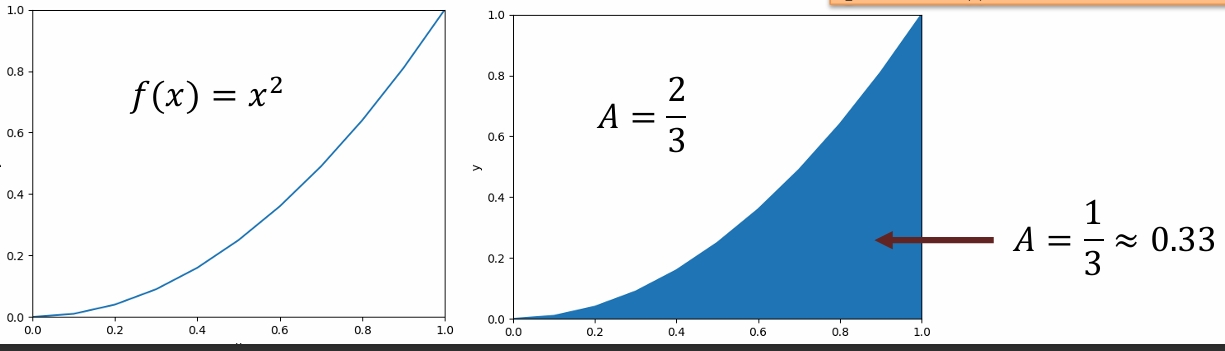
\includegraphics[width=15cm]{EndofMod9Q1sol}
\end{center}
Results from the Python code: $A = 0.3350000000000001$

\item ~\\
\begin{boxB}
from scipy import integrate\\
\\
 V1 = 1 \\
V2 = 5 \\
\\
n = 1\\
 R = 8.314\\
 T = 300\\
\\
 def work\_eq(V, n, R, T):\\
\hspace*{1cm} W = (n*R*T)/V  \\
\hspace*{1cm}return W\\
\\
 W, e = integrate.quad(work\_eq, V1, V2, args=(n, R, T,))\\
\\
 print("W =", W)
\end{boxB}

$W = 4014.2600411931353$

\item~\\
\begin{boxB}
import numpy.polynomial.polynomial as poly\\
\\
 p = [3, -1, 2, 1]\\
\\
 \# Find Indefinite integral\\
 I = poly.polyint(p)\\
 print("I =", I)\\

 \# Find Definite integral\\
 a = -1\\
 b = 1\\
\\
 A = poly.polyval(b, I) -poly.polyval(a, I)\\
 print("A =", A)
\end{boxB}

The Python solution: 
\[ I = [ 0.  3.  -0.5  0.66666667  0.25 ],\quad A = 7.333333333333333\]
\end{enumerate}
\end{mysolution}

\end{posttest}

%share your understanding of properties of functions and their applications to solving rates of change problems in physical phenomenon 


%\end{actsoln}

\takehome

\comy{You are now at the last part of this module. Your  task is to do a self-reflection on your learning experience.}



\references
\begin{refenumerate}
\item Kong, Q., Siauw, T., Bayen, A., (2020). Python Programming and Numerical Methods. First Edition, Academic Press,  ISBN-13 ‏ : ‎ 978-0128195499 \\
\mylink{https://pythonnumericalmethods.studentorg.berkeley.edu/notebooks/Index.html}
%chapter 1 pg 7-36 functions\\
%chapter 1 pg 51-83 limits and continuity\\
%chapter 1 pg 45-50 rates of change\\
%chapter 2 pg 108-120 the derivative\\
%\item Mendelson, E. (2022). Schaum's Outline of Calculus. McGraw-Hill Education.
%chapter 6 51-55 functions
%chapter 7 59-65 limits
%chapter 8 69-74 continuity
%chapter 9 77-81 derivative
%\item Calculus \mylink{https://math.libretexts.org/Bookshelves/Calculus}
%\item Chris McMullen, 2021, Essential Calculus Skills Practice Workbook with Full Solutions, Zishka Publishing, ISBN 978-1-941691-24-3
%\item R. Adams and C. Essex, 2021, Calculus: A complete Course, Addison Wesley, ISBN 13: 978-0135732588
%\item P. Abbott and H. Neill, 2018, Calculus: A Complete Introduction: The Easy Way to Learn Calculus (Teach Yourself), ISBN 13: 978-1473678446
\end{refenumerate}





%\wrapup
%To wrap-up, answer the following questions:
%
%\begin{enumerate}
%\item 
%%when do we say that a limit of a function exists?
%%\item how do we remove discontinuity in functions?
%%\item what is the relationship between the gradient of the tangent line and the derivative?
%\end{enumerate}
















%\newpage

%\facilitation


%
\begin{center}
    {\Large \textbf{FUNCTIONS OF SEVERAL VARIABLES}}\\[2mm]
(DEFINITION, DOMAIN, RANGE, GRAPHS AND LEVEL CURVES) \\[4mm]

\mycenterbox{5 minute review}%\\[4mm]
Recap the definition of a function of several variables, and the meaning of domain, range, graph and level curves of functions of several variables.
\end{center}
\mycenterbox{Warm-up.}%\\[4mm]
\problemAnswer{
Match the function with its graph (labeled I–VI).Give reasons for your choices
\begin{multicols}{3}
\begin{enumerate}[label=(\alph*)]
\item $f(x,y)=|x|+|y|$\\[4mm]
\item $f(x,y)=|xy|$
\item $f(x,y)=\frac{1}{1+x^2+y^2}$\\2mm]
\item $f(x,y)=(x^2-y^2)^2$
\item $f(x,y)=(x-y)^2$\\[4mm]
\item $f(x,y)=\sin(|x|+|y|)$
\end{enumerate}
\end{multicols}

\begin{center}
%\centering
\includegraphics[width=10cm]{MCTutorial1Q1.JPEG}
\end{center}
%\tcbox[tcbox raise base]{Warm-up}
 
%\begin{flushright}
%\begin{tikzpicture}
%    % A body
%
%
%    % Non-rectangle shapes must be drawn as polygone
%    \begin{scope}[shift={(3,0)}]
%        \draw  (0,0.5) -- (0,4) -- (.5,4) -- (.5,4.5) -- (1.,4.5) -- (4.,4.5) --(4.,4)-- (4.5,4) --(4.5,0.5) --(4.0,0.5)--(4.0,0.0)-- (.5,0) --(0.5,0.5) -- cycle;
%        % Draw symmetry lines
%        \draw [symmetry] (.5, 0.5) -- (.5,4.0);
%        \draw [symmetry] (4, 0.5) -- (4,4.0);
%        \draw [symmetry] (.5,4.0) -- (4,4.0);
%         \draw [symmetry] (.5, 0.5) -- (4, 0.5);
%        % Dimensions
%        \draw (4.5,0) -- ++(0.5,0) coordinate (D1) -- +(5pt,0);
%        \draw (4.5,4.5) -- ++(0.5,0) coordinate (D2) -- +(5pt,0);
%        \draw [dimen] (D1) -- (D2) node {6cm};
%       
%        
%        \draw (0.0,5) -- ++(0,0.5) coordinate (D1) -- +(0,+5pt);
%        \draw (0.5,5) -- ++(0,0.5) coordinate (D2) -- +(0,+5pt);
%        \draw [dimen,-] (D1) -- (D2) node [above=5pt] {$x$ cm};
%        \draw [dimen,<-] (D1) -- ++(-5pt,0);
%        \draw [dimen,<-] (D2) -- ++(+5pt,0);
%    \end{scope}
%\end{tikzpicture}
%\end{flushright}

}


\mycenterbox{Problems.}%

%\begin{center}
%\tcbox[tcbox raise base]{ Problems. Choose from the below}
%\end{center}
\problem{Exploring functions}%
\begin{enumerate}[(a)]
\item Are the following functions even, odd, or neither? What can you say
about their range?
\begin{multicols}{4}
 \begin{enumerate}[(i)]
\item $\displaystyle \frac{3x}{x^2+2}$
\item $\displaystyle \cos x+3$
\item $\displaystyle \frac{2x^3}{\cos x+3}$
\item $\displaystyle \frac{3x^4+2x^2}{\sin x+4}$
\end{enumerate}
\end{multicols}
\item Consider the functions $\sin^n x$ and $\cos^n x$, where $n$ is a positive integer.
Which are odd, which are even, and what are their periodicities?
\item What is the periodicity of $f(x) = 2 \cos x+\sin 2x$? Is it even/odd/neither?

\end{enumerate}

\problem{Cubic functions} 
Show that $x-1$ is a factor of the cubic function%
$$P(x)=x^3-2x^2-5x+6,$$
and  find the quadratic factor $Q(x)$ such that $P(x) = (x -1)Q(x)$. Factorise
$Q(x)$ and hence sketch $P(x).$

%\newpage
\problem{Sigmoid functions*.}%
For positive integers $n$, consider the family of functions
$$\displaystyle f_n= \frac{x^n}{2^n+x^n}.$$
\begin{enumerate}[(a)]
\item What are appropriate domains and ranges for $f_n(x)$? Do they depend on $n$?

\item Is $f_n(x)$ even, odd, or neither? Does this depend on $n$?

\item Show that for $x\geq 0$, $f_n(x)$ are strictly increasing functions and that
$0\leq f_n(x) < 1.$
\item What is the value of $f_n(2)$? Does it depend on $n$?

\item By considering the values of $f_n(1.9)$ and $f_n(2.1)$ for $n = 2, 4, 8, 16, 32$ and
$64$, show that the graph of $f_n(x)$ for $x\ge 0$ is an increasing sigmoid (that
is, $S$-shaped) function that approaches a step function as $n\rightarrow \infty$.
\end{enumerate}

\mycenterbox{Selected answers and hints}%

For the warm-up, $V(x)=4x(3-x)^2$. Writing $x=1+\epsilon$, we get
$$V = 4(1 +\epsilon)(3- (1+\epsilon))^2=4(4-\epsilon^2(3-\epsilon)).$$
If $-1<\epsilon<2$ then $\epsilon^2 (3-\epsilon)\ge 0$, with equality when $\epsilon=0$. Thus the maximum
value of $V$ occurs when $\epsilon= 0$, i.e. $x = 1\rm{cm}$.

\begin{enumerate}
\item 
\begin{enumerate}[(i)]
\item Odd. The range is the interval  $[-\frac{3}{4}\sqrt{2},\; \frac{3}{4}\sqrt{2}]$
\item Even. The range is the interval $[2, 4]$.
\item Odd. The range is all of $\mathbb R$.
\item Neither. (For example, writing $\displaystyle \frac{5}{\sin x+4}$ we have $\displaystyle f(1)= \frac{5}{\sin (1)+4} \equiv 1.032 (3\rm{dp})$ which is neither $f(1)$ nor $-f(1)$.)\\[4mm]
The range is the nonnegative reals $[0,\infty)$

\end{enumerate}
\end{enumerate}











%
%\newtheorem{definition}[subsection]{Definition}
%\newtheorem{example}[subsection]{Example}
\newtheorem{cor}[subsection]{Corollary}
\newtheorem{pro}[subsection]{Proposition}
\newtheorem{theo}[subsection]{Theorem}
\newtheorem{lem}[subsection]{Lemma}
%\newtheorem{rem}[subsection]{Remark}

\definecolor{main}{HTML}{5989cf}    % setting main color to be used
\definecolor{sub}{HTML}{cde4ff}     % setting sub color to be used

\tcbset{
    sharp corners,
    colback = white,
    before skip = 0.2cm,    % add extra space before the box
    after skip = 0.5cm      % add extra space after the box
}                           % setting global options for tcolorbox

% You can copy any following box you like to your code.
\newtcolorbox{boxA}{
    fontupper = \bf,
    boxrule = 1.5pt,
    colframe = black % frame color
}

\newtcolorbox{boxB}{
    fontupper = \bf\color{main}, % font color
    boxrule = 1.5pt,
    colframe = main,
    rounded corners,
    arc = 5pt   % corners roundness
}
\newtcolorbox{boxC}{
    colback = sub, % background color
    boxrule = 0pt  % no borders
}

\newtcolorbox{boxD}{
    colback = sub, 
    colframe = main, 
    boxrule = 0pt, 
    toprule = 3pt, % top rule weight
    bottomrule = 3pt % bottom rule weight
}

\hypersetup{
    colorlinks=true,
    linkcolor=blue,
    filecolor=magenta,      
    urlcolor=cyan,
    pdftitle={Overleaf Example},
    pdfpagemode=FullScreen,
    }

\urlstyle{same}


\coursetitle{\mtthreeiii}{MT303}
\developers{Wyclife Rao}
\reviewers{Dr Irene Sitawa}
\modulenumber{10}
\modulename{Numerical Methods for Ordinary Differential Equations Using Python}

% courses
\thispagestyle{empty}
\begin{tikzpicture}[overlay,remember picture,font=\sffamily\bfseries]
 \draw[ultra thick,c4,name path=big arc] ([xshift=-2mm]current page.north) arc(150:285:11) coordinate[pos=0.225] (x0);
 \begin{scope}
  \clip ([xshift=-2mm]current page.north) arc(150:285:11) --(current page.north east);
  \fill[c4!50,opacity=0.25] ([xshift=4.55cm]x0) circle (4.55);
  \fill[c4!50,opacity=0.25] ([xshift=3.4cm]x0) circle (3.4);
  \fill[c4!50,opacity=0.25] ([xshift=2.25cm]x0) circle (2.25);
  \draw[ultra thick,c4!50] (x0) arc(-90:30:6.5);
  \draw[ultra thick,c4] (x0) arc(90:-30:8.75);
  \draw[ultra thick,c4!50,name path=arc1] (x0) arc(90:-90:4.675);
  \draw[ultra thick,c4!50] (x0) arc(90:-90:2.875);
  \path[name intersections={of=big arc and arc1,by=x1}];
  \draw[ultra thick,c4,name path=arc2] (x1) arc(135:-20:4.75);
  \draw[ultra thick,c4!50] (x1) arc(135:-20:8.75);
  \path[name intersections={of=big arc and arc2,by={aux,x2}}];
  \draw[ultra thick,c4!50] (x2) arc(180:50:2.25);
 \end{scope} 
 \path[decoration={text along path,text color=c4,
                 raise = -2.8ex,
                 text  along path,
                 text = {},%|\sffamily\bfseries|02/18/2019
                 text align = center,
             },
             decorate
         ] ([xshift=-2mm]current page.north) arc(150:245:11);
 %
 \newcommand\add{4cm}
 \begin{scope}%[shift={(5,0)}]
  \path[clip,postaction={fill=c3}]
  ([xshift=2cm+\add,yshift=-8cm]current page.center) rectangle ++ (4.6,7.7);
  \draw[c5,ultra thick,fill=c2] ([xshift=0.5cm+\add,yshift=-8cm]current page.center)
   ([xshift=0.5cm+\add,yshift=-8cm]current page.center)  arc(180:60:2)
    |- ++ (-3,6) --cycle;
  \draw[ultra thick,c5] ([xshift=-1.5cm+\add,yshift=-8cm]current page.center) 
  arc(180:0:2);
  \draw[ultra thick,c5] ([xshift=0.5cm+\add,yshift=-8cm]current page.center) 
  arc(180:0:2);
  \draw[ultra thick,c5] ([xshift=2.5cm+\add,yshift=-8cm]current page.center) 
  arc(180:0:2);
  \draw[ultra thick,c5] ([xshift=4.5cm+\add,yshift=-8cm]current page.center) 
  arc(180:0:2);
  \fill[white] ([xshift=2.5cm+\add,yshift=-8cm]current page.center) +(60:2) circle(1.5mm)
  node[above
  right=0mm,text=c5!80!black]{$\rho:=\dfrac{1+\sqrt{-3}}{2}$};
 \end{scope}
 %
 \fill[c1] ([xshift=2cm+\add,yshift=-8cm]current page.center) rectangle ++ (-30.7,7.7);
 \node[text=white,anchor=west,scale=2.3,inner sep=0pt] at
 ([xshift=-10cm,yshift=-1.8cm]current page.center) {\color{ulabgold} LEARNING};
 \node[text=white,anchor=west,scale=5,inner sep=0pt] at
 ([xshift=-10cm,yshift=-3.25cm]current page.center) {MODULE \dpmdnumber};
 \node[text=white,anchor=west,scale=2.5,inner sep=0pt,text width=.4\textwidth] at
 ([xshift=-10cm,yshift=-6cm]current page.center) {\dpmdname};
 \node[text=white,anchor=east,scale=2,inner sep=0pt] at
 ([xshift=5.7cm,yshift=-7.5cm]current page.center) {\color{ulabgold}The Open University of Kenya};
 %
% \draw[gray,line width=5mm] 
% ([xshift=2mm,yshift=-1mm]current page.south west) rectangle ([xshift=-2mm,yshift=1mm]current
% page.north east);
\end{tikzpicture}

%\newpage
\pagenumbering{roman}
\thispagestyle{empty}%firstpage


\begin{center}
\vspace*{2cm}
{\Huge\bf BACHELOR OF TECHNOLOGY EDUCATION}\\[3cm]  


%{\fontsize{80}{40}\selectfont \dpcoursecode}\\[2cm]
%
%{\fontsize{30}{40} \selectfont \dpcoursename}\\[2cm]

%\rule{\textwidth}{1pt}
%\vspace{2cm}

%{\fontsize{40}{40}\selectfont \bf Module~\dpmdnumber}\\[2cm]
%
%{\fontsize{30}{40}\selectfont \bf \dpmdname}\\

\vfill
\begin{flushright}
\begin{minipage}{.6\textwidth}
\begin{tcolorbox}%[text ]
\begin{tabular}{ll}%\hline
\subtitle{Developed by:}&\displaydevelopers\\
&\\
\subtitle{Reviewed by:}&\makecell[l]{\displayreviewers}\\
\end{tabular}
\end{tcolorbox}
\end{minipage}\hspace*{-3.5cm}
\end{flushright}
\vspace*{-2.5cm}
\end{center}

\newpage
\thispagestyle{empty}
\null
\vfill
{\renewcommand\arraystretch{1.5}
\begin{tabular}{|l|l|}\hline
\subtitle{Programme Title} & Bachelor of Technology Education \\\hline
\subtitle{Course Title} & \fullcoursename\\\hline
\subtitle{Learning Module number} & Module \dpmdnumber\\\hline
\subtitle{Learning module title} & \dpmdname \\\hline
\subtitle{Module Developer} & \displaydevelopers\\\hline
\subtitle{Reviewed by} & \displayreviewers\\\hline
%\subtitle{Vision} & \vision\\\hline
%\subtitle{Audience description} & \\\hline
\end{tabular}}
\clearpage

%\section{COURSE LEARNING GUIDE}


\subsection*{Preparing for Online and Distance Learning}

This course offers you the opportunity to enter an online space where you can engage with fellow students at the university. The online forums, exercises, tasks and materials have been designed by the course facilitators in such a way that you can draw directly from their knowledge and share in their scholarly interest in online learning and assessment

We hope you will use your access to this virtual classroom to raise all your questions on the course module, to build a network great learners and to share your own thoughts and experiences to the benefit of your fellow students.

   
There are a number of steps you can take to ensure you are well prepared to make the most of this learning opportunity. This resource should prompt you to consider the following:


 \begin{enumerate}[label=\cb$\square$]
   \item How can you best prepare the space where you expect you will spend most of your time engaging in online learning (i.e. in your home or office, or even during your commute to work or whilst traveling)?
  \item   What can you do to ensure you keep working through the course material, even when you do not have Internet access?
    \item How can you familiarise yourself with the course layout, in order to be able to navigate through the steps with ease?
    \item What are the communication strategies and best practices you could consider to best engage with your fellow students and the course facilitators?
    \item What do you do when you need academic or technical support?

 \end{enumerate} 

\subsection*{General Module Guide}

The authors of this module believe that imparting knowledge should always be a mutual relationship between the students and the teachers. Students can actively construct knowledge through experiences gained in reading and answering the learning modules.

You should take time to read everything written in the module, actively and religiously solve all the exercises included to finish this course and be able to gain all the competencies and skills expected to demonstrate the learning outcomes as stated in this course. If you finish with full confidence that you understand and can apply all the knowledge you gain in this course, then you are sure to succeed in tackling the next higher subjects in your chosen course.

In this course, you will be taught not only the knowledge you need to demonstrate your learning outcomes, but you will also gain discipline, perseverance, higher thinking skills, and resourcefulness that would help strengthen your foundation to succeed in life. To successfully finish the course, you must follow the guides set forth in using this module.


\begin{description}[{format=\textcolor{ulabblue}}]
\item[STUDY ENVIRONMENT.]\leavevmode\\
Before engaging into the module, make sure that you are comfortable enough and diminish distractions. Make sure that you develop a study routine to perform and accomplish all the activities set forth by the module.
%\newpage

\item[MODE OF DELIVERY.]\leavevmode\\
Students are required to get a access a digitised copy of the module from the Virtue Learning Environment. As an open and distance learner, you should be able to learn independently and optimise the learning modes and environment available to you as much of  the delivery of all the lessons will be done asynchronously. Your success will greatly depend on your self-motivation and discipline to get your work done without your instructor to remind you from time to time.

\item[STUDY SCHEDULE.] \leavevmode\\
Remember that you have other subjects to attend to, hence, you must manage your time so that you will not be left behind in any of them. Create your own learning plan for each course to make sure that you can perform all the activities. Do not procrastinate your work, remember that time wasted can never be retrieved back. Make sure that even if you are at home, you are a student enrolled in a program, where the learning of all its courses greatly depends on your will to learn as the materials you need are all in your hands. So always be aware of your daily tasks.

\item[PRACTICE EXERCISE.]\leavevmode\\
To measure your learning from your reading, you are given practice exercises which you are supposed to answer daily. This will prepare you in performing your main task.

\item[ONLINE GROUP CHAT.]\leavevmode\\
I am going to create an online Discussion Forum and QA Forum  on the VLE.  This will serve as a room for discussion on the topics and activities found in your module.

\item[RECOMMENDED REFERENCES FOR SUPPLEMENTARY READING.]\leavevmode\\
You are given links that you need to access online. These links are online references such as e-books, online activities, and tutorial videos of the topic. These are other references you can use to further understand the topic and gain additional knowledge and skills.

\item[MAIN TASK.]\leavevmode\\
You are given a task that will require you to apply the knowledge and skills you learned from the module. This can be a group or individual activity which will measure your higher order thinking skills you acquired throughout the topic.

\item[RUBRICS. ]\leavevmode\\
This is a tool to guide you in performing your main task. Through this, you will be able to know the specific indicators that should be found in your task. This is to assess your constructive behaviour towards your learning application. You will be rated according to a 4-point scale shown below.
\begin{center}
{\color{ulabgold} \bf 4 − Excellent\quad\quad   3 −Good\quad\quad    2 − Fair \quad\quad  1 −Poor}
\end{center}
\item[REFLECTIONS.]\leavevmode\\
Writing your reflection will be a passageway to express your experiential learning in using this module. In your honest recall, write everything that you think happened to you during your learning experience in this module. Use the guide questions below:
\begin{description}[{format=\textcolor{ulabblue}}]
\item[First paragraph. ]\leavevmode\\
How was your learning experience? Maybe you can consider describing the effect of the parts of the module (sequence, discussions, examples, practice exercises, online activities, and the main task) in your learning experience. You can point out the strength and weakness of each part so that we can consider it for future improvement of this instructional material.
\item[Second paragraph.  ]\leavevmode\\
What did you learn? Did you successfully acquire the learning outcomes?

\item[Third paragraph.]\leavevmode\\
How can you use what you learned in the future?
\end{description}
\end{description}

\section{ASSESSMENT  TASKS \& EXAMINATION   RULES AND GUIDELINES}

\begin{enumerate}[label=\cb\arabic*.]
\item {\cb SUBMISSION OF ASSESSMENT TASTS.}

Since mathematical skills are best acquired through constant practice, you are encouraged to answer at least two (2) exercises a day. These practice exercises will not be graded but it will help you develop your thinking skills which will prepare you in the performance of your main tasks. You are required to submit your practice exercises every week.
\begin{center} {\cg Usually submission deadlines are set on Saturday 11:59PM EAT} \end{center}

\item  {\cb GROUP CHAT.}

You can post questions, solutions, and comment to other's post. Please be reminded that our group chat is exclusive only for discussion on topics related to this course. Everyone is required to actively participate in the discussions. Also, trolling is highly discouraged. Always observe proper online etiquettes when participating in discussions.
\begin{center} {\cb RULE OF THUMB: ALWAYS THINK BEFORE YOU CLICK} \end{center}

\item  {\cb MAIN TASK. }

Complete documentation during the preparation of your task is required to ensure that every member of the group participated and contributed in the task. May it be photos or screenshots of your virtual meetings or group works. You are going to submit it as attachment of your main task the same way as the practice exercises.



\item {\cb RECOMMENDED REFERENCES FOR SUPPLEMENTARY READING.} 

You can explore online for other references that is related to the topic to gain additional information about the topic. Do not share or post inappropriate materials online or even privately.
\end{enumerate}

\subsection*{Requirements to pass the course}

Compiled Continuous  Assignment/Activities and Tasks  with Final Performance Examination.

\subtitle{Grading System}
\begin{center}
{\renewcommand\arraystretch{1.5}
\begin{tabular}{|l|c|}\hline
Continuous Activities and Tasks  &  50\%\\\hline
Final Performance Examination. &  50\%\\\hline
\end{tabular}
}
\end{center}
%\newpage










%\subsection{INTRODUCTORY MESSAGE}

%A warm welcome to \;  \fullcoursename, {\bf Module on \dpmdname}.



%By this module learning resource, we aim to enable you  achieve the relevant competencies, depict skill, action and purpose successfully. 
 

%It has been designed to provide you with fun and meaningful opportunities for guided and independent learning at your own pace and time. You will be enabled to process the contents of the learning material while being an active learner. Your academic success lies in your own hands.  This module has the following parts and corresponding icons:





{
\renewcommand\arraystretch{4}
\begin{longtblr}{
width=\linewidth,
 colspec={ Q[1,c,f] Q[1.5,r,m] Q[4,l,m] },
%row{1} = { font=\bfseries },
% rowhead = 1,
  caption={ }, 
  label={ },
  rowsep = 4pt,
  hlines = {ulabblue!20, 1pt},
  vlines = {ulabblue!20, 1pt},
}

\includegraphics[width=2cm]{img/audience} & {\bf AUDIENCE}  &  This is a description of a target audience.   \\
{\fontsize{40}{30}\selectfont\color{ulabblue}\faCogs}& {\bf MODULE DESCRIPTION} & 
This part explains the importance of the topics discussed in the module. It will also give you a sneak peek of what you will learn and what is expected from you at the end of the module.\\

\includegraphics[width=2cm]{img/target.png} &  {\bf  EXPECTATION} & These are what you will be able to know after completing the lessons in the module\\

\includegraphics[width=2cm]{img/preactivities} & {\bf PRE-ACTIVITY} &
This activity is to get you set, activate and engage schema to learn the module. Through this activity, you will know the relevance of this activity to the topic that will be discussed in the module.\\

\includegraphics[width=2cm]{img/pretest} &  {\bf PRE - ASSESSMENT} & This will measure your prior knowledge and the concepts to be mastered throughout the lesson. \\

\includegraphics[width=1.7cm]{img/rewind} &  {\bf  RECAP} & This section will measure what learnings and skills that you understand from the previous lesson.\\

\includegraphics[width=1.5cm]{img/lesson} &  {\bf  LESSON} & This section will discuss the topic for this module.\\

\includegraphics[width=2cm]{img/activities} &  {\bf  ACTIVITIES} & This is a set of activities you will perform.\\
\includegraphics[width=2cm]{img/summary} &  {\bf  WRAP UP} & This section summarizes the concepts and applications of the lessons.\\
\includegraphics[width=2cm]{img/discussion}& {\bf DISCUSSIONS} &
This is the meat of the module. The discussion is aligned to the topic learning outcomes that is expected of you to acquire at the end of the module.\\
\includegraphics[width=1.8cm]{img/value} &  {\bf  VALUING} & This part will check the integration of values in the learning competency you will take home.\\
\includegraphics[width=1.8cm]{img/posttest} &  {\bf  POST - ASSESSMENT} & This will measure how much you have learned from the entire module.\\
\includegraphics[width=1.8cm]{img/selfreflect} & {\bf REFLECTION }
&
This part is for you to share your thoughts by writing your reflection, make sure to check your grammar and spelling to ensure the readability and so that it will not alter the thought being delivered. 
\end{longtblr}
}









%\vfill

\audience
\begin{oldactivity}{Audience Description}{\includegraphics[width=22mm]{img/audience}}{}
This module is offered to all students taking the Bachelor of Technology Education. As an open and distance learner, you should be able to learn independently and optimise the learning modes and environment available to you. Before you begin this course, please confirm the course material, the course requirements and how the course is conducted.
\end{oldactivity}
%\newpage
\pagenumbering{arabic}



\mddescription
This module guides you into a detailed discussion of the concepts of numerical methods for ordinary differential equations using python. Specifically you will learn about
\begin{itemize}
\item reduction of order
\item the Euler method
\item numerical error and instability
\item python ODE solvers
\end{itemize}
%\expectations
%\begin{objenumerate}
%
%\end{objenumerate}

\begin{mlos}
 \item Recall and state the principle of reduction of order for solving higher-order differential equations.
  \item Explain the Euler method for numerically solving first-order ordinary differential equations, including its derivation and stepwise procedure.
  \item Analyze the sources and impacts of numerical error and instability in ODE solvers, particularly focusing on how step size affects accuracy and stability in Euler’s method.
  \item Implement Python programs to solve ODEs using built-in and custom numerical solvers, demonstrating the ability to simulate and visualize solutions effectively.
\end{mlos}

\section{Reduction of Order and The Euler Method}
%\begin{youtube}
%This video presents a discussion on programming simple ODE solver. Follow the discussion and then solve the problems in the subsequent quiz.
%\end{youtube}
\videolesson
\begin{selfvideo}[1]
%LESSON 3: 
This video presents a discussion on reduction of order and the Euler method. Follow the discussion and then solve the problems in the subsequent quiz.
\end{selfvideo}
%\begin{boxB}Question: \end{boxB}
\subsection*{Reduction of Order}
Many numerical methods for solving initial value problems are designed specifically to solve first-order differential equations. To make these solvers useful for solving higher order differential equations, we must often reduce the order of the differential equation to first order. To reduce the order of a differential equation, consider a vector, $S(t)$, which is the state of the system as a function of time. In general, the state of a system is a collection of all the dependent variables that are relevant to the behaviour of the system. Suppose an ODE is  expressed as
\[f^{(n)}(t) = F\left(t, f(t), f^{(1)}(t), f^{(2)}(t), f^{(3)}(t),\ldots, f^{(n-1)}(t)\right),\]
for initial value problems, it is useful to take the state to be
\[\begin{split}
S(t) =\left[\begin{array}{c}
f(t) \\
f^{(1)}(t) \\
f^{(2)}(t) \\
f^{(3)}(t) \\
\cdots \\
f^{(n-1)}(t)
\end{array}\right].
\end{split}\]
Then the derivative of the state is
\[\begin{split}
\frac{dS(t)}{dt} =\!\left[\begin{array}{c}
f^{(1)}(t) \\
f^{(2)}(t) \\
f^{(3)}(t) \\
f^{(4)}(t) \\
\cdots \\
f^{(n)}(t)
\end{array}\right]\!=\!\left[\begin{array}{c}
f^{(1)}(t) \\
f^{(2)}(t) \\
f^{(3)}(t) \\
f^{(4)}(t) \\
\cdots \\
F\left(t, f(t), f^{(1)}(t),\ldots, f^{(n-1)}(t)\right)
\end{array}\right]\!=\!\left[\begin{array}{c}
S_2(t) \\
S_3(t) \\
S_4(t) \\
S_5(t) \\
\cdots \\
F\left(t, S_1(t), S_2(t),\ldots, S_{n-1}(t)\right)
\end{array}\right]\!,
\end{split}\]
where $S_i(t)$ is the $i$th element of $S(t)$. 
%With the state written in this way, $\frac{dS(t)}{dt}$ can be written using only $S(t)$ (i.e., no f(t)) or its derivatives. In particular, dS(t)dt=F(t,S(t)), where F is a function that appropriately assembles the vector describing the derivative of the state. This equation is in the form of a first-order differential equation in S. Essentially, what we have done is turn an nth order ODE into n first order ODEs that are coupled together, meaning they share the same terms.

\begin{example}
Reduce the second order pendulum equation to first order, where
\[\begin{split}
S(t) =\left[\begin{array}{c}
\Theta(t) \\
\dot{\Theta}(t)
\end{array}\right].
\end{split}\]
\end{example}

\begin{mysolution}
Taking the derivative of S(t) and substituting gives the correct expression.
\[\begin{split}
\frac{dS(t)}{dt} =\left[\begin{array}{c}
S_2(t) \\
-\frac{g}{l}S_1(t)
\end{array}\right]
\end{split}\]
It happens that this ODE can be written in matrix form:
\[\begin{split}
\frac{dS(t)}{dt} =\left[\begin{array}{cc}
0 & 1 \\
-\frac{g}{l} & 0
\end{array}\right]S(t)
\end{split}\]
\end{mysolution}

ODEs that can be written in this way are said to be {\bf linear ODEs}.

\begin{myexercise}\label{Comprehensionquiz2}
A very simple model to describe the change in population of rabbits, $r(t)$, and wolves, $w(t)$, might be
\[\frac{dr(t)}{dt} = 4r(t) - 2w(t)\]
and
\[\frac{dw(t)}{dt} = r(t) + w(t).\]
The first ODE says that at each time step, the rabbit population multiplies by $4$, but each wolf eats two of the rabbits. The second ODE says that at each time step, the population of wolves increases by the number of rabbits and wolves in the system. Write this system of differential equations as an equivalent differential equation in $S(t)$ where
\[\begin{split}
S(t) =\left[\begin{array}{c}
r(t) \\
w(t)
\end{array}\right].
\end{split}\]

\begin{mysolution}
\[\begin{split}
\frac{dS(t)}{dt} = \left[\begin{array}{cc}
4 & -2 \\
1 & 1
\end{array}\right]S(t).
\end{split}\]
\end{mysolution}
\end{myexercise}

\subsection*{The Euler Method}
%%\begin{youtube}
%%This video presents a discussion on numerical error and instability. Follow the discussion and then solve the problems in the subsequent quiz.
%%\end{youtube}
%\videolesson
%\begin{selfvideo}[2]
%%LESSON 3: 
%This video presents a discussion on the Euler Method using python. Follow the discussion and then solve the problems in the subsequent quiz.
%\end{selfvideo}
Let $\frac{dS(t)}{dt}=F(t,S(t))$ be an explicitly defined first order ODE. That is, $F$ is a function that returns the derivative, or change, of a state given a time and state value. Also, let $t$ be a numerical grid of the interval $[t_0,t_f]$ with spacing $h$. Without loss of generality, we assume that $t_0=0$, and that $t_f=Nh$ for some positive integer, $N$.

The linear approximation of $S(t)$ around $t_j$ at $t_{j+1}$ is
\[S(t_{j+1}) = S(t_j) + (t_{j+1} - t_j)\frac{dS(t_j)}{dt},\]
which can also be written
\[S(t_{j+1}) = S(t_j) + hF(t_j, S(t_j)).\]

Thus assume we are given a function $F(t,S(t))$ that computes $\frac{dS(t)}{dt}$, a numerical grid, $t$, of the interval, $[t_0,t_f]$, and an initial state value $S_0=S(t_0)$. We can compute $S(t_j)$ for every $t_j$ in $t$ using the following steps.
\begin{enumerate}[label=\arabic*.]
\item Store $S_0=S(t_0)$ in an array, $S$.
\item Compute $S(t_1)=S_0+hF(t_0,S_0)$.
\item Store $S_1=S(t_1)$ in $S$.
\item Compute $S(t_2)=S_1+hF(t_1,S_1)$.
\item Store $S_2=S(t_1)$ in $S$.
\item $\cdots$
\item Compute $S(t_f)=S_{f-1}+hF(t_{f-1},S_{f-1})$.
\item Store $S_f=S(t_f)$ in $S$.
\item $S$ is an approximation of the solution to the initial value problem.
\end{enumerate}
When using a method with this structure, we say the method integrates the solution of the ODE.
\begin{example}
The differential equation $\frac{df(t)}{dt}=e^{-t}$ with initial condition $f_0=-1$ has the exact solution $f(t)=-e^{-t}$. Approximate the solution to this initial value problem between $0$ and $1$ in increments of $0.1$ using the Explicity Euler Formula. Plot the difference between the approximated solution and the exact solution.
\end{example}

\begin{mysolution}
\begin{boxB}
import numpy as np\\
import matplotlib.pyplot as plt\\
\\
plt.style.use('seaborn-poster')\\
%matplotlib inline\\
\\
\# Define parameters\\
f = lambda t, s: np.exp(-t) \# ODE\\
h = 0.1 \# Step size\\
t = np.arange(0, 1 + h, h) \# Numerical grid\\
s0 = -1 \# Initial Condition\\
\\
\# Explicit Euler Method\\
s = np.zeros(len(t))\\
s[0] = s0\\
\\

\end{boxB}

\begin{boxB}
for i in range(0, len(t) - 1):\\
    \hspace*{1cm}s[i + 1] = s[i] + h*f(t[i], s[i])\\
\\
plt.figure(figsize = (12, 8))\\
plt.plot(t, s, 'bo--', label='Approximate')\\
plt.plot(t, -np.exp(-t), 'g', label='Exact')\\
plt.title('Approximate and Exact Solution \textbackslash \\
for Simple ODE')\\
plt.xlabel('t')\\
plt.ylabel('f(t)')\\
plt.grid()\\
plt.legend(loc='lower right')\\
plt.show()
\end{boxB}

\begin{center}
\includegraphics[width=10cm]{mod10sect2pic1}
\end{center}
\end{mysolution}

%In the above figure, we can see each dot is one approximation based on the previous dot in a linear fashion. From the initial value, we can eventually get an approximation of the solution on the numerical grid. If we repeat the process for $h=0.01$, we get a better approximation for the solution:
\begin{myexercise}\label{Comprehensionquiz2}
The differential equation $\frac{df(t)}{dt}=e^{-t}$ with initial condition $f_0=-1$ has the exact solution $f(t)=-e^{-t}$. Approximate the solution to this initial value problem between $0$ and $1$ in increments of $0.01$ using the Explicity Euler Formula. Plot the difference between the approximated solution and the exact solution.
\end{myexercise}
\begin{mysolution}
\end{mysolution}
\begin{boxB}
import numpy as np\\
import matplotlib.pyplot as plt
\end{boxB}

\begin{boxB}
~\\
plt.style.use('seaborn-poster')\\
%matplotlib inline\\
\\
\# Define parameters\\
f = lambda t, s: np.exp(-t) \# ODE\\
h = 0.01 \# Step size\\
t = np.arange(0, 1 + h, h) \# Numerical grid\\
s0 = -1 \# Initial Condition\\
\\
\# Explicit Euler Method\\
s = np.zeros(len(t))\\
s[0] = s0\\
\\
for i in range(0, len(t) - 1):\\
    \hspace*{1cm}s[i + 1] = s[i] + h*f(t[i], s[i])\\
\\
plt.figure(figsize = (12, 8))\\
plt.plot(t, s, 'bo--', label='Approximate')\\
plt.plot(t, -np.exp(-t), 'g', label='Exact')\\
plt.title('Approximate and Exact Solution \textbackslash \\
for Simple ODE')\\
plt.xlabel('t')\\
plt.ylabel('f(t)')\\
plt.grid()\\
plt.legend(loc='lower right')\\
plt.show()
\end{boxB}

\begin{center}
\includegraphics[width=10cm]{CompQuizMod10Sec2Q1}
\end{center}






\section{Numerical Error and Instability}
\activities
Read the reference below on numerical error and instability in indicated web pages and then attempt the subsequent quiz.
\begin{activity}[\cg Reading]
\begin{enumerate}
\item Kong, Q., Siauw, T., Bayen, A., (2020). Python Programming and Numerical Methods. First Edition, Academic Press,  ISBN-13 ‏ : ‎ 978-0128195499 \\
\mylink{https://pythonnumericalmethods.studentorg.berkeley.edu/notebooks/chapter22.05-Predictor-Corrector-Methods.html}
\end{enumerate}
\end{activity}

\begin{myexercise}
Use the Euler Explicit, Euler Implicit, and Trapezoidal Formulas to solve the pendulum equation over the time interval $[0,5]$ in increments of $0.1$ and for an initial solution of $S_0 = \left[\begin{array}{c} 1\\0 \end{array}\right]$. For the model parameters using $\sqrt{\frac{g}{l}} = 4$. Plot the approximate solution on a single graph
\end{myexercise}


\begin{mysolution}     
\begin{boxB}
import numpy as np\\
from numpy.linalg import inv\\
import matplotlib.pyplot as plt\\
\\
plt.style.use('seaborn-poster')\\
\\
\%matplotlib inline 
\end{boxB}
%\end{mysolution}     
%
%\begin{mysolution}     
\begin{boxB}
\# define step size\\
h = 0.1\\
\# define numerical grid\\
t = np.arange(0, 5.1, h)\\
\# oscillation freq. of pendulum\\
w = 4
s0 = np.array([[1], [0]])
\end{boxB}

\begin{boxB}
~\\
m\_e = np.array([[1, h], \\
\hspace*{2cm}[-w**2*h, 1]])\\
m\_i = inv(np.array([[1, -h], \\
\hspace*{2cm}[w**2*h, 1]]))\\
m\_t = np.dot(inv(np.array([[1, -h/2], \\
\hspace*{1cm}[w**2*h/2,1]])), np.array(\\
\hspace*{1.5cm}[[1,h/2], [-w**2*h/2, 1]]))\\
\\
s\_e = np.zeros((len(t), 2))\\
s\_i = np.zeros((len(t), 2))\\
s\_t = np.zeros((len(t), 2))\\
\\
\# do integrations\\
s\_e[0, :] = s0.T\\
s\_i[0, :] = s0.T\\
s\_t[0, :] = s0.T\\
\\
for j in range(0, len(t)-1):\\
\hspace*{1cm}s\_e[j+1, :] = np.dot(m\_e,s\_e[j, :])\\
\hspace*{1cm}s\_i[j+1, :] = np.dot(m\_i,s\_i[j, :])\\
\hspace*{1cm}s\_t[j+1, :] = np.dot(m\_t,s\_t[j, :])\\
\\    
plt.figure(figsize = (12, 8))\\
plt.plot(t,s\_e[:,0],'b-')\\
plt.plot(t,s\_i[:,0],'g:')\\
plt.plot(t,s\_t[:,0],'r--')\\
plt.plot(t, np.cos(w*t), 'k')\\
plt.ylim([-3, 3])\\
plt.xlabel('t')\\
plt.ylabel('$\Theta (t)$')\\
plt.legend(['Explicit', 'Implicit', \textbackslash \\
\hspace*{2cm}'Trapezoidal', 'Exact'])\\
plt.show()\\
\end{boxB}
\end{mysolution}

\begin{figure}[h]
\centering
\includegraphics[width=13cm]{Mod10sect2solution}
%\caption{}
%\label{}
\end{figure}


\section{Python ODE Solvers}
%\videolesson
%\begin{selfvideo}[2]
%%LESSON 3: 
%This video presents a discussion on python ODE solver (IVP) and advanced topics. Follow the discussion and then solve the problems in the subsequent quiz.
%\end{selfvideo}
\activities
Read the reference below on python ODE solvers in indicated web pages and then attempt the subsequent quiz.
\begin{activity}[\cg Reading]
\begin{enumerate}
\item Kong, Q., Siauw, T., Bayen, A., (2020). Python Programming and Numerical Methods. First Edition, Academic Press,  ISBN-13 ‏ : ‎ 978-0128195499 \\
\mylink{https://pythonnumericalmethods.studentorg.berkeley.edu/notebooks/chapter22.06-Python-ODE-Solvers.html}
\end{enumerate}
\end{activity}

%\begin{boxB}Question: \end{boxB}
\begin{myexercise}\label{Comprehensionquiz2}
Consider the ODE
\[\frac{dS(t)}{dt} = -S(t)\]
with an initial value of $S_0=1$. The exact solution to this problem is $S(t)=e^{-t}$. Use $solve\_ivp$ to approximate the solution to this initial value problem over the interval $[0,1]$. Plot the approximate solution versus the exact solution, and the relative error over time.
\end{myexercise}

\begin{mysolution}
\begin{boxB}
F = lambda t, s: -s\\
\\
t\_eval = np.arange(0, 1.01, 0.01)\\
sol = solve\_ivp(F, [0, 1], [1], t\_eval=t\_eval)\\
\\
plt.figure(figsize = (12, 4))\\
plt.subplot(121)\\
plt.plot(sol.t, sol.y[0])\\
plt.xlabel('t')\\
plt.ylabel('S(t)')\\
plt.subplot(122)\\
plt.plot(sol.t, sol.y[0] - np.exp(-sol.t))\\
plt.xlabel('t')\\
plt.ylabel('S(t) - exp(-t)')\\
plt.tight\_layout()\\
plt.show()\\
\end{boxB}
\end{mysolution}

\begin{center}
\includegraphics[width=15cm]{Mod10sectionthreesolution}
\end{center}
%
%
%\discussion


\begin{posttest}[\textcolor{red}{End of Module 10 Quiz}]
\item Apply the Euler formula to the first order equation with an oscillating input 
\[\begin{split}
y&=sin(x),\\
 0&\leq x\leq 10.
\end{split}\]

\begin{mysolution}
\item The equation can be approximated using the forward Euler as 
\[\frac{w_{i+1}- w_i}{h} =\sin(x_i).\]
Rearranging the equation gives the discrete difference equation with the unknowns on the left and the known values on the right
 \[w{i+1}=w_i+h\sin(x_i).\]
The Python code bellow implements this difference equation. The output of the code is shown in figure below
\begin{boxB}
\# Numerical solution of a Cosine differential equation\\
import numpy as np\\
import math\\
import matplotlib.pyplot as plt\\
\\
h=0.01\\
a=0\\
b=10\\
\\
N=int(b-a/h)\\
w=np.zeros(N)\\
x=np.zeros(N)\\
Analytic Solution=np.zeros(N)\\
\\
\# Initial Conditions\\
w[0]=1.0\\
x[0]=0\\
Analytic Solution[0]=1.0\\
for i in range (1,N) :\\
\hspace*{1cm}w[i]=w[i 1]+hmath.sin(x[i 1])\\
\hspace*{1cm}x[i]=x[i 1]+h\\
\hspace*{1cm}Analytic Solution[i]=2.0 math.cos(x[i ])\\
\\
fig = plt . figure(figsize=(8,4))\\
\\
\# left hand plot\\
ax = fig.add subplot(1,3,1)\\
plt .plot(x,w,color=’red’)\\
\#ax.legend(loc=’best ’)\\
plt . title( ’Numerical Solution’)\\
\\
\end{boxB}

\begin{boxB}

\#--------right hand plot\\
ax = fig .add subplot(1 ,3 ,2)\\
plt . plot (x, Analytic Solution , color=’blue ’)\\
plt . title ( ’Analytic Solution ’)\\
\\
\#ax. legend( loc=’best ’)\\
ax = fig .add subplot(1 ,3 ,3)\\
plt . plot (x, Analytic Solution w, color=’blue ’)\\
plt . title ( ’Error ’ )\\
\\
\#---------t i t l e , explanatory text and save\\
fig . suptitle ( ’Sine Solution ’ , fontsize=20)\\
plt . tight layout ()\\
plt . subplots adjust (top=0.85)
\end{boxB}
\begin{center}
\includegraphics[width=15cm]{EndofMod10QuizQ1solfig}
\end{center}
\end{mysolution}
\item The logistics equation is a simple differential equation model that can be used to relate the change in population $\frac{dP}{dt}$ to the current population, $P$, given a growth rate, $r$, and a carrying capacity, $K$. The logistics equation can be expressed by:
\[\frac{dP}{dt}=rP\left(1-\frac{P}{K}\right)\]
Write a function $my_logistics_eq(t,P,r,K)$ that represents the logistics equation with a return of $dP$. Note that this format allows $my_logistics_eq$ to be used as an input argument to $solve_ivp$. You may assume that the arguments $dP$, $t$, $P$, $r$, and $K$ are all scalars, and $dP$ is the value $\frac{dP}{dt}$ given $r$, $P$, and $K$. Note that the input argument, $t$, is obligatory if $my_logistics_eq$ is to be used as an input argument to $solve_ivp$, even though it is part of the differential equation.

\begin{mysolution}
The logistics equation has an analytic solution defined by:
\[P(t)=\frac{KP_0e^{rt}}{K + P_0(e^{rt}-1)}\]
where $P_0$ is the initial population.

Test case
\begin{boxB}
import numpy as np\\
from scipy.integrate import solve\_ivp\\
import matplotlib.pyplot as plt\\
from functools import partial\\
plt.style.use('seaborn-poster')\\
\\
\%matplotlib inline
\end{boxB}
\begin{boxB}
def my\_logisitcs\_eq(t, P, r, K):\\
\hspace*{1cm}\# put your code here\\
    \\
\hspace*{1cm}return dP\\
\\
dP = my\_logisitcs\_eq(0, 10, 1.1, 15)\\
dP
\end{boxB}

$3.666666666666667$

\begin{boxB}
from functools import partial\\
\\
t0 = 0\\
tf = 20\\
P0 = 10\\
r = 1.1\\
K = 20\\
t = np.linspace(0, 20, 2001)\\
\\
f = partial(my\_logisitcs\_eq, r=r, K=K)\\
sol=solve\_ivp(f,[t0,tf],[P0],t\_eval=t)\\
\\
plt.figure(figsize = (10, 8))\\
plt.plot(sol.t, sol.y[0])\\
plt.plot(t, \textbackslash\\
\end{boxB}

\begin{boxB}
\hspace*{0.5cm}K*P0*np.exp(r*t)/(K+P0*(np.exp(r*t)-1)),'r:')\\
plt.xlabel('time')\\
plt.ylabel('population')\\
\\
plt.legend(['Numerical Solution', \textbackslash\\
\hspace*{2cm}'Exact Solution'])\\
plt.grid(True)\\
plt.show()\\
\end{boxB}

\begin{center}
\includegraphics[width=11cm]{EndofModquizqn3sol}
\end{center}
\end{mysolution}



\end{posttest}

%share your understanding of properties of functions and their applications to solving rates of change problems in physical phenomenon 


%\end{actsoln}

\takehome

\comy{You are now at the last part of this module. Your  task is to do a self-reflection on your learning experience.}



\references
\begin{refenumerate}
\item Kong, Q., Siauw, T., Bayen, A., (2020). Python Programming and Numerical Methods. First Edition, Academic Press,  ISBN-13 ‏ : ‎ 978-0128195499 \\
\mylink{https://pythonnumericalmethods.studentorg.berkeley.edu/notebooks/Index.html}
%chapter 1 pg 7-36 functions\\
%chapter 1 pg 51-83 limits and continuity\\
%chapter 1 pg 45-50 rates of change\\
%chapter 2 pg 108-120 the derivative\\
%\item Mendelson, E. (2022). Schaum's Outline of Calculus. McGraw-Hill Education.
%chapter 6 51-55 functions
%chapter 7 59-65 limits
%chapter 8 69-74 continuity
%chapter 9 77-81 derivative
%\item Calculus \mylink{https://math.libretexts.org/Bookshelves/Calculus}
%\item Chris McMullen, 2021, Essential Calculus Skills Practice Workbook with Full Solutions, Zishka Publishing, ISBN 978-1-941691-24-3
%\item R. Adams and C. Essex, 2021, Calculus: A complete Course, Addison Wesley, ISBN 13: 978-0135732588
%\item P. Abbott and H. Neill, 2018, Calculus: A Complete Introduction: The Easy Way to Learn Calculus (Teach Yourself), ISBN 13: 978-1473678446
\end{refenumerate}





%\wrapup
%To wrap-up, answer the following questions:
%
%\begin{enumerate}
%\item 
%%when do we say that a limit of a function exists?
%%\item how do we remove discontinuity in functions?
%%\item what is the relationship between the gradient of the tangent line and the derivative?
%\end{enumerate}
















%\newpage

%\facilitation


%
\begin{center}
    {\Large \textbf{FUNCTIONS OF SEVERAL VARIABLES}}\\[2mm]
(DEFINITION, DOMAIN, RANGE, GRAPHS AND LEVEL CURVES) \\[4mm]

\mycenterbox{5 minute review}%\\[4mm]
Recap the definition of a function of several variables, and the meaning of domain, range, graph and level curves of functions of several variables.
\end{center}
\mycenterbox{Warm-up.}%\\[4mm]
\problemAnswer{
Match the function with its graph (labeled I–VI).Give reasons for your choices
\begin{multicols}{3}
\begin{enumerate}[label=(\alph*)]
\item $f(x,y)=|x|+|y|$\\[4mm]
\item $f(x,y)=|xy|$
\item $f(x,y)=\frac{1}{1+x^2+y^2}$\\2mm]
\item $f(x,y)=(x^2-y^2)^2$
\item $f(x,y)=(x-y)^2$\\[4mm]
\item $f(x,y)=\sin(|x|+|y|)$
\end{enumerate}
\end{multicols}

\begin{center}
%\centering
\includegraphics[width=10cm]{MCTutorial1Q1.JPEG}
\end{center}
%\tcbox[tcbox raise base]{Warm-up}
 
%\begin{flushright}
%\begin{tikzpicture}
%    % A body
%
%
%    % Non-rectangle shapes must be drawn as polygone
%    \begin{scope}[shift={(3,0)}]
%        \draw  (0,0.5) -- (0,4) -- (.5,4) -- (.5,4.5) -- (1.,4.5) -- (4.,4.5) --(4.,4)-- (4.5,4) --(4.5,0.5) --(4.0,0.5)--(4.0,0.0)-- (.5,0) --(0.5,0.5) -- cycle;
%        % Draw symmetry lines
%        \draw [symmetry] (.5, 0.5) -- (.5,4.0);
%        \draw [symmetry] (4, 0.5) -- (4,4.0);
%        \draw [symmetry] (.5,4.0) -- (4,4.0);
%         \draw [symmetry] (.5, 0.5) -- (4, 0.5);
%        % Dimensions
%        \draw (4.5,0) -- ++(0.5,0) coordinate (D1) -- +(5pt,0);
%        \draw (4.5,4.5) -- ++(0.5,0) coordinate (D2) -- +(5pt,0);
%        \draw [dimen] (D1) -- (D2) node {6cm};
%       
%        
%        \draw (0.0,5) -- ++(0,0.5) coordinate (D1) -- +(0,+5pt);
%        \draw (0.5,5) -- ++(0,0.5) coordinate (D2) -- +(0,+5pt);
%        \draw [dimen,-] (D1) -- (D2) node [above=5pt] {$x$ cm};
%        \draw [dimen,<-] (D1) -- ++(-5pt,0);
%        \draw [dimen,<-] (D2) -- ++(+5pt,0);
%    \end{scope}
%\end{tikzpicture}
%\end{flushright}

}


\mycenterbox{Problems.}%

%\begin{center}
%\tcbox[tcbox raise base]{ Problems. Choose from the below}
%\end{center}
\problem{Exploring functions}%
\begin{enumerate}[(a)]
\item Are the following functions even, odd, or neither? What can you say
about their range?
\begin{multicols}{4}
 \begin{enumerate}[(i)]
\item $\displaystyle \frac{3x}{x^2+2}$
\item $\displaystyle \cos x+3$
\item $\displaystyle \frac{2x^3}{\cos x+3}$
\item $\displaystyle \frac{3x^4+2x^2}{\sin x+4}$
\end{enumerate}
\end{multicols}
\item Consider the functions $\sin^n x$ and $\cos^n x$, where $n$ is a positive integer.
Which are odd, which are even, and what are their periodicities?
\item What is the periodicity of $f(x) = 2 \cos x+\sin 2x$? Is it even/odd/neither?

\end{enumerate}

\problem{Cubic functions} 
Show that $x-1$ is a factor of the cubic function%
$$P(x)=x^3-2x^2-5x+6,$$
and  find the quadratic factor $Q(x)$ such that $P(x) = (x -1)Q(x)$. Factorise
$Q(x)$ and hence sketch $P(x).$

%\newpage
\problem{Sigmoid functions*.}%
For positive integers $n$, consider the family of functions
$$\displaystyle f_n= \frac{x^n}{2^n+x^n}.$$
\begin{enumerate}[(a)]
\item What are appropriate domains and ranges for $f_n(x)$? Do they depend on $n$?

\item Is $f_n(x)$ even, odd, or neither? Does this depend on $n$?

\item Show that for $x\geq 0$, $f_n(x)$ are strictly increasing functions and that
$0\leq f_n(x) < 1.$
\item What is the value of $f_n(2)$? Does it depend on $n$?

\item By considering the values of $f_n(1.9)$ and $f_n(2.1)$ for $n = 2, 4, 8, 16, 32$ and
$64$, show that the graph of $f_n(x)$ for $x\ge 0$ is an increasing sigmoid (that
is, $S$-shaped) function that approaches a step function as $n\rightarrow \infty$.
\end{enumerate}

\mycenterbox{Selected answers and hints}%

For the warm-up, $V(x)=4x(3-x)^2$. Writing $x=1+\epsilon$, we get
$$V = 4(1 +\epsilon)(3- (1+\epsilon))^2=4(4-\epsilon^2(3-\epsilon)).$$
If $-1<\epsilon<2$ then $\epsilon^2 (3-\epsilon)\ge 0$, with equality when $\epsilon=0$. Thus the maximum
value of $V$ occurs when $\epsilon= 0$, i.e. $x = 1\rm{cm}$.

\begin{enumerate}
\item 
\begin{enumerate}[(i)]
\item Odd. The range is the interval  $[-\frac{3}{4}\sqrt{2},\; \frac{3}{4}\sqrt{2}]$
\item Even. The range is the interval $[2, 4]$.
\item Odd. The range is all of $\mathbb R$.
\item Neither. (For example, writing $\displaystyle \frac{5}{\sin x+4}$ we have $\displaystyle f(1)= \frac{5}{\sin (1)+4} \equiv 1.032 (3\rm{dp})$ which is neither $f(1)$ nor $-f(1)$.)\\[4mm]
The range is the nonnegative reals $[0,\infty)$

\end{enumerate}
\end{enumerate}











\end{document}

MAT 303 - NUMERICAL METHODS
Credit: 3
Instructional hours: 45
Prerequisite: MAT 202

Course Purpose
The purpose of this course is to equip the  learner with knowledge and skills of application of  numerical methods for solving mathematical problems using computational tools.

Expected Learning Outcomes
By the end of the course, the learner should be able to;
Analyze the convergence properties of numerical algorithms.
Utilize computational tools to implement and execute numerical algorithms.
Perform error analysis to assess the accuracy and reliability of computational results.
Synthesize multiple numerical methods to solve complex mathematical problems.

Course Content 
Introduction to Numerical Methods: Motivation for numerical methods, Sources of errors: round-off error, truncation error, Floating-point arithmetic and numerical stability; Finding Methods: Bisection method, Newton-Raphson method, Secant method, Convergence analysis and error estimation;  Interpolation and Approximation: Polynomial interpolation, Lagrange interpolation, Newton interpolation, Piecewise interpolation, Cubic splines, Least squares approximation;
Numerical Differentiation and Integration: Finite difference approximations, Numerical integration, Trapezoidal rule, Simpson's rule, Romberg integration, Richardson extrapolation; Numerical Methods for ODEs: Euler's method and improved Euler methods, Runge-Kutta and Euler's method, Runge-Kutta methods (e.g., RK4), Multistep methods: Adams-Bashforth, Adams-Moulton, Stability and stiffness, Error analysis and stability considerations;  Implementing numerical methods for ODEs in programming assignments, Modeling and simulating dynamical systems using ODE models; Solution of Partial Differential Equations (PDEs): Finite Difference methods for elliptic, parabolic, and hyperbolic PDEs, Finite Element methods, Introduction to numerical techniques for solving Laplace's equation, heat equation, and wave equation; Computational Tools and Libraries: Introduction to programming languages Mathematical Programming (e.g., Python or Octave) and numerical libraries (e.g., NumPy, SciPy), Utilizing computational tools for implementing and analyzing numerical algorithms; Applications and Case Studies: Applications of numerical methods in Mathematics, Engineering, Physics, and computational sciences, Case studies demonstrating the use of numerical techniques in real-world problems.

One
\begin{itemize}
  \item Define round-off errors and identify their sources in numerical computations.
  \item Explain the convergence criteria of iterative algorithms such as fixed point iteration.
  \item Use the bisection and Newton’s methods to find roots of nonlinear equations.
  \item Compare the efficiency and convergence rates of bisection, fixed point iteration, and Newton’s methods.
\end{itemize}
Two
\begin{itemize}
  \item Recall key concepts of error types and their impacts on numerical solutions.
  \item Summarize methods to accelerate convergence in iterative algorithms.
  \item Compute zeros of polynomials using numerical techniques.
  \item Assess the accuracy of polynomial interpolation using Lagrange polynomials.
\end{itemize}
Three
\begin{itemize}
  \item Identify the steps involved in Neville’s algorithm and divided differences.
  \item Describe the principles of Hermite interpolation and cubic splines.
  \item Construct interpolating polynomials and cubic splines for given data sets.
  \item Develop smooth curve approximations using cubic spline interpolation for real-world data.
\end{itemize}
Four
\begin{itemize}
  \item Define parametric curves and numerical differentiation concepts.
  \item Explain Richardson’s extrapolation and its role in improving derivative estimates.
  \item Perform numerical differentiation on parametric curves using finite difference methods.
  \item Evaluate the accuracy of numerical integration techniques applied to parametric functions.
\end{itemize}
Five
\begin{itemize}
  \item Recall the principles of Romberg integration and Gaussian quadrature.
  \item Explain adaptive quadrature and its advantages over fixed-step methods.
  \item Implement Romberg and Gaussian quadrature methods to approximate definite integrals.
  \item Compare the efficiency and accuracy of different numerical integration techniques, including multiple integrals.
\end{itemize}
Six
\begin{itemize}
  \item Identify the characteristics of improper integrals and initial value problems (IVPs).
  \item Summarize Euler’s method and higher-order Taylor methods for solving ODEs.
  \item Solve first-order ODEs using Euler’s and Taylor’s numerical methods.
  \item Critique the accuracy and stability of Euler’s method versus higher-order Taylor methods.
\end{itemize}
Seven
\begin{itemize}
  \item Define the Runge-Kutta family of methods and multistep approaches.
  \item Explain error control strategies in Runge-Kutta methods.
  \item Implement Runge-Kutta and multistep methods to solve ODE initial value problems.
  \item Assess the impact of variable step-size on the accuracy and efficiency of numerical solvers.
\end{itemize}
Eight
\begin{itemize}
  \item Recall the concepts of stability and stiffness in differential equations.
  \item Describe extrapolation methods and their use in solving higher-order ODEs.
  \item Solve stiff differential equations using appropriate numerical methods.
  \item Judge the stability of numerical methods and select suitable solvers for stiff problems.
\end{itemize}
Nine
\begin{itemize}
\item Identify composite trapezoidal and midpoint methods for numerical integration.
\item Explain the concept of vectorization and its role in computational speed.
\item Perform double and triple integrals using numerical methods and vectorized code.
\item Measure and compare computational speed for different numerical integration implementations.
\end{itemize}

\begin{itemize}
  \item Recall the algorithms for forward Euler and Runge-Kutta methods.
  \item Explain the finite difference method for differential equations.
  \item Program and execute forward Euler, 2nd-order, and 4th-order Runge-Kutta methods.
  \item Develop finite difference schemes to numerically solve partial differential equations.
\end{itemize}

